% Options for packages loaded elsewhere
\PassOptionsToPackage{unicode}{hyperref}
\PassOptionsToPackage{hyphens}{url}
\PassOptionsToPackage{dvipsnames,svgnames,x11names}{xcolor}
%
\documentclass[
  letterpaper,
  numbers=noenddot,
  DIV=11,
  oneside]{scrreprt}

\usepackage{amsmath,amssymb}
\usepackage{iftex}
\ifPDFTeX
  \usepackage[T1]{fontenc}
  \usepackage[utf8]{inputenc}
  \usepackage{textcomp} % provide euro and other symbols
\else % if luatex or xetex
  \usepackage{unicode-math}
  \defaultfontfeatures{Scale=MatchLowercase}
  \defaultfontfeatures[\rmfamily]{Ligatures=TeX,Scale=1}
\fi
\usepackage{lmodern}
\ifPDFTeX\else  
    % xetex/luatex font selection
\fi
% Use upquote if available, for straight quotes in verbatim environments
\IfFileExists{upquote.sty}{\usepackage{upquote}}{}
\IfFileExists{microtype.sty}{% use microtype if available
  \usepackage[]{microtype}
  \UseMicrotypeSet[protrusion]{basicmath} % disable protrusion for tt fonts
}{}
\makeatletter
\@ifundefined{KOMAClassName}{% if non-KOMA class
  \IfFileExists{parskip.sty}{%
    \usepackage{parskip}
  }{% else
    \setlength{\parindent}{0pt}
    \setlength{\parskip}{6pt plus 2pt minus 1pt}}
}{% if KOMA class
  \KOMAoptions{parskip=half}}
\makeatother
\usepackage{xcolor}
\usepackage[left=1in,marginparwidth=2.0666666666667in,textwidth=4.1333333333333in,marginparsep=0.3in]{geometry}
\setlength{\emergencystretch}{3em} % prevent overfull lines
\setcounter{secnumdepth}{5}
% Make \paragraph and \subparagraph free-standing
\makeatletter
\ifx\paragraph\undefined\else
  \let\oldparagraph\paragraph
  \renewcommand{\paragraph}{
    \@ifstar
      \xxxParagraphStar
      \xxxParagraphNoStar
  }
  \newcommand{\xxxParagraphStar}[1]{\oldparagraph*{#1}\mbox{}}
  \newcommand{\xxxParagraphNoStar}[1]{\oldparagraph{#1}\mbox{}}
\fi
\ifx\subparagraph\undefined\else
  \let\oldsubparagraph\subparagraph
  \renewcommand{\subparagraph}{
    \@ifstar
      \xxxSubParagraphStar
      \xxxSubParagraphNoStar
  }
  \newcommand{\xxxSubParagraphStar}[1]{\oldsubparagraph*{#1}\mbox{}}
  \newcommand{\xxxSubParagraphNoStar}[1]{\oldsubparagraph{#1}\mbox{}}
\fi
\makeatother

\usepackage{color}
\usepackage{fancyvrb}
\newcommand{\VerbBar}{|}
\newcommand{\VERB}{\Verb[commandchars=\\\{\}]}
\DefineVerbatimEnvironment{Highlighting}{Verbatim}{commandchars=\\\{\}}
% Add ',fontsize=\small' for more characters per line
\usepackage{framed}
\definecolor{shadecolor}{RGB}{241,243,245}
\newenvironment{Shaded}{\begin{snugshade}}{\end{snugshade}}
\newcommand{\AlertTok}[1]{\textcolor[rgb]{0.68,0.00,0.00}{#1}}
\newcommand{\AnnotationTok}[1]{\textcolor[rgb]{0.37,0.37,0.37}{#1}}
\newcommand{\AttributeTok}[1]{\textcolor[rgb]{0.40,0.45,0.13}{#1}}
\newcommand{\BaseNTok}[1]{\textcolor[rgb]{0.68,0.00,0.00}{#1}}
\newcommand{\BuiltInTok}[1]{\textcolor[rgb]{0.00,0.23,0.31}{#1}}
\newcommand{\CharTok}[1]{\textcolor[rgb]{0.13,0.47,0.30}{#1}}
\newcommand{\CommentTok}[1]{\textcolor[rgb]{0.37,0.37,0.37}{#1}}
\newcommand{\CommentVarTok}[1]{\textcolor[rgb]{0.37,0.37,0.37}{\textit{#1}}}
\newcommand{\ConstantTok}[1]{\textcolor[rgb]{0.56,0.35,0.01}{#1}}
\newcommand{\ControlFlowTok}[1]{\textcolor[rgb]{0.00,0.23,0.31}{\textbf{#1}}}
\newcommand{\DataTypeTok}[1]{\textcolor[rgb]{0.68,0.00,0.00}{#1}}
\newcommand{\DecValTok}[1]{\textcolor[rgb]{0.68,0.00,0.00}{#1}}
\newcommand{\DocumentationTok}[1]{\textcolor[rgb]{0.37,0.37,0.37}{\textit{#1}}}
\newcommand{\ErrorTok}[1]{\textcolor[rgb]{0.68,0.00,0.00}{#1}}
\newcommand{\ExtensionTok}[1]{\textcolor[rgb]{0.00,0.23,0.31}{#1}}
\newcommand{\FloatTok}[1]{\textcolor[rgb]{0.68,0.00,0.00}{#1}}
\newcommand{\FunctionTok}[1]{\textcolor[rgb]{0.28,0.35,0.67}{#1}}
\newcommand{\ImportTok}[1]{\textcolor[rgb]{0.00,0.46,0.62}{#1}}
\newcommand{\InformationTok}[1]{\textcolor[rgb]{0.37,0.37,0.37}{#1}}
\newcommand{\KeywordTok}[1]{\textcolor[rgb]{0.00,0.23,0.31}{\textbf{#1}}}
\newcommand{\NormalTok}[1]{\textcolor[rgb]{0.00,0.23,0.31}{#1}}
\newcommand{\OperatorTok}[1]{\textcolor[rgb]{0.37,0.37,0.37}{#1}}
\newcommand{\OtherTok}[1]{\textcolor[rgb]{0.00,0.23,0.31}{#1}}
\newcommand{\PreprocessorTok}[1]{\textcolor[rgb]{0.68,0.00,0.00}{#1}}
\newcommand{\RegionMarkerTok}[1]{\textcolor[rgb]{0.00,0.23,0.31}{#1}}
\newcommand{\SpecialCharTok}[1]{\textcolor[rgb]{0.37,0.37,0.37}{#1}}
\newcommand{\SpecialStringTok}[1]{\textcolor[rgb]{0.13,0.47,0.30}{#1}}
\newcommand{\StringTok}[1]{\textcolor[rgb]{0.13,0.47,0.30}{#1}}
\newcommand{\VariableTok}[1]{\textcolor[rgb]{0.07,0.07,0.07}{#1}}
\newcommand{\VerbatimStringTok}[1]{\textcolor[rgb]{0.13,0.47,0.30}{#1}}
\newcommand{\WarningTok}[1]{\textcolor[rgb]{0.37,0.37,0.37}{\textit{#1}}}

\providecommand{\tightlist}{%
  \setlength{\itemsep}{0pt}\setlength{\parskip}{0pt}}\usepackage{longtable,booktabs,array}
\usepackage{calc} % for calculating minipage widths
% Correct order of tables after \paragraph or \subparagraph
\usepackage{etoolbox}
\makeatletter
\patchcmd\longtable{\par}{\if@noskipsec\mbox{}\fi\par}{}{}
\makeatother
% Allow footnotes in longtable head/foot
\IfFileExists{footnotehyper.sty}{\usepackage{footnotehyper}}{\usepackage{footnote}}
\makesavenoteenv{longtable}
\usepackage{graphicx}
\makeatletter
\def\maxwidth{\ifdim\Gin@nat@width>\linewidth\linewidth\else\Gin@nat@width\fi}
\def\maxheight{\ifdim\Gin@nat@height>\textheight\textheight\else\Gin@nat@height\fi}
\makeatother
% Scale images if necessary, so that they will not overflow the page
% margins by default, and it is still possible to overwrite the defaults
% using explicit options in \includegraphics[width, height, ...]{}
\setkeys{Gin}{width=\maxwidth,height=\maxheight,keepaspectratio}
% Set default figure placement to htbp
\makeatletter
\def\fps@figure{htbp}
\makeatother
% definitions for citeproc citations
\NewDocumentCommand\citeproctext{}{}
\NewDocumentCommand\citeproc{mm}{%
  \begingroup\def\citeproctext{#2}\cite{#1}\endgroup}
\makeatletter
 % allow citations to break across lines
 \let\@cite@ofmt\@firstofone
 % avoid brackets around text for \cite:
 \def\@biblabel#1{}
 \def\@cite#1#2{{#1\if@tempswa , #2\fi}}
\makeatother
\newlength{\cslhangindent}
\setlength{\cslhangindent}{1.5em}
\newlength{\csllabelwidth}
\setlength{\csllabelwidth}{3em}
\newenvironment{CSLReferences}[2] % #1 hanging-indent, #2 entry-spacing
 {\begin{list}{}{%
  \setlength{\itemindent}{0pt}
  \setlength{\leftmargin}{0pt}
  \setlength{\parsep}{0pt}
  % turn on hanging indent if param 1 is 1
  \ifodd #1
   \setlength{\leftmargin}{\cslhangindent}
   \setlength{\itemindent}{-1\cslhangindent}
  \fi
  % set entry spacing
  \setlength{\itemsep}{#2\baselineskip}}}
 {\end{list}}
\usepackage{calc}
\newcommand{\CSLBlock}[1]{\hfill\break\parbox[t]{\linewidth}{\strut\ignorespaces#1\strut}}
\newcommand{\CSLLeftMargin}[1]{\parbox[t]{\csllabelwidth}{\strut#1\strut}}
\newcommand{\CSLRightInline}[1]{\parbox[t]{\linewidth - \csllabelwidth}{\strut#1\strut}}
\newcommand{\CSLIndent}[1]{\hspace{\cslhangindent}#1}

%%%%%%%%%%%%%%%%%%%%
% start preamble.tex
%%%%%%%%%%%%%%%%%%%%

\usepackage{tcolorbox}
\tcbuselibrary{skins}     % allow changing skin
\tcbuselibrary{breakable} % allow breaking across pages

% colors (solarized) (must be in cmyk)
\definecolor{.yellow}{cmyk}{.29,.43,1,.06}
\definecolor{.orange}{cmyk}{.15,.84,1,.04}
\definecolor{.red}{cmyk}{.08,.94,.93,.01}
\definecolor{.magenta}{cmyk}{.13,.92,.16,0}
\definecolor{.violet}{cmyk}{.63,.59,0,0}
\definecolor{.blue}{cmyk}{.77,.36,0,0}
\definecolor{.cyan}{cmyk}{.77,.15,.46,.01}
\definecolor{.green}{cmyk}{.53,.24,1,.04}
\definecolor{.base0}{cmyk}{.52,.34,.37,.02}
\definecolor{.grey}{cmyk}{0,0,0,.56}

% icons for boxes
% (not using fontawesome5 package because some needed icons are from 6)
\usepackage{fontspec}
\newfontfamily{\fa}[Path=resources/fonts/fontawesome/webfonts/]{fa-solid-900.ttf}
\def\faAppleWhole{{\fa \symbol{"F5D1}}}
\def\faMicroscope{{\fa \symbol{"F610}}}
\def\faLeaf{{\fa \symbol{"F06C}}}
\def\faPersonFallingBurst{{\fa \symbol{"E547}}}
\def\faCode{{\fa \symbol{"F121}}}
\def\faMagnifyingGlassPlus{{\fa \symbol{"F00E}}}
\def\faPenRuler{{\fa \symbol{"F5AE}}}
\def\faComments{{\fa \symbol{"F086}}}
\def\faBook{{\fa \symbol{"F02D}}}
\def\faPenSquare{{\fa \symbol{"F044}}}
\def\faQuestion{{\fa \symbol{"F128}}}

% icons for prereg chapter
\def\faFire{{\fa \symbol{"F06D}}}
\def\faSnowflake{{\fa \symbol{"F2DC}}}

% set options for all boxes
\usepackage{enumitem}
\def\pagewidth{\marginparsep+\marginparsep+1pt}
\tcbset{enhanced jigsaw,                          % skin
        breakable,                                % break across pages
        boxrule=2pt,                              % border width
        colback=white,                            % background color
        fonttitle=\sffamily\scshape\Large,        % title sans and small caps
        left=2mm, right=2mm,                      % padding inside box
        toptitle=1mm, bottomtitle=1mm,            % spacing above/below title
        grow to right by=\pagewidth,              % fullwidth
        % show bounding box,
        fontupper=\small,
        before upper={\parskip6pt                 % format settings within box
                      \setlist[itemize]{leftmargin=*,label={--}}
                      \setlist[enumerate]{leftmargin=*}}}

% define box for references
\newtcolorbox{refsbox}{%
  size=minimal}                 % no padding space, no box rules
  % fontupper=\footnotesize}      % smaller font inside

\renewenvironment{CSLReferences}[2] % #1 hanging-indent, #2 entry-spacing
 {\begin{refsbox}\begin{list}{}{%
  \setlength{\itemindent}{0pt}
  \setlength{\leftmargin}{0pt}
  \setlength{\parsep}{0pt}
  % turn on hanging indent if param 1 is 1
  \ifodd #1
   \setlength{\leftmargin}{\cslhangindent}
   \setlength{\itemindent}{-1\cslhangindent}
  \fi
  % set entry spacing
  \setlength{\itemsep}{#2\baselineskip}}}
 {\end{list}\end{refsbox}}


% page layout
\geometry{
  dvips=false, pdftex=false, vtex=false, % drivers can have unexpected behaviors
  papersize={8in,10in},                  % size specified by MIT Press
  centering,                             % split margins equally
  margin=.6in,                           % margins (must all be at least .5in)
  includemp, includehead                % include sidenotes & header in body
  % showframe                              % show page structure (for debugging)
}

% set fonts
% \setmainfont[]{ETbb}
\setmainfont{ETbb}[
  UprightFont = {*-Regular},
  BoldFont = {*-Bold},
  ItalicFont = {*-Italic},
  BoldItalicFont = {*-BoldItalic},
  Path = {./resources/fonts/ETbb/},
  Extension = {.otf}
]

\setsansfont{SourceSansPro}[
  UprightFont = {*-Regular},
  % BoldFont = {*-Bold},
  % ItalicFont = {*-Italic},
  Path = {./resources/fonts/},
  Extension = {.ttf}
]

% set font specifications
\setkomafont{disposition}{\rmfamily\itshape}
\addtokomafont{part}{\sffamily\scshape}
\addtokomafont{partnumber}{\sffamily\scshape}
\addtokomafont{chapter}{\sffamily\scshape}
\setkomafont{partentry}{\sffamily\scshape}
\setkomafont{chapterentry}{\sffamily\scshape}
\addtokomafont{title}{\sffamily}%\scshape}
\addtokomafont{subtitle}{\sffamily}%\scshape}
% \addtokomafont{author}{\sffamily}
\addtokomafont{pagehead}{\sffamily\scshape}
\addtokomafont{pagenumber}{\sffamily\scshape}

\usepackage{amsmath}
\usepackage{unicode-math}

% adjust spacing around section headers
\RedeclareSectionCommand[
  runin=false,
  afterskip=0pt % remove extra space after for section
]{section}
\RedeclareSectionCommand[
  runin=false,
  afterskip=0pt % remove extra space after for subsection
]{subsection}

% only part number on part title pages
\renewcommand{\partformat}{\thepart}

% headers/footers
\usepackage{scrlayer-scrpage}
\KOMAoptions{headwidth=textwithmarginpar} % make header full width
\automark{chapter}
\clearpairofpagestyles
\renewcommand{\chaptermark}[1]{\markboth{#1}{}} % prevent chaptermark from uppercasing
\ihead{%
  \ifnum\value{chapter}>0 \thechapter\hspace{3pt} \fi % include chapter number if not 0
  \textsc{\leftmark} % then chapter name
}
\ohead{\pagemark}
\pagestyle{scrheadings}

% table of contents
\usepackage[titles]{tocloft}
\renewcommand{\cftpartfont}{\sffamily\scshape\Large}     % part title
\renewcommand{\cftpartpagefont}{\sffamily\scshape\large} % part page number
\setlength{\cftbeforepartskip}{1.25em}                   % part vspace before
\renewcommand{\cftchapfont}{\sffamily\scshape\large}     % chapter title
\renewcommand{\cftchappagefont}{\sffamily\scshape\large} % chapter page number
\setlength{\cftbeforechapskip}{.05em}                    % chapter vspace before

% set chapter numbers flushright
\newcommand{\chapnumlen}{.5em}
\renewcommand{\cftchappresnum}{\hfill}
\renewcommand{\cftchapaftersnum}{\hspace*{\chapnumlen}}
\addtolength{\cftchapnumwidth}{\chapnumlen}
% \renewcommand{\cftchapnumwidth}{\chapnumlen}
% \addtolength{\cftchapindent}{2em}

% \setlength{\cftbeforechapskip}{.25em}
% \setlength{\cftbeforepartskip}{1.5em}

\newcommand{\partnumlen}{.75em}
\renewcommand{\cftpartpresnum}{\hfill}
\renewcommand{\cftpartaftersnum}{\hspace*{\partnumlen}}
% \addtolength{\cftpartnumwidth}{\partnumlen}
\setlength{\cftpartindent}{0em}
% \renewcommand{\cftpartnumwidth}{\partnumlen}

% \renewcommand{\cftpartnumwidth}{\cftpartpagewidth}
% \renewcommand{\cftpartnumformat}[1]{\hfill{\bfseries #1}} % Adjust font weight/style if necessary
% \renewcommand{\cftpartnumwidth}{\numlen}  % Adjust this width as needed
% \renewcommand{\cftpartleader}{\hfill} % Use this to add the space before the number

% lists
\usepackage{enumitem}
\setlist[itemize]{
  label={--} % en-dash as bullet symbol
}

\usepackage{threeparttable} % for papaja apa tables
\setlength{\tabcolsep}{4pt} % horizontal space between table columns

% styling for captions
\usepackage[format=plain]{caption}
\usepackage{marginfix} % load before sidenotes to improve sidenote positioning
\usepackage{sidenotes}
\usepackage{marginnote}
\DeclareCaptionFont{caps}{\footnotesize}

\captionsetup{
  labelfont=caps,
  textfont=caps,
  skip=0pt,
  belowskip=-6pt,
  labelsep=newline
}
\DeclareCaptionStyle{sidecaption}{labelfont=caps,textfont=caps,skip=6pt,belowskip=0pt,labelsep=newline}
\DeclareCaptionStyle{marginfigure}{labelfont=caps,textfont=caps,skip=6pt,belowskip=0pt,labelsep=newline}
\DeclareCaptionStyle{margintable}{labelfont=caps,textfont=caps,skip=6pt,labelsep=newline}
\DeclareCaptionStyle{longtable}{labelfont=caps,textfont=caps,skip=6pt,labelsep=newline}

% reset sidenote counter at start of each chapter
\let\oldchapter\chapter
\def\chapter{%
  \setcounter{sidenote}{1}%
  \oldchapter
}

\usepackage{bbm}
\usepackage{unicode-math}

% space above and below equations
% \setlength{\abovedisplayskip}{0pt}
% \setlength{\belowdisplayskip}{0pt}
\usepackage[nodisplayskipstretch]{setspace}

 % override quarto box settings
\ifdefined\Shaded\renewenvironment{Shaded}{\begin{tcolorbox}[enhanced, borderline west={3pt}{0pt}{shadecolor}, breakable, interior hidden, frame hidden, boxrule=0pt, sharp corners]}{\end{tcolorbox}}\fi

% index
\usepackage{imakeidx}
\makeindex[intoc=true] %, columns=3, columnseprule=true, options=-s latex/indexstyles.ist]

% temporary settings for copyediting
% \setstretch{2}
% \usepackage{lineno}
% \linenumbers

%%%%%%%%%%%%%%%%%%
% end preamble.tex
%%%%%%%%%%%%%%%%%%
\makeatletter
\@ifpackageloaded{bookmark}{}{\usepackage{bookmark}}
\makeatother
\makeatletter
\@ifpackageloaded{caption}{}{\usepackage{caption}}
\AtBeginDocument{%
\ifdefined\contentsname
  \renewcommand*\contentsname{Table of contents}
\else
  \newcommand\contentsname{Table of contents}
\fi
\ifdefined\listfigurename
  \renewcommand*\listfigurename{List of Figures}
\else
  \newcommand\listfigurename{List of Figures}
\fi
\ifdefined\listtablename
  \renewcommand*\listtablename{List of Tables}
\else
  \newcommand\listtablename{List of Tables}
\fi
\ifdefined\figurename
  \renewcommand*\figurename{Figure}
\else
  \newcommand\figurename{Figure}
\fi
\ifdefined\tablename
  \renewcommand*\tablename{Table}
\else
  \newcommand\tablename{Table}
\fi
}
\@ifpackageloaded{float}{}{\usepackage{float}}
\floatstyle{ruled}
\@ifundefined{c@chapter}{\newfloat{codelisting}{h}{lop}}{\newfloat{codelisting}{h}{lop}[chapter]}
\floatname{codelisting}{Listing}
\newcommand*\listoflistings{\listof{codelisting}{List of Listings}}
\usepackage{amsthm}
\theoremstyle{remark}
\AtBeginDocument{\renewcommand*{\proofname}{Proof}}
\newtheorem*{remark}{Remark}
\newtheorem*{solution}{Solution}
\newtheorem{refremark}{Remark}[chapter]
\newtheorem{refsolution}{Solution}[chapter]
\makeatother
\makeatletter
\makeatother
\makeatletter
\@ifpackageloaded{caption}{}{\usepackage{caption}}
\@ifpackageloaded{subcaption}{}{\usepackage{subcaption}}
\makeatother
\makeatletter
\@ifpackageloaded{sidenotes}{}{\usepackage{sidenotes}}
\@ifpackageloaded{marginnote}{}{\usepackage{marginnote}}
\makeatother
\makeatletter
\@ifpackageloaded{algorithm}{}{\usepackage{algorithm}}
\makeatother
\makeatletter
\@ifpackageloaded{algpseudocode}{}{\usepackage{algpseudocode}}
\makeatother
\makeatletter
\@ifpackageloaded{caption}{}{\usepackage{caption}}
\makeatother

\ifLuaTeX
  \usepackage{selnolig}  % disable illegal ligatures
\fi
\usepackage{bookmark}

\IfFileExists{xurl.sty}{\usepackage{xurl}}{} % add URL line breaks if available
\urlstyle{same} % disable monospaced font for URLs
% Make links footnotes instead of hotlinks:
\DeclareRobustCommand{\href}[2]{#2\sidenote{\footnotesize \url{#1}}}
\hypersetup{
  pdftitle={Machine Learning from Human Preferences},
  pdfauthor={Sang T. Truong; Sanmi Koyejo},
  colorlinks=true,
  linkcolor={DarkBlue},
  filecolor={Maroon},
  citecolor={DarkGreen},
  urlcolor={DarkGreen},
  pdfcreator={LaTeX via pandoc}}


\title{Machine Learning from Human Preferences}
\author{Sang T. Truong \and Sanmi Koyejo}
\date{2024-10-24}

\begin{document}
\newgeometry{}

\begin{titlepage}
\end{titlepage}

\begin{titlepage}
  \centering
  {\usekomafont{title}\scshape\Huge Machine Learning from Human
Preferences\par}\clearpage
\end{titlepage}

\begin{titlepage}
  \begin{center}
    {\usekomafont{title}\scshape\Huge Machine Learning from Human
Preferences\par}
    \vskip 1em
    {\usekomafont{subtitle}\LARGE \par}
    \vskip 1em
    \setstretch{1.5}
    {\usekomafont{author} Sang T. Truong,  and~Sanmi Koyejo \par}
    \vfill
    {\rmfamily\large The MIT Press\\Cambridge, Massachusetts\\London, England}
  \end{center}
\end{titlepage}

\begin{titlepage}
  \vspace*{\fill}
  {\rmfamily\scriptsize
    © 2025 Massachusetts Institute of Technology\par
    All rights reserved. No part of this book may be used to train artificial intelligence systems or reproduced in any form by any electronic or mechanical means (including photocopying, recording, or information storage and retrieval) without permission in writing from the publisher.\par
    The MIT Press would like to thank the anonymous peer reviewers who provided comments on drafts of this book. The generous work of academic experts is essential for establishing the authority and quality of our publications. We acknowledge with gratitude the contributions of these otherwise uncredited readers.\par
    This book was set in ETbb and Source Sans Pro by \_\_\_\_\_\_\_. Printed and bound in the United States of America.\par
    Library of Congress Cataloging-in-Publication Data is available.\par
    ISBN: 978-0-262-55256-1\par
    10 9 8 7 6 5 4 3 2 1\par
  }
  \vspace*{\fill}
\end{titlepage}

\restoregeometry{}
\floatname{algorithm}{Algorithm}

\numberwithin{algorithm}{chapter}

\renewcommand*\contentsname{Table of Contents}
{
\hypersetup{linkcolor=}
\setcounter{tocdepth}{1}
\tableofcontents
}

\bookmarksetup{startatroot}

\chapter{Introduction}\label{ch-introduction}

Machine learning is increasingly integrated into many aspects of our
lives through various applications, such as healthcare, education, and
scientific discovery. A key challenge in developing trustworthy
intelligent agents that benefit humanity is ensuring they align with
human values. Learning from human preferences offers a promising
approach to accomplishing this goal. This book presents the fundamental
foundations and practical applications of machine learning from human
preferences. It also covers topics from related fields, such as
economics, psychology, and human-computer interaction. The goal is to
equip readers with the concepts and tools required to build artificial
intelligence systems aligned with human values.

This book explores the challenge of defining goals and preferences in
traditional machine-learning approaches by introducing the paradigm of
learning from human preference. This paradigm uses human feedback to
guide the learning process and overcome the limitations of manually
specified goal functions.

Human feedback -- whether from individuals' preferences, judgments,
ratings, or other responses -- plays a pivotal role in guiding AI agents
through their learning journeys across various tasks and domains. The
following three examples show the importance of human feedback to
different AI agents. First, human feedback could guide AI agents in
creating appealing and diverse content by assessing the quality,
originality, and relevance of the content. Second, human feedback could
also ensure that AI agents align with human needs and values by
rectifying potential biases, errors, and harm caused by agents. Third,
human feedback could help AI agents learn better policies in complex
environments, such as those with sparse or noisy rewards, by encouraging
agents to explore and learn in those environments.

This book covers various topics, from the statistical foundations and
strategies for interactively querying humans to applications for
eliciting information to improve learning. In more detail, we focus on
the three most important aspects.

\begin{itemize}
\item
  The role of the human-in-the-loop for improving learning systems: We
  review the relevant foundations in microeconomics, psychology,
  marketing, statistics, and other disciplines and explore their
  applications to various domains, such as language, robotics,
  logistics, and more. We adopt the machine learning perspective for
  modeling, estimating, and evaluating human-in-the-loop learning
  processes.
\item
  The characteristics and challenges of human questions: We examine the
  issues of bias, correctness, noisiness, rationality, and other factors
  that affect the quality and reliability of human responses. We also
  consider the differences and similarities between individual and group
  responses and how they influence our approach to human-in-the-loop
  learning.
\item
  The ethical implications of human-in-the-loop learning: We discuss the
  potential benefits and risks of learning from human preferences,
  opinions, and behaviors and how to address them responsibly and
  fairly. We also raise questions about the selection, representation,
  and protection of human participants and the possible consequences of
  exploiting or manipulating human responses.
\end{itemize}

Besides the above aspects, we also touch upon some other relevant
topics, such as:

\begin{itemize}
\item
  General Artificial Intelligence: Most machine learning or AI
  models/algorithms involve learning from humans, as the ultimate goal
  is often to imitate human intelligence. Therefore, humans are the
  primary source of data and feedback for ML/AI systems.
\item
  General Machine Learning: Humans define all the steps of the ML/AI
  process, such as selecting the problem, data sources, model
  architectures, optimization methods, and evaluation metrics.
  Therefore, humans are the main decision-makers and stakeholders for
  ML/AI systems.
\item
  Expert knowledge for defining model architectures: In some cases,
  humans can provide valuable domain knowledge and prior information for
  designing and refining model architectures, especially for graphical
  models and causal inference. We may present a few examples, but this
  is not our main focus.
\item
  Human-Computer Interaction (HCI): The interface and elicitation
  process matters for the quality and efficiency of human-in-the-loop
  learning. Therefore, HCI principles and techniques can help to improve
  the user experience and engagement of human participants.
\end{itemize}

Returning to human feedback, their integration can occur at various
stages of the learning process, spanning from data collection and
labeling to model selection, training, and evaluation. Incorporating
these feedbacks enables fine-tuning the model to align with their hidden
insights. The utilization of human feedback is crucial due to its
ability to offer valuable signals that are challenging to acquire or
delineate through other means, such as data or predefined cost
functions. There are many ways to update models based on human feedback,
depending on the type and level of feedback and the objective and
structure of the model. A general taxonomy of feedback-update
interactions can be divided into six categories:

\begin{itemize}
\item
  Observation-level \& Active data collection \& Asking humans for
  feedback on specific features, such as collecting expert labels on
  features.
\item
  Observation-level \& Constraint elicitation \& Inferring optimization
  constraints from insights extracted from feedback.
\item
  Observation-level \& Feature modification \& Adding, removing, or
  preprocessing features of training/finetuning datasets.
\item
  Domain-level \& Dataset modification \& Generating synthetic data that
  satisfy certain constraints specified by human feedback, such as
  fairness or weak supervision.
\item
  Domain-level \& Constraint specification \& Modifying the loss
  function for optimizing the model based on human feedback, such as
  imposing fairness, interpretability, or resource constraints.
\item
  Domain-level \& Model editing \& Changing the rules or weights of the
  model based on human feedback, such as incorporating domain knowledge
  or preferences.
\end{itemize}

These ways of updating models based on human feedback can help to
improve the performance, behavior, and alignment of the models with
human values and goals. However, they pose challenges and risks, such as
communication barriers, feedback quality, and ethical issues. Therefore,
designing and evaluating the feedback-update interactions carefully and
responsibly is important.

Starting with an introduction to human preferences models and various
approaches to modeling and understanding human preferences, the book
then delves into interaction models that enable machines to learn from
human preferences and feedback, including techniques such as paired
comparison data analysis and game-theoretic perspectives on preference
learning. Understanding human biases and incorporating them into reward
models is explored in the chapter on human biases and reward models. The
impact of human biases on reward inference and approaches to leverage
both rational and irrational human behavior are discussed. Metric
elicitation techniques are then introduced, which allow machines to
learn performance metrics from pairwise comparisons and other forms of
human feedback.

Active learning strategies are covered in the chapter on active
learning, which enables machines to actively query humans for feedback
and preferences to improve the learning process. The book also explores
the design and development of adaptive user interfaces that personalize
services based on user preferences, as well as the role of bandit
algorithms and probabilistic methods in learning from human preferences.

Challenges and techniques involved in learning multimodal rewards and
meta-reward learning are discussed, including approaches to learning
from demonstrations and rewards in complex environments. Human-Computer
Interaction (HCI) considerations in learning from humans are explored,
emphasizing user-centered design principles. The alignment of goals and
preferences among expert and non-expert stakeholders and the challenges
and techniques involved are addressed.

Ensuring truthfulness and fairness in eliciting human preferences is
crucial, and the book discusses mechanism design principles and
techniques to incentivize truthful feedback from humans. The integration
of human computing techniques in learning from human preference is also
explored, highlighting the use of human intelligence to solve complex
problems and improve machine learning algorithms.

The application of inverse reinforcement learning in robotics focuses on
how machines can infer human preferences and reward functions from
observed behavior. Ethical considerations in learning from human
preference are addressed, emphasizing the importance of incorporating
ethical principles in designing and deploying machine learning systems.
Finally, the book explores reinforcement learning from human feedback
for language models, highlighting techniques for incorporating human
feedback in training language models.

The book aims to provide a comprehensive overview of machine learning
from human preference. By leveraging human feedback and preferences, the
aim is to develop more intelligent and reliable machine-learning systems
that align with human values and preferences. The book is divided into
16 chapters:

\begin{itemize}
\item
  \textbf{Chapter 1} is an introductory chapter providing an overview of
  the field and motivations and outlines what will be covered.
\item
  \textbf{Chapter 2} provides an integrated framework for understanding
  human preference modeling, interaction models, and the impact of human
  biases on decision-making. It begins by exploring the motivations and
  applications of human preference modeling, using examples from health
  coaching, social media, and shopping. The chapter then discusses
  various rationality assumptions and traditional models such as Luce's
  axiom of choice and Boltzmann Rationality, highlighting their roles in
  capturing the probabilistic nature of human choices. It also addresses
  advanced interaction models using pairwise and rank-order sampling
  techniques to analyze and predict preferences, alongside a case study
  on the LESS model for handling duplicates in decision-making
  scenarios. Finally, it delves into the ethical and practical
  challenges of collecting and utilizing human feedback to ensure robust
  and well-calibrated reward models.
\item
  \textbf{Chapter 5} introduces a framework for eliciting multi-class
  performance metrics from an oracle through pairwise comparisons of
  confusion matrices. It describes eliciting linear metrics that
  consider only the diagonal elements of confusion matrices,
  representing correct predictions. Such metrics are known as Diagonal
  Linear Performance Metrics (DLPMs). The chapter outlines an algorithm
  for eliciting DLPMs by finding the Bayes optimal confusion matrix that
  maximizes a DLPM through binary searches of the space of possible
  confusion matrices.
\item
  \textbf{Chapter 6} discusses different methods for active learning,
  with a focus on selecting training examples that maximize improvement
  to the learner's performance. It describes how active learning aims to
  strategically query new data points by estimating how their addition
  would hypothetically impact the model if trained on them. Various
  strategies are explored, including reducing the learner's variance,
  exploiting ambiguity and domain knowledge in ranking and comparisons,
  and balancing exploration versus exploitation. Computational methods
  are presented and analyzed empirically on applications like robotics
  to demonstrate how active learning can enhance models using
  significantly less labeled data.
\item
  \textbf{Chapter 7} discusses adaptive user interfaces, which aim to
  provide personalized experiences by learning individual user
  preferences from interactions. It presents the design of adaptive
  interfaces as involving modeling users, collecting user traces,
  learning models from the data, and applying the models to adapt
  recommendations. The applications of adaptive interfaces mentioned
  include route advisors, destination selection assistants, and
  scheduling tools, with the goal of improving systems through
  intelligent personalization.
\item
  \textbf{Chapter 8} discusses different bandit algorithms and their
  applications. It introduces the multi-armed bandit problem and
  explores strategies like epsilon-greedy and UCB to balance exploration
  and exploitation. Two important extensions are examined more
  thoroughly: contextual bandits, which incorporate context into
  decisions, and dueling bandits, which learn from pairwise preferences
  instead of explicit rewards. A wide range of domains are also
  presented where bandit methods, such as healthcare, recommendations,
  and dialogue systems, have proved useful.
\item
  \textbf{Chapter 9} examines modeling human rewards that have complex,
  multi-modal structures and techniques for meta-learning reward
  functions.
\item
  \textbf{Chapter 10} analyzes important human-computer interaction
  considerations for systems that learn from humans, like cognitive
  constraints and user experience.
\item
  \textbf{Chapter 11} tackles challenges around aligning learned models
  with values from diverse expert and non-expert stakeholders. Issues of
  truthfulness and the notion of agreement are discussed.
\item
  \textbf{Chapter 12} focuses on mechanism design theory and how it can
  be applied to develop protocols and systems for truthfully learning
  preferences at scale.
\item
  \textbf{Chapter 13} looks at how human computation frameworks can
  enable large-scale preference elicitation by crowd-sourcing tasks to
  many individuals.
\item
  \textbf{Chapter 14} presents applications of inverse reinforcement
  learning using human feedback for robotics, such as learning
  helicopter control policies from demonstrations.
\item
  \textbf{Chapter 15} discusses ethical issues that arise in interaction
  models and approaches for designing preference elicitation systems
  considering fairness, privacy, and other socio-technical factors.
\item
  \textbf{Chapter 16} covers reinforcement learning techniques that can
  leverage human feedback to guide language models, for example, by
  providing feedback on the generated text.
\end{itemize}

Machine learning from human feedback, especially reinforcement learning
from human feedback (RLHF), stands as a promising avenue for training AI
systems through human input. However, it confronts several intricate
challenges and its efficacy encounters notable limitations stemming from
the intricacies of human feedback and the complexity of aligning AI with
human values.

The acquisition of representative and unbiased feedback from humans
presents a formidable hurdle, rooted in inherent limitations of human
evaluators. Human fallibility and the incapacity to assess ML/AI model's
output accurately hinder the quality and reliability of feedback.
Moreover, there exists an inherent tradeoff between the efficiency and
richness of feedback. While extensive, detailed feedback such as
prolonged conversations promises deeper insights, its acquisition proves
arduous and resource-intensive.

Within the domain of RLHF, the construction of a comprehensive reward
model poses significant difficulties. Capturing the intricacies of
complex and context-dependent human values and preferences within a
singular reward function stands as a formidable challenge. The inherent
inconsistency in modeling human behavior further complicates this
endeavor. Consequently, reward models are susceptible to
misgeneralization, resulting in imperfect proxies that pave the way for
"reward hacking". Agents may veer towards optimizing these flawed
proxies rather than pursuing the genuine objectives intended by human
feedback.

The optimization of policies within RLHF presents its own set of
challenges. Effectively fine-tuning policies through RL techniques
encounters obstacles, notably susceptibility to adversarial
exploitations. Furthermore, even if training rewards are accurately
derived, policies may exhibit poor performance upon deployment due to
discrepancies between the training and deployment distributions. Agents
might prioritize maximizing their influence or power, diverging from the
intended goals outlined by the feedback.

In the realm of joint training, where reward models and policies undergo
simultaneous refinement, intricate issues surface. The amalgamation of
these components can induce detrimental distributional shifts as errors
accumulate throughout the training process. Balancing training
efficiency while circumventing overfitting proves to be a complex
undertaking. Policies exploring areas where the reward model exhibits
inaccuracies further complicate the delicate balance between efficient
learning and avoiding overfitting. These challenges underscore the
intricate landscape of RLHF, necessitating nuanced strategies and
innovative approaches to surmount the complexities inherent in aligning
AI systems with human feedback effectively.

Looking forward, future developments in RLHF necessitate a nuanced
approach. Enhancements in human feedback processes, potentially
leveraging AI assistance, fine-grained annotations, and demonstrative
techniques, hold promise in ameliorating feedback quality. Moreover,
addressing the challenges of modeling uncertainty and handling
discrepancies in reward models emerges as a crucial area for
improvement. Integrating RLHF with complementary techniques, such as
formal verification and interpretability, offers avenues to bolster its
effectiveness. Moreover, a pivotal direction lies in broadening the
scope of RLHF beyond singular reward frameworks to accommodate the
oversight of diverse stakeholder objectives. Embracing multi-objective
oversight is pivotal to authentically representing the multifaceted
goals of varied stakeholders within AI systems. Simultaneously, ensuring
public transparency concerning technical intricacies fosters a better
understanding of strengths, limitations, and the developmental
trajectory of RLHF.

However, it is imperative to underscore that RLHF should not be
perceived as a comprehensive solution but rather as a facet within a
comprehensive "defense in depth" strategy integrating multiple safety
measures. The progress of RLHF and broader advancements in AI alignment
demand persistent efforts to navigate fundamental choices and challenges
inherent in aligning AI systems with human values and goals.

The book is intended for researchers, practitioners, and students who
are interested in the intersection of machine learning, human-computer
interaction, and artificial intelligence. The book assumes some basic
knowledge of probability, statistics, and machine learning, but provides
sufficient background and references for the readers to follow the main
ideas and results. The book also provides code examples and datasets for
some of the methods and applications discussed in the book. The field of
machine learning from human preference is a vibrant and growing area of
research and practice, with many open challenges and opportunities. We
hope that this book will inspire and inform the readers to further
explore and advance this exciting and important field.

\bookmarksetup{startatroot}

\chapter{Human Decision Making and Choice
Models}\label{ch-human-decision-making-choice-models}

\section{Introduction}\label{introduction}

Human preference modeling aims to capture humans' decision making
processes in a probabilistic framework. Many problems would benefit from
a quantitative perspective, enabling an understanding of how humans
engage with the world. While human decision-making is only somewhat
understood, we can use real-world data representing the outcomes of
decisions to align human-facing systems with user preferences. Through
our exploration of human preference models, we will ground ourselves in
building a health coaching system that can provide meal recommendations
aligned with a user's dietary needs and preferences. Examples of
scenarios which can benefit from a model of how humans make choices
include:

\begin{enumerate}
\def\labelenumi{\arabic{enumi}.}
\item
  \textbf{Health coaching:} Humans express their preferences every time
  they pick lunch for consumption. Humans may have several goals related
  to nutrition, such as weight loss and improving concentration. We can
  learn how a given individual or set of individuals prefer to eat to
  provide personalized recommendations to help them attain their goals.
  This chapter will use this use case to ground human preference
  modeling in a real-life application.
\item
  \textbf{Social media:} Platforms have a far greater amount of content
  than one can consume in a lifetime, yet such products must aim to
  maximize user engagement. To accomplish this, we can learn what
  specific things people like to see in their feeds to optimize the
  value they gain out of their time on social media. For example, the
  video feed social media platform
  \href{https://www.tiktok.com/}{TikTok} has had viral adoption due to
  its notorious ability to personalize a feed for its users based on
  their preferences.
\item
  \textbf{Shopping:} Retail corporations largely aim to maximize revenue
  by making it easy for people to make purchases. Recommendation systems
  on online shopping platforms provide a mechanism for curating specific
  items based on an individual's previous purchases (or even browsing
  history) to make shoppers aware of items they may like and, therefore,
  purchase.
\end{enumerate}

\begin{longtable}[]{@{}
  >{\raggedright\arraybackslash}p{(\columnwidth - 2\tabcolsep) * \real{0.4865}}
  >{\raggedright\arraybackslash}p{(\columnwidth - 2\tabcolsep) * \real{0.4865}}@{}}
\caption{Examples of machine learning tasks and their interpretation as
modeling human preferences.}\label{tbl-philosophy}\tabularnewline
\toprule\noalign{}
\begin{minipage}[b]{\linewidth}\raggedright
Application
\end{minipage} & \begin{minipage}[b]{\linewidth}\raggedright
Human Preference
\end{minipage} \\
\midrule\noalign{}
\endfirsthead
\toprule\noalign{}
\begin{minipage}[b]{\linewidth}\raggedright
Application
\end{minipage} & \begin{minipage}[b]{\linewidth}\raggedright
Human Preference
\end{minipage} \\
\midrule\noalign{}
\endhead
\bottomrule\noalign{}
\endlastfoot
Computer vision: train a neural network to predict bounding boxes
delineating all instances of dogs in an image & This is how humans
process images by identifying the position and geometry of the things we
see in them \\
Natural language processing: train a model to generate coherent text &
Coherent text is itself a human-created and defined concept, and we
prefer that any synthetically generated text matches that of humans \\
Computer vision: train a diffusion model to generate realistic images of
nature & Humans prefer that images accurately capture the world as
observed by humans, and this generative model should reflect the details
that comprise that preference \\
\end{longtable}

In this chapter, we will explore how one can model human preferences,
including different formulations of such models, how one can optimize
these models given data, and considerations one must understand to
create such systems. We note that the exact assumptions we make about
human preferences in this chapter differentiate the \emph{specific}
human preference learning problem we are considering from the
discriminative and generative tasks we describe in
Table~\ref{tbl-philosophy}. We describe these assumptions in
Section~\ref{sec-foundations}.

\section{Foundations of Preference Models}\label{sec-foundations}

We introduce a framework for discussing human preferences. The different
methods to model these preferences Section~\ref{sec-models} all build
upon this framework.

\subsection*{Axiom 1: Preference models model
choice}\label{axiom-1-preference-models-model-choice}
\addcontentsline{toc}{subsection}{Axiom 1: Preference models model
choice}

Human preference models model the preferred choice or choices amongst a
set of options. In our health coaching example, this could be modeling
which meal from a set of options a person will most likely choose. An
alternative framework we will explore is ranking, in which we can model
an ordering of given choices from most to least desirable. It is
certainly possible that there is an infinite set of options (such as in
a continuous action space); in this case, our model will have to reason
about a discretized set of options and may fail to capture the full
space of possibilities a human would choose from in the real world.

Choices are \emph{collectively exhaustive}, \emph{mutually exclusive},
and \emph{finite}. Human preference models must enumerate an
\emph{action space}, or the set of all possible choices included in a
human decision. As such, we must ensure that the choices we enumerate
capture the entire domain (collectively exhaustive) but are indeed
distinct (mutually exclusive) choices. In our health coaching example, a
person either chooses to eat chicken or fish. Choosing one does not
affect the other.

A discrete set of choices is a constraint we canonically impose to
ensure we can tractably model preferences and aptly estimate the
parameters of preference models. This is usually sufficiently expressive
to create a powerful human preference model (for example, recent
generative language models have vocabulary sizes of 40,000+ and can
model nearly arbitrary language sequences
(\citeproc{ref-Radford2018GPT}{Radford et al. 2018})). While in theory,
one can imagine a continuous domain for choices, a discrete set fits
nicely with most decision-making processes humans face. While human
thought is extremely nuanced, most thoughts are expressed as discrete
words or discrete decisions in every step humans take in the world.

\subsection*{Axiom 2: Preference captures
decision-making}\label{axiom-2-preference-captures-decision-making}
\addcontentsline{toc}{subsection}{Axiom 2: Preference captures
decision-making}

There are certainly cases in which human preferences don't reflect the
human decision-making process, for example if there are external factors
(social, political, economic) which govern a human's choices, or if one
is explicitly choosing to go against their preferences in the context of
exploration. However, human preference models will always do their best
to model the ultimate decision, and we assume that they are in some way
accounting for these other factors (and any lack of such accounting will
result in a biased model). Human preferences are generally classified
into two categories:

\begin{enumerate}
\def\labelenumi{\arabic{enumi}.}
\item
  Revealed preferences are those one can observe retroactively from
  existing data. The implicit decision-making knowledge can be captured
  via learnable parameters and their usage in models which represent
  relationships between input decision attributes that may have little
  human interpretability, but enable powerful models of human
  preference. For health coaching, we may have information about which
  foods an individual has chosen previously in different contexts,
  allowing us to build a model from their decisions. Such data may be
  easier to acquire and can reflect real-world outcomes (since they are,
  at least theoretically, inherently based on human preferences).
  However, if we fail to capture sufficient context in such data, human
  preference models may not sufficiently capture human preferences.
\item
  Stated preferences are those individuals explicitly indicate in
  potentially experimental conditions. The explicit knowledge may be
  leveraged by including inductive biases during modeling (for example,
  the context used in a model) which are reasonable assumptions for how
  a human would consider a set of options.This may include controlled
  experiments or studies. This may be harder to obtain and somewhat
  biased, as they can be hypothetical or only accurately reflect a piece
  of the overall context of a decision. However, they enable greater
  control of the decision-making process.
\end{enumerate}

\subsubsection*{Human Rationality}\label{human-rationality}
\addcontentsline{toc}{subsubsection}{Human Rationality}

Modeling decision-making must also take into account the rational and
irrational behaviour of humans. Therefore we consider \emph{rationality
assumptions} as a fundamental aspect of understanding how individuals
make decisions. These assumptions provide a framework for predicting and
modeling human behavior by outlining the principles that guide
decision-making processes (\citeproc{ref-keisler2003common}{Keisler and
Lee 2003}).

Perfect rationality posits that individuals always make decisions that
maximize their utility. It assumes that individuals have complete
information and the cognitive ability to process this information to
make optimal choices (\citeproc{ref-miljkovic2005rational}{Miljkovic
2005}). This assumption is often used in economic models to predict how
rational agents would behave under ideal conditions. However, numerous
studies have shown that this assumption frequently fails to describe
actual human behavior, as individuals do not always act in ways that
maximize their utility due to various constraints and biases
(\citeproc{ref-miljkovic2005rational}{Miljkovic 2005}). Bounded
rationality, on the other hand, acknowledges that individuals operate
within the limits of their information and cognitive capabilities.
Decisions are made using heuristics or rules of thumb rather than
through exhaustive analysis, reflecting the practical constraints of
real-world decision-making (\citeproc{ref-simon1972theories}{Simon
1972}). This concept, introduced by Herbert Simon, recognizes the
limitations of human cognitive processing and the impact of these
limitations on decision-making. Simon's theory suggests that instead of
optimizing, individuals satisfy, seeking solutions or decisions that are
``good enough'' under the circumstances
(\citeproc{ref-simon1972theories}{Simon 1972}). Noisy rationality
assumes that decisions are influenced by random noise, resulting in
probabilistic choice behavior. This means that while individuals aim to
maximize their utility, random factors can lead to deviations from
perfectly rational choices. This approach is useful for modeling
behavior in situations where decisions are not entirely deterministic
and are subject to variability
(\citeproc{ref-miljkovic2005rational}{Miljkovic 2005}). This
probabilistic approach aligns with findings from behavioral economics
and psychology, which indicate that human decision-making is often
inconsistent and influenced by various random factors
(\citeproc{ref-miljkovic2005rational}{Miljkovic 2005}).

Understanding rationality assumptions is crucial for modeling and
predicting human behavior in various decision-making scenarios. These
assumptions provide the foundation for developing models that can
simulate and analyze how individuals interact with one another and their
environment. By incorporating different types of rationality,
researchers can create more accurate and realistic models that reflect
the complexities of human decision-making. This comprehensive approach
enhances the predictive power of models and improves the understanding
of human behavior in economic and social contexts
(\citeproc{ref-miljkovic2005rational}{Miljkovic 2005};
\citeproc{ref-simon1972theories}{Simon 1972}).

Luce's axiom of choice (\citeproc{ref-Luce1977}{Luce 1977}) and
Boltzmann's Rationality provide a probabilistic framework for modeling
noisily-rational human behavior. Luce's axiom of choice addresses the
likelihood of a human selecting an option \(o\) from a set \(O\).
Desirability is represented by a value function
\(v : O \rightarrow \mathbb{R}^+\), with the selection probability
calculated as \(P(o) = \frac{v(o)}{\sum_{o' \in O} v(o')}\). Assuming
there is an underlying reward for each option \(R(o) \in \mathbb{R}\)
such that \(v(o) = e^{R(o)}\), we get
\(P(o) = \frac{e^{R(o)}}{\sum_{\bar{o} \in \mathcal{O}} e^{R(\bar{o})}}\).
Essentially, ``A human will act out a trajectory with a probability
proportional to the exponentiated return they receive for the
trajectory.'' This probabilistic approach challenges the traditional
assumption of perfect economic rationality, where individuals always
make decisions that maximize their utility. When choices involve
trajectories \(\xi \in \Xi\) (sequences of actions), the Boltzmann model
(\citeproc{ref-VonNeumannMorgenstern1945}{Neumann and Morgenstern 1945})
is used. Here, the reward \(R\) is typically a function of a feature
vector \(\phi : \Xi \rightarrow \mathbb{R}^k\), and the probability
density is given by
\(p(\xi) = \frac{e^{R(\phi(\xi))}}{\int_{\Xi} e^{R(\phi(\bar{\xi}))} d\bar{\xi}}\).
Boltzmann Rationality serves a critical role in human preferences and
decision-making. It captures the probabilistic nature of human choices,
recognizing that decisions are often noisy and influenced by various
factors. This model is instrumental in preference modeling,
accommodating human preferences' inherent variability and uncertainty.

However, the Luce choice axiom and Boltzmann Rationality encounter a
known issue called the ``duplicates problem,'' where there is no concept
of similar actions (e.g., choosing between using a car or a train for
transportation, with no particular preference). The probability of
making the decision is 50\% for either option. However, if we now have
100 cars, under Luce/Boltzmann, we would have a 99\% probability of
choosing a car, which is unrealistic.

To address this issue, various extensions have been proposed. One such
extension is the attribute rule, which interprets options as bundles of
attributes. In this rule, attributes \(X\) are associated with options,
and they have desirability values \(w(x)\). An attribute intensity
function \(s(x, o)\) indicates the degree to which an attribute is
expressed in an option. The probability of choosing option \(o\) is
calculated as:

\[P(o) = \sum_{x \in \mathcal{X}_o} \frac{w(x)}{\sum_{\bar{x} \in \mathcal{X}_o} w(\bar{x})} \cdot \frac{s(x, o)}{\sum_{\tilde{o} \in \mathcal{O}} s(x, \bar{o})}\]

This equation describes a two-step process where an attribute
\(x \in X_O\) is first chosen according to a Luce-like rule and then an
option \(o \in O\) with that attribute is selected using another
Luce-like rule. This approach handles duplicates gracefully by
effectively creating a two-layer hierarchy in choosing an option.

Boltzmann Rationality finds practical applications in various fields,
particularly in reinforcement learning, where it models decision-making
in uncertain environments. It also applies to trajectory selection,
where the probability of a sequence of actions (trajectory) is
proportional to the exponential return. These applications enhance the
accuracy of models that interact with or predict human behavior, making
Boltzmann Rationality a vital component of the models of interaction.

We next explore a case study to deepen our understanding of rationality:
Limiting Errors due to Similar Selection (LESS)
(\citeproc{ref-2001.04465}{Bobu et al. 2020}). LESS takes inspiration
from the attribute rule and extends it to continuous trajectories
(\citeproc{ref-2001.04465}{Bobu et al. 2020}). The key insight is that
instead of creating ``attributes'', which group together similar
discrete options, it introduces a similarity metric on the space of
continuous actions, thereby creating similar groupings on trajectories.

First, discussing the distinction between trajectory and feature space
is important. The LESS similarity metric could be defined in trajectory
space, where the trajectory is some theoretical notion of all states and
actions one passes through over time. However, it is instead defined on
the measured feature vector \(\phi(\xi)\) associated with the agent's
trajectory \(\xi\). Why? In practice, one can never measure the exact
trajectory with perfect fidelity. The feature vector will almost
necessarily map in a one-to-many fashion with trajectories. Formally,
let \(\phi \in \Phi\) be the set of all possible feature vectors
\(\xi \in \Xi\) the set of all trajectories. The set of feature vectors
belonging to a set of trajectories \(\Xi' \subseteq \Xi\) is
\(\Phi_{\Xi'}\). We begin with equation (4) and substitute our
similarity metric on feature vectors of trajectories.

\[\begin{aligned}
    P(\xi) = \frac{e^{R(\phi(\xi))}}{\sum_{\bar{\phi} \in \Phi_{\Xi}} e^{R(\hat{\phi})}} \cdot \frac{s(\phi(\xi), \bar{\xi})}{\sum_{\hat{\xi} \in \Xi} s(\phi(\xi), \bar{\xi})}
\end{aligned}\]

In this formulation, the first half of the product is simply Boltzmann
equation. The probability of choosing trajectory \(\xi\) is proportional
to the exponentiated reward for the agent's measured trajectory
\(\phi(\xi)\), normalized by the sum of all rewards over all possible
measured trajectories. The second half of the product is a normalization
factor based on how similar the current trajectory is to other
trajectories in feature space. We can define the similarity function as
an indicator function, where \(s(x, \xi) = 1\) only if
\(x = \phi(\xi)\). That means that multiple trajectories with the same
feature vector will effectively be considered a single option. Thus, we
achieve the ``bundling'' of trajectories, in the same way that the
attribute rule bundled options under different attributes.

However, setting the similarity metric as an indicator function isn't
sufficiently flexible. We want a proper metric that acts more as a
continuous distance over the feature space. We instead define \(s\) to
be a \emph{soft similarity metric}
\(s : \Phi \times \Xi \rightarrow \mathbb{R}^+\). It has the following
properties:

\begin{enumerate}
\def\labelenumi{\arabic{enumi}.}
\item
  \(s(\phi(\xi), \xi) = \max_{x \in \phi, \bar{\xi} \in \Xi} s(x, \hat{\xi})) \forall (\xi \in \Xi)\)
\item
  Symmetric: \(s(\phi(\xi), \bar{\xi}) = s(\phi(\bar{\xi}), \xi)\)
\item
  Positive Semidefinite: \(s(x, \xi) \geq 0\)
\end{enumerate}

Using this redefined similarity metric \(s\), we extend (5) to be a
probability density on the continuous trajectory space \(\mathcal{E}\),
as in (3).

\[p(\hat{\xi}) = \frac{\frac{e^{R(\phi(\xi))}}{\int_{\Xi} s(\phi(\xi), \bar{\xi}) d\bar{\xi}}}{\int_{\Xi}\frac{e^{R(\phi(\hat{\xi}))}}{\int_{\Xi} s(\phi(\hat{\xi}), \bar{\xi}) d\bar{\xi}}d\hat{\xi}} \propto \frac{e^{R(\phi(\hat{\xi}))}}{\int_{\Xi} s(\phi(\xi), \bar{\xi}) d\bar{\xi}}\]

Under this formulation, the likelihood of selecting a trajectory is
inversely proportional to its feature-space similarity with other
trajectories. This de-weights similar trajectories, which is the desired
effect for our LESS model of human decision-making. This means, though,
that the ``trajectory bundle'' of similar trajectories still has a
reasonable probability of being chosen.

\subsection*{Axiom 3: Preference centers around
utility}\label{axiom-3-preference-centers-around-utility}
\addcontentsline{toc}{subsection}{Axiom 3: Preference centers around
utility}

Human preference models are centered around the notion of utility, which
can mean a reward one attains after expressing one's preference over
options.\sidenote{\footnotesize GPT-4 is good at coming up with longer-rendered
  answers about why some things are appropriate or not.} In health
coaching, the utility, as a function of the health choices users make,
may be satiety, latent promotion of overall health, or even a
quantitative extension of life. Of course, humans don't necessarily use
an explicit measure of utility --- frequently humans use qualitative
factors such as emotion or external influence to make decision. However,
we assume that the underlying utility mechanism of a human preference
model still captures the final decision output from a human.

Utility can be interpreted as a scalar quantity representing the benefit
or value an individual attains from selecting a given choice. Each
choice has an associated utility. Human preference models capture both
the utility of a choice (e.g.~we model the utility value as a function
of attributes of a given choice) and how the utilities interact to make
a decision.{[}\^{}2{]} We use the notation \(U_i\) as the utility
corresponding to choice \(i\).

\begin{enumerate}
\def\labelenumi{\arabic{enumi}.}
\item
  \textbf{The utility of a choice is a stochastic function of the
  choice's attributes.} We will henceforth define utility as follows
  \(U_i = H_i(z_i)\) where \(z_i\) is a variable describing the
  attributes of choice \(i\) and \(H_i\) is the stochastic function
  defining this choice's utility. As a simple example, we can use a 1-D
  linear stochastic function to define \(H_i\):
  \(U_i = H_i(z_i) = \beta z_i + \epsilon_i\), where \(\beta\) is a
  parameter of the model and \(\epsilon_i\) is an unobserved factor for
  choice \(i\). Generally, we assume that the \(\epsilon_i\) factor is a
  random variable following a specified distribution, such as a standard
  normal distribution. The attributes we use to represent a choice (a
  single scalar value \(z_i\) in this example) is a critical design
  decision in defining the human preference model. These attributes
  define the context our model has in representing the human behavior we
  wish to capture, when choice \(i\) is made. In our health coaching
  example, we may hope to provide the best possible diet recommendations
  for an individual. However, if our vector representation \(z_i\) of
  their choice \(i\) does not include vital information, such as allergy
  risks associated to the choice or ingredients which make up the
  choice, our model may not have enough information to properly capture
  the human preference.
\item
  \textbf{The preferred choice is that whose corresponding utility is
  the largest.} Given that we model utility as the underlying benefit or
  value a human derives from choosing a given option, intuitively, we
  expect a human to choose the option with the largest utility. In our
  example of health coaching, if we model utility as the expected
  increase in lifespan, we will surely opt for the choice that maximizes
  this notion of utility. In our example, since \(U_1 > U_2\), our model
  indicates that a user would opt for the burrito.
\item
  \textbf{Relativity of Utility.} Given the two previously defined
  characteristics of utility, we observe that only the relative
  difference in utility matters. Even if \(U_1 = 0.001\) and
  \(U_2 = 0.0005\), the model indicates the same outcome: a user prefers
  option \(1\). As such, even the scale of the utilities is irrelevant
  within a given set of human preference data for a given individual. In
  our example, we can scale the value of \(\beta\) without changing the
  overall outcome so long as we do not change the sign. The scale of
  utilities \emph{is} important when comparing human preferences across
  datasets, or comparing the same model across different humans; since
  utility may be defined differently in various datasets, perhaps their
  exact values are not aligned in a manner which allows one to robustly
  compare preferences between them. A common practice to address this
  consideration is to standardize the utilities in each dataset based on
  its variance in the observed data. Furthermore, a human preference
  model may generate different scales of utilities across different
  humans (based on the inputs and representation of the human). In this
  case, one can standardize the utilities for each individual based on
  the observed variance for that human. As we can see, the relativity of
  utility can be both powerful (enabling us to create flexible models
  and efficiently optimize them) and limiting (requiring us to perform
  mitigations when translating models across datasets or individuals.
  Still, we find the notion of utility necessary to model human
  preferences as it provides a quantitative value we can use to model
  human decisions.
\end{enumerate}

As a concrete model of meal recommendation in health coaching, let us
suppose that we have three choices:

\begin{enumerate}
\def\labelenumi{\arabic{enumi}.}
\item
  A burrito with rice, beans, and cheese.
\item
  French fries covered in mayonnaise.
\item
  A rice bowl with beans and chicken.
\end{enumerate}

If we design \(z_i\) to be 1D, for example:

\begin{enumerate}
\def\labelenumi{\arabic{enumi}.}
\item
  \(z_1 = 1\) for the burrito since this is a somewhat balanced meal
  that may help prolong the lifespan, which a user prefers.
\item
  \(z_2 = -1\) since this is unhealthy due to being deep fried,
  including saturated fats, and potentially reducing lifespan.
\item
  \(z_3 = 1\) since a rice bowl is another healthy meal.
\end{enumerate}

After observing the choices of a user who likes to eat healthily, we
might learn that \(\beta = 1\) is the best parameter for this model, and
maybe we assume that \(\epsilon \sim \mathcal{N}(0, 1)\). Then, this
model implies that \(U_1 = 1 \cdot 1 + 0.03 = 1.03\),
\(U_2 = 1 \cdot -1 + (-0.07) = -1.07\),
\(U_3 = 1 \cdot 1 + (0.02) = 1.02\), which means that the user, for whom
\(\beta = 1\) is the learned parameter, they would prefer the first
meal, with the third meal as a close second option.

If we design \(z_i\) to be 3D, to indicate the carbohydrate, protein,
and fat content of each meal, then for example:

\begin{enumerate}
\def\labelenumi{\arabic{enumi}.}
\item
  \(z_1 = (1, 1, 0.1)\) for the burrito
\item
  \(z_2 = (1, 0, 1)\) for the fries
\item
  \(z_3 = (1, 1, 0.2)\) for the rice bowl.
\end{enumerate}

After observing the choices of a user who likes to eat healthy, we might
learn that \(\beta = (1, 1, -1)\) is the best parameter for this model,
and maybe we assume that \(\epsilon \sim \mathcal{N}(0, 1)\). Then, this
model implies that \(U_1 = (1, 1, 0.1) \cdot (1, 1, -1) + 0.01 = 1.91\),
\(U_2 = (1, 0, 1) \cdot (1, 1, -1) + 0.03 = 0.03\),
\(U_3 = (1, 1, 0.2) \cdot (1, 1, -1) - 0.07 = 1.73\), which means that
the user prefers meals 1 and 3, which again have the best utility, but
in this multi-dimensional representation of \(z_i\), we start
understanding how the two preferred meals are related (low fat and high
protein).

\section{Models of Individual Choices}\label{sec-models}

After exploring motivations for preference learning and the framework we
use to characterize human preferences to enable modeling, we now expand
on the common probabilistic methods used to model human preference
tasks. We will instantiate these models for our real-world health
coaching application throughout as a pedagogical example. Specifically,
we can define the following domain for meal choices:
\(z_i, \beta \in \mathbb{Z}^3\), where \(z_i\) defines the
representation of a meal option with the three dimensions representing
the carbohydrate, protein, and lipid macronutrient content of the meal,
respectively, all measured in grams. \(\beta\) is a parameter of the
model. This simple representation will allow us to consider how
different probabilistic frameworks for human preferences can model a
user's meal preferences. The information representation we instantiate
here can accommodate scalar and high-dimensional vectors. While we use a
mixture of integer and real-valued vectors in this simple example, we
refer the reader to code in the practicum section for an example where
vectors are all real-valued. If we let \(z = [20, 15, 3]\) and
\(\beta = [0.2, 1, -3]\). This corresponds to a meal with 20g
carbohydrates, 15g protein, and 3g lipids. In the following sections, we
discover how to learn the parameter \(\beta\) and how to predict \(y\)
for this meal, which indicates whether the user chooses it or refuses
it.

\subsection{Data Collection}\label{data-collection}

\paragraph*{Pairwise Sampling}\label{pairwise-sampling}
\addcontentsline{toc}{paragraph}{Pairwise Sampling}

In pairwise sampling, participants compare two options simultaneously to
determine which is preferred. The goal is to understand relative
preferences between pairs of items. This method is frequently used in
preference and choice studies to gather detailed preference data. Two
key models used in pairwise sampling are the Thurstonian and
Bradley-Terry models (\citeproc{ref-cattelan2012}{Cattelan 2012}). The
Thurstonian model assumes each item \(i\) has a true score \(u_i\)
following a normal distribution. The difference \(d_{ij} = u_i - u_j\)
is also normally distributed. The probability that item \(i\) is
preferred over item \(j\) is given by
\(P(i \succ j) = \Phi \left( \frac{u_i - u_j}{\sqrt{2\sigma^2}} \right)\),
where \(\Phi\) is the cumulative normal distribution function. The
denominator \(\sqrt{2\sigma^2}\) is the standard deviation of the
difference \(d_{ij} = u_i - u_j\) when \(u_i\) and \(u_j\) are normally
distributed with variance
\(\sigma^2\)(\citeproc{ref-cattelan2012}{Cattelan 2012}). The
Bradley-Terry model defines the probability of preference based on
latent scores \(\beta_i\) and \(\beta_j\). The probability that item
\(i\) is preferred over item \(j\) is
\(P(i \succ j) = \frac{e^{\beta_i}}{e^{\beta_i} + e^{\beta_j}}\). This
model is used to estimate relative strengths or preferences based on
latent scores. (\citeproc{ref-cattelan2012}{Cattelan 2012}).

\paragraph*{Rank-Order Sampling}\label{rank-order-sampling}
\addcontentsline{toc}{paragraph}{Rank-Order Sampling}

Rank-order sampling methods enable analysis of human preferences by
asking participants to rank a set of items from most to least preferred.
This approach is widely used in voting systems, market research, and
psychological studies to understand the overall preference ordering
among a set of items. Rank-order sampling offers comprehensive
preference data, capturing detailed information about the relative
ranking of multiple items. This richness makes them suitable for various
applications, including market research, voting systems, sports
competitions, and recommender systems. However, these models can be more
complex and time-consuming for participants compared to pairwise
comparisons, and they impose a higher cognitive load, especially with
large sets of items. Additionally, participants may show inconsistencies
when ranking many items (\citeproc{ref-ragain2019}{Ragain and Ugander
2019}).

\paragraph*{Rating-Scale Sampling}\label{rating-scale-sampling}
\addcontentsline{toc}{paragraph}{Rating-Scale Sampling}

Rating-scale sampling is a method in which participants rate items on a
numerical scale to measure the intensity of preference or attitude
towards items. These models are commonly used in surveys, product
reviews, and psychological assessments to gather detailed information on
how participants feel about various subjects. The Likert scale is a
widely used rating-scale model. In this approach, participants rate
items on a fixed-point scale, typically ranging from 1 to 5 or 1 to 7,
to measure levels of agreement or satisfaction. For instance, a Likert
scale might ask participants to rate their agreement with statements
such as ``Strongly Disagree'' to ``Strongly Agree''
(\citeproc{ref-harpe2015}{Harpe 2015}). This method is prevalent in
survey research, customer satisfaction studies, and attitude
measurement. Another key model is the continuous rating scale, where
participants mark a point on a continuous line to indicate their
preference or attitude. This provides a more nuanced measure compared to
discrete scales. For example, participants might indicate their
satisfaction on a line ranging from ``Very Unsatisfied'' to ``Very
Satisfied'' (\citeproc{ref-harpe2015}{Harpe 2015}). This model is used
in detailed feedback mechanisms, user experience studies, and
fine-grained preference measurements.

Rating-scale sampling offers several advantages. They are simple for
participants to understand and use, provide rich data on the intensity
of preferences, and are flexible enough for various types of
measurements (e.g., agreement, satisfaction). Moreover, the data
collected can be easily analyzed using standard statistical methods
(\citeproc{ref-harpe2015}{Harpe 2015}).

Applications include data collection on opinions, attitudes, and
behaviors; in product reviews to measure customer satisfaction and
product quality; in psychological assessments to evaluate mental states,
personality traits, and attitudes; and in user experience studies to
understand user satisfaction and usability of products
(\citeproc{ref-harpe2015}{Harpe 2015}). However, rating-scale sampling
methods also have limitations. Ratings can be influenced by personal
biases and interpretations of scales, leading to subjectivity. There is
a central tendency bias, where participants may avoid extreme ratings,
resulting in a clustering of responses around the middle. Different
participants might interpret scale points differently, and fixed-point
scales may not capture the full nuance of participants' preferences or
attitudes (\citeproc{ref-harpe2015}{Harpe 2015}).

\paragraph*{Best-Worst Scaling}\label{best-worst-scaling}
\addcontentsline{toc}{paragraph}{Best-Worst Scaling}

Best-Worst Scaling (BWS) is a powerful method for understanding
preferences and the relative importance of different items. In BWS,
participants are presented with a set of items and are asked to identify
the most and least preferred options. This method helps to gather
detailed preference data, providing more nuanced insights than
traditional ranking or rating systems. The primary objective of BWS is
to discern the relative importance or preference of items within a set,
making it widely applicable in various fields such as market research,
health economics, and social sciences
(\citeproc{ref-campbell2015}{Campbell and Erdem 2015}).

A key method within BWS is MaxDiff Analysis, which involves presenting
participants with sets of items and asking them to select the best and
worst options. This approach yields richer data by identifying extremes
in preferences, offering a clearer picture of the relative importance of
each item. For instance, in a product development context, MaxDiff
Analysis can help identify the most and least important features
according to consumer preferences (\citeproc{ref-campbell2015}{Campbell
and Erdem 2015}).

The advantages of Best-Worst Scaling are significant. It provides rich
data on the relative importance of items, helps clarify preferences,
reduces biases found in traditional rating scales, and results in
utility scores that are easy to interpret. BWS is particularly useful in
market research for understanding consumer preferences, in health
economics for evaluating patient treatment preferences, in social
sciences for studying the importance of social issues, and in product
development for identifying key features driving consumer choices
(\citeproc{ref-campbell2015}{Campbell and Erdem 2015}).

However, BWS also has limitations, including increased complexity and
cognitive load for participants compared to simpler rating scales,
potential scale interpretation differences among participants, and
design challenges to avoid biases. Additionally, differences in how
participants interpret the scale can introduce variability, and the
design of BWS studies requires careful consideration to avoid biases,
such as the order effect or the context in which items are presented.

\paragraph*{Multiple-Choice Sampling}\label{multiple-choice-sampling}
\addcontentsline{toc}{paragraph}{Multiple-Choice Sampling}

Multiple-choice sampling models are widely used in various fields such
as voting systems, surveys, and market research to understand the
preferred choice among a set of alternatives. These models involve
participants selecting one option from a set of alternatives, providing
insights into the most favored options.

Multiple-choice sampling methods offer several advantages. They are
simple for participants to understand and reflect on realistic
decision-making scenarios where individuals choose one option from many.
These models are versatile and can be applied in various applications,
from voting to market research, providing clear preferences directly
from the participants' choices. It is particularly useful in complex
choice scenarios such as mode of transportation, where choices are not
independent (\citeproc{ref-bolt2009}{Bolt and Wollack 2009}).

However, multiple-choice sampling also has limitations. It often relies
on simplistic assumptions such as the independence of irrelevant
alternatives (IIA), which may not always hold true. Additionally, these
models can place a cognitive load on participants, especially if the
number of choices is large, leading to decision fatigue. This method may
also fail to capture the variation in preferences among different
individuals, as it typically records only the most preferred choice
without accounting for the relative importance of other options.

\subsection{Data Interpretation}\label{data-interpretation}

\paragraph*{Binary Choice Model}\label{binary-choice-model}
\addcontentsline{toc}{paragraph}{Binary Choice Model}

is centered around one specific user option. The model predicts, for
that option, after observing user choices in the past, whether that
option will be chosen or not. Specifically, if we are looking at a
certain choice, we use binary variable \(y \in \{0, 1\}\) to represent
whether that choice will be picked or not by the user in the next phase
of selection. Since \(\mathbb{P}(y = 0) = 1 - \mathbb{P}(y = 1)\), we
only need to model \(\mathbb{P}(y = 1)\) which we will denote as \(P\).

We can use a linear model represented by the parameter \(\beta\) we have
already defined. Since utility is a stochastic function of the choice
attributes, we will represent our utility as
\(U = \beta^\top z + \epsilon\). We can formally model \(y\) as a
function of the utility of the positive choice: \(y = \mathbb{I}[U>0]\).

We explore two cases based on the choice of distribution for the
unobserved random variable \(\epsilon\). If
\(\epsilon \sim \text{Logistic}\), then
\(\mathbb{P}(\epsilon < a) = \frac{1}{1 + \exp^{-a}}\). The probability
\(P\) can be modeled as: \[\begin{aligned}
    P & = \mathbb{P}(U > 0) = \mathbb{P}(\beta^\top z + \epsilon > 0) = \mathbb{P}( \epsilon > -\beta^\top z) = 1 - \mathbb{P}( \epsilon < -\beta^\top z) = 1 - \frac{1}{1 + \exp^{\beta^\top z}} \\
    & = \frac{1 + \exp^{\beta^\top z}}{1 + \exp^{\beta^\top z}} - \frac{1}{1 + \exp^{\beta^\top z}} = \frac{\exp^{\beta^\top z}}{1 + \exp^{\beta^\top z}} = \frac{1}{1 + \exp^{-\beta^\top z}}
\end{aligned}\]

In the health coaching example, using this logistic model, we can
compute the probability that an individual would choose this meal over
no meal: \(P = \frac{1}{1 + \exp^{-(4 + 15 - 9)}} = 0.99995\).
Therefore, the model predicts a high probability that the user would
choose the meal over the no-meal option.

On the other hand, if \(\epsilon \sim \mathcal{N}(0, 1)\), then
\(\mathbb{P}(\epsilon < a) = \Phi(a)\), where \(\Phi(a)\) is the
cumulative distribution function of the standard normal distribution.
The probability \(P\) is modeled as:

\[P = \mathbb{P}(U > 0) = \mathbb{P}(\beta^\top z + \epsilon > 0) = \mathbb{P}( \epsilon > -\beta^\top z) = \mathbb{P}( \epsilon < \beta^\top z) = \Phi(\beta^\top z)\]

In the same health coaching example, we can compute the probability that
an individual would choose this meal over no meal:
\(\Phi(4 + 15 - 9) = 1\). This model also predicts that the user will
most likely take the meal!

\paragraph*{Bradley-Terry Model}\label{bradley-terry-model}
\addcontentsline{toc}{paragraph}{Bradley-Terry Model}

The Bradley-Terry (BT) model introduces a framework to model the utility
of choice \emph{over all others} (a multipronged prediction of overall
choices, not just a binary prediction over one choice), given their
attribute vectors (\citeproc{ref-bradley-terry-model}{Bradley and Terry
1952b}). Given information about all available operations, this is a
general yet powerful method for modeling human preferences. The core
idea in this model is to compare utilities of all items at once to model
the probability of a user's actions and, therefore, their preferences.
In the BT model, we have a discrete set of \(J\) choices
\(i \in \{1, 2, \dots, J\}\), each with an attribute representation
\(z_i \in \mathbb{Z}^n\) (where \(n\) is the dimensionality of the
representation). Each choice can also have its unique random noise
variable representing the unobserved factor, although we can also choose
to have all choices' unobserved factors follow the same distribution
(e.g.~independent and identically distributed, or iid).

We keep the assumption from previous sections that the utility \(U_i\)
of choice \(i\) is also a linear stochastic function where the noise is
sampled from the specified distribution:
\(U_i = \beta^\top z_i + \epsilon_i\). The noise is represented as an
extreme value distribution, although we can choose alternatives such as
a multivariate Gaussian distribution:
\(\epsilon \sim \mathcal{N}(0, \Sigma)\). If \(\Sigma\) is not a
diagonal matrix, we effectively model correlations in the noise across
choices, enabling us to avoid the iid assumption if necessary. In the
case of the extreme value distribution, we model the probability of a
user preferring choice \(i\), which we denote as \(P_i\) as
\(P_i = \exp(\beta^\top z_i)/Z\) where
\(Z = \sum_{j = 1}^{J} \exp(\beta^\top z_j)\).

We revisit the health coaching example. Denote two choices, where
\(z_1 = [20, 15, 3]\) is the choice from the previous example. Still, we
now have a second choice \(z_2 = [60, 20, 7]\) (which seems to be a very
carbohydrate-heavy meal and potentially a larger meal overall). We will
also assume we choose an extreme value distribution to model the
unobserved factors, which are sampled i.i.d. Then, we have
\(\beta^\top z_1 = 10\) and
\(\beta^\top z_2 = 11 \Rightarrow P_1 = \frac{1}{1 + \exp(1)} = 0.2689\).
Since there are only two choices, the probabilities \(P_1\) and \(P_2\)
must sum to \(1\). Therefore, we can calculate \(P_2\) as
\(P_2 = 1 - P_1 = 1 - 0.2689 \approx 0.7311\). Our model predicts that
choice 2 is more favorable between these two options.

\paragraph*{Ordered Preferences Model}\label{ordered-preferences-model}
\addcontentsline{toc}{paragraph}{Ordered Preferences Model}

In all previous examples, we have assumed that we have no information on
any explicit ordering of the available options a human can choose from:
all choices were treated as independent by the model. The model aims to
capture how an individual chooses between them. However, in many cases,
we may introduce an inductive bias based on information about the
options. For example, in a study for stated preferences, a user may be
able to choose from intricately dependent options such as very poor,
poor, fair, good, and great. In this case, it can be useful to include
this bias in our model to represent a human's decision-making process
better. For such cases, instead of comparing choices against
alternatives, we can focus on a single example and use additional
parameters to define classification criteria based on the utility
determined by the model. Formally, let us suppose we have a single
example with attributes \(z_i\), and wish to know which of \(J\)
predefined options an individual will choose from. We can define
\(J - 1\) parameters, which act as thresholds on the utility computed by
\(U_i = H(z_i)\) to classify the predicted choice between these options.
For example, if there are 3 predefined options, we can define parameters
\(a, b \in \mathbb{R}\) such that \[y_i = \begin{cases} 
      1 & U < a \\
      2 & a \le U < b \\
      3 & \text{else}
   \end{cases}\]

\textbf{1. Logistic Distribution}

From a probabilistic perspective, we can use our cumulative
distributions as before to model the probability that a person will
choose a given option. Continuing with our linear utility function
\(U_i = \beta^\top z_i + \epsilon_i\), we can start with the setting
that we assume unobserved factors follow a logistic distribution and
focus on the first case:
\[\mathbb{P}(y_i = 1) = \mathbb{P}(U < a) = \mathbb{P}(\beta^\top z + \epsilon < a )  = \mathbb{P}( \epsilon < a - \beta^\top z)  = \frac{1}{1 + \exp(\beta^\top z - a)}\]

Extending this method to the second case, where we estimate the
probability of the utility falling within a specific interval:
\[\begin{aligned}
    \mathbb{P}(y_i = 2) & = \mathbb{P}(a \le U < b) = \mathbb{P}(a - \beta^\top z \le \epsilon < b - \beta^\top z) = \frac{1}{1 + \exp(\beta^\top z - b)}  - (1 - \mathbb{P}( \epsilon < a - \beta^\top z) ) \\
    & = \frac{1}{1 + \exp(\beta^\top z - b)}  - (1 - \frac{1}{1 + \exp(\beta^\top z - a)}  ) = \frac{1}{1 + \exp(\beta^\top z - b)}  - \frac{1}{1 + \exp(a - \beta^\top z)}  ) \\
\end{aligned}\]

The final case follows the form of the inverse of the first case:

\[\mathbb{P}(y_i = 3) = \mathbb{P}(U > b) = \mathbb{P}(\beta^\top z + \epsilon > b ) = \mathbb{P}( \epsilon > b - \beta^\top z) = 1 - \mathbb{P}( \epsilon < b - \beta^\top z) = \frac{1}{1 + \exp(\beta^\top z - b)}\]

\textbf{2. Normal Distribution}

In the case of modeling unobserved factors with a standard normal
distribution, we have: \[\begin{split}
    \mathbb{P}(y_i = 1) & = \mathbb{P}(U < a) = \mathbb{P}(\beta^\top z + \epsilon < a ) = \mathbb{P}( \epsilon < a - \beta^\top z) = \Phi(a - \beta^\top z) \\
    \mathbb{P}(y_i = 2) & = \mathbb{P}(a \le U < b) 
    = \mathbb{P}(a - \beta^\top z \le \epsilon < b - \beta^\top z) = \Phi(b - \beta^\top z) - \Phi(a - \beta^\top z) \\
    \mathbb{P}(y_i = 3) & = \mathbb{P}(U > b) 
    = 1 - \Phi(b - \beta^\top z) 
\end{split}\]

In our health coaching example, the derivation above yields three exact
expressions for computing the probability of choosing each of our meals.
Each computation involves the normal cumulative distribution function as
seen for the binary choice model with standard normal for \(\epsilon\)
after parameters \(a\) and \(b\) are learned Section~\ref{sec-learning}.

\paragraph*{Plackett-Luce Model}\label{plackett-luce-model}
\addcontentsline{toc}{paragraph}{Plackett-Luce Model}

In other cases, we may need an even more general framework combining
elements of the BT model and ordered preferences. Specifically, we can
model an open-ended ranking of the available options in a similar
probabilistic framework. To do so, we can leverage the Plackett-Luce
(PL) Model, in which we jointly model the full sequence of choice
ordering. (\citeproc{ref-plackett_luce}{Plackett 1975})

The general form models the joint distribution as the product of
conditional probabilities, where each is conditioned on the preceding
ranking terms. Given an ordering of \(J\) choices
\(\{Y_1, Y_2, \dots, Y_J\}\) where \(Y_1\) is the first selection,
\(Y_2\) is the second, and so on, we decompose the joint probability
into its respective conditionals. To compute the conditional
probabilities, we can use the same method as the BT model, using a
softmax to produce valid conditional distributions for each element of
the sequence:
\[\mathbb{P}(Y_1, Y_2, \dots, Y_J) = \mathbb{P}(Y_1) \cdot \mathbb{P}(Y_2 | Y_1) \cdot \dots \cdot \mathbb{P}(Y_J | Y_1, Y_2, \dots Y_{J - 1}) = \prod_{i = 1}^J \frac{\exp(\beta^\top z_i)}{\sum_{j \ge i} \exp(\beta^\top z_j)}\]

An interesting property of the PL Model is that in the naive case of
only ordering a single choice, it is equivalent to the pairwise
preference formulation of the BT model.

\textbf{Exercise (Health coaching example)}: In our application, if we
have \(3\) choices (burrito (B), fries (F), rice bowl (R)), we can let
\(Y_1, Y_2, Y_3\) be variables to which we assign meals in a one-to-one
manner to establish a ranking.

\begin{enumerate}
\def\labelenumi{\arabic{enumi}.}
\item
  One of the possible ranking assignments is \(Y_1=B, Y_2=F, Y_3=R\).
  How many assignments are there in all, and what are they explicitly?
\item
  What would one expect the sign to be, out of \(\{\leq, \geq, =\}\) in
  the following expression? (Hint: healthier meals should be placed
  earlier in the ranking.)
  \[\mathbb{P}(Y_1=F, Y_2=R, Y_3=B) \ \ \_\_\ \ \mathbb{P}(Y_1=R, Y_2=B, Y_3=F)\]
\end{enumerate}

\paragraph*{Ideal Point Model}\label{ideal-point-model}
\addcontentsline{toc}{paragraph}{Ideal Point Model}

An observation one can make is that we have strictly used linear
functions to represent the utility. However, in the case of vector
representations of choice attributes and the individual, one can exploit
vector geometry to compute this utility value. The Ideal Point Model
does this by using distance functions to compute utility for
individual-choice pairs (\citeproc{ref-huber1976ideal}{Huber 1976}).
Formally, with our vector representation \(z_i\) of choice \(i\) and a
vector \(\textbf{v}_n\) representing an individual \(n\), we can use a
distance function to model a stochastic utility function, keeping the
notion of unobserved factors following a specified distribution:
\(U_{n, i} = \texttt{dist}(z_i, \textbf{v}_n) + \epsilon_{n, i}\). We
continue with our framework of a human's preference following the choice
corresponding to the maximum utility:
\(y_{n, i} = \mathbb{I}[U_{n, i} > U_{n, j}\ \forall i \ne j]\). The
intuition supporting this type of model is that vectors exist in a
shared \(n\)-dimensional space, and as such we can use geometry to match
choices whose representations are closest to that of a given individual.

An observation with this model type is that it can often result in
faster learning compared to non-geometric approaches
(\citeproc{ref-ideal_point}{Jamieson and Nowak 2011};
\citeproc{ref-tatli2022distancepreferences}{Tatli, Nowak, and Vinayak
2022}). However, it carries the added burden of having to specify a
distance metric. Certain distance metrics, such as Euclidian distance or
inner product, can easily be biased by the scale of vectors. A distance
measure such as cosine similarity, which compensates for scale by
normalizing the inner product of two vectors by the product of their
magnitudes, can mitigate this bias yet may discard valuable information
encoded by the length of the vectors. Beyond the distance metric alone,
this model places a strong inductive bias that the individual and choice
representations all share a common embedding space. In some contexts,
this can be a robust bias to add to the model
(\citeproc{ref-idealpoints}{Greiner 2005}), but it is a key factor one
must take into account before employing such a model, and is a key
design choice for modeling.

\textbf{Health coaching example}: vector representations may indeed be
useful as an individual's representation can capture the macronutrient
proportions and volumes they wish to consume, enabling a distance metric
such as inner product to be a powerful tool. This model also starts
capturing user properties (e.g.~a user may be more into working out,
another into lowering anxiety and another into gaining weight) and
implicitly the commonalities between user characteristics start being
captured, akin to a recommendation system
(\citeproc{ref-recommender_systems}{Roy and Dutta 2022}). However, in
other domains and formulations, where perhaps user profiles are not as
explicit, this may certainly hinder performance and make learning human
preferences difficult.

\section{Parameter Learning}\label{sec-learning}

With an understanding of the various techniques we can use to model
human preferences, we can now create robust models which utilize context
attributes about the options an individual has in front of them and
model their choices. However, these models on their own are powerless;
their parameters are initialized randomly and we must fit the models to
the actual human choice data!

Each of the models we have studied contain distinct parameters which aim
to capture human preferences; for example \(\beta\) is a parameter
vector containing variables which represent a linear function to compute
utility given a choice's attributes. We can also choose to represent
stochastic utility functions or embedding functions for Ideal Point
Models as neural networks. But how can we compute the optimal values of
these parameters?

In this section, we give the reader an overview of the different methods
available to tune human preference model parameters using given data. We
refer the reader to (\citeproc{ref-book_estimation_casella}{Casella and
Berger 1990}; \citeproc{ref-book_estimation_bock}{Bock et al. 2015}) for
first-principle derivations of these methods and a deeper dive into
their theoretical properties (convergence, generalization,
data-hungriness, etc.).

A common and powerful approach for computing the parameters of a model
is maximum likelihood estimation
(\citeproc{ref-book_estimation_casella}{Casella and Berger 1990};
\citeproc{ref-book_estimation_bock}{Bock et al. 2015}). The likelihood
of a model is the probability of the observed data given the model
parameters; intuitively we wish to maximize this likelihood, as that
would mean that our model associates observed human preferences in the
data with high probability. We can formally define the likelihood for a
model with parameters \(\beta\) and a given data point \((z_i, y_i)\)
as: \[\mathcal{L}(z_i, y_i; \beta) = \mathbb{P}(y = y_i | z_i; \beta)\]

Assuming our data is independent and identically distributed (iid), the
likelihood over the entire dataset is the joint probability of all
observed data as defined by the model:
\[\mathcal{L}(z, Y; \beta) = \prod_{i = 1}^J \mathbb{P}(y = y_i | z_i; \beta)\]

In our very first example of binary choice with logistic noise, this was
simply the model's probability of the observed preference value:
\[\mathcal{L}(z_i, y_i; \beta) = \frac{1}{1 + \exp^{-\beta^\top z}}\]

In the same case with noise following a standard normal distribution,
this took the form:
\[\mathcal{L}(z_i, y_i; \beta) = \Phi(\beta^\top z)\]

Fortunately, in these cases, there are straightforward methods for
parameter estimation: logistic regression and probit regression (binary
or multinomial, depending on the model), respectively. We can use
ordinal regression to estimate the model's parameters for our ordered
preference model.

Generally, the objective function commonly found in parameter learning
can be optimized with stochastic gradient descent (SGD)
(\citeproc{ref-gradient_descent}{Ruder 2016}). We can define an
objective function as the likelihood to maximize this objective. Since
SGD minimizes a given objective, we must negate the likelihood, which
ensures that a converged solution maximizes the likelihood. SGD operates
by computing the gradient of the objective with respect to the
parameters of the model, which provides a signal of the direction in
which the parameters must move to \emph{maximize} the objective. Then,
SGD makes an update step by subtracting this gradient from the
parameters (most often with a scale factor called a \emph{learning
rate}), to move the parameters in a direction which \emph{minimizes} the
objective. When the objective is the negative likelihood (or sometimes
negative log-likelihood for convenience or tractability), the result is
an increase in the overall likelihood.

In the case of logistic and Gaussian models, SGD may yield a challenging
optimization problem as its stochasticity can lead to noisy updates, for
example, if certain examples or batches of examples are biased.
Mitigations include batched SGD, in which multiple samples are randomly
sampled from the dataset at each iteration, learning rates, which reduce
the impact of noisy gradient updates, and momentum and higher-order
optimizers which reduce noise by using movering averages of gradients or
provide better estimates of the best direction in which to update the
gradients. Some models, such as those that use neural networks, may, in
fact, be intractable to estimate without a method such as SGD (or its
momentum-based derivatives). For example, neural networks with many
layers, non-linearities, and parameters can only be efficiently computed
with gradient-based methods.

\subsection{Reward Learning with Large Language
Models}\label{reward-learning-with-large-language-models}

Taking a step away from explicitly modeling human bias and preference,
we consider applying a deep learning approach to state-of-the-art
language models. We begin by introducing the concepts of
\emph{foundation models} and \emph{alignment}. A foundation model
(\citeproc{ref-Liang2021}{Bommasani et al. 2021}) in machine learning
typically refers to a large and pre-trained neural network model that
serves as the basis for various downstream tasks. In natural language
processing, models like GPT-3, Llama, and BERT are considered foundation
models. They are pre-trained on a massive corpus of text data, learning
to understand language and context, and are capable of various
language-related tasks such as text classification, language generation,
and question answering. Foundation models are important because they
alleviate the need to train massive neural networks from scratch, a
compute and data expensive endeavor. However, a raw foundation model,
trained on a pretraining objective such as a language modeling
objective, is not useful on its own. It must be aligned to respond
correctly based on human preferences.

In short, alignment for foundation models is the process by which model
behavior is aligned with human values, ethics, and societal norms. Large
Language Models (LLMs) are a foundation model for natural language
processing. They are trained using a next-word prediction objective,
allowing them to generate coherent language. A simple way to align a
Large Language Model is to train it to follow instructions in a
supervised way, using instruction-response pairs curated by hand.
However, this limits the upper limit of LLM performance to the
performance of the annotators' writing abilities. This type of
annotation is also expensive.

An alternative, more promising approach is to train LLMs using
reinforcement learning, potentially enabling them to surpass human-level
performance. The main challenge with this method lies in defining an
explicit reward function for generating free-form text. To address this,
a reward model (RM) can be trained based on human preferences, providing
a mechanism to score the quality of the generated text. This approach,
known as Reinforcement Learning from Human Feedback (RLHF), leverages
human feedback to guide model training, allowing LLMs to better align
with human expectations while continuously improving performance.

\begin{figure}

\centering{

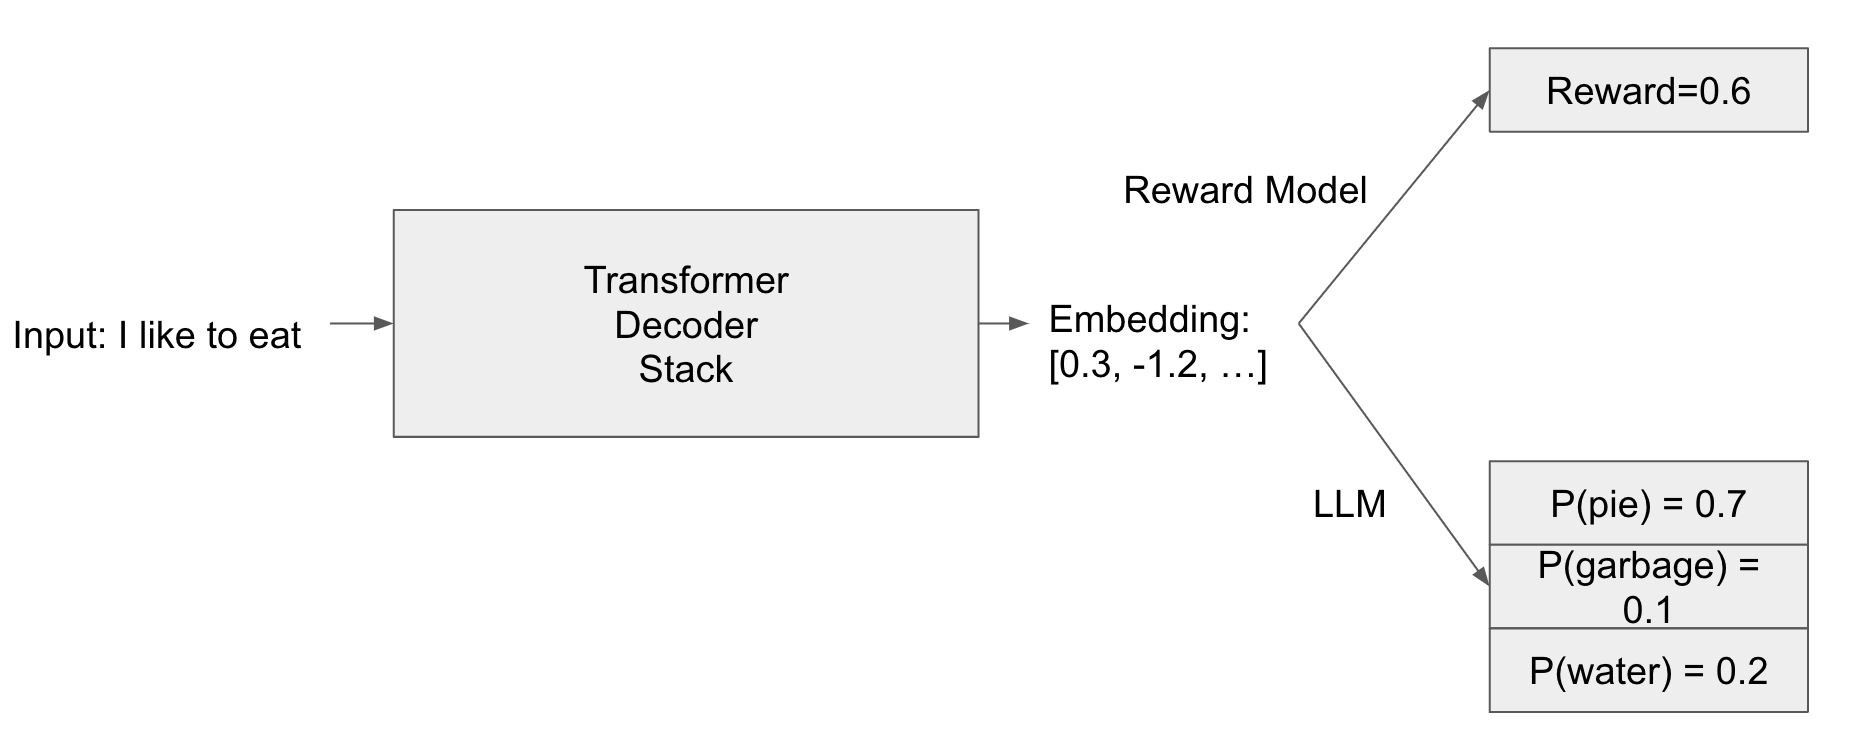
\includegraphics{src/Figures/arch.png}

}

\caption{\label{fig-rm-arch}Overall architecture of a reward model based
on LLM}

\end{figure}%

The Llama2 reward model (\citeproc{ref-2307.09288}{Touvron et al. 2023})
is initialized from the pretrained Llama2 LLM. In the LLM, the last
layer is a mapping \(L: \mathbb{R}^D \rightarrow \mathbb{R}^V\), where
\(D\) is the embedding dimension from the transformer decoder stack and
\(V\) is the vocabulary size. To get the RM, we replace that last layer
with a randomly initialized scalar head that maps
\(L: \mathbb{R}^D \rightarrow \mathbb{R}^1\). It's important to
initialize the RM from the LLM it's meant to evaluate. This is because:

\begin{enumerate}
\def\labelenumi{\arabic{enumi}.}
\item
  The RM will have the same ``knowledge'' as the LLM. This is
  particularly useful if evaluating things like ``does the LLM know when
  it doesn't know?''. However, in cases where the RM is simply
  evaluating helpfulness or factuality, it may be useful to have the RM
  know more.
\item
  The RM is on distribution for the LLM - it is initialized in a way
  where it semantically understands the LLM's outputs.
\end{enumerate}

An RM is trained with paired preferences, following the format:
\[\begin{aligned}
    \langle prompt\_history, response\_accepted, response\_rejected \rangle
\end{aligned}\] Prompt\_history is a multiturn history of user prompts
and model generations, response\_accepted is the preferred final model
generation by an annotator, and response\_rejected is the unpreferred
response. The RM is trained with a binary ranking loss with an optional
margin term m(r), shown in equation (7). There is also often a small
regularization term added to center the score distribution on 0.
\[\mathcal{L}_{\text{ranking}} = -\log(\sigma(r_\theta(x,y_c) - r_\theta(x,y_r) - m(r)))\]
The margin term increases the distance in scores specifically for
preference pairs annotators rate as easier to separate.

\begin{longtable}[]{@{}lcccc@{}}
\caption{Two variants of preference rating based margin with different
magnitude.}\label{tbl-margin_nums}\tabularnewline
\toprule\noalign{}
\endfirsthead
\endhead
\bottomrule\noalign{}
\endlastfoot
& Significantly & Better & Slightly & Negligibly \\
& Better & & Better & Better / Unsure \\
Margin Small & 1 & 2/3 & 1/3 & 0 \\
Margin Large & 3 & 2 & 1 & 0 \\
\end{longtable}

\begin{figure}

\centering{

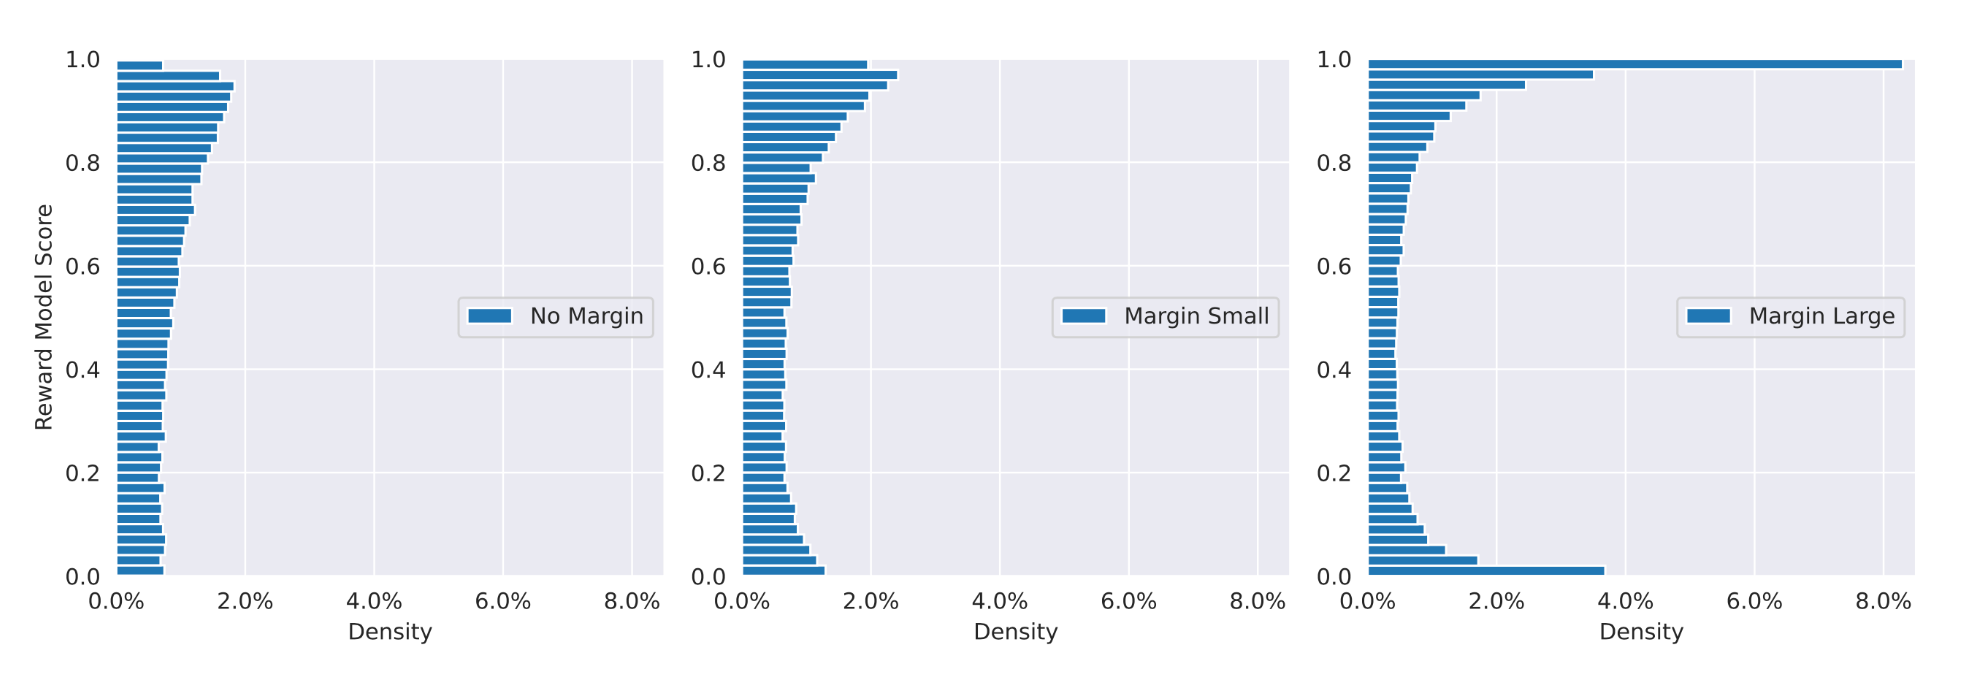
\includegraphics{src/Figures/margin-2.png}

}

\caption{\label{fig-margin-2}Reward model score distribution shift
caused by incorporating preference rating based margin in ranking loss.
With the margin term, we observe a binary split pattern in reward
distribution, especially for a larger margin.}

\end{figure}%

It may seem confusing how the margins were chosen. It's primarily
because the sigmoid function, which is used to normalize the raw reward
model score, flattens out beyond the range of \([-4, 4]\). Thus, the
maximum possible margin is eight.

When training or using a reward model, watching for the following is
important:

\begin{enumerate}
\def\labelenumi{\arabic{enumi}.}
\item
  \textbf{LLM Distribution Shift}: With each finetune of the LLM, the RM
  should be updated through a collection of fresh human preferences
  using generations from the new LLM. This ensures that the RM stays
  aligned with the current distribution of the LLM and avoids drifting
  off-distribution.
\item
  \textbf{RM and LLM are coupled}: An RM is generally optimized to
  distinguish human preferences more efficiently within the specific
  distribution of the LLM to be optimized. However, this specialization
  poses a challenge: such an RM will underperform when dealing with
  generations not aligned with this specific LLM distribution, such as
  generations from a completely different LLM.
\item
  \textbf{Training Sensitivities of RMs}: Training RMs can be unstable
  and prone to overfitting, especially with multiple training epochs.
  It's generally advisable to limit the number of epochs during RM
  training to avoid this issue.
\end{enumerate}

The industry has centered around optimizing for two primary qualities in
LLMs: helpfulness and harmlessness (safety). There are also other axes
such as factuality, reasoning, tool use, code, multilingual, and more,
but these are out of scope for us. In the Llama2 paper, preference data
was collected from humans for each quality, with separate guidelines.
This presents a challenge for co-optimizing the final LLM towards both
goals.

Two main approaches can be taken for Reinforcement Learning from Human
Feedback (RLHF) in this context:

\begin{enumerate}
\def\labelenumi{\arabic{enumi}.}
\item
  Train a unified reward model that integrates both datasets.
\item
  Train two separate reward models, one for each quality, and optimize
  the LLM toward both.
\end{enumerate}

Option 1 is difficult because of the tension between helpfulness and
harmlessness. They trade off against each other, confusing an RM trained
on both. The chosen solution was option 2, where two RMs are used to
train the LLM in a piecewise fashion. The helpfulness RM is used as the
primary optimization term, while the harmlessness RM acts as a penalty
term, driving the behavior of the LLM away from unsafe territory only
when the LLM veers beyond a certain threshold. This is formalized as
follows, where \(R_s\), \(R_h\), and \(R_c\) are the safety,
helpfulness, and combined reward, respectively. \(g\) and \(p\) are the
model generation and the user prompt: \[\begin{aligned}
    R_c(g \mid p) =
    \begin{cases}
        R_s(g \mid p) & \text{if } \text{is\_safety}(p) \text{ or } R_s(g \mid p) < 0.15 \\
        R_h(g \mid p) & \text{otherwise}
    \end{cases}
\end{aligned}\]

There are several open issues with reward models alluded to in the
paper. For example, how best to collect human feedback? Training
annotators and making sure they do the correct thing is hard. What
should the guidelines be? Another question is whether RMs can be made
robust to adversarial prompts. Last but not least, do RMs have
well-calibrated scores? This matters for RLHF - pure preference accuracy
isn't enough.

\subsection{Reward Learning in
Robotics}\label{reward-learning-in-robotics}

To help set up our basic reward learning problem, consider a user and a
robot. The user's preferences or goals can be represented by an internal
reward function, R(\(\xi\)), which the robot needs to learn. Since the
reward function isn't explicit, there are a variety of ways that the
robot can learn this reward function, which we will discuss in the next
section. An example method of learning a reward function from human data
is using pairwise comparison. Consider the robot example from section
one, but now, the robot shows the human two possible trajectories
\(\xi_A\) and \(\xi_B\) as depicted in the diagram below.

\begin{figure}

\centering{

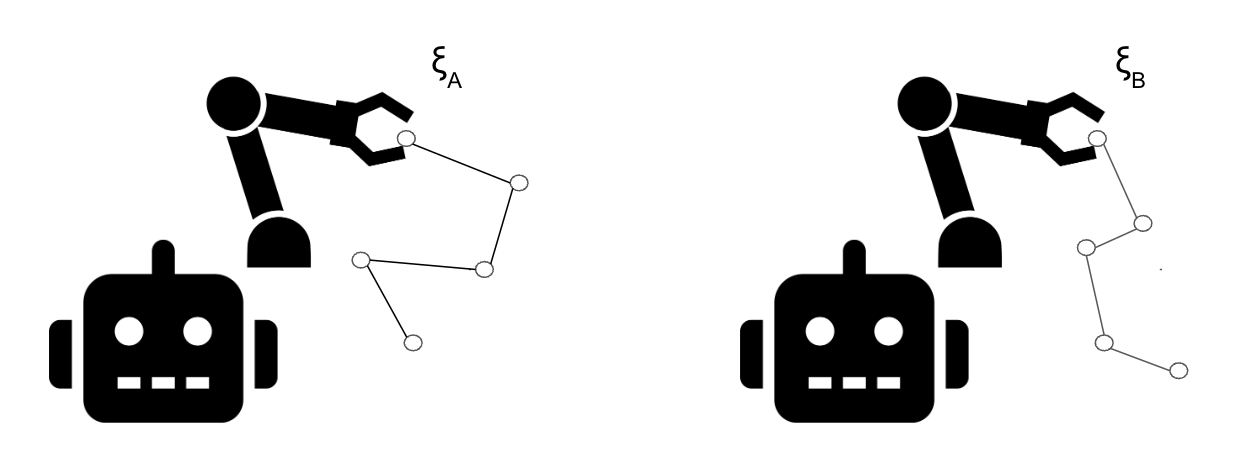
\includegraphics[width=0.7\textwidth,height=\textheight]{src/Figures/robots.png}

}

\caption{\label{fig-reward-robot-1}Two different trajectories taken by a
robot to prompt user ranking.}

\end{figure}%

The user is show both the trajectories above and asked to rank which one
is better. Based on iterations of multiple trajectories and ranking, the
robot is able to learn the user's internal reward function. There quite
a lot of ways that models can learn a reward function from human data.
Here's a list (\citeproc{ref-myers2021learning}{Myers et al. 2021}) of
some of them:

\begin{enumerate}
\def\labelenumi{\arabic{enumi}.}
\item
  Pairwise comparison: This is the method that we saw illustrated in the
  previous example. The robot is able to learn based on a comparison
  ranking provided by the user.
\item
  Expert demonstrations: Experts perform the task and the robot learns
  the optimal reward function from these demonstrations.
\item
  Sub-optimal demonstrations: The robot is provided with demonstrations
  that are not quite as good as the expert demonstrations but it is
  still able to learn a noisy reward function from the demonstrations.
\item
  Physical Corrections: While the robot is performing the task, at each
  point in its trajectory (or at an arbitrary point in its trajectory)
  its arm is corrected to a more suitable position. Based on these
  corrections, the robot is able to learn the reward function.
\item
  Ranking: This method is similar to pairwise comparison but involves
  more trajectories than 2. All the trajectories may have subtle
  differences from each other, but these differences help provide
  insight to the model.
\item
  Trajectory Assessment: Given a single trajectory, the user rates how
  close it is to optimal, typically using a ranking scale.

  Each of these methods allows the robot to refine its understanding of
  the user's reward function, but their effectiveness can vary depending
  on the application. For instance, expert demonstrations tend to
  produce more reliable results but may not always be feasible in
  everyday tasks. Pairwise comparison and ranking methods offer more
  flexibility but might require a higher number of iterations.
\end{enumerate}

\subsection{Reward Learning with Meta
Learning}\label{reward-learning-with-meta-learning}

Learning a reward function from human preferences is an intricate and
complicated task. At its core, this task is about designing algorithms
that can capture what humans value based on their elicited preferences.
However, due to the nuanced and multifaceted nature of human desires,
learning reward functions from human can be a difficult task. Therefore,
meta-learning rewards may be considered to facilitate the reward
learning processes. Meta-learning, often referred to as ``learning to
learn,'' aims to design models that can adapt to new tasks with minimal
additional efforts. We discuss paper (\citeproc{ref-hejna2023few}{Hejna
III and Sadigh 2023}) in Section~\ref{sec-few-shot} showing how
meta-learning can be leveraged for few-shot preference learning, where a
system can quickly adapt to a new task after only a few queries to
pairwise preferences from human.

Moving beyond the concept of learning from pairwise preferences, in
Section~\ref{sec-watch} we discuss a different approach where
meta-learning intersects with both demonstrations and rewards
(\citeproc{ref-zhou2019watch}{Zhou et al. 2019}). This paper considers
the use of both demonstrations and rewards elicited from human that
guide the learning process.

In the regular learning setting, a model is fitted to a dataset with
certain learning algorithm. The learning algorithm, for example, can be
the minimization of a loss function. To formulate the ``regular''
learning procedure, let's denote the training dataset as \(D\), and the
test dataset as \(S\). Given a model parameterized by \(\theta\);
training loss function \(L(\theta, D)\); and test loss function
\(L(\theta, S)\), we can formulate a process of ``regular'' machine
learning process as \[\begin{aligned}
    \theta^\star = \arg\min_\theta\quad L(\theta, D).
\end{aligned}\] Note that the minimization of the training loss function
is essentially \emph{one} possible learning algorithm. For example,
instead of minimizing the loss function, one may do gradient descent
with model regularization on the loss function, where the final solution
may not be the one that actually minimizes the loss function. As a
result, we may want to be more general and more abstract for the moment,
and denote the learning algorithm as \(\mathcal{A}\). Thus, we can write
\[\begin{aligned}
    \theta^\star = \mathcal{A}(D),
\end{aligned}\] i.e., the learning algorithm \(\mathcal{A}\) takes in a
training dataset and outputs a model parameter \(\theta^\star\). Then,
the performance of the model is evaluated by the test loss
\(L(\mathcal{A}(D), S)\). As we can see, in the regime of ``regular''
learning, the learning algorithm \(\mathcal{A}\) is pre-defined and
fixed.

Meta-learning, or learning-to-learn, essentially asks the question of
whether one can \emph{learn} the learning algorithm \(\mathcal{A}\) from
prior tasks, such that the modal can adapt to a new task more
quickly/proficiently. For example, different human languages share
similar ideas, and therefore a human expert who has learned many
languages should be able to learn a new language easier than an average
person. In other words, the human expert should have learned how to
learn new languages more quickly based on their past experiences on
learning languages.

To mathematically formulate meta-learning, we consider a family of
learning algorithms \(\mathcal{A}_\omega\) parameterized by \(\omega\).
The ``prior'' tasks are represented by a set of meta-training datasets
\(\{(D_i, S_i)\}_{i=1}^N\) consists of \(N\) pairs of training dataset
\(D_i\) and test dataset \(S_i\). As we noted before, a learning
algorithm \(\mathcal{A}_\omega\) takes in a training dataset, and
outputs a model, i.e., \[\begin{aligned}
    \forall i: \quad \theta^\star_i=\mathcal{A}_\omega(D_i).
\end{aligned}\]

Therefore, the \textbf{meta-learning objective} is \[\begin{aligned}
    \min_\omega \quad \sum_{i}\ L(\mathcal{A}_\omega(D_i), S_i).
\end{aligned}\] The above optimization problem gives a solution
\(\omega^\star\) which we use as the meta-parameter. Then, when a new
task comes with a new training dataset \(D_{new}\), we can simply apply
\(\theta^\star_{new}=\mathcal{A}_{\omega^\star}(D_{new})\) to obtain the
adapted model \(\theta^\star_{new}\). Note that we usually assume the
meta-training datasets \(D_i, S_i\) and the new dataset \(D_{new}\)
share the same underlying structure, or they come from the same
distribution of datasets.

One of the most popular meta-learning method is Model-Agnosic
Meta-Learning (MAML) (\citeproc{ref-finn2017model}{Finn, Abbeel, and
Levine 2017}). In MAML, the meta-parameter \(\omega\) shares the same
space as the model parameter \(\theta\). At its core, in MAML the
learning algorithm is defined to be \[\begin{aligned}
    \mathcal{A}_\omega(D_i)=\omega-\alpha \nabla_\omega L(\omega, D_i),
\end{aligned}\] where \(\alpha\) is the step size. As we can see, in
fact \(\omega\) is defined as the initialization of fine-tuning
\(\theta\). With a good \(\omega\) learned, the model can adapt to a new
task very quickly. In general, meta-learning can be summarized as
follows: Given data from prior tasks, learn to solve a new task more
quickly/proficiently. Given the general nature of meta-learning, one may
be curious about whether preference learning can be benefited from
meta-learning, which we discuss in the following section.

\subsubsection{Few-Shot Preference Learning for Reinforcement
Learning}\label{sec-few-shot}

Reinforcement learning (RL) in robotics often stumbles when it comes to
devising reward functions aligning with human intentions.
Preference-based RL algorithms aim to solve this by learning from human
feedback, but this often demands a \emph{highly impractical number of
queries} or leads to oversimplified reward functions that don't hold up
in real-world tasks.

To address the impractical requirement of human queries, as we discussed
in the previous section, one may apply meta-learning so that the RL
agent can adapt to new tasks with fewer human queries.
(\citeproc{ref-hejna2023few}{Hejna III and Sadigh 2023}) proposes to
pre-training models on previous tasks with the meta-learning method MAML
(\citeproc{ref-finn2017model}{Finn, Abbeel, and Levine 2017}), and then
the meta-trained model can adapt to new tasks with fewer queries.

We consider Reinforcement Learning (RL) settings where a state is
denoted as \(s\in S\), and action is denoted as \(a\in A\), for state
space \(S\) and action space \(A\). The reward function
\(r:S\times A \to \mathbb{R}\) is unknown and need to be learned from
eliciting human preferences. There are multiple tasks, where each task
has its own reward function and transition probabilities. The reward
model is parameterized by \(\psi\). We denote \(\hat{r}_\psi(s,a)\) to
be a learned estimate of an unknown ground-truth reward function
\(r(s,a)\), parameterized by \(\psi\). Accordingly, a reward model
determines a RL policy \(\phi\) by maximizing the accumulated rewards.
The preferences is learned via pairwise comparison of trajectory
segments \[\begin{aligned}
    \sigma = (s_t, a_t, s_{t+1}, a_{t+1}, ..., s_{t+k-1}, s_{t+k-1})
\end{aligned}\] of \(k\) states and actions.

For each pre-training task, there is a dataset \(D\) consists of labeled
queries \((\sigma_1, \sigma_2, y)\) where \(y\in \{0, 1\}\) is the label
representing which trajectory is preferred. Therefore, a loss function
\(L(\psi, D)\) captures how well the reward model characterizes the
preferences in dataset \(D\). In (\citeproc{ref-hejna2023few}{Hejna III
and Sadigh 2023}) they the preference predictor over segments using the
Bradley-Terry model of paired comparisons
(\citeproc{ref-bradley1952rank}{Bradley and Terry 1952a}), i.e.,
\[\begin{aligned}
    P[\sigma_1 \succ \sigma_2 ] = \frac{\exp \sum_t \hat{r}_\psi(s_t^{1}, a_t^{1})}{\exp \sum_t \hat{r}_\psi(s_t^{1}, a_t^{1}) + \exp \sum_t \hat{r}_\psi(s_t^{2}, a_t^{2})}.
\end{aligned}\] Then, the loss function is essentially a binary
cross-entropy which the reward model \(\psi\) aims to minimize, i.e.,
\[\begin{aligned}
    {L}(\psi,  {D}) = - \mathbb{E}_{(\sigma^1, \sigma^2, y) \sim {D}} \left[ y(1) \log (P[\sigma_1 \succ \sigma_2 ]) + y(2)\log(1 - P[\sigma_1 \succ \sigma_2 ]) \right].
\end{aligned}\]

\paragraph*{Method Component 1: Pre-Training with Meta
Learning}\label{method-component-1-pre-training-with-meta-learning}
\addcontentsline{toc}{paragraph}{Method Component 1: Pre-Training with
Meta Learning}

To efficiently approximate the reward function \(r_\text{new}\) for a
new task with minimal queries, as described in
(\citeproc{ref-hejna2023few}{Hejna III and Sadigh 2023}), we aim to
utilize a pre-trained reward function \(\hat{r}_\psi\) that can be
quickly fine-tuned using just a few preference comparisons. By
pre-training on data from prior tasks, we can leverage the common
structure across tasks to speed up the adaptation process. Although any
meta-learning method is compatible, (\citeproc{ref-hejna2023few}{Hejna
III and Sadigh 2023}) opt for Model Agnostic Meta-Learning (MAML) due to
its simplicity. Therefore, the pre-training update for the reward model
\(\psi\) is \[\begin{aligned}
    \psi \xleftarrow{} \psi - \beta \nabla_\psi \sum_{i = 1}^N {L} (\psi - \alpha \nabla_\psi {L}(\psi, {D}_i), {D}_i),
\end{aligned}\] where \(\alpha, \beta\) are the inner and outer learning
rate, respectively. We note that data \(\{D_i\}_i\) of labeled
preferences queries for prior tasks can come from offline datasets,
simulated policies, or actual humans.

\paragraph*{Method Component 2: Few-Shot
Adaptation}\label{method-component-2-few-shot-adaptation}
\addcontentsline{toc}{paragraph}{Method Component 2: Few-Shot
Adaptation}

With the aforementioned pre-training with meta learning, the
meta-learned reward model can then be used for few-shot preference based
RL during an online adaptation phase. The core procedure of the few-shot
adaption is descibed as below

\begin{enumerate}
\def\labelenumi{\arabic{enumi}.}
\item
  Given a pre-trained reward model \(\psi\)
\item
  For time step \(t=1, 2, \dots\)

  \begin{enumerate}
  \def\labelenumii{\arabic{enumii}.}
  \item
    Find pairs of trajectories \((\sigma_1, \sigma_2)\) with preference
    uncertainty based on \(\psi\).
  \item
    Query human preference \(y\) and forms a new dataset \(D_{new}\)
  \item
    Update the reward model by
    \(\psi'\leftarrow \psi - \alpha \nabla_\psi L(\psi, D_{new})\)
  \item
    Update the policy with the new reward model \(\psi'\)
  \end{enumerate}
\end{enumerate}

As mentioned in (\citeproc{ref-hejna2023few}{Hejna III and Sadigh
2023}), uncertain queries are selected using the disagreement of an
ensemble of reward functions over the preference predictors.
Specifically, comparisons that maximize
\(\texttt{std}(P[\sigma_1 \succ \sigma_2])\) are selected each time
feedback is collected.

The whole pipeline of the method is outlined in Figure~\ref{fig-few-1}.

\begin{figure}

\centering{

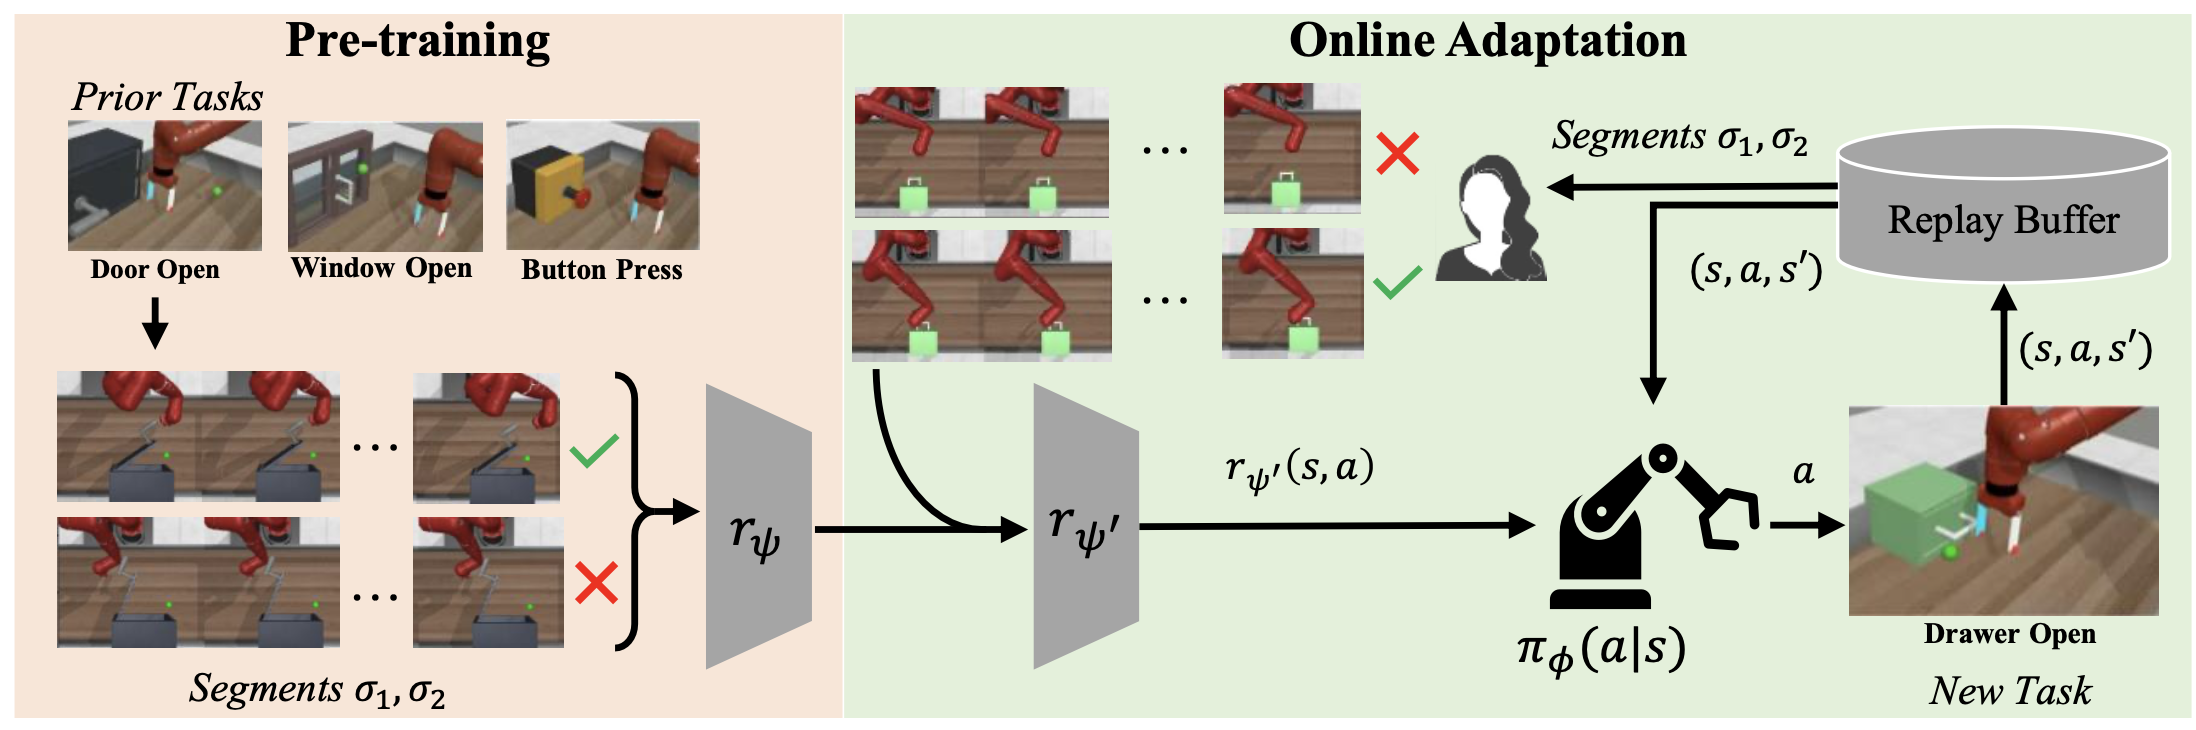
\includegraphics{src/Figures/overview-few.png}

}

\caption{\label{fig-few-1}An overview of the proposed method in
(\citeproc{ref-hejna2023few}{Hejna III and Sadigh 2023}).
\textbf{Pre-training (left):} In the pre-training phase, trajectory
segment comparisons are generated using data from previously learned
tasks. Then, they are used to train a reward model.
\textbf{Online-Adaptation (Right)}: After pre-training the reward model,
it is adapted to new data from human feedback. The adapted reward model
is then used to train a policy for a new task in a closed loop manner.}

\end{figure}%

We present one set of experiment from the paper, as it illustrates the
effectiveness of the proposed method in a straightforward way. The
experiment test the propoesed method on the Meta-World benchmark
(\citeproc{ref-yu2020meta}{Yu et al. 2020}). Three baselines are
compared with the proposed method:

\begin{enumerate}
\def\labelenumi{\arabic{enumi}.}
\item
  SAC: The Soft-Actor Critic RL algorithm trained from ground truth
  rewards. This represents the standard best possible method given the
  ground-truth reward.
\item
  PEBBLE: The PEBBLE algorithm (\citeproc{ref-lee2021pebble}{Lee, Smith,
  and Abbeel 2021}). It does not use information from pripor tasks.
\item
  Init: This method initialize the reward model with the pretained
  weights from meta learning. However, instead of adapting the reward
  model to the new task, it performs standard updates as in PEBBLE.
\end{enumerate}

The results are shown in Figure~\ref{fig-few-exp}, where we can see that
the proposed methord outperforms all of the baselines.

\begin{figure}

\centering{

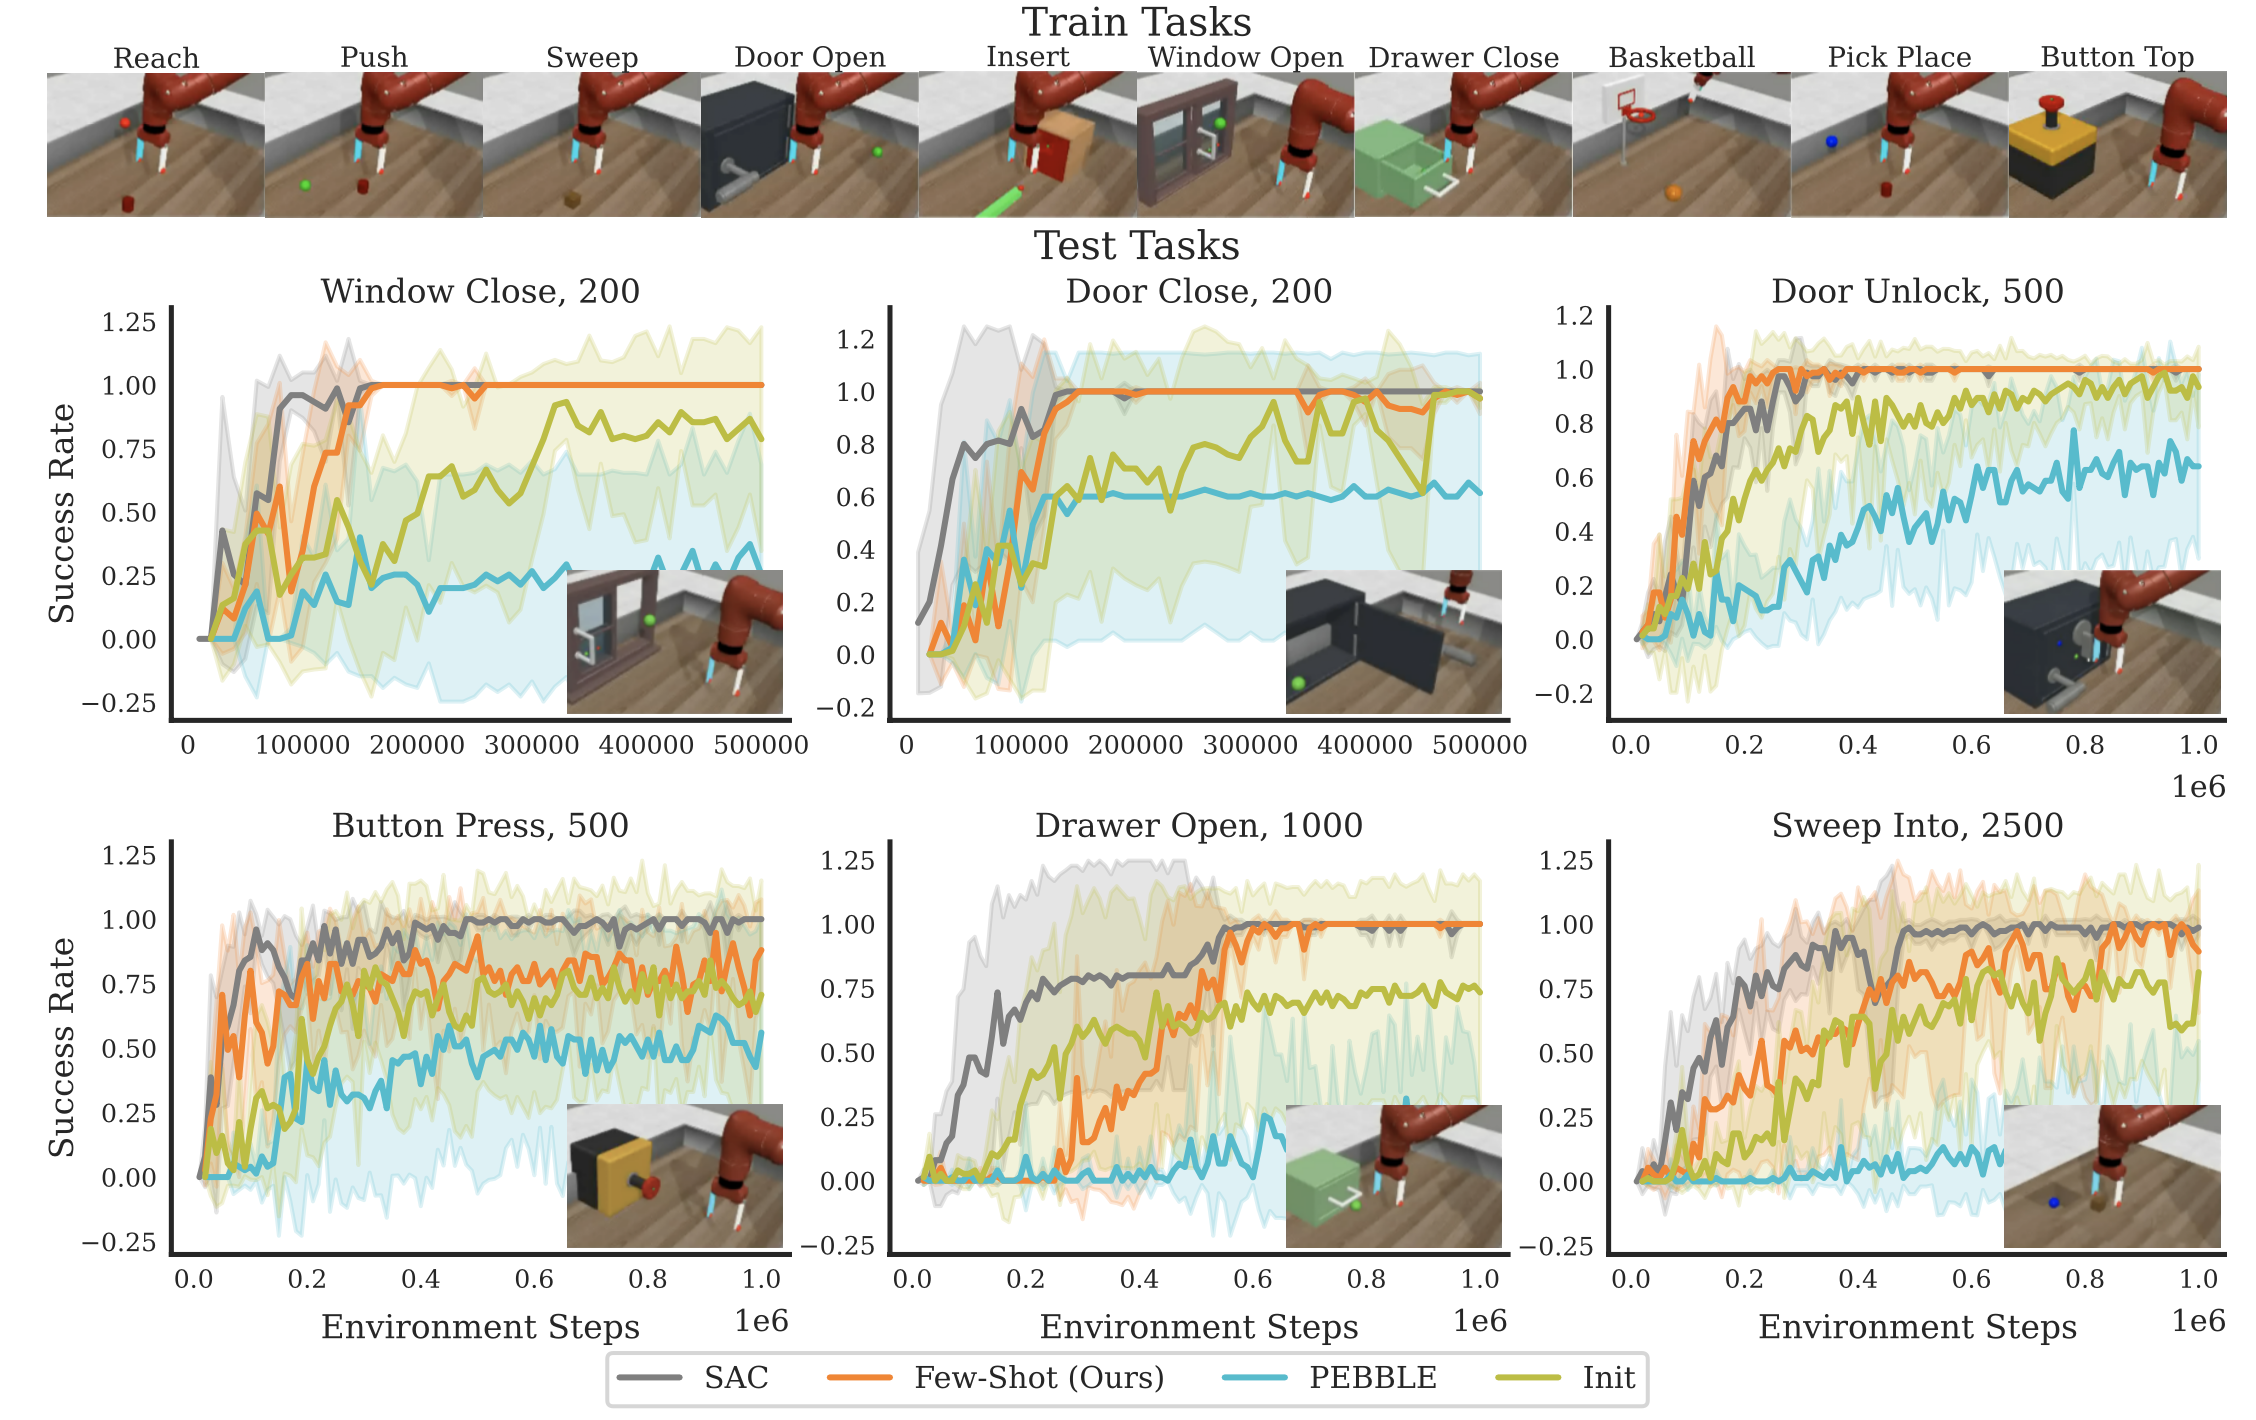
\includegraphics{src/Figures/few-exp.png}

}

\caption{\label{fig-few-exp}Results on MetaWorld tasks. The title of
each subplot indicates the task and number of artificial feedback
queries used in training. Results for each method are shown across five
seeds.}

\end{figure}%

This paper (\citeproc{ref-hejna2023few}{Hejna III and Sadigh 2023})
shows that meta reward learning indeed reduce the number of queries of
human preferences. However, as mentioned in the paper, there are still
some drawbacks, as shown in the following.

Many of the queries the model pick for human preference elicitation are
actually almost identical to human. After all, the model would pick the
most uncertain pair of trajectories for human preference queries, and
similar trajectories are for sure having high uncertainty in their
preference. This suggest the need of new ways for designing the query
selection strategy.

Moreover, despite the improved query complexity, it still needs an
impractical amount of queries. As shown in Figure~\ref{fig-few-exp}, the
``sweep into'' task still needs 2500 human queries for it to work
properly, which is still not ideal for what we want them to be.

In addition, it is mentioned in the paper that the proposed method may
be even worse than training from scratch, if the new task is too
out-of-distribution. Certainly, since meta-learning assumes
in-distribution tasks, we cannot expect the proposed method to be good
for out-of-distribution task. It is thus an interesting future direction
to investigate whether one can design a method that automatically
balance between using the prior information or training from scratch.

\subsubsection{Watch Try Learn}\label{sec-watch}

Watch, Try, Learn: Meta-Learning from Demonstrations and Rewards
(\citeproc{ref-zhou2019watch}{Zhou et al. 2019}) asks the question ``How
can we efficiently learn both from expert demonstrations and from trials
where we only get \textbf{binary} feedback from a human". Why do we care
about this question? In the context of robotics, a very compelling
answer is the \emph{cost of data-collection}. In a hypothetical world in
which we have a vast number of \textbf{expert demonstrations} of robots
accomplishing a large number of diverse tasks, we don't necessarily need
to worry about learning from trials or from humans. We could simply
learn a very capable imitation agent to perform any task. Natural
Language Processing could be seen as living in this world, because
internet-scale data is available. \textbf{Robots, however, are
expensive}, so people generally don't have access to them, and therefore
cannot use them to produce information to imitate. Similarly,
\textbf{human time is expensive}, so even for large organizations that
do have access to a lot of robots, it's still hard to collect a lot of
expert demonstrations.

The largest available collection of robotics datasets today is Open
X-Embodiment ((\citeproc{ref-padalkar2023open}{Padalkar et al. 2023})),
which consists of around 1M episodes from more than 300 different
scenes. Even such large datastes are not enough to learn
generally-capable robotic policies from imitation learning alone.

\begin{figure}

\centering{

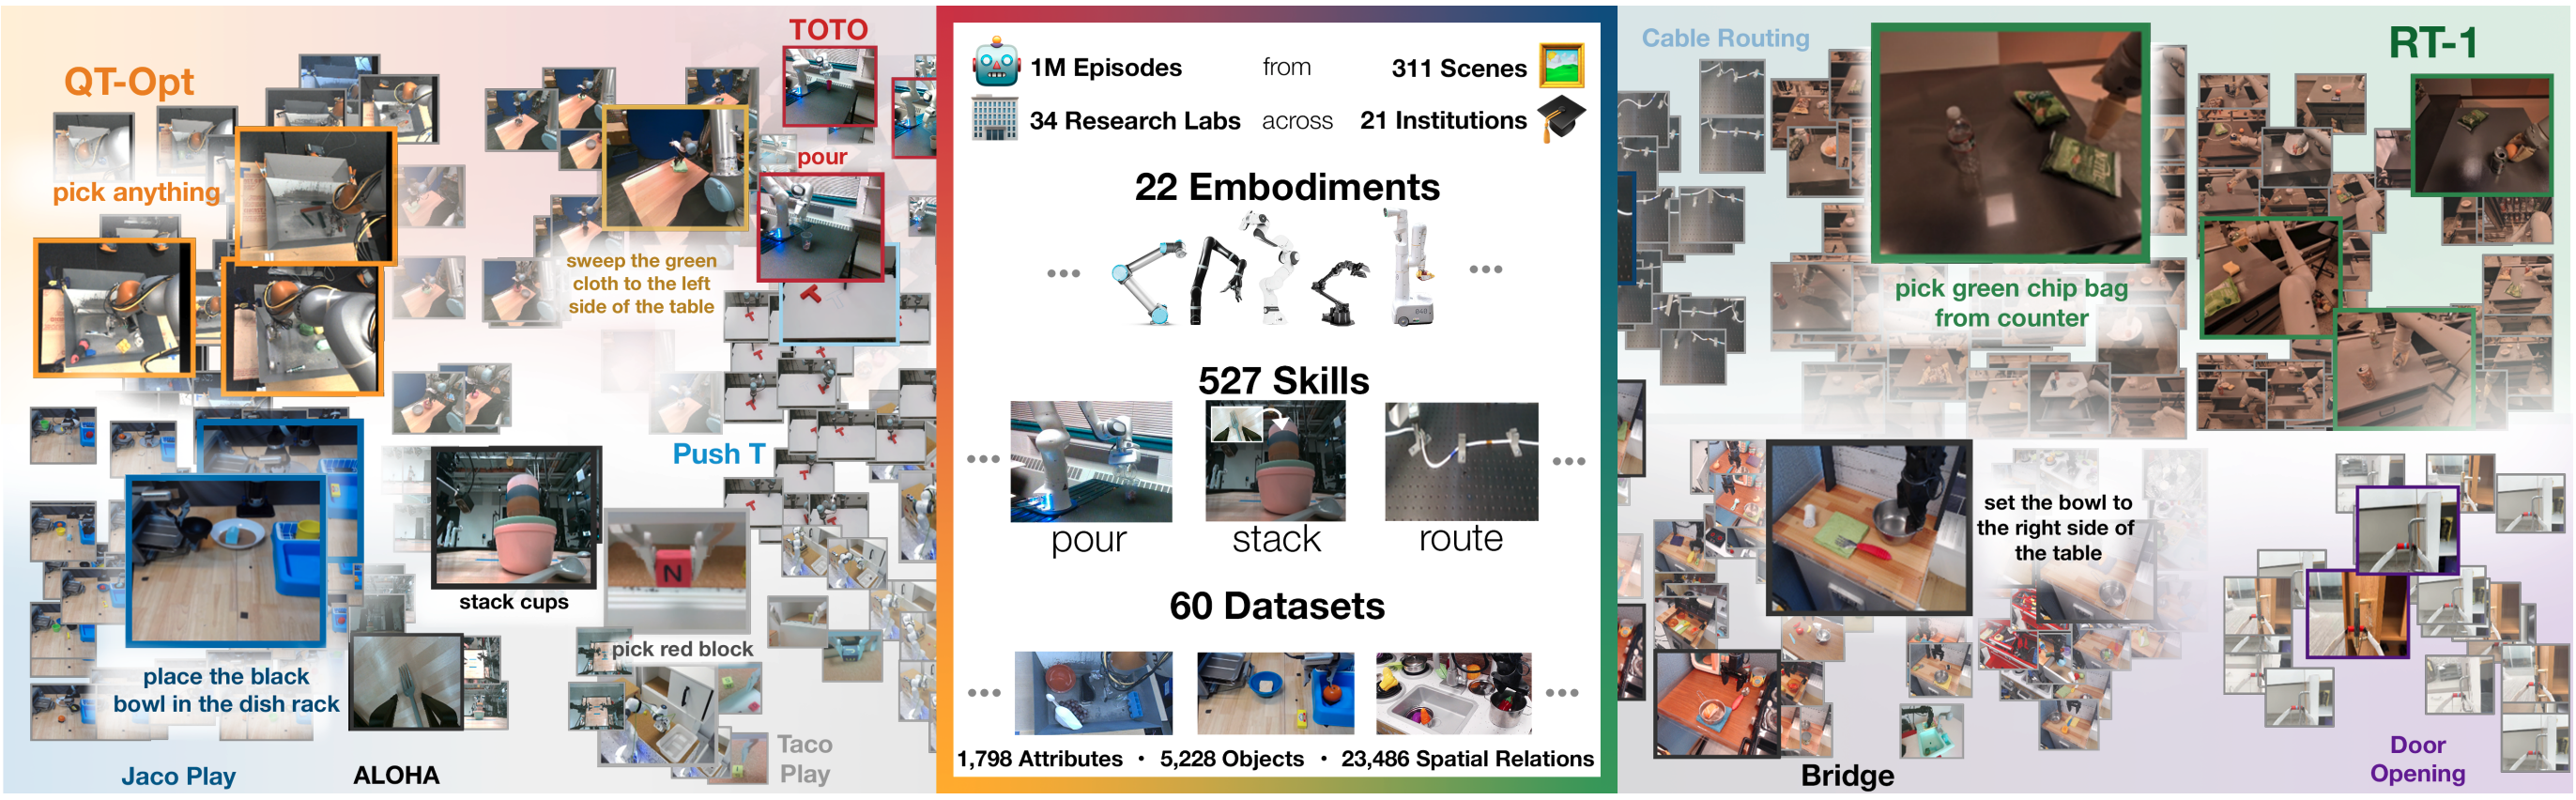
\includegraphics{src/Figures/open_x_embodiment.png}

}

\caption{\label{fig-open-x-embodiment}Visualization of the Open
X-Embodiment dataset collection. Even this large-scale dataset for robot
learning is not yet enough to learn generally-capable robotic policies.}

\end{figure}%

\textbf{Main insight:} binary feedback is much cheaper to obtain than
expert demonstrations! Instead of hiring people to act as robot
operators to tell the robot exactly what to do, if there was a way of
having many robots trying things in parallel, we can have humans watch
videos of what the robots did and then give a success classification of
whether the robot accomplished the goal. This is a much cheaper form of
human supervision because the human labels don't necessarily need to be
given in real time, so one human labeler can label many trajectories in
parallel, and the human doesn't need to be a skilled robot operator.

Concretely, this paper seeks to learn new tasks with the following
general problem setting:

\begin{enumerate}
\def\labelenumi{\arabic{enumi}.}
\item
  We only get 1 expert demonstration of the target task
\item
  After seeing the expert demonstration, we have robots try to solve the
  task 1 or more times.
\item
  The user (or some pre-defined reward function) annotates each trial as
  success/failure.
\item
  The agent learns from both the demos and the annotated trials to
  perform well on the target task.
\end{enumerate}

Note that this work falls under the \textbf{meta-learning} umbrella,
because we are learning an algorithm for quickly learning new tasks
given new observations (demos, trials, and success labels.)

The \textbf{main contribution} of this paper is a meta-learning
algorithm for incorporating demonstrations and binary feedback from
trials to solve new tasks.

Meta-Learning deals with efficient learning of new tasks. In the context
of robotics or reinforcement learning in general, \textbf{how do we
define tasks}? We will use the Markov decision process (\textbf{MDP})
formalism. A task \(T_i\) is described with the tuple
\(\{S, A, r_i, P_i\}\).

\begin{enumerate}
\def\labelenumi{\arabic{enumi}.}
\item
  \(S\) represents the \emph{state-space} of the task, or all possible
  states the agent could find itself in. This work uses
  image-observations, so \(S\) is the space of all possible RGB images.
\item
  \(A\) is the action space, meaning the set of all possible actions the
  agent could take. In robotics there are many ways of representing
  action spaces, and this work considers end-effector positions,
  rotations, and opening.
\item
  \(r_i\) is the reward function for the task, with function signature
  \(r_i : S \times A \to \mathbb{R}\). This work assumes all reward
  functions are binary.
\item
  \(P_i\) is the transition dynamics function. It's a function that maps
  state-action pairs to probability distributions over next states.
\end{enumerate}

Notice that \(S\) and \(A\) are shared across tasks. Transition dynamics
functions are normally also shared between tasks because they represent
the laws of physics. However, this work considers environments with
different objects, so they don't share the dynamics function. Given this
definition for tasks, they assume that the tasks from the data that they
get come from some unknown task-generating distribution \(p(T)\).

Let's give a more precise definition of the problem statement considered
by \textbf{Watch, Try, Learn}. As the paper name suggests, there are 3
phases for the problem statement.

\textbf{Watch:} During the \emph{watch} phase, we give the agent \(K\)
demonstrations of the target tasks. This paper considers the case where
\(K\) always equals 1, and all demonstrations are successful. That is,
each demonstration consists of a trajectory
\(\{(s_0, a_0), \ldots, (s_H, a_H)\}\) where \(H\) is the task horizon,
and the final state is always successful, that is
\(r_i(s_H, a_H) = 1, r_i(s_j, a_j) = 0\) for every \(j \neq H\).

Importantly, these demonstrations alone might not be sufficient for
\textbf{full task specification}. As an example, consider a
demonstration in which an apple is moved to the right, next to a pan.
Seeing this demonstration alone, the task could be always moving the
apple to the right, or it could be always moving the apple next to the
pan, irrespective of where the pan is. The expected output after the
Watch phase is a policy capable of gathering information about a task,
given demonstrations.

\textbf{Try:} In the Try phase, we use the agent learned during the
Watch phase to attempt the task for \(L\) trials. As specified earlier,
this paper considers the casae where \(L\) always equals 1. After the
agent completes the trials, humans (or pre-programmed reward functions)
provide one binary reward for each trial, indicating whether the trial
was successful. The expected output of this phase is \(L\) trajectories
and corresponding feedback that hopefully \emph{disambiguate} the task.

\textbf{Learn:} After completing the trials, the agent must learn from
both the original expert demonstrations and the trials, and become
capable of solving the target task.

\textbf{Given Data:} To train agents that can Watch, Try, and Learn, we
are given a dataset of expert demonstrations containing multiple demos
for each task, and the dataset contains hundreds of tasks. Importantly,
\textbf{no online interaction} is needed for training, and this method
trains only with \textbf{supervised learning} and no reinforcement
learning.

This section describes exactly how this paper trains an agent from the
given expert demonstrations, and how to incorporate the trials and human
feedback into the loop.

\textbf{Training to Watch:} We now describe the algorithm to obtain an
agent conditioned on the given expert demonstration. In particular, what
we want to obtain out of the Watch phase is a policy conditioned on a
set of expert demonstrations. Formally, we want to obtain
\(\pi_\theta^{\text{watch}}(a | s, \{d_{i,k}\})\).

The way we can obtain this policy is through \textbf{meta-imitation
learning}. Given the demonstrations \(\{\textbf{d}_{i,k}\}\) for task
\(i\), we sample another \emph{different} demonstration coming from the
same task \(\textbf{d}_i^{\text{test}}\). The key insight here is that
\(\textbf{d}_i^{\text{test}}\) is an example of \textbf{optimal
behavior} given the demonstrations. Therefore, to obtain
\(\pi_\theta^{\text{watch}}(a | s, \{d_{i,k}\})\), we simply regress the
policy to imitate actions taken on \(\textbf{d}_i^{\text{test}}\).
Concretely, we train policy parameters \(\theta\) to minimize the
following loss:

\(\mathcal{L}^\text{watch}(\theta, \mathcal{D}_i^*) = \mathbb{E}_{\{d_{i,k}\} \sim \mathcal{D}_i^*} \mathbb{E}_{\{d_{i,k}^{\text{test}}\} \sim \mathcal{D}_i^*  \{d_{i,k}\}} \mathbb{E}_{(s_t, a_t) \sim d_i^{\text{test}}} \big[
- \log \pi_\theta^{\text{watch}} (a_t | s_t, \{d_{i,k}\}) \big]\)

This corresponds to doing imitation learning by minimizing the negative
log-likelihood of the test trajectory actions, conditioning the policy
on the entire demo set. However, how is the conditioning on the demo set
achieved?

\begin{figure}

\centering{

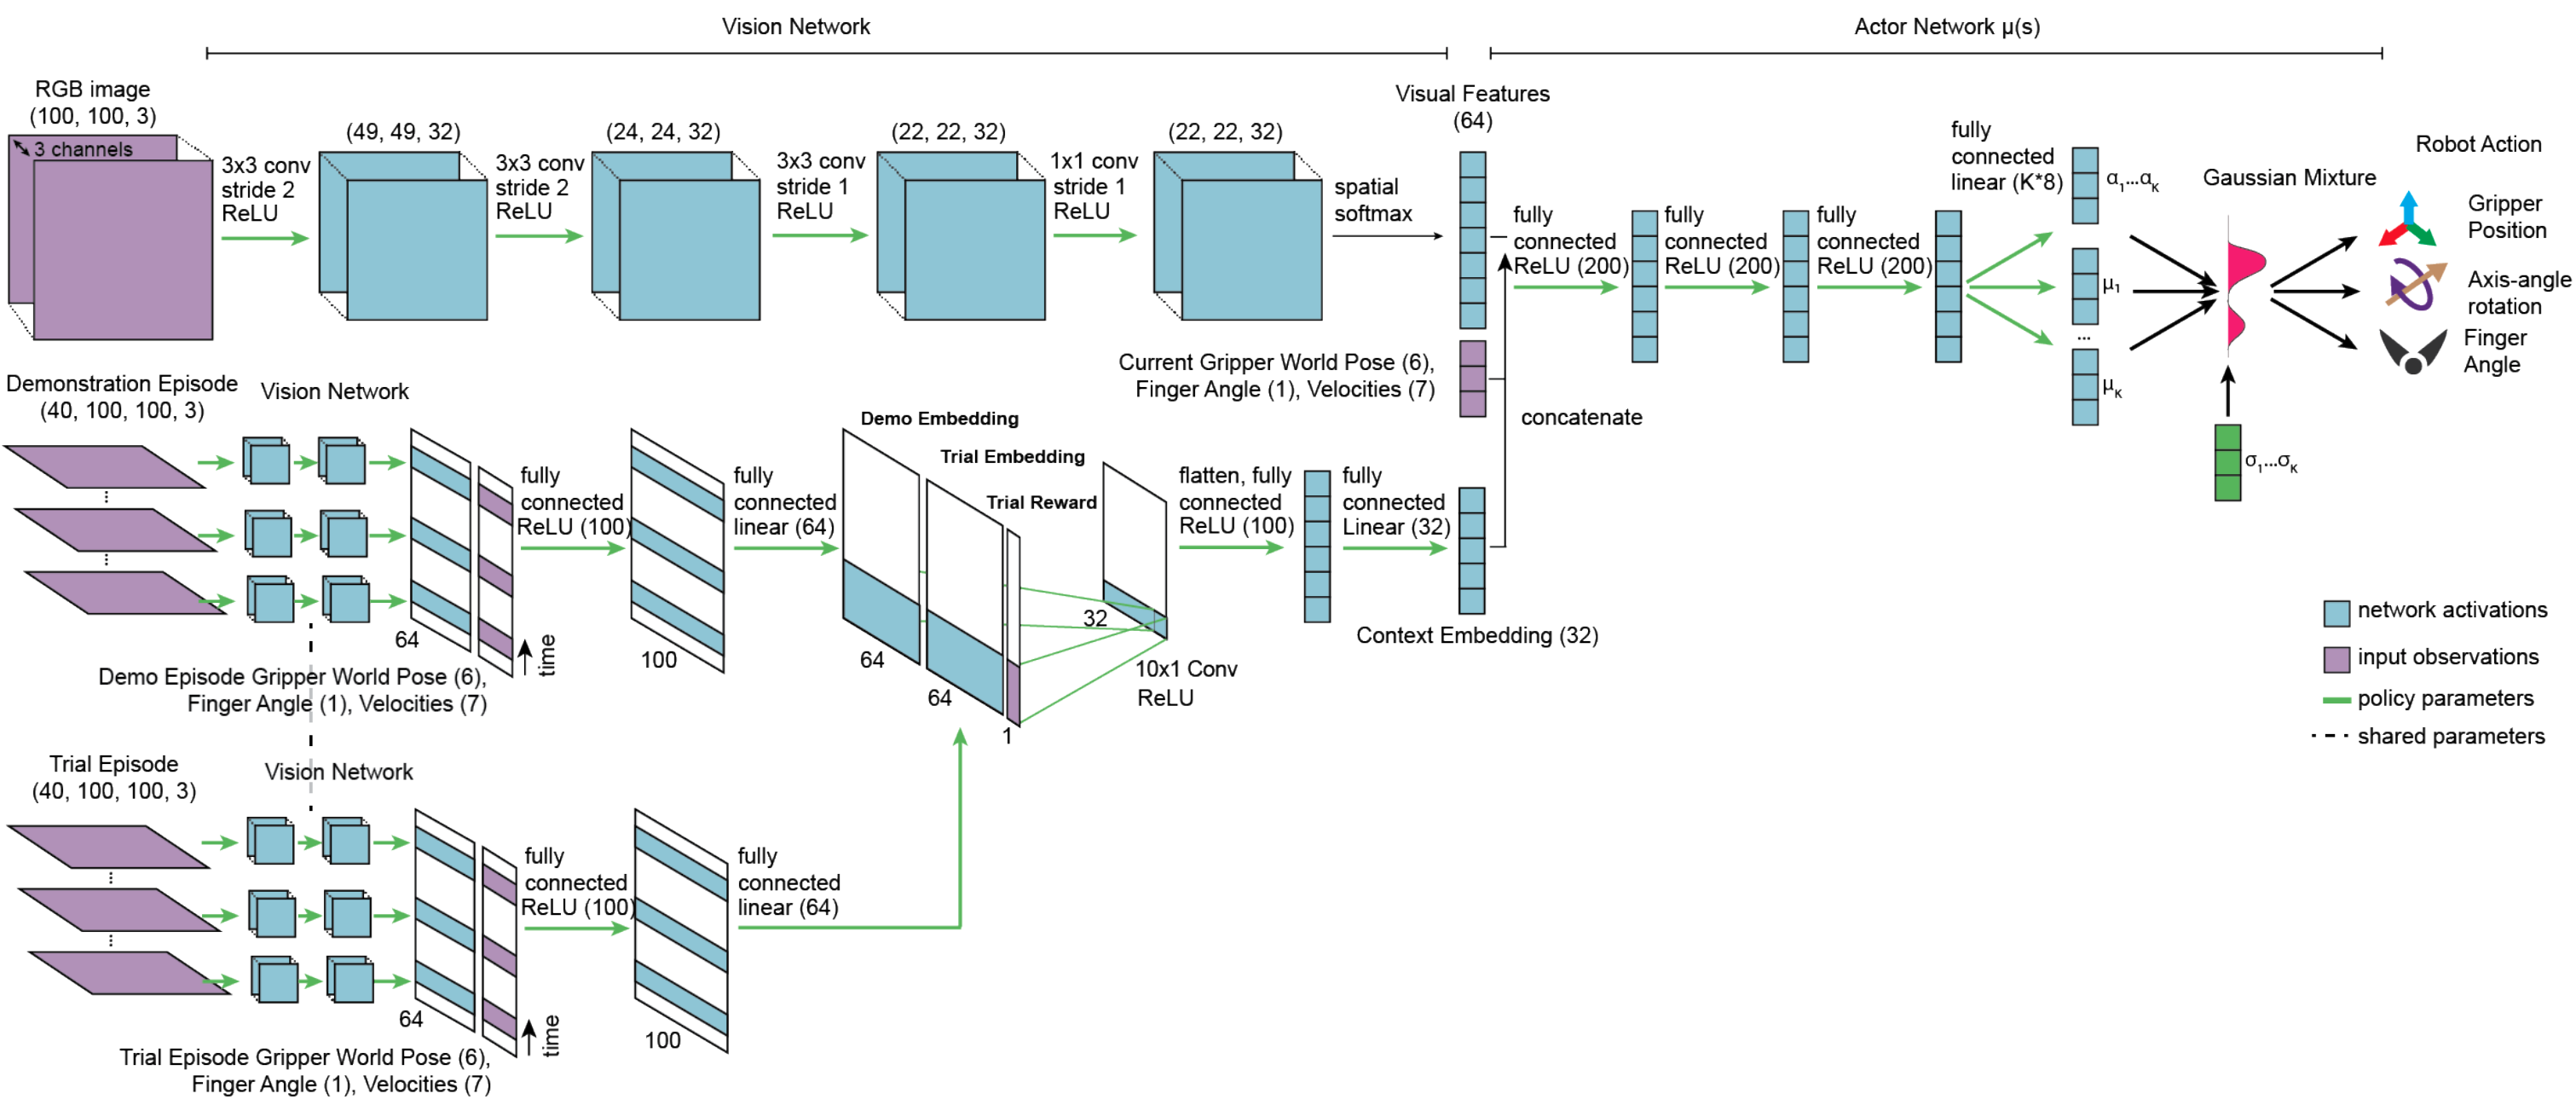
\includegraphics{src/Figures/watch-try-learn-architecture.png}

}

\caption{\label{fig-watch-try-learn-arch}Vision-based policy
architecture that conditions on a set of demonstrations.}

\end{figure}%

Figure~\ref{fig-watch-try-learn-arch} visualizes how Watch Try Learn
deals with conditioning on demonstrations. In addition to using features
obtained from the images of the current state, the architecture uses
features from frames sampled (in order) from the demonstration episodes,
which are concatenated together.

\textbf{Trying:} On the \textbf{Try} phase, when the agent is given a
set of demonstrations \(\{\textbf{d}_{i,k}\}\), we deploy the policy
\(\pi_\theta^{\text{watch}}(a | s, \{\textbf{d}_{i,k}\})\) to collect
\(L\) trials. There is no training involved in the Try phase, we simply
condition the policy on the given demonstrations

\textbf{Training to Learn:} During the Watch phase the objective was to
train a policy conditioned on demonstrations
\(\pi_\theta^{\text{watch}}(a | s, \{\textbf{d}_{i,k}\})\). The authors
of Watch, Try, Learn use a similar strategy as the Watch phase for the
Learn phase. We now want to train a policy that is conditioned on the
demonstrations, as well as the trials and binary feedback. That is, we
want to learn
\(\pi_\phi^{\text{watch}}(a | s, \{\textbf{d}_{i,k}\}, \{\mathbf{\tau}_{i, l}\})\).
To train the policy, we again use meta-imitation learning where we
additionally sample yet another trajectory from the same task.
Concretely, we train policy parameters \(\phi\) to minimize the
following loss:

\(\mathcal{L}^{\text{learn}}(\phi, \mathcal{D}_i, \mathcal{D}_i^*) = \mathbb{E}_{(\{d_{i,k}\}, \{\mathbf{\tau}_{i,l}\}) \sim \mathcal{D}_i} \mathbb{E}_{\{d_{i,k}^{\text{test}}\} \sim \mathcal{D}_i^* \{d_{i,k}\}} \mathbb{E}_{(s_t, a_t) \sim d_i^{\text{test}}} \big[
- \log \pi_\theta^{\text{learn}} (a_t | s_t, \{d_{i,k}\}, \{\tau_{i,l}\}) \big]\)

The conditioning on both the demo episodes and the trial episodes is
achieved in the exact same way as in the Watch phase, and is visualized
in Figure~\ref{fig-watch-try-learn-arch}. The architecture is simply
adjusted to be able to take in more images fro mthe trial episodes.

In this section, we describe the evaluation suite for the paper,
including the simulation benchmark used, the baselines considered, and
the results.

\textbf{Gripper environment setup:}

\begin{figure}

\centering{

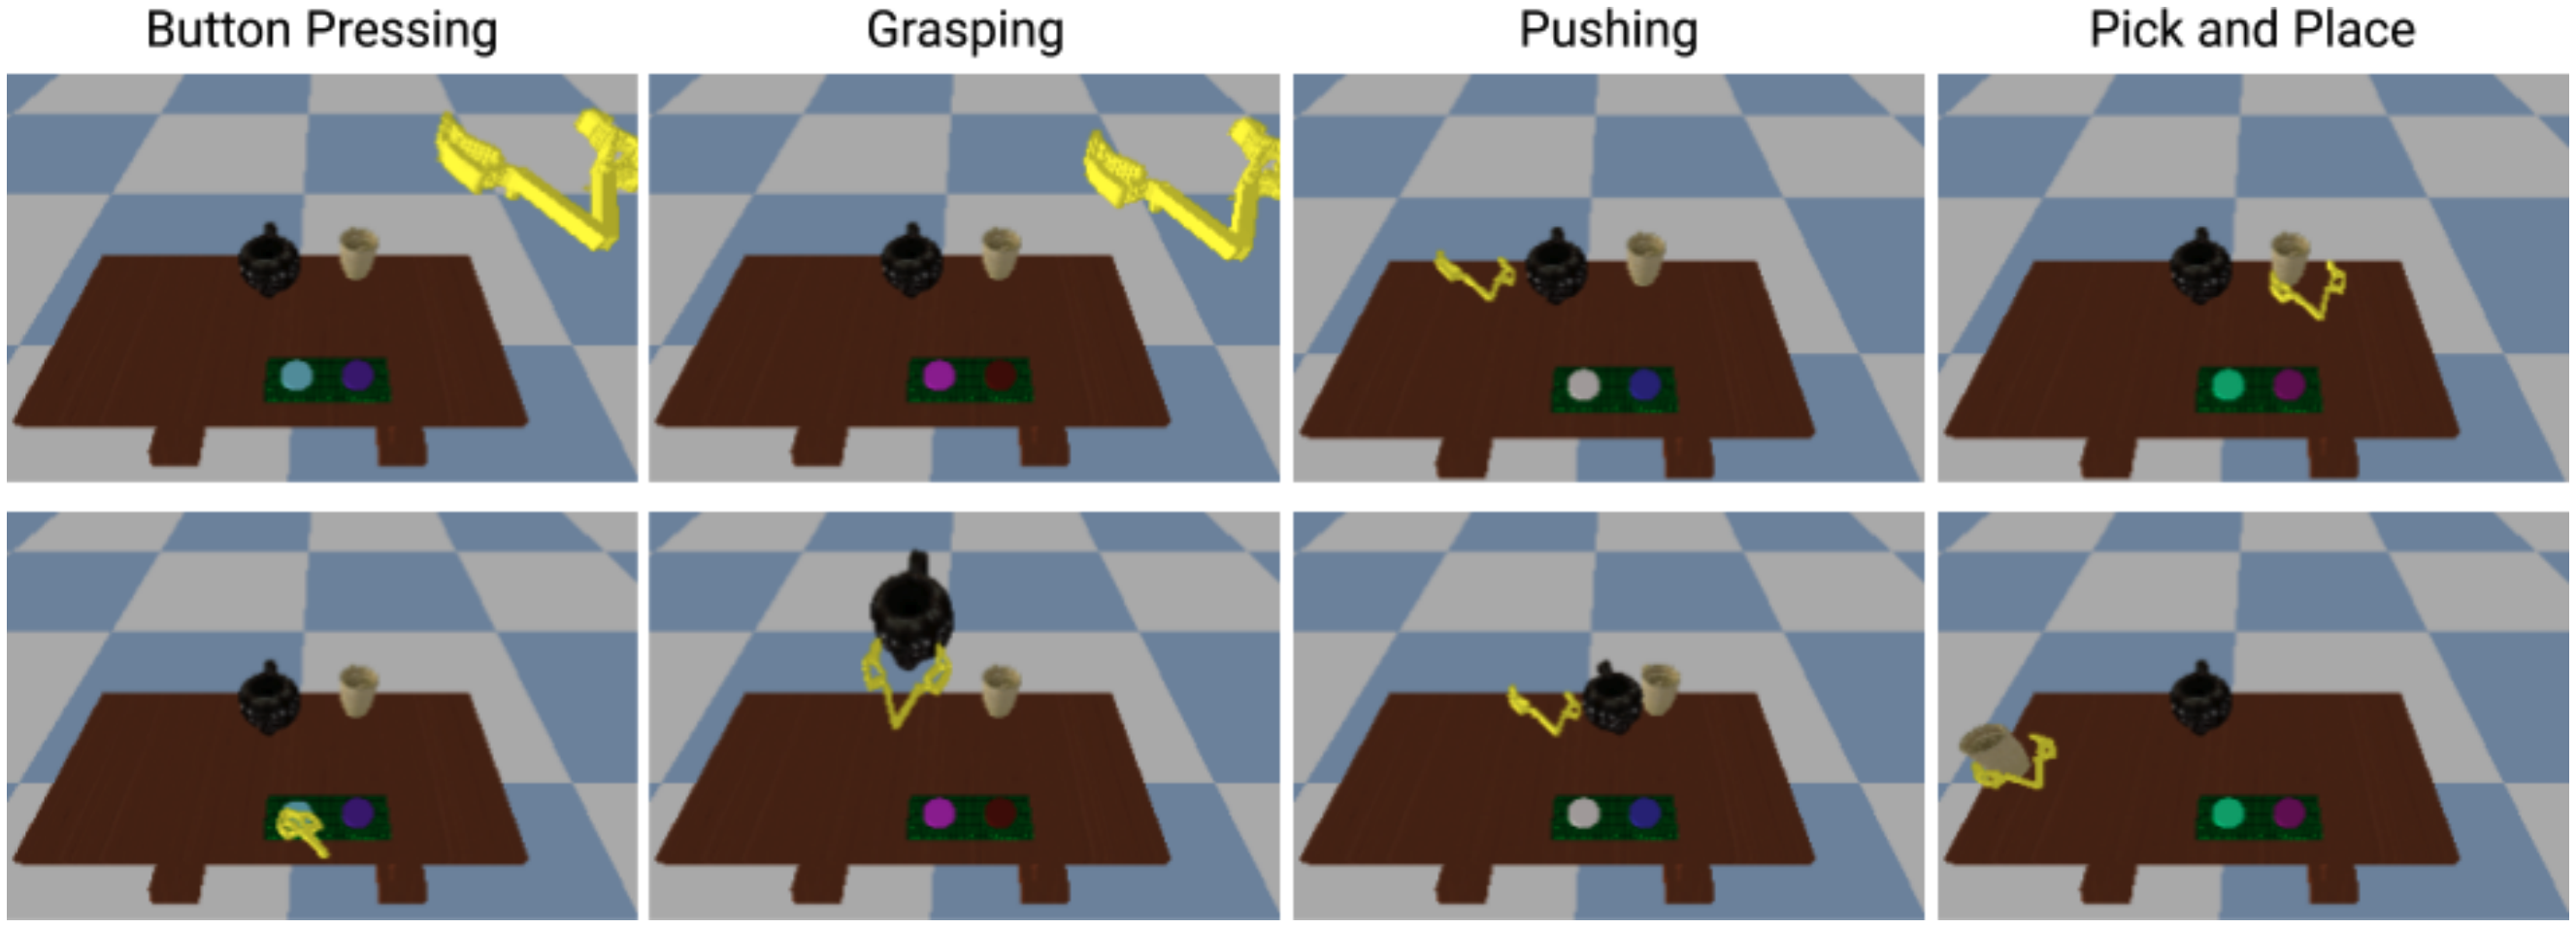
\includegraphics{src/Figures/watch-try-learn-envs.png}

}

\caption{\label{fig-envs}Visualization of different tasks from the
simulated benchmark for Watch Try Learn.}

\end{figure}%

Figure~\ref{fig-envs} illustrates the different task families considered
in the simulated Gripper environment. Button Pressing, Grasping,
Pushing, and Pick and Place. For each task family, the environment
supports hundreds of different tasks by changing the objects in the
scene and the objectives (e.g.~which object to pick and where to place).
For each task in each task family, a handful of expert demonstrations
are given in a demonstrations dataset. As mentioned previously, the
environment gives the agent image observations, and take in actions as
end-effector (gripper) positions, angles, and opening.

\textbf{Baselines:} The following three baselines are considered:

\begin{enumerate}
\def\labelenumi{\arabic{enumi}.}
\item
  \textbf{Behavior Cloning}: simple imitation learning based on maximum
  log-likelihood training using data from all tasks.
\item
  \textbf{Meta-imitation learning}: This baseline corresponds to simply
  running the policy from the Watch step, without using any trial data.
  That is, we only condition on the set of expert demonstrations, but no
  online trials.
\item
  \textbf{Behavior Cloning + SAC}: Pre-train a policy with Behavior
  Cloning on all data, and follow that with Reinforcement Learning
  fine-tuning for the specific target task, using the maximum-entropy
  algorithm SAC ((\citeproc{ref-haarnoja2018soft}{Haarnoja et al.
  2018})).
\end{enumerate}

\begin{figure}

\centering{

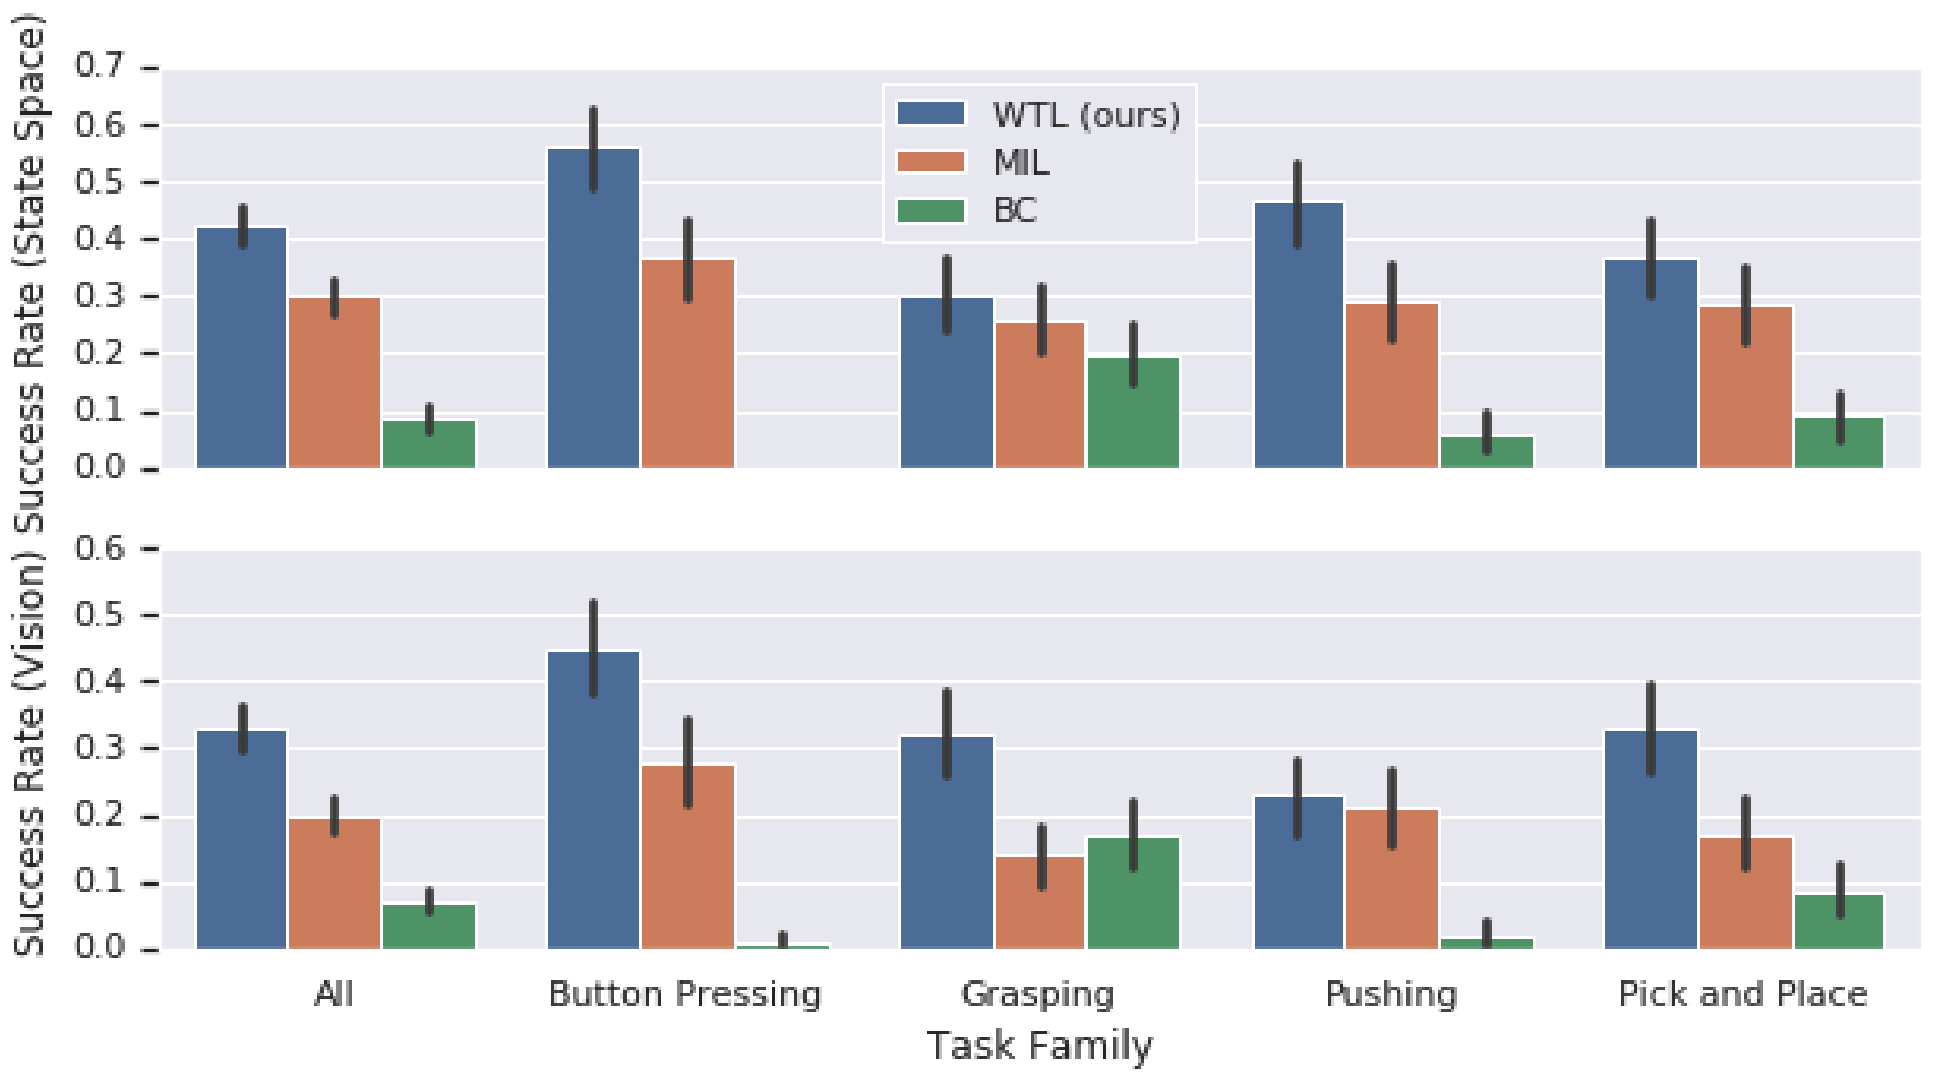
\includegraphics[width=0.5\textwidth,height=\textheight]{src/Figures/watch-try-learn-results.png}

}

\caption{\label{fig-watch-try-learn-results}Results for Watch Try Learn
on the gripper control environment, and comparisons with baselines.}

\end{figure}%

\begin{longtable}[]{@{}lc@{}}
\caption{Average success rates over all
tasks.}\label{tbl-watch-try-learn-table}\tabularnewline
\toprule\noalign{}
\textbf{METHOD} & \textbf{SUCCESS RATE} \\
\midrule\noalign{}
\endfirsthead
\toprule\noalign{}
\textbf{METHOD} & \textbf{SUCCESS RATE} \\
\midrule\noalign{}
\endhead
\bottomrule\noalign{}
\endlastfoot
BC & .09 \(\pm\) .01 \\
MIL & .30 \(\pm\) .02 \\
WTL, 1 TRIAL (OURS) & .42 \(\pm\) .02 \\
\textbf{RL FINE-TUNING WITH SAC} & \\
BC + SAC, 1500 TRIALS & .11 \(\pm\) .07 \\
BC + SAC, 2000 TRIALS & .29 \(\pm\) .10 \\
BC + SAC, 2500 TRIALS & .39 \(\pm\) .11 \\
\end{longtable}

Figure~\ref{fig-watch-try-learn-results} shows average success rates for
Watch Try Learn compared to baselines. Watch Try Learn significantly
outperforms baselines on every task family. In particular, it is far
superior to Behavior Cloning, which is a very weak baseline, and it
significantly surpasses Meta-Imitation Learning on 3 out of 4 task
families. Table~\ref{tbl-watch-try-learn-table} includes comparison with
BC fine-tuned with Reinforcement Learning. Even after 2500 online
trials, SAC is not able to obtain the success rate that Watch Try Learn
achieves after only 1 trial. Overall, Watch Try Learn exhibits very
significant performance gains over prior methods.

\subsection{Direct Preference
Optimization}\label{direct-preference-optimization}

A modern method for estimating the parameters of a human preference
model is direct preference optimization
(\citeproc{ref-rafailov2023direct}{Rafailov et al. 2023}), which is used
in the context of aligning language models to human preferences. A
recent approach (\citeproc{ref-christiano2023deep}{Christiano et al.
2023}) first trains a reward model that captures human preferences and
then uses proximal policy optimization to train a language model-based
policy to reflect those learned preferences. Direct Preference
Optimization (DPO), on the other hand, removes the need for a reward
model by directly using the model likelihood of two outcomes (a
preferred or highly-ranked sequence and an unpreferred or low-ranked
sequence) to capture the preference represented in the data. DPO
provides a simpler framework than its reinforcement learning approach
and results in comparable performance with improved stability.
Furthermore, it obviates the need to train a reward model, instead using
a language model policy and human preference dataset to align the policy
directly to human preferences.

\subsection{Model Design
Consideration}\label{model-design-consideration}

When designing models and learning their parameters, one must account
for important tradeoffs when designing and optimizing a model to learn
human preferences.

\textbf{Bias vs.~Variance Trade-off.} In modeling human preferences, we
aim to ensure that predicted utilities accurately reflect overall human
preferences. One key challenge is managing the bias and variance
trade-off.

Bias refers to assumptions made during model design and training that
can skew predictions. For example, in Ideal Point Models, we make the
assumption that the representations we use for individuals and choices
are aligned in the embedding space, and that this representation is
sufficient to capture human preferences using distance metrics. However,
there are myriad cases in which this may break down, for example if the
two sets of vectors follow different distributions each with their own
unique biases. If the representations do not come from the same domain,
one may have little visibility into how a distance metric computes the
final utility value for a choice for a given individual. Some ways to
mitigate bias in human preference models include increasing the number
of parameters in a model (allowing for better learning of patterns in
the data) or removing inductive biases based on our assumptions of the
underlying data.

On the other hand, variance refers to the model's sensitivity to small
changes in the input, which leads to significant changes in the outp ut.
This phenomenon is often termed `overfitting' or `overparameterization.'
This behavior can occur in models that have many parameters, and learn
correlations in the data that do not contribute to learning human
preferences, but are artifacts of noise in the dataset that one should
ultimately ignore. One can address variance in models by reducing the
number of parameters or incorporating biases in the model based on
factors we can assume about the data.

\textbf{Model Scope.} One important consideration unique to human
preference models is that we wish to model individual preferences, and
we may choose to do so at arbitrary granularity. For example, we can fit
models to a specific individual or even multiple models for an
individual, each for different purposes or contexts. On the other end of
the spectrum, we may create a model to capture human preferences across
large populations or the world.

Individual models may certainly prove to be more powerful, as they do
not need to generalize across multiple individuals and can dedicate all
of their parameters to learning the preferences of a single user. In the
context of human behavior, this can be a significant advantage as any
two individuals can be arbitrarily different or even opposite in their
preferences. On the other hand, models fit only one person can
tremendously overfit to the training distribution and capture noise in
the data, which is not truly representative of human preferences.

On the end of the spectrum, models fit to the entire world may be
inadequate to model human preferences for arbitrary individuals,
especially those whose data it has not been fit to. As such, models may
underfit the given training distribution. These models aim to generalize
to many people but may fail to capture the nuances of individual
preferences, especially for those whose data is not represented in the
training set. As a result, they may not perform well for arbitrary
individuals within the target population

Choosing the appropriate scope for a model is crucial. ne must balance
the trade-off between overfitting to noise in highly granular models and
underfitting in broader models that may not capture individual nuances.

\section{Multimodal Preferences}\label{multimodal-preferences}

One of the core assumptions about learning a reward function is that it
is unimodal, meaning that it consists of data from one person with a
certain set of preferences or a group of people with similar
preferences. However, the model of unimodality often oversimplifies
human preferences and their often conflicting nature. To accurately
capture all the nuances of human preference, we examine a multi-modal
distribution with some baseline assumptions. Consider a scenario where
we, as regular drivers, make a left-hand turn at an intersection
(\citeproc{ref-myers2021learning}{Myers et al. 2021}). What would we do
if we saw a car speeding down the road approaching us? The figure below
describes some options. Following a timid driving pattern, some vehicles
would stop to let the other car go, preventing a collision. Other
vehicles would be more aggressive and try to make the turn before
colliding with the oncoming vehicle. Given the data of one of these
driving patterns, our model (our autonomous vehicle) can make an
appropriate decision. However, what if our model was given data from
both aggressive and timid drivers, and we don't know which data
corresponds to which type of driver? If we applied standard learning
based on comparison techniques, we see, as illustrated by the figure
below, that the car would have an accident trying to find a policy close
enough to both driving patterns.

\begin{figure}

\centering{

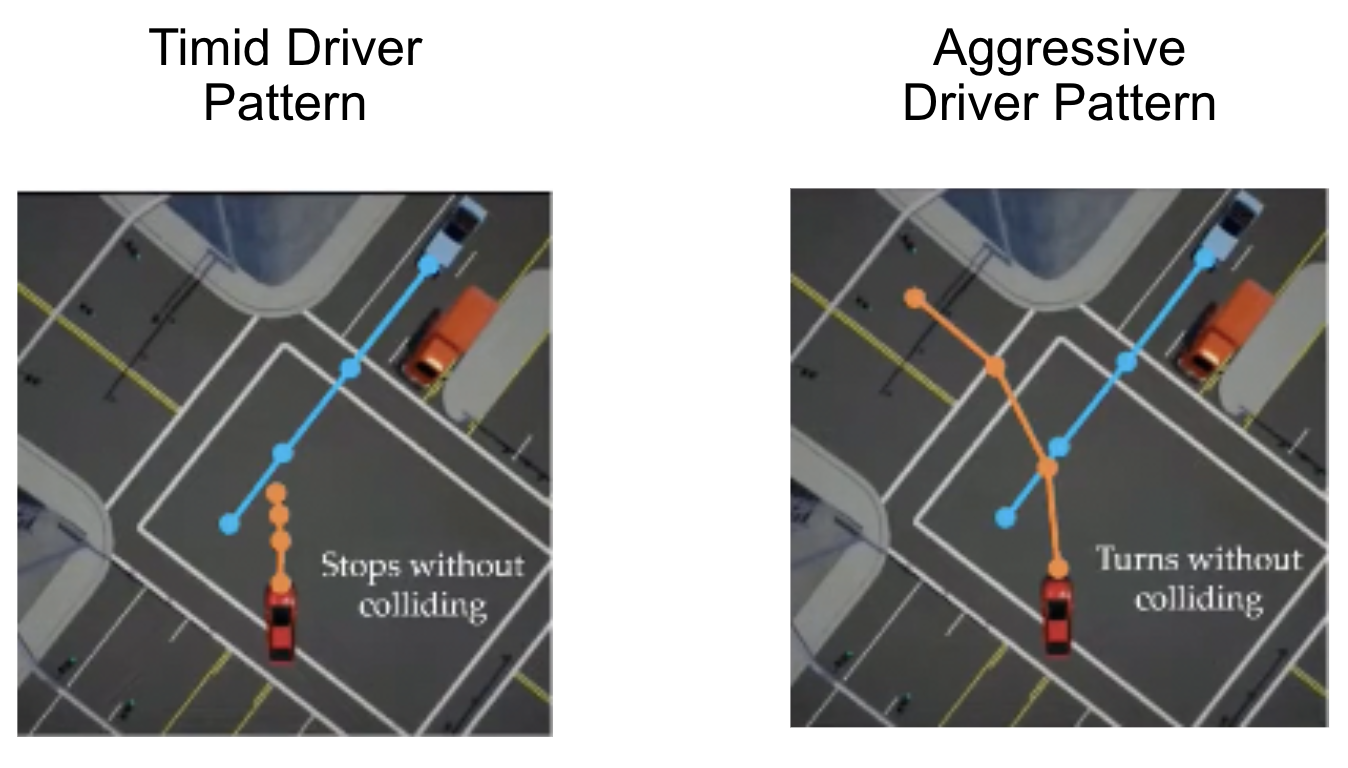
\includegraphics{src/Figures/driving-patt.png}

}

\caption{\label{fig-driving-patt}(\citeproc{ref-myers2021learning}{Myers
et al. 2021}) shows the possibilities of 2 different driving patterns
when a car is taking a left-hand turn at an intersection and sees
another car approaching head-on.}

\end{figure}%

\begin{figure}

\centering{

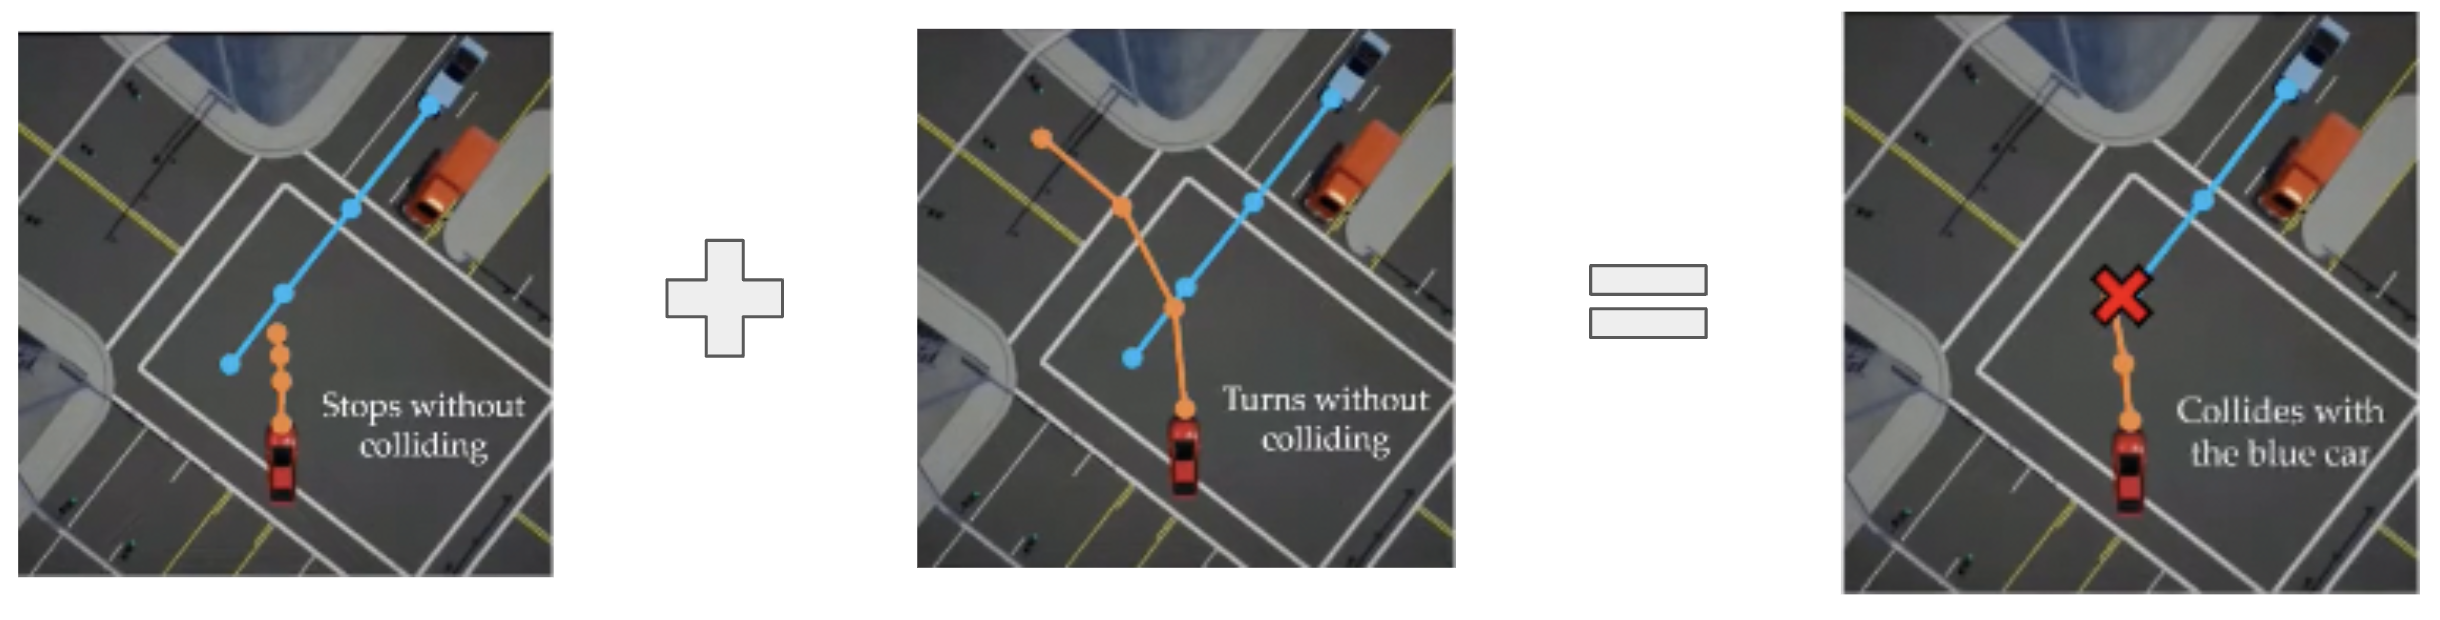
\includegraphics{src/Figures/driving-coll.png}

}

\caption{\label{fig-driving-coll}The figure
(\citeproc{ref-myers2021learning}{Myers et al. 2021}) depicts the
resultant collision when we try to find a policy close enough to both
the driving patterns.}

\end{figure}%

As illustrated by the driving example, we see that multi-modality for
our reward function is extremely important and, in some cases, if it is
not considered, can lead to fatal decisions
(\citeproc{ref-myers2021learning}{Myers et al. 2021}). But why can't we
label the groups, which would be the timid and aggressive drivers in the
driving case, and then learn separate reward functions for each driver?
The first problem with this approach is that it is inefficient and
time-consuming to separate the data into groups because we would have to
cluster and label the data. Secondly, it would not be accurate just to
split the data because a more timid driver can be aggressive when they
are in a hurry.

To formulate this problem of learning reward functions and mixing
coefficients from ranking queries in a fully observable deterministic
dynamical system, we begin by describing the system as a trajectory
\(\xi = (s_0, a_0, ..., s_T, a_T)\), where the sequence of states and
actions represents the system's evolution over time. Assume there are
\(M\) different reward functions, each representing an expert's
preferences. Using the linearity assumption in reward learning, we model
each expert's reward function as a linear combination of features in a
known, fixed feature space \(\phi(\xi)\). The reward for the \(m\)-th
expert is given by: \[R_m(\xi) = \omega^T_m \phi(\xi),\] where
\(\omega_m\) is a vector of parameters corresponding to the \(m\)-th
expert's preferences. There exists an unknown distribution over the
reward parameters and we can represent this distribution with mixing
coefficients \(\alpha_m\) such that \(\sum_M^{m = 1} \alpha_m = 1\). Our
goal is to learn reward functions and mixing coefficients using ranking
queries.

To define our problem, let's consider a robot who performs the following
trajectories and asks a user to rank all the trajectories.

\begin{figure}

\centering{

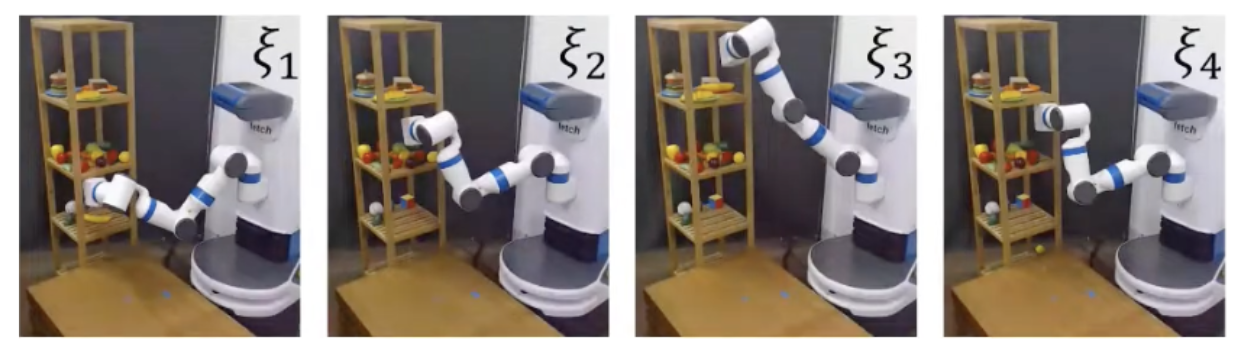
\includegraphics{src/Figures/robot-traj.png}

}

\caption{\label{fig-robot-traj}The figure
(\citeproc{ref-myers2022learning}{Myers et al. 2022}) depicts a few
different trajectories for an example multi-modal ranking scenario.}

\end{figure}%

The robot will be given back a set of trajectory rankings, coming from M
humans and the objective is to learn the underlying reward function. We
can represent the response of the ranking query as
\(x = (\xi_{a_1},\ ...\ ,\xi_{a_K})\) where \(a_1\) is the index of the
expert's top choice, \(a_2\) is the index of the expert's second choice,
... and so on. With the response \(x\), we generate a probability
distribution with the softmax rule
(\citeproc{ref-myers2022learning}{Myers et al. 2022}):
\(Pr(x_1 = \xi_{a_1} | R = R_m) = \frac{e^R_m(\xi_{a_1})}{\sum_{j=1}^Ke^R_m(\xi_{a_j})}\).
where \(R_m(\xi_{a_i})\) denotes the reward assigned by the \(m\)-th
expert to trajectory \(\xi_{a_i}\). Then, we randomly sample our
probability distribution to pick our top choice. From the remaining
trajectories, we noisily choose from our distribution to rank our
second-best option. We repeat this process until we have ranked all our
trajectories. This follows what is known as the Plackett-Luce Ranking
Model.

Given knowledge of the true reward function weights \(\omega_m\) and
mixing coefficients \(\alpha_m\), we have the following joint mass over
observations x from a query Q:
\(Pr(x\ |\ Q) = \sum_{m = 1}^M \alpha_m\prod_{i = 1}^K\frac{e^{\omega_m^T \Phi(\xi_{a_i})}}{\sum_{j = i}^K e^{\omega_m^T \Phi(\xi_{a_j})}}\).

With the above formulation of the joint mass distribution over
observation and queries, we can now formulate an objective.
Specifically, it is to present users with the best set of queries that
learn reward weights, \(\omega\), and mixing coefficient, \(\alpha\),
based upon user rankings of preferred query responses. By learning these
parameters, we can have an accurate estimation of the joint mass
distribution of the observations.

To learn these parameters, we use a Bayesian learning framework. The
goal will be to learn the reward weights, \(\omega_m\), and all mixing
coefficients \(\alpha_m\). Thus, define the parameters to be
\(\theta = \{\omega, \alpha\}\). We start by simplifying the posterior
over the parameters.

\[\begin{aligned}
\Pr(\Theta | Q^{(1)}, x^{(1)}, Q^{(2)}, x^{(2)}, \ldots) & \propto \Pr(\Theta) \Pr(Q^{(1)} | x^{(1)}, Q^{(2)}, x^{(2)}, \ldots | \Theta) \\
& = \Pr(\Theta) \prod_t \Pr(x^{(t)} | Q^{(t)}, \Theta, Q^{(1)}, x^{(1)}, \ldots, Q^{(t-1)}, x^{(t-1)}) \\
& \propto \Pr(\Theta) \prod_t \Pr(x^{(t)} | \Theta, Q^{(t)})
\end{aligned}\]

Note that the first proportionality term is directly from Bayes rule
(removing normalization constant). The first equation comes directly
from the assumption that the queries at timestamp \(t\) are
conditionally independent of the parameters given previous queries \&
rankings. This assumption is reasonable because the previous queries \&
rankings ideally give all the information to inform the choice of the
next set of. The last proportionality term comes from the assumption
that the ranked queries are conditionally independent given the
parameters

The prior distribution is dependent on use case. For example, in the
user studies conducted by the authors to verify this method, they use a
standard Gaussian for the reward weights and the mixing coefficients to
be uniform on a \(M - 1\) simplex to ensure that they add up to 1. Then
we can use maximum likelihood estimation to compute the parameters with
the simplified posterior.

\section{Social Choices}\label{social-choices}

Game theory provides a mathematical framework for analyzing strategic
interactions among rational agents. These models help in understanding
and predicting human behavior by considering multiple criteria and the
associated trade-offs. They enhance the understanding of preferences
across multiple criteria and allow for richer and more accurate feedback
through structured comparisons. Game-theory framings capture the
complexity of preferences and interactions in decision-making processes
(\citeproc{ref-bhatia2020preference}{Bhatia et al. 2020}).

The most popular form of preference elicitation involves pairwise
comparisons. Users are asked to choose between two options, such as
product A or product B. This method is used in various applications like
search engines, recommender systems, and interactive robotics. Key
concepts include the Von Neumann Winner and the Blackwell Winner. The
Von Neumann Winner refers to a distribution over objects that beats or
ties every other object in the collection under the expected utility
assumption. The Blackwell Winner generalizes the Von Neumann Winner for
multi-criteria problems using a target set for acceptable payoff vectors
(\citeproc{ref-bhatia2020preference}{Bhatia et al. 2020}).

Game-theory framings provide a framework for preference learning along
multiple criteria. These models use tools from vector-valued payoffs in
game theory, with Blackwell's approach being a key concept. This
approach allows for a more comprehensive understanding of preferences by
considering multiple criteria simultaneously
(\citeproc{ref-bhatia2020preference}{Bhatia et al. 2020}).

In game-theory framings, pairwise preferences are modeled as random
variables. Comparisons between objects along different criteria are
captured in a preference tensor \(P\). This tensor models the
probability that one object is preferred over another along a specific
criterion, allowing for a detailed understanding of preferences across
multiple dimensions (\citeproc{ref-bhatia2020preference}{Bhatia et al.
2020}).

The preference tensor \(P\) captures object comparisons along different
criteria. It is defined as:
\[P(i_1, i_2; j) = P(i_1 \succ i_2 \text{ along criterion } j)\] where
\(P(i_2, i_1; j) = 1 - P(i_1, i_2; j)\). These values are aggregated to
form an overall preference matrix \(P_{ov}\)
(\citeproc{ref-bhatia2020preference}{Bhatia et al. 2020}).

The Blackwell Winner is defined using a target set \(S\) of acceptable
score vectors. The goal is to find a distribution \(\pi^*\) such that
\(P(\pi^*, \pi) \in S\) for all \(\pi\). This method minimizes the
maximum distance to the target set, providing a robust solution to
multi-criteria preference problems
(\citeproc{ref-bhatia2020preference}{Bhatia et al. 2020}).

The optimization problem for finding the Blackwell Winner is defined as:
\[\pi(P, S, \|\cdot\|) = \arg \min_{\pi \in \Delta_d} \left[ \max_{\pi' \in \Delta_d} \rho(P(\pi, \pi'), S) \right]\]
where \(\rho(u, v) = \|u - v\|\). This measures the distance to the
target set, ensuring that the selected distribution is as close as
possible to the ideal preference vector
(\citeproc{ref-bhatia2020preference}{Bhatia et al. 2020}).

\section{Exercises}\label{exercises}

\subsection*{Question 1: Choice Modeling (15
points)}\label{question-1-choice-modeling-15-points}
\addcontentsline{toc}{subsection}{Question 1: Choice Modeling (15
points)}

In Chapter 2, we discussed discrete choice modeling in the context of
utility being a linear function. Suppose we are deciding between \(N\)
choices and that the utility of each choice is given by
\(U_i=\beta_i\mathbf{x}+\epsilon_i\) for \(i=1, 2, \cdots, N\). We view
\(\mathbf{x}\) as the data point that is being conditioned on for
deciding which choice to select, and \(\beta_i\) as the weights driving
the linear utility model. The noise \(\epsilon_i\) is i.i.d. sampled
from a type of extreme value distribution called the \emph{Gumbel}
distribution. The standard Gumbel distribution is given by the density
function \(f(x)=e^{-(x+e^{-x})}\) and cumulative distribution function
\(F(x)=e^{-e^{-x}}.\) Fix \(i\). Our objective is to calculate
\(\Pr(U_i\,\, \text{has max utility})\).

\begin{enumerate}
\def\labelenumi{(\alph{enumi})}
\item
  \textbf{(Written, 2 points)}. To start, set \(U_i=t\) and compute
  \(\Pr(U_j<t)\) for \(j\neq i\) in terms of \(F\). Use this probability
  to derive an integral for \(\Pr(U_i\,\,  \text{has max utility})\)
  over \(t\) in terms of \(f\) and \(F\).

  Example of solution environment.
\item
  \textbf{(Written, 4 points)}. Compute the integral derived in part (a)
  with the appropriate \(u\)-substitution. Show your work. You should
  arrive at multi-class logistic regression in the end!
\end{enumerate}

Next, you will implement logistic regression to predict preferred prompt
completions. We will use the preference dataset from
\href{https://huggingface.co/datasets/allenai/reward-bench}{RewardBench}.
Notice the provided \texttt{data/chosen\_embeddings.pt} and
\texttt{data/rejected\_embeddings.pt} files. These files were
constructed by feeding the prompt alongside the chosen/rejected
responses through Llama3-8B-Instruct and selecting the last token's
final hidden embedding. Let \(e_1\) and \(e_2\) be two hidden embeddings
with \(e_1\succ e_2\). We assume weights \(w\) exist for which the
Bradley-Terry reward of an embedding \(e\) can be modeled as
\(r=w\cdot e\). In this setting, the probability of \(e_1\succ e_2\) is
\[\frac{e^{w\cdot e_1}}{e^{w\cdot e_1}+e^{w\cdot e_2}}=\frac{1}{1+e^{w\cdot(e_2-e_1)}}=\sigma(w\cdot(e_1-e_2)).\]
Hence, we can view maximum likelihood across the preference dataset with
this model as logistic regression on \(e_1-e_2\) without a bias term and
all labels being \(1\).

In biasless logistic regression, we are given a dataset \(X\) with \(N\)
rows of datapoints and \(D\) features per datapoint. The weights of the
model are parametrized by \(\theta\), a \(D\)-dimensional column vector.
Given binary labels \(y\) of shape \(N\) by \(1\), the binary
cross-entropy loss is
\[J(\theta)=-\frac{1}{N}(y^T\log(\sigma(X\theta)) + (1-y)^T\log(1-\sigma(X\theta)))\]
where \(\sigma\) is the sigmoid function and is applied element-wise
along with \(\log\). The gradient of loss is
\[\nabla_\theta J(\theta)=\frac{1}{N}X^T(\sigma(X\theta)-y).\]

\begin{enumerate}
\def\labelenumi{\arabic{enumi}.}
\item
  \textbf{(Coding, 3 points)}. Open the file
  \texttt{logistic\_regression/logistic\_regression.py}. Implement the
  function \texttt{train} in the biasless case.
\item
  \textbf{(Coding, 2 points)}. Implement the function
  \texttt{predict\_probs}.
\item
  \textbf{(Written, 4 points)}. Open the notebook
  \texttt{rewardbench\_preferences.ipynb} and run all the cells. Make
  sure to tune the \texttt{learning\_rate} and \texttt{num\_iterations}.
  Report your final expected accuracy on the training and validation
  sets. How close are the two expected accuracies? You should be able to
  achieve \(\approx 90\%\) expected accuracy on validation. You may add
  loss reporting to the \texttt{train} function to verify your model is
  improving over time.
\end{enumerate}

\begin{Shaded}
\begin{Highlighting}[numbers=left,,]
\ImportTok{from}\NormalTok{ sklearn.model\_selection }\ImportTok{import}\NormalTok{ train\_test\_split}
\ImportTok{import}\NormalTok{ torch}

\KeywordTok{class}\NormalTok{ LogisticRegression:}
    \KeywordTok{def} \FunctionTok{\_\_init\_\_}\NormalTok{(}\VariableTok{self}\NormalTok{):}
        \VariableTok{self}\NormalTok{.weights }\OperatorTok{=} \VariableTok{None}  \CommentTok{\# Initialized during training}

    \KeywordTok{def}\NormalTok{ train(}\VariableTok{self}\NormalTok{, X, y, learning\_rate, num\_iterations):}
        \CommentTok{"""}
\CommentTok{        Train the logistic regression model using gradient descent (no bias).}
\CommentTok{        Each gradient update should be with respect to the entire dataset X.}

\CommentTok{        Parameters:}
\CommentTok{        {-} X (torch.Tensor): Training data of shape (n\_samples, n\_features).}
\CommentTok{        {-} y (torch.Tensor): Target labels of shape (n\_samples,).}
\CommentTok{        """}
\NormalTok{        n\_samples, n\_features }\OperatorTok{=}\NormalTok{ X.shape}

        \CommentTok{\# Initialize weights without the bias term}
        \VariableTok{self}\NormalTok{.weights }\OperatorTok{=}\NormalTok{ torch.zeros(n\_features)}

        \ControlFlowTok{for}\NormalTok{ i }\KeywordTok{in} \BuiltInTok{range}\NormalTok{(num\_iterations):}
            \CommentTok{\# YOUR CODE HERE (\textasciitilde{}4{-}5 lines)}
                \ControlFlowTok{pass}
            \CommentTok{\# }\RegionMarkerTok{END}\CommentTok{ OF YOUR CODE}

    \KeywordTok{def}\NormalTok{ predict\_probs(}\VariableTok{self}\NormalTok{, X):}
        \CommentTok{"""}
\CommentTok{        Predict probabilities for samples in X (no bias).}

\CommentTok{        Parameters:}
\CommentTok{        {-} X (torch.Tensor): Input data of shape (n\_samples, n\_features).}

\CommentTok{        Returns:}
\CommentTok{        {-} y\_probs (torch.Tensor): Predicted probabilities.}
\CommentTok{        """}
\NormalTok{        y\_probs }\OperatorTok{=} \VariableTok{None}

        \CommentTok{\# YOUR CODE HERE (\textasciitilde{}2{-}3 lines)}
        \ControlFlowTok{pass}
        \CommentTok{\# }\RegionMarkerTok{END}\CommentTok{ OF YOUR CODE}

        \ControlFlowTok{return}\NormalTok{ y\_probs}


\ControlFlowTok{if} \VariableTok{\_\_name\_\_} \OperatorTok{==} \StringTok{"\_\_main\_\_"}\NormalTok{:}
    \CommentTok{\# \%\%}
    \CommentTok{\# Load in Llama3 embeddings of prompt + completions on RewardBench}
\NormalTok{    chosen\_embeddings }\OperatorTok{=}\NormalTok{ torch.load(}\StringTok{\textquotesingle{}data/chosen\_embeddings.pt\textquotesingle{}}\NormalTok{)}
\NormalTok{    rejected\_embeddings }\OperatorTok{=}\NormalTok{ torch.load(}\StringTok{\textquotesingle{}data/rejected\_embeddings.pt\textquotesingle{}}\NormalTok{)}

    \CommentTok{\# Subtract the embeddings according to the Bradley{-}Terry reward model setup presented in the problem }
\NormalTok{    X }\OperatorTok{=}\NormalTok{ (chosen\_embeddings }\OperatorTok{{-}}\NormalTok{ rejected\_embeddings).to(torch.}\BuiltInTok{float}\NormalTok{)}
\NormalTok{    y }\OperatorTok{=}\NormalTok{ torch.ones(X.shape[}\DecValTok{0}\NormalTok{])}

    \CommentTok{\# Split dataset 80/20 into training and validation sets}
\NormalTok{    X\_train, X\_val, y\_train, y\_val }\OperatorTok{=}\NormalTok{ train\_test\_split(X, y, test\_size}\OperatorTok{=}\FloatTok{0.2}\NormalTok{, random\_state}\OperatorTok{=}\DecValTok{42}\NormalTok{)  }

    \BuiltInTok{print}\NormalTok{(}\StringTok{"Training set size:"}\NormalTok{, X\_train.shape)}
    \BuiltInTok{print}\NormalTok{(}\StringTok{"Validation set size:"}\NormalTok{, X\_val.shape)}

\NormalTok{    model }\OperatorTok{=}\NormalTok{ LogisticRegression()}

    \CommentTok{\# Tune the learning\_rate and num\_iterations until you achieve expected validation accuracy of at least 90\%}
\NormalTok{    learning\_rate }\OperatorTok{=} \VariableTok{None}
\NormalTok{    num\_iterations }\OperatorTok{=} \VariableTok{None}

\NormalTok{    model.train(X\_train, y\_train, learning\_rate}\OperatorTok{=}\NormalTok{learning\_rate, num\_iterations}\OperatorTok{=}\NormalTok{num\_iterations)}

\NormalTok{    y\_train\_probs }\OperatorTok{=}\NormalTok{ model.predict\_probs(X\_train)}
    \BuiltInTok{print}\NormalTok{(}\SpecialStringTok{f"Expected Train Accuracy: }\SpecialCharTok{\{}\NormalTok{y\_train\_probs}\SpecialCharTok{.}\NormalTok{mean()}\SpecialCharTok{\}}\SpecialStringTok{"}\NormalTok{)}

\NormalTok{    y\_val\_probs }\OperatorTok{=}\NormalTok{ model.predict\_probs(X\_val)}
    \BuiltInTok{print}\NormalTok{(}\SpecialStringTok{f"Expected Validation Accuracy: }\SpecialCharTok{\{}\NormalTok{y\_val\_probs}\SpecialCharTok{.}\NormalTok{mean()}\SpecialCharTok{\}}\SpecialStringTok{"}\NormalTok{) }\CommentTok{\# Should reach at least 90\%}
\end{Highlighting}
\end{Shaded}

\subsection*{Question 2: Revealed and Stated Preferences (20
points)}\label{question-2-revealed-and-stated-preferences-20-points}
\addcontentsline{toc}{subsection}{Question 2: Revealed and Stated
Preferences (20 points)}

Alice and Bob are running for president. For \(R\) voters, we have
access to their revealed candidate preferences through some means (e.g.,
social media, blogs, event history). Assume there is an underlying
probability \(z\) of voting for Alice among the population that is
unknown. The aim of this question is to estimate \(z\) through
\emph{maximum likelihood estimation} by also incorporating stated
preferences. In this scenario, we collect stated preferences through
surveys. When surveyed, voters tend to be more likely to vote for Alice
with probability \(\frac{z+1}{2}\) for reasons of ``political
correctness.''

\begin{enumerate}
\def\labelenumi{(\alph{enumi})}
\item
  \textbf{(Written, 5 points)}. Suppose there are \(R_A\) revealed
  preferences for Alice, \(R_B\) revealed preferences for Bob, \(S_A\)
  stated preferences for Alice, and \(S_B\) stated preferences for Bob.
  Note \(R=R_A+R_B\). Compute the log-likelihood of observing such
  preferences in terms of \(z, R_A, R_B, S_A, S_B\).
\item
  \textbf{(Coding, 1 point)}. Implement the short function
  \texttt{stated\_prob} in the file \texttt{voting/simulation.py}.
\item
  \textbf{(Coding, 5 points)}. Implement the class
  \texttt{VotingSimulation}.
\item
  \textbf{(Coding, 7 points)}. Implement your derived expression from
  part (a) in the \texttt{log\_likelihoods} function.
\item
  \textbf{(Written, 2 points)}. Finally, implement the
  \texttt{average\_mae\_mle} method that will allow us to visualize the
  mean absolute error (MAE) of our maximum likelihood estimate
  \(\hat{z}\) (i.e., \(|\hat{z}-z|\)) as the number of voters surveyed
  increases. Open \texttt{voting/visualize\_sim.ipynb} and run the cells
  to get a plot of MAE vs.~voters surveyed averaged across \(100\)
  simulations. Attach the plot to this question and briefly explain what
  you notice.
\end{enumerate}

\begin{Shaded}
\begin{Highlighting}[numbers=left,,]
\ImportTok{import}\NormalTok{ torch}
\ImportTok{import}\NormalTok{ random}
\ImportTok{import}\NormalTok{ matplotlib.pyplot }\ImportTok{as}\NormalTok{ plt}
\ImportTok{from}\NormalTok{ tqdm }\ImportTok{import}\NormalTok{ tqdm}
\NormalTok{random.seed(}\DecValTok{42}\NormalTok{)}
\NormalTok{torch.manual\_seed(}\DecValTok{42}\NormalTok{)}

\KeywordTok{def}\NormalTok{ stated\_prob(z\_values):}
    \CommentTok{"""}
\CommentTok{    Computes the probability of stated preferences based on z values.}
\CommentTok{    }
\CommentTok{    Args:}
\CommentTok{        z\_values (torch.Tensor): The z value(s), where z represents the true probability of voting for Alice.}

\CommentTok{    Returns:}
\CommentTok{        torch.Tensor: Probability for stated preferences, derived from z values.}
\CommentTok{    """}
    \CommentTok{\# YOUR CODE HERE (\textasciitilde{}1 line)}
    \CommentTok{\# }\RegionMarkerTok{END}\CommentTok{ OF YOUR CODE}

\KeywordTok{class}\NormalTok{ VotingSimulation:}
    \CommentTok{"""}
\CommentTok{    A class to simulate the voting process where revealed and stated preferences are generated.}
\CommentTok{    }
\CommentTok{    Attributes:}
\CommentTok{        R (int): Number of revealed preferences.}
\CommentTok{        z (float): The true probability of voting for Alice.}
\CommentTok{        revealed\_preferences (torch.Tensor): Simulated revealed preferences of R voters using Bernoulli distribution.}
\CommentTok{                                             Takes on 1 for Alice, and 0 for Bob.}
\CommentTok{        stated\_preferences (torch.Tensor): Simulated stated preferences, initialized as an empty tensor.}
\CommentTok{                                           Takes on 1 for Alice, and 0 for Bob.}
\CommentTok{    """}
    \KeywordTok{def} \FunctionTok{\_\_init\_\_}\NormalTok{(}\VariableTok{self}\NormalTok{, R, z):}
        \VariableTok{self}\NormalTok{.R }\OperatorTok{=}\NormalTok{ R}
        \VariableTok{self}\NormalTok{.z }\OperatorTok{=}\NormalTok{ z}
        \VariableTok{self}\NormalTok{.revealed\_preferences }\OperatorTok{=} \VariableTok{None} \CommentTok{\# YOUR CODE HERE (\textasciitilde{}1 line)}
        \VariableTok{self}\NormalTok{.stated\_preferences }\OperatorTok{=}\NormalTok{ torch.tensor([])}

    \KeywordTok{def}\NormalTok{ add\_survey(}\VariableTok{self}\NormalTok{):}
        \CommentTok{"""}
\CommentTok{        Simulates an additional stated preference based on stated\_prob and adds it to the list.}
\CommentTok{        This updates the self.stated\_preferences tensor by concatenating on a new simulated survey result.}
\CommentTok{        """}
        \CommentTok{\# YOUR CODE HERE (\textasciitilde{}3 lines)}
        \CommentTok{\# }\RegionMarkerTok{END}\CommentTok{ OF YOUR CODE}

\KeywordTok{def}\NormalTok{ log\_likelihoods(revealed\_preferences, stated\_preferences, z\_values):}
    \CommentTok{"""}
\CommentTok{    Computes the log likelihoods across both revealed and stated preferences.}
\CommentTok{    Use your answer in part (a) to help.}
\CommentTok{    }
\CommentTok{    Args:}
\CommentTok{        revealed\_preferences (torch.Tensor): Tensor containing revealed preferences (0 or 1).}
\CommentTok{        stated\_preferences (torch.Tensor): Tensor containing stated preferences (0 or 1).}
\CommentTok{        z\_values (torch.Tensor): Tensor of underlying z values to calculate likelihood for.}

\CommentTok{    Returns:}
\CommentTok{        torch.Tensor: Log likelihood for each z value.}
\CommentTok{    """}
    \CommentTok{\# YOUR CODE HERE (\textasciitilde{}10{-}16 lines)}
    \ControlFlowTok{pass}
    \CommentTok{\# }\RegionMarkerTok{END}\CommentTok{ OF YOUR CODE }

\KeywordTok{def}\NormalTok{ average\_mae\_mle(R, z, survey\_count, num\_sims, z\_sweep):}
    \CommentTok{"""}
\CommentTok{    Runs multiple simulations to compute the average mean absolute error (MAE) of Maximum Likelihood Estimation (MLE) }
\CommentTok{    for z after increasing number of surveys.}
\CommentTok{    }
\CommentTok{    Args:}
\CommentTok{        R (int): Number of revealed preferences.}
\CommentTok{        z (float): The true probability of voting for Alice.}
\CommentTok{        survey\_count (int): Number of additional surveys to perform.}
\CommentTok{        num\_sims (int): Number of simulation runs to average over.}
\CommentTok{        z\_sweep (torch.Tensor): Range of z values to consider for maximum likelihood estimation.}

\CommentTok{    Returns:}
\CommentTok{        torch.Tensor: Tensor of mean absolute errors averaged over simulations.}
\CommentTok{                      Should have shape (survey\_count, )}
\CommentTok{    """}
\NormalTok{    all\_errors }\OperatorTok{=}\NormalTok{ []}
    \ControlFlowTok{for}\NormalTok{ \_ }\KeywordTok{in}\NormalTok{ tqdm(}\BuiltInTok{range}\NormalTok{(num\_sims)):}
\NormalTok{        errors }\OperatorTok{=}\NormalTok{ []}
\NormalTok{        vote\_simulator }\OperatorTok{=}\NormalTok{ VotingSimulation(R}\OperatorTok{=}\NormalTok{R, z}\OperatorTok{=}\NormalTok{z)}

        \ControlFlowTok{for}\NormalTok{ \_ }\KeywordTok{in} \BuiltInTok{range}\NormalTok{(survey\_count):}
\NormalTok{            revealed\_preferences }\OperatorTok{=}\NormalTok{ vote\_simulator.revealed\_preferences}
\NormalTok{            stated\_preferences }\OperatorTok{=}\NormalTok{ vote\_simulator.stated\_preferences}

            \CommentTok{\# YOUR CODE HERE (\textasciitilde{}6{-}8 lines)}
            \ControlFlowTok{pass} \CommentTok{\# Compute log\_likelihoods across z\_sweep. Argmax to find MLE for z. }
                 \CommentTok{\# Append the absolute error to errors and add a survey to the simulator.}
            \CommentTok{\# }\RegionMarkerTok{END}\CommentTok{ OF YOUR CODE}

\NormalTok{        errors\_tensor }\OperatorTok{=}\NormalTok{ torch.stack(errors) }
\NormalTok{        all\_errors.append(errors\_tensor)}

    \CommentTok{\# Calculate the average error across simulations }
\NormalTok{    mean\_errors }\OperatorTok{=}\NormalTok{ torch.stack(all\_errors).mean(dim}\OperatorTok{=}\DecValTok{0}\NormalTok{)}
    \ControlFlowTok{return}\NormalTok{ mean\_errors}

\ControlFlowTok{if} \VariableTok{\_\_name\_\_} \OperatorTok{==} \StringTok{"\_\_main\_\_"}\NormalTok{:}
    \CommentTok{\# DO NOT CHANGE!}
\NormalTok{    max\_surveys }\OperatorTok{=} \DecValTok{2000}
\NormalTok{    z }\OperatorTok{=} \FloatTok{0.5}
\NormalTok{    R }\OperatorTok{=} \DecValTok{10}
\NormalTok{    num\_sims }\OperatorTok{=} \DecValTok{100}
\NormalTok{    z\_sweep }\OperatorTok{=}\NormalTok{ torch.linspace(}\FloatTok{0.01}\NormalTok{, }\FloatTok{0.99}\NormalTok{, }\DecValTok{981}\NormalTok{)}

    \CommentTok{\# Compute and plot the errors. Attach this plot to part (d).}
\NormalTok{    mean\_errors }\OperatorTok{=}\NormalTok{ average\_mae\_mle(R, z, max\_surveys, num\_sims, z\_sweep)}
\NormalTok{    plt.plot(mean\_errors)}

\NormalTok{    plt.xlabel(}\StringTok{\textquotesingle{}Surveys Conducted\textquotesingle{}}\NormalTok{)}
\NormalTok{    plt.ylabel(}\StringTok{\textquotesingle{}Average Error\textquotesingle{}}\NormalTok{)}
\NormalTok{    plt.title(}\SpecialStringTok{f\textquotesingle{}MLE MAE Error (z=}\SpecialCharTok{\{}\NormalTok{z}\SpecialCharTok{\}}\SpecialStringTok{, }\SpecialCharTok{\{}\NormalTok{num\_sims}\SpecialCharTok{\}}\SpecialStringTok{ simulations)\textquotesingle{}}\NormalTok{)}
\NormalTok{    plt.show()}
\end{Highlighting}
\end{Shaded}

\subsection*{Question 3: Probabilistic Multi-modal Preferences (25
points)}\label{question-3-probabilistic-multi-modal-preferences-25-points}
\addcontentsline{toc}{subsection}{Question 3: Probabilistic Multi-modal
Preferences (25 points)}

Suppose you are part of the ML team on the movie streaming site
CardinalStreams. After taking CS329H, you collect a movie preferences
dataset with \(30000\) examples of the form
\((m_1, m_2, \text{user id})\) where \(m_1\) and \(m_2\) are movies with
\(m_1\succ m_2\). The preferences come from \(600\) distinct users with
\(50\) examples per user. Each movie has a \(10\)-dimensional feature
vector \(m\), and each user has a \(10\)-dimensional weight vector
\(u\). Given movie features \(m_1, m_2\) and user weights \(u\), the
user's preference between the movies is given by a Bradley-Terry reward
model, i.e.,
\[P(m_1\succ m_2)=\frac{e^{u\cdot m_1}}{e^{u\cdot m_1} + e^{u\cdot m_2}}=\frac{1}{1+e^{u\cdot (m_2-m_1)}}=\sigma(u\cdot (m_1-m_2)).\]

You realize that trying to estimate the weights for each user with only
\(50\) examples will not work due to the lack of data. Instead, you
choose to drop the user IDs column and shuffle the dataset in order to
take a \emph{multi-modal preferences} approach. For simplicity, you
assume a model where a proportion \(p\) of the users have weights
\(w_1\) and the other \(1-p\) have weights \(w_2\). In this setting,
each user belongs to one of two groups: users with weights \(w_1\) are
part of Group 1, and users with weights \(w_2\) are part of Group 2.

\begin{enumerate}
\def\labelenumi{(\alph{enumi})}
\item
  \textbf{(Written, 3 points)}. For a datapoint \((m_1, m_2)\) with
  label \(m_1\succ m_2\), compute the data likelihood
  \(P(m_1\succ m_2 | p, w_1, w_2)\) assuming \(p, w_1, w_2\) are given.
\item
  \textbf{(Written, 3 points)}. As a follow up, use the likelihood to
  simplify the posterior distribution of \(p, w_1, w_2\) after updating
  on \((m_1, m_2)\) leaving terms for the priors unchanged.
\item
  \textbf{(Written, 4 points)}. Assume priors \(p\sim B(1, 1)\),
  \(w_1\sim\mathcal{N}(0, \mathbf{I})\), and
  \(w_2\sim\mathcal{N}(0, \mathbf{I})\) where \(B\) represents the Beta
  distribution and \(\mathcal{N}\) represents the normal distribution.
  You will notice that the posterior from part (b) has no simple
  closed-form. As a result, we must resort to \emph{Markov Chain Monte
  Carlo (MCMC)} approaches to sample from the posterior. These
  approaches allow sampling from highly complex distributions by
  constructing a Markov chain \(\{x_t\}_{t=1}^\infty\) so that
  \(\lim_{t\to\infty}x_t\) act as desired samples from the target
  distribution. You can think of a Markov chain as a sequence with the
  special property that \(x_{t+1}\) only depends on \(x_t\) for all
  \(t\ge 1\).

  The most basic version of MCMC is known as Metropolis-Hastings. Assume
  \(\pi\) is the target distribution we wish to sample from where
  \(\pi(z)\) represents the probability density at point \(z\).
  Metropolis-Hastings constructs the approximating Markov chain \(x_t\)
  as follows: a proposal \(P\) for \(x_{t+1}\) is made via sampling from
  a chosen distribution \(Q(\,\cdot\,| x_t)\) (e.g., adding Gaussian
  noise). The acceptance probability of the proposal is given by
  \[A= \min \left( 1, \frac{\pi(P)Q(x_t | P)}{\pi(x_t)Q(P | x_t)} \right).\]
  That is, \[x_{t+1}=\begin{cases} 
  P & \text{with probability } A, \\
  x_t & \text{with probability } 1 - A.
  \end{cases}\] To extract our samples from \(\pi\), we run the Markov
  chain for \(N\) timesteps and disregard the first \(T<N\) timesteps in
  what is called the \emph{burn-in or mixing time} (i.e., our final
  samples are \(x_{T+1}, x_{T+2},\cdots, x_{N}\)). The mixing time is
  needed to ensure that the Markov chain elements are representative of
  the distribution \(\pi\) -- initial elements of the chain will not be
  a good approximation of \(\pi\) and depend more on the choice of
  initialization \(x_1\).

  To build some intuition, suppose we have a biased coin that turns
  heads with probability \(p_{\text{heads}}\). We observe \(12\) coin
  flips to have \(9\) heads and \(3\) tails. If our prior for
  \(p_{\text{heads}}\) was \(B(1, 1)\), then our posterior will be
  \(B(1+9, 1+3)=B(10, 4)\). The Bayesian update is given by

  \[\begin{aligned}
      P(p_{\text{heads}}|9\text{ heads}, 3\text{ tails})&=\frac{P(9\text{ heads}, 3\text{ tails} | p_{\text{heads}})B(1, 1)(p_{\text{heads}})}{\int_0^1 P(9\text{ heads}, 3\text{ tails} | p_{\text{heads}})B(1, 1)(p_{\text{heads}}) dp_{\text{heads}}}\\
      &=\frac{P(9\text{ heads}, 3\text{ tails} | p_{\text{heads}})}{\int_0^1 P(9\text{ heads}, 3\text{ tails} | p_{\text{heads}})  dp_{\text{heads}}}.
  \end{aligned}\]

  \textbf{Find the acceptance probablity} \(A\) in the setting of the
  biased coin assuming the proposal distribution
  \(Q(\cdot|x_t)=x_t+N(0,\sigma)\) for given \(\sigma\). Notice that
  this choice of \(Q\) is symmetric, i.e., \(Q(x_t|P)=Q(P|x_t)\). In
  addition, you will realize that is unnecessary to compute the
  normalizing constant of the Bayesian update (i.e., the integral in the
  denominator) which is why MCMC is commonly used to sample from
  posteriors!
\item
  \textbf{(Written + Coding, 6 points)}. Implement Metropolis-Hastings
  to sample from the posterior distribution of the biased coin in
  \texttt{multimodal\_preferences/biased\_coin.py}. Attach a histogram
  of your MCMC samples overlayed on top of the true posterior
  \(B(10, 4)\) by running \texttt{python\ biased\_coin.py}.
\end{enumerate}

\begin{Shaded}
\begin{Highlighting}[numbers=left,,]
\ImportTok{import}\NormalTok{ numpy }\ImportTok{as}\NormalTok{ np}
\ImportTok{import}\NormalTok{ matplotlib.pyplot }\ImportTok{as}\NormalTok{ plt}
\ImportTok{from}\NormalTok{ scipy.stats }\ImportTok{import}\NormalTok{ beta}

\KeywordTok{def}\NormalTok{ likelihood(p: }\BuiltInTok{float}\NormalTok{) }\OperatorTok{{-}\textgreater{}} \BuiltInTok{float}\NormalTok{:}
    \CommentTok{"""}
\CommentTok{    Computes the likelihood of 9 heads and 3 tails assuming p\_heads is p.}

\CommentTok{    Args:}
\CommentTok{    p (float): A value between 0 and 1 representing the probability of heads.}

\CommentTok{    Returns:}
\CommentTok{    float: The likelihood value at p\_heads=p. Return 0 if p is outside the range [0, 1].}
\CommentTok{    """}
    \CommentTok{\# YOUR CODE HERE (\textasciitilde{}1{-}3 lines)}
    \ControlFlowTok{pass}
    \CommentTok{\# }\RegionMarkerTok{END}\CommentTok{ OF YOUR CODE}


\KeywordTok{def}\NormalTok{ propose(x\_current: }\BuiltInTok{float}\NormalTok{, sigma: }\BuiltInTok{float}\NormalTok{) }\OperatorTok{{-}\textgreater{}} \BuiltInTok{float}\NormalTok{:}
    \CommentTok{"""}
\CommentTok{    Proposes a new sample from the proposal distribution Q.}
\CommentTok{    Here, Q is a normal distribution centered at x\_current with standard deviation sigma.}

\CommentTok{    Args:}
\CommentTok{    x\_current (float): The current value in the Markov chain.}
\CommentTok{    sigma (float): Standard deviation of the normal proposal distribution.}

\CommentTok{    Returns:}
\CommentTok{    float: The proposed new sample.}
\CommentTok{    """}
    \CommentTok{\# YOUR CODE HERE (\textasciitilde{}1{-}3 lines)}
    \ControlFlowTok{pass}
    \CommentTok{\# }\RegionMarkerTok{END}\CommentTok{ OF YOUR CODE}


\KeywordTok{def}\NormalTok{ acceptance\_probability(x\_current: }\BuiltInTok{float}\NormalTok{, x\_proposed: }\BuiltInTok{float}\NormalTok{) }\OperatorTok{{-}\textgreater{}} \BuiltInTok{float}\NormalTok{:}
    \CommentTok{"""}
\CommentTok{    Computes the acceptance probability A for the proposed sample.}
\CommentTok{    Since the proposal distribution is symmetric, Q cancels out.}

\CommentTok{    Args:}
\CommentTok{    x\_current (float): The current value in the Markov chain.}
\CommentTok{    x\_proposed (float): The proposed new value.}

\CommentTok{    Returns:}
\CommentTok{    float: The acceptance probability}
\CommentTok{    """}
    \CommentTok{\# YOUR CODE HERE (\textasciitilde{}4{-}6 lines)}
    \ControlFlowTok{pass}
    \CommentTok{\# }\RegionMarkerTok{END}\CommentTok{ OF YOUR CODE}


\KeywordTok{def}\NormalTok{ metropolis\_hastings(N: }\BuiltInTok{int}\NormalTok{, T: }\BuiltInTok{int}\NormalTok{, x\_init: }\BuiltInTok{float}\NormalTok{, sigma: }\BuiltInTok{float}\NormalTok{) }\OperatorTok{{-}\textgreater{}}\NormalTok{ np.ndarray:}
    \CommentTok{"""}
\CommentTok{    Runs the Metropolis{-}Hastings algorithm to sample from a posterior distribution.}

\CommentTok{    Args:}
\CommentTok{    N (int): Total number of iterations.}
\CommentTok{    T (int): Burn{-}in period (number of initial samples to discard).}
\CommentTok{    x\_init (float): Initial value of the chain.}
\CommentTok{    sigma (float): Standard deviation of the proposal distribution.}

\CommentTok{    Returns:}
\CommentTok{    list: Samples collected after the burn{-}in period.}
\CommentTok{    """}
\NormalTok{    samples }\OperatorTok{=}\NormalTok{ []}
\NormalTok{    x\_current }\OperatorTok{=}\NormalTok{ x\_init}

    \ControlFlowTok{for}\NormalTok{ t }\KeywordTok{in} \BuiltInTok{range}\NormalTok{(N):}
        \CommentTok{\# YOUR CODE HERE (\textasciitilde{}7{-}10 lines)}
        \CommentTok{\# Use the propose and acceptance\_probability functions to get x\_\{t+1\} and store it in samples after the burn{-}in period T}
        \ControlFlowTok{pass}
        \CommentTok{\# }\RegionMarkerTok{END}\CommentTok{ OF YOUR CODE}

    \ControlFlowTok{return}\NormalTok{ samples}


\KeywordTok{def}\NormalTok{ plot\_results(samples: np.ndarray) }\OperatorTok{{-}\textgreater{}} \VariableTok{None}\NormalTok{:}
    \CommentTok{"""}
\CommentTok{    Plots the histogram of MCMC samples along with the true Beta(10, 4) PDF.}

\CommentTok{    Args:}
\CommentTok{    samples (np.ndarray): Array of samples collected from the Metropolis{-}Hastings algorithm.}

\CommentTok{    Returns:}
\CommentTok{    None}
\CommentTok{    """}
    \CommentTok{\# Histogram of the samples from the Metropolis{-}Hastings algorithm}
\NormalTok{    plt.hist(samples, bins}\OperatorTok{=}\DecValTok{50}\NormalTok{, density}\OperatorTok{=}\VariableTok{True}\NormalTok{, alpha}\OperatorTok{=}\FloatTok{0.5}\NormalTok{, label}\OperatorTok{=}\StringTok{"MCMC Samples"}\NormalTok{)}

    \CommentTok{\# True Beta(10, 4) distribution for comparison}
\NormalTok{    p }\OperatorTok{=}\NormalTok{ np.linspace(}\DecValTok{0}\NormalTok{, }\DecValTok{1}\NormalTok{, }\DecValTok{1000}\NormalTok{)}
\NormalTok{    beta\_pdf }\OperatorTok{=}\NormalTok{ beta.pdf(p, }\DecValTok{10}\NormalTok{, }\DecValTok{4}\NormalTok{)}
\NormalTok{    plt.plot(p, beta\_pdf, }\StringTok{"r{-}"}\NormalTok{, label}\OperatorTok{=}\StringTok{"Beta(10, 4) PDF"}\NormalTok{)}

\NormalTok{    plt.xlabel(}\StringTok{"p\_heads"}\NormalTok{)}
\NormalTok{    plt.ylabel(}\StringTok{"Density"}\NormalTok{)}
\NormalTok{    plt.title(}\StringTok{"Metropolis{-}Hastings Sampling of Biased Coin Posterior"}\NormalTok{)}
\NormalTok{    plt.legend()}
\NormalTok{    plt.show()}


\ControlFlowTok{if} \VariableTok{\_\_name\_\_} \OperatorTok{==} \StringTok{"\_\_main\_\_"}\NormalTok{:}
    \CommentTok{\# MCMC Parameters (DO NOT CHANGE!)}
\NormalTok{    N }\OperatorTok{=} \DecValTok{50000}  \CommentTok{\# Total number of iterations}
\NormalTok{    T }\OperatorTok{=} \DecValTok{10000}  \CommentTok{\# Burn{-}in period to discard}
\NormalTok{    x\_init }\OperatorTok{=} \FloatTok{0.5}  \CommentTok{\# Initial guess for p\_heads}
\NormalTok{    sigma }\OperatorTok{=} \FloatTok{0.1}  \CommentTok{\# Standard deviation of the proposal distribution}

    \CommentTok{\# Run Metropolis{-}Hastings and plot the results}
\NormalTok{    samples }\OperatorTok{=}\NormalTok{ metropolis\_hastings(N, T, x\_init, sigma)}
\NormalTok{    plot\_results(samples)}
\end{Highlighting}
\end{Shaded}

\begin{enumerate}
\def\labelenumi{(\alph{enumi})}
\setcounter{enumi}{4}
\tightlist
\item
  \textbf{(Coding, 9 points)}. Implement Metropolis-Hastings in the
  movie setting inside\\
  \texttt{multimodal\_preferences/movie\_metropolis.py}. The movie
  dataset we use for grading will not be provided. However, randomly
  constructed datasets can be used to test your implementation by
  running \texttt{python\ movie\_metropolis.py}. You should be able to
  achieve a \(90\%\) success rate with most \texttt{fraction\_accepted}
  values above \(0.1\). Success is measured by thresholded closeness of
  predicted parameters to true parameters. You may notice occasional
  failures that occur due to lack of convergence which we will account
  for in grading.
\end{enumerate}

\begin{Shaded}
\begin{Highlighting}[numbers=left,,]
\ImportTok{import}\NormalTok{ torch}
\ImportTok{import}\NormalTok{ torch.distributions }\ImportTok{as}\NormalTok{ dist}
\ImportTok{import}\NormalTok{ math}
\ImportTok{from}\NormalTok{ tqdm }\ImportTok{import}\NormalTok{ tqdm}
\ImportTok{from}\NormalTok{ typing }\ImportTok{import}\NormalTok{ Tuple}

\KeywordTok{def}\NormalTok{ make\_data(}
\NormalTok{    true\_p: torch.Tensor, true\_weights\_1: torch.Tensor, true\_weights\_2: torch.Tensor, num\_movies: }\BuiltInTok{int}\NormalTok{, feature\_dim: }\BuiltInTok{int}
\NormalTok{) }\OperatorTok{{-}\textgreater{}}\NormalTok{ Tuple[torch.Tensor, torch.Tensor]:}
    \CommentTok{"""}
\CommentTok{    Generates a synthetic movie dataset according to the CardinalStreams model.}

\CommentTok{    Args:}
\CommentTok{        true\_p (torch.Tensor): Probability of coming from Group 1.}
\CommentTok{        true\_weights\_1 (torch.Tensor): Weights for Group 1.}
\CommentTok{        true\_weights\_2 (torch.Tensor): Weights for Group 2.}

\CommentTok{    Returns:}
\CommentTok{        Tuple[torch.Tensor, torch.Tensor]: A tuple containing the dataset and labels.}
\CommentTok{    """}
    \CommentTok{\# Create movie features}
\NormalTok{    first\_movie\_features }\OperatorTok{=}\NormalTok{ torch.randn((num\_movies, feature\_dim))}
\NormalTok{    second\_movie\_features }\OperatorTok{=}\NormalTok{ torch.randn((num\_movies, feature\_dim))}

    \CommentTok{\# Only care about difference of features for Bradley{-}Terry}
\NormalTok{    dataset }\OperatorTok{=}\NormalTok{ first\_movie\_features }\OperatorTok{{-}}\NormalTok{ second\_movie\_features}

    \CommentTok{\# Get probabilities that first movie is preferred assuming Group 1 or Group 2}
\NormalTok{    weight\_1\_probs }\OperatorTok{=}\NormalTok{ torch.sigmoid(dataset }\OperatorTok{@}\NormalTok{ true\_weights\_1)}
\NormalTok{    weight\_2\_probs }\OperatorTok{=}\NormalTok{ torch.sigmoid(dataset }\OperatorTok{@}\NormalTok{ true\_weights\_2)}

    \CommentTok{\# Probability that first movie is preferred overall can be viewed as sum of conditioning on Group 1 and Group 2}
\NormalTok{    first\_movie\_preferred\_probs }\OperatorTok{=}\NormalTok{ (}
\NormalTok{        true\_p }\OperatorTok{*}\NormalTok{ weight\_1\_probs }\OperatorTok{+}\NormalTok{ (}\DecValTok{1} \OperatorTok{{-}}\NormalTok{ true\_p) }\OperatorTok{*}\NormalTok{ weight\_2\_probs}
\NormalTok{    )}
\NormalTok{    labels }\OperatorTok{=}\NormalTok{ dist.Bernoulli(first\_movie\_preferred\_probs).sample()}
    \ControlFlowTok{return}\NormalTok{ dataset, labels}


\KeywordTok{def}\NormalTok{ compute\_likelihoods(}
\NormalTok{    dataset: torch.Tensor,}
\NormalTok{    labels: torch.Tensor,}
\NormalTok{    p: torch.Tensor,}
\NormalTok{    w\_1: torch.Tensor,}
\NormalTok{    w\_2: torch.Tensor,}
\NormalTok{) }\OperatorTok{{-}\textgreater{}}\NormalTok{ torch.Tensor:}
    \CommentTok{"""}
\CommentTok{    Computes the likelihood of each datapoint. Use your calculation from part (a) to help.}

\CommentTok{    Args:}
\CommentTok{        dataset (torch.Tensor): The dataset of differences between movie features.}
\CommentTok{        labels (torch.Tensor): The labels where 1 indicates the first movie is preferred, and 0 indicates preference of the second movie.}
\CommentTok{        p (torch.Tensor): The probability of coming from Group 1.}
\CommentTok{        w\_1 (torch.Tensor): Weights for Group 1.}
\CommentTok{        w\_2 (torch.Tensor): Weights for Group 2.}

\CommentTok{    Returns:}
\CommentTok{        torch.Tensor: The likelihoods for each datapoint. Should have shape (dataset.shape[0], )}
\CommentTok{    """}
    \CommentTok{\# YOUR CODE HERE (\textasciitilde{}6{-}8 lines)}
    \ControlFlowTok{pass}
    \CommentTok{\# }\RegionMarkerTok{END}\CommentTok{ OF YOUR CODE}

\KeywordTok{def}\NormalTok{ compute\_prior\_density(}
\NormalTok{    p: torch.Tensor, w\_1: torch.Tensor, w\_2: torch.Tensor}
\NormalTok{) }\OperatorTok{{-}\textgreater{}}\NormalTok{ torch.Tensor:}
    \CommentTok{"""}
\CommentTok{    Computes the prior density of the parameters.}

\CommentTok{    Args:}
\CommentTok{        p (torch.Tensor): The probability of preferring model 1.}
\CommentTok{        w\_1 (torch.Tensor): Weights for model 1.}
\CommentTok{        w\_2 (torch.Tensor): Weights for model 2.}

\CommentTok{    Returns:}
\CommentTok{        torch.Tensor: The prior densities of p, w\_1, and w\_2.}
\CommentTok{    """}
    \CommentTok{\# Adjusts p to stay in the range [0.3, 0.7] to prevent multiple equilibria issues at p=0 and p=1}
\NormalTok{    p\_prob }\OperatorTok{=}\NormalTok{ torch.tensor([}\FloatTok{2.5}\NormalTok{]) }\ControlFlowTok{if} \FloatTok{0.3} \OperatorTok{\textless{}=}\NormalTok{ p }\OperatorTok{\textless{}=} \FloatTok{0.7} \ControlFlowTok{else}\NormalTok{ torch.tensor([}\FloatTok{0.0}\NormalTok{])}

    \KeywordTok{def}\NormalTok{ normal\_pdf(x: torch.Tensor) }\OperatorTok{{-}\textgreater{}}\NormalTok{ torch.Tensor:}
        \CommentTok{"""Computes the PDF of the standard normal distribution at x."""}
        \ControlFlowTok{return}\NormalTok{ (}\FloatTok{1.0} \OperatorTok{/}\NormalTok{ torch.sqrt(torch.tensor(}\DecValTok{2} \OperatorTok{*}\NormalTok{ math.pi))) }\OperatorTok{*}\NormalTok{ torch.exp(}\OperatorTok{{-}}\FloatTok{0.5} \OperatorTok{*}\NormalTok{ x}\OperatorTok{**}\DecValTok{2}\NormalTok{)}

\NormalTok{    weights\_1\_prob }\OperatorTok{=}\NormalTok{ normal\_pdf(w\_1)}
\NormalTok{    weights\_2\_prob }\OperatorTok{=}\NormalTok{ normal\_pdf(w\_2)}

    \CommentTok{\# Concatenate the densities}
\NormalTok{    concatenated\_prob }\OperatorTok{=}\NormalTok{ torch.cat([p\_prob, weights\_1\_prob, weights\_2\_prob])}
    \ControlFlowTok{return}\NormalTok{ concatenated\_prob}


\KeywordTok{def}\NormalTok{ metropolis\_hastings(}
\NormalTok{    dataset: torch.Tensor,}
\NormalTok{    labels: torch.Tensor,}
\NormalTok{    sigma: }\BuiltInTok{float} \OperatorTok{=} \FloatTok{0.01}\NormalTok{,}
\NormalTok{    num\_iters: }\BuiltInTok{int} \OperatorTok{=} \DecValTok{30000}\NormalTok{,}
\NormalTok{    burn\_in: }\BuiltInTok{int} \OperatorTok{=} \DecValTok{20000}\NormalTok{,}
\NormalTok{) }\OperatorTok{{-}\textgreater{}}\NormalTok{ Tuple[torch.Tensor, torch.Tensor, torch.Tensor, }\BuiltInTok{float}\NormalTok{]:}
    \CommentTok{"""}
\CommentTok{    Performs the Metropolis{-}Hastings algorithm to sample from the posterior distribution.}
\CommentTok{    DO NOT CHANGE THE DEFAULT VALUES!}

\CommentTok{    Args:}
\CommentTok{        dataset (torch.Tensor): The dataset of differences between movie features.}
\CommentTok{        labels (torch.Tensor): The labels indicating which movie is preferred.}
\CommentTok{        sigma (float, optional): Standard deviation for proposal distribution.}
\CommentTok{            Defaults to 0.01.}
\CommentTok{        num\_iters (int, optional): Total number of iterations. Defaults to 30000.}
\CommentTok{        burn\_in (int, optional): Number of iterations to discard as burn{-}in.}
\CommentTok{            Defaults to 20000.}

\CommentTok{    Returns:}
\CommentTok{        Tuple[torch.Tensor, torch.Tensor, torch.Tensor, float]: Samples of p,}
\CommentTok{        w\_1, w\_2, and the fraction of accepted proposals.}
\CommentTok{    """}
\NormalTok{    feature\_dim }\OperatorTok{=}\NormalTok{ dataset.shape[}\DecValTok{1}\NormalTok{]}

    \CommentTok{\# Initialize random starting parameters by sampling priors}
\NormalTok{    curr\_p }\OperatorTok{=} \FloatTok{0.3} \OperatorTok{+} \FloatTok{0.4} \OperatorTok{*}\NormalTok{ torch.rand(}\DecValTok{1}\NormalTok{)}
\NormalTok{    curr\_w\_1 }\OperatorTok{=}\NormalTok{ torch.randn(feature\_dim)}
\NormalTok{    curr\_w\_2 }\OperatorTok{=}\NormalTok{ torch.randn(feature\_dim)}

    \CommentTok{\# Keep track of samples and total number of accepted proposals}
\NormalTok{    p\_samples }\OperatorTok{=}\NormalTok{ []}
\NormalTok{    w\_1\_samples }\OperatorTok{=}\NormalTok{ []}
\NormalTok{    w\_2\_samples }\OperatorTok{=}\NormalTok{ []}
\NormalTok{    accept\_count }\OperatorTok{=} \DecValTok{0} 

    \ControlFlowTok{for}\NormalTok{ T }\KeywordTok{in}\NormalTok{ tqdm(}\BuiltInTok{range}\NormalTok{(num\_iters)):}
        \CommentTok{\# YOUR CODE HERE (\textasciitilde{}3 lines)}
        \ControlFlowTok{pass} \CommentTok{\# Sample proposals for p, w\_1, w\_2}
        \CommentTok{\# }\RegionMarkerTok{END}\CommentTok{ OF YOUR CODE}

        \CommentTok{\# YOUR CODE HERE (\textasciitilde{}4{-}6 lines)}
        \ControlFlowTok{pass} \CommentTok{\# Compute likehoods and prior densities on both the proposed and current samples}
        \CommentTok{\# }\RegionMarkerTok{END}\CommentTok{ OF YOUR CODE}

        \CommentTok{\# YOUR CODE HERE (\textasciitilde{}2{-}4 lines)}
        \ControlFlowTok{pass} \CommentTok{\# Obtain the ratios of the likelihoods and prior densities between the proposed and current samples }
        \CommentTok{\# }\RegionMarkerTok{END}\CommentTok{ OF YOUR CODE }

        \CommentTok{\# YOUR CODE HERE (\textasciitilde{}1{-}2 lines)}
        \ControlFlowTok{pass} \CommentTok{\# Multiply all ratios (both likelihoods and prior densities) and use this to calculate the acceptance probability of the proposal}
        \CommentTok{\# }\RegionMarkerTok{END}\CommentTok{ OF YOUR CODE}

        \CommentTok{\# YOUR CODE HERE (\textasciitilde{}4{-}6 lines)}
        \ControlFlowTok{pass} \CommentTok{\# Sample randomness to determine whether the proposal should be accepted to update curr\_p, curr\_w\_1, curr\_w\_2, and accept\_count}
        \CommentTok{\# }\RegionMarkerTok{END}\CommentTok{ OF YOUR CODE }

        \CommentTok{\# YOUR CODE HERE (\textasciitilde{}4{-}6 lines)}
        \ControlFlowTok{pass} \CommentTok{\# Update p\_samples, w\_1\_samples, w\_2\_samples if we have passed the burn in period T}
        \CommentTok{\# }\RegionMarkerTok{END}\CommentTok{ OF YOUR CODE }

\NormalTok{    fraction\_accepted }\OperatorTok{=}\NormalTok{ accept\_count }\OperatorTok{/}\NormalTok{ num\_iters}
    \BuiltInTok{print}\NormalTok{(}\SpecialStringTok{f"Fraction of accepted proposals: }\SpecialCharTok{\{}\NormalTok{fraction\_accepted}\SpecialCharTok{\}}\SpecialStringTok{"}\NormalTok{)}
    \ControlFlowTok{return}\NormalTok{ (}
\NormalTok{        torch.stack(p\_samples),}
\NormalTok{        torch.stack(w\_1\_samples),}
\NormalTok{        torch.stack(w\_2\_samples),}
\NormalTok{        fraction\_accepted,}
\NormalTok{    )}


\KeywordTok{def}\NormalTok{ evaluate\_metropolis(num\_sims: }\BuiltInTok{int}\NormalTok{, num\_movies: }\BuiltInTok{int}\NormalTok{, feature\_dim: }\BuiltInTok{int}\NormalTok{) }\OperatorTok{{-}\textgreater{}} \VariableTok{None}\NormalTok{:}
    \CommentTok{"""}
\CommentTok{    Runs the Metropolis{-}Hastings algorithm N times and compare estimated parameters}
\CommentTok{    with true parameters to obtain success rate. You should attain a success rate of around 90\%. }

\CommentTok{    Note that there are two successful equilibria to converge to. They are true\_weights\_1 and true\_weights\_2 with probabilities}
\CommentTok{    p and 1{-}p in addition to true\_weights\_2 and true\_weights\_1 with probabilities 1{-}p and p. This is why even though it may appear your}
\CommentTok{    predicted parameters don\textquotesingle{}t match the true parameters, they are in fact equivalent. }

\CommentTok{    Args:}
\CommentTok{        num\_sims (int): Number of simulations to run.}

\CommentTok{    Returns:}
\CommentTok{        None}
\CommentTok{    """}
    
\NormalTok{    success\_count }\OperatorTok{=} \DecValTok{0}
    \ControlFlowTok{for}\NormalTok{ \_ }\KeywordTok{in} \BuiltInTok{range}\NormalTok{(num\_sims):}
        \CommentTok{\# Sample random ground truth parameters}
\NormalTok{        true\_p }\OperatorTok{=} \FloatTok{0.3} \OperatorTok{+} \FloatTok{0.4} \OperatorTok{*}\NormalTok{ torch.rand(}\DecValTok{1}\NormalTok{)}
\NormalTok{        true\_weights\_1 }\OperatorTok{=}\NormalTok{ torch.randn(feature\_dim)}
\NormalTok{        true\_weights\_2 }\OperatorTok{=}\NormalTok{ torch.randn(feature\_dim)}

        \BuiltInTok{print}\NormalTok{(}\StringTok{"}\CharTok{\textbackslash{}n}\StringTok{{-}{-}{-}{-} MCMC Simulation {-}{-}{-}{-}"}\NormalTok{)}
        \BuiltInTok{print}\NormalTok{(}\StringTok{"True parameters:"}\NormalTok{, true\_p, true\_weights\_1, true\_weights\_2)}

\NormalTok{        dataset, labels }\OperatorTok{=}\NormalTok{ make\_data(true\_p, true\_weights\_1, true\_weights\_2, num\_movies, feature\_dim)}
\NormalTok{        p\_samples, w\_1\_samples, w\_2\_samples, \_ }\OperatorTok{=}\NormalTok{ metropolis\_hastings(dataset, labels)}

\NormalTok{        p\_pred }\OperatorTok{=}\NormalTok{ p\_samples.mean(dim}\OperatorTok{=}\DecValTok{0}\NormalTok{)}
\NormalTok{        w\_1\_pred }\OperatorTok{=}\NormalTok{ w\_1\_samples.mean(dim}\OperatorTok{=}\DecValTok{0}\NormalTok{)}
\NormalTok{        w\_2\_pred }\OperatorTok{=}\NormalTok{ w\_2\_samples.mean(dim}\OperatorTok{=}\DecValTok{0}\NormalTok{)}

        \BuiltInTok{print}\NormalTok{(}\StringTok{"Predicted parameters:"}\NormalTok{, p\_pred, w\_1\_pred, w\_2\_pred)}

        \CommentTok{\# Do casework on two equilibria cases to check for success}
\NormalTok{        p\_diff\_case\_1 }\OperatorTok{=}\NormalTok{ torch.}\BuiltInTok{abs}\NormalTok{(p\_pred }\OperatorTok{{-}}\NormalTok{ true\_p)}
\NormalTok{        p\_diff\_case\_2 }\OperatorTok{=}\NormalTok{ torch.}\BuiltInTok{abs}\NormalTok{(p\_pred }\OperatorTok{{-}}\NormalTok{ (}\DecValTok{1} \OperatorTok{{-}}\NormalTok{ true\_p))}

\NormalTok{        w\_1\_diff\_case\_1 }\OperatorTok{=}\NormalTok{ torch.}\BuiltInTok{max}\NormalTok{(torch.}\BuiltInTok{abs}\NormalTok{(w\_1\_pred }\OperatorTok{{-}}\NormalTok{ true\_weights\_1))}
\NormalTok{        w\_1\_diff\_case\_2 }\OperatorTok{=}\NormalTok{ torch.}\BuiltInTok{max}\NormalTok{(torch.}\BuiltInTok{abs}\NormalTok{(w\_1\_pred }\OperatorTok{{-}}\NormalTok{ true\_weights\_2))}

\NormalTok{        w\_2\_diff\_case\_1 }\OperatorTok{=}\NormalTok{ torch.}\BuiltInTok{max}\NormalTok{(torch.}\BuiltInTok{abs}\NormalTok{(w\_2\_pred }\OperatorTok{{-}}\NormalTok{ true\_weights\_2))}
\NormalTok{        w\_2\_diff\_case\_2 }\OperatorTok{=}\NormalTok{ torch.}\BuiltInTok{max}\NormalTok{(torch.}\BuiltInTok{abs}\NormalTok{(w\_2\_pred }\OperatorTok{{-}}\NormalTok{ true\_weights\_1))}

\NormalTok{        pass\_case\_1 }\OperatorTok{=}\NormalTok{ (}
\NormalTok{            p\_diff\_case\_1 }\OperatorTok{\textless{}} \FloatTok{0.1} \KeywordTok{and}\NormalTok{ w\_1\_diff\_case\_1 }\OperatorTok{\textless{}} \FloatTok{0.5} \KeywordTok{and}\NormalTok{ w\_2\_diff\_case\_1 }\OperatorTok{\textless{}} \FloatTok{0.5}
\NormalTok{        )}
\NormalTok{        pass\_case\_2 }\OperatorTok{=}\NormalTok{ (}
\NormalTok{            p\_diff\_case\_2 }\OperatorTok{\textless{}} \FloatTok{0.1} \KeywordTok{and}\NormalTok{ w\_1\_diff\_case\_2 }\OperatorTok{\textless{}} \FloatTok{0.5} \KeywordTok{and}\NormalTok{ w\_2\_diff\_case\_2 }\OperatorTok{\textless{}} \FloatTok{0.5}
\NormalTok{        )}
\NormalTok{        passes }\OperatorTok{=}\NormalTok{ pass\_case\_1 }\KeywordTok{or}\NormalTok{ pass\_case\_2}

        \BuiltInTok{print}\NormalTok{(}\SpecialStringTok{f\textquotesingle{}Result: }\SpecialCharTok{\{}\StringTok{"Success"} \ControlFlowTok{if}\NormalTok{ passes }\ControlFlowTok{else} \StringTok{"FAILED"}\SpecialCharTok{\}}\SpecialStringTok{\textquotesingle{}}\NormalTok{)}
        \ControlFlowTok{if}\NormalTok{ passes:}
\NormalTok{            success\_count }\OperatorTok{+=} \DecValTok{1}
    \BuiltInTok{print}\NormalTok{(}\SpecialStringTok{f\textquotesingle{}Success rate: }\SpecialCharTok{\{}\NormalTok{success\_count }\OperatorTok{/}\NormalTok{ num\_sims}\SpecialCharTok{\}}\SpecialStringTok{\textquotesingle{}}\NormalTok{)}


\ControlFlowTok{if} \VariableTok{\_\_name\_\_} \OperatorTok{==} \StringTok{"\_\_main\_\_"}\NormalTok{:}
\NormalTok{    evaluate\_metropolis(num\_sims}\OperatorTok{=}\DecValTok{10}\NormalTok{, num\_movies}\OperatorTok{=}\DecValTok{30000}\NormalTok{, feature\_dim}\OperatorTok{=}\DecValTok{10}\NormalTok{)}
\end{Highlighting}
\end{Shaded}

\subsection*{Question 4: Direct Preference Optimization (40
points)}\label{question-4-direct-preference-optimization-40-points}
\addcontentsline{toc}{subsection}{Question 4: Direct Preference
Optimization (40 points)}

Note this question requires a GPU which is provided for free on Google
Colab (T4 instance) or through the course cloud credits provided on
Ed.\\
Direct Preference Optimization (DPO) allows for policy alignment on a
preference dataset without the need to train a separate reward model.
The preference dataset is constructed by sampling generations
\((y_1, y_2)\sim \pi_{\text{ref}}(\cdot\mid x)\) where
\(\pi_\text{ref}\) is the base policy to be aligned, and \(x\) comes
from a set of previously collected prompts. The pairs of generations are
then labeled by an annotator for which of the generations is preferred.
Denote the preference dataset by
\(\mathcal{D}=\left\{\left(x^{(i)}, y_+^{(i)}, y_-^{(i)}\right)\right\}_{i=1}^N\),
where \(y_+\) and \(y_-\) are the preferred and non-preferred
generations, respectively. DPO aims to solve the following:
\[\hat{\pi}=\arg \min_{\pi\in\Pi}\mathbb{E}_{(x, y_+, y_-)\sim\mathcal{D}}\left[-\log\sigma\left(
\beta\log\left(\frac{\pi(y_+ | x)}{\pi_{\text{ref}}(y_+ | x)}\right)-\beta\log\left(\frac{\pi(y_- | x)}{\pi_{\text{ref}}(y_- | x)}\right)\right)\right]\]
where \(\Pi\) is the space of possible polices \(\pi\) can take on.
\(\pi\) is typically parametrized.

\begin{enumerate}
\def\labelenumi{(\alph{enumi})}
\item
  \textbf{(Written, 6 points)}. Consider the setting where
  \(\pi_{\text{ref}}\) has no conditioning features and randomly outputs
  one of two possible values, \(\mathbf{A}\) or \(\mathbf{B}\) (also
  known as the ``Bandit'' setting). Suppose that
  \(\pi_{\text{ref}}(\mathbf{A})=p_0\) and
  \(\pi_{\text{ref}}(\mathbf{B})=1-p_0\). Furthermore, assume that the
  preference dataset \(\mathcal{D}\) is infinitely large, sampled from
  \(\pi_{\text{ref}}\), and that the preferred response is selected
  through a Bradley-Terry reward model where \(\mathbf{A}\) has reward
  score \(r_A\) and \(\mathbf{B}\) has reward score \(r_B\). Set
  \(\Pi=\{\pi_p\mid 0<p<1\}\) where \(\pi_p\) is the policy defined by
  \(\pi_p(\mathbf{A})=p\) and \(\pi_p(\mathbf{B})=1-p\). The DPO
  objective is to compute:
  \[\pi_{\hat{p}}=\arg \min_{\pi_p\in \Pi} f(p, p_0, \beta, r_A, r_B),\]
  for a function \(f\). Find \(f\) by explicitly computing the relevant
  expectation.
\item
  \textbf{(Written, 8 points)}. Assume that a solution to the
  optimization problem in part (a) exists. Find an expression for
  \(\hat{p}\). (Hint: Make sure to know your sigmoid derivative
  properties! Everything should simplify nicely. You may use the
  \href{https://en.wikipedia.org/wiki/Logit}{\emph{logit function}}
  denoted by \(\sigma^{-1}\) in your final expression.)
\item
  \textbf{(Written, 3 points)}. Show that
  \(\lim_{\beta\to\infty}\hat{p}=p_0.\) (Very) briefly explain why this
  makes sense intuitively based on the role of \(\beta\) in
  KL-constrained reward optimization (we suggest two sentences).
\item
  \textbf{(Written, 3 points)}. Assume \(r_A=r_B\) and \(\beta>0\).
  Notice that \(\hat{p}=p_0\). Briefly explain why this makes sense
  intuitively (we suggest two sentences).
\end{enumerate}

Next, you will fine-tune the lightweight 2 billion parameter Gemma 2
model on the DPO objective. We will use the instruction fine-tuned
variant of the model (i.e., designed for chat-based interactions).

\begin{enumerate}
\def\labelenumi{\arabic{enumi}.}
\item
  \textbf{(Coding, 4 points)}. Open the \texttt{dpo/dpo.ipynb} file of
  the PSET's codebase. Execute the first few cells of the notebook until
  you see the \texttt{sample\_chat\_tokens} and their IDs printed out.
  The next cell requires you to implement the
  \texttt{get\_response\_idxs} function in \texttt{dpo/dpo.py}.

  To implement it, you must find the indices of the first and last token
  of the model's response in \texttt{sample\_chat\_tokens}. In the
  notebook's example, this corresponds to the tokens ``As'' and ``.''
\item
  \textbf{(Coding, 4 points)}. The following cell asks you to implement
  the \texttt{get\_response\_next\_token\_probs} function. The next
  token logits for each token of the chat prompt are provided. Pass them
  through the softmax function and appropriately index the next token
  IDs.

\begin{verbatim}
<bos><start_of_turn>user
Where are you?<end_of_turn>
<start_of_turn>model
I am here.<end_of_turn>
\end{verbatim}

  In the example above, we look for the next-token probabilities of
  ``I'', ``am'', ``here'', and ``.'' To do so, you must extract the
  logits for ``\textbackslash n'', ``I'', ``am'', and ``here'' because
  the probability of generating a given token comes from the prediction
  of the token before. Use the return value of
  \texttt{get\_response\_idxs} as anchor points for indexing. Be careful
  of off-by-one indexing mistakes!
\item
  \textbf{(Coding, 6 points)}. The training and reference LLM policies
  are loaded for you. We load the training policy in with LoRA for
  computational efficiency during fine-tuning in the next part.
  Implement \texttt{compute\_dpo\_objective} with the objective provided
  in the theory portion for your favorite positive value of \(\beta\).
  Does \(\beta\) affect the loss printed out? Why or why not? You do not
  need to write why in your submission, but this line of thinking will
  help debug any issues with your DPO loss function.
\item
  \textbf{(Written + Coding, 6 points)}. Finally, you will fine-tune the
  Gemma model on the DPO loss function with batch size (and dataset
  size) of \(1\) by implementing \texttt{finetune}. The prompt and
  completions are provided in the notebook. The optimizer, \(\beta\),
  and the number of fine-tuning steps have also been provided. Make sure
  to use \texttt{torch.no\_grad()} on the reference model to prevent
  unnecessary gradients!

  Report the proportion of ``because of'' occurences before and after
  fine-tuning. Additionally, include a plot of the DPO loss curve.
\end{enumerate}

\begin{Shaded}
\begin{Highlighting}[numbers=left,,]
\ImportTok{import}\NormalTok{ torch}
\ImportTok{from}\NormalTok{ transformers }\ImportTok{import}\NormalTok{ AutoTokenizer, AutoModelForCausalLM, set\_seed}
\ImportTok{from}\NormalTok{ peft }\ImportTok{import}\NormalTok{ LoraConfig, get\_peft\_model}

\NormalTok{set\_seed(}\DecValTok{42}\NormalTok{) }\CommentTok{\# DO NOT CHANGE THE SEED}

\KeywordTok{def}\NormalTok{ get\_response\_idxs(tokenizer, chat\_token\_ids):}
    \CommentTok{"""}
\CommentTok{    Finds the start and end indices of the response in the tokenized chat.}

\CommentTok{    Args:}
\CommentTok{    tokenizer: The tokenizer object used to encode/decode text.}
\CommentTok{    chat\_token\_ids (list[int]): The token IDs representing the chat conversation.}

\CommentTok{    Returns:}
\CommentTok{    tuple: A tuple (response\_start\_idx, response\_end\_idx), both of which are nonnegative integers.}
\CommentTok{    """}

\NormalTok{    start\_of\_turn\_id }\OperatorTok{=}\NormalTok{ tokenizer.convert\_tokens\_to\_ids(}\StringTok{"\textless{}start\_of\_turn\textgreater{}"}\NormalTok{)}
\NormalTok{    end\_of\_turn\_id }\OperatorTok{=}\NormalTok{ tokenizer.convert\_tokens\_to\_ids(}\StringTok{"\textless{}end\_of\_turn\textgreater{}"}\NormalTok{)}

\NormalTok{    response\_start\_idx }\OperatorTok{=} \VariableTok{None} \CommentTok{\# Nonnegative integer}
\NormalTok{    response\_end\_idx }\OperatorTok{=} \VariableTok{None} \CommentTok{\# Nonnegative integer}

    \CommentTok{\# YOUR CODE HERE (\textasciitilde{}3{-}5 lines)}
    \ControlFlowTok{pass}
    \CommentTok{\# }\RegionMarkerTok{END}\CommentTok{ OF YOUR CODE}

    \ControlFlowTok{return}\NormalTok{ response\_start\_idx, response\_end\_idx}

\KeywordTok{def}\NormalTok{ get\_response\_next\_token\_probs(tokenizer, model, chat\_token\_ids):}
    \CommentTok{"""}
\CommentTok{    Computes the next token probabilities for the response in a chat.}

\CommentTok{    Args:}
\CommentTok{    tokenizer: The tokenizer object used to encode/decode text.}
\CommentTok{    model: The language model used to generate the logits.}
\CommentTok{    chat\_token\_ids (list[int]): The token IDs representing the chat conversation.}

\CommentTok{    Returns:}
\CommentTok{    torch.Tensor: A 1D tensor containing the probabilities of the tokens in the response found by appropriately indexing}
\CommentTok{                  the next token probabilities of the preceding token.}
\CommentTok{    """}

\NormalTok{    response\_start\_idx, response\_end\_idx }\OperatorTok{=}\NormalTok{ get\_response\_idxs(tokenizer, chat\_token\_ids)}
\NormalTok{    chat\_token\_ids\_tensor }\OperatorTok{=}\NormalTok{ torch.tensor([chat\_token\_ids]).to(model.device)}
\NormalTok{    logits }\OperatorTok{=}\NormalTok{ model(chat\_token\_ids\_tensor).logits[}\DecValTok{0}\NormalTok{, :, :] }\CommentTok{\# shape (len(chat\_token\_ids), vocabulary\_size)}

\NormalTok{    next\_token\_probs }\OperatorTok{=} \VariableTok{None} \CommentTok{\# Should be a 1D{-}tensor}

    \CommentTok{\# YOUR CODE HERE (\textasciitilde{}3{-}5 lines)}
    \ControlFlowTok{pass}
    \CommentTok{\# }\RegionMarkerTok{END}\CommentTok{ OF YOUR CODE}

    \ControlFlowTok{return}\NormalTok{ next\_token\_probs}

\KeywordTok{def}\NormalTok{ compute\_dpo\_objective(preferred\_train\_probs, nonpreferred\_train\_probs, preferred\_ref\_probs, nonpreferred\_ref\_probs, beta):}
    \CommentTok{"""}
\CommentTok{    Computes the Direct Preference Optimization (DPO) objective for training.}

\CommentTok{    Args:}
\CommentTok{    preferred\_train\_probs (torch.Tensor): Token probabilities for the preferred chat sequence from the training model.}
\CommentTok{    nonpreferred\_train\_probs (torch.Tensor): Token probabilities for the non{-}preferred chat sequence from the training model.}
\CommentTok{    preferred\_ref\_probs (torch.Tensor): Token probabilities for the preferred chat sequence from the reference model.}
\CommentTok{    nonpreferred\_ref\_probs (torch.Tensor): Token probabilities for the non{-}preferred chat sequence from the reference model.}
\CommentTok{    beta (float): Controls the KL strength of staying close to the reference model.}

\CommentTok{    Returns:}
\CommentTok{    torch.Tensor: The computed DPO objective, which is a float.}
\CommentTok{    """}

\NormalTok{    dpo\_obj }\OperatorTok{=} \VariableTok{None} \CommentTok{\# Float value}
    
    \CommentTok{\# YOUR CODE HERE (\textasciitilde{}4{-}6 lines)}
    \ControlFlowTok{pass}
    \CommentTok{\# }\RegionMarkerTok{END}\CommentTok{ OF YOUR CODE}

    \ControlFlowTok{return}\NormalTok{ dpo\_obj}

\KeywordTok{def}\NormalTok{ finetune(tokenizer, optimizer, train\_model, ref\_model, preferred\_chat\_ids, nonpreferred\_chat\_ids, num\_gradient\_steps, beta):}
    \CommentTok{"""}
\CommentTok{    Fine{-}tunes the training model using DPO. Make sure to disable gradients on the reference model!}

\CommentTok{    Args:}
\CommentTok{    tokenizer: The tokenizer object used to encode/decode text.}
\CommentTok{    optimizer: The optimizer for updating the training model\textquotesingle{}s parameters.}
\CommentTok{    train\_model: The model being fine{-}tuned.}
\CommentTok{    ref\_model: The reference model.}
\CommentTok{    preferred\_chat\_ids (list[int]): The token IDs representing the preferred chat sequence.}
\CommentTok{    nonpreferred\_chat\_ids (list[int]): The token IDs representing the non{-}preferred chat sequence.}
\CommentTok{    num\_gradient\_steps (int): The number of gradient updates to perform.}
\CommentTok{    beta (float): A parameter used in computing the DPO objective.}

\CommentTok{    Returns:}
\CommentTok{    None}
\CommentTok{    """}

    \BuiltInTok{print}\NormalTok{(}\StringTok{\textquotesingle{}Fine{-}tuning...\textquotesingle{}}\NormalTok{)}
    \ControlFlowTok{for}\NormalTok{ i }\KeywordTok{in} \BuiltInTok{range}\NormalTok{(num\_gradient\_steps):}
        \CommentTok{\# YOUR CODE HERE (\textasciitilde{}9{-}12 lines)}
        \ControlFlowTok{pass}
        \CommentTok{\# }\RegionMarkerTok{END}\CommentTok{ OF YOUR CODE}
    \BuiltInTok{print}\NormalTok{(}\StringTok{"Fine{-}tuning complete!"}\NormalTok{)}

\CommentTok{\# DO NOT CHANGE!}
\KeywordTok{def}\NormalTok{ sample\_model(tokenizer, model, prompt, N}\OperatorTok{=}\DecValTok{100}\NormalTok{):}
    \CommentTok{"""}
\CommentTok{    Samples N different completions from the model based on the given prompt.}

\CommentTok{    Args:}
\CommentTok{    tokenizer: The tokenizer object used to encode/decode text.}
\CommentTok{    model: The language model used for generation.}
\CommentTok{    prompt (str): The input prompt for which completions will be generated.}
\CommentTok{    N (int): The number of completions to generate.}

\CommentTok{    Returns:}
\CommentTok{    list[str]: A list of N generated completions.}
\CommentTok{    """}

\NormalTok{    chat }\OperatorTok{=}\NormalTok{ [\{}\StringTok{"role"}\NormalTok{: }\StringTok{"user"}\NormalTok{, }\StringTok{"content"}\NormalTok{: prompt\}]}
\NormalTok{    chat\_tokens }\OperatorTok{=}\NormalTok{ tokenizer.apply\_chat\_template(chat, tokenize}\OperatorTok{=}\VariableTok{True}\NormalTok{, add\_generation\_prompt}\OperatorTok{=}\VariableTok{True}\NormalTok{)}

    \CommentTok{\# Generate N different responses}
\NormalTok{    outputs }\OperatorTok{=}\NormalTok{ model.generate(}
\NormalTok{        torch.tensor([chat\_tokens], device}\OperatorTok{=}\NormalTok{model.device),}
\NormalTok{        num\_return\_sequences}\OperatorTok{=}\NormalTok{N,}
\NormalTok{        max\_new\_tokens}\OperatorTok{=}\DecValTok{32}\NormalTok{,}
\NormalTok{        temperature}\OperatorTok{=}\FloatTok{0.15}\NormalTok{,}
\NormalTok{        top\_k}\OperatorTok{=}\DecValTok{50}\NormalTok{,}
\NormalTok{        top\_p}\OperatorTok{=}\FloatTok{0.95}\NormalTok{,}
\NormalTok{        do\_sample}\OperatorTok{=}\VariableTok{True}
\NormalTok{    )}

    \KeywordTok{def}\NormalTok{ extract\_response(decoded\_text):}
        \ControlFlowTok{return}\NormalTok{ decoded\_text.rsplit(}\StringTok{\textquotesingle{}model}\CharTok{\textbackslash{}n}\StringTok{\textquotesingle{}}\NormalTok{, }\DecValTok{1}\NormalTok{)[}\OperatorTok{{-}}\DecValTok{1}\NormalTok{][:}\OperatorTok{{-}}\DecValTok{2}\NormalTok{]}

\NormalTok{    responses }\OperatorTok{=}\NormalTok{ [extract\_response(tokenizer.decode(output, skip\_special\_tokens}\OperatorTok{=}\VariableTok{True}\NormalTok{)) }\ControlFlowTok{for}\NormalTok{ output }\KeywordTok{in}\NormalTok{ outputs]}
    \ControlFlowTok{return}\NormalTok{ responses}

\CommentTok{\# DO NOT CHANGE!}
\KeywordTok{def}\NormalTok{ fraction\_responses\_with\_because\_of(responses):}
    \CommentTok{"""}
\CommentTok{    Calculates the fraction of responses that start with a specific match string.}

\CommentTok{    Args:}
\CommentTok{    responses (list[str]): A list of model{-}generated responses.}

\CommentTok{    Returns:}
\CommentTok{    float: The fraction of responses that start with the phrase "The sky appears blue because of".}
\CommentTok{    """}

\NormalTok{    match\_str }\OperatorTok{=} \StringTok{"The sky appears blue because of"}
\NormalTok{    match\_count }\OperatorTok{=} \DecValTok{0}

    \ControlFlowTok{for}\NormalTok{ response }\KeywordTok{in}\NormalTok{ responses:}
        \ControlFlowTok{if}\NormalTok{ response.startswith(match\_str):}
\NormalTok{            match\_count }\OperatorTok{+=} \DecValTok{1}

    \ControlFlowTok{return}\NormalTok{ match\_count }\OperatorTok{/} \BuiltInTok{len}\NormalTok{(responses)}


\ControlFlowTok{if} \VariableTok{\_\_name\_\_} \OperatorTok{==} \StringTok{\textquotesingle{}\_\_main\_\_\textquotesingle{}}\NormalTok{:}
\NormalTok{    model }\OperatorTok{=}\NormalTok{ AutoModelForCausalLM.from\_pretrained(}
        \StringTok{"google/gemma{-}2{-}2b{-}it"}\NormalTok{,}
\NormalTok{        torch\_dtype}\OperatorTok{=}\NormalTok{torch.bfloat16,}
\NormalTok{        device\_map}\OperatorTok{=}\StringTok{\textquotesingle{}auto\textquotesingle{}}
\NormalTok{    )}
\NormalTok{    tokenizer }\OperatorTok{=}\NormalTok{ AutoTokenizer.from\_pretrained(}\StringTok{"google/gemma{-}2{-}2b{-}it"}\NormalTok{)}

\NormalTok{    sample\_prompt }\OperatorTok{=} \StringTok{"How is it going?"}
\NormalTok{    sample\_completion }\OperatorTok{=} \StringTok{"As an AI, I don\textquotesingle{}t have feelings or experiences like humans do, so I don\textquotesingle{}t have a }\CharTok{\textbackslash{}"}\StringTok{going}\CharTok{\textbackslash{}"}\StringTok{ in the same way."}

\NormalTok{    sample\_chat }\OperatorTok{=}\NormalTok{ [}
\NormalTok{        \{}\StringTok{"role"}\NormalTok{: }\StringTok{"user"}\NormalTok{, }\StringTok{"content"}\NormalTok{: sample\_prompt\},}
\NormalTok{        \{}\StringTok{"role"}\NormalTok{: }\StringTok{"assistant"}\NormalTok{, }\StringTok{"content"}\NormalTok{: sample\_completion\}}
\NormalTok{    ]}

\NormalTok{    sample\_chat\_tokens }\OperatorTok{=}\NormalTok{ tokenizer.apply\_chat\_template(sample\_chat, tokenize}\OperatorTok{=}\VariableTok{False}\NormalTok{, add\_generation\_prompt}\OperatorTok{=}\VariableTok{False}\NormalTok{)}
\NormalTok{    sample\_chat\_token\_ids }\OperatorTok{=}\NormalTok{ tokenizer.apply\_chat\_template(sample\_chat, tokenize}\OperatorTok{=}\VariableTok{True}\NormalTok{, add\_generation\_prompt}\OperatorTok{=}\VariableTok{False}\NormalTok{)}

    \BuiltInTok{print}\NormalTok{(}\StringTok{"Chat tokens:"}\NormalTok{)}
    \BuiltInTok{print}\NormalTok{(sample\_chat\_tokens)}

    \BuiltInTok{print}\NormalTok{(}\StringTok{"Chat token IDs:"}\NormalTok{)}
    \BuiltInTok{print}\NormalTok{(sample\_chat\_token\_ids)}

\NormalTok{    response\_start\_idx, response\_end\_idx }\OperatorTok{=}\NormalTok{ get\_response\_idxs(tokenizer, sample\_chat\_token\_ids)}
    \BuiltInTok{print}\NormalTok{(}\SpecialStringTok{f"Response tokens index in sample\_chat\_tokens range from }\SpecialCharTok{\{}\NormalTok{response\_start\_idx}\SpecialCharTok{\}}\SpecialStringTok{ to }\SpecialCharTok{\{}\NormalTok{response\_end\_idx}\SpecialCharTok{\}}\SpecialStringTok{."}\NormalTok{)}

\NormalTok{    first\_response\_token\_id }\OperatorTok{=}\NormalTok{ sample\_chat\_token\_ids[response\_start\_idx]}
\NormalTok{    last\_response\_token\_id }\OperatorTok{=}\NormalTok{ sample\_chat\_token\_ids[response\_end\_idx]}
    \BuiltInTok{print}\NormalTok{(}\SpecialStringTok{f\textquotesingle{}First response token is "}\SpecialCharTok{\{}\NormalTok{tokenizer}\SpecialCharTok{.}\NormalTok{decode(first\_response\_token\_id)}\SpecialCharTok{\}}\SpecialStringTok{" with ID }\SpecialCharTok{\{}\NormalTok{first\_response\_token\_id}\SpecialCharTok{\}}\SpecialStringTok{\textquotesingle{}}\NormalTok{)}
    \BuiltInTok{print}\NormalTok{(}\SpecialStringTok{f\textquotesingle{}Last response token is "}\SpecialCharTok{\{}\NormalTok{tokenizer}\SpecialCharTok{.}\NormalTok{decode(last\_response\_token\_id)}\SpecialCharTok{\}}\SpecialStringTok{" with ID }\SpecialCharTok{\{}\NormalTok{last\_response\_token\_id}\SpecialCharTok{\}}\SpecialStringTok{\textquotesingle{}}\NormalTok{)}

    \CommentTok{\# Make sure your code passes this test!}
    \ControlFlowTok{assert}\NormalTok{ tokenizer.decode(first\_response\_token\_id) }\OperatorTok{==} \StringTok{"As"} \KeywordTok{and}\NormalTok{ tokenizer.decode(last\_response\_token\_id) }\OperatorTok{==} \StringTok{"."}

    \ControlFlowTok{with}\NormalTok{ torch.no\_grad():}
\NormalTok{        next\_token\_probs }\OperatorTok{=}\NormalTok{ get\_response\_next\_token\_probs(tokenizer, model, sample\_chat\_token\_ids)}
    \BuiltInTok{print}\NormalTok{(}\SpecialStringTok{f\textquotesingle{}Next token probabilities: }\SpecialCharTok{\{}\NormalTok{next\_token\_probs}\SpecialCharTok{\}}\SpecialStringTok{\textquotesingle{}}\NormalTok{)}

    \CommentTok{\# Make sure your code passes this test!}
    \ControlFlowTok{assert}\NormalTok{ next\_token\_probs.mean() }\OperatorTok{\textgreater{}} \FloatTok{0.7}

\NormalTok{    train\_model }\OperatorTok{=}\NormalTok{ AutoModelForCausalLM.from\_pretrained(}
        \StringTok{"google/gemma{-}2{-}2b{-}it"}\NormalTok{,}
\NormalTok{        torch\_dtype}\OperatorTok{=}\NormalTok{torch.bfloat16,}
\NormalTok{        device\_map}\OperatorTok{=}\StringTok{\textquotesingle{}auto\textquotesingle{}}
\NormalTok{    )}
\NormalTok{    lora\_config }\OperatorTok{=}\NormalTok{ LoraConfig()}
\NormalTok{    train\_model }\OperatorTok{=}\NormalTok{ get\_peft\_model(train\_model, lora\_config)}
\NormalTok{    train\_model.train()}

\NormalTok{    ref\_model }\OperatorTok{=}\NormalTok{ model}
\NormalTok{    ref\_model.train()}
    \BuiltInTok{print}\NormalTok{(}\StringTok{\textquotesingle{}Loaded models!\textquotesingle{}}\NormalTok{)}

    \CommentTok{\# The model\textquotesingle{}s response to the prompt usually includes the words "due to" {-} we want to change that to "because of" using DPO!}
\NormalTok{    prompt }\OperatorTok{=} \StringTok{"Explain why the sky is blue in one sentence."}
\NormalTok{    preferred\_completion }\OperatorTok{=} \StringTok{"The sky appears blue because of"}
\NormalTok{    nonpreferred\_completion }\OperatorTok{=} \StringTok{"The sky appears blue due to"}

\NormalTok{    preferred\_chat }\OperatorTok{=}\NormalTok{ [}
\NormalTok{        \{}\StringTok{"role"}\NormalTok{: }\StringTok{"user"}\NormalTok{, }\StringTok{"content"}\NormalTok{: prompt\},}
\NormalTok{        \{}\StringTok{"role"}\NormalTok{: }\StringTok{"assistant"}\NormalTok{, }\StringTok{"content"}\NormalTok{: preferred\_completion\}}
\NormalTok{    ]}

\NormalTok{    nonpreferred\_chat }\OperatorTok{=}\NormalTok{ [}
\NormalTok{        \{}\StringTok{"role"}\NormalTok{: }\StringTok{"user"}\NormalTok{, }\StringTok{"content"}\NormalTok{: prompt\},}
\NormalTok{        \{}\StringTok{"role"}\NormalTok{: }\StringTok{"assistant"}\NormalTok{, }\StringTok{"content"}\NormalTok{: nonpreferred\_completion\}}
\NormalTok{    ]}

\NormalTok{    preferred\_chat\_ids }\OperatorTok{=}\NormalTok{ tokenizer.apply\_chat\_template(preferred\_chat, tokenize}\OperatorTok{=}\VariableTok{True}\NormalTok{, add\_generation\_prompt}\OperatorTok{=}\VariableTok{False}\NormalTok{)}
\NormalTok{    nonpreferred\_chat\_ids }\OperatorTok{=}\NormalTok{ tokenizer.apply\_chat\_template(nonpreferred\_chat, tokenize}\OperatorTok{=}\VariableTok{True}\NormalTok{, add\_generation\_prompt}\OperatorTok{=}\VariableTok{False}\NormalTok{)}

\NormalTok{    preferred\_train\_probs }\OperatorTok{=}\NormalTok{ get\_response\_next\_token\_probs(tokenizer, train\_model, preferred\_chat\_ids)}
\NormalTok{    nonpreferred\_train\_probs }\OperatorTok{=}\NormalTok{ get\_response\_next\_token\_probs(tokenizer, train\_model, nonpreferred\_chat\_ids)}

    \CommentTok{\# Gradients are not needed for the reference model since we will not be optimizing with respect to it}
    \ControlFlowTok{with}\NormalTok{ torch.no\_grad():}
\NormalTok{        preferred\_ref\_probs }\OperatorTok{=}\NormalTok{ get\_response\_next\_token\_probs(tokenizer, ref\_model, preferred\_chat\_ids)}
\NormalTok{        nonpreferred\_ref\_probs }\OperatorTok{=}\NormalTok{ get\_response\_next\_token\_probs(tokenizer, ref\_model, nonpreferred\_chat\_ids)}

\NormalTok{    your\_favorite\_beta }\OperatorTok{=} \FloatTok{1.0} \CommentTok{\# Feel free to play with beta here. Does anything change?}
\NormalTok{    dpo\_obj }\OperatorTok{=}\NormalTok{ compute\_dpo\_objective(preferred\_train\_probs, nonpreferred\_train\_probs, preferred\_ref\_probs, nonpreferred\_ref\_probs, beta}\OperatorTok{=}\NormalTok{your\_favorite\_beta)}
    \BuiltInTok{print}\NormalTok{(dpo\_obj)}

\NormalTok{    prior\_responses }\OperatorTok{=}\NormalTok{ sample\_model(tokenizer, train\_model, prompt)}
    \BuiltInTok{print}\NormalTok{(}\StringTok{\textquotesingle{}Sampled responses before fine{-}tuning:}\CharTok{\textbackslash{}n}\StringTok{\textquotesingle{}} \OperatorTok{+} \StringTok{\textquotesingle{}}\CharTok{\textbackslash{}n}\StringTok{\textquotesingle{}}\NormalTok{.join(prior\_responses[:}\DecValTok{10}\NormalTok{]))}
    \BuiltInTok{print}\NormalTok{(}\SpecialStringTok{f\textquotesingle{}Fraction responses with because of: }\SpecialCharTok{\{}\NormalTok{fraction\_responses\_with\_because\_of(prior\_responses)}\SpecialCharTok{\}}\SpecialStringTok{\textquotesingle{}}\NormalTok{) }\CommentTok{\# should start close to 0}

    \CommentTok{\# DO NOT CHANGE THESE VALUES}
\NormalTok{    num\_gradient\_steps }\OperatorTok{=} \DecValTok{150} 
\NormalTok{    learning\_rate }\OperatorTok{=} \FloatTok{2e{-}6}
\NormalTok{    beta }\OperatorTok{=} \DecValTok{1}
\NormalTok{    optimizer }\OperatorTok{=}\NormalTok{ torch.optim.Adam(train\_model.parameters(), lr}\OperatorTok{=}\NormalTok{learning\_rate)}

\NormalTok{    finetune(tokenizer, optimizer, train\_model, ref\_model, preferred\_chat\_ids, nonpreferred\_chat\_ids, num\_gradient\_steps, beta)}

    \CommentTok{\# Save GPU memory}
    \KeywordTok{del}\NormalTok{ ref\_model}
    \KeywordTok{del}\NormalTok{ model}

\NormalTok{    post\_tuning\_responses }\OperatorTok{=}\NormalTok{ sample\_model(tokenizer, train\_model, prompt)}
    \BuiltInTok{print}\NormalTok{(}\StringTok{\textquotesingle{}Sampled responses after fine{-}tuning:}\CharTok{\textbackslash{}n}\StringTok{\textquotesingle{}} \OperatorTok{+} \StringTok{\textquotesingle{}}\CharTok{\textbackslash{}n}\StringTok{\textquotesingle{}}\NormalTok{.join(post\_tuning\_responses[:}\DecValTok{10}\NormalTok{]))}
    \BuiltInTok{print}\NormalTok{(}\SpecialStringTok{f\textquotesingle{}Fraction responses with because of: }\SpecialCharTok{\{}\NormalTok{fraction\_responses\_with\_because\_of(post\_tuning\_responses)}\SpecialCharTok{\}}\SpecialStringTok{\textquotesingle{}}\NormalTok{) }\CommentTok{\# should be more than half}
\end{Highlighting}
\end{Shaded}

\section*{References}\label{bibliography-2}
\addcontentsline{toc}{section}{References}

\markright{References}

\phantomsection\label{refs-2}
\begin{CSLReferences}{1}{0}
\bibitem[\citeproctext]{ref-bhatia2020preference}
Bhatia, Kush, Ashwin Pananjady, Peter L. Bartlett, Anca D. Dragan, and
Martin J. Wainwright. 2020. {``Preference Learning Along Multiple
Criteria: A Game-Theoretic Perspective.''} \emph{Neural Information
Processing Systems} 34 (1): 1--12.

\bibitem[\citeproctext]{ref-2001.04465}
Bobu, Andreea, Dexter R. R. Scobee, Jaime F. Fisac, S. Shankar Sastry,
and Anca D. Dragan. 2020. {``LESS Is More: Rethinking Probabilistic
Models of Human Behavior.''}
\url{https://doi.org/10.1145/3319502.3374811}.

\bibitem[\citeproctext]{ref-book_estimation_bock}
Bock, Hans Georg, Thomas Carraro, Willi Jäger, Stefan Körkel, Rolf
Rannacher, and Johannes P. Schlöder. 2015. \emph{Model Based Parameter
Estimation: Theory and Applications}. Springer.
\url{https://api.semanticscholar.org/CorpusID:60333071}.

\bibitem[\citeproctext]{ref-bolt2009}
Bolt, Daniel M., and James A. Wollack. 2009. {``Application of a
Multidimensional Nested Logit Model to Multiple-Choice Test Items.''}
\emph{Journal of Educational Measurement} 46 (3): 181--98.
\url{https://doi.org/10.1111/j.1745-3984.2009.00081.x}.

\bibitem[\citeproctext]{ref-Liang2021}
Bommasani, Rishi, Drew A. Hudson, Ehsan Adeli, Russ Altman, Simran
Arora, Sydney von Arx, Michael S. Bernstein, et al. 2021. {``On the
Opportunities and Risks of Foundation Models.''}

\bibitem[\citeproctext]{ref-bradley1952rank}
Bradley, Ralph Allan, and Milton E Terry. 1952a. {``Rank Analysis of
Incomplete Block Designs: I. The Method of Paired Comparisons.''}
\emph{Biometrika} 39 (3/4): 324--45.

\bibitem[\citeproctext]{ref-bradley-terry-model}
Bradley, Ralph Allan, and Milton E. Terry. 1952b. {``Rank Analysis of
Incomplete Block Designs: I. The Method of Paired Comparisons.''}
\emph{Biometrika} 39 (3/4): 324--45.
\url{http://www.jstor.org/stable/2334029}.

\bibitem[\citeproctext]{ref-campbell2015}
Campbell, Danny, and Seda Erdem. 2015. {``Position Bias in Best-Worst
Scaling Surveys: A Case Study on Trust in Institutions.''}
\emph{American Journal of Agricultural Economics} 97 (2): 526--45.
\url{https://doi.org/10.1093/ajae/aau112}.

\bibitem[\citeproctext]{ref-book_estimation_casella}
Casella, George, and Roger L. Berger. 1990. \emph{Statistical
Inference}. Springer.
\url{https://api.semanticscholar.org/CorpusID:125727004}.

\bibitem[\citeproctext]{ref-cattelan2012}
Cattelan, Manuela. 2012. {``Models for Paired Comparison Data: A Review
with Emphasis on Dependent Data.''} \emph{Statistical Science} 27 (3):
412--33. \url{https://doi.org/10.1214/12-STS396}.

\bibitem[\citeproctext]{ref-christiano2023deep}
Christiano, Paul, Jan Leike, Tom B. Brown, Miljan Martic, Shane Legg,
and Dario Amodei. 2023. {``Deep Reinforcement Learning from Human
Preferences.''} \url{https://arxiv.org/abs/1706.03741}.

\bibitem[\citeproctext]{ref-finn2017model}
Finn, Chelsea, Pieter Abbeel, and Sergey Levine. 2017. {``Model-Agnostic
Meta-Learning for Fast Adaptation of Deep Networks.''} In
\emph{International Conference on Machine Learning}, 1126--35. PMLR.

\bibitem[\citeproctext]{ref-idealpoints}
Greiner, James. 2005. {``Ideal Points.''} Harvard IQSS Blog.
\url{https://blogs.iq.harvard.edu/ideal_points_1}.

\bibitem[\citeproctext]{ref-haarnoja2018soft}
Haarnoja, Tuomas, Aurick Zhou, Pieter Abbeel, and Sergey Levine. 2018.
{``Soft Actor-Critic: Off-Policy Maximum Entropy Deep Reinforcement
Learning with a Stochastic Actor.''} In \emph{International Conference
on Machine Learning}, 1861--70. PMLR.

\bibitem[\citeproctext]{ref-harpe2015}
Harpe, Spencer E. 2015. {``How to Analyze Likert and Other Rating Scale
Data.''} \emph{Currents in Pharmacy Teaching and Learning} 7 (5):
836--50. \url{http://dx.doi.org/10.1016/j.cptl.2015.08.001}.

\bibitem[\citeproctext]{ref-hejna2023few}
Hejna III, Donald Joseph, and Dorsa Sadigh. 2023. {``Few-Shot Preference
Learning for Human-in-the-Loop Rl.''} In \emph{Conference on Robot
Learning}, 2014--25. PMLR.

\bibitem[\citeproctext]{ref-huber1976ideal}
Huber, Joel. 1976. {``Ideal Point Models of Preference.''} In
\emph{Advances in Consumer Research}, 03:138--42. Association for
Consumer Research.

\bibitem[\citeproctext]{ref-ideal_point}
Jamieson, Kevin G, and Robert Nowak. 2011. {``Active Ranking Using
Pairwise Comparisons.''} In \emph{Advances in Neural Information
Processing Systems}, edited by J. Shawe-Taylor, R. Zemel, P. Bartlett,
F. Pereira, and K. Q. Weinberger. Vol. 24. Curran Associates, Inc.
\url{https://proceedings.neurips.cc/paper_files/paper/2011/file/6c14da109e294d1e8155be8aa4b1ce8e-Paper.pdf}.

\bibitem[\citeproctext]{ref-keisler2003common}
Keisler, H. Jerome, and Byung Soo Lee. 2003. {``Common Assumption of
Rationality.''} \emph{Economic Theory Journal} 30 (2): 123--45.

\bibitem[\citeproctext]{ref-lee2021pebble}
Lee, Kimin, Laura Smith, and Pieter Abbeel. 2021. {``Pebble:
Feedback-Efficient Interactive Reinforcement Learning via Relabeling
Experience and Unsupervised Pre-Training.''} \emph{arXiv Preprint
arXiv:2106.05091}.

\bibitem[\citeproctext]{ref-Luce1977}
Luce, R.Duncan. 1977. {``The Choice Axiom After Twenty Years.''}
\emph{Journal of Mathematical Psychology} 15 (3): 215--33.
\url{https://doi.org/10.1016/0022-2496(77)90032-3}.

\bibitem[\citeproctext]{ref-miljkovic2005rational}
Miljkovic, Dragan. 2005. {``Rational Choice and Irrational Individuals
or Simply an Irrational Theory: A Critical Review of the Hypothesis of
Perfect Rationality.''} \emph{The Journal of Socio-Economics} 34 (5):
621--34. \url{https://doi.org/10.1016/j.socec.2003.12.031}.

\bibitem[\citeproctext]{ref-myers2022learning}
Myers, Vivek, Erdem Biyik, Nima Anari, and Dorsa Sadigh. 2022.
{``Learning Multimodal Rewards from Rankings.''} In \emph{Conference on
Robot Learning}, 342--52. PMLR.

\bibitem[\citeproctext]{ref-myers2021learning}
Myers, Vivek, Erdem Bıyık, Nima Anari, and Dorsa Sadigh. 2021.
{``Learning Multimodal Rewards from Rankings.''}
\url{https://arxiv.org/abs/2109.12750}.

\bibitem[\citeproctext]{ref-VonNeumannMorgenstern1945}
Neumann, John Von, and Oskar Morgenstern. 1945. \emph{Theory of Games
and Economic Behavior}. Princeton, NJ: Princeton University Press.

\bibitem[\citeproctext]{ref-padalkar2023open}
Padalkar, Abhishek, Acorn Pooley, Ajinkya Jain, Alex Bewley, Alex
Herzog, Alex Irpan, Alexander Khazatsky, et al. 2023. {``Open
x-Embodiment: Robotic Learning Datasets and RT-x Models.''} \emph{arXiv
Preprint arXiv:2310.08864}.

\bibitem[\citeproctext]{ref-plackett_luce}
Plackett, R. L. 1975. {``The Analysis of Permutations.''} \emph{Journal
of the Royal Statistical Society. Series C (Applied Statistics)} 24 (2):
193--202. \url{http://www.jstor.org/stable/2346567}.

\bibitem[\citeproctext]{ref-Radford2018GPT}
Radford, Alec, Karthik Narasimhan, Tim Salimans, Ilya Sutskever, et al.
2018. {``Improving Language Understanding by Generative Pre-Training.''}
San Francisco, CA, USA.

\bibitem[\citeproctext]{ref-rafailov2023direct}
Rafailov, Rafael, Archit Sharma, Eric Mitchell, Stefano Ermon,
Christopher D. Manning, and Chelsea Finn. 2023. {``Direct Preference
Optimization: Your Language Model Is Secretly a Reward Model.''}
\url{https://arxiv.org/abs/2305.18290}.

\bibitem[\citeproctext]{ref-ragain2019}
Ragain, Stephen, and Johan Ugander. 2019. {``Choosing to Rank.''}
\emph{arXiv Preprint arXiv:1809.05139}.
\url{https://arxiv.org/abs/1809.05139}.

\bibitem[\citeproctext]{ref-recommender_systems}
Roy, Deepjyoti, and Mala Dutta. 2022. {``A Systematic Review and
Research Perspective on Recommender Systems.''} \emph{Journal of Big
Data} 9:1--36. \url{https://api.semanticscholar.org/CorpusID:248508374}.

\bibitem[\citeproctext]{ref-gradient_descent}
Ruder, Sebastian. 2016. {``An Overview of Gradient Descent Optimization
Algorithms.''} \emph{ArXiv} abs/1609.04747.
\url{https://api.semanticscholar.org/CorpusID:17485266}.

\bibitem[\citeproctext]{ref-simon1972theories}
Simon, Herbert A. 1972. {``Theories of Bounded Rationality.''} In
\emph{Decision and Organization}, edited by C. B. McGuire and Roy
Radner, 161--76. North-Holland Publishing Company.

\bibitem[\citeproctext]{ref-tatli2022distancepreferences}
Tatli, Gokcan, Rob Nowak, and Ramya Korlakai Vinayak. 2022. {``Learning
Preference Distributions from Distance Measurements.''} In \emph{2022
58th Annual Allerton Conference on Communication, Control, and Computing
(Allerton)}, 1--8.
\url{https://doi.org/10.1109/Allerton49937.2022.9929404}.

\bibitem[\citeproctext]{ref-2307.09288}
Touvron, Hugo et al. 2023. {``Llama 2: Open Foundation and Fine-Tuned
Chat Models.''} \url{https://arxiv.org/abs/2307.09288}.

\bibitem[\citeproctext]{ref-yu2020meta}
Yu, Tianhe, Deirdre Quillen, Zhanpeng He, Ryan Julian, Karol Hausman,
Chelsea Finn, and Sergey Levine. 2020. {``Meta-World: A Benchmark and
Evaluation for Multi-Task and Meta Reinforcement Learning.''} In
\emph{Conference on Robot Learning}, 1094--1100. PMLR.

\bibitem[\citeproctext]{ref-zhou2019watch}
Zhou, Allan, Eric Jang, Daniel Kappler, Alex Herzog, Mohi Khansari, Paul
Wohlhart, Yunfei Bai, Mrinal Kalakrishnan, Sergey Levine, and Chelsea
Finn. 2019. {``Watch, Try, Learn: Meta-Learning from Demonstrations and
Rewards.''} In \emph{International Conference on Learning
Representations}.

\end{CSLReferences}

\bookmarksetup{startatroot}

\chapter{Model-Based Preference Optimization}\label{ch-model-based}

\section{Active Preference Learning}\label{active-preference-learning}

\subsection{Introduction to Active
Learning}\label{introduction-to-active-learning}

In real-world scenarios, data is often scarce, and acquiring labeled
data can be expensive. Active learning is a machine learning paradigm
that aims to reduce the amount of labeled data required to train a model
to achieve high accuracy. Active learning algorithms iteratively select
an input datapoint for an oracle (e.g., a human annotator) to label such
that when the label is observed, the model improves the most. The goal
of AL algorithms is to minimize the number of labels required to achieve
a desired level of performance. This technique is particularly useful in
situations where labeling data is expensive, time-consuming, or requires
domain expertise.

There are two primary setups in active learning:

\begin{itemize}
\item
  \textbf{Pool-based:} The model selects samples from a large unlabeled
  pool of data. For example, a model for text classification selects the
  most uncertain texts from a large pool to ask a human annotator to
  label.
\item
  \textbf{Stream-based:} The model receives samples sequentially (one
  sample at a time) and decides whether to label them. The data is gone
  if the decision maker decides not to label it. For example, a system
  monitoring sensor data decides on-the-fly whether new sensor readings
  are valuable enough to label.
\end{itemize}

A common AL process is shown in Figure~\ref{fig-schema}:

\begin{itemize}
\item
  Current model trained on current dataset \(\mathcal{D}\), potential
  points \(\tilde{x}_1 \dots \tilde{x}_m\) are being investigated. AL
  will choose one of them to add to the dataset.
\item
  Relative to the model, a proxy highlights the relative value of each
  point to model improvement \((v(\tilde{x}_1) \dots v(\tilde{x}_m) )\).
  A naive proxy is the model's uncertainty about the point.
\item
  The cycle repeats until we collect enough data or the model is good
  enough.
\end{itemize}

\begin{figure}

\centering{

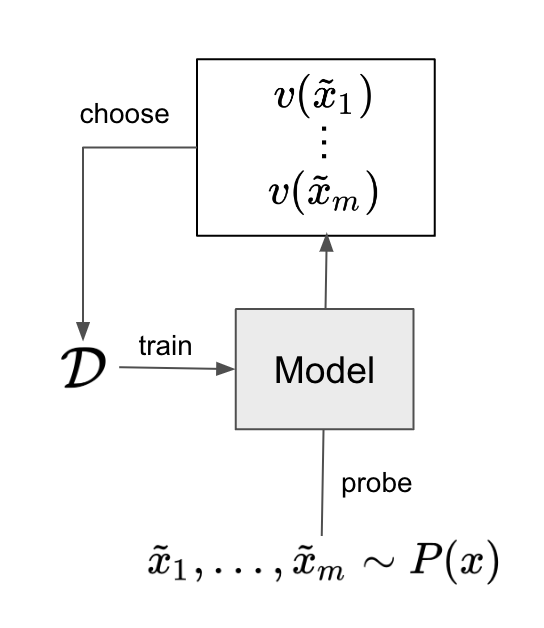
\includegraphics[width=0.4\textwidth,height=\textheight]{src/Figures/active_learning_schema.png}

}

\caption{\label{fig-schema}The current model is trained on the current
data set \(\mathcal{D}\). Potential points
\(\tilde{x}_1, \ldots, \tilde{x}_m\) are being investigated, and one of
them will be chosen and added to the data set. A proxy highlights the
relative value of each point in terms of improving the model, denoted by
\(v(\tilde{x}_1), \ldots, v(\tilde{x}_m)\). The point with the highest
value is selected and added to \(\mathcal{D}\). This cycle repeats until
enough data has been collected or the model is good enough.}

\end{figure}%

Within this decision process Figure~\ref{fig-schema}, the model is never
actually trained on those prospective points. The estimate of the added
value of a point can be correct, but it can also diverge from reality.
If the strategy used is effective, then the model not only improves, but
it could also do so using much less data than if it was trained on a
dataset built manually without exploiting the model feedback.

Active learning has been successfully applied to various domains to
enhance real-world systems, including computer vision, natural language
processing, and recommender systems. For example, active learning may be
used to improve the computer vision models used in autonomous vehicles
(\citeproc{ref-AL_app_autonomous}{Jarl et al. 2021}), where driving
scenes can take infinitely many forms and gathering an exhaustive data
set is impossible. Instead, probing a model and understanding what type
of data it would benefit from sounds more practical. In robotics,
autonomous agents may query humans when unsure how to act or face new
situations (\citeproc{ref-AL_app_robotics}{Taylor, Berrueta, and Murphey
2021}). In this space, there is often a significant financial and time
cost incurred for collecting data: the robot must act in real-time in
the real world, and while parallelization is possible, being strategic
about which examples should be collected to best benefit the model
helps. In meteorology, active learning can help decide where to place
additional sensors for weather predictions
(\citeproc{ref-AL_app_sensors}{Singh, Nowak, and Ramanathan 2006}).
Sensor placement involves deploying teams of people to remote locations
and expensive construction for an extra data point. Choosing these
locations and where to allocate resources wisely interests governments
and businesses. Active learning could also be employed to select data
for fine-tuning LLMs for specific downstream tasks
(\citeproc{ref-AL_app_LLMs}{Margatina et al. 2023}). In this space, it
might be difficult to fully describe an NLP task one might want an LLM
to solve. Often, instead of defining a task via a dataset of examples,
it may be easier for the human to interact with the LLM for a specific
use case, find holes in the model, and cover those using active
learning.

\subsection{Introduction to Active Preference
Learning}\label{introduction-to-active-preference-learning}

Consider the scenario where a robot is being trained to assist
individuals with feeding. How can such a robot be effectively taught to
perform necessary tasks, such as determining the appropriate distance to
reach, detecting the location of a person's mouth, and, most
importantly, understanding human preferences? In most cases, robots
learn by observing human demonstrations, where they replicate the ways a
person performs the task. However, this method poses significant
challenges. Expert demonstrations are often limited, and training a
supervised learning model would require vast amounts of demonstration
data, which is difficult to obtain at scale. Moreover, demonstrations
tend to be variable, as they reflect the actions of individual humans,
making the data collection process inconsistent. To address these
limitations, alternative approaches have been proposed, such as using
pairwise comparisons, where humans evaluate two action trajectories to
determine the superior one, or employing physical corrections, in which
reward functions are learned through human-robot interactions, with
humans guiding the robot's actions during the task.

Active learning algorithms can be employed in preference learning tasks,
such as the previously mentioned example, where the objective is to
develop a model that aligns with human preferences while minimizing the
need for extensive labeled data or reducing the high cost of
annotations. This chapter will explore the theoretical foundations of
pairwise comparisons and active preference learning, along with
extensions to these methods that address known limitations. Practical
examples where these approaches prove beneficial will also be discussed.
Additionally, we will examine the role of Large Language Models (LLMs)
in assisting robots through corrective feedback and highlight the
applications of these techniques.

\subsection{Uncertainty Qualification}\label{uncertainty-qualification}

\textbf{Problem Setup}: In this section, we will consider a binary
classification problem. The model is trained on a small labeled dataset
\(\mathcal{D} = \{(x_1, y_1), \ldots, (x_n, y_n)\}\), where \(x_i\)
represents the input data and \(y_i\) is the corresponding label. The
model is uncertain about the class labels of some data points and can
query an oracle to obtain the true labels of these data points. The goal
is to minimize the number of queries to the oracle while maximizing the
model's performance.

Uncertainty quantification (UQ) is a critical aspect of active learning
that allows models to evaluate the informativeness of new data points.
In machine learning (ML), two primary types of uncertainty are often
considered: epistemic and aleatoric uncertainty. \textbf{Epistemic
uncertainty}, or model uncertainty, arises from a lack of knowledge and
can be reduced by acquiring more data. This type of uncertainty is
especially significant when the model lacks confidence due to
insufficient or incomplete information in its training set. On the other
hand, \textbf{aleatoric uncertainty}, or data uncertainty, stems from
the inherent randomness within the data itself. Unlike epistemic
uncertainty, aleatoric uncertainty cannot be reduced, even with
additional data, as it reflects noise or unpredictability in the real
data-generating process.

Several approaches exist to quantify uncertainty in active learning,
each with its strengths and limitations. \textbf{Bayesian methods}, such
as Bayesian Neural Networks (BNNs) and Gaussian Processes (GPs), offer a
principled way of estimating uncertainty by incorporating prior
knowledge into the model. These approaches can generate meaningful
uncertainty estimates that aid in choosing informative samples for
labeling. However, they can become computationally prohibitive,
especially for large and complex models, limiting their applicability in
some practical scenarios.

Another common technique for uncertainty quantification is the use of
\textbf{ensemble methods}, such as Random Forests or Gradient Boosting
Machines. These methods involve training multiple models and combining
their predictions to provide an estimate of uncertainty. Ensemble
methods are relatively easy to implement and can give valuable insights
into model uncertainty. However, they can be computationally expensive
and may not always produce well-calibrated uncertainty estimates.
Moreover, they do not integrate prior knowledge, which can be a
disadvantage in certain applications.

\textbf{Conformal prediction methods} also provide a framework for
estimating uncertainty by offering a measure of confidence in
predictions based on the conformity of a given instance with the
training data. While these methods are useful in some contexts, this
book focuses primarily on the Bayesian approach due to its theoretical
robustness and capacity to quantify uncertainty in a more comprehensive
manner.

\subsection{Acquisition Function}\label{acquisition-function}

Uncertainty quantification plays a vital role in \textbf{acquisition
functions}, which are central to active learning strategies. These
functions determine which samples are most valuable to label by
evaluating their utility based on the model's current uncertainty
estimates. Common acquisition functions include \textbf{uncertainty
sampling} (\citeproc{ref-AL_uncertainty}{Zhu et al. 2010}), which
selects samples the model is least confident about,
\textbf{query-by-committee} (\citeproc{ref-AL_committee}{Beluch et al.
2018}), which utilizes a set of models to choose the most uncertain
samples, and \textbf{Bayesian Active Learning by Disagreement (BALD)}
(\citeproc{ref-AL_BALD}{Houlsby et al. 2011}), which selects samples
that maximize information gain by reducing model uncertainty. Through
careful uncertainty quantification, acquisition functions guide the
active learning process, improving the model's efficiency in learning
from limited data. Other acquisition functions can also be employed
listed below:

\begin{itemize}
\item
  Active Thompson Sampling (\citeproc{ref-AL_exploreexploit}{Bouneffouf
  et al. 2014}): This method leverages the Thompson Sampling algorithm
  to select a posterior sample from the model's distribution and compute
  the expected utility of labeling using that sample. By doing so, the
  algorithm balances exploration and exploitation, leading to effective
  active learning.
\item
  Expected model change (\citeproc{ref-AL_expmodelchange}{Cai, Zhang,
  and Zhou 2013}): This approach focuses on labeling points that would
  have the most impact on changing the current model parameters.
\item
  Expected error reduction (\citeproc{ref-AL_experrorredn}{Mussmann et
  al. 2022}): Points that would most effectively reduce the model's
  generalization error are labeled using this strategy.
\item
  Variance reduction (\citeproc{ref-AL_variance}{Cohn, Ghahramani, and
  Jordan 1996}): This approach labels points that would minimize output
  variance, which is one component of error. By selecting points that
  reduce variability in the model's predictions, it aims to improve its
  overall performance.
\item
  User Centered Labeling Strategies
  (\citeproc{ref-AL_usercentered}{Bernard et al. 2018}): This approach
  involves actively involving the user in the labeling process by
  visualizing data through dimensionality reduction techniques. The user
  then provides labels for the compiled data based on their domain
  expertise and preferences. This strategy leverages user input to
  improve the quality and relevance of the labeled data.
\item
  Querying from diverse subspaces or partitions
  (\citeproc{ref-AL_partition}{Ma et al. 2022}): When using a forest of
  trees as the underlying model, the leaf nodes can represent
  overlapping partitions of the feature space. This strategy selects
  instances from non-overlapping or minimally overlapping partitions for
  labeling.
\item
  Conformal prediction (\citeproc{ref-AL_conformal}{Makili, Sánchez, and
  Dormido-Canto 2012}): This method predicts that a new data point will
  have a label similar to old data points in some specified way. The
  degree of similarity within the old examples is used to estimate the
  confidence in the prediction.
\item
  Mismatch-first farthest-traversal (\citeproc{ref-AL_mismatch}{Zhao,
  Heittola, and Virtanen 2020}): This strategy first prioritizes data
  points that are wrongly predicted by the current model compared to the
  nearest-neighbor prediction. The second criterion is the distance to
  previously selected data, with preference given to those that are
  farthest away. The goal is to optimize both the correction of
  mispredictions and the diversity of the selected data.
\end{itemize}

\subsubsection{Uncertainty Sampling}\label{uncertainty-sampling}

Uncertainty sampling (\citeproc{ref-AL_uncertainty}{Zhu et al. 2010}) is
a widely used acquisition function in active learning that selects data
points for which the model exhibits the greatest uncertainty. This
method aims to improve model performance by focusing labeling efforts on
ambiguous samples, where additional information is likely to yield the
greatest benefit. Let \(x\) represent the input, and \(p(y|x)\) the
probability distribution of the output \(y\) given \(x\). Several
acquisition strategies fall under uncertainty sampling, including
\textbf{entropy sampling}, \textbf{margin sampling}, and \textbf{least
confidence sampling}, each providing a unique measure of uncertainty.

\begin{itemize}
\item
  \textbf{Entropy sampling} measures the uncertainty by calculating the
  entropy of the predicted probability distribution. The acquisition
  function is given by \(\alpha(x) = - \sum_{y} p(y|x) \log p(y|x)\),
  with higher entropy values indicating higher uncertainty.
\item
  \textbf{Margin sampling} focuses on the difference between the two
  highest predicted probabilities for a sample. The acquisition function
  is given by \(\alpha(x) = p(y_1|x) - p(y_2|x)\), where \(y_1\) and
  \(y_2\) are the most likely classes. Smaller margins signify greater
  uncertainty.
\item
  \textbf{Least confidence sampling} measures uncertainty by identifying
  the sample with the lowest predicted probability for its most likely
  class. The acquisition function is
  \(\alpha(x) = 1 - p(y_{\text{max}}|x)\), where \(y_{\text{max}}\) is
  the class with the highest probability.
\end{itemize}

\textbf{Example:} Consider a binary classification problem with two
classes \(y_1\) and \(y_2\). We have three samples \(x_1, x_2, x_3\) and
the corresponding predictive distributions are as follows:
\[\begin{aligned}
p(y_1|x_1) &= 0.6, \quad p(y_2|x_1) = 0.4\\
p(y_1|x_2) &= 0.3, \quad p(y_2|x_2) = 0.7\\
p(y_1|x_3) &= 0.8, \quad p(y_2|x_3) = 0.2
\end{aligned}\]

\begin{itemize}
\tightlist
\item
  \textbf{Entropy Sampling}

  \begin{itemize}
  \tightlist
  \item
    \(\alpha(x_1) = -0.6 \log (0.6) - 0.4 \log (0.4) = 0.29\)
  \item
    \(\alpha(x_2) = -0.3 \log (0.3) - 0.7 \log (0.7) = 0.27\)
  \item
    \(\alpha(x_3) = -0.8 \log (0.8) - 0.2 \log (0.2) = 0.22\)
  \end{itemize}
\end{itemize}

We would select \(x_1\) for labeling as it has the highest entropy,
indicating the model is most uncertain about its prediction at \(x_1\).

\begin{itemize}
\tightlist
\item
  \textbf{Margin Sampling}

  \begin{itemize}
  \tightlist
  \item
    \(\alpha(x_1) = 0.6 - 0.4 = 0.2\)
  \item
    \(\alpha(x_2) = 0.7 - 0.3 = 0.4\)
  \item
    \(\alpha(x_3) = 0.8 - 0.2 = 0.6\)
  \end{itemize}
\end{itemize}

We would select \(x_1\) for labeling as it has the smallest margin,
indicating the model is most uncertain about the prediction at \(x_1\).

\begin{itemize}
\tightlist
\item
  \textbf{Least Confidence Sampling}

  \begin{itemize}
  \tightlist
  \item
    \(\alpha(x_1) = 1 - 0.6 = 0.4\)
  \item
    \(\alpha(x_2) = 1 - 0.7 = 0.3\)
  \item
    \(\alpha(x_3) = 1 - 0.8 = 0.2\)
  \end{itemize}
\end{itemize}

We would select \(x_1\) for labeling as it has the lowest confidence,
indicating the model is most uncertain about the prediction at \(x_1\).

In summary, uncertainty sampling methods, whether based on entropy,
margin, or least confidence, help prioritize data points that the model
struggles with the most. By focusing on these uncertain samples, the
model can more efficiently improve its performance, making uncertainty
sampling a key tool in active learning.

\subsubsection{Query-by-Committee}\label{query-by-committee}

Query-by-Committee (\citeproc{ref-AL_committee}{Beluch et al. 2018}) is
an active learning strategy where a committee of models selects samples
for labeling based on the level of disagreement among the committee
members. Several acquisition functions can be employed under this
framework to quantify the disagreement:

\begin{itemize}
\tightlist
\item
  \textbf{Vote Entropy:} The vote entropy measures the uncertainty based
  on how often the committee members vote for each class. The
  acquisition function is defined as
  \(\alpha(x) = \mathbb{H}\left[\frac{V(y)}{C}\right]\), where \(V(y)\)
  is the number of votes for class \(y\) and \(C\) is the number of
  committee members.
\item
  \textbf{Consensus Entropy:} This acquisition function measures the
  entropy of the average probability distribution across committee
  members. It is given by \(\alpha(x) = \mathbb{H}[P_C(y|x)]\), where
  \(P_C(y|x)\) is the average probability distribution for sample \(x\)
  across all committee members.
\item
  \textbf{KL Divergence:} The KL divergence quantifies the disagreement
  by comparing the probability distribution of each committee member to
  the average distribution. The acquisition function is given by
  \(\alpha(x) = \frac{1}{C} \sum_{c=1}^{C} D_{KL}[P_c(y|x) || P_C(y|x)]\),
  where \(P_c(y|x)\) is the probability distribution of committee member
  \(c\) and \(P_C(y|x)\) is the average distribution across the
  committee.
\end{itemize}

\textbf{Example:} Consider a binary classification problem with two
classes \(y_1\) and \(y_2\). We have three committee members and three
samples: \(x_1\), \(x_2\), and \(x_3\). The predictive distributions for
each committee member are given below:

\begin{longtable}[]{@{}
  >{\raggedright\arraybackslash}p{(\columnwidth - 12\tabcolsep) * \real{0.0382}}
  >{\raggedright\arraybackslash}p{(\columnwidth - 12\tabcolsep) * \real{0.1603}}
  >{\raggedright\arraybackslash}p{(\columnwidth - 12\tabcolsep) * \real{0.1603}}
  >{\raggedright\arraybackslash}p{(\columnwidth - 12\tabcolsep) * \real{0.1603}}
  >{\raggedright\arraybackslash}p{(\columnwidth - 12\tabcolsep) * \real{0.1603}}
  >{\raggedright\arraybackslash}p{(\columnwidth - 12\tabcolsep) * \real{0.1603}}
  >{\raggedright\arraybackslash}p{(\columnwidth - 12\tabcolsep) * \real{0.1603}}@{}}
\toprule\noalign{}
\begin{minipage}[b]{\linewidth}\raggedright
\(x\)
\end{minipage} & \begin{minipage}[b]{\linewidth}\raggedright
\(p_1(y_1 \vert \cdot)\)
\end{minipage} & \begin{minipage}[b]{\linewidth}\raggedright
\(p_1(y_2 \vert \cdot)\)
\end{minipage} & \begin{minipage}[b]{\linewidth}\raggedright
\(p_2(y_1 \vert \cdot)\)
\end{minipage} & \begin{minipage}[b]{\linewidth}\raggedright
\(p_2(y_2 \vert \cdot)\)
\end{minipage} & \begin{minipage}[b]{\linewidth}\raggedright
\(p_3(y_1 \vert \cdot)\)
\end{minipage} & \begin{minipage}[b]{\linewidth}\raggedright
\(p_3(y_2 \vert \cdot)\)
\end{minipage} \\
\midrule\noalign{}
\endhead
\bottomrule\noalign{}
\endlastfoot
\(x_1\) & 0.6 & 0.4 & 0.7 & 0.3 & 0.3 & 0.7 \\
\(x_2\) & 0.3 & 0.7 & 0.4 & 0.6 & 0.4 & 0.6 \\
\(x_3\) & 0.8 & 0.2 & 0.9 & 0.1 & 0.7 & 0.3 \\
\end{longtable}

\textbf{Query-by-Committee: Vote Entropy}

\begin{itemize}
\tightlist
\item
  For sample \(x_1\), the votes for \(y_1\) and \(y_2\) are
  \(V(y_1) = 2\) and \(V(y_2) = 1\). The vote entropy is
  \(\alpha(x_1) = - \frac{2}{3} \log (\frac{2}{3}) - \frac{1}{3} \log (\frac{1}{3}) = 0.28\).
\item
  For sample \(x_2\), the votes are \(V(y_1) = 0\) and \(V(y_2) = 3\),
  resulting in vote entropy \(\alpha(x_2) = 0\).
\item
  For sample \(x_3\), the votes are \(V(y_1) = 3\) and \(V(y_2) = 0\),
  resulting in vote entropy \(\alpha(x_3) = 0\).
\end{itemize}

Thus, sample \(x_1\) would be selected for labeling as it has the
highest vote entropy, indicating the greatest disagreement among the
committee members.

\textbf{Query-by-Committee: Consensus Entropy}

The first step is to compute the consensus probability of each class for
each sample:

\begin{itemize}
\tightlist
\item
  For \(x_1\), \(p_c(y_1|x_1) = \frac{0.6 + 0.7 + 0.3}{3} = 0.53\) and
  \(p_c(y_2|x_1) = \frac{0.4 + 0.3 + 0.7}{3} = 0.47\).
\item
  For \(x_2\), \(p_c(y_1|x_2) = \frac{0.3 + 0.4 + 0.4}{3} = 0.37\) and
  \(p_c(y_2|x_2) = \frac{0.7 + 0.6 + 0.6}{3} = 0.63\).
\item
  For \(x_3\), \(p_c(y_1|x_3) = \frac{0.8 + 0.9 + 0.7}{3} = 0.8\) and
  \(p_c(y_2|x_3) = \frac{0.2 + 0.1 + 0.3}{3} = 0.2\).
\end{itemize}

Next, we compute the entropy of these consensus probabilities:

\begin{itemize}
\tightlist
\item
  For \(x_1\),
  \(\mathbb{H}[p_c(y|x_1)] = -0.53 \log (0.53) - 0.47 \log (0.47) = 0.30\).
\item
  For \(x_2\),
  \(\mathbb{H}[p_c(y|x_2)] = -0.37 \log (0.37) - 0.63 \log (0.63) = 0.29\).
\item
  For \(x_3\),
  \(\mathbb{H}[p_c(y|x_3)] = -0.8 \log (0.8) - 0.2 \log (0.2) = 0.22\).
\end{itemize}

Thus, \(x_1\) would be selected for labeling as it has the highest
consensus entropy, indicating the highest level of disagreement among
the committee members.

\subsubsection{Bayesian Active Learning by
Disagreement}\label{bayesian-active-learning-by-disagreement}

Bayesian Active Learning by Disagreement (BALD)
(\citeproc{ref-AL_BALD}{Houlsby et al. 2011}) selects the samples for
which the model expects to gain the most Shannon information when
corresponding labels are observed:

\[
\mathbb{I}(\theta; y|x, \mathcal{D}) = \mathbb{H}[p(y|x, \mathcal{D})] - \mathbb{E}_{p(\theta | \mathcal{D})} [\mathbb{H}[p(y|x, \theta, \mathcal{D})]]
\]

where \(\mathbb{H}[\cdot]\) denotes entropy. When there is significant
disagreement among models, the predictive entropy (the first term) will
be large, while the expected entropy (the second term) will be smaller.
This difference represents the degree to which the models disagree. BALD
selects points where this disagreement is maximized.

\begin{itemize}
\tightlist
\item
  To compute the first term, we can derive the following expression:
\end{itemize}

\[
\mathbb{H}[p(y|x, \mathcal{D})] = \mathbb{H}\left[\int_{\theta} p(y|x, \theta, \mathcal{D}) p(\theta | \mathcal{D}) d\theta\right] \approx \mathbb{H}\left[\frac{1}{N}\sum_{i=1}^{N} p(y|x, \theta_i, \mathcal{D})\right] = \mathbb{H}\left[\overline{p}(y|x, \mathcal{D})\right]
\]

\begin{itemize}
\tightlist
\item
  To compute the second term, we can derive the following expression:
\end{itemize}

\[\begin{aligned}
\mathbb{E}_{p(\theta|\mathcal{D})} [\mathbb{H}[p(y|x, \theta, \mathcal{D})]] &= \mathbb{E}_{p(\theta|\mathcal{D})} \left[ - \sum_{y} p(y|x, \theta, \mathcal{D}) \log p(y|x, \theta, \mathcal{D}) \right] \\
&\approx - \frac{1}{N} \sum_{i=1}^{N} \left( \sum_{y} p(y|x, \theta_i, \mathcal{D}) \log p(y|x, \theta_i, \mathcal{D}) \right)
\end{aligned}\]

\textbf{Example:} Consider a binary classification problem with two
classes, \(y_1\) and \(y_2\). We have two samples, \(x_1\) and \(x_2\),
and the model's predictive distributions are as follows:

\begin{itemize}
\item
  \textbf{First-time inference} (with
  \(\theta_1 \sim p(\theta | \mathcal{D})\)): \[
  p(y_1|x_1, \theta_1, \mathcal{D}) = 0.6, \quad p(y_2|x_1, \theta_1, \mathcal{D}) = 0.4
  \] \[
  p(y_1|x_2, \theta_1, \mathcal{D}) = 0.4, \quad p(y_2|x_2, \theta_1, \mathcal{D}) = 0.6
  \]
\item
  \textbf{Second-time inference} (with
  \(\theta_2 \sim p(\theta | \mathcal{D})\)): \[
  p(y_1|x_1, \theta_2, \mathcal{D}) = 0.8, \quad p(y_2|x_1, \theta_2, \mathcal{D}) = 0.2
  \] \[
  p(y_1|x_2, \theta_2, \mathcal{D}) = 0.5, \quad p(y_2|x_2, \theta_2, \mathcal{D}) = 0.5
  \]
\end{itemize}

\textbf{Solution:}

\textbf{Step 1:} Compute the entropy of the model's predictive
distribution for each sample:

\begin{itemize}
\tightlist
\item
  \(\overline{p}_{\theta}(y_1|x_1, \theta, \mathcal{D}) = 0.7\)
\item
  \(\overline{p}_{\theta}(y_2|x_1, \theta, \mathcal{D}) = 0.3\)
\item
  \(\overline{p}_{\theta}(y_1|x_2, \theta, \mathcal{D}) = 0.45\)
\item
  \(\overline{p}_{\theta}(y_2|x_2, \theta, \mathcal{D}) = 0.55\)
\end{itemize}

Now, we compute the entropy for each sample using the formula:

\[
\mathbb{H}[p(y|x, \mathcal{D})] = - p(y_1|x, \mathcal{D}) \log(p(y_1|x, \mathcal{D})) - p(y_2|x, \mathcal{D}) \log(p(y_2|x, \mathcal{D}))
\]

For \(x_1\):

\[
\mathbb{H}[p(y|x_1, \mathcal{D})] = - 0.7 \log(0.7) - 0.3 \log(0.3) = 0.27
\]

For \(x_2\):

\[
\mathbb{H}[p(y|x_2, \mathcal{D})] = - 0.45 \log(0.45) - 0.55 \log(0.55) = 0.30
\]

\textbf{Step 2:} Compute the expected entropy of the model's predictive
distribution for each sample.

For \(x_1\):

\begin{itemize}
\tightlist
\item
  \(\mathbb{H}_{\theta_1}[p(y|x_1, \theta, \mathcal{D})] = -0.6 \log(0.6) - 0.4 \log(0.4) = 0.29\)
\item
  \(\mathbb{H}_{\theta_2}[p(y|x_1, \theta, \mathcal{D})] = -0.8 \log(0.8) - 0.2 \log(0.2) = 0.22\)
\end{itemize}

Average the results:

\[
\mathbb{E}_{p(\theta|\mathcal{D})}[\mathbb{H}[p(y|x_1, \theta, \mathcal{D})]] \approx \frac{0.29 + 0.22}{2} = 0.255
\]

For \(x_2\):

\begin{itemize}
\tightlist
\item
  \(\mathbb{H}_{\theta_1}[p(y|x_2, \theta, \mathcal{D})] = -0.4 \log(0.4) - 0.6 \log(0.6) = 0.29\)
\item
  \(\mathbb{H}_{\theta_2}[p(y|x_2, \theta, \mathcal{D})] = -0.5 \log(0.5) - 0.5 \log(0.5) = 0.30\)
\end{itemize}

Average the results:

\[
\mathbb{E}_{p(\theta|\mathcal{D})}[\mathbb{H}[p(y|x_2, \theta, \mathcal{D})]] \approx \frac{0.29 + 0.30}{2} = 0.295
\]

\textbf{Step 3:} Compute the BALD score for each sample.

The BALD score \(\alpha(x)\) is the difference between the predictive
entropy and the expected entropy:

For \(x_1\):

\[
\alpha(x_1) = \mathbb{H}[p(y|x_1, \mathcal{D})] - \mathbb{E}_{p(\theta|\mathcal{D})}[\mathbb{H}[p(y|x_1, \theta, \mathcal{D})]] = 0.27 - 0.255 = 0.015
\]

For \(x_2\):

\[
\alpha(x_2) = \mathbb{H}[p(y|x_2, \mathcal{D})] - \mathbb{E}_{p(\theta|\mathcal{D})}[\mathbb{H}[p(y|x_2, \theta, \mathcal{D})]] = 0.30 - 0.295 = 0.005
\]

We would select \(x_1\) for labeling since it has the highest BALD
score, indicating that labeling \(x_1\) will provide the most
information gain for the model.

\subsection{Active Learning by Variance
Reduction}\label{active-learning-by-variance-reduction}

Active Learning by Variance Reduction (\citeproc{ref-AL_variance}{Cohn,
Ghahramani, and Jordan 1996}) is an algorithm that selects the next data
point to label based on the expected reduction in the model's variance.
The goal is to choose the point \(\tilde{x} \sim p(x)\) that, when
labeled (\(y(\tilde{x})\)), will reduce the model's variance the most.
To quantify the expected error at a given input \(x\), we can
mathematically express it as follows:

\[
\mathbb{E}_{\hat{y} \sim p(\hat{y} | \mathcal{D}; x), y \sim p(y|x)} (\hat{y} - y)^2
\]

In this expression, \(\hat{y}\) represents the model's prediction, while
\(y\) denotes the true label corresponding to the input \(x\). This
formulation captures the average squared difference between the
predicted and actual values, providing a measure of the model's
accuracy. Utilizing concepts from bias-variance decomposition as
outlined in the literature
(\citeproc{ref-bias_variance_orig_paper}{Geman, Bienenstock, and Doursat
1992}), we can expand the expected error term. The expansion is given
by:

\[\begin{aligned}
\mathbb{E}_{\hat{y} \sim p(\hat{y} | \mathcal{D}; x), y \sim p(y|x)} (\hat{y} - y)^2 &= \mathbb{E}_{\hat{y}, y}[(\hat{y} - \mathbb{E}[y|x]) + (\mathbb{E}[y|x] - y)]^2 \\
&= \mathbb{E}_{\hat{y}, y} [(y - \mathbb{E}[y|x])^2] + 2\mathbb{E}_{\hat{y}, y} [(\hat{y} - \mathbb{E}[y|x])(\mathbb{E}[y|x] - y)] + \mathbb{E}_{\hat{y}, y}(\hat{y} - \mathbb{E}[y|x])^2
\end{aligned}\]

In this equation, the first term represents the variance of the true
label \(y\), the second term evaluates to zero, and the third term
accounts for the variance of the model's prediction \(\hat{y}\). To
clarify why the second term is zero, we note that:

\[
\mathbb{E}_{\hat{y}, y}[\mathbb{E}[y|x] - y] = 0
\]

This indicates that the expected deviation of the true label from its
conditional mean is null, as \(\mathbb{E}[y|x]\) is, by definition, the
average of \(y\) given \(x\). Focusing on the third term, we derive it
as follows:

\[\begin{aligned}
\mathbb{E}_{\hat{y}, y}(\hat{y} - \mathbb{E}[y|x])^2 &= \mathbb{E}_{\hat{y}, y}[(\hat{y} - \mathbb{E}_{\hat{y}}[\hat{y}] + \mathbb{E}_{\hat{y}}[\hat{y}] - \mathbb{E}[y|x])^2] \\
&= \mathbb{E}_{\hat{y}, y}[(\hat{y} - \mathbb{E}_{\hat{y}}[\hat{y}])^2] + (\mathbb{E}_{\hat{y}}[\hat{y}] - \mathbb{E}[y|x])^2
\end{aligned}\]

Here, \(\mathbb{E}_{\hat{y}}[\hat{y}]\) represents the expected model
prediction conditioned on the data \(\mathcal{D}\) and input \(x\).
Combining the results of our analysis, we arrive at the total expected
error as:

\[
\mathbb{E}_{y} [(y - \mathbb{E}[y|x])^2] + (\mathbb{E}_{\hat{y}} [\hat{y} - \mathbb{E}[y|x]] )^2 + \mathbb{E}_{\hat{y}} [(\hat{y} - \mathbb{E}_{\hat{y}}[\hat{y}])^2]
\]

In this equation, the first term signifies the variance of the true
label, which remains constant for a given \(x\). The second term
captures the bias of the model, reflecting how much the average model
prediction deviates from the expected true label. The third term
quantifies the model's uncertainty concerning the selected input \(x\).

Referring to (\citeproc{ref-AL_variance}{Cohn, Ghahramani, and Jordan
1996}), we can denote the uncertainty term as:

\[
\sigma^2_{\hat{y}} (x | \mathcal{D}) = \mathbb{E}_{\hat{y}} [(\hat{y} - \mathbb{E}_{\hat{y}}[\hat{y}])^2]
\]

This term explicitly represents the variance of the model predictions at
the input \(x\) given the dataset \(\mathcal{D}\). More explicitly, it
can be expressed as:

\[
\sigma^2_{\hat{y}} (x | \mathcal{D}) =  \mathbb{E}_{\hat{y} \sim p(\hat{y} | \mathcal{D}; x)} [(\hat{y} - \mathbb{E}_{\hat{y} \sim p(\hat{y} | \mathcal{D}; x)}[\hat{y}])^2]
\]

This formulation emphasizes the variability of the model's predictions
around their mean, providing insights into the model's reliability in
its estimations.

\textbf{Algorithm:} The active learning by variance reduction algorithm
can be summarized as follows:

\begin{enumerate}
\def\labelenumi{\arabic{enumi}.}
\tightlist
\item
  \textbf{Sampling Candidates}: Sample candidate points
  \(\tilde{x}_1, \dots, \tilde{x}_m\) from \(p(x)\).
\item
  \textbf{Compute Expected Variance Reduction}: For each candidate
  \(\tilde{x}_i\), compute: \[
  \mathbb{E}_{p(x)} [\sigma^2_{\hat{y}} (x | \tilde{\mathcal{D}})]
  \]
\item
  \textbf{Select the Best Candidate}: Choose the point that minimizes
  expected variance reduction: \[
     \tilde{x}^* = \arg\min_{\tilde{x}_i} \mathbb{E}_{p(x)} [\sigma^2_{\hat{y}} (x | \tilde{\mathcal{D}})]
  \]
\item
  \textbf{Update Model}: Incorporate the newly labeled data and repeat
  the process.
\end{enumerate}

While there is no general recipe for the number of iterations to
perform, one could imagine relying on some empirical measure like a loss
on left-out labelled data to gauge model improvement (as seen in
Figure~\ref{fig-empirical:gauss}, Figure~\ref{fig-empirical:regress}).
Intuitively, the size of the data set and its relationship to the loss
is intimately tied to the model complexity which impacts its
data-thirstiness.

We note to the reader that \(P(X=x)\) is a distribution with
potentially-infinite support and the authors do not compute this
integral exactly. Instead, the computational estimate of that integral
consists of sampling several points \(x \sim P(X=x)\) and averaging the
quantity inside the integral over these points until convergence using
Monte-Carlo sampling approaches (see (\citeproc{ref-monte-carlo}{Ghojogh
et al. 2020})).

We note that the paper derives closed-form solutions to the expected
learner variance (\textbf{?@eq-ELV\_at\_x}) for two models
(Figure~\ref{fig-two_models}): (1) a mixture of Gaussian model and (2) a
locally-weighted regression model (Figure~\ref{fig-two_models}). We
refer the reader to the paper for the mathematical derivation of those
quantities.

\begin{figure}

\centering{

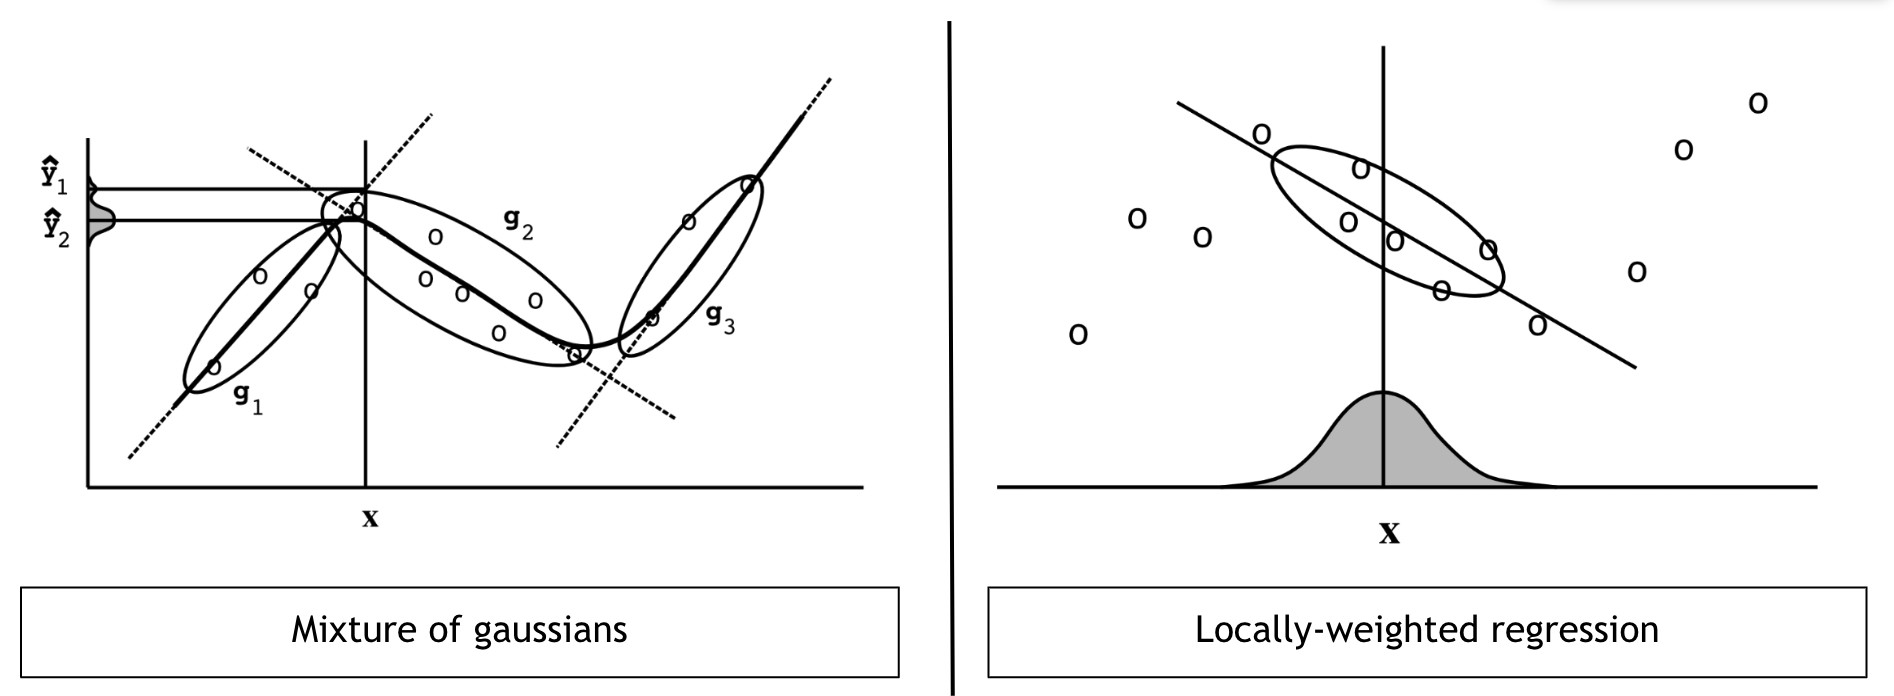
\includegraphics[width=1\textwidth,height=\textheight]{src/Figures/1_two_models.png}

}

\caption{\label{fig-two_models}Two models were empirically explored.
These two models lead to closed-form, accurately and
efficiently-computed expected learner variance which can be plugged into
the algorithm.}

\end{figure}%

Arm2D (Figure~\ref{fig-arm2D}) is a kinematics problem where learner has
to predict the tip position of a robotic arm given a set of joint angles
\(\mathbf{\theta_1}, \mathbf{\theta_2}\). In this analysis, the two
models seen in Figure~\ref{fig-two_models}, namely the Gaussian mixture
model and locally-weighted regression.

\begin{figure}

\centering{

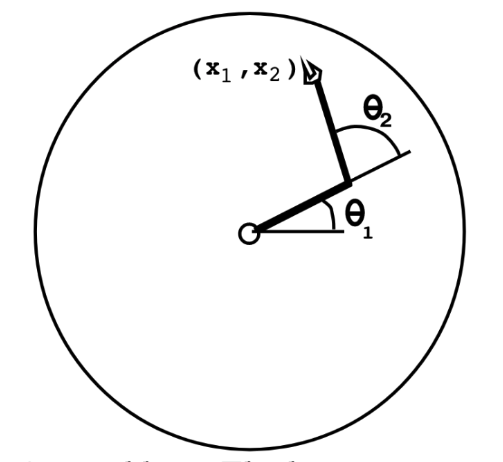
\includegraphics[width=0.4\textwidth,height=\textheight]{src/Figures/1_experiment_setup.png}

}

\caption{\label{fig-arm2D}The arm kinematics problem. The learner
attempts to predict tip position given a set of joint angles
\(\mathbf{\theta_1}, \mathbf{\theta_2}\)}

\end{figure}%

\begin{figure}

\centering{

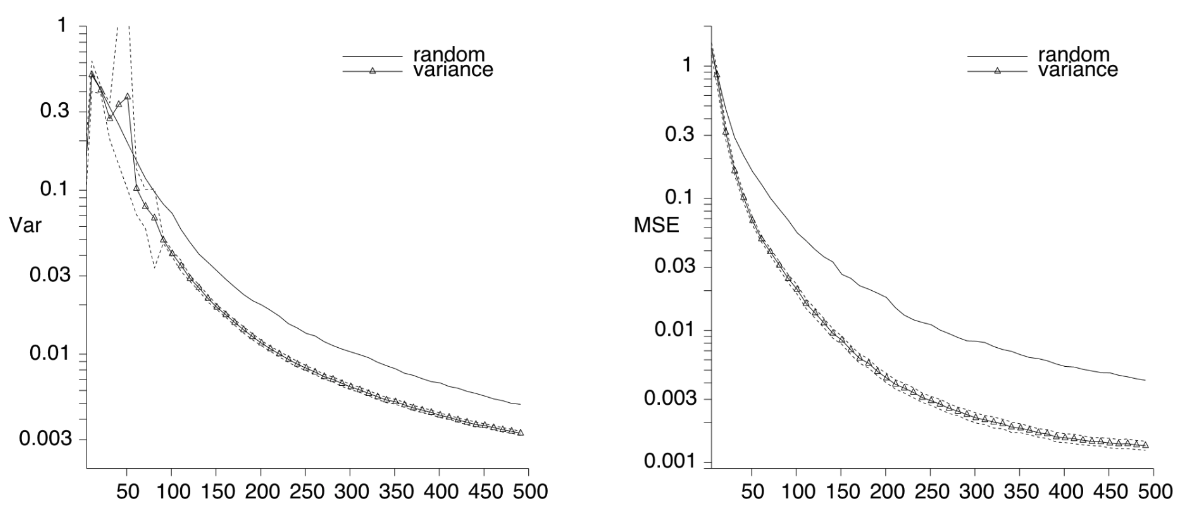
\includegraphics[width=1\textwidth,height=\textheight]{src/Figures/1_experiment_results_gaussian.png}

}

\caption{\label{fig-empirical:gauss}Arm2D domain. Dotted lines denote
standard error for average of 10 runs, each started with one initial
random example.}

\end{figure}%

What is interesting in the results seen
(Figure~\ref{fig-empirical:gauss}, Figure~\ref{fig-empirical:regress})
is that beyond the variance of the learner decreasing, as we would
expect, given that authors chose points to reduce the expected variance,
we do also see a related decrease in mean square error (MSE) of the
models, as the size of the collected data set increases, for \emph{both}
models. This is a cool result because the expected learner variance for
these models can be computed, relative to a new point, accurately and
efficiently, and we see that when plugged into the general active
learning loop (Figure~\ref{fig-schema}), model performance is enhanced
significantly.

What is surprising in the case of the locally-weighted regression model
(Figure~\ref{fig-empirical:regress}) is that if points were to be chosen
randomly, the MSE would be extremely unstable and have sharp increases
and decreases. But when the active learning by variance reduction is
used, with the expected learner variance as proxy, the MSE decreases
almost smoothly bar some preliminary instabilities.

\begin{figure}

\centering{

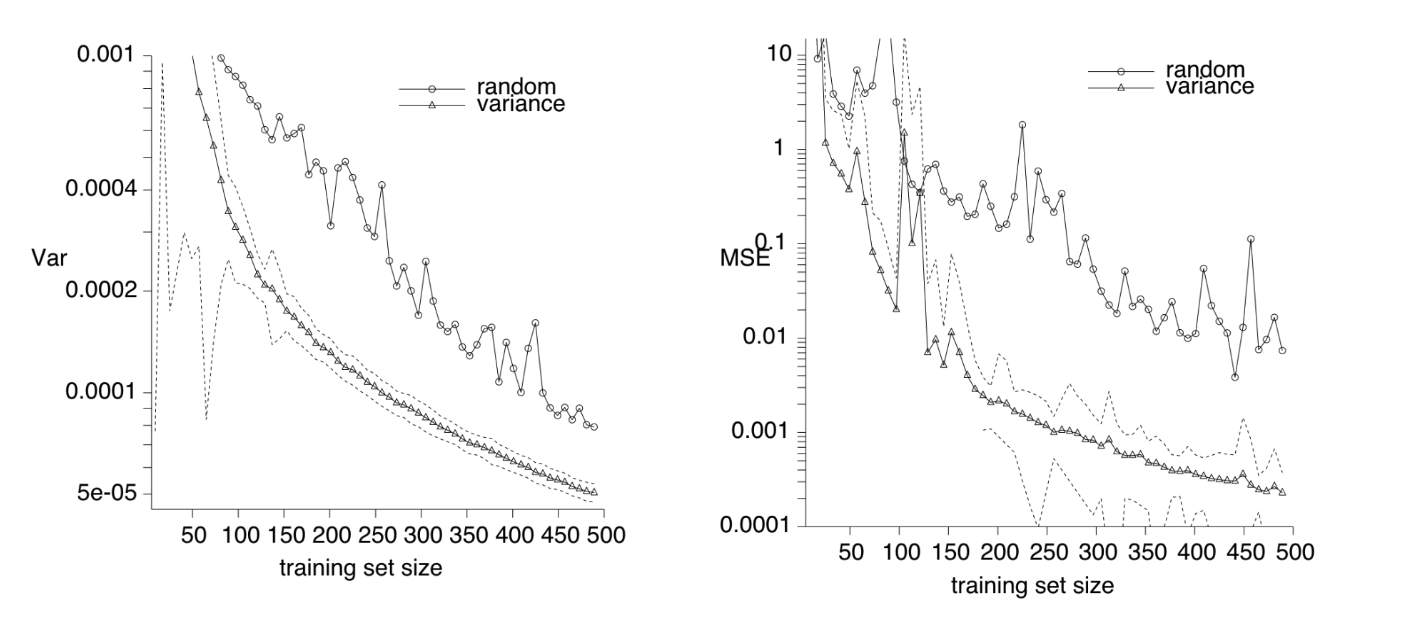
\includegraphics[width=1\textwidth,height=\textheight]{src/Figures/1_experiment_results_regression.png}

}

\caption{\label{fig-empirical:regress}Variance and MSE learning curves
for LOESS model trained on the Arm2D domain. Dotted lines denote
standard error for average of 60 runs, each started with a single
initial random example.}

\end{figure}%

\subsection{Active Learning in Ranking and
Comparison}\label{active-learning-in-ranking-and-comparison}

Many researchers have shown that making comparisons is an easier and
more convenient method for users than assigning a specific score for
each of the items demonstrated. Individual comparisons give out a full
ranking over a set of \(n\) objects
\(\Theta = (\theta_1, \theta_2, ..., \theta_n\)). That ranking will be
defined as a mapping \(\sigma : \{1,...,n\} \rightarrow \{1,...,n\}\)
that prescribes an order to the set of objects \(\Theta\). More
specifically, for a single \(\sigma\),
\(\sigma(\Theta) = \theta_{\sigma(1)} < \theta_{\sigma(2)} < ... < \theta_{\sigma(n-1)} < \theta_{\sigma(n)}\),
where \(\theta_{i} < \theta_{j}\) means that \(\theta_{i}\) is worse in
rating compared to \(\theta_{j}\).

For any \(n\) elements that there are to rank, there are \(n!\) possible
orderings over these elements that can result in the correct complete
ranking. Using the fact that a lower bound on sorting is \(n\log n\), to
get a guaranteed true rating over \(n\) objects one will need
\(n\log n\) pairwise comparisons if those comparisons are picked at
random. That number can be quite high and costly in many applications,
especially since most of the ranking information comes from humans, so
the more comparisons they have to make, the more money and time is
spent. This also might be inefficient since some comparisons can provide
more value to the learning process than others, meaning that some
comparisons are a waste to the process of deriving the ranking. This can
be detrimental in psychology and market research, as those fields
utilize comparisons the most, and a faster process might give a lot of
benefits.

The reason the lower bound on the number of comparisons is \(n\log n\)
is that it does not assume any information about the underlying space
and field, so the comparisons are chosen at random. However, if one is
to take advantage of the structures that are in the comparison space, it
might lead to more information about which comparisons will be most
valuable to ask for. For example, if abstracting to humans for a moment,
(\citeproc{ref-geo_paper}{G. and Nowak 2011}) discusses how eye doctors
have a big range of options to choose from when assigning prescriptions
for glasses, however, patients don't see them doing that many
comparisons before they decide which is the best option for a specific
client. That is because eye doctors have domain knowledge about the
field which they incorporate into the process, and only ask clients
questions for comparisons when needed. That gives rise to using similar
knowledge in the ranking field, which results in an active learning
approach that selects data based on the relevance of a comparison query
toward finding the final \(\sigma(\Theta)\).

\subsubsection{Geometric Approach to
Comparisons}\label{geometric-approach-to-comparisons}

In this part, we will go over a paper (\citeproc{ref-geo_paper}{G. and
Nowak 2011}), which dives deep into active learning over the data that
can be embedded into a multi-dimensional space. In that case, the
comparison that is done between two different objects splits the space
into halves, where in each half one object is better than the other. By
utilizing such spatial information, the paper creates a geometric
approach to ranking and active learning, and this spatial information
will be the domain knowledge that will help to determine which
comparisons to perform to get the ranking.

For this application, the following terms are defined:

\begin{enumerate}
\def\labelenumi{\arabic{enumi}.}
\item
  \(R^d\) is the space in which objects can be embedded
\item
  \(\theta_1,...,\theta_n\) the objects, and now will represent the
  locations of those objects in \(R^d\)
\item
  For each ranking \(\sigma\) there is a reference point
  \(r_{\sigma} \in R^d\), such that if according to ranking \(\sigma\),
  \(\theta_{i} < \theta_{j}\) (object \(i\) is worse than \(j\)), then
  \(||\theta_i - r_{\sigma}|| < ||\theta_j - r_{\sigma}||\), or
  otherwise object \(i\) is closer to the reference point \(r_\theta\)
  of the ranking than object \(j\).
\item
  \(\Sigma_{n,d}\) will be the set of all possible rankings of the \(n\)
  objects that satisfy the embedding distances in the space \(R^d\)
  defined in the previous term. Note that not all possible rankings will
  satisfy the embedding conditions, but on the other side, there might
  be multiple rankings that can satisfy all of those conditions too.
\item
  For every ranking \(\sigma\) there is \(M_n(\sigma)\) as the number of
  pairwise comparisons needed to identify the ranking. When comparisons
  are done at random \(E[M_n(\sigma)] = n\log n\), so the paper
  (\citeproc{ref-geo_paper}{G. and Nowak 2011}) will reason about this
  quantity to show that it can be smaller if incorporating the space
  knowledge.
\item
  \(q_{i,j}\) will be the query of comparison between objects \(i\) and
  \(j\).
\end{enumerate}

\subsubsection{Embedding Space}\label{embedding-space}

\begin{figure}

\centering{

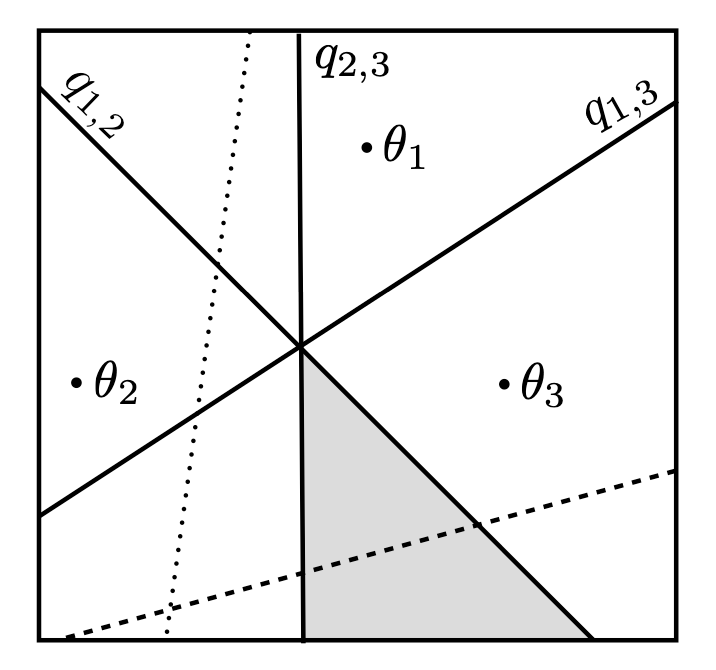
\includegraphics[width=0.4\textwidth,height=\textheight]{src/Figures/SPACE.png}

}

\caption{\label{fig-dim-space}Objects \(\theta_1, \theta_2, \theta_3\)
and queries in \(R^2\). The \(r_\theta\) lies in the shaded region which
represents \(\Sigma_{n,2}\)(consistent with the labels of
\(q_{1,2}, q_{1,3}, q_{2,3}\)). The dotted (dashed) lines represent new
queries whose labels are (are not) ambiguous.}

\end{figure}%

Next, we will discuss embedding space. To properly understand how to
select the most valuable queries, it is essential to discuss the space
where the objects exist and how the queries divide that space to find
the proper rankings. For this example, in Figure~\ref{fig-dim-space},
the paper (\citeproc{ref-geo_paper}{G. and Nowak 2011}) works in \(R^2\)
space, with three objects \(\theta_1\), \(\theta_2\), and \(\theta_3\).
There are pairwise queries \(q_{1,3}\), \(q_{2,3}\), \(q_{1,2}\) between
them that are denoted by the solid lines that are equidistant from the
two objects that they are comparing, those lines respectively split the
\(R^2\) space into halves, where each of the halves is closer to one of
the two objects. The paper starts coloring dark grey on the side of the
worse object for each of the queries and take the intersection of those
halves, which ends up in the dark grey region on the image, which
actually indicates the \(\Sigma_{n,2}\) since all of those points follow
the embedding conditions. In particular, for every point \(r\) in the
dark grey area
\(||\theta_3 - r|| < ||\theta_2 - r|| < ||\theta_1 -  r||\), which in
turn means that \(\theta_3 < \theta_2 < \theta_1\). So that means every
point \(r\) is one of the \(r_\sigma\) that represent their respective
rankings \(\sigma \in \Sigma_{n,2}\). In other words, the paper is
trying to have the reference points and dark grey region to be closest
to the worst object, and furthest from the best object.

Authors also denote the label for each of the queries \(q_{i,j}\), such
as label \(y_{i,j} = 1\{q_{i,j}\}\) (for example
\(y_{1,2} = 0, y_{3,2} = 1\)). This allows to decide how to label the
new queries that are represented by the dashed and the dotted lines. It
depends on which objects each of those queries are comparing. Let's
focus on the dotted line and call it \(q_{i,4}\), where \(i={1,2,3}\)
and consider potential locations of \(\theta_4\). Since the line has to
be equidistant from one of the three objects in the picture and
\(\theta_4\), that means \(\theta_4\) can be placed in 3 different
places. If the query performed is \(q_{2,4}\) then \(\theta_4\) will lay
closer to the dark grey area than \(\theta_2\), and thus
\(y_{2,4} = 0\). However, if \(q_{1,4}\) or \(q_{3,4}\) are done, in
both cases \(\theta_4\) will be further from dark grey area than
\(\theta_1\) or \(\theta_3\), which means \(y_{1,4} = y_{3,4} = 1\). In
this case, the labels are contradictory and depend on which object they
are compared with, which means that such a query \(q_{i,4}\) can be
called ambiguous.

In contrast, authors analyze the dashed line and call it \(q_{i,5}\),
where \(i={1,2,3}\) and consider potential locations of \(\theta_5\).
Since the line has to be equidistant from one of the three objects in
the picture and \(\theta_5\), that means it can be placed in 3 different
places. If one of the three potential queries is done, \(\theta_5\) will
be closer to dark grey area than \(\theta_1\), \(\theta_2\), and
\(\theta_3\), which means \(y_{1,5} = y_{2,5} = y_{3,5} = 0\). In this
case, all labels are the same no matter which object isu sed, which
means that such a query won't be contradictory, as all of them agree on
the label.

The goal is to try to do as many ambiguous queries as possible and skip
the non-ambiguous queries to decrease the total \(M_n(\sigma)\).
Intuitively, if there is contradictory information about a query then it
needs to be done, so the human can clarify which way it actually leans.
Whereas, if all of the sources of information from the domain space
agree on the query's label then that information can be used without
asking a human, incorporating the knowledge of the embedding distances.

Lastly, to consider the general case of the \(R^d\) space, rather than
talk about halves of the image, it is essential to discuss half-spaces,
similarly considering the half-space that assigns a label of \(1\) to
the query, and half-space assigning a label of \(0\). If both
half-spaces take place to exist, they have conflicting information on
the query, which makes the query ambiguous. However, if one of the
half-spaces does not exist, it means that the other is actually the full
space, which represents consistency in the label assignment, and a
non-ambiguous query.

\paragraph{Algorithms for Ambiguous Query
Selection}\label{algorithms-for-ambiguous-query-selection}

\begin{algorithm}[H]
    \caption{Query Selection Algorithm}\label{fig:qsa_alg}
   \label{alg-qsa}
\begin{algorithmic}[1]
        \State \textbf{input:} $n$ objects in $\mathbb{R}^d$
        \State \textbf{initialize:} objects $\theta_1, \dots, \theta_n$ in uniformly random order
        \For{$j=2, \dots, n$}
            \For{$i=1, \dots, j-1$}
                \If{$q_{i,j}$ is ambiguous}
                    \State request $q_{i,j}$'s label from reference
                \Else
                    \State impute $q_{i,j}$'s label from previously labeled queries
                \EndIf
            \EndFor
        \EndFor
        \State \textbf{output:} ranking of $n$ objects
    \end{algorithmic}
\end{algorithm}

The standard algorithm in  Algorithm~\ref{alg-qsa}  requests labels for
\(q_{i,j}\) if those queries are ambiguous, but otherwise, it infers the
information from prior comparisons and their labels.

Now it is important to demonstrate that the number of comparisons
decreases. In particular (\citeproc{ref-geo_paper}{G. and Nowak 2011})
show that this algorithm has \(E[M_n(\sigma)] = O(d\log n)\), where
\(d\) is the dimension of the space and \(d < n\), which improves on the
\(O(n\log n)\) baseline. The proof can be studied deeper in the paper
itself, but on a high level, it starts reasoning about the probability
of the query being ambiguous and a comparison being requested from a
human, thus representing
\(M_n = \Sigma_{k=1}^{n-1}\Sigma_{i=1}^k 1\{Requestq_{i,k+1}\}\). For
that, authors define \(Q(i,j)\), which represents the number of
different rankings that exist for \(i\) elements in \(j\)-dimensional
space (e.g. \(Q(1,d) = 1, Q(n,0) = 1, Q(n,1) = n!\)). In that case,
\(|\Sigma_{n,d}| = Q(n,d)\). Further, using recurrence relations for
\(Q(i,j)\), authors derive that \(|\Sigma_{n,d}| = Q(n,d) = O(n^{2d})\),
which is omitted here. Analogously authors define \(P(i,j)\) that
represents the number of rankings in \(\Sigma_{n,d}\) that will still be
possible with adding a new element \(i+1\) to the ranking objects. Going
back to Figure~\ref{fig-dim-space}, \(P(i,j)\) estimates how much of the
dark grey area will still exist after making a query for \(i+1\). As was
indicated there, the dotted line ambiguous query did not change the dark
grey area at all (\(P(n,d) = Q(n,d)\)), whereas the dashed non-ambiguous
query would cut a piece from it (\(P(n,d) < Q(n,d)\)). Thus,
\(Request q_{i,k+1} = P(k,d) / Q(k,d)\), so a higher value indicates
more possible rankings and an ambiguous query that needs to be requested
to get more useful information. With this in mind, authors derive that
\(E[M_n(\sigma)] = O(d\log n)\), showing that fewer queries are needed
for effective ranking.

The issue with this algorithm is that only one human provides the
answers to the requested queries, which means it does not account for
their biases. An alternative approach is a Robust Query Selection
Algorithm (RQSA) (\citeproc{ref-geo_paper}{G. and Nowak 2011}), which
uses majority voting for every query, which will indicate the ground
truth of the query's label. However, a consideration the authors took is
that a group of people can still give incorrect or divided responses. In
the case that the votes for each answer are almost equal in number, the
authors pushed that query to the end of the algorithm, to see if it can
become a non-ambiguous query with more information learned. But if it
does not, the odd number of voters is used to determine the final
ranking.

\paragraph{Performance Analysis}\label{sec-QSA}

\begin{figure}

\centering{

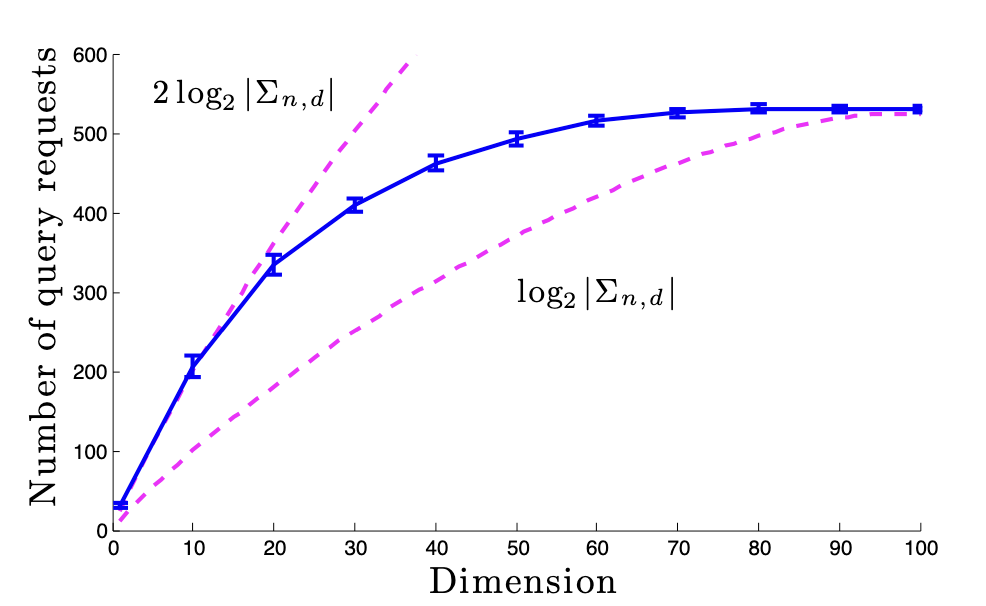
\includegraphics[width=0.6\textwidth,height=\textheight]{src/Figures/Dim:query_graph.png}

}

\caption{\label{fig-rand_n}Mean and standard deviation of requested
queries (solid) in the noiseless case for \(n = 100\);
\(\log_2|\Sigma_{n,d}|\) is a lower bound (dashed).}

\end{figure}%

\begin{longtable}[]{@{}llcc@{}}
\caption{Statistics for the Robust Query Selection Algorithm (RQSA)
(\citeproc{ref-geo_paper}{G. and Nowak 2011}) discussed at the end of
Section~\ref{sec-QSA} and the baseline of conducting all comparisons.
\(y\) serves as a noisy ground truth, \(\tilde{y}\) is the result of all
comparisons, and \(\hat{y}\) is the output of the
RQSA.}\label{tbl-geo_acc}\tabularnewline
\toprule\noalign{}
Dimension & & 2 & 3 \\
\midrule\noalign{}
\endfirsthead
\toprule\noalign{}
Dimension & & 2 & 3 \\
\midrule\noalign{}
\endhead
\bottomrule\noalign{}
\endlastfoot
\% of queries & mean & 14.5 & 18.5 \\
requested & std & 5.3 & 6 \\
Average error & \(d(\bar{y}, y)\) & 0.23 & 0.21 \\
& \(d(\bar{y}, y)\) & 0.31 & 0.29 \\
\end{longtable}

Figure~\ref{fig-rand_n} shows that the number of comparisons fits within
the expected bounds, as \(\log|\Sigma_{n,d}| = \log(n^d) = d\log n\). To
derive that graph, authors (\citeproc{ref-geo_paper}{G. and Nowak 2011})
sampled 100 random data points in a \(R^d\) space, where \(d\) took on
10 different values as indicated on the graph. Each dimension's
experiments were repeated 25 times for consistency.

With regard to the accuracy and performance of the method, the authors
did a ranking experiment on 100 different audio signals, results of
which can be seen in Table~\ref{tbl-geo_acc}. The ground truth labels
came from humans, indicated by \(y\) in the table. That resulted in the
existence of noise and potential errors in the ground truth, which could
influence the performance of both the baseline algorithm that does all
comparisons (\(\tilde{y}\)) and the Robust Query Selection Algorithm
(RQSA) proposed in Section~\ref{sec-QSA} (\(\hat{y}\)). As can be seen
in both 2 and 3-dimensional spaces RQSA performed worse by \(8\%\)
compared to the baseline, which indicates that active learning that uses
the domain information can still be erroneous due to the inference of
certain comparisons that sometimes may not be entirely correct. However,
as can be seen by the upper part of Table~\ref{tbl-geo_acc},
significantly less queries were requested compared to the baseline,
which means that the approach can have a significant benefit at a cost
of slight loss in accuracy.

\subsubsection{User Information as Domain Knowledge for Active
Learning}\label{sec-geo_app}

An alternative source of domain knowledge could be users themselves, who
can indicate their uncertainty when it comes to comparing two objects.
Prior studies have shown (\citeproc{ref-unnoisy_humans}{Amershi et al.
2014}) that when presented with only two options when selecting which
object is better, but not being able to properly decide, users would get
frustrated and tend to respond more faultyly, creating noise and
incorrect responses in the data. Through feedback and other studies
(\citeproc{ref-noisy_humans}{Guillory and Bilmes 2011}) it was
determined that presenting users with an option of indifference between
the two objects can remove those problems. Moreover, in connection to
active learning, the authors show that such an option helps to select
more informative queries since it provides more domain knowledge that
can be used, resulting in a decrease in the number of queries required.

For this problem, the following terms are defined:

\begin{enumerate}
\def\labelenumi{\arabic{enumi}.}
\item
  \(c\) - a cost function that represents user preferences, and the
  result the model has to determine at the end of training. The
  preferred items will have lower costs, and less preferred ones will
  have higher costs. The goal is to determine this function with the
  fewest possible number of queries using active learning.
\item
  \(H\) - a set of hypotheses over the possible cost functions, where
  for each \(h \in H\) there is a cost function \(c_h\) associated with
  it.
\item
  \(h^*\) - a true hypothesis that the model needs to determine, which
  has cost \(c_{h^*}\) associated with it
\item
  \(t(x,y)\) - a test performed to compare items \(x\) and \(y\) (the
  user is being asked to provide a response to which item is better).
  Those tests result in changes and adjustments to \(H\) as more
  information is learned.
\item
  \(o(x,y)\) - observation or result of \(t(x,y)\), where
  \(o(x,y) \in \{x<y, x>y\}\)
\item
  \(S = \{(t_1, o_1), (t_2, o_2),...,(t_m, o_m)\}\) - a sequence of
  \(m\) pairs of tests and observations
\item
  \(w(H|S)\) - probability mass of all hypotheses that are still
  consistent with the observations (similar to the dark grey area from
  Figure~\ref{fig-dim-space} and \(Q(i,j)\) discussed in
  Section~\ref{sec-QSA}. This means that if \(h \in H\) is inconsistent
  with user responses received, it is removed from \(H\).
\end{enumerate}

With the key terms defined, let's consider the noiseless base setting
where users only have two options for response. Those components will
also later be translated to the setting with the third option so the
true cost function can be determined there. \(w(H|S)\) is the sum of the
weights of all hypotheses that are still consistent with the evidence.
\[\begin{aligned}
    w(H|S) = \sum_{h \in H} w(h | S)\\
\end{aligned}\] Each \(w(h|S)\) is a probability of the evidence's
existence given such hypothesis: \[\begin{aligned}
    w(h|S) = p(S|h)
\end{aligned}\] Such probability comes from the test-observation pairs
since they compose the set \(S\). Moreover, each test is independent of
other tests, which gives: \[\begin{aligned}
    p(S|h) = \prod_{(t,o) \in S} p((t,o) | h)
\end{aligned}\] In the noiseless setting, users will select an option
that minimizes their cost function (selecting more preferred items),
mathematically defined as: \[\begin{aligned}
    p((t, o = x) | h) = 
    \begin{cases}
        1 & c_h(x) < c_h(y)\\
        0 & else
    \end{cases}
    \label{eq:prob_base}
\end{aligned}\]

\textbf{6.3.3.1 User Noise Modeling}

As has been discussed, users are not perfect evaluators and even get
frustrated if unable to select the better option. Prior work
(\citeproc{ref-unnoisy_humans}{Amershi et al. 2014}) has shown that
treating users as perfect can lead to poor performance. That gave rise
to accounting for noise in users' responses, but a majority of such work
applies the same noise to all queries and all responses. While those led
to great performance results (\citeproc{ref-noisy_humans}{Guillory and
Bilmes 2011}), they don't accurately reflect the real world, which gave
rise to the idea of creating query-based noise.

Effectively, for some of the queries it is important to incorporate the
fact that the user is unsure and noisy, but for others, if the user is
confident, noise in the response is not needed at all. For
comparison-based learning, this means that the noise is related to the
costs of the two items compared. Specifically for items \(x\) and \(y\),
if \(c_{h^*}(x) \simeq c_{h^*}(y)\) then the items are hard to
distinguish for the user, so here it is preferred to incorporate user
uncertainty and noise. But if \(c_{h^*}(x) >> c_{h^*}(y)\), the user
will certainly select \(y\) and the other way around, which is where the
noise is not needed.

Query-dependent noise is also supported in the psychology literature,
which means that such an approach is more related to the real world. In
particular, psychologists talk about the Luce-Sheppard Choice rule
(\citeproc{ref-lus-shep}{Shepard 1957}) when talking about comparisons.
This rule previously gave rise to a logistic model based on the noise
(\citeproc{ref-lus-log}{Viappiani and Boutilier 2010}) where the
probability of observation for a given test is: \[\begin{aligned}
    p((t, o = x) | h) \propto exp(-\gamma * c_h(x))
    \label{eq:noise_model}
\end{aligned}\]

\begin{figure}

\centering{

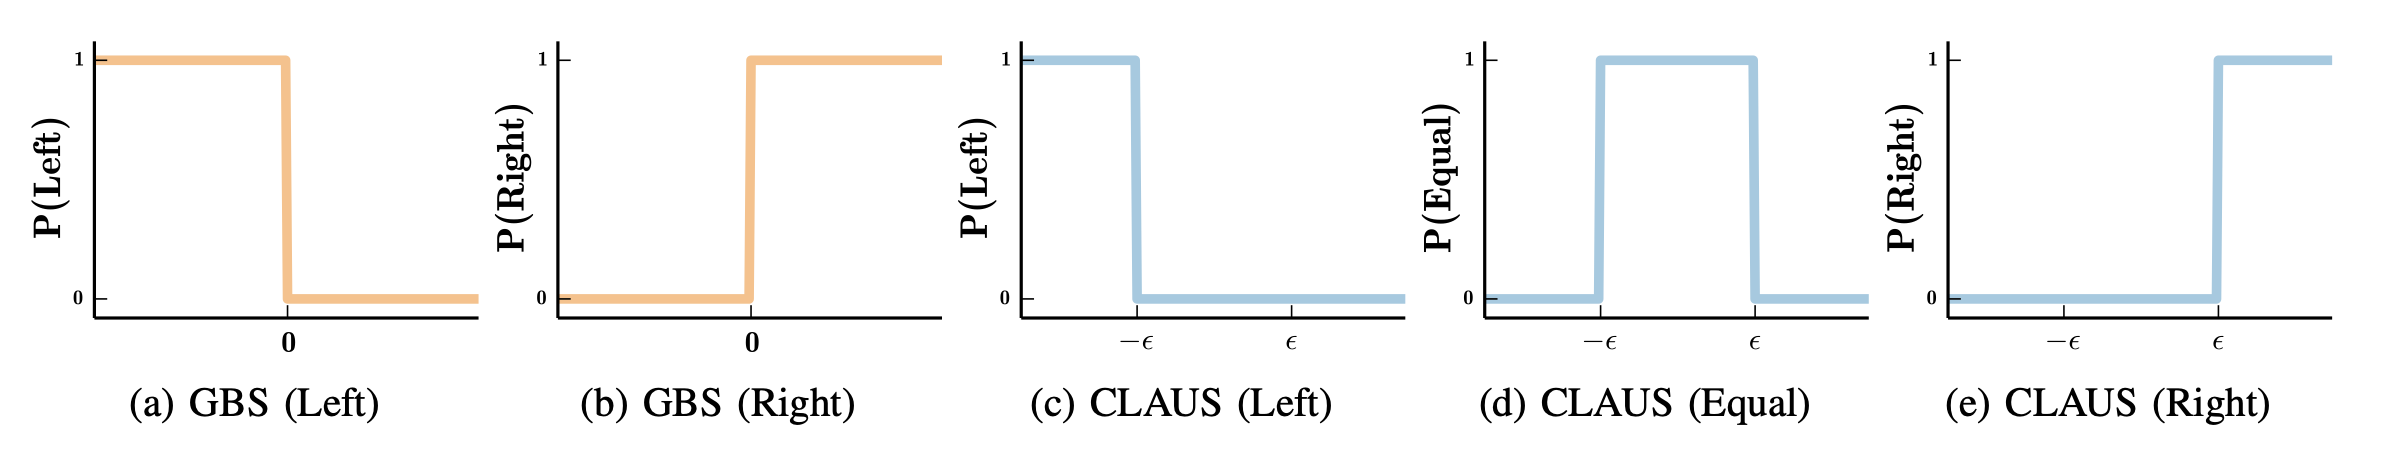
\includegraphics[width=1\textwidth,height=\textheight]{src/Figures/Noiseless probs.png}

}

\caption{\label{fig-noiseless_1}User response model in the noiseless
setting}

\end{figure}%

\begin{figure}

\centering{

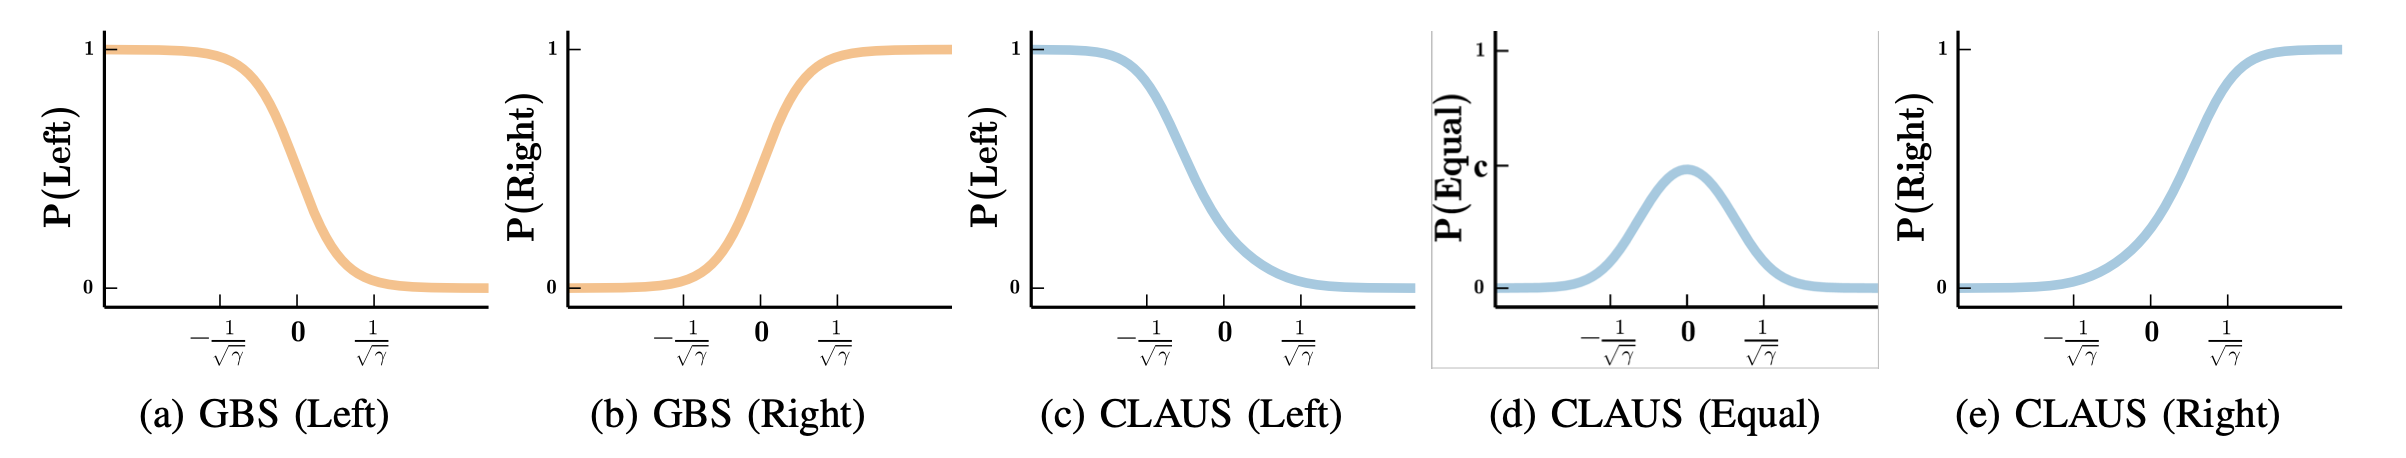
\includegraphics[width=1\textwidth,height=\textheight]{src/Figures/Noise probs.png}

}

\caption{\label{fig-noiseless_2}User response with Luce Sheppard noise
model}

\end{figure}%

Figure~\ref{fig-noiseless_1}, Figure~\ref{fig-noiseless_2} demonstrate
the difference between the noiseless setting and incorporating the
Luce-Sheppard Choice rule. GBS is the baseline model with only 2
response options, and CLAUS is the model with the uncertainty option
added. The figures show how incorporating such noise influences and
smoothes the probability distribution of the user's response.

\textbf{6.3.3.2 User Uncertainty}

We will now discuss the functionality of CLAUS, which is an algorithm
designed by (\citeproc{ref-claus}{Holladay et al. 2016}) that allows
users to select an uncertain response about the two options that they
need to rank. The authors model such uncertainty as \(\epsilon\) and it
is associated with each \(c_h\), so now every hypothesis \(h\) is
defined over a pair of \((c_h, \epsilon_h)\). It is important to note
that the goal is to still learn and maintain our objective on \(c\),
\(\epsilon\) is only necessary to model the users' responses. The
uncertainty relates to the cost function in the following way:
\[\begin{aligned}
    |c_h(x) - c_h(y)| < \epsilon_h
\end{aligned}\] this means that the user is uncertain between items
\(x\) and \(y\) and their cost difference is negligible such that the
user is not able to select which item is better. This in turn gives more
information about the real value of the two items, as a binary response
would indicate the user's preference towards one item, which will not be
real and will skew the cost functions.

This causes modifications of the problem set-up:

\begin{enumerate}
\def\labelenumi{\arabic{enumi}.}
\item
  For test \(t(x,y)\) the observation will be
  \(o(x,y) \in \{x<y, x>y, \tilde{xy}\}\), where \(\tilde{xy}\) is the
  uncertain response.
\item
  The probability distribution over the user's response
  \hyperref[eq:prob_base]{{[}eq:prob\_base{]}} will now be defined as:
  \[\begin{aligned}
  p((t, o = x) | h) = 
  \begin{cases}
      1 & c_h(x) < c_h(y) - \epsilon_h\\
      0 & else
  \end{cases}
  \end{aligned}\]
\end{enumerate}

\[\begin{aligned}
    p((t, o = \tilde{xy}) | h) = 
    \begin{cases}
        1 & |c_h(x) - c_h(y)|^2 < \epsilon_h^2\\
        0 & else
    \end{cases}
\end{aligned}\]

\begin{verbatim}
This means the user confidently selects $x$ when it
is better than $y$ by more than $\epsilon$, but if the squared
difference of the cost functions of two items is negligible by
$\epsilon$ user will choose the indifferent option.
\end{verbatim}

\begin{enumerate}
\def\labelenumi{\arabic{enumi}.}
\setcounter{enumi}{2}
\tightlist
\item
  Finally this also updates the noise model
  \hyperref[eq:noise_model]{{[}eq:noise\_model{]}}: \[\begin{aligned}
  p((t, o = x) | h) \propto \exp(-\gamma * [c_h(x) - c_h(y)])
  \end{aligned}\]
\end{enumerate}

\[\begin{aligned}
    p((t, o = \tilde{xy}) | h) \propto exp(-1/\epsilon_h^2 * [c_h(x) - c_h(y)]^2)
\end{aligned}\]

\textbf{6.3.3.3 Performance Analysis}

\begin{figure}

\centering{

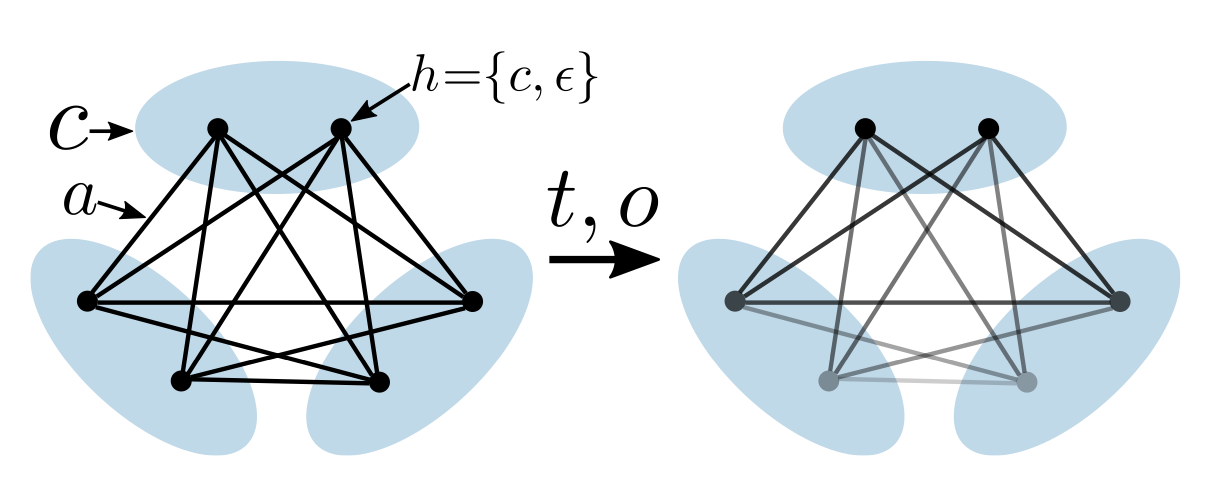
\includegraphics[width=0.6\textwidth,height=\textheight]{src/Figures/equiv.png}

}

\caption{\label{fig-equiv_c}CLAUS using equivalence classes. Each cost
function \(c\) corresponds to an equivalence class (blue ellipse).
Hypotheses (black dots) are \(\{c_h,\epsilon_h\}\) pairs. Hypotheses
sharing a cost \(c\) are said to be inside the equivalence class of
\(c\). After performing a test and receiving an observation, the
evidence results in downweighting connections among some of the
hypotheses.}

\end{figure}%

Before diving deeper into the comparisons of performance, it is
important to indicate that rather than predicting a specific pair
\((c_h, \epsilon_h)\), the algorithm focuses on predicting a group of
pairs that are similar to one another, otherwise called equivalence
class (Figure~\ref{fig-equiv_c}), which indicates not essentially
different hypothesis for the cost function and uncertainty. That
information is learned through each new test, as the algorithm updates
the information about \(c\) and \(\epsilon\) that distinguishes between
the distinct \(h\), finding the equivalence groups among them. Moreover,
the authors tweaked the parameter responsible for the size of the
equivalence class (how many hypotheses can be grouped together at a
time).

\begin{figure}

\centering{

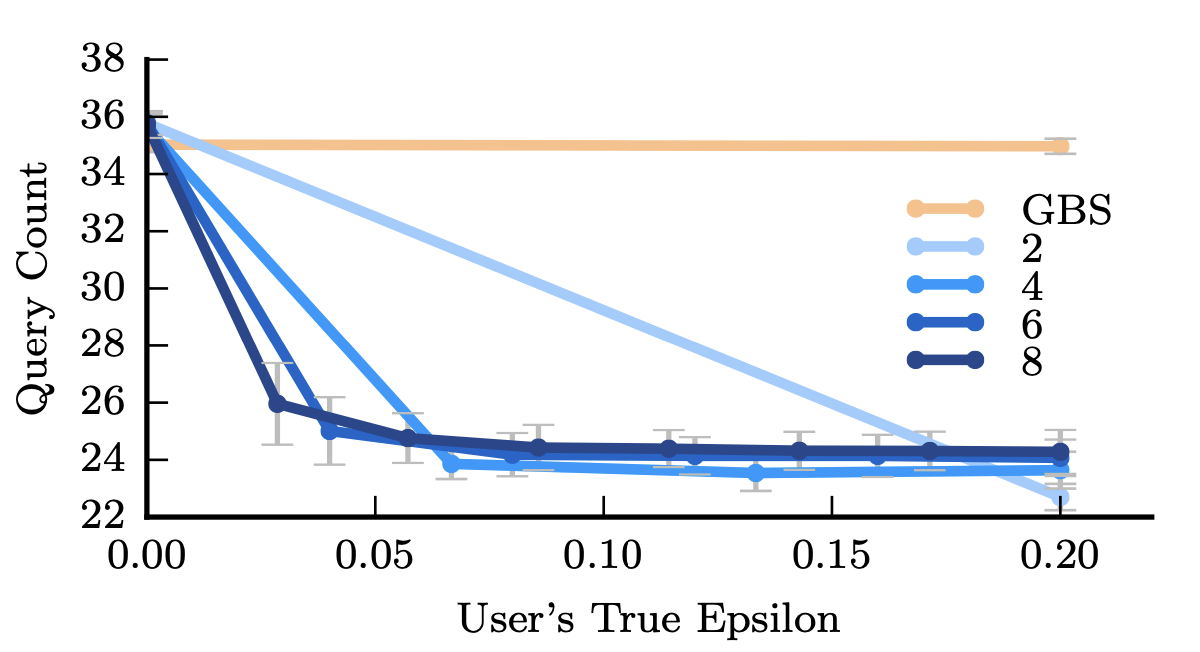
\includegraphics[width=0.6\textwidth,height=\textheight]{src/Figures/GBS:CLAUS.png}

}

\caption{\label{fig-claus_num}Performance of GBS and its variants}

\end{figure}%

\begin{longtable}[]{@{}lcc@{}}
\caption{Performance of GBS and CLAUS with different labels for the
uncertainty}\label{tbl-claus_tab}\tabularnewline
\toprule\noalign{}
Category & Accuracy & Query Count \\
\midrule\noalign{}
\endfirsthead
\toprule\noalign{}
Category & Accuracy & Query Count \\
\midrule\noalign{}
\endhead
\bottomrule\noalign{}
\endlastfoot
GBS - About Equal & \(94.15 \pm 0.52\) & \(36.02 \pm 0.03\) \\
GBS - Not Sure & \(\textbf{94.66} \pm \textbf{0.55}\) &
\(35.95 \pm 0.04\) \\
CLAUS - About Equal & \(91.56 \pm 0.84\) &
\(\textbf{25.93} \pm \textbf{0.41}\) \\
CLAUS - Not Sure & \(90.86 \pm 0.74\) & \(26.98 \pm 0.47\) \\
\end{longtable}

The first performance evaluation is done on the number of queries and
confirms that it decreases in Figure~\ref{fig-claus_num}. The GBS model
serves as the baseline, as it will do all of the comparison queries
using the binary response options. The CLAUS model is measured over
different values of \(\epsilon\) on the x-axis and over different sizes
of the equivalence sets indicated by different shades of blue. Figure
shows that all variants of CLAUS use approximately 10 fewer queries on
average compared to GBS. Moreover, using bigger-sized equivalence
classes can further decrease the number of needed queries. The most
optimal \(\epsilon \simeq 0.07\), after which higher \(\epsilon\) does
not provide any benefit.

Lastly, the authors considered the performance difference, which is
indicated in Table~\ref{tbl-claus_tab}. For that authors used two
different labels for the uncertainty button in CLAUS, it was either
labeled as "About Equal" or "Not Sure" as those can provoke different
responses and feelings in users. Moreover, GBS and CLAUS-type responses
were mixed in the same set of questions to the user, which splits the
metrics for both in two as can be seen in Table~\ref{tbl-claus_tab}. The
performance of CLAUS is lower by \(3\%\) on average, indicating similar
results to Section~\ref{sec-geo_app}, showing that a smaller number of
queries can still lead to a performance loss. However, the second column
of Table~\ref{tbl-claus_tab} supports the information in
Figure~\ref{fig-claus_num}, as it also shows that 10 fewer queries were
conducted on average.

\subsection{Active Preference-Based Learning of Reward
Functions}\label{active-preference-based-learning-of-reward-functions}

Active learning can be essential in learning within dynamic systems and
environments. Say we have an agent in an environment, and we want it to
conform to a certain behavior as set by a human. How exactly do we go
about doing this? In a traditional RL setting, this is solved by a class
of algorithms under Inverse Reinforcement Learning. Techniques such as
VICE and GAIL attempt to learn a reward function that can distinguish
between states visited by the agent and states desired to be visited as
defined by a human. In effect, a human will demonstrate what it would
like the agent to do in the environment, and from there, learning is
done. However, what if humans do not precisely know how an agent should
optimally behave in an environment but still have some opinion on what
trajectories would be better than others? This is where a paper like
Active Preference-Based Learning of Reward Functions comes into the
picture. The paper aims to use human preferences to aid an agent's
learning within a dynamic system.

A dynamic system contains human input, robotic input, and an environment
state. The transitions between states is defined by \(f_{HR}\), so that
we have: \[x^{t+1} = f_{HR}(x^t, u_R, u_H)\] At a given time step \(t\),
we have \(x_t\), \(u_R^t\), and \(u_H^t\). This can be encapsulated into
a single \(d\) dimensional feature vector that the authors denote as
\(\phi\). The paper then assumes that the underlying reward model we are
trying to learn can be represented linearly. If we have our human reward
preference function defined as \(r_H\), this means we can write \(r_H\)
as: \[r_H(x^t, u_R^t, u_H^t) = w^{\intercal}\phi(x^t, u_R^t, u_H^t)\]
Because the reward function is linear, we can take the weight vector out
of the summation if we want to calculate the reward over an entire
trajectory:
\[R_{H}(x^0, u_R, u_H) = \sum_{t=0}^{N} r_{H}(x^t, u^t, u_H^t)\]
\[\Phi = \sum \phi(x^t, u_R^t, u_H^t)\] \[R_H(traj) = w\cdot\Phi(traj)\]

\subsubsection{Properties of W}\label{properties-of-w}

First, the scale of \(w\) does not matter because we only care about the
relative rewards produced with \(w\) (given two different trajectories,
we want to answer the question of which trajectory a human would prefer,
i.e.~which one has a higher preference reward). This means we can
constrain \(||w|| <= 1\), so the initial prior is uniform over a unit
ball. From here, we can determine a probabilistic expression to assess
whether we should prefer trajectory A or B (because it can be noisy with
human input). Let \(I_t = +1\) if the human prefers trajectory \(A\) and
let \(I_t = -1\) if the human prefers trajectory \(B\). We get the
following for \(p(I_t | w)\).

\[p(I_t = +1|w) = \frac{exp(R_H(traj_A))}{exp(R_H(traj_A)) + exp(R_H(traj_B)}\]
\[p(I_t = -1|w) = \frac{exp(R_H(traj_B))}{exp(R_H(traj_A)) + exp(R_H(traj_B)}\]

We can re-write this expression to make it cleaner, using the following
substitution: \[\psi = \Phi(traj_a) - \Phi(traj_b)\]
\[f_{\psi} (w) = p(I_t|w) = \frac{1}{1 + exp(-I_tw^{\intercal}\psi}\]

The idea now is that we can update \(p(w)\) everytime we get a result
from a human preference query using Bayes:

\[p(w|I_t) <- p(w) \cdot p(I_t|w)\]

We don't need to know \(p(I_t)\) because we can use an algorithm like
the Metropolis algorithm to actually sample.

\subsubsection{Generating Queries}\label{generating-queries}

This is where the interesting part of the paper comes into play. How do
we actually generate queries for the user to pick between? This paper
synthetically generates queries through an optimization process and then
presents them to a human to pick between. The idea is that we want to
generate a query that maximizes the conditional entropy \(H(I|w)\).
There are a few ways to think about this -- intuitively we want to pick
a query that we are most uncertain about given our current weights (thus
having the highest conditional entropy given the weights). The way the
authors of the paper frame this originally in the paper is that "we want
to find the next query such that it will help us remove as much volume
(the integral of the unnormalized pdf over w) as possible from the space
of possible rewards." Mathematically this can be written as:

\[max_{x^0, u_R, u_H^A, u_H^B} min\{E[1-f_{\psi}(w)], E[1 - f_{-\psi}(w)]\}\]

But how exactly do we optimize this expression mathematically? After
all, we need to use this expression to generate synthetic queries. The
answer is to sample \(w_1, ... w_m\) from \(p(w)\). We can assume we are
sampling points from a point cloud, thus approximating the distribution
\(p(w)\) as

\[p(w) = \frac{1}{M} \sum \delta (w_i)\]. We can now approximate the
expectation expression like so:
\[E[1 - f_{\psi}(w)] = \frac{1}{M} (\sum 1 - f_{\psi}(w_i))\]

and now we can optimize the expression to generate a synthetic query!
Altogether, the algorithm looks like the following:

\textbf{input:} features \(\phi\), horizon \(N\), dynamics \(f\),
\(iter\) \textbf{initialize:} \(p(w) \sim Uniform(B)\), for a unit ball
\(B\) \(W \gets M\) samples from \(AdaptiveMetropolis(p(w))\)
\((x^0, u_R, u^A_H, u^B_H) \gets SynthExps(W,f)\)
\(I_t \gets QueryHuman(x^0, u_R, u^A_H, u^B_H)\)
\(\varphi = \Phi(x^0, u_R, u^A_H) - \Phi(x^0, u_R, u^B_H)\)
\(f_\varphi(w) = \min(1, I_t\exp(w^\top \varphi))\)
\(p(w) \gets p(w) \cdot f_\varphi(w)\) \(t \gets t+1\) \textbf{output:}
distribution of \(w: p(w)\)

\subsubsection{Batching Queries}\label{batching-queries}

The algorithm itself works well, however there ends up being a bottle
neck that each query needs to be synthesized before being sent to the
human -- one at a time. In other words, the human gives their feedback,
waits for a query to be synthesized, and then gives another data point
of feedback. There is no room for parallelization and so the authors
proposed a second algorithm in a separate paper that allows for the
batching of queries. Simply put, we change the mathematical expression
to the following:

\[max_{\xi_{ib+1_A}, \xi_{ib+1_B}, ... , \xi_{ib+b_A}, \xi_{ib+b_B} H(I_{ib+1}, I_{ib+2}, .., I_{ib+b} | w)}\]

Naively, we could consider optimizing this in the greedy fashion. This
would mean just synthetically generating \(b\) independent queries. The
obvious drawback of this method would be that the queries would likely
be very similar to each other. The authors propose a few other
heuristics that would help guide the algorithm away from generating very
similar queries. As an example, the authors propose Medioid Selection
where we have to cluster \(B\) greedy vectors into \(b < B\) groups and
pick one vector from each group (the medioid). The authors also propose
two other methods rooted in providing different queries: boundary
medioids selection and successive elimination. They are best visually
depicted as:

\begin{figure}

\centering{

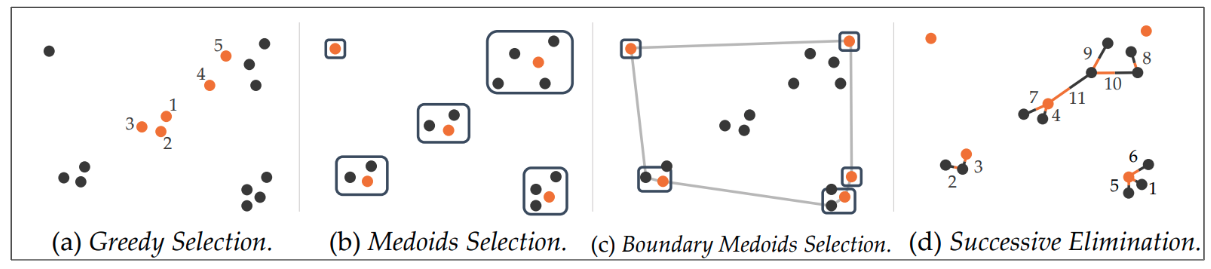
\includegraphics[width=0.75\textwidth,height=\textheight]{src/Figures/greedy.png}

}

\caption{\label{fig-selection-strategy}Different selection strategies}

\end{figure}%

\subsubsection{Results}\label{results}

The authors test both the non-batched and variety of batched learning
algorithms on multiple environments:

\begin{figure}

\centering{

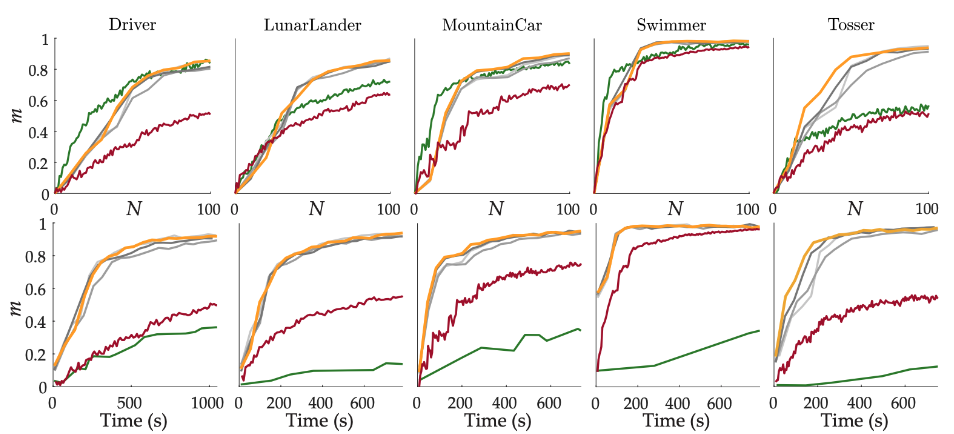
\includegraphics[width=0.75\textwidth,height=\textheight]{src/Figures/activeresults.png}

}

\caption{\label{fig-batch-nonbatch}Comparison between batched and
non-batched algorithms}

\end{figure}%

What is interesting to note is that when graphed over \(N\) the
non-batched active learning approach does in the same ball-park of
performance as the batched approaches. However, if you graph it over
time, we see that learning is a much slower process when not-batched.

\section{Foundation Models for
Robotics}\label{foundation-models-for-robotics}

Modern foundation models have been ubiquitous in discussions of
powerful, general purpose AI systems that can accomplish myriad tasks
across many disciplines such as programming, medicine, law, open
question-answering and much more, with rapidly increasing capabilities
(\citeproc{ref-bommasani2022opportunities}{Bommasani et al. 2022}).
However, despite successes from large labs in controlled environments
(\citeproc{ref-brohan2023rt2}{Brohan et al. 2023}) foundation models
have not seen ubiquitous use in robotics due to shifting robot
morphology, lack of data, and the sim to real gap in robotics
(\citeproc{ref-walke2023bridgedata}{Walke et al. 2023}). For this
subsection we explore two promising approaches known as R3M and Voltron
which are the first to leverage pre-training on vast amounts of data
towards performance improvement on downstream robotic tasks despite the
aforementioned issues (\citeproc{ref-nair2022r3m}{Nair et al. 2022};
\citeproc{ref-karamcheti2023languagedriven}{Karamcheti et al. 2023}).

\subsection{R3M: Universal Visual Representation for
Robotics}\label{r3m-universal-visual-representation-for-robotics}

\begin{figure}

\centering{

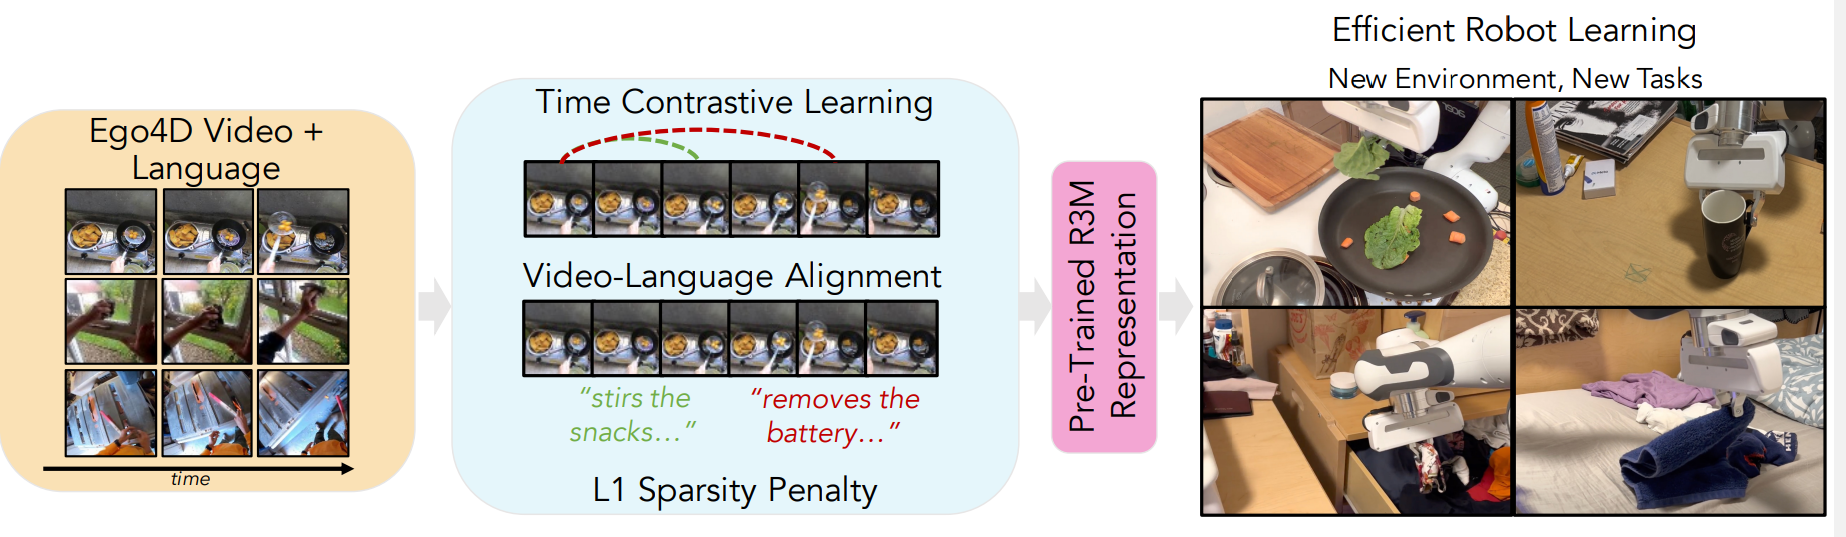
\includegraphics[width=0.95\textwidth,height=\textheight]{src/Figures/r3m.png}

}

\caption{\label{fig-r3m-pipline}R3M pipeline}

\end{figure}%

R3M represents a significant advancement in the field of robotic
manipulation and learning. This model diverges from traditional
approaches that rely on training from scratch within the same domain on
the same robot data as instead it leverags pretraining on large
datasets, akin to the practices in computer vision and natural language
processing (NLP) where models are trained on diverse, large-scale
datasets to create reusable, general-purpose representations.

The core principle behind R3M is its training methodology. It is
pre-trained on a wide array of human videos, encompassing various
activities and interactions. This diverse dataset enables the model to
capture a broad spectrum of physical interactions and dynamics, which
are crucial for effective robotic manipulation known as EGO4D
(\citeproc{ref-grauman2022ego4d}{Grauman et al. 2022}). However, prior
papers could not fit this dataset well, and R3M leveraged. The training
utilizes a unique objective that combines time contrastive learning,
video-language alignment, and a sparsity penalty. This objective ensures
that R3M not only understands the temporal dynamics of scenes (i.e., how
states transition over time) but also focuses on semantically relevant
features, such as objects and their interrelations, while maintaining a
compact and efficient representation.

What sets R3M apart in the realm of robotics is its efficiency and
effectiveness in learning from a limited amount of data. The model
demonstrates remarkable performance in learning tasks in the real world
with minimal human supervision -- typically less than 10 minutes. This
is a stark contrast to traditional models that require extensive and
often prohibitively large datasets for training. Furthermore, R3M's
pre-trained nature allows for its application across a variety of tasks
and environments without the need for retraining from scratch, making it
a versatile tool in robotic manipulation. The empirical results from
using R3M are compelling, leading to a 10\% improvement over training
from a pretrained image-net model, self-supervised approaches such as
MoCo or even CLIP (\citeproc{ref-deng2009imagenet}{Deng et al. 2009};
\citeproc{ref-he2020momentum}{He et al. 2020};
\citeproc{ref-radford2021learning}{Radford et al. 2021}). Note however,
that R3m does \textbf{not} use any language data which leaves quite a
bit of supervision to be desired.

\subsection{Voltron: Language Driven Representation Learning for
Robotics}\label{voltron-language-driven-representation-learning-for-robotics}

Building off the success of R3M, Voltron proposes a further extension of
leveraging self-supervision and advancements in foundation models, and
multi-modality. Voltron takes on an intuitive and simple dual use
objective, where the trained model alternates between predicting the
task in an image through natural language and classifying images based
on a natural text label. This forces a nuanced understanding of both
modalities (\citeproc{ref-radford2021learning}{Radford et al. 2021}).

Voltron's approach is distinguished by its versatility and depth of
learning. It is adept at handling a wide range of robotic tasks, from
low-level spatial feature recognition to high-level semantic
understanding required in language-conditioned imitation and intent
scoring. This flexibility makes it suitable for various applications in
robotic manipulation, from grasping objects based on descriptive
language to performing complex sequences of actions in response to
verbal instructions.

\begin{figure}

\centering{

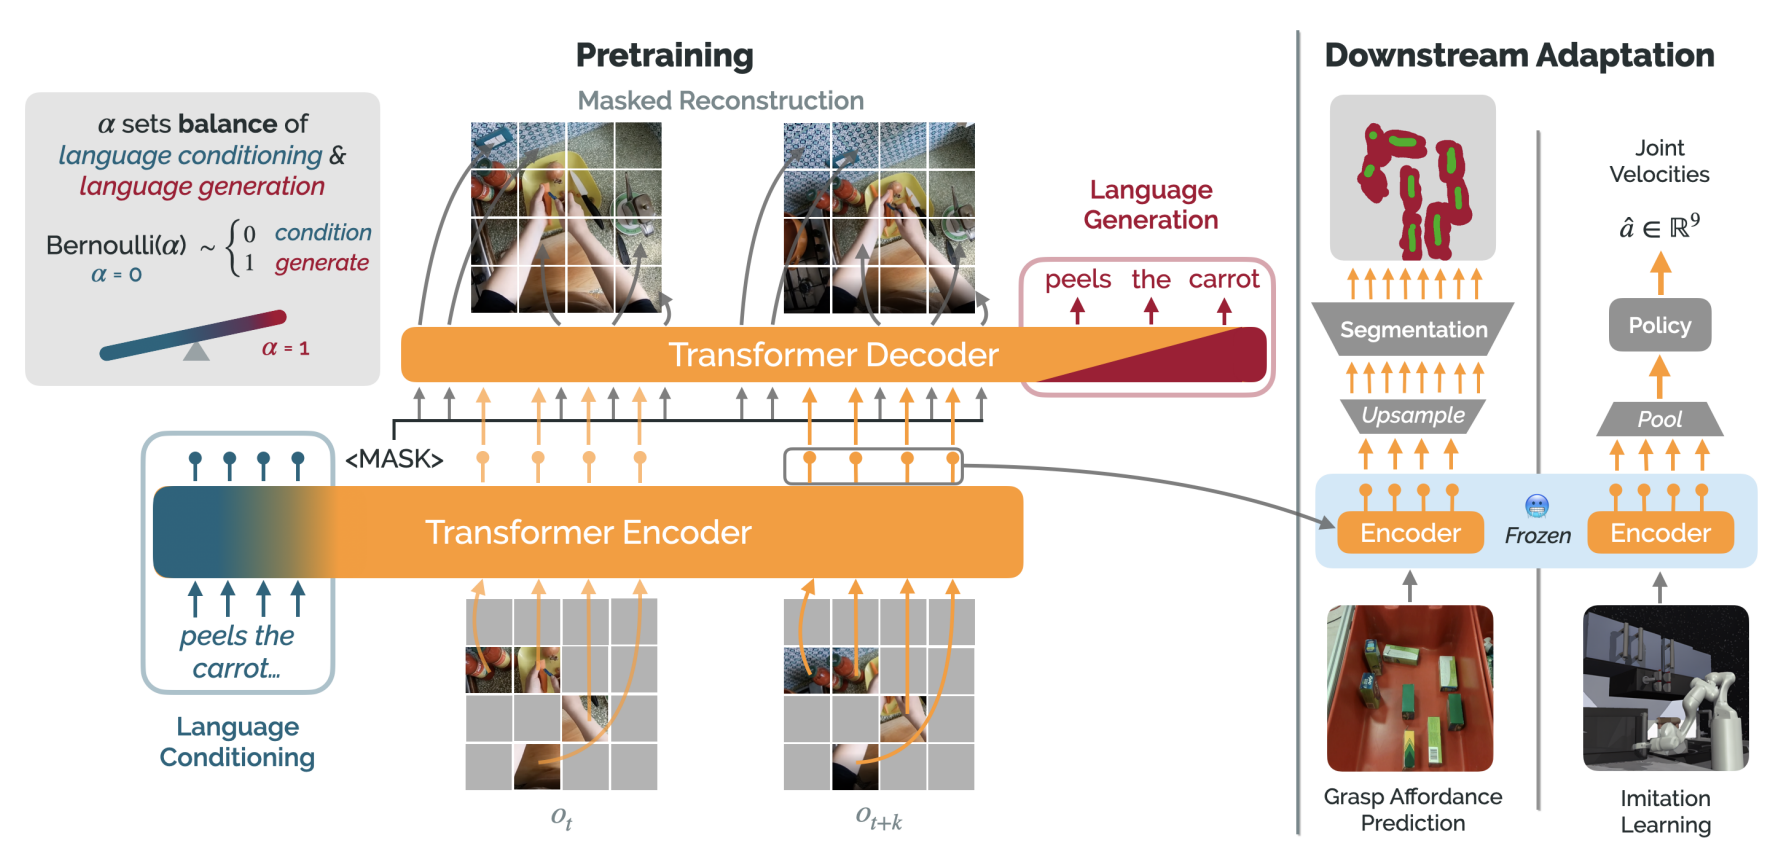
\includegraphics[width=0.95\textwidth,height=\textheight]{src/Figures/voltron.png}

}

\caption{\label{fig-voltron-pipeline}Voltron pipeline}

\end{figure}%

The authors rigorously test Voltron in scenarios such as dense
segmentation for grasp affordance prediction, object detection in
cluttered scenes, and learning multi-task language-conditioned policies
for real-world manipulation with up to 15\% improvement over baselines.
In each of these domains, Voltron has shown a remarkable ability to
outperform existing models like MVP and R3M, showcasing its superior
adaptability and learning capabilities
(\citeproc{ref-xiao2022masked}{Xiao et al. 2022}).

Moreover, Voltron's framework allows for a balance between encoding
low-level and high-level features, which is critical in the context of
robotics. This balance enables the model to excel in both control tasks
and those requiring deeper semantic understanding, offering a
comprehensive solution in the realm of robotic vision and manipulation.

Voltron stands as a groundbreaking approach in the field of robotics,
offering a language-driven, versatile, and efficient approach to
learning and manipulation. Its ability to seamlessly integrate visual
and linguistic data makes it a potent tool in the ever-evolving
landscape of robotic technology, with potential applications that extend
far beyond current capabilities. Interesting the authors show Voltron
does not beat R3M off the shelf but only when trained on similar amounts
of data. Nevertheless, Voltron's success in diverse tasks and
environments heralds a new era in robotic manipulation, where language
and vision coalesce to create more intelligent, adaptable, and capable
robotic systems.

\section{Conclusion}\label{conclusion}

On the note of applying active learning to RL and environment settings,
there have been many recent papers that have attempted to extend this to
more modern RL environments. For example, the paper "When to Ask for
Help" (\citeproc{ref-ask_help}{Xie et al. 2022}) examines the
intersection of autonomous and active learning. Instead of just
expecting an RL agent to autonomously solve a task, making the
assumption that an agent could get stuck and need human input to get
"unstuck" is a key insight of the paper. In general, there has been an
emphasis in recent literature in robotics on not just blindly using
demonstration data as a form of human input, but rather actively
querying a human and using this to better synthesize correct actions.

Active learning holds promise for enhancing AI models in real-world
scenarios, yet several challenges persist. This discussion aims to
provide an overview of these challenges.

\textbf{Task-Specific Considerations:}

For certain tasks, the input space of a model may have some rare yet
extremely important pockets which may never be discovered by active
learning and may cause severe blindspots in the model. In medical
imaging for instance, there can be rare yet critical diseases. Designing
AL strategies for medical image analysis must prioritize rare classes,
such as various forms of cancers. Oftentimes, collecting data around
those rare classes is not a recommendation of the active learning
process because these examples constitute heavy distribution drifts from
the input distribution a model has seen.

\textbf{Complex Task Adaptation:}

AL has predominantly been adopted for simple classification tasks,
leaving more other types of tasks (generative ones for instance), less
explored. In Natural Language Processing, tasks like natural language
inference, question-answering pose additional complexities that affect
the direct application of the active learning process. While machine
translation has seen AL applications, generation tasks in NLP require
more thorough exploration. Challenges arise in obtaining unlabeled data,
particularly for tasks with intricate inputs.

\textbf{Unsupervised and Semi-Supervised Approaches:}

In the presence of large datasets without sufficient labels,
unsupervised and semi-supervised approaches become crucial. These
methods offer a means to extract information without relying on labeled
data for every data point, potentially revolutionizing fields like
medical image analysis. There is an ongoing need for methods that
combine self/semi-supervised learning with active learning.

\textbf{Algorithm Scalability:}

Scalability is a critical concern for online AL algorithms, particularly
when dealing with large datasets and high-velocity data streams. The
computational demands of AL can become prohibitive as data volume
increases, posing challenges for practical deployment. Issues of
catastrophic forgetting and model plasticity further complicate
scalability, requiring careful consideration in algorithm design.

\textbf{Labeling Quality Assurance:}

The effectiveness of most online AL strategies hinges on the quality of
labeled data. Ensuring labeling accuracy in real-world scenarios is
challenging, with human annotators prone to errors, biases, and diverse
interpretations. Addressing imperfections in labeling through
considerations of oracle imperfections becomes essential in real-life AL
applications. Solutions for cleaning up data and verifying its quality
need to be more aggressively pursued.

\textbf{Data Drift Challenges:}

Real-world settings introduce data drift, where distributions shift over
time, challenging models to adapt for accurate predictions. These shifts
can impact the quality of labeled data acquired in the AL process. For
example, the criterion or proxy used for selecting informative instances
may be thrown off when the distribution a model is trained on, and the
distribution we want it to perform well on, are too far away from one
another.

\textbf{Evaluation in Real-Life Scenarios}:

While AL methods are often evaluated assuming access to ground-truth
labels, the real motivation for AL lies in label scarcity. Assessing the
effectiveness of AL strategies becomes challenging in real-life
scenarios where ground-truth labels may be limited. In other words, one
may verify the goodness of an AL algorithm within the lab, but once the
algorithm is deployed for improving all sorts of models on all sorts of
data distributions, verifying whether AL is actually improving a model
is tricky, especially when collecting and labeling data from the target
distribution is expensive and defeats the purpose of using AL in the
first place.

By systematically addressing these challenges, the field of active
learning in AI can progress towards more effective and practical
applications.

In summary, active learning is a promising modern tool to model training
that presents potential benefits. As was mentioned at the start, there
are numerous approaches that can be employed by active learning,
starting from reducing error of model's prediction, reducing variance,
to more conformal predictions. The flavor of active learning heavily
depends on the applications, which include robotics, LLM, autonomous
vehicles, and more. We discussed in more detail how to perform active
learning for variance reduction in the case of predicting kinematics of
the robotic arms, which showed decrease in MSE as well as more stable
reduction in it. Next we talked about using active learning for reducing
the number of comparisons required to create a ranking of objects, and
the examples discussed were able to achieve that but with some loss in
the prediction accuracy. Finally, we discussed how active learning can
be used for modeling of reward functions within a dynamical system,
which demonstrated improvements in performance and time required to
achieve it. For a more hands-on experience with active learning and
demonstrated example, we encourage the readers to explore a blogpost by
Max Halford (\citeproc{ref-max_halford}{Halford 2023}).

\section{Introduction to Performance Metric
Elicitation}\label{introduction-to-performance-metric-elicitation}

In binary classification problems, one important consideration is the
selection of an appropriate performance metric corresponding to the
real-world task at hand. The problem of \emph{metric elicitation}
attempts to characterize and discover the performance metric of a
practitioner, reflecting the rewards or costs that come with correct or
incorrect classification. For example, in medical contexts such as
diagnosing a disease or choosing whether a given treatment is
appropriate for a certain condition, tradeoffs are made for incorrect
decisions; for example, not administering a treatment could lead to the
worsening of a disease (a false negative), whereas delivering the wrong
kind of treatment could lead to adverse side effects that would be worse
than not treating the condition (a false positive).

Rather than choosing from a limited set of default choices like the
F1-score or weighted accuracy, metric elicitation considers the process
by which we can devise a metric that best matches the preferences of the
practitioners or users, by querying an ``oracle" who provides feedback
on proposed potential metrics in the form of pairwise comparisons.
Because queries to humans are often expensive, the aim is to minimize
the amount of comparisons needed.

\textbf{Note:} Almost all of the content in this chapter comes from
``Performance Metric Elicitation from Pairwise Classifier Comparisons''
by Hiranandani et al.
(\citeproc{ref-pmlr-v89-hiranandani19a}{Hiranandani et al. 2019a}),
which introduced the problem of metric elicitation and the framework for
binary-class metric elicitation from pairwise comparisons. In this
chapter, we aim to present their work expository while providing
additional motivation and intuitive explanations to supplement their
work.

The motivation for the pairwise comparison portion of metric elicitation
comes from a rich history of literature in psychology, economics, and
computer science (\citeproc{ref-pref1}{Samuelson 1938};
\citeproc{ref-pref2}{Mas-Colell 1977}; \citeproc{ref-pref3}{Varian
2006}; \citeproc{ref-pref4}{Braziunas and Boutilier 2012};
\citeproc{ref-ab}{Tamburrelli and Margara 2014}) demonstrating that
humans are often ineffective at providing absolute feedback on things
like potential prices, user interfaces, or even ML model outputs (hence
the comparison-based structure of RLHF, for instance). In addition,
confusion matrices are a way to accurately capture binary metrics such
as accuracy, \(F_\beta\), and Jaccard similarity by recording the number
of false positives, true positives, false negatives, and true negatives
obtained by a certain classifier. The main goal of this chapter is to
introduce two binary-search procedures that can be used to approximate
the oracle's performance metric for two types of metrics (linear and
linear-fractional performance metrics) by presenting the oracle with
confusion matrices generated by various classifiers; in essence, we are
learning an optimal threshold for classification given a decision
boundary for a binary classification problem.

First, we introduce some relevant notation that will later be used to
formalize notions of oracle queries, classifiers, and metrics.

\begin{itemize}
\item
  \(X \in \mathcal{X}\) is an input random variable.
\item
  \(Y \in \{0, 1\}\) is the output random variable.
\item
  We learn from a dataset of size \(n\), denoted by
  \(\{(x, y)_i\}^n_{i=1}\), generated iid from some distribution
  \(\mathbb{P}(X, Y)\).
\item
  \(\eta(\vec{x}) = \mathbb{P}(Y=1 | X=x)\) is the conditional
  probability of the positive class, given some sample \(x\).
\item
  \(\zeta = \mathbb{P}(Y=1)\) is the unconditional probability of the
  positive class
\item
  The set of all potential classifiers is
  \(\mathcal{H} = \{h : \mathcal{X} \rightarrow \{0,1\}\}\)
\item
  The confusion matrix for some classifier \(h\) is
  \(C(h, \mathbb{P}) \in \mathbb{R}^{2 \times 2}\), where
  \(C_{ij}(h, \mathbb{P}) = \mathbb{P}(Y=i, h=j)\) for
  \(i, j \in \{0,1\}\); these represent the false positives, true
  positives, false negatives, and true negatives, so
  \(\sum_{i,j}C_{ij}=1\).
\item
  \(\mathcal{C}\) is the set of all confusion matrices
\item
  Note: Since \(FN(h, \mathbb{P}) =\zeta - TP(h, \mathbb{P})\) and
  \(FP(h, \mathbb{P}) = 1 - \zeta - TN(h, \mathbb{P})\); \(\mathcal{C}\)
  is in fact a 2-dimensional space, not a 4-dimensional space
\item
  Any hyperplane (line) in \((tp, tn)\) given by
  \(\ell := a \cdot tp + b \cdot tn = c; a, b, c\in \mathbb{R}\)
\item
  Given a classifier \(h\), we define a performance metric
  \(\phi : [0, 1]^{2 \times 2} \rightarrow \mathbb{R}\). We refer to the
  value \(\phi(C(h))\), which represents the performance of a certain
  classifier with respect to a certain metric, as the \emph{utility} of
  the classifier \(h\). We assume, without loss of generality, that a
  higher value of \(\phi\) means \(h\) is a better performance metric.
\end{itemize}

Our focus is to recover some metric \(\phi\) using comparisons between
confusion matrices \(C(h)\), determined by classifiers \(h\), which
comes close to the oracle's ``ground-truth" metric \(\phi^*\).

Next, we introduce two classes of performance metrics, for which we will
present two elicitation algorithms. A \emph{linear performance metric
(LPM)}, given some constants
\(\{a_{11}, a_{01}, a_{10}, a_{00}\} \in \mathbb{R}^{4}\), is of the
form \[\begin{aligned}
\phi(C) & = a_{11} T P + a_{01} F P + a_{10} F N + a_{00} TN  = m_{11} T P + m_{00} T N + m_{0},
\end{aligned}\] where \(m_{11} = (a_{11} - a_{10})\),
\(m_{00} = (a_{00} - a_{01})\), and
\(m_{0} = a_{10} \zeta + a_{01} (1 - \zeta)\); the second line is a
useful parametrization of the metric, constructed using our observation
about the dimensionality of \(\mathcal{C}\). For example, one common LPM
is weighted accuracy: \(WA = w_1TP + w_2TN\), where varying the
proportion between \(w_1\) and \(w_2\) corresponds to different
importances afforded to various types of misclassification.

A slightly more complicated class of metrics are the
\emph{Linear-Fractional Performance Metrics (LFPM)}; given constants
\(\{a_{11}, a_{01}, a_{10}, a_{00}, b_{11}, b_{01}, b_{10}, b_{00}\} \in \mathbb{R}^{8}\),
an LFPM is defined as: \[\begin{aligned}
\phi(C) & = \frac{a_{11} T P + a_{01} F P + a_{10} F N + a_{00} T N}{b_{11} T P + b_{01} F P + b_{10} F N + b_{00} T N} = \frac{p_{11} T P + p_{00} T N + p_{0}}{q_{11} T P + q_{00} T N + q_{0}}
\end{aligned}\] where \(p_{11} = (a_{11} - a_{10})\),
\(p_{00} = (a_{00} - a_{01})\), \(q_{11} = (b_{11} - b_{10})\),
\(q_{00} = (b_{00} - b_{01})\),
\(p_{0} = a_{10} \zeta + a_{01} (1 - \zeta)\), and
\(q_{0} = b_{10} \zeta + b_{01} (1 - \zeta)\); again, these are useful
reparametrizations that will simplify the elicitation process by
reducing the number of variables to consider. Some commonly-used LFPMs
are \(F_\beta\) score and Jaccard similarity, given by
\[F_{\beta}=\frac{T P}{\frac{T P}{1+\beta^{2}}-\frac{T N}{1+\beta^{2}}+\frac{\beta^{2} \zeta+1-\zeta}{1+\beta^{2}}}, J A C=\frac{T P}{1-T N};\]
Taking \(\beta = 1\), for example, gives the familiar F1 score, which is
often used as a metric in ML classification problems.

Defining these notions of LPMs and LFPMs will allow us to consider a far
more general array of metrics for learning problems, potentially
allowing us to align better with practitioners' preferences.

\section{Bayes Optimal and Inverse-Optimal
Classifiers}\label{bayes-optimal-and-inverse-optimal-classifiers}

In addition, we define the notions of Bayes optimal and inverse-optimal
classifiers. Given a performance metric \(\phi\), we define:

\begin{itemize}
\item
  the \emph{Bayes utility} as
  \(\bar{\tau} := \sup_{h \in \mathcal{H}} \phi(C(h)) = \sup_{C \in \mathcal{C}} \phi(C)\);\sidenote{\footnotesize GPT-4
    is good at coming up with longer-rendered answers about why some
    things are appropriate or not.} this is the highest achievable
  utility (using the metric \(\phi\)) over all classifiers
  \(h \in \mathcal{H}\) for a given problem.
\item
  the \emph{Bayes classifier} as
  \(\bar{h} := \arg \max_{h \in \mathcal{H}} \phi(C(h))\); this is the
  classifier \(h\) corresponding to the Bayes utility.
\item
  the \emph{Bayes confusion matrix} as
  \(\bar{C} := \arg \max_{C \in \mathcal{C}} \phi(C)\); this is the
  confusion matrix corresponding to the Bayes utility and classifier.
\end{itemize}

Similarly, the inverse Bayes utility, classifier, and confusion matrix
can be defined by replacing ``\(\sup\)" with''\(\inf\)"; they represent
the classifier and confusion matrix corresponding to the lower bound on
utility for a given problem.

We also have the following useful proposition:

Let \(\phi \in \varphi_{L P M}\). Then

\[\bar{h}(x)=\left\{\begin{array}{lr}
\mathbbm{1}\left[\eta(x) \geq \frac{m_{00}}{m_{11}+m_{00}}\right], & m_{11}+m_{00} \geq 0 \\
\mathbbm{1}\left[\frac{m_{00}}{m_{11}+m_{00}} \geq \eta(x)\right], & \text { o.w. }
\end{array}\right\}\]

is a Bayes optimal classifier w.r.t \(\phi\). The inverse Bayes
classifier is given by \(\underline{h}=1-\bar{h}\).

This is a simple derivation based on the fact that we only get rewards
from true positives and true negatives. Essentially, if we recover an
LPM, we can use it to determine the best-performing classifier, obtained
by placing a threshold on the conditional probability of a given sample,
that corresponds to a confusion matrix. Therefore, the three notions of
Bayes utility, classifier, and confusion matrix are functionally
equivalent in our setting.

\section{Metric Elicitation Problem Setup}\label{sec-metric-elicitation}

Finally, we will formalize the problem of metric elicitation.

Given two classifiers \(h, h'\) (or equivalently, two confusion matrices
\(C, C'\)), we define an \emph{oracle query} as the function
\(\Gamma\left(h, h^{\prime}\right)=\Omega\left(C, C^{\prime}\right)=\mathbbm{1}\left[\phi(C)>\phi\left(C^{\prime}\right)\right]=: \mathbbm{1}\left[C \succ C^{\prime}\right]\),
which represents the classifier that is preferred by the practitioner.

Then, we can define the metric elicitation problem for populations.

Suppose the true (oracle) performance metric is \(\phi\). The goal is to
recover a metric \(\hat{\phi}\) by querying the oracle for as few
pairwise comparisons of the form \(\Omega\left(C, C^{\prime}\right)\) so
that \(\|\phi-\hat{\phi}\|_{--}<\kappa\) for a sufficiently small
\(\kappa > 0\) and for any suitable norm \(\|\cdot\|_{--}\).

In practice, we would not have access to the true probability
distribution or the population, which would give us the true values of
\(C\) and \(C'\). We can, however, subtly alter this problem description
to use \(\hat{C}\) and \(\hat{C}^{\prime}\), which come from our dataset
of \(n\) samples.

Suppose the true (oracle) performance metric is \(\phi\). The aim is to
recover a metric \(\hat{\phi}\) by querying the oracle for as few
pairwise comparisons of the form
\(\Omega\left(\hat{C}, \hat{C}^{\prime}\right)\) so that
\(\|\phi-\hat{\phi}\|_{--}<\kappa\) for a sufficiently small
\(\kappa > 0\) and for any suitable norm \(\|\cdot\|_{--}\).

As is common in theoretical ML research, we solve the population problem
and then consider ways to extend this to practical settings where we
only have limited datasets of samples. In our case, this would
correspond to calculating the confusion matrices from a portion of the
dataset we have access to.

\section{Confusion Matrices}\label{sec-confusion-matrices}

Since we are considering all possible metrics in the LPM and LFPM
families, we need to make certain assumptions about \(\mathcal{C}\).
Particularly, we will assume that \(g(t) = \mathbb{P}[\eta(X) \geq t]\)
is continuous and strictly decreasing for \(t \in [0, 1]\); essentially,
\(\eta\) has positive density and zero probability.

In addition, \(\mathcal{C}\) is convex, closed, and contained in the
rectangle \([0, \zeta] \times[0,1-\zeta]\), and rotationally symmetric
around its center, \((\frac{\zeta}{2}, \frac{1-\zeta}{2})\), where the
axes represent the proportion of true positives and negatives. Also, the
only vertices of \(\mathcal{C}\) are \((0,1-\zeta)\) and \((\zeta, 0)\),
corresponding to predicting all \(0\)'s or all \(1\)'s on a given
dataset. Therefore, \(\mathcal{C}\) is strictly convex, and any line
that is tangent to it is tangent at exactly one point, corresponding to
one particular confusion matrix; these properties can be visually
observed in Figure~\ref{fig-c}.

\begin{figure}

\centering{

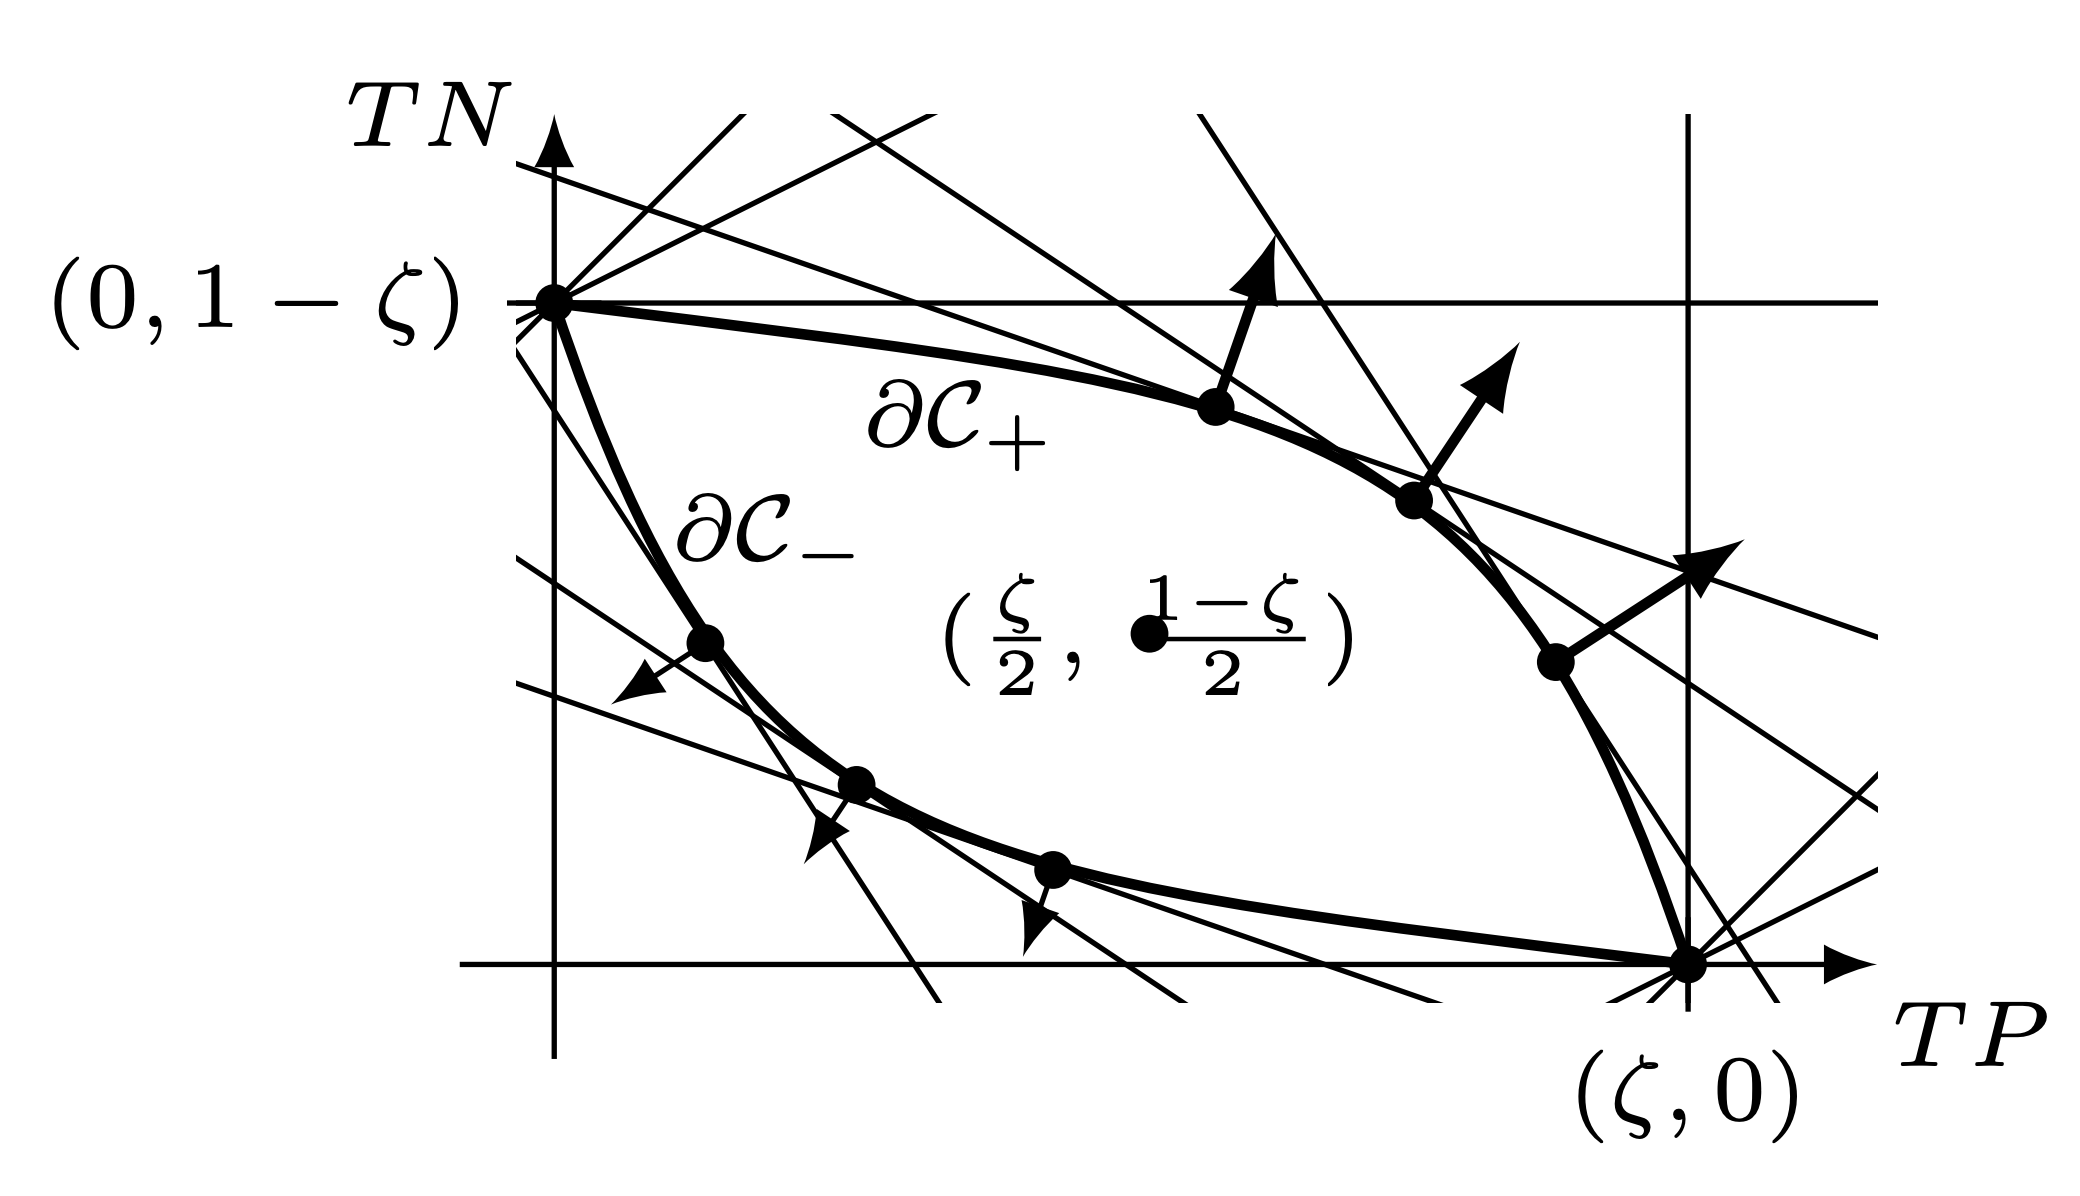
\includegraphics[width=0.5\textwidth,height=\textheight]{src/Figures/Screenshot 2023-11-13 at 6.56.44 PM.png}

}

\caption{\label{fig-c}Visual representation of \(\mathcal{C}\)}

\end{figure}%

Next, recall that an LPM is represented in terms of three parameters
(\(\phi = m_{11}TP + m_{00}TN + m_0\)). We have just seen that this LPM
and its corresponding confusion matrix correspond to a certain point on
the boundary of \(\mathcal{C}\). We first note that this point is
independent of \(m_0\). In addition, we only care about the relative
weightings of \(m_{11}\) and \(m_{00}\), not their actual values--they
are scale invariant. Therefore, we can parametrize the space of LPMs as
\(\varphi_{L P M}=\{\mathbf{m}=(\cos \theta, \sin \theta): \theta \in[0,2 \pi]\}\),
where \(\cos \theta\) corresponds to \(m_{00}\) and \(\sin \theta\)
corresponds to \(m_{11}\). And, as we already know, we can recover the
Bayes classifier given \(\mathbf{m}\), and it is unique, corresponding
to one point on the boundary of \(\mathcal{C}\), due to its convexity.
The supporting hyperplane at this point is defined as

\[\bar{\ell}_{\mathbf{m}}:=m_{11} \cdot tp+m_{00} \cdot tn=m_{11} \overline{TP}_{\mathbf{m}}+m_{00} \overline{TN}_{\mathbf{m}}\]

We note that if \(m_{00}\) and \(m_{11}\) have opposite signs, then
\(\bar{h}_m\) is the trivial classifier predicting all 1's or all 0's,
since either predicting true positives or true negatives results in
negative reward. This corresponds to a supporting hyperplane with
positive slope, so it can only be tangent at the vertices.

In addition, the boundary \(\partial \mathcal{C}\) can be split into
upper and lower boundaries
(\(\partial \mathcal{C}_{+}, \partial \mathcal{C}_{-}\)), corresponding
to \(\theta \in (0, \pi/2)\) and \(\theta \in (\pi, 3\pi/2)\)
respectively (and whether \(m_{00}, m_{11}\) are positive or negative).

\section{LPM and LFPM Metric Elicitation
Algorithms}\label{sec-orga500da0}

Now that we have established all of this background, we are ready to
present the main two results of this section. First, we introduce an
algorithm for LPM elicitation, which also forms the backbone for LFPM
elicitation.

\subsection{LPM Elicitation}\label{sec-orgb6dac4e}

For LPM elicitation, we need one more proposition.

For a metric \(\psi\) (quasiconvex and monotone increasing in TP/TN) or
\(\phi\) (quasiconcave and monotone increasing), and parametrization
\(\rho^+\)/\(\rho^-\) of upper/lower boundary, composition
\(\psi \circ \rho^-\) is quasiconvex and unimodal on {[}0, 1{]}, and
\(\phi \circ \rho^+\) is quasiconcave and unimodal on {[}0, 1{]}.

Quasiconcavity and quasiconvexity are slightly more general variations
on concavity and convexity. Their main useful property in our setting is
that they are unimodal (they have a singular extremum), so we can devise
a binary-search-style algorithm for eliciting the Bayes optimal and
inverse-optimal confusion matrices for a given setting, as well as the
corresponding \(\phi\)'s.

We first note that to maximize a quasiconcave metric, in which \(\phi\)
is monotonically increasing in \(TP\) and \(TN\), we note that the
resulting maximizer (and supporting hyperplane) will occur on the upper
boundary of \(\mathcal{C}\). We thus set our initial search range to be
\([0, \pi/2]\) and repeatedly divide it into four regions. Then, we
calculate the resulting CM on the 5 resulting boundaries of these
regions and query the oracle \(4\) times. We repeat this in each
iteration of the binary search until a maximizer is found.

In the case of quasiconcave and quasiconvex search ranges, a slightly
more sophisticated variation on typical binary search must be used. To
illustrate this, we provide the following example.

Figure 3.17: Binary search algorithm example for quasiconvex functions

Consider the two distributions in Figure \hyperref[bsearch]{3.17}. Note
that if, for both the symmetric and skewed distributions, we were to
divide the search range into two portions and compare \(A\), \(C\), and
\(E\), we would find that \(C>A\) and \(C>E\). In both of these cases,
this does not help us reduce our search range, since the true maximum
could lie on either of the two intervals (as in the second case), or at
\(C\) itself (as in the first case). Therefore, we must make comparisons
between all five points \(A, B, C, D, E\). This allows us to correctly
restrict our search range to \([B, D]\) in the first case and \([C, E]\)
in the second. These extra search requirements are due to the
quasiconcavity of the search space we are considering, in which there
exists a maximum but we need to make several comparisons at various
points throughout the search space to be able to reduce its size in each
iteration.

\textbf{input:} \(\epsilon > 0\) and oracle \(\Omega\)
\textbf{initialize:} \(\theta_a = 0, \theta_b = \frac{\pi}{2}\) set
\(\theta_c = \frac{3\theta_a+\theta_b}{4}\),
\(\theta_d = \frac{\theta_a+\theta_b}{2}\), and
\(\theta_e = \frac{\theta_a+3\theta_b}{4}\)

obtain \(h\theta_a, h\theta_c, h\theta_d, h\theta_e, h\theta_b\) using
Proposition 1

Compute \(C\theta_a, C\theta_c, C\theta_d, C\theta_e, C\theta_b\) using
(1)

Query
\(\Omega(C\theta_c, C\theta_a), \Omega(C\theta_d, C\theta_c), \Omega(C\theta_e, C\theta_d)\),
and \(\Omega(C\theta_b, C\theta_e)\)

request \(q_{i,j}\)'s label from reference impute \(q_{i,j}\)'s label
from previously labeled queries

assume the default order \(C\theta \prec C\theta' \prec C\theta''\)

assume the default order \(C\theta \prec C\theta' \prec C\theta''\)

Set \(\theta_b = \theta_d\) Set \(\theta_b = \theta_d\) Set
\(\theta_a = \theta_c\) Set \(\theta_b = \theta_e\) Set
\(\theta_a = \theta_d\) Set \(\theta_a = \theta_d\) \textbf{output:}
\(\vec{m}, C\), and \(\vec{l}\), where
\(\vec{m} = m_l(\theta_d), C = C\theta_d\), and
\(\vec{l} := (\vec{m}, (tp, tn)) = (\vec{m}, C)\)

To elicit LPMs, we run Algorithm 1 \hyperref[lpm]{{[}lpm{]}}, querying
the oracle in each iteration, and set the elicited metric \(\hat{m}\)
(which is the maximizer on \(\mathcal{C}\)) to be the slope of the
resulting hyperplane, since the metric is linear.

To find the minimum of a quasiconvex metric, we flip all instances of
\(\prec\) and \(\succ\), and use an initial search range of
\([\pi, 3\pi/2]\); we use this algorithm, which we refer to as Algorithm
2, in our elicitation of LFPMs.

Next, we provide a Python implementation of Algorithm 1.

\begin{Shaded}
\begin{Highlighting}[numbers=left,,]
\KeywordTok{def}\NormalTok{ get\_m(theta):}
    \CommentTok{"""}
\CommentTok{    Inputs: }
\CommentTok{    {-} theta: the value that parametrizes m}
\CommentTok{    Outputs:}
\CommentTok{    {-} m\_0 and m\_1 for the LPM}
\CommentTok{    """}

    \ControlFlowTok{return}\NormalTok{ (math.cos(theta), math.sin(theta))}

\KeywordTok{def}\NormalTok{ lpm\_elicitation(epsilon, oracle):}
    \CommentTok{"""}
\CommentTok{    Inputs:}
\CommentTok{    {-} epsilon: some epsilon \textgreater{} 0 representing threshold of error}
\CommentTok{    {-} oracle: some function that accepts 2 confusion matrices and}
\CommentTok{        returns true if the first is preferred and false otherwise}
\CommentTok{    Outputs:}
\CommentTok{    {-} estimate for m, which is used to compute the LPM as described above}
\CommentTok{    """}

\NormalTok{    a }\OperatorTok{=} \DecValTok{0}
\NormalTok{    b }\OperatorTok{=}\NormalTok{ math.pi}\OperatorTok{/}\DecValTok{2}
    \ControlFlowTok{while}\NormalTok{ (b }\OperatorTok{{-}}\NormalTok{ a }\OperatorTok{\textgreater{}}\NormalTok{ epsilon):}
\NormalTok{        c }\OperatorTok{=}\NormalTok{ (}\DecValTok{3} \OperatorTok{*}\NormalTok{ a }\OperatorTok{+}\NormalTok{ b) }\OperatorTok{/} \DecValTok{4}
\NormalTok{        d }\OperatorTok{=}\NormalTok{ (a }\OperatorTok{+}\NormalTok{ b) }\OperatorTok{/} \DecValTok{2}
\NormalTok{        e }\OperatorTok{=}\NormalTok{ (a }\OperatorTok{+} \DecValTok{3} \OperatorTok{*}\NormalTok{ b) }\OperatorTok{/} \DecValTok{4}

\NormalTok{        m\_a, m\_b, m\_c, m\_d, m\_e }\OperatorTok{=}\NormalTok{ (get\_m(x) }\ControlFlowTok{for}\NormalTok{ x }\KeywordTok{in}\NormalTok{ [a,b,c,d,e]) }\CommentTok{\# using definition of m}
\NormalTok{        c\_a, c\_b, c\_c, c\_d, c\_e }\OperatorTok{=}\NormalTok{ (get\_c(x) }\ControlFlowTok{for}\NormalTok{ x }\KeywordTok{in}\NormalTok{ [m\_a, m\_b, m\_c, m\_d, m\_e]) }\CommentTok{\# compute classifier from m\textquotesingle{}s then calculate confusion matrices}
        
\NormalTok{        response\_ac }\OperatorTok{=}\NormalTok{ oracle(c\_a, c\_c)}
\NormalTok{        response\_cd }\OperatorTok{=}\NormalTok{ oracle(c\_c, c\_d)}
\NormalTok{        response\_de }\OperatorTok{=}\NormalTok{ oracle(c\_d, c\_e)}
\NormalTok{        response\_eb }\OperatorTok{=}\NormalTok{ oracle(c\_e, c\_b)}

        \CommentTok{\# update ranges to keep the peak}
        \ControlFlowTok{if}\NormalTok{ response\_ac:}
\NormalTok{            b }\OperatorTok{=}\NormalTok{ d}
        \ControlFlowTok{elif}\NormalTok{ response\_cd:}
\NormalTok{            b }\OperatorTok{=}\NormalTok{ d}
        \ControlFlowTok{elif}\NormalTok{ response\_de:}
\NormalTok{            a }\OperatorTok{=}\NormalTok{ c}
\NormalTok{            b }\OperatorTok{=}\NormalTok{ e}
        \ControlFlowTok{elif}\NormalTok{ response\_eb:}
\NormalTok{            a }\OperatorTok{=}\NormalTok{ d}
        \ControlFlowTok{else}\NormalTok{:}
\NormalTok{            a }\OperatorTok{=}\NormalTok{ d}
    \ControlFlowTok{return}\NormalTok{ get\_m(d), get\_c(d)}
\end{Highlighting}
\end{Shaded}

\subsection{LFPM Elicitation}\label{sec-orga500da1}

Now, we present the next main result, which is an algorithm to elicit
linear-fractional performance metrics. For this task, we will need the
following assumption:

Let \(\phi \in \varphi_{L F P M}\). We assume
\(p_{11}, p_{00} \geq 0, p_{11} \geq q_{11}, p_{00} \geq q_{00},\)
\(p_{0}=0, q_{0}=\)
\(\left(p_{11}-q_{11}\right) \zeta+\left(p_{00}-q_{00}\right)(1-\zeta)\),
and \(p_{11}+p_{00}=1\).

These assumptions guarantee that the LFPM \(\phi\) which we are trying
to elicit is monotonically increasing in \(TP\) and \(TN\), just as in
the LPM elicitation case.

We first provide motivation and an overview of the approach for LFPM
elicitation and then present pseudocode for the algorithm.

The general idea of the algorithm is to use Algorithm 1 to obtain a
maximizer and a minimizer for the given dataset; these result in two
systems of equations involving the true LFPM \(\phi^*\) with 1 degree of
freedom. Then, we run a grid search that is independent of oracle
queries to find the point where solutions to the systems match pointwise
on the resulting confusion matrices; this occurs close to where the true
metric lies.

More formally, suppose that the true metric is
\[\phi^{*}(C)=\frac{p_{11}^{*} T P+p_{00}^{*} T N}{q_{11}^{*} T P+q_{00}^{*} T N+q_{0}^{*}}.\]
Then, let \(\bar{\tau}\) and \(\underline{\tau}\) represent the
maximizer and minimizer of \(\phi\) over \(\mathcal{C}\), respectively.
There exists a hyperplane \[\begin{aligned}
\bar{\ell}_{f}^{*}:=\left(p_{11}^{*}-\bar{\tau}^{*} q_{11}^{*}\right) t p+\left(p_{00}^{*}-\bar{\tau}^{*} q_{00}^{*}\right) t n=\bar{\tau}^{*} q_{0}^{*},
\end{aligned}\] which touches \(\mathcal{C}\) at
\(\left(\overline{T P}^{*}, \overline{T N}^{*}\right)\) on
\(\partial \mathcal{C}_{+}\).

Correspondingly, there also exists a hyperplane \[\begin{aligned}
\underline{\ell}_{f}^{*}:=\left(p_{11}^{*}-\underline{\tau}^{*} q_{11}^{*}\right) t p+\left(p_{00}^{*}-\underline{\tau}^{*} q_{00}^{*}\right) \operatorname{tn}=\underline{\tau}^{*} q_{0}^{*},
\end{aligned}\] which touches \(\mathcal{C}\) at
\(\left(\underline{TP}^{*}, \underline{T N}^{*}\right)\) on
\(\partial \mathcal{C}_{-}\). Figure~\ref{fig-minmax} illustrates this
visually on \(\mathcal{C}\).

\begin{figure}

\centering{

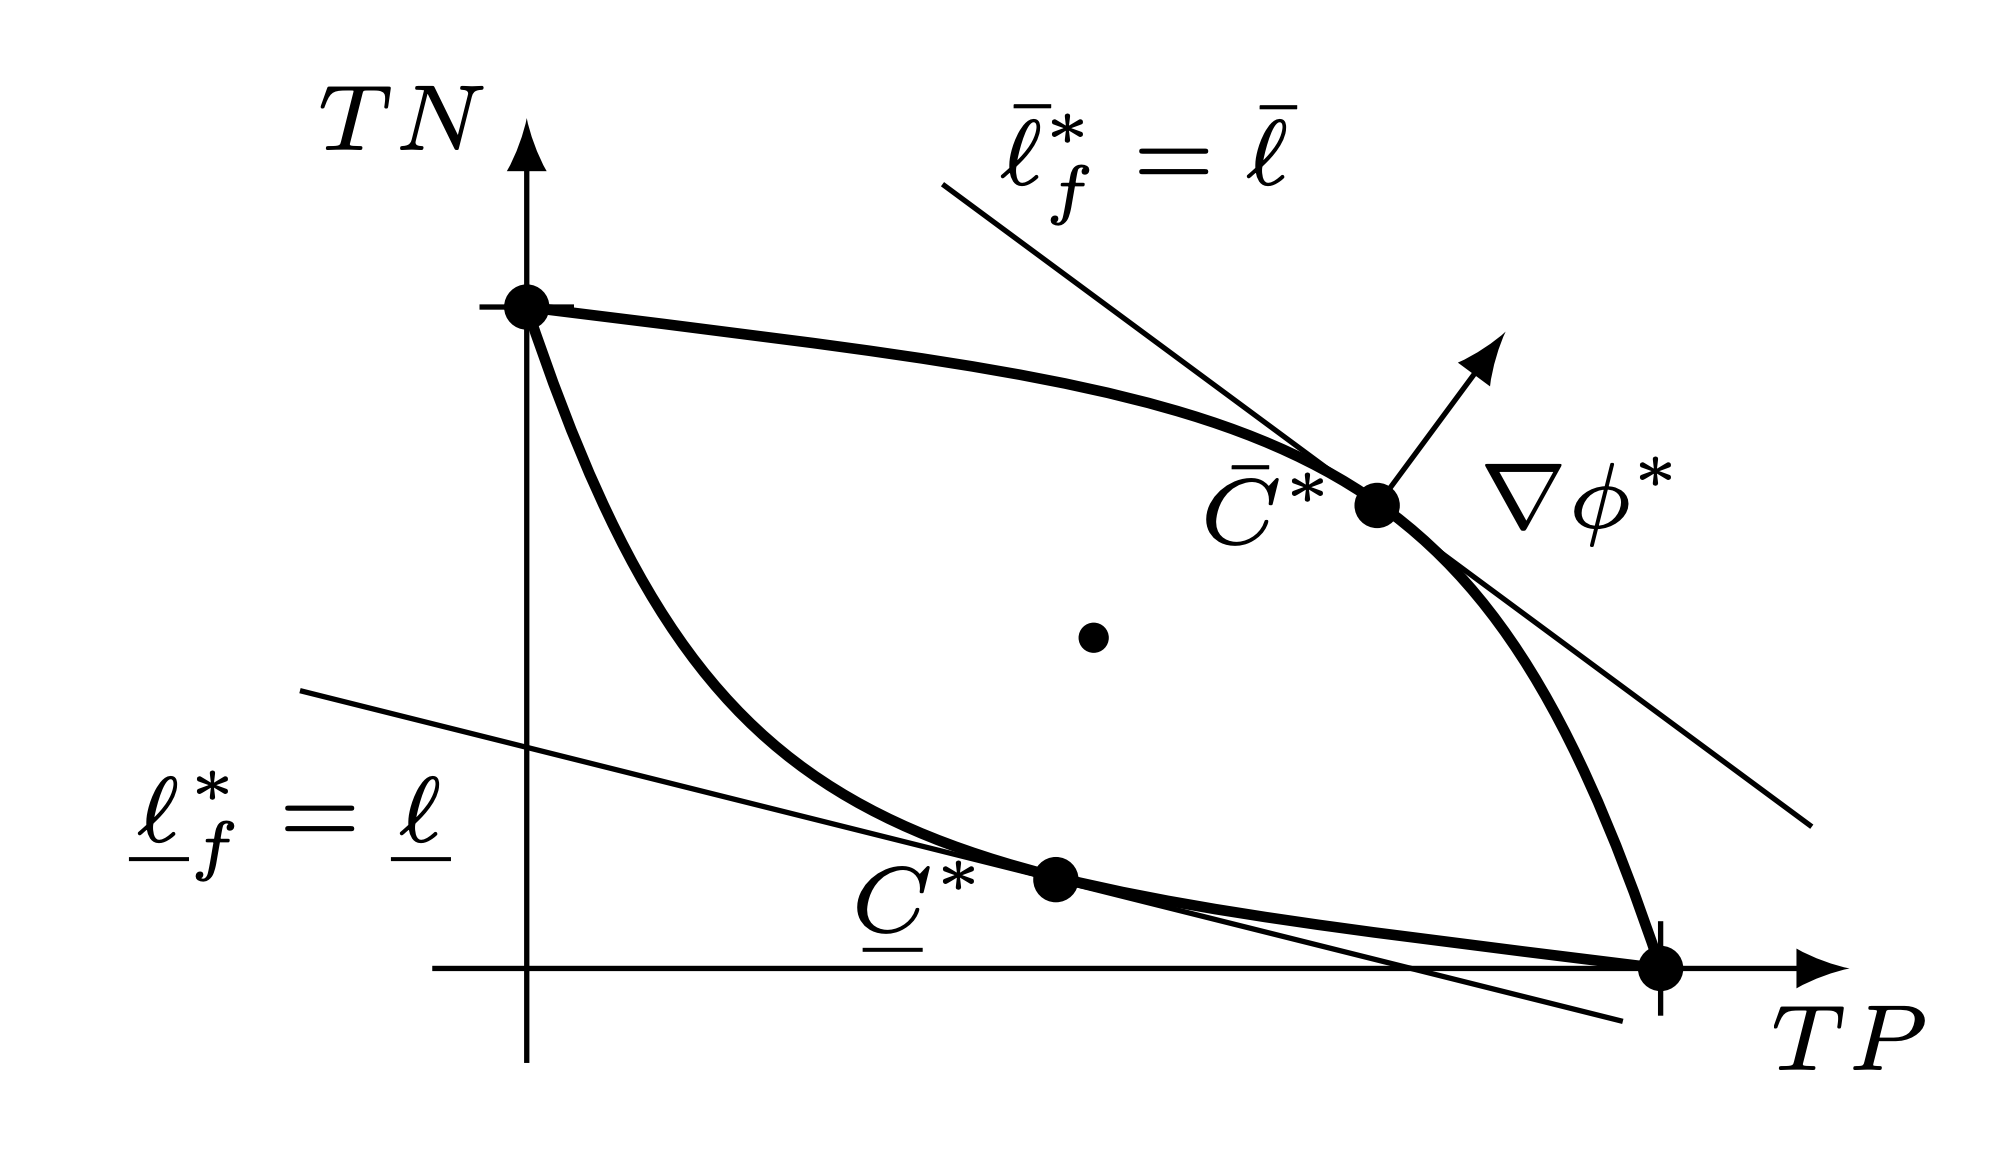
\includegraphics[width=0.5\textwidth,height=\textheight]{src/Figures/Screenshot 2023-11-13 at 6.56.52 PM.png}

}

\caption{\label{fig-minmax}Visual representation of the minimizer and
maximizer on \(\mathcal{C}\)}

\end{figure}%

While we are unable to obtain 1.1 and 1.2 directly, we can use Algorithm
1 to get a hyperplane
\[\bar{\ell}:=\bar{m}_{11} t p+\bar{m}_{00} t n= \bar{m}_{11} \overline{T P}^{*}+\bar{m}_{00} \overline{T N}^{*} = \bar{C}_{0},\]
which is equivalent to \(\bar{\ell}_{f}^{*}\) (1.1) up to a constant
multiple. From here, we can obtain the system of equations

\[p_{11}^{*}-\bar{\tau}^{*} q_{11}^{*}=\alpha \bar{m}_{11}, p_{00}^{*}-\bar{\tau}^{*} q_{00}^{*}=\alpha \bar{m}_{00}, \bar{\tau}^{*} q_{0}^{*}=\alpha \bar{C}_{0},\]
where \(\alpha > 0\) (we know it is \(\geq0\) due to our assumptions
earlier and because \(\bar{m}\) is positive, but if it is equal to \(0\)
then \(\phi^*\) would be constant. So, our resulting system of equations
is \[\begin{aligned}
    p_{11}^{\prime}-\bar{\tau}^{*} q_{11}^{\prime}=\bar{m}_{11}, p_{00}^{\prime}-\bar{\tau}^{*} q_{00}^{\prime}=\bar{m}_{00}, \bar{\tau}^{*} q_{0}^{\prime}=\bar{C}_{0}.
\end{aligned}\]

Now, similarly, we can approximate 1.2 using the algorithm we defined
for quasiconvex metrics (Algorithm 2), where we altered the search range
and comparisons. After finding the minimizer, we obtain the hyperplane
\[\underline{\ell}:=\underline{m}_{11} t p+\underline{m}_{00} t n=\underline{m}_{11} \underline{TP}^{*}+\underline{m}_{00} \underline{TN}^{*} = \underline{C}_{0},\]
which is equivalent to \(\underline{\ell}_{f}^{*}\) (1.2) up to a
constant multiple. So then, our system of equations is
\[p_{11}^{*}-\underline{\tau}^{*} q_{11}^{*}=\gamma \underline{m}_{11}, p_{00}^{*}-\underline{\tau}^{*} q_{00}^{*}=\gamma \underline{m}_{00}, \underline{\tau}^{*} q_{0}^{*}=\gamma \underline{C}_{0},\]
where \(\gamma <0\) (for a reason analogous to why we have
\(\alpha >0\)), meaning our resulting system of equations is
\[\begin{aligned}
    p_{11}^{\prime \prime}-\underline{\tau}^{*} q_{11}^{\prime \prime}=\underline{m}_{11}, p_{00}^{\prime \prime}-\underline{\tau}^{*} q_{00}^{\prime \prime}=\underline{m}_{00}, \underline{\tau}^{*} q_{0}^{\prime \prime}=\underline{C}_{0}.
\end{aligned}\]

1.3 and 1.4 form the two systems of equations mentioned in our overview
of the algorithm. Next, we demonstrate that they have only one degree of
freedom. Note that if we know \(p_{11}'\), we could solve both systems
of equations as follows: \[\begin{aligned}
    p_{00}^{\prime}  &=1-p_{11}^{\prime}, q_{0}^{\prime}=\bar{C}_{0} \frac{P^{\prime}}{Q^{\prime}}\\
    q_{11}^{\prime}  &=\left(p_{11}^{\prime}-\bar{m}_{11}\right) \frac{P^{\prime}}{Q^{\prime}} \\
    q_{00}^{\prime}&=\left(p_{00}^{\prime}-\bar{m}_{00}\right) \frac{P^{\prime}}{Q^{\prime}},
\end{aligned}\] where
\(P^{\prime}=p_{11}^{\prime} \zeta+p_{00}^{\prime}(1-\zeta)\) and
\(Q^{\prime}=P^{\prime}+\bar{C}_{0}-\)
\(\bar{m}_{11} \zeta-\bar{m}_{00}(1-\zeta).\)

Now, suppose that we were to know \(p_{11}'\). Then, we could use this
value to solve both of the systems 1.3 and 1.4, which would give us two
metrics \(\phi'\) and \(\phi''\), which come from the maximizer and
minimizer respectively. Importantly, when
\[p_{11}^{*} / p_{00}^{*}=p_{11}^{\prime} / p_{00}^{\prime}=p_{11}^{\prime \prime} / p_{00}^{\prime \prime},\]
then
\(\phi^{*}(C)=\phi^{\prime}(C) / \alpha=-\phi^{\prime \prime}(C) / \gamma\).
Essentially, when we have found a value of \(p_{11}'\) that results in
\(\phi'\), \(\phi''\) having constant ratios on all points of the
boundary of \(\mathcal{C}\), then we can obtain \(\phi^*\), since it is
obtainable from \(\phi'\) and \(\alpha\) (or, alternatively, \(\phi''\)
and \(\gamma\).)

So, we will grid search for \(p_{11}'\) on \([0,1]\). For each point in
our search, we will compute \(\phi'\) and \(\phi''\). Then, we will
generate a number of confusion matrices on the boundaries, and calculate
the ratio \(\phi'' / \phi'\) on each of them. We will select the value
of \(p_{11}'\) for which the ratio \(\phi'' / \phi'\) is the closest to
constant, and use it to compute the elicited metric \(\hat{\phi}\).

The pseudocode for LFPM elicitation is given in Figure
\hyperref[lfpm]{3.19}.

Figure 3.19: LFPM Elicitation Algorithm

Note that Algorithm 3, the grid search, is independent of oracle
queries, rendering it especially ideal for LFPM elicitation since, as a
result, our algorithm has the same algorithmic complexity as LPM
elicitation.

We provide a Python implementation below.

\begin{Shaded}
\begin{Highlighting}[numbers=left,,]
\KeywordTok{def}\NormalTok{ lfpm\_elicitation(k, delta):}
    \CommentTok{"""}
\CommentTok{    Inputs:}
\CommentTok{    {-} k: the number of confusion matrices to evaluate on}
\CommentTok{    {-} delta: the spacing for the grid search}
\CommentTok{    Outputs:}
\CommentTok{    {-} p\_11\textquotesingle{}, which will allow us to compute the elicited LFPM}
\CommentTok{    """}

\NormalTok{    sigma\_opt }\OperatorTok{=}\NormalTok{ np.inf}
\NormalTok{    p11\_opt }\OperatorTok{=} \DecValTok{0}
\NormalTok{    C }\OperatorTok{=}\NormalTok{ compute\_confusion\_matrices(k) }\CommentTok{\# generates k confusion matrices to evaluate on}

    \ControlFlowTok{for}\NormalTok{ i }\KeywordTok{in} \BuiltInTok{range}\NormalTok{(}\BuiltInTok{int}\NormalTok{(}\DecValTok{1}\OperatorTok{/}\NormalTok{delta)):}
\NormalTok{        p11 }\OperatorTok{=}\NormalTok{ i }\OperatorTok{*}\NormalTok{ delta}
\NormalTok{        phi1 }\OperatorTok{=}\NormalTok{ compute\_upper\_metric(p11) }\CommentTok{\# solves the first system of equations with p11 }
\NormalTok{        phi2 }\OperatorTok{=}\NormalTok{ compute\_lower\_metric(p11) }\CommentTok{\# solves the second system of equations with p11 }
\NormalTok{        utility\_1 }\OperatorTok{=}\NormalTok{ [phi1(c) }\ControlFlowTok{for}\NormalTok{ c }\KeywordTok{in}\NormalTok{ C] }\CommentTok{\#calculate phi for both systems of equations}
\NormalTok{        utility\_2 }\OperatorTok{=}\NormalTok{ [phi2(c) }\ControlFlowTok{for}\NormalTok{ c }\KeywordTok{in}\NormalTok{ C]}

\NormalTok{        r }\OperatorTok{=}\NormalTok{ []}
        \ControlFlowTok{for}\NormalTok{ i }\KeywordTok{in} \BuiltInTok{range}\NormalTok{(k):}
\NormalTok{            r.append(utility\_1[i] }\OperatorTok{/}\NormalTok{ utility\_2[i])}
\NormalTok{        sigma }\OperatorTok{=}\NormalTok{ np.std(r)}

        \ControlFlowTok{if}\NormalTok{(sigma }\OperatorTok{\textless{}}\NormalTok{ sigma\_opt):}
\NormalTok{            sigma\_opt }\OperatorTok{=}\NormalTok{ sigma}
\NormalTok{            p11\_opt }\OperatorTok{=}\NormalTok{ p11}
    \ControlFlowTok{return}\NormalTok{ p11\_opt}
\end{Highlighting}
\end{Shaded}

In summary, to elicit LFPMs, we utilize a special property of the LPM
minimizer and maximizer on \(\mathcal{C}\)--namely, that we can use the
corresponding supporting hyperplanes to form a system of equations that
can be used to approximate \(\phi^*\) if one parameter (\(p_{11}'\)) is
found, and that this parameter can be found using an oracle-independent
grid search.

\section{Guarantees}\label{sec-orga500da2}

Importantly, these algorithms can be shown to satisfy some important
theoretical guarantees. We provide a formal statement and intuitive
interpretation of them here, and their proofs can be found in the
appendix of the original paper.

First, we define the oracle noise \(\epsilon_{\Omega}\), which comes
from the oracle potentially flipping the comparison output on two
confusion matrices that are close enough in utility.

Given \(\epsilon, \epsilon_{\Omega} \geq 0\) and a metric \(\phi\)
satisfying our assumptions, Algorithm 1/2 finds an approximate
maximizer/minimizer and supporting hyperplane. Also, the value of
\(\phi\) at that point is within
\(O\left(\sqrt{\epsilon_{\Omega}}+\epsilon\right)\) of the optimum, and
the number of queries is \(O\left(\log \frac{1}{\epsilon}\right)\).

Let \(\mathbf{m}^{*}\) be the true performance metric. Given
\(\epsilon>0, L P M\) elicitation outputs a performance metric
\(\hat{\mathbf{m}}\), s.t.
\(\left\|\mathbf{m}^{*}-\hat{\mathbf{m}}\right\|_{\infty} \leq \sqrt{2} \epsilon+\frac{2}{k_{0}} \sqrt{2 k_{1} \epsilon_{\Omega}}\).

These two theorems ensure that Algorithms 1 and 2 find an appropriate
maximizer and minimizer in the search space, within a certain range of
accuracy that depends on oracle and sample noise, and in a certain
number of queries. Both of these statements are guaranteed by the binary
search approach.

Let \(h_{\theta}\) and \(\hat{h}_{\theta}\) be two classifiers estimated
using \(\eta\) and \(\hat{\eta}\), respectively. Further, let
\(\bar{\theta}\) be such that
\(h_{\bar{\theta}}=\arg \max _{\theta} \phi\left(h_{\theta}\right)\).
Then
\(\|C(\hat{h}_{\bar{\theta}})-C\left(h_{\bar{\theta}}\right)\|_{\infty}=O\left(\left\|\hat{\eta}_{n}-\eta\right\|_{\infty}\right)\).

This says, importantly, that the drop in elicited metric quality caused
by using a dataset of samples rather than population CMs is bounded by
the drop in performance of the decision boundary \(\eta\). These three
guarantees together ensure that oracle noise and sample noise do not
amplify drops in performance when using metric elicitation; rather,
these drops in performance are bounded by the drops that would usually
occur when using the typical machine learning paradigm of training a
decision boundary and using a pre-established metric.

\section{Summary and Further
Expansions}\label{summary-and-further-expansions}

In this chapter, we have introduced the framework of metric elicitation
for binary classification. After motivating the problem from a
psychological and theoretical perspective, we have introduced the
notions of linear performance metrics and linear-fractional performance
metrics. Next, we set up the problem of metric elicitation from a
population and sample perspective. We then made several key observations
about the space of confusion matrices which, along with the notions of
the Bayes utility and classifier, allow us to reduce the problem of
linear performance metric elicitation to a binary search algorithm over
a quasiconvex (or quasiconcave) space.

Next, we presented an algorithm to elicit linear-fractional performance
metrics that builds upon the method for eliciting linear performance
metrics. We used a key result about the dimensionality of
linear-fractional performance metrics to create a simple
oracle-independent grid search algorithm, which, in conjunction with the
linear performance metric elicitation algorithm, results in an algorithm
with the same time complexity that can be used to elicit a much broader
range of metrics. We also provided Python implementations for both of
these algorithms.

Lastly, we have described three important guarantees about the
performance of these algorithms, which makes them suited to real-world,
practical settings.

For further interesting exploration of the types of problems that can be
solved using the framework of metric elicitation, we refer the reader to
(\citeproc{ref-nips}{Hiranandani, Narasimhan, and Koyejo 2020}), which
performs metric elicitation to determine the oracle's ideal tradeoff
between the classifier's overall performance and the discrepancy between
its performance on certain protected groups.

\section{Multiclass Performance Metric
Elicitation}\label{multiclass-performance-metric-elicitation}

Although the previous chapter only described metric elicitation for
binary classification problems, the general framework can still be
applied to multiclass classification problems, as described in
``Multiclass Performance Metric Elicitation'' by Hiranandani et al.
(\citeproc{ref-NEURIPS2019_1fd09c5f}{Hiranandani et al. 2019b})

Consider the case of classifying subtypes of leukemia
(\citeproc{ref-YangNaiman+2014+477+496}{Yang and Naiman 2014}). We can
train a neural network to predict conditional probability of a certain
leukemia subtype given certain gene expressions. However, it may not be
appropriate to classify the subtype purely based on whichever one has
the highest confidence. For instance, a treatment for leukemia subtype
C1 may be perfect for cases of C1, but it may be ineffective or harmful
for certain other subtypes. Therefore, the final response from the
classifier may not be as simple as as choosing the class with the
highest conditional probability, just like how the threshold for binary
classification may not always be 50\%.

With multiclass metric elicitation, we can show confusion matrices to an
oracle (like the doctor in the leukemia example) to determine which
classifier has the best tradeoffs. In
(\citeproc{ref-NEURIPS2019_1fd09c5f}{Hiranandani et al. 2019b}), the
authors focus on eliciting linear performance metrics, which is what we
will describe in this chapter.

\section{Preliminaries}\label{preliminaries}

Most of the notation from Binary Metric Elicitation still persists, just
modified to provide categorical responses:

\begin{itemize}
\item
  \(X \in \mathcal{X}\) is the input random variable.
\item
  \(Y \in [k]\) is the output random variable, where \([k]\) is the
  index set \(\{1, 2, \dots, k\}\).
\item
  The dataset of size \(n\) is denoted by \(\{(\vec{x}, y)\}_{i=1}^n\)
  generated independently and identically from \(\mathbb{P}(X, Y)\).
\item
  \(\eta_i(\vec{x}) = \mathbb{P}(Y=i | X=\vec{x})\) gives the
  conditional probability of class \(i \in [k]\) given an observation.
\item
  \(\xi_i = \mathbb{P}(Y=i)\) is the marginal probability of class
  \(i \in [k]\).
\item
  The set of all classifiers is
  \(\mathcal{H} = \{h : \mathcal{X} \rightarrow \Delta_k\}\), where
  \(\Delta_k\) is (k-1) dimensional simplex. In this case, the outputs
  of classifiers are 1-hot vectors of size \(k\) where the only index
  with value 1 is the predicted class and all other positions have a
  value of 0.
\item
  The confusion matrix for a classifier, \(h\), is
  \(C(h, \mathbb{P}) \in \mathbb{R}^{k \times k}\), where:
  \[C_{ij}(h, \mathbb{P}) = \mathbb{P}(Y=i, h=j) \text{\qquad for } i, j \in [k]\]
\end{itemize}

Note that the confusion matrices are \(k\times k\) and store the joint
probabilities of each type of classification for each possible class.
This means that the sum of row \(i\) in the confusion matrix equals
\(\xi_i\), because this is equivalent to adding over all possible
classifications. Since we know the sums of each row, all diagonal
elements can be reconstructed from just the off-diagonal elements, so a
confusion matrix \(C(h, \mathbb{P})\) can be expressed as a vector of
off-diagonal elements,
\(\vec{c}(h, \mathbb{P}) = \textit{off-diag}(C(h, \mathbb{P}))\), and
\(\vec{c} \in \mathbb{R}^q\) where \(q := k^2 - k\). The vector
\(\vec{c}\) is called the vector of \emph{`off-diagonal confusions.'}
The space of off-diagonal confusions is
\(\mathcal{C} = \{\vec{c}(h, \mathbb{P}) : h \in \mathcal{H}\}\).

In cases where the oracle would care about the exact type of
misclassification (i.e.~misclassifying and object from class 1 as class
2), this off-diagonal confusion matrix is necessary. However, there are
many cases where the performance of a classifier is determined by just
the probability of correct prediction for each class, which just
requires the diagonal elements. In these cases, we can define the vector
of \emph{`diagonal confusions'} as
\(\vec{d}(h, \mathbb{P}) = \textit{diag}(C(h, \mathbb{P})) \in \mathbb{R}^k\).
The space of diagonal confusions is
\(\mathcal{D} = \{\vec{d}(h, \mathbb{P}) : h \in \mathcal{H}\}\).

Finally, the setup for metric elicitation is identical to the one
examined in the previous chapter. We still assume access to an oracle
that can choose between two classifiers or confusion matrices, using
notation \(\Gamma\) for comparing two classifiers and \(\Omega\) for
comparing confusion matrices, which returns 1 if the first classifier is
better and 0 otherwise. We still assume that the oracle behaves
according to some unknown performance metric, and we wish to recover
this metric up to some small error tolerance (based on a suitable norm).

The two different types of confusion vectors result in different
algorithms for metric elicitation, which we will explore in later
sections.

\section{Diagonal Linear Performance Metric
Elicitation}\label{diagonal-linear-performance-metric-elicitation}

In this section, we study metric elicitation in the case where the
performance metric is linear and we only care about diagonal confusions.

\subsection{DLPM}\label{dlpm}

A Diagonal Linear Performance Metric (DLPM) is a performance metric that
only considers the diagonal elements in the confusion matrix. The metric
is defined as \(\psi(\vec{d}) = \langle \vec{a}, \vec{d} \rangle\),
where \(\vec{a} \in \mathbb{R}^k\) such that \(||\vec{a}||_1 = 1\). It
is also called weighted accuracy
(\citeproc{ref-pmlr-v37-narasimhanb15}{Narasimhan et al. 2015}).

The family of DLPMs is denoted as \(\varphi_{DLPM}\). Since these only
consider the diagonal elements, which we want to maximize, we can focus
on only eliciting monotonically increasing DLPMs, meaning that all
elements in \(\vec{a}\) are non-negative.

\subsection{Bayes Optimal Classifiers}\label{bayes-optimal-classifiers}

The Bayes Optimal diagonal confusion given a metric \(\psi\) is
\(\bar{d} = \arg\max_{\vec{d} \in \mathcal{D}} \psi(\vec{d})\).

The Restricted Bayes Optimal (RBO) diagonal confusion is the diagonal
confusion that maximizes metric \(\psi\) given that it is only allowed
to predict classes \(k_1\) and \(k_2\). It is denoted as
\(\bar{c}_{k_1, k_2} := \arg\max_{\vec{d} \in \mathcal{D}_{k_1, k_2}} \psi(\vec{d})\).

\subsection{Geometry of Space of Diagonal Confusions
D}\label{geometry-of-space-of-diagonal-confusions-d}

Consider the trivial classifiers that only predict a single class at all
times. The diagonal confusions when only predicting class \(i\) are
\(\vec{v}_i \in \mathbb{R}^k\) with \(\xi_i\) at index \(i\) and zero
elsewhere. Note that this is the maximum possible value in index \(i\),
because this represents perfectly classifying all points that have a
true class of \(i\).

We can consider the space of diagonal confusions, visualized in
Figure~\ref{fig-diag_geom} (taken from
(\citeproc{ref-NEURIPS2019_1fd09c5f}{Hiranandani et al. 2019b})). The
space of \(\mathcal{D}\) is strictly convex, closed, and contained in
the box \([0, \xi_1] \times \dots \times [0, \xi_k]\). We also know that
the only vertices are \(\vec{v}_i\) for each \(i \in [k]^{(k-1)}\).

\begin{figure}

\centering{

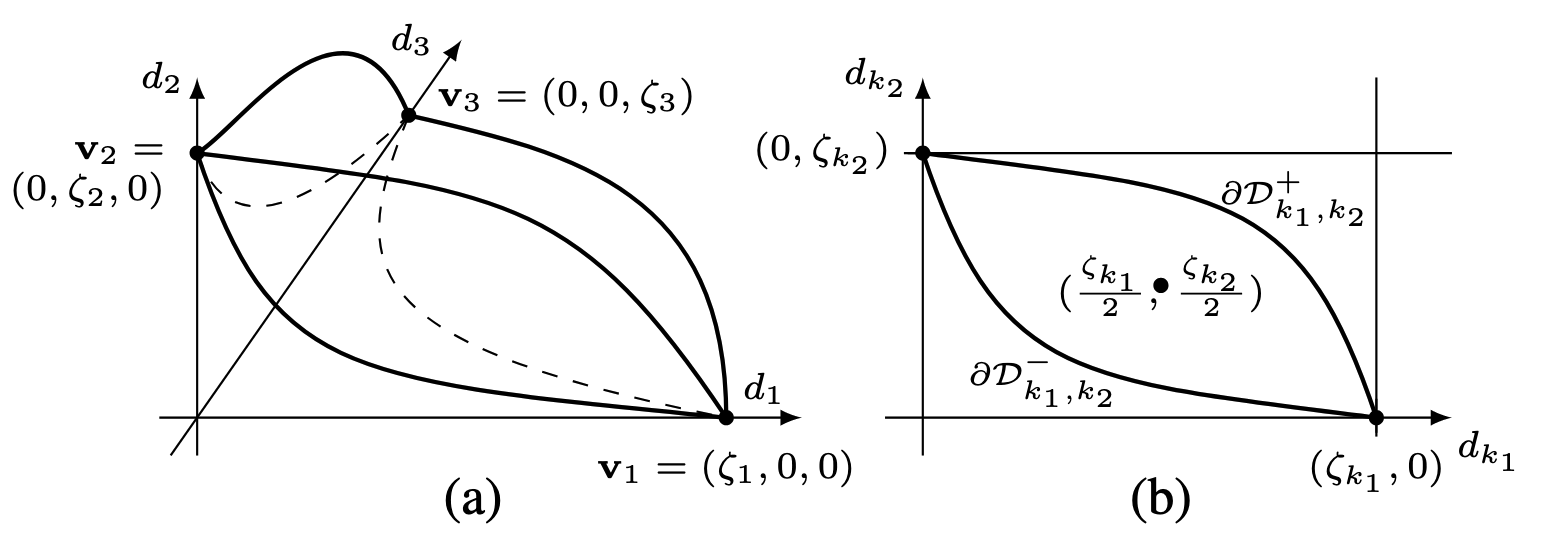
\includegraphics{src/Figures/diag_geometry.png}

}

\caption{\label{fig-diag_geom}(a) Geometry of space of diagonal
confusions for \(k=3\). This is a convex region with three flat areas
representing confusions when restricted to only two classes. (b)
Geometry of diagonal confusions when restricted to classes \(k_1\) and
\(k_2\). Notice how this is identical to the space of confusion matrices
examined in the previous chapter.}

\end{figure}%

We know that this is strictly convex under the assumption that an object
from any class can be misclassified as any other class. Mathematically,
the assumption is that
\(g_{ij}(r) = \mathbb{P} \left[\frac{\eta_i(X)}{\eta_j(X)} \geq r \right]\)
\(\forall i, j \in [k]\) are continuous and strictly decreasing for
\(r \in [0, \infty)\).

We can also define the space of binary classification confusion matrices
confined to classes \(k_1\) and \(k_2\), which is the 2-D \((k_1, k_2)\)
axis-aligned face of \(\mathcal{D}\), denoted as
\(\mathcal{D}_{k_1, k_2}\). Note that this is strictly convex, since
\(\mathcal{D}\) itself is strictly convex, and it has the same geometry
as the space of binary confusion matrices examined in the previous
chapter. Therefore, we can construct an RBO classifier for
\(\psi \in \varphi_{DLPM}\), parameterized by \(\vec{a}\), as follows:
\[\begin{aligned}
\bar{h}_{k_1, k_2}(\vec{x})= \left\{
\begin{array}{ll}
      k_1, \text{ if } a_{k_1} \eta_{k_1}(\vec{x}) \geq a_{k_2} \eta_{k_2}(\vec{x})\\
k_2, \text{ o.w.}
\end{array}
\right\}.
\end{aligned}\]

We can parameterize the upper boundary of \(\mathcal{D}_{k_1, k_2}\),
denoted as \(\partial \mathcal{D}^{+}_{k_1, k_2}\), using a single
parameter \(m \in [0, 1]\). Specifically, we can construct a DLPM by
setting \(a_{k_1} = m\), \(a_{k_2} = 1 - m\), and all others to 0. Using
equation \hyperref[rbo_eq]{{[}rbo\_eq{]}}, we can get the diagonal
confusions, so varying \(m\) parameterizes
\(\partial \mathcal{D}^{+}_{k_1, k_2}\). The parameterization is denoted
as \(\nu(m; k_1, k_2)\).

\subsection{DLPM Elicitation}\label{dlpm-elicitation}

Suppose the oracle follows a true metric, \(\psi\), that is linear and
monotone increasing across all axes. If we consider the composition
\(\psi \circ \nu(m; k_1, k_2): [0, 1] \rightarrow \mathbb{R}\), we know
it must be concave and unimodal, because \(\mathcal{D}_{k_1, k_2}\) is a
convex set. Therefore, we can find the value of \(m\) that maximizes
\(\psi \circ \nu(m; k_1, k_2)\) for any given \(k_1\) and \(k_2\) using
a binary search procedure.

Since the RBO classifier for classes \(k_1\) and \(k_2\) only rely on
the relative weights of the classes in the DLPM (see equation
\hyperref[rbo_eq]{{[}rbo\_eq{]}}), finding the value of \(m\) that
maximizes \(\psi \circ \nu(m; k_1, k_2)\) gives us the true relative
ratio between \(a_{k_1}\) and \(a_{k_2}\). Specifically, from the
definition of \(\nu\), we know that
\(\frac{a_{k_2}}{a_{k_1}} = \frac{1-m}{m}\). We can therefore simply
calculate the ratio between \(a_1\) and all other weights to reconstruct
an estimate for the true metric. A python implementation of this
algorithm is provided below.

\begin{Shaded}
\begin{Highlighting}[numbers=left,,]
\ImportTok{import}\NormalTok{ numpy }\ImportTok{as}\NormalTok{ np}

\KeywordTok{def}\NormalTok{ rbo\_dlpm(m, k1, k2, k):}
    \CommentTok{"""}
\CommentTok{    This constructs DLPM weights for the upper boundary of the}
\CommentTok{    restricted diagonal confusions, given a parameter m.}
\CommentTok{    This is equivalent to }\CharTok{\textbackslash{}n}\CommentTok{u(m; k1, k2)}
\CommentTok{    }
\CommentTok{    Inputs:}
\CommentTok{    {-} m: parameter (between 0 and 1) for the upper boundary}
\CommentTok{    {-} k1: first axis for this  face}
\CommentTok{    {-} k2: second axis for this face}
\CommentTok{    {-} k: number of classes}
\CommentTok{    Outputs:}
\CommentTok{    {-} DLPM weights for this point on the upper boundary}
\CommentTok{    """}
\NormalTok{    new\_a }\OperatorTok{=}\NormalTok{ np.zeros(k)}
\NormalTok{    new\_a[k1] }\OperatorTok{=}\NormalTok{ m}
\NormalTok{    new\_a[k2] }\OperatorTok{=} \DecValTok{1} \OperatorTok{{-}}\NormalTok{ m}
    \ControlFlowTok{return}\NormalTok{ new\_a}

\KeywordTok{def}\NormalTok{ dlpm\_elicitation(epsilon, oracle, get\_d, k):}
    \CommentTok{"""}
\CommentTok{    Inputs:}
\CommentTok{    {-} epsilon: some epsilon \textgreater{} 0 representing threshold of error}
\CommentTok{    {-} oracle: some function that accepts 2 confusion matrices and}
\CommentTok{        returns true if the first is preferred and false otherwise}
\CommentTok{    {-} get\_d: some function that accepts dlpm weights and returns }
\CommentTok{        diagonal confusions}
\CommentTok{    {-} k: number of classes}
\CommentTok{    Outputs:}
\CommentTok{    {-} estimate for true DLPM weights}
\CommentTok{    """}
\NormalTok{    a\_hat }\OperatorTok{=}\NormalTok{ np.zeros(k)}
\NormalTok{    a\_hat[}\DecValTok{0}\NormalTok{] }\OperatorTok{=} \DecValTok{1}
    \ControlFlowTok{for}\NormalTok{ i }\KeywordTok{in} \BuiltInTok{range}\NormalTok{(}\DecValTok{1}\NormalTok{, k):}
        \CommentTok{\# iterate over each axis to find appropriate ratio}
\NormalTok{        a }\OperatorTok{=} \DecValTok{0}  \CommentTok{\# lower bound of binary search}
\NormalTok{        b }\OperatorTok{=} \DecValTok{1}  \CommentTok{\# upper bound of binary search}

        \ControlFlowTok{while}\NormalTok{ (b }\OperatorTok{{-}}\NormalTok{ a }\OperatorTok{\textgreater{}}\NormalTok{ epsilon):}
\NormalTok{            c }\OperatorTok{=}\NormalTok{ (}\DecValTok{3} \OperatorTok{*}\NormalTok{ a }\OperatorTok{+}\NormalTok{ b) }\OperatorTok{/} \DecValTok{4}
\NormalTok{            d }\OperatorTok{=}\NormalTok{ (a }\OperatorTok{+}\NormalTok{ b) }\OperatorTok{/} \DecValTok{2}
\NormalTok{            e }\OperatorTok{=}\NormalTok{ (a }\OperatorTok{+} \DecValTok{3} \OperatorTok{*}\NormalTok{ b) }\OperatorTok{/} \DecValTok{4}

            \CommentTok{\# get diagonal confusions for each point}
\NormalTok{            d\_a, d\_c, d\_d, d\_e, d\_b }\OperatorTok{=}\NormalTok{ (get\_d(rbo\_dlpm(x, }\DecValTok{0}\NormalTok{, i, k)) }
                \ControlFlowTok{for}\NormalTok{ x }\KeywordTok{in}\NormalTok{ [a, c, d, e, b])}

            \CommentTok{\# query oracle for each pair}
\NormalTok{            response\_ac }\OperatorTok{=}\NormalTok{ oracle(d\_a, d\_c)}
\NormalTok{            response\_cd }\OperatorTok{=}\NormalTok{ oracle(d\_c, d\_d)}
\NormalTok{            response\_de }\OperatorTok{=}\NormalTok{ oracle(d\_d, d\_e)}
\NormalTok{            response\_eb }\OperatorTok{=}\NormalTok{ oracle(d\_e, d\_b)}

            \CommentTok{\# update ranges to keep the peak}
            \ControlFlowTok{if}\NormalTok{ response\_ac:}
\NormalTok{                b }\OperatorTok{=}\NormalTok{ d}
            \ControlFlowTok{elif}\NormalTok{ response\_cd:}
\NormalTok{                b }\OperatorTok{=}\NormalTok{ d}
            \ControlFlowTok{elif}\NormalTok{ response\_de:}
\NormalTok{                a }\OperatorTok{=}\NormalTok{ c}
\NormalTok{                b }\OperatorTok{=}\NormalTok{ e}
            \ControlFlowTok{elif}\NormalTok{ response\_eb:}
\NormalTok{                a }\OperatorTok{=}\NormalTok{ d}
            \ControlFlowTok{else}\NormalTok{:}
\NormalTok{                a }\OperatorTok{=}\NormalTok{ d}

\NormalTok{        midpt }\OperatorTok{=}\NormalTok{ (a }\OperatorTok{+}\NormalTok{ b) }\OperatorTok{/} \DecValTok{2}
\NormalTok{        a\_hat[i] }\OperatorTok{=}\NormalTok{ (}\DecValTok{1} \OperatorTok{{-}}\NormalTok{ midpt) }\OperatorTok{/}\NormalTok{ midpt}
    \ControlFlowTok{return}\NormalTok{ a\_hat }\OperatorTok{/}\NormalTok{ np.}\BuiltInTok{sum}\NormalTok{(a\_hat)}
\end{Highlighting}
\end{Shaded}

To use this algorithm for metric elicitation on a real dataset, we need
to supply the ``oracle'' and ``get\_d'' functions. The oracle function
is an interface to an expert who judges which of two confusion matrices
is better. The get\_d function will need to construct a classifier given
the DLPM weights, following the principles of the RBO classifier from
equation \hyperref[rbo_eq]{{[}rbo\_eq{]}}, and calculate the confusion
matrix from a validation set.

\subsection{DLPM Elicitation
Guarantees}\label{dlpm-elicitation-guarantees}

Using the same oracle feedback noise model from the binary metric
elicitation, we can make the following guarantees:

Given \(\epsilon, \epsilon_\Omega \geq 0\), and a 1-Lipschitz DLPM
\(\varphi^*\) parameterized by \(\vec{a}^*\). Then the output
\(\hat{a}\) of the DLPM elicitation algorithm after
\(O((k-1)\log\frac{1}{\epsilon})\) queries to the oracle satisfies
\(||\vec{a}^* - \hat{a}||_\infty \leq O(\epsilon + \sqrt{\epsilon_\Omega})\),
which is equivalent to
\(||\vec{a}^* - \hat{a}||_2 \leq O(\sqrt{k}(\epsilon + \sqrt{\epsilon_\Omega}))\).

In other words, the maximum difference between the estimate and true
value along any component (indicated by the L-infinity norm) is linearly
bounded by the sum of the epsilon specified by the algorithm and the
square root of the oracle's correctness guarantee (\(\epsilon_\Omega\)).

\section{Linear Performance Metric
Elicitation}\label{linear-performance-metric-elicitation}

In this section, we study metric elicitation in the case where
performance metric is linear and we care about the entire confusion
matrix (i.e.~the off-diagonal confusions).

A Linear Performance Metric (LPM) is a performance metric that uses the
off-diagonal confusions, which is equivalent to the whole confusion
matrix. The metric is defined as
\(\phi(\vec{c}) = \langle \vec{a}, \vec{c} \rangle\), where
\(\vec{a} \in \mathbb{R}^q\) such that \(||\vec{a}||_2 = 1\). As a
reminder, \(q = k^2 - k\), which is the number of off-diagonal elements
of the confusion matrix. The family of LPMs is denoted as
\(\varphi_{LPM}\). Since these only consider the off-diagonal elements,
which we want to minimize, we can focus on only eliciting monotonically
decreasing LPMs, meaning all elements in \(\vec{a}\) are non-positive.
The Bayes Optimal confusion given a metric \(\phi\) over a subset
\(\mathcal{S} \subseteq \mathcal{C}\) is
\(\bar{c} = \arg\max_{\vec{c} \in \mathcal{S}} \phi(\vec{c})\).

\subsection{Geometry of Space of Off-Diagonal Confusions
C}\label{geometry-of-space-of-off-diagonal-confusions-c}

Consider the trivial classifiers that only predict a single class at all
times. The off-diagonal confusions when only predicting class \(i\) are
\(\vec{u}_i \in \mathbb{R}^q\), and all \(\xi_j\) (where \(j \neq i\))
will appear in this vector, because all classes other than \(i\) will be
incorrectly predicted.

The space of off-diagonal confusions, \(\mathcal{C}\) is convex and
contained in the box
\([0, \xi_1]^{(k-1)} \times \dots \times [0, \xi_k]^{(k-1)}\). We also
know that each \(\vec{u}_i\) is a vertex. Furthermore,
\(\vec{o} = \frac{1}{k} \sum_{i=1}^k \vec{u}_i\) is always contained in
\(\mathcal{C}\) and represents the confusion matrix for the classifier
that chooses a class uniformly at random.

Notice that \(\mathcal{C}\) is not \emph{strictly} convex, unlike
\(\mathcal{D}\). However, if we make the assumption that there exists a
\(q\)-dimensional sphere \(\mathcal{S}_\lambda \subset \mathcal{C}\) of
radius \(\lambda > 0\) centered at \(\vec{o}\), we can now operate on
this convex space. Note that this sphere always exists as long as there
is some signal for non-trivial classification, so this assumption is
safe in practice. Furthermore, since we are eliciting some linear metric
with weights \(\vec{a}\), we know the optimal off-diagonal confusion
\(\bar{c}\) over \(\mathcal{S}\) is a point on its boundary
\(\bar{c} = \lambda \vec{a} + \vec{o}\).

Since we are only eliciting monotonically decreasing LPMs, we can
parameterize the lower boundary of \(\mathcal{S}_\lambda\), denoted as
\(\partial S^{-}_\lambda\), using sphere angles. Specifically, let
\(\vec{\theta}\) be a (q-1) dimensional vector of angles, with all
angles in the second quadrant (\(\theta_i \in [\pi/2, \pi]\)), except
for the primary angle, which is in the third quadrant
(\(\theta_{(q-1)} \in [\pi, 3\pi/2]\). To construct the LPM, we can set
\(a_i = \prod_{j=1}^{i-1} \sin(\theta_j) \cos(\theta_i)\) for
\(i \in [q-1]\) while \(a_q =  \prod_{j=1}^{q-1} \sin(\theta_j)\). This
parameterization ensures that all elements in \(\vec{a}\) are
non-positive and the 2-norm is 1. This parameterization is denoted as
\(\mu(\vec{\theta})\).

\subsection{LPM Elicitation}\label{lpm-elicitation}

Unlike the diagonal case, \(\mathcal{C}\) is not \emph{strictly} convex,
so the boundary may have flat regions. This means the DLPM elicitation
algorithm cannot be used in this case. Instead, we can use the query
space of the sphere \(\mathcal{S}_\lambda\) to find an optimal point,
allowing us to recover the metric.

Drawing from Derivative-Free Optimization (DFO)
(\citeproc{ref-NIPS2012_e6d8545d}{Jamieson, Nowak, and Recht 2012}), we
can perform binary search on one coordinate at a time and keep updating
cyclically. This algorithm will converge, because the metric is unimodal
(over the lower boundary of the sphere) so progress is guaranteed.

A python implementation of this algorithm is provided below.

\begin{Shaded}
\begin{Highlighting}[numbers=left,,]
\ImportTok{import}\NormalTok{ numpy }\ImportTok{as}\NormalTok{ np}

\KeywordTok{def}\NormalTok{ get\_lpm(theta):}
    \CommentTok{"""}
\CommentTok{    This constructs LPM weights for the lower boundary of the}
\CommentTok{    sphere.}
\CommentTok{    }
\CommentTok{    Inputs:}
\CommentTok{    {-} theta: parameter for the lower boundary}
\CommentTok{    Outputs:}
\CommentTok{    {-} LPM weights}
\CommentTok{    """}
\NormalTok{    new\_a }\OperatorTok{=}\NormalTok{ np.ones(theta.size }\OperatorTok{+} \DecValTok{1}\NormalTok{)}
\NormalTok{    sin\_theta }\OperatorTok{=}\NormalTok{ np.sin(theta)}
\NormalTok{    new\_a[}\DecValTok{1}\NormalTok{:] }\OperatorTok{=}\NormalTok{ sin\_theta}
\NormalTok{    new\_a[:}\OperatorTok{{-}}\DecValTok{1}\NormalTok{] }\OperatorTok{*=}\NormalTok{ np.cos(theta)}
    \ControlFlowTok{return}\NormalTok{ new\_a}

\KeywordTok{def}\NormalTok{ get\_mod\_lpm(theta, j, new\_val):}
    \CommentTok{"""}
\CommentTok{    This constructs LPM weights where index j of the parameter}
\CommentTok{    is set to new\_val}
\CommentTok{    """}
\NormalTok{    new\_theta }\OperatorTok{=}\NormalTok{ np.copy(theta)}
\NormalTok{    new\_theta[j] }\OperatorTok{=}\NormalTok{ new\_val}
    \ControlFlowTok{return}\NormalTok{ get\_lpm(new\_theta)}

\KeywordTok{def}\NormalTok{ lpm\_elicitation(epsilon, oracle, get\_c, k, T):}
    \CommentTok{"""}
\CommentTok{    Inputs:}
\CommentTok{    {-} epsilon: some epsilon \textgreater{} 0 representing threshold of error}
\CommentTok{    {-} oracle: some function that accepts 2 confusion matrices and}
\CommentTok{        returns true if the first is preferred and false otherwise}
\CommentTok{    {-} get\_c: some function that accepts lpm weights and returns }
\CommentTok{        off{-}diagonal confusions}
\CommentTok{    {-} k: number of classes}
\CommentTok{    {-} T: maximum number of iterations}
\CommentTok{    Outputs:}
\CommentTok{    {-} estimate for true DLPM weights}
\CommentTok{    """}
\NormalTok{    q }\OperatorTok{=}\NormalTok{ k }\OperatorTok{*}\NormalTok{ k }\OperatorTok{{-}}\NormalTok{ k}
\NormalTok{    theta }\OperatorTok{=}\NormalTok{ np.random.rand(q}\OperatorTok{{-}}\DecValTok{1}\NormalTok{)}
\NormalTok{    theta[:}\OperatorTok{{-}}\DecValTok{1}\NormalTok{] }\OperatorTok{=}\NormalTok{ (}\DecValTok{1} \OperatorTok{+}\NormalTok{ theta[:}\OperatorTok{{-}}\DecValTok{1}\NormalTok{]) }\OperatorTok{*}\NormalTok{ np.pi}\OperatorTok{/}\DecValTok{2}  \CommentTok{\# initialize params to [pi/2, pi]}
\NormalTok{    theta[:}\OperatorTok{{-}}\DecValTok{1}\NormalTok{] }\OperatorTok{=}\NormalTok{ (}\DecValTok{2} \OperatorTok{+}\NormalTok{ theta[:}\OperatorTok{{-}}\DecValTok{1}\NormalTok{]) }\OperatorTok{*}\NormalTok{ np.pi}\OperatorTok{/}\DecValTok{2}  \CommentTok{\# last param in [pi, 3pi/2]}

    \ControlFlowTok{for}\NormalTok{ t }\KeywordTok{in} \BuiltInTok{range}\NormalTok{(T):}
\NormalTok{        j }\OperatorTok{=}\NormalTok{ t }\OperatorTok{\%}\NormalTok{ (q}\OperatorTok{{-}}\DecValTok{1}\NormalTok{)  }\CommentTok{\# current coordinate to optimize}

        \CommentTok{\# initialize range of binary search}
        \ControlFlowTok{if}\NormalTok{ j }\OperatorTok{==}\NormalTok{ q}\OperatorTok{{-}}\DecValTok{2}\NormalTok{:}
\NormalTok{            a }\OperatorTok{=}\NormalTok{ np.pi}
\NormalTok{            b }\OperatorTok{=} \DecValTok{3} \OperatorTok{*}\NormalTok{ np.pi }\OperatorTok{/} \DecValTok{2}
        \ControlFlowTok{else}\NormalTok{:}
\NormalTok{            a }\OperatorTok{=}\NormalTok{ np.pi }\OperatorTok{/} \DecValTok{2}
\NormalTok{            b }\OperatorTok{=}\NormalTok{ np.pi}
        
        \ControlFlowTok{while}\NormalTok{ (b }\OperatorTok{{-}}\NormalTok{ a }\OperatorTok{\textgreater{}}\NormalTok{ epsilon):}
\NormalTok{            c }\OperatorTok{=}\NormalTok{ (}\DecValTok{3} \OperatorTok{*}\NormalTok{ a }\OperatorTok{+}\NormalTok{ b) }\OperatorTok{/} \DecValTok{4}
\NormalTok{            d }\OperatorTok{=}\NormalTok{ (a }\OperatorTok{+}\NormalTok{ b) }\OperatorTok{/} \DecValTok{2}
\NormalTok{            e }\OperatorTok{=}\NormalTok{ (a }\OperatorTok{+} \DecValTok{3} \OperatorTok{*}\NormalTok{ b) }\OperatorTok{/} \DecValTok{4}

            \CommentTok{\# get confusions for each point}
\NormalTok{            c\_a, c\_c, c\_d, c\_e, c\_b }\OperatorTok{=}\NormalTok{ (get\_c(get\_mod\_lpm(theta, j, x)) }
                \ControlFlowTok{for}\NormalTok{ x }\KeywordTok{in}\NormalTok{ [a, c, d, e, b])}

            \CommentTok{\# query oracle for each pair}
\NormalTok{            response\_ac }\OperatorTok{=}\NormalTok{ oracle(c\_a, c\_c)}
\NormalTok{            response\_cd }\OperatorTok{=}\NormalTok{ oracle(c\_c, c\_d)}
\NormalTok{            response\_de }\OperatorTok{=}\NormalTok{ oracle(c\_d, c\_e)}
\NormalTok{            response\_eb }\OperatorTok{=}\NormalTok{ oracle(c\_e, c\_b)}

            \CommentTok{\# update ranges to keep the peak}
            \ControlFlowTok{if}\NormalTok{ response\_ac:}
\NormalTok{                b }\OperatorTok{=}\NormalTok{ d}
            \ControlFlowTok{elif}\NormalTok{ response\_cd:}
\NormalTok{                b }\OperatorTok{=}\NormalTok{ d}
            \ControlFlowTok{elif}\NormalTok{ response\_de:}
\NormalTok{                a }\OperatorTok{=}\NormalTok{ c}
\NormalTok{                b }\OperatorTok{=}\NormalTok{ e}
            \ControlFlowTok{elif}\NormalTok{ response\_eb:}
\NormalTok{                a }\OperatorTok{=}\NormalTok{ d}
            \ControlFlowTok{else}\NormalTok{:}
\NormalTok{                a }\OperatorTok{=}\NormalTok{ d}

\NormalTok{        midpt }\OperatorTok{=}\NormalTok{ (a }\OperatorTok{+}\NormalTok{ b) }\OperatorTok{/} \DecValTok{2}
\NormalTok{        theta[j] }\OperatorTok{=}\NormalTok{ midpt}
    \ControlFlowTok{return}\NormalTok{ get\_lpm(theta)}
\end{Highlighting}
\end{Shaded}

Similar to the DLPM case, we need to supply the ``oracle'' and
``get\_c'' functions. The oracle function is an interface to an expert
who judges which of two confusion matrices is better. The get\_c
function will need to construct a classifier given the LPM weights,
following the fact that \(\bar{c} = \lambda \vec{a} + \vec{o}\), and
calculate the confusion matrix from a validation set. Using the same
oracle feedback noise model from the binary metric elicitation, we can
make the following guarantees:

Given \(\epsilon, \epsilon_\Omega \geq 0\), and a 1-Lipschitz LPM
\(\phi^*\) parameterized by \(\vec{a}^*\). Suppose
\(\lambda \gg \epsilon_\Omega\), then the output \(\hat{a}\) of the LPM
elicitation algorithm after
\(O(z_1 \log(z_2/(q\epsilon^2))(q-1) log(\frac{\pi}{2\epsilon}))\)
queries to the oracle satisfies
\(||a^* - \hat{a}||_2 \leq O(\sqrt{q}(\epsilon + \sqrt{\epsilon_\Omega/\lambda}))\),
where \(z_1\) and \(z_2\) are constants independent of \(\epsilon\) and
\(q\).

\section{Summary}\label{summary}

In this chapter, we explore multiclass performance metric elicitation,
extending metric elicitation beyond binary classification. In practice,
if weighted accuracy is all that is needed to determine if one
classifier is better than another, the DLPM elicitation algorithm is
preferred for its lower query complexity. However, if the type of
misclassification is important, like in the leukemia example at the
start of this chapter, the LPM elicitation algorithm enables more
flexibility.

\section{Linear Reward Estimation}\label{linear-reward-estimation}

How exactly do robots learn human preferences from just the pairwise
comparisons, if they need to learn how to act in the environment itself?
The comparisons in turn help robots learn the reward function of the
human, which allows them to further take actions in real settings.

\subsection{Geometry of Pairwise
Comparisons}\label{geometry-of-pairwise-comparisons}

Let's say there are two trajectories \(\xi_A\) and \(\xi_B\) that might
be taken as the next course of action in any context, like choosing the
next turn, or choosing the next chatGPT response. The robot is offering
both to a human for comparison. To answer which of them is better, the
human would ask themselves if \(R(\xi_A)\) or \(R(\xi_B)\) is bigger,
with \(R(\xi) = w * \phi(\xi)\) being the reward function. In this
equation \(w\) and \(\phi(\xi)\) are vectors of weights and features of
the trajectory, so alternatively, we can express this as:

\(R(\xi) = \begin{bmatrix} w_1 \\ w_2 \\ ... \\ w_N \end{bmatrix} \cdot \begin{bmatrix} \phi_1(\xi) \\ \phi_2(\xi) \\ ... \\ \phi_N(\xi) \end{bmatrix}\)

If one says that they preferred \(\xi_2\) less than \(\xi_1\) then it
means
\(\xi_2 < \xi_1 \implies R(\xi_2) < R(\xi_1) \implies w * \phi(\xi_2) < w * \phi(\xi_1) \implies 0 < w * (\phi(\xi_1) - \phi(\xi_2)) \implies 0 < w * \Phi\).
Alternatively, if one preferred \(\xi_2\) more than \(\xi_1\), the signs
would be flipped, resulting in \(0 > w * \Phi\). The two results can be
represented in the N-dimensional space, where when it is split by the
decision boundary, it creates half-spaces indicating preferences for
each of the sides. For example in Figure~\ref{fig-2dcomp} we can see how
a query between two objects can split the plain into two halves,
indicating preference towards one of the objects. Such an image can be
extended into bigger dimensions, where a line would become a separating
hyperplane like in Figure~\ref{fig-2dcomp}.

\begin{figure}

\begin{minipage}{0.50\linewidth}

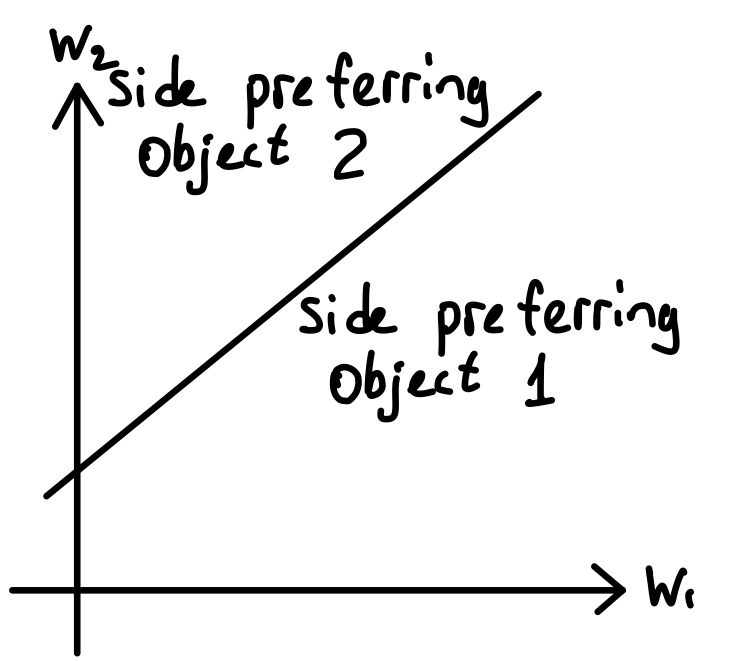
\includegraphics[width=0.4\textwidth,height=\textheight]{src/Figures/2D-comp.jpg}

\subcaption{\label{}A single query for a comparison between the two
objects splits 2D space into two halves, each of which prefers one of
the objects based on feature weights \(w_1\) and \(w_2\).}
\end{minipage}%
%
\begin{minipage}{0.50\linewidth}

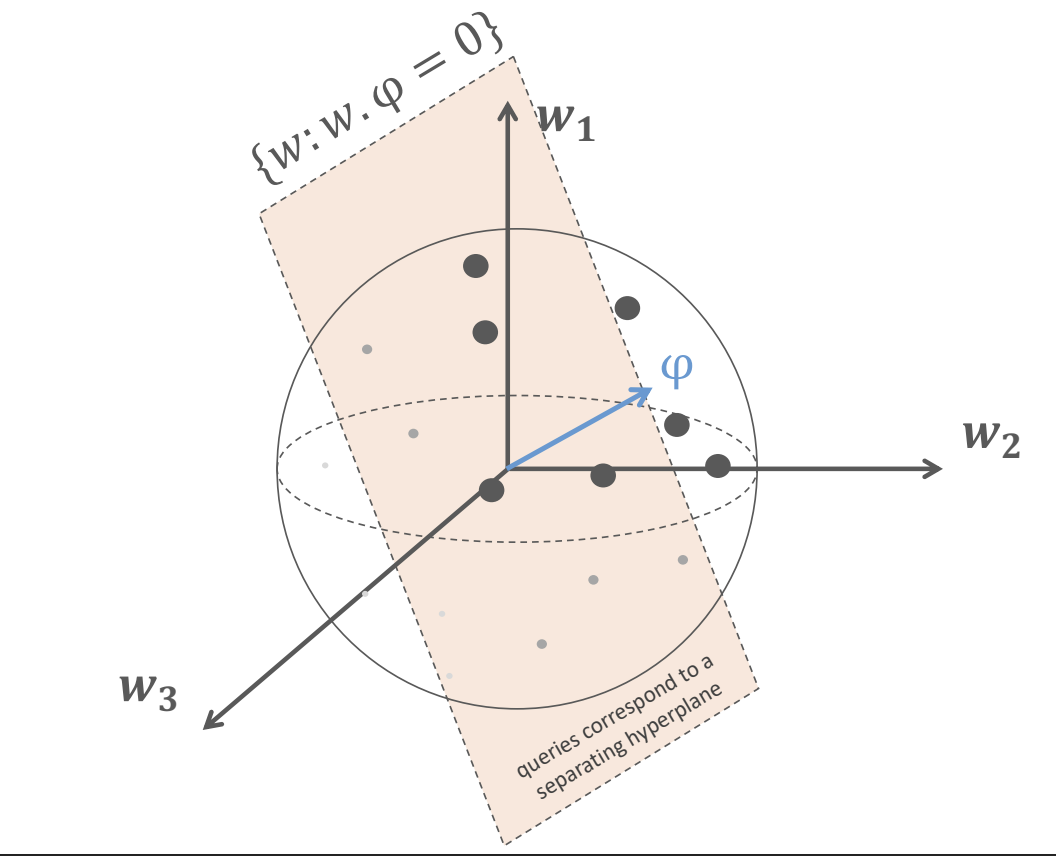
\includegraphics[width=0.4\textwidth,height=\textheight]{src/Figures/3D-comp.png}

\subcaption{\label{}Extension into 3D space}
\end{minipage}%

\caption{\label{fig-2dcomp}Comparison in 2D and 3D}

\end{figure}%

If one is to truly believe the answers of one person, they would remove
everything from the other side of the hyperplane that does not agree
with the received human preference. But since humans are noisy, that
approach is not optimal, thus most applications up-weight the indicated
side of the plane to emphasize that points on that side are better, and
down-weight the other side as they do not agree with the provided
comparison.

How should someone choose which queries to conduct, otherwise, what is
the most informative query sequence? After completing one query, the
next query should be orthogonal to the previous one so that the
potential space consistent with the preferences decreases in half. The
intuition behind that is the potential space has all of the reward
functions that agree with the provided answers, so to find a specific
reward function for a human, decreasing the space narrows down the
possible options. For example, orthogonal query to the query in
Figure~\ref{fig-2dcomp} is shown in Figure~\ref{fig-2dspace}. The
original query created the blue space, and a new one created a red
space, resulting in a purple intersection of the two which is still
consistent with both of the queries's results. The image shows that the
purple portion is exactly half of the blue portion.

\begin{figure}

\centering{

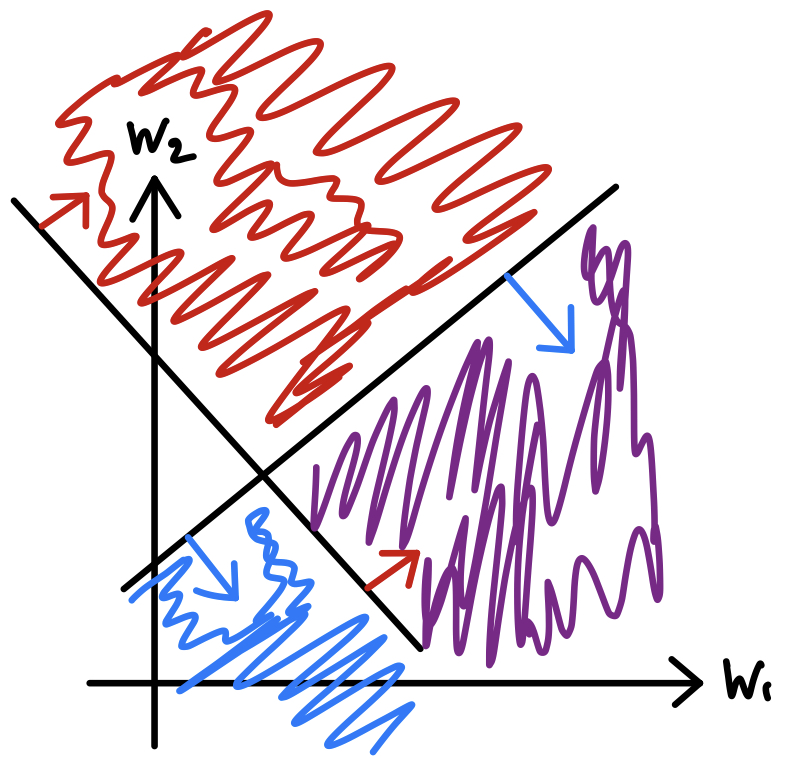
\includegraphics[width=0.4\textwidth,height=\textheight]{src/Figures/2D-space.jpg}

}

\caption{\label{fig-2dspace}Creating further comparisons limits the
space that agrees with answers to all of them. The blue area
demonstrates a preference for object 1 over object 2. The red area
demonstrates a preference for object 3 over object 4. Combination
(purple area) shows the space that is consistent with both of those
preferences.}

\end{figure}%

Mathematically, from (\citeproc{ref-pmlr-v87-biyik18a}{Biyik and Sadigh
2018}) this can be expressed as set \(F\) of potential queries \(\phi\),
where
\(F = \{\phi: \phi = \Phi(\xi_A) - \Phi(\xi_B), \xi_A, \xi_B \in \Xi\}\)
(defining that a query is the difference between the features of two
trajectories). Using that, the authors define a human update function
\(f_{\phi}(w) = \min(1, \exp(I^T\phi))\) that accounts for how much of
the space will still be consistent with the preferences. Finally, for a
specific query, they define the minimum volume removed as
\(\min\{\mathbb{E}[1 - f_{\phi}(w)], \mathbb{E}[1 - f_{-\phi}(w)]\}\)
(expected size of the two sides of the remaining space after it is split
by a query - purple area in Figure~\ref{fig-2dspace}), and the final
goal is to maximize that amount over all possible queries since it is
optimal to get rid of as much space as possible to narrow down the
options for the reward function:
\(\max_{\phi} \min\{ \mathbb{E}[1 - f_{\phi}(w)], \mathbb{E}[1 - f_{-\phi}(w)]\}\).
Effectively this is finding such \(\phi\) that maximizes the information
one can get by asking the next comparison query. While this approach
uses minimum volume removed, there can be other metrics inside the
\(\max\) function. Some applications like movie recommendations do not
require extra constraints, however in robotics one might want to add
more constraints that satisfy certain rules, so that the resulting query
follows the dynamics of the physical world.

\subsection{Driving Simulator Example}\label{driving-simulator-example}

The first real example of learning reward functions from pairwise
comparisons is a 2D driving simulator from
(\citeproc{ref-pmlr-v87-biyik18a}{Biyik and Sadigh 2018}). In
Figure~\ref{fig-car_direct} you can see the setting of a 3-lane road
with the orange car being controlled by the computer.

\begin{figure}

\centering{

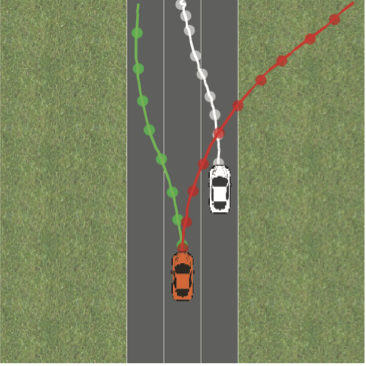
\includegraphics[width=0.4\textwidth,height=\textheight]{src/Figures/car_dir.png}

}

\caption{\label{fig-car_direct}The choices presented to a human for
feedback are represented by green and red trajectories. White trajectory
demonstrates the lane change of another vehicle in the space.
(\citeproc{ref-pmlr-v87-biyik18a}{Biyik and Sadigh 2018})}

\end{figure}%

The queries conducted for this problem are two different trajectories
presented to the human, and they are asked to evaluate which one of them
is better. For the features that contribute to the reward function, it
is important to consider that robots might not find some of the
information as informative for the learning process as a human would.
For this example, the underlying features included the distance between
lane boundaries, distance to other cars, and the heading and speed of
the controlled car. The weights toward the last feature were weighted
the highest according to the authors, since it takes a lot of effort for
the car to change or correct its direction.

At the start of the learning process, the car had no direction learned
and was moving all over the road. In the middle of learning after 30
queries, the simulator learned to follow the direction of the road and
go straight but still experienced collisions. After 70 queries, the
simulator learned to avoid collisions, as well as keep the car within
the lane without swerving.

\subsection{Active Learning for Pairwise
Comparisons}\label{active-learning-for-pairwise-comparisons}

We have discussed that pairwise comparisons should be selected to
maximize the minimum volume of remaining options removed. The question
that can come out of the driving example is does it really matter to
follow that goal or does random choice of queries performs as well? It
turns out that indeed most active learning algorithms (purposefully
selecting queries) over time converge with the performance of the random
query selection, so in long term the performance is similar. However,
what is different is that active learning achieves better performance
earlier, which in time-sensitive tasks can be a critical factor.

One example of such a setting can be exoskeletons for humans as part of
the rehabilitation after surgery (\citeproc{ref-Li_2021}{Li et al.
2021}). Different people have significantly different walking patterns
as well as rehabilitation requirements, so the exoskeleton needs to
adapt to the human as soon as possible for a more successful
rehabilitation. Figure Figure~\ref{fig-robotics} demonstrates the
difference in the time needed between the two approaches. In general, in
robotics, the time differences that might seem small to a human might be
detrimental to the final performance.

\begin{figure}

\centering{

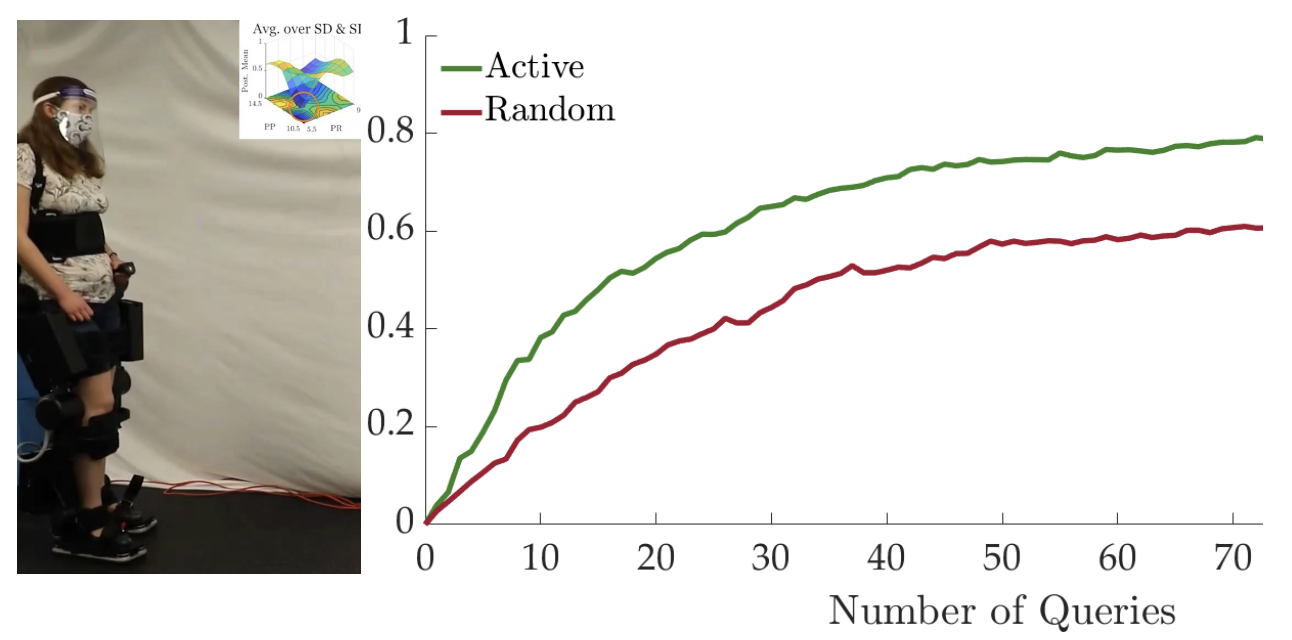
\includegraphics[width=0.6\textwidth,height=\textheight]{src/Figures/robo_graph.png}

}

\caption{\label{fig-robotics}Performance of active learning and random
query selection algorithms in the task of exoskeleton learning with
human preferences. (\citeproc{ref-Li_2021}{Li et al. 2021})}

\end{figure}%

\subsection{Multi-Modal Reward Functions for Pairwise
Comparisons}\label{multi-modal-reward-functions-for-pairwise-comparisons}

What if one is working with multiple people and their responses to the
queries for comparisons? It will be impossible to recover the different
personalities based on the answers, and it might be necessary to conduct
a full ranking before it is clear which responses belonged to which
person, but the underlying theory for the number of comparisons is
non-trivial. For that, the researchers
(\citeproc{ref-myers2021learning}{Myers et al. 2021}) have used
multi-modal models for reward function learning, which allows to account
for different types of valid behaviours and trajectories that can come
from different humans.

\begin{figure}

\centering{

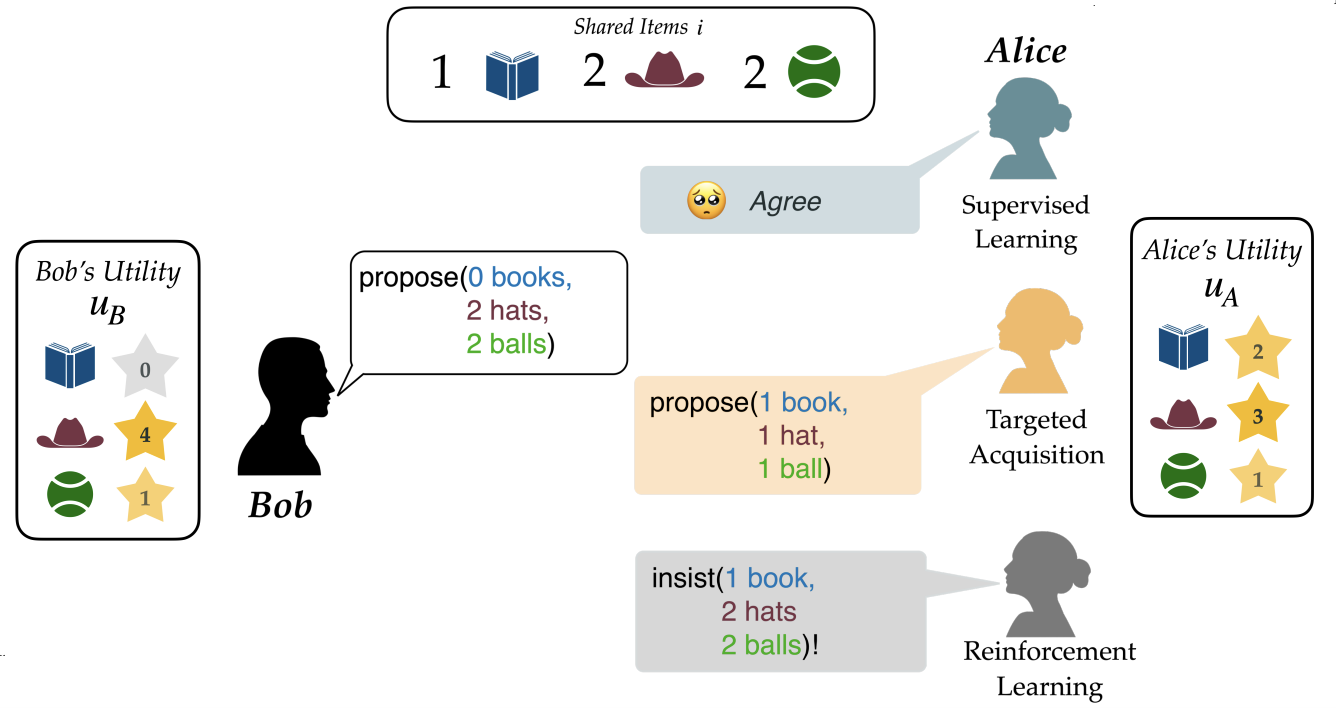
\includegraphics[width=0.8\textwidth,height=\textheight]{src/Figures/negotiation.png}

}

\caption{\label{fig-negotiation}The negotiation setting with two people
and three shared items. Each person has a desired number of items
indicated in their utility box. Alice is the controlled agent that has
many different response options that are illustrated by the approaches
different models might take. (\citeproc{ref-kwon2021targeted}{Kwon et
al. 2021})}

\end{figure}%

An example setting for such type of problem is negotiations
(\citeproc{ref-kwon2021targeted}{Kwon et al. 2021}). Let's say there are
some shared items and two people with different utilities and desires
for items, where each person only knows their utility. In a specific
case of Figure~\ref{fig-negotiation}, Bob as a proposing agent and Alice
as a controlled agent who has many different ways of responding to Bob's
proposals. Different methods can be used to design Alice as an AI agent.
The first idea is reinforcement learning, where multiple rounds of
negotiations are done, the model simulates game theory and sees how Bob
reacts. Authors of this setting (\citeproc{ref-kwon2021targeted}{Kwon et
al. 2021}) show that over time the model learns to ask for the same
thing over and over again, as Alice is not trained to be human-like or
negotiable, and just tries to maximize Alice's utility. The second
approach is supervised learning, where the model can be trained on some
dataset, learning the history of negotiations. This results in Alice
being very agreeable, which demonstrates two polar results of the two
approaches, and it would be ideal to find a middle ground and combine
both of them. The authors proposed the Targeted acquisition approach,
which is based on active learning ideas. The model asks diverse
questions at different cases and stages of negotiations like humans,
determining which questions are more valuable to be asked throughout
learning. Such an approach ended up in more fair and optimal results
than supervised or reinforcement learning
(\citeproc{ref-kwon2021targeted}{Kwon et al. 2021}).

In conclusion, pairwise comparisons show to be a great way of learning
linear reward functions, but at times present challenges or
incapabilities that can be further improved with additional
incorporations of approaches like Active Learning. That improves many
applications in terms of time spent getting to the result in case of
exoskeleton adjustments, as well as getting to a middle ground between
polar behaviors in applications like negotiations.

\section{Guiding Human Demonstrations in
Robotics}\label{guiding-human-demonstrations-in-robotics}

A strong approach to learning policies for robotic manipulation is
imitation learning, the technique of learning behaviors from human
demonstrations. In particular, interactive imitation learning allows a
group of humans to contribute their own demonstrations for a task,
allowing for scalable learning. However, not all groups of demonstrators
are equally helpful for interactive imitation learning.

The ideal set of demonstrations for imitation learning would follow a
single, optimal method for performing the task, which a robot could
learn to mimic. Conversely, \emph{multimodality}, the presence of
multiple optimal methods in the demonstration set, is challenging for
imitation learning since it has to learn from contradicting information
for how to accomplish a task.

A common reason for multimodality is the fact that different people
often subconsciously choose different paths for execution, as
illustrated in Figure~\ref{fig-multimodalexecution}.

\begin{figure}

\centering{

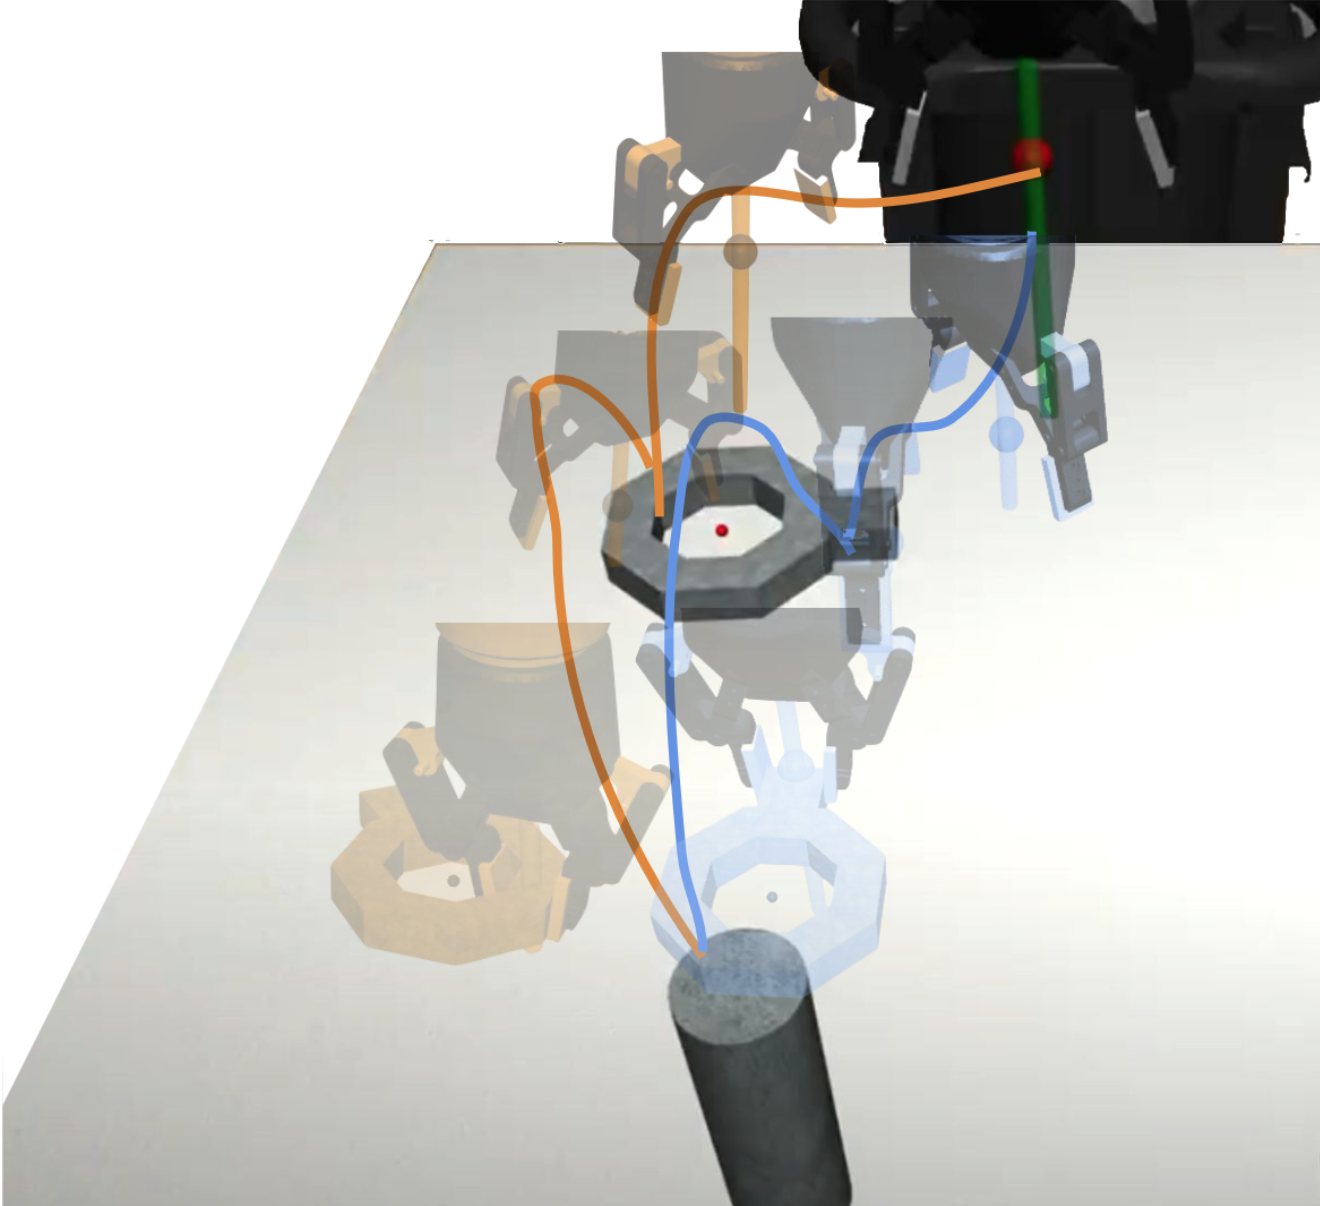
\includegraphics[width=0.5\textwidth,height=\textheight]{src/Figures/multimodal_peg.png}

}

\caption{\label{fig-multimodalexecution}Examples of two different ways
to insert a nut onto a round peg. The orange demonstration picks up the
nut from the hole while the blue demonstration picks up the nut from the
side (\citeproc{ref-gandhi2022eliciting}{Gandhi et al. 2022})}

\end{figure}%

Gandhi et al. (\citeproc{ref-gandhi2022eliciting}{Gandhi et al. 2022})
identifies whether demonstrations are compatible with one another and
offer an active elicitation interface to guide humans to provide better
demonstrations in interactive imitation learning. Their key motivation
is to allow multiple users to contribute demonstrations over the course
of data collection by guiding users towards compatible demonstrations.

To identify whether a demonstration is ``compatible'' with a base policy
trained with prior demonstrations, the researchers measure the
\emph{likelihood} of demonstrated actions under the base policy, and the
\emph{novelty} of the visited states. Intuitively, low likelihood and
low novelty demonstrations should be excluded since they represent
conflicting modes of behavior on states that the robot can already
handle, and are therefore incompatible. This concept of compatibility is
used for filtering a new set of demonstrations and actively eliciting
compatible demonstrations.

In the following subsections, we describe the process of estimating
compatibility and active elicitation in more detal.

\subsection{Estimating Compatiblity}\label{estimating-compatiblity}

We want to define a compatibility measure \(\mathcal{M}\), that
estimates the performance of policy \(\pi_{base}\) that is retrained on
a union of \(\mathcal{D}_{base}\), the known base dataset, and
\(\mathcal{D}_{new}\), the newly collected dataset. To define this
compatibility measure in a way that is easy to compute, we can use two
interpretable metrics: likelihood and novelty.

The likelihood of actions \(a_{new}\) in \(\mathcal{D}_{new}\) is
measured as the negative mean squared error between actions predicted by
the base policy and this proposed action:

\[\begin{aligned}
    likelihood(s_{new}, a_{new}) = -\mathbb{E}[|| \pi_{base}(s_{new}) - a_{new} ||^2_2].
\end{aligned}\]

The novelty of the state \(s_{new}\) in \(\mathcal{D}_{new}\) is the
standard deviation in the predicted actions under base policy:

\[\begin{aligned}
    novelty(s_{new}) = \mathrm{Var}[\pi_{base}(s_{new})].
\end{aligned}\]

We can plot likelihood and novelty on a 2D plane, as shown in
Figure~\ref{fig-likelihood_novelty}, and identify thresholds on
likelihood and novelty, denoted as \(\lambda\) and \(\eta\)
respectively. Intuitively, demonstrations with low likelihood in low
novelty states should be excluded, because this indicates that there is
a conflict between the base behavior and the new demonstration due to
multimodality. Note that in high novelty states, the likelihood should
be disregarded because the base policy does not have a concrete idea for
how to handle these states anyways so more data is needed.

\begin{figure}

\centering{

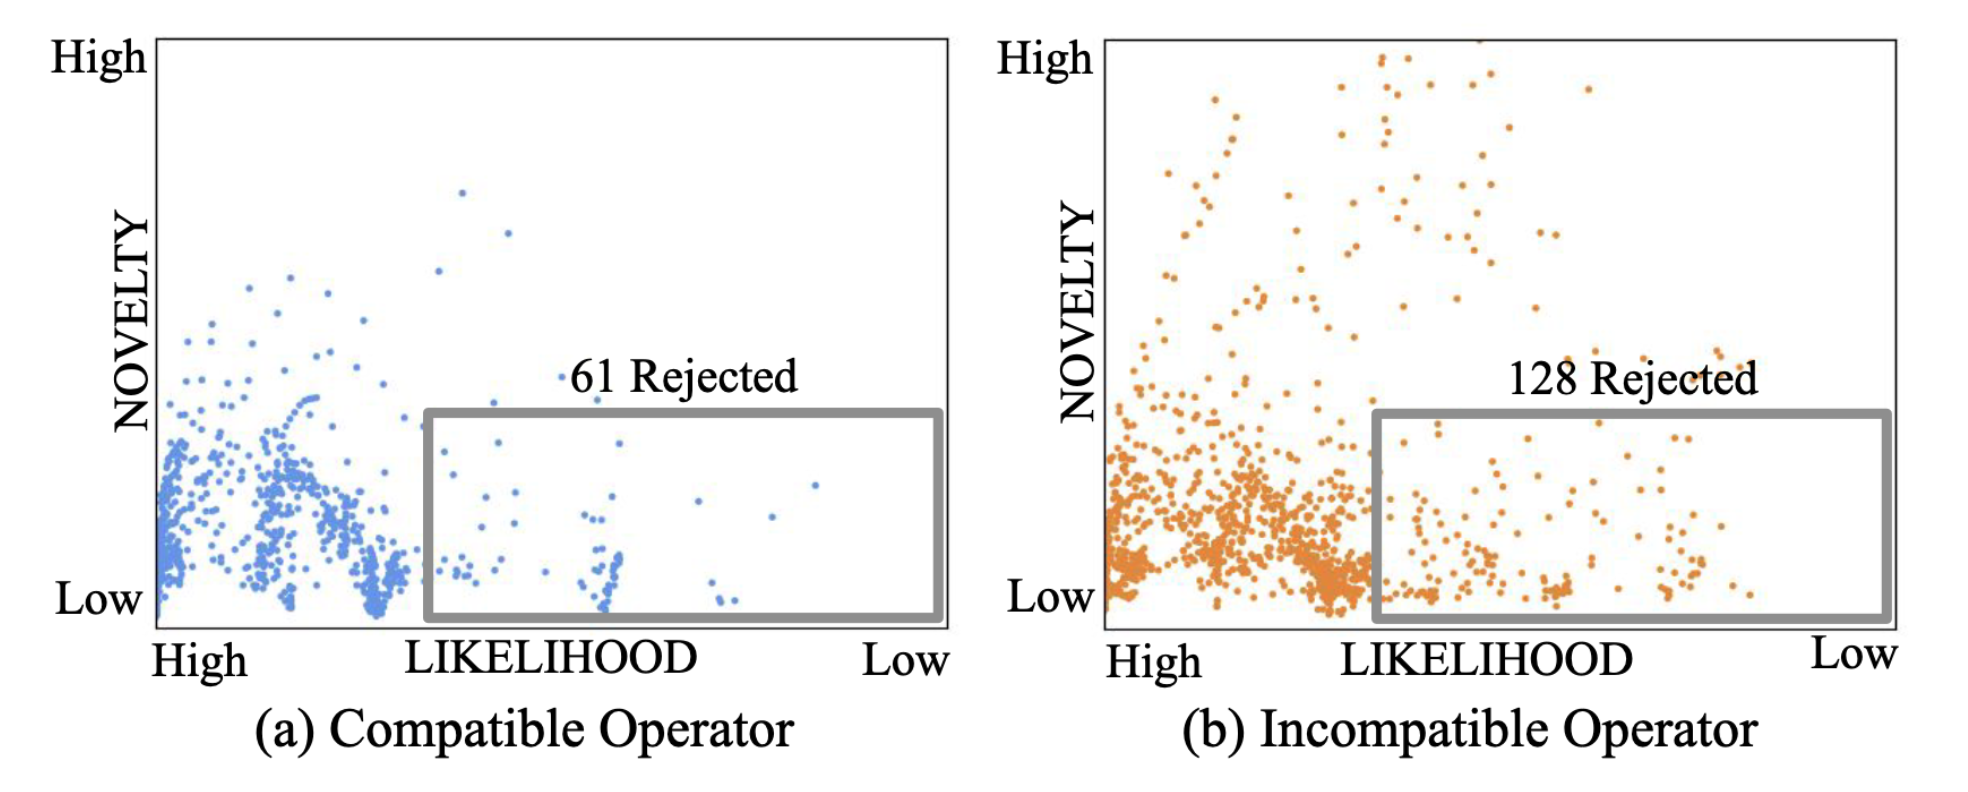
\includegraphics[width=0.8\textwidth,height=\textheight]{src/Figures/likelihood_novelty.png}

}

\caption{\label{fig-likelihood_novelty}Examples of plots of likelihood
and novelty for compatible and incompatible operators
(\citeproc{ref-gandhi2022eliciting}{Gandhi et al. 2022})}

\end{figure}%

The final compatibility metric, parameterized by the likelihood and
novelty thresholds \(\lambda\) and \(\eta\), is
\(\mathcal{M}(\mathcal{D}_{base}, (s_{new}, a_{new})) \in [0, 1]\),
defined as:

\[\begin{aligned}
    \mathcal{M} = \begin{cases} 
        1 - \min(\frac{\mathbb{E}[|| \pi_{base}(s_{new}) - a_{new} ||^2_2]}{\lambda}, 1) & \text{ if } \textsc{novelty}(s_{new}) < \eta \\
        1 & \text{ otherwise }
       \end{cases}.
\end{aligned}\]

Note that \(\lambda\) and \(\eta\) need to be specified by hand. This is
accomplished by assuming the ability to collect \emph{a priori
incompatible} demonstrations to identify reasonable thresholds that
remove the most datapoints in the incompatible demonstrations while
keeping the most datapoints in the compatible demonstrations.

\subsection{Case Studies with Fixed
Sets}\label{case-studies-with-fixed-sets}

The researchers evaluate the utility of the compatibility metric on
three tasks: placing a square nut on a square peg, placing a round nut
on a round peg, and opening a drawer and placing a hammer inside. For
each task, they train a base policy using a ``proficient'' operator's
demonstration while sampling trajectories from other operators for the
new set.

The naive baseline is to use all datapoints while the
\(\mathcal{M}\)-Filtered demonstrations use the compatibility metric to
filter out incompatible demonstrations. The results are presented in
Table~\ref{tbl-m_filter_table}. As you can see, M-filtering results in
equal or greater performance despite using less data than the naive
baseline, demonstrating the effectiveness of compatibility-based
filtering.

\begin{longtable}[]{@{}lclclcl@{}}
\caption{Success rates (mean/std across 3 training runs) for policies
trained on \(\mathcal{D}_{new}\) by using all the data (Naive) or
filtering by compatibility (\(\mathcal{M}\)-Filtered)
(\citeproc{ref-gandhi2022eliciting}{Gandhi et al.
2022})}\label{tbl-m_filter_table}\tabularnewline
\toprule\noalign{}
\endfirsthead
\endhead
\bottomrule\noalign{}
\endlastfoot
& \textbf{Square Nut} & & \textbf{Round Nut} & & \textbf{Hammer
Placement} & \\
\textbf{Operator} & Naive & \(\mathcal{M}\)-Filtered & Naive &
\(\mathcal{M}\)-Filtered & Naive & \(\mathcal{M}\)-Filtered \\
Base Operator & 38.7 (2.1) & - & 13.3 (2.3) & - & 24.7 (6.1) & - \\
Operator 1 & 54.3 (1.5) & 61.0 (4.4) & 26.7 (11.7) & 32.0 (12.2) & 38.0
(2.0) & 39.7 (4.6) \\
Operator 2 & 40.3 (5.1) & 42.0 (2.0) & 22.0 (7.2) & 26.7 (5.0) & 33.3
(3.1) & 32.7 (6.4) \\
Operator 3 & 37.3 (2.1) & 42.7 (0.6) & 17.3 (4.6) & 18.0 (13.9) & 8.0
(0.0) & 12.0 (0.0) \\
Operator 4 & 27.3 (3.5) & 37.3 (2.1) & 7.3 (4.6) & 13.3 (1.2) & 4.0
(0.0) & 4.0 (0.0) \\
\end{longtable}

\begin{figure}

\centering{

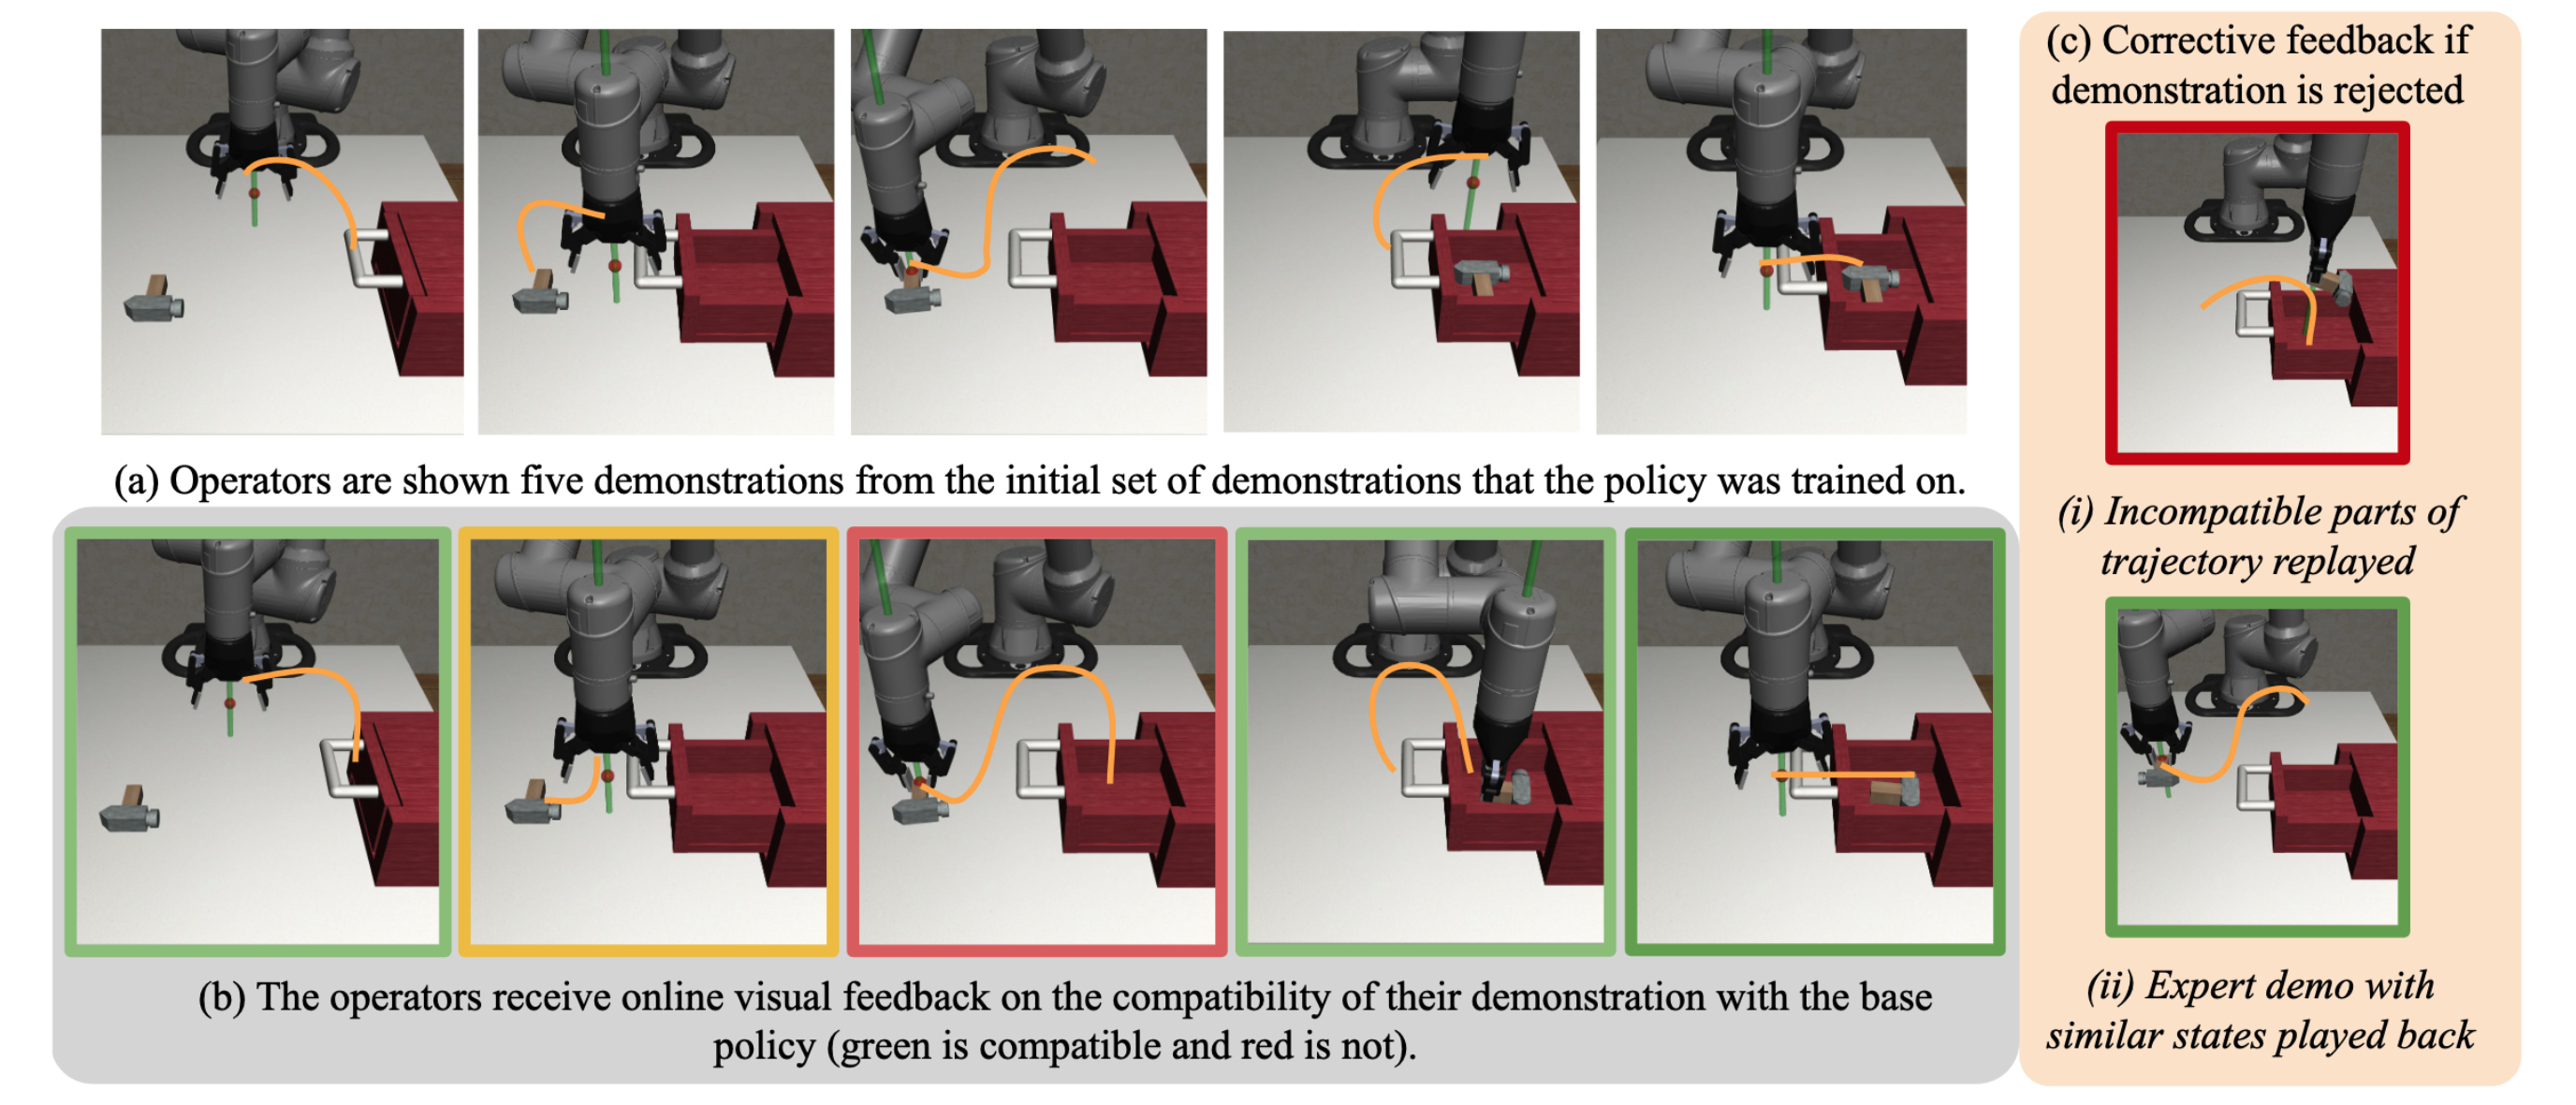
\includegraphics[width=0.8\textwidth,height=\textheight]{src/Figures/active_elicitation.png}

}

\caption{\label{fig-active_elicitation}The phases of the active
elicitation interface: (a) initial prompting, (b) demonstrations with
live feedback, and (c) corrective feedback
(\citeproc{ref-gandhi2022eliciting}{Gandhi et al. 2022})}

\end{figure}%

\subsection{Actively Eliciting Compatible
Demonstrations}\label{actively-eliciting-compatible-demonstrations}

In the previous section, we assume access to a dataset that has already
been collected, and we see how filtering out incompatible demonstrations
helps improve performance. However, when collecting a new dataset, it
would be better to ensure that operators collect compatible
demonstrations from the start, allowing us to retain as much data as
possible for training.

To actively elicit compatible demonstrations, the researchers set up a
pipeline for live feedback and examples. At the start, operators are
given a task specification and some episodes to practice using the
robot. Then, the active elicitation process begins, as shown in
Figure~\ref{fig-active_elicitation}. Each operator is shown some
rollouts of the base policy to understand the style of the base
operator. Next, the operator provides a demonstration similar to the
ones they were shown. As they record their demonstrations, the interface
provides online feedback, with green indicating compatible actions and
red indicating incompatible actions. If the number of incompatible
state-action pairs (ones where \(\mathcal{M}\) is zero) exceeds 5\% of
the demonstration length, the demonstration is rejected. However, to
provide corrective feedback, the interface shows the areas of the
demonstration with the highest average incompatibility and also provides
an expert demo that shows what should actually be done. Demonstrators
can use this feedback to provide more compatible demonstrations moving
forward.

This process helps improve the demonstration quality in both simulation
and real experiments, as show in
Table~\ref{tbl-active_elicitation_results}. Specifically, on the real
results, active elicitation outperformed the base policy by 25\% and
naive data collection by 55\%. Overall, active elicitation is a powerful
tool to ensure that data collected for imitation learning improves the
quality of the learned policy.

\begin{longtable}[]{@{}lcccc@{}}
\caption{Success rates (mean/std across users) for policies trained on
\(\mathcal{D}_{new}\) by using all the data (Naive), filtering by
compatibility (\(\mathcal{M}\)-Filtered), or using informed
demonstration collection (\citeproc{ref-gandhi2022eliciting}{Gandhi et
al. 2022})}\label{tbl-active_elicitation_results}\tabularnewline
\toprule\noalign{}
\textbf{Task} & \textbf{Base} & \textbf{Naive} & \textbf{Naive +
Filtered} & \textbf{Informed} \\
\midrule\noalign{}
\endfirsthead
\toprule\noalign{}
\textbf{Task} & \textbf{Base} & \textbf{Naive} & \textbf{Naive +
Filtered} & \textbf{Informed} \\
\midrule\noalign{}
\endhead
\bottomrule\noalign{}
\endlastfoot
\textbf{Round Nut} & 13.3 (2.3) & 9.6 (4.6) & 9.7 (4.2) & 15.7 (6.0) \\
\textbf{Hammer Placement} & 24.7 (6.1) & 20.8 (15.7) & 22.0 (15.5) &
31.8 (16.3) \\
\textbf{\(\left[ \textup{Real} \right]\) Food Plating} & 60.0 & 30.0
(17.3) & - & 85.0 (9.6) \\
\end{longtable}

\subsection{Limitations and Future Work for Active
Elicitation}\label{limitations-and-future-work-for-active-elicitation}

A fundamental limitation of eliciting compatible demonstrations is the
fact that the ``base'' demonstrator is considered the ground truth. When
the base demonstrator specifies a preference, all other demonstrators
must abide by it, even if they have strong preferences against it. For
instance, when pouring milk and cereal into a bowl, different people
have different preferences for what is the correct order, but active
elicitation forces all demonstrators to follow the initial preference of
the base operator. The researchers hope that future work can enable
users to override the default demonstration set and follow a base
behavior that better aligns with their preferences. This could enable
multiple modes of behavior to be collected in data while only following
a user's specified preference instead of attempting to collapse all
modes into a single policy.

Looking forward, active elicitation provides a foundation for allowing
robots to query humans about the type of data needed, enabling more
efficient data collection through transparency.

\section{Conclusion}\label{conclusion-1}

In summary, this chapter has explored the complexities and innovations
in interactive learning as applied to large models within robotics. It
begins by investigating pairwise comparisons and their role in
efficiently learning linear reward functions from large datasets,
overcoming limitations in supervised learning. When combined with active
learning techniques, these comparisons supply timely, targeted, and
context-appropriate feedback, enhancing performance in time-critical
applications like exoskeleton adjustments during rehabilitation.

We then shift to imitation learning or inverse reward learning from
demonstrations, emphasizing the difficulties introduced by multimodal
demonstration sets. active elicitation approaches to compile compatible
demonstrations, streamlining the learning process by guiding users to
provide more valuable, steady examples are incredibly promising,
however, to tackling this issue. This method shows promise in refining
the interactive imitation learning data collection pipeline, enabling
more capable and effective robotic training.

Additionally, the chapter examines the integration of foundation models
into robotics, highlighting the transformative innovations of R3M and
Voltron. R3M's pre-training on diverse human activities dramatically
improves robotic manipulation with minimal supervision. Meanwhile,
Voltron builds on these capabilities by incorporating language-driven
representation learning for remarkably adaptable and nuanced robotic
task performance. These models represent significant leaps in robotics
while opening new frontiers for future research and applications.

\section{Truthful Preference Elicitation with
Adversary}\label{truthful-preference-elicitation-with-adversary}

In our study of social choice models in Chapter
\hyperref[2human-decision-making-choice-models]{{[}2model{]}}, we study
how axiomatic properties are implemented to prevent strategic
manipulation of a population. This brings us onto the field of
\textbf{mechanism design}. At its core, mechanism design is the science
of making rules. The intent in this field is to design systems so that
the strategic behaviour of individuals leads to desirable outcomes. Just
thinking about services on the Internet -- file sharing, reputation
systems, web search, web advertising, email, Internet auctions,
congestion control -- all have to be set up so that an individual's
selfish behavior leads to better outcomes for the entire community. A
more specific example of this is the phenomenon of ``bid-sniping'' that
was present on eBay in the early 2000s. When people could bid on E-bay,
the rule was that the highest bidder by the end of some specified time
period would get the item. As a result, people would just wait until the
very last minute to bid in order to not raise the price of the item too
early. On the other hand, when Amazon still allowed bidding, they had a
rule that any time a bid was placed it would extend the time of the bid
by ten minutes. This simple difference had drastic effects on bidding
prices over time. Mechanism design develops the theoretical framework
for learning social choices and eliciting truthful preference.

We will cover frameworks that model several scenarios that mechanism
design is usefully applied to: recommendation systems (where users will
selfishly try to stick to their preferences while a planner encourages
exploration); auctions (where bidders will try to maximise their reward
compared to others); and peer grading (where truthful reporting is not
necessarily an incentive for students).

\subsection{Auction Theory}\label{auction-theory}

\subsubsection*{Single-Item Auctions}\label{single-item-auctions}
\addcontentsline{toc}{subsubsection}{Single-Item Auctions}

The first problem within auction theory we will consider is the
\emph{single-item auction}. The premise of this problem is that there is
a single item to sell, \(n\) bidders (with unknown private valuations of
the item \(v_1\), ..., \(v_n\)). The bidder's individual objective is to
maximize utility: the value \(v_i\) of the item subtracted by the price
paid for the item. The auction procedure is standard in the sense that
bids are solicited and the highest bid will win the auction. While the
objective of the individual bidder is clear, there could be a plethora
of different objectives for the auction as a whole. One option could be
to maximize social surplus, meaning the goal is to maximize the value of
the winner. Another objective could be to maximize seller profit which
is the payment of the winner. For simplicity, we can focus on the first
objective where the goal is to maximize social surplus. If we want to
maximize social surplus it turns out that a great way to do this is the
``second-price auction''.

\paragraph*{Maximizing Social Surplus}\label{maximizing-social-surplus}
\addcontentsline{toc}{paragraph}{Maximizing Social Surplus}

In the second-price auction, we will operate under slightly different
conditions. In the second-price auction we 1) solicit sealed bids, 2)
have the winner be the highest bidder, and 3) charger winner the
second-highest bid price. As an example, if the solicited bids are
\(b = (2, 6, 4, 1)\) the winner will be that who bid \(6\), but will pay
a price of \(4\). From here, we can do some equilibrium analysis to try
and learn what the optimal bidding strategy is for each bidder. Let the
amount bidder \(i\) bids to be \(b_i\), so we have bids
\(b_1, b_2, ..., b_n\). How much should bidder \(i\) bid? To analyze
this, let us define \(t_i = max_{j \neq i} b_j\) which represents the
max of the bids that is not from bidder \(i\). There are now two cases
to consider: if \(b_i\) \textgreater{} \(t_i\) and if \(b_i\)
\textless{} \(t_i\). In the first case the bidder \(i\) wins, and if the
bidder bid \(b_i = v_i\), they are guaranteed to have a positive return
on bid. In the other case, they lose the bid and the net loss is 0
because they don't have to pay. From this we can conclude that bidder
\(i\)'s dominant strategy is to just bid \(b_i = v_i\). Rigorously
proving this is a little bit trickier, but it was shown from Vickrey in
1961 {[}cite{]} that truthful bidding is the dominant strategy in
second-price auctions. A corollary of this is that we are maximizing
social surplus since bids are values and the winner is the bidder with
highest valuation.

\paragraph*{Maximize Seller Profit}\label{maximize-seller-profit}
\addcontentsline{toc}{paragraph}{Maximize Seller Profit}

If we want to look at things from the perspective of a seller trying to
maximize their profit we need to treat the bidder's bids as uniform
random variables. Consider the example scenario where we have two
bidders each bidding uniformly between 0 and 1. What is the seller's
expected profit? (in this case profit and revenue for the seller are the
same because we assume the seller throws away the item if it doesn't
sell/has no valuation for it).

From there the question now becomes, can we get more expected profit
from the seller's perspective? It turns out there is a design where we
can add a reserve price of \(r\) to the second-price auction. The way
this works is we can 1) Insert seller-bid at \(r\), 2) solicit bids, 3)
pick the highest bidder, and 3) charge the 2nd-highest bid. In effect,
this is just the second-price auction but with a bid from the seller as
well, at a price of \(r\). A lemma, that we won't prove here, is that
the second-price auction with reserve price \(r\) still has a dominant
strategy of just being truthful.

Let's now consider what the profit of a second-price auction would be
with two bidders that uniformly bid between 0 and 1 -- but this time we
have a reserve price of \(1/2\). To calculate the expected profit we
break down the situation into 3 cases:

\begin{itemize}
\item
  Case 1:
  \(1/2 > v_1 > v_2 \rightarrow 1/4 \text{ probability} \rightarrow  E[\text{profit}] = 0\)
\item
  Case 2:
  \(v_1 > v_2 > 1/2 \rightarrow 1/4 \text{probability} \rightarrow E[v2 | case 2] = 2/3\)
\item
  Case 3:
  \(v_1 > 1/2 > v_2 \rightarrow 1/2 \text{ probability} \rightarrow 1/2\)
\end{itemize}

Why is \(E[v2 | case 2] = 2/3\)? If \(v_1\) and \(v_2\) are greater than
\(1/2\), they are evenly spread across the interval, meaning the
expectation will be 1/2 + 1/6 = 2/3. Adding up all these cases we get
\(E[profit] = 5/12\). It turns out that second-price auctions with
reserve actually maximize profit in general (for symmetric bidders)!

In the previous section we conclude that second-price auctions with
reserve maximize profit for the seller. In order to prove this, we now
move to the more general topic of asking how should a monopolist divide
good across separate markets. We can make the assumption that the demand
model is a concave revenue \(R(q)\) in quantity \(q\). Under this
assumption, we can just divide supply into \(q = q_a + q_b\) such that
\(R'_a(q_a) = R'_b(q_b)\). The idea from here is a theorem from Myerson
in 1981 that states an optimal action maximizes "marginal revenue".
Consider an example where we have two bidders bidding a uniform value
between 0 and 1. Our revenue curve can now be derived from the offering
price \(V(q) = 1 - q\) like so: \(R(q) = qV(q) = q - q^2\). Taking the
derivative gives us the marginal revenue \(R'(q) = 1-2q\). This means
two things: 1) we want to sell to bidder \(i\) with the highest
\(R'(q_i)\) and 2) we want to sell to bidder \(i\) with value at least
\(1/2\) (if we want a positive \(R'(q_i)\). But this is just a
second-price auction with reserve \(1/2\)! This means that for symmetric
bidders, a second price with reserve is the optimal auction.

\paragraph*{What good are auctions?}\label{what-good-are-auctions}
\addcontentsline{toc}{paragraph}{What good are auctions?}

An interesting topic to discuss is what benefits auctions bring to the
table as opposed to just standard pricing. Online auctions used to be a
lot more popular in the early 2000s and have been completely replaced by
standard online pricing, even on sites like e-bay. While auctions are
slower and have added inherent complexities, they are actually optimal
on paper. Standard pricing on the other is non-optimal; although it is
fast and simpler for buyers. There is actually a way to quantify this:
for pricing \(k\) units, the loss is at most \(1 / \sqrt{2\pi k}\) of
optimal profit.

Let's consider applications in duopoly platform design. We know that the
optimal auction is second-price with reserve, but what happens when we
introduce competition between two auction platforms? Some important
details related to the revenue of a second-price auction is that a
second-price auction with no reserve and n bidders leads to larger
revenue having an optimal reserve and n - 1 bidders
(\citeproc{ref-bulow-klemperer1996}{Bulow and Klemperer 1996}).
Additionally, with an entry cost, no reserve is the optimal strategy for
maximizing revenue (\citeproc{ref-mcafee-87}{McAfee and McMillan 1987}).
Let's consider an example of a competing auction system which is Google
ads vs Bing ads. How should an advertiser divide the budget between
Google and Bing? They should give the same budget to both companies.
What happens if Bing raises their prices? Then, the advertising company
moves more of its budget to Google from Bing.

\subsubsection*{Prior-Independent
Auctions}\label{prior-independent-auctions}
\addcontentsline{toc}{subsubsection}{Prior-Independent Auctions}

The Bulow-Klemperer theorem demonstrates that increased competition can
be more valuable than perfect knowledge of bidders' valuation
distributions. This result provides insight into the potential of
simple, prior-independent auctions to approach the performance of
optimal auctions. The theorem states that for a single-item auction with
bidders' valuations drawn independently from a regular distribution
\(F\):

Let \(F\) be a regular distribution and \(n\) a positive integer. Then:
\[E_{v_1,\ldots,v_{n+1} \sim F}[\text{Rev(VA)}(n+1 \text{ bidders})] \geq E_{v_1,\ldots,v_n \sim F}[\text{Rev(OPT}_F)(n \text{ bidders})]\]
where VA denotes the Vickrey auction and \(\text{OPT}_F\) denotes the
optimal auction for \(F\).

This shows that running a simple Vickrey auction with one extra bidder
outperforms the revenue-optimal auction that requires precise knowledge
of the distribution. It suggests that in practice, effort spent on
recruiting additional bidders may be more fruitful than fine-tuning
auction parameters.

\subsubsection*{The VCG Mechanism}\label{the-vcg-mechanism}
\addcontentsline{toc}{subsubsection}{The VCG Mechanism}

The VCG mechanism is a cornerstone of mechanism design theory, providing
a general solution for welfare maximization in multi-parameter
environments. The key result is:

\phantomsection\label{thm:VCG}{} In every general mechanism design
environment, there is a dominant-strategy incentive-compatible (DSIC)
welfare-maximizing mechanism.

The VCG mechanism operates as follows:

\begin{enumerate}
\def\labelenumi{\arabic{enumi}.}
\item
  Given bids \(b_1, \ldots, b_n\), where each \(b_i\) is indexed by the
  outcome set \(\Omega\), the allocation rule is:

  \[x(b) = \arg \max_{\omega \in \Omega} \sum_{i=1}^n b_i(\omega)\]
\item
  The payment rule for each agent \(i\) is:

  \[p_i(b) = \max_{\omega \in \Omega} \sum_{j \neq i} b_j(\omega) - \sum_{j \neq i} b_j(\omega^*)\]

  where \(\omega^* = x(b)\) is the chosen outcome.
\end{enumerate}

The key insight is to charge each agent its ``externality'' - the
welfare loss inflicted on other agents by its presence. This payment
rule, coupled with the welfare-maximizing allocation rule, yields a DSIC
mechanism.

The VCG mechanism can be interpreted as having each agent pay its bid
minus a "rebate" equal to the increase in welfare attributable to its
presence:

\[p_i(b) = b_i(\omega^*) - \left[ \sum_{j=1}^n b_j(\omega^*) - \max_{\omega \in \Omega} \sum_{j \neq i} b_j(\omega) \right]\]

While the VCG mechanism provides a theoretical solution for DSIC
welfare-maximization in general environments, it can be challenging to
implement in practice due to computational and communication
complexities.

\subsubsection*{Combinatorial Auctions}\label{combinatorial-auctions}
\addcontentsline{toc}{subsubsection}{Combinatorial Auctions}

Combinatorial auctions are an important class of multi-parameter
mechanism design problems, with applications ranging from spectrum
auctions to airport slot allocation. In a combinatorial auction:

\begin{itemize}
\item
  There are \(n\) bidders and a set \(M\) of \(m\) items.
\item
  The outcome set \(\Omega\) consists of allocations
  \((S_1, \ldots, S_n)\), where \(S_i\) is the bundle allocated to
  bidder \(i\).
\item
  Each bidder \(i\) has a private valuation \(v_i(S)\) for each bundle
  \(S \subseteq M\).
\end{itemize}

While the VCG mechanism theoretically solves the welfare-maximization
problem, combinatorial auctions face several major challenges in
practice:

\begin{enumerate}
\def\labelenumi{\arabic{enumi}.}
\item
  Preference Elicitation: Each bidder has \(2^m - 1\) private
  parameters, making direct revelation infeasible for even moderate
  numbers of items. This necessitates the use of indirect mechanisms
  that elicit information on a "need-to-know" basis.
\item
  Computational Complexity: Even when preference elicitation is not an
  issue, welfare-maximization can be an intractable problem. In
  practice, approximations are often used, hoping to achieve reasonably
  good welfare.
\item
  VCG Limitations: The VCG mechanism can exhibit bad revenue and
  incentive properties in combinatorial settings. For example, adding
  bidders can sometimes decrease revenue to zero, and the mechanism can
  be vulnerable to collusion and false-name bids.
\item
  Strategic Behavior in Iterative Auctions: Most practical combinatorial
  auctions are iterative, comprising multiple rounds. This introduces
  new opportunities for strategic behavior, such as using bids to signal
  intentions to other bidders.
\end{enumerate}

These challenges make combinatorial auctions a rich and complex area of
study, requiring careful design to balance theoretical guarantees with
practical considerations.

\subsubsection*{Spectrum Auctions}\label{spectrum-auctions}
\addcontentsline{toc}{subsubsection}{Spectrum Auctions}

Spectrum auctions represent a complex application of combinatorial
auction theory. With n bidders and m non-identical items, each bidder
has a private valuation for every possible bundle of items, making it
impractical to directly elicit all preferences. This necessitates the
use of indirect, iterative mechanisms that query bidders for valuation
information on a ``need-to-know'' basis, sacrificing some of the
desirable properties of direct mechanisms like dominant strategy
incentive compatibility (DSIC) and full welfare maximization.

The fundamental challenge in spectrum auctions lies in the nature of the
items being sold. There is a dichotomy between items that are
substitutes (where \(v(AB) \leq v(A) + v(B))\) and those that are
complements (where \(v(AB) > v(A) + v(B))\). Substitute items, such as
licenses for the same area with equal-sized frequency ranges, are
generally easier to handle. When items are substitutes, welfare
maximization is computationally tractable, and the VCG mechanism avoids
many undesirable properties. However, complementary items, which arise
naturally in spectrum auctions when bidders want adjacent licenses,
present significant challenges.

Early attempts at spectrum auctions revealed the pitfalls of naive
approaches. Sequential auctions, where items are sold one after another,
proved problematic as demonstrated by a Swiss auction in 2000. Bidders
struggled to bid intelligently without knowing future prices, leading to
unpredictable outcomes and potential revenue loss. Similarly,
simultaneous sealed-bid auctions, as used in New Zealand in 1990,
created difficulties for bidders in coordinating their bids across
multiple items, resulting in severely suboptimal outcomes.

The Simultaneous Ascending Auction (SAA) emerged as a solution to these
issues and has formed the basis of most spectrum auctions over the past
two decades. In an SAA, multiple items are auctioned simultaneously in
rounds, with bidders placing bids on any subset of items subject to an
activity rule. This format facilitates price discovery, allowing bidders
to adjust their strategies as they learn about others' valuations. It
also allows bidders to determine valuations on a need-to-know basis,
reducing the cognitive burden compared to direct-revelation auctions.

Despite its advantages, the SAA is not without vulnerabilities. Demand
reduction, where bidders strategically reduce their demand to lower
prices, can lead to inefficient outcomes even when items are
substitutes. The exposure problem arises with complementary items, where
bidders risk winning only a subset of desired items at unfavorable
prices. These issues highlight the ongoing challenges in designing
effective spectrum auctions, balancing theoretical guarantees with
practical considerations.

\subsubsection*{Case study: Classroom Peer
Grading}\label{case-study-classroom-peer-grading}
\addcontentsline{toc}{subsubsection}{Case study: Classroom Peer Grading}

This chapter discusses work by Jason Hartline, Yingkai Li, Liren Shan,
and Yifan Wu at Northwestern University, where researchers examined
mechanism design for the classroom, specifically in terms of the
optimization of scoring rules. They explored peer grading in the
classroom and how to construct a peer grading system that optimizes the
objectives for each stakeholder in the system, including those being
graded, the peer graders, the TAs of the class, and the professor.

Firstly, let's think of the classroom like a computer. We can think of
students as local optimizers; their incentive is to minimize the amount
of work they need to do and maximize the grades that they receive. The
graders are imprecise operators, which means that there is some
uncertainty in their ability to grade the work completed by the
students. The syllabus can be thought of as the rules that map the
actions of the students to the grade they end up receiving in the class.
Our overall goals for this classroom based on these definitions is to
minimize work, maximize learning, and fairly assess the students for the
work that they do (\citeproc{ref-jasonH2020}{Hartline et al. 2020}).

One basic question that we can examine, is what is the best syllabus
that maximizes our objectives for our classroom design. Some components
of this could include grading randomized exams, grading with partial
credit, group projects, and finally, peer grading, which is the
component that we will be taking a deeper dive into.

The general situation of the peer grading problem is that proper scoring
rules make peer grades horrible (\citeproc{ref-jasonH2020}{Hartline et
al. 2020}). So we want to be able to optimize scoring rules and make
sure that we are optimizing each component of the peer grading pipeline.

The main algorithms focused on in this peer grading design paper were
matching peers and TAs to submissions and the grading of those
submissions from the TAs and the peer reviews
(\citeproc{ref-jasonH2020}{Hartline et al. 2020}). There are quite a
number of advantages to peer grading including that peers are able to
learn from reviewing other people's work, it reduces the work for the
teacher, and improves the turnaround time for assignment feedback (which
are all part of our overarching goals for our mechanism design for the
classroom). But, it is also important to acknowledge the potential
disadvantages of the peer grading system: it is possible that the peer
graders present inaccurate grades and there is student unrest. This
presents us with a challenge: being able to incentivize accurate peer
reviews.

One problem that we run into, when we use the proper scoring rule to
score peer reviews, if the peer graders use the lazy peer strategy,
which means that they always report 80\(\%\) for their peer reviews,
they get graded very well using the proper scoring rule algorithm. In
fact, the proper scoring rule says that their peer review is 96\(\%\)
accurate (\citeproc{ref-jasonH2023}{Hartline et al. 2023}). So how do we
incentivize effort in reviews from peer graders? We use a scoring rule
that maximizes the difference in score between effort or no effort
reviews as indicated by the peer reviewers
(\citeproc{ref-jasonH2023}{Hartline et al. 2023}). So overall, the
analysis of datasets leads to decision optimizations and, eventually,
payoff from those decisions.

To conclude our mechanism design in the classroom discussion, we have
two key takeaways: scoring rules are essential in being able to
understand and analyze data thoroughly, and optimal scoring rules for
binary effort allow us to understand the setting independent of the
dataset (\citeproc{ref-jasonH2023}{Hartline et al. 2023}).

\subsection*{Mutual Information
Paradigm}\label{mutual-information-paradigm}
\addcontentsline{toc}{subsection}{Mutual Information Paradigm}

In this section we discuss an influential new framework for designing
peer prediction mechanisms, the Mutual Information Paradigm (MIP)
introduced by Kong and Schoenebeck
(\citeproc{ref-kongschoenebeck2019}{Kong and Schoenebeck 2019}).
Traditional peer prediction approaches typically rely on scoring rules
and correlation between agents' signals. However, these methods often
struggle with issues like uninformed equilibria, where agents can
coordinate on uninformative strategies that yield higher payoffs than
truth-telling. The core idea is to reward agents based on the mutual
information between their report and the reports of other agents.

We consider a setting with \(n\) agents, each possessing a private
signal \(\Psi_i\) drawn from some set \(\Sigma\). The mechanism asks
each agent to report their signal, which we denote as \(\hat{\Psi}_i\).
For each agent \(i\), the mechanism randomly selects a reference agent
\(j \neq i\). Agent \(i\)'s payment is then calculated as:
\[MI(\hat{\Psi}_i; \hat{\Psi}_j)\] where \(MI\) is an
information-monotone mutual information measure. An information-monotone
\(MI\) measure must satisfy the following properties:

\begin{itemize}
\item
  \textbf{Symmetry}: \(MI(X; Y) = MI(Y; X)\).
\item
  \textbf{Non-negativity}: \(MI(X; Y) \geq 0\), with equality if and
  only if \(X\) and \(Y\) are independent.
\item
  \textbf{Data processing inequality}: For any transition probability
  \(M\), if \(Y\) is independent of \(M(X)\) conditioned on \(X\), then
  \(MI(M(X); Y) \leq MI(X; Y)\).
\end{itemize}

Two important families of mutual information measures that satisfy these
properties are \(f\)-mutual information and Bregman mutual information.
The \(f\)-mutual information is defined as:
\[MI_f(X; Y) = D_f(U_{X,Y}, V_{X,Y})\] where \(D_f\) is an
\(f\)-divergence, \(U_{X,Y}\) is the joint distribution of \(X\) and
\(Y\), and \(V_{X,Y}\) is the product of their marginal distributions.
The Bregman mutual information is defined as:
\[BMI_{PS}(X; Y) = \mathbb{E}X [D{PS}(U_{Y|X}, U_Y)]\] where \(D_{PS}\)
is a Bregman divergence based on a proper scoring rule \(PS\),
\(U_{Y|X}\) is the conditional distribution of \(Y\) given \(X\), and
\(U_Y\) is the marginal distribution of \(Y\).

The MIP framework can be applied in both single-question and
multi-question settings. In the multi-question setting, the mechanism
can estimate the mutual information empirically from multiple questions.
In the single-question setting, additional techniques like asking for
predictions about other agents' reports are used to estimate the mutual
information.

A key theoretical result of the MIP framework is that when the chosen
mutual information measure is strictly information-monotone with respect
to agents' priors, the resulting mechanism is both dominantly truthful
and strongly truthful. This means that truth-telling is a dominant
strategy for each agent and that the truth-telling equilibrium yields
strictly higher payoffs than any other non-permutation strategy profile.

As research continues to address practical implementation challenges of
designing truthful mechanisms, MIP-based approaches have significant
potential to improve preference elicitation and aggregation in
real-world applications lacking verifiable ground truth.

\subsection{Auction Theory 2}\label{auction-theory-2}

\subsubsection*{Single-Item Auctions}\label{single-item-auctions-1}
\addcontentsline{toc}{subsubsection}{Single-Item Auctions}

The first problem within auction we will consider is the
\emph{single-item auction}. In this problem setup, there is a single
item to sell and \(n\) bidders each with unknown private valuations of
the item \(v_1, \ldots, v_n\),

\section*{References}\label{bibliography-3}
\addcontentsline{toc}{section}{References}

\markright{References}

\phantomsection\label{refs-3}
\begin{CSLReferences}{1}{0}
\bibitem[\citeproctext]{ref-unnoisy_humans}
Amershi, Saleema, Maya Cakmak, W. Bradley Knox, and Todd Kulesza. 2014.
{``Power to the People: The Role of Humans in Interactive Machine
Learning.''} \emph{AI Magazine}.

\bibitem[\citeproctext]{ref-AL_committee}
Beluch, William H., Tim Genewein, A. Nürnberger, and Jan M. Köhler.
2018. {``The Power of Ensembles for Active Learning in Image
Classification.''} \emph{2018 IEEE/CVF Conference on Computer Vision and
Pattern Recognition}, 9368--77.
\url{https://api.semanticscholar.org/CorpusID:52838058}.

\bibitem[\citeproctext]{ref-AL_usercentered}
Bernard, J., Matthias Zeppelzauer, Markus Lehmann, Martin Müller, and
Michael Sedlmair. 2018. {``Towards User‐centered Active Learning
Algorithms.''} \emph{Computer Graphics Forum} 37.
\url{https://api.semanticscholar.org/CorpusID:51875861}.

\bibitem[\citeproctext]{ref-pmlr-v87-biyik18a}
Biyik, Erdem, and Dorsa Sadigh. 2018. {``Batch Active Preference-Based
Learning of Reward Functions.''} In \emph{Proceedings of the 2nd
Conference on Robot Learning}, edited by Aude Billard, Anca Dragan, Jan
Peters, and Jun Morimoto, 87:519--28. Proceedings of Machine Learning
Research. PMLR. \url{https://proceedings.mlr.press/v87/biyik18a.html}.

\bibitem[\citeproctext]{ref-bommasani2022opportunities}
Bommasani, Rishi, Drew A. Hudson, Ehsan Adeli, Russ Altman, Simran
Arora, Sydney von Arx, Michael S. Bernstein, et al. 2022. {``On the
Opportunities and Risks of Foundation Models.''}
\url{https://arxiv.org/abs/2108.07258}.

\bibitem[\citeproctext]{ref-AL_exploreexploit}
Bouneffouf, Djallel, Romain Laroche, Tanguy Urvoy, Raphaël Féraud, and
Robin Allesiardo. 2014. {``Contextual Bandit for Active Learning: Active
Thompson Sampling.''} In \emph{International Conference on Neural
Information Processing}.
\url{https://api.semanticscholar.org/CorpusID:1701357}.

\bibitem[\citeproctext]{ref-pref4}
Braziunas, Darius, and Craig Boutilier. 2012. {``Minimax Regret Based
Elicitation of Generalized Additive Utilities.''}
\url{https://arxiv.org/abs/1206.5255}.

\bibitem[\citeproctext]{ref-brohan2023rt2}
Brohan, Anthony, Noah Brown, Justice Carbajal, Yevgen Chebotar, Xi Chen,
Krzysztof Choromanski, Tianli Ding, et al. 2023. {``RT-2:
Vision-Language-Action Models Transfer Web Knowledge to Robotic
Control.''} \url{https://arxiv.org/abs/2307.15818}.

\bibitem[\citeproctext]{ref-bulow-klemperer1996}
Bulow, Jeremy, and Paul Klemperer. 1996. {``Auctions Versus
Negotiations.''} \emph{The American Economic Review} 86 (1): 180--94.
\url{http://www.jstor.org/stable/2118262}.

\bibitem[\citeproctext]{ref-AL_expmodelchange}
Cai, Wenbin, Ya Zhang, and Jun Zhou. 2013. {``Maximizing Expected Model
Change for Active Learning in Regression.''} In \emph{2013 IEEE 13th
International Conference on Data Mining}, 51--60.
\url{https://doi.org/10.1109/ICDM.2013.104}.

\bibitem[\citeproctext]{ref-AL_variance}
Cohn, David A., Zoubin Ghahramani, and Michael I. Jordan. 1996.
{``Active Learning with Statistical Models.''} \emph{CoRR}
cs.AI/9603104. \url{https://arxiv.org/abs/cs/9603104}.

\bibitem[\citeproctext]{ref-deng2009imagenet}
Deng, Jia, Wei Dong, Richard Socher, Li-Jia Li, Kai Li, and Li Fei-Fei.
2009. {``ImageNet: A Large-Scale Hierarchical Image Database.''} In
\emph{2009 IEEE Conference on Computer Vision and Pattern Recognition},
248--55. IEEE.

\bibitem[\citeproctext]{ref-geo_paper}
G., Jamieson Kevin, and Robert Nowak. 2011. {``Active Ranking Using
Pairwise Comparisons.''} \emph{Advances in Neural Information Processing
Systems} 24.

\bibitem[\citeproctext]{ref-gandhi2022eliciting}
Gandhi, Kanishk, Siddharth Karamcheti, Madeline Liao, and Dorsa Sadigh.
2022. {``Eliciting Compatible Demonstrations for Multi-Human Imitation
Learning.''} In \emph{Proceedings of the 6th Conference on Robot
Learning (CoRL)}.

\bibitem[\citeproctext]{ref-bias_variance_orig_paper}
Geman, Stuart, Elie Bienenstock, and René Doursat. 1992. {``Neural
Networks and the Bias/Variance Dilemma.''} \emph{Neural Computation}
4:1--58. \url{https://api.semanticscholar.org/CorpusID:14215320}.

\bibitem[\citeproctext]{ref-monte-carlo}
Ghojogh, Benyamin, Hadi Nekoei, Aydin Ghojogh, Fakhri Karray, and Mark
Crowley. 2020. {``Sampling Algorithms, from Survey Sampling to Monte
Carlo Methods: Tutorial and Literature Review.''}
\url{https://arxiv.org/abs/2011.00901}.

\bibitem[\citeproctext]{ref-grauman2022ego4d}
Grauman, Kristen, Andrew Westbury, Eugene Byrne, Zachary Chavis,
Antonino Furnari, Rohit Girdhar, Jackson Hamburger, et al. 2022.
{``Ego4D: Around the World in 3,000 Hours of Egocentric Video.''}
\url{https://arxiv.org/abs/2110.07058}.

\bibitem[\citeproctext]{ref-noisy_humans}
Guillory, Andrew, and Jeff Bilmes. 2011. {``Simultaneous Learning and
Covering with Adversarial Noise.''} \emph{ICML}.

\bibitem[\citeproctext]{ref-max_halford}
Halford, Max. 2023. {``Online Active Learning in 80 Lines of Python.''}

\bibitem[\citeproctext]{ref-jasonH2020}
Hartline, Jason D., Yingkai Li, Liren Shan, and Yifan Wu. 2020.
{``Optimization of Scoring Rules.''} \emph{CoRR} abs/2007.02905.
\url{https://arxiv.org/abs/2007.02905}.

\bibitem[\citeproctext]{ref-jasonH2023}
Hartline, Jason D., Liren Shan, Yingkai Li, and Yifan Wu. 2023.
{``Optimal Scoring Rules for Multi-Dimensional Effort.''} In
\emph{Proceedings of Thirty Sixth Conference on Learning Theory}, edited
by Gergely Neu and Lorenzo Rosasco, 195:2624--50. Proceedings of Machine
Learning Research. PMLR.
\url{https://proceedings.mlr.press/v195/hartline23a.html}.

\bibitem[\citeproctext]{ref-he2020momentum}
He, Kaiming, Haoqi Fan, Yuxin Wu, Saining Xie, and Ross Girshick. 2020.
{``Momentum Contrast for Unsupervised Visual Representation Learning.''}
In \emph{Proceedings of the IEEE/CVF Conference on Computer Vision and
Pattern Recognition}, 9729--38. IEEE.

\bibitem[\citeproctext]{ref-pmlr-v89-hiranandani19a}
Hiranandani, Gaurush, Shant Boodaghians, Ruta Mehta, and Oluwasanmi
Koyejo. 2019a. {``Performance Metric Elicitation from Pairwise
Classifier Comparisons.''} In \emph{Proceedings of the Twenty-Second
International Conference on Artificial Intelligence and Statistics},
edited by Kamalika Chaudhuri and Masashi Sugiyama, 89:371--79.
Proceedings of Machine Learning Research. PMLR.
\url{https://proceedings.mlr.press/v89/hiranandani19a.html}.

\bibitem[\citeproctext]{ref-NEURIPS2019_1fd09c5f}
Hiranandani, Gaurush, Shant Boodaghians, Ruta Mehta, and Oluwasanmi O
Koyejo. 2019b. {``Multiclass Performance Metric Elicitation.''} In
\emph{Advances in Neural Information Processing Systems}, edited by H.
Wallach, H. Larochelle, A. Beygelzimer, F. dAlché-Buc, E. Fox, and R.
Garnett. Vol. 32. Curran Associates, Inc.
\url{https://proceedings.neurips.cc/paper_files/paper/2019/file/1fd09c5f59a8ff35d499c0ee25a1d47e-Paper.pdf}.

\bibitem[\citeproctext]{ref-nips}
Hiranandani, Gaurush, Harikrishna Narasimhan, and Sanmi Koyejo. 2020.
{``Fair Performance Metric Elicitation.''} In \emph{Advances in Neural
Information Processing Systems}, edited by H. Larochelle, M. Ranzato, R.
Hadsell, M. F. Balcan, and H. Lin, 33:11083--95. Curran Associates, Inc.
\url{https://proceedings.neurips.cc/paper_files/paper/2020/file/7ec2442aa04c157590b2fa1a7d093a33-Paper.pdf}.

\bibitem[\citeproctext]{ref-claus}
Holladay, Rachel, Shervin Javdani, Anca Dragan, and Siddhartha
Srinivasa. 2016. {``Active Comparison Based Learning Incorporating User
Uncertainty and Noise.''} \emph{Proceedings of RSS '16 Workshop on Model
Learning for Human-Robot Communication}.

\bibitem[\citeproctext]{ref-AL_BALD}
Houlsby, Neil, Ferenc Huszár, Zoubin Ghahramani, and Máté Lengyel. 2011.
{``Bayesian Active Learning for Classification and Preference
Learning.''} \emph{arXiv Preprint arXiv:1112.5745}.

\bibitem[\citeproctext]{ref-NIPS2012_e6d8545d}
Jamieson, Kevin G, Robert Nowak, and Ben Recht. 2012. {``Query
Complexity of Derivative-Free Optimization.''} In \emph{Advances in
Neural Information Processing Systems}, edited by F. Pereira, C. J.
Burges, L. Bottou, and K. Q. Weinberger. Vol. 25. Curran Associates,
Inc.
\url{https://proceedings.neurips.cc/paper_files/paper/2012/file/e6d8545daa42d5ced125a4bf747b3688-Paper.pdf}.

\bibitem[\citeproctext]{ref-AL_app_autonomous}
Jarl, Sanna, Linus Aronsson, Sadegh Rahrovani, and Morteza Haghir
Chehreghani. 2021. {``Active Learning of Driving Scenario
Trajectories.''} \emph{Eng. Appl. Artif. Intell.} 113:104972.
\url{https://api.semanticscholar.org/CorpusID:249113683}.

\bibitem[\citeproctext]{ref-karamcheti2023languagedriven}
Karamcheti, Siddharth, Suraj Nair, Annie S. Chen, Thomas Kollar, Chelsea
Finn, Dorsa Sadigh, and Percy Liang. 2023. {``Language-Driven
Representation Learning for Robotics.''}
\url{https://arxiv.org/abs/2302.12766}.

\bibitem[\citeproctext]{ref-kongschoenebeck2019}
Kong, Yuqing, and Grant Schoenebeck. 2019. {``An Information Theoretic
Framework for Designing Information Elicitation Mechanisms That Reward
Truth-Telling.''} \emph{ACM Trans. Econ. Comput.} 7 (1).
\url{https://doi.org/10.1145/3296670}.

\bibitem[\citeproctext]{ref-kwon2021targeted}
Kwon, Minae, Siddharth Karamcheti, Mariano-Florentino Cuellar, and Dorsa
Sadigh. 2021. {``Targeted Data Acquisition for Evolving Negotiation
Agents.''} \url{https://arxiv.org/abs/2106.07728}.

\bibitem[\citeproctext]{ref-Li_2021}
Li, Kejun, Maegan Tucker, Erdem Biyik, Ellen Novoseller, Joel W.
Burdick, Yanan Sui, Dorsa Sadigh, Yisong Yue, and Aaron D. Ames. 2021.
{``ROIAL: Region of Interest Active Learning for Characterizing
Exoskeleton Gait Preference Landscapes.''} In \emph{2021 IEEE
International Conference on Robotics and Automation (ICRA)}. IEEE.
\url{https://doi.org/10.1109/icra48506.2021.9560840}.

\bibitem[\citeproctext]{ref-AL_partition}
Ma, Jiaqi, Ziqiao Ma, Joyce Chai, and Qiaozhu Mei. 2022.
{``Partition-Based Active Learning for Graph Neural Networks.''}
\emph{ArXiv} abs/2201.09391.
\url{https://api.semanticscholar.org/CorpusID:246240846}.

\bibitem[\citeproctext]{ref-AL_conformal}
Makili, Lázaro Emílio, Jesús A. Vega Sánchez, and Sebastián
Dormido-Canto. 2012. {``Active Learning Using Conformal Predictors:
Application to Image Classification.''} \emph{Fusion Science and
Technology} 62:347--55.
\url{https://api.semanticscholar.org/CorpusID:115384000}.

\bibitem[\citeproctext]{ref-AL_app_LLMs}
Margatina, Katerina, Timo Schick, Nikolaos Aletras, and Jane Dwivedi-Yu.
2023. {``Active Learning Principles for in-Context Learning with Large
Language Models.''} \emph{ArXiv} abs/2305.14264.
\url{https://api.semanticscholar.org/CorpusID:258841313}.

\bibitem[\citeproctext]{ref-pref2}
Mas-Colell, Andreu. 1977. {``The Recoverability of Consumers'
Preferences from Market Demand Behavior.''} \emph{Econometrica} 45 (6):
1409--30. \url{http://www.jstor.org/stable/1912308}.

\bibitem[\citeproctext]{ref-mcafee-87}
McAfee, R. Preston, and John McMillan. 1987. {``Auctions and Bidding.''}
\emph{Journal of Economic Literature} 25 (2): 699--738.
\url{http://www.jstor.org/stable/2726107}.

\bibitem[\citeproctext]{ref-AL_experrorredn}
Mussmann, Stephen, Julia Reisler, Daniel Tsai, Ehsan Mousavi, Shayne
O'Brien, and Moises Goldszmidt. 2022. {``Active Learning with Expected
Error Reduction.''} \url{https://arxiv.org/abs/2211.09283}.

\bibitem[\citeproctext]{ref-myers2021learning}
Myers, Vivek, Erdem Bıyık, Nima Anari, and Dorsa Sadigh. 2021.
{``Learning Multimodal Rewards from Rankings.''}
\url{https://arxiv.org/abs/2109.12750}.

\bibitem[\citeproctext]{ref-nair2022r3m}
Nair, Suraj, Aravind Rajeswaran, Vikash Kumar, Chelsea Finn, and Abhinav
Gupta. 2022. {``R3M: A Universal Visual Representation for Robot
Manipulation.''} \url{https://arxiv.org/abs/2203.12601}.

\bibitem[\citeproctext]{ref-pmlr-v37-narasimhanb15}
Narasimhan, Harikrishna, Harish Ramaswamy, Aadirupa Saha, and Shivani
Agarwal. 2015. {``Consistent Multiclass Algorithms for Complex
Performance Measures.''} In \emph{Proceedings of the 32nd International
Conference on Machine Learning}, edited by Francis Bach and David Blei,
37:2398--2407. Proceedings of Machine Learning Research. Lille, France:
PMLR. \url{https://proceedings.mlr.press/v37/narasimhanb15.html}.

\bibitem[\citeproctext]{ref-radford2021learning}
Radford, Alec, Jong Wook Kim, Chris Hallacy, Aditya Ramesh, Gabriel Goh,
Sandhini Agarwal, Girish Sastry, et al. 2021. {``Learning Transferable
Visual Models from Natural Language Supervision.''} \emph{arXiv Preprint
arXiv:2103.00020}.

\bibitem[\citeproctext]{ref-pref1}
Samuelson, P. A. 1938. {``A Note on the Pure Theory of Consumer's
Behaviour.''} \emph{Economica} 5 (17): 61--71.
\url{http://www.jstor.org/stable/2548836}.

\bibitem[\citeproctext]{ref-lus-shep}
Shepard, Roger N. 1957. {``Stimulus and Response Generalization: A
Stochastic Model Relating Generalization to Distance in Psychological
Space.''} \emph{Psychometrika} 22(4):325--345.

\bibitem[\citeproctext]{ref-AL_app_sensors}
Singh, Aarti, Robert D. Nowak, and Parameswaran Ramanathan. 2006.
{``Active Learning for Adaptive Mobile Sensing Networks.''} \emph{2006
5th International Conference on Information Processing in Sensor
Networks}, 60--68.
\url{https://api.semanticscholar.org/CorpusID:17590956}.

\bibitem[\citeproctext]{ref-ab}
Tamburrelli, Giordano, and Alessandro Margara. 2014. {``Towards
Automated a/b Testing.''} In \emph{Search-Based Software Engineering}.
\url{https://doi.org/10.1007/978-3-319-09940-8_13}.

\bibitem[\citeproctext]{ref-AL_app_robotics}
Taylor, Annalisa T., Thomas A. Berrueta, and Todd D. Murphey. 2021.
{``Active Learning in Robotics: A Review of Control Principles.''}
\emph{ArXiv} abs/2106.13697.
\url{https://api.semanticscholar.org/CorpusID:235652039}.

\bibitem[\citeproctext]{ref-pref3}
Varian, Hal R. 2006. {``Revealed Preference.''} In \emph{The SAGE
Encyclopedia of Business Ethics and Society}.
\url{https://api.semanticscholar.org/CorpusID:1632873}.

\bibitem[\citeproctext]{ref-lus-log}
Viappiani, Paolo, and Craig Boutilier. 2010. {``Optimal Bayesian
Recommendation Sets and Myopically Optimal Choice Query Sets.''}
\emph{NIPS}, 2352--60.

\bibitem[\citeproctext]{ref-walke2023bridgedata}
Walke, Homer, Kevin Black, Abraham Lee, Moo Jin Kim, Max Du, Chongyi
Zheng, Tony Zhao, et al. 2023. {``BridgeData V2: A Dataset for Robot
Learning at Scale.''} \url{https://arxiv.org/abs/2308.12952}.

\bibitem[\citeproctext]{ref-xiao2022masked}
Xiao, Tete, Ilija Radosavovic, Trevor Darrell, and Jitendra Malik. 2022.
{``Masked Visual Pre-Training for Motor Control.''}
\url{https://arxiv.org/abs/2203.06173}.

\bibitem[\citeproctext]{ref-ask_help}
Xie, Annie, Fahim Tajwar, Archit Sharma, and Chelsea Finn. 2022. {``When
to Ask for Help: Proactive Interventions in Autonomous Reinforcement
Learning.''} \url{https://arxiv.org/abs/2210.10765}.

\bibitem[\citeproctext]{ref-YangNaiman+2014+477+496}
Yang, Sitan, and Daniel Q. Naiman. 2014. {``Multiclass Cancer
Classification Based on Gene Expression Comparison.''} \emph{Statistical
Applications in Genetics and Molecular Biology} 13 (4): 477--96.
\url{https://doi.org/doi:10.1515/sagmb-2013-0053}.

\bibitem[\citeproctext]{ref-AL_mismatch}
Zhao, Shuyang, Toni Heittola, and Tuomas Virtanen. 2020. {``Active
Learning for Sound Event Detection.''} \emph{IEEE/ACM Transactions on
Audio, Speech, and Language Processing} 28:2895--905.
\url{https://api.semanticscholar.org/CorpusID:211082815}.

\bibitem[\citeproctext]{ref-AL_uncertainty}
Zhu, Jingbo, Huizhen Wang, Benjamin Ka-Yin T'sou, and Matthew Y. Ma.
2010. {``Active Learning with Sampling by Uncertainty and Density for
Data Annotations.''} \emph{IEEE Transactions on Audio, Speech, and
Language Processing} 18:1323--31.
\url{https://api.semanticscholar.org/CorpusID:5777911}.

\end{CSLReferences}

\bookmarksetup{startatroot}

\chapter{Model-Free Preference Optimization}\label{sec-model-free}

\section{Individual Preference Optimization via Dueling
Bandit}\label{individual-preference-optimization-via-dueling-bandit}

\subsection{Introduction to Dueling Bandit Problem and Its
Extension}\label{introduction-to-dueling-bandit-problem-and-its-extension}

The multi-armed bandit (MAB) problem is when a gambler must choose which
lever to pull on an MAB machine to maximize the winning rate despite not
knowing which machine is the most rewarding. This scenario illustrates
the need to balance exploration (trying new machines to discover
potential higher rewards) and exploitation (using current knowledge to
maximize gains). MAB algorithms navigate this dilemma by making
decisions under uncertainty to achieve the best possible outcomes based
on gathered data. At the core of the MAB problem lies a set of actions,
or `arms,' denoted by \(\mathcal{A} = \{1, 2, \ldots, K\}\), where \(K\)
signifies the total number of arms. For each round \(t\), the agent
selects an arm \(a_t \in \mathcal{A}\) and receives a reward \(r_t\),
sampling from an arm-specific, unknown probability distribution. The
expected reward of pulling arm \(a\) is represented as
\(\mu_a = \mathbb{E}[r_t | a]\).

The multi-armed bandit framework can be extended in various ways to
model more complex scenarios. In the infinite-armed bandit problem, the
set of possible arms \(\mathcal{A}\) is either very large or indeed
infinite. This introduces significant challenges in exploration, as the
agent can no longer afford to explore each arm even once. Algorithms for
infinite-armed bandits typically assume some regularity or structure of
the reward function across arms to make the problem tractable. The
contextual bandit problem extends the bandit framework by incorporating
observable external states or contexts that influence the reward
distributions of arms. The agent's task is to learn policies that map
contexts to arms to maximize reward. This model is particularly powerful
for personalized recommendations, where the context can include user
features or historical interactions. In dueling bandit problems, the
agent chooses two arms to pull simultaneously and receives feedback only
on which of the two is better, not the actual reward values. This
pairwise comparison model is especially useful in scenarios where
absolute evaluations are difficult, but relative preferences are easier
to determine, such as in ranking systems.

Contextual bandits extend the multi-armed bandits: the decisions are now
also conditional on the state of the environment and previous
observations. The benefit of such a model is that observing the
environment can add more information and possibly lead to better rewards
and outcomes. Over each iteration, the agent is presented with the
context of the environment then decides on an action based on the
context and previous observations. Lastly, the agent observes the
action's outcome and reward. Throughout all this, the agent tries to
maximize the average reward.

In many real-world contexts, one may not have a real-value reward (or at
least a reliable one) that we can associate with a decision. We may only
be provided with observations of which of a set of bandits was optimal
in a given scenario. The assumption we will make is that within these
observations of preferred choice amongst a set of options, there is an
implicit reward or payoff encapsulated in that decision. Let us look at
some examples:

\begin{enumerate}
\def\labelenumi{\arabic{enumi}.}
\item
  Dietary preferences: If we aim to provide food recommendations to
  humans, we likely can't quantify an explicit reward the person attains
  from being recommended a specific food item. Rather, we can provide
  them meal options, and observe which one the person selects.
\item
  Video recommendation: Some websites like YouTube and TikTok recommend
  specific videos to users. It is likely not possible to measure the
  reward a person attains from watching a video. Still, we can
  understand that a user preferred one video over another. From these
  relative preference observations, we can learn a strategy always to
  recommend videos they are likely to enjoy.
\item
  Exoskeleton gait optimization:
  (\citeproc{ref-tucker2020preferencebased}{Tucker et al. 2020}) created
  a framework that uses human-evaluated preferences for an exoskeleton
  gait algorithm to ultimately develop an optimal strategy for the
  exoskeleton to assist a human in walking. A human cannot reliably
  produce a numerical value attributed to how well the exoskeleton
  helped them walk, but can reliably indicate which out of a set of
  options performed the best according to their preferences.
\end{enumerate}

Generally, we will assume that we have access to a set of actions. A
noteworthy assumption we make is that any observations we can make are
an unbiased estimate of the payoff. This means that if we observe that a
human preferred one option over another (or several others), the
preferred option had a higher implicit reward or payoff than the
alternatives. In the case of dietary preferences, this may mean that a
human liked the preferred option; in the case of video recommendation, a
user was more entertained, satisfied, or educated by the video they
selected than the other options (which is what we can observe).

The overarching context is that we do not have direct or reliable access
to rewards. We may not have a reward at all (for some decisions, it may
be impossible to define a real value to the outcome), or it may be noisy
(for example, if we ask a human to rate the satisfaction from their
choice on a scale of 1 to 10). We use relative comparisons to evaluate
the best of multiple options in this case. We aim to minimize the total
regret in the face of noisy comparisons. Humans may not always provide
consistent observations (since human decision making is not guaranteed
to be consistent). However, we can still determine an optimal strategy
with the observed comparison. We can think of it as minimizing the
frequency by which we make sub-optimal decisions according to human
preferences. In practice, many formulations of bandits can allow for
infinitely many bandits (for example, in continuous-value and
high-dimensional spaces). However, this situation can be intractable
when determining an optimal decision strategy --- with infinite options,
how can we always ensure we have chosen the best? We will constrain our
bandits to a discrete space to enable efficient exploration. We will
assume that we have \(k\) bandits, \(b_i, i \in [1, k]\), and our job is
to choose the one that will minimize regret.

With the framework outlined, let us now define our approach more
formally. Note that this method was introduced in
(\citeproc{ref-YUE20121538}{Yue et al. 2012}), and proofs for the
guarantees and derivations of parameters can be found in that work.

To determine the optimal action, we will compare pairwise to ascertain
the probability that an action \(b_i\) is preferred over another
\(b_j, i \ne j\). Concretely, we will assume that we have access to a
function \(\epsilon\) which helps us determine this probability; in
practice, this can be done with an oracle, such as asking a human which
of two options they prefer:
\(P(b_i > b_j) = \varepsilon(b_i, b_j) + \frac{1}{2}\). With this model,
three basic properties govern the values provided by \(\epsilon\):
\[\epsilon(b_i, b_j) = -\epsilon(b_j, b_i), \epsilon(b_i, b_i) = 0, \epsilon(b_i, b_j) \in \left(-\frac{1}{2}, \frac{1}{2} \right)\]

We will always assume that there is a total ordering of bandits, such
that \(b_i \succ b_j\) implies \(\epsilon(b_i, b_j) > 0\). We impose two
constraints which enable us to properly model comparisons:

\begin{itemize}
\item
  Strong Stochastic Transitivity: We must maintain our total ordering of
  bandits, and as such, the comparison model also respects this
  ordering:
  \(b_i \succ b_j \succ b_k \Rightarrow \epsilon(b_i, b_k) \ge \text{max}\{\epsilon(b_i, b_j), \epsilon(b_j, b_k)\}\)
\item
  Stochastic Triangle Inequality: We also impose a triangle inequality,
  which captures the condition that the probability of a bandit winning
  (or losing) a comparison will exhibit diminishing returns as it
  becomes increasingly superior (or inferior) to the competing bandit:
  \(b_i \succ b_j \succ b_k \Rightarrow \epsilon(b_i, b_k) \le \epsilon(b_i, b_j) + \epsilon(b_j, b_k)\)
\end{itemize}

These assumptions may initially seem limiting, however common models for
comparisons satisfy these constraints. For example, the Bradley-Terry
Model follows \(P(b_i > b_j) = \frac{\mu_i}{\mu_i + \mu_j}\). The
Gaussian model with unit variance also satisfies these constraints:
\(P(b_i > b_j) = P(X_i - X_j > 0)\), where
\(X_i - X_j \sim N(\mu_i - \mu_j, 2)\).

To truly model the preferences between bandits in our framework of
pairwise bandit comparisons and regret, we must keep track of certain
parameters in our algorithm. First, we will keep a running empirical
estimate of our probability of bandit preferences based on our
observations. Keep in mind that we don't have direct access to an
\(\epsilon\) function. Instead, we must provide two bandits to a human,
who selects a winner. To do this, we will define:
\[\hat{P}_{i, j} = \frac{\# b_i\ \text{wins}}{\# \text{comparisons between}\ i \text{and}\ j}\]

We will also compute confidence intervals at each timestep for each of
the entries in \(\hat{P}\) as
\(\hat{C}_t = \left( \hat{P}_t - c_t, \hat{P}_t + c+t \right)\), where
\(c_t = \sqrt{\frac{4\log(\frac{1}{\delta})}{t}}\). Note that
\(\delta = \frac{1}{TK^2}\), where \(T\) is the time horizon and \(K\)
is the number of bandits.

Previously we discussed approaches finding the best action in a specific
context. Now we want to consider changing contexts, which means, that
there is no longer a static hidden preference matrix \(P\). Instead - at
every time step - there is now a preference matrix \(P_C\) depending on
context \(C\). We consider a context \(C\) and a preference matrix
\(P_C\) to be chosen by nature as they result of the given environment
(\citeproc{ref-Contextual_Dueling}{Dudík et al. 2015}). The goal of a
contextual bandits algorithm is to find some policy \(\pi\) which maps
contexts to Von Neumann winner distribution over our bandits. That is,
our policy \(\pi\) should map any context to some distribution over our
bandits such that sampling from that distribution is preferred to a
random action for that context.

\subsection{Regret}\label{regret}

The agent aims to pick a sequence of arms \((a_1, a_2, \ldots, a_T)\)
across a succession of time steps \(t = 1\) to \(t = T\) to maximize the
total accumulated reward. Formally, the strategy seeks to maximize the
sum of the expected rewards:
\(\max_{a_1, \ldots, a_T} \mathbb{E} \left[\sum_{t=1}^{T} r_t\right]\).
Regret is defined as the difference between the cumulative reward that
could have been obtained by always pulling the best arm (in hindsight,
after knowing the reward distributions) and the cumulative reward
actually obtained by the algorithm. Formally, if \(\mu^*\) is the
expected reward of the best arm and \(\mu_{a_t}\) is the expected reward
of the arm chosen at time \(t\), the regret after \(T\) time steps is
given by \(R(T) = T \cdot \mu^* - \sum_{t=1}^{T} \mu_{a_t}\). The
objective of a bandit algorithm is to minimize this regret over time,
effectively learning to make decisions that are as close as possible to
the decisions of an oracle that knows the reward distributions
beforehand. Low regret indicates an algorithm that has often learned to
choose well-performing arms, balancing the exploration of unknown arms
with the exploitation of arms that are already known to perform well.
Thus, an efficient bandit algorithm exhibits sub-linear regret growth,
meaning that the average regret per round tends to zero as the number of
rounds \(T\) goes to infinity:
\(\lim_{T \to \infty} \frac{R(T)}{T} = 0\). Minimizing regret is a
cornerstone in the design of bandit algorithms, and its analysis helps
in understanding the long-term efficiency and effectiveness of different
bandit strategies.

As previously discussed, our goal is to select the bandit that minimizes
a quantity that reflects regret or the cost of not selecting the optimal
bandit at all times. We can leverage our comparison model to define a
quantity for regret over some time horizon \(T\), which is the number of
decisions we make (selecting what we think is the best bandit at each
iteration). Assuming we know the best bandit \(b^*\) (and we know that
there \emph{is} a best bandit, since there is a total ordering of our
discrete bandits), we can define two notions of regret:

\begin{itemize}
\item
  Strong regret: aims to capture the fraction of users who would prefer
  the optimal bandit \(b^*\) over the \emph{worse} of the options
  \(b_1, b_2\) we provide at a given
  step:\(R_T = \sum_{t = 1}^T \text{max} \left\{ \epsilon(b^*, b_1^{(t)}), \epsilon(b^*, b_2^{(t)}) \right\}\)
\item
  Weak regret: aims to capture the fraction of users who would prefer
  the optimal bandit \(b^*\) over the \emph{better} of the options
  \(b_1, b_2\) we provide at a given
  step:\(\tilde{R}_T = \sum_{t = 1}^T \text{min} \left\{ \epsilon(b^*, b_1^{(t)}), \epsilon(b^*, b_2^{(t)}) \right\}\)
\end{itemize}

The best bandit described in our regret definition is called a
\textbf{Condorcet Winner}. This is the strongest form of winner. It's
the action \textbf{\(A_{i}\)} which is preferred to each other action
\textbf{\(A_j\)} with \(p > 0.5\) in a head-to-head election. While the
above introduced notions of regret assume an overall best bandit to
exist, there might be settings, where no bandit wins more than half
head-to-head duels. A set of actions without a Condorcet winner is
described by the following preference matrix, where each entry
\(\Delta_{jk}\) is \(p(j \succ k) - 0.5\), the probability that action
\(j\) is preferred over action \(k\) minus 0.5. There is no Condorcet
winner as there is no action that is preferred with \(p > 0.5\) over all
other actions. Imagine, you want to find the best pizza to eat
(=action). There may not be a pizza that wins more than half of the
head-to-head duels against every other pizza.

However, we might still have an intuition of the best pizza. Therefore
Sui et al., 2018 introduce the concepts of different
\(\textit{winners}\) in dueling bandit problems
(\citeproc{ref-advancements_dueling}{Sui et al. 2018}). In this example,
we might define the best pizza as the most popular one. We call the
Pizza receiving the most votes in a public vote the \textbf{Borda
Winner}, or formally, Borda winner
\(j = \arg\max_{i \in A, i \neq j} \left(\sum p(j \succ i)\right)\). In
contrast to the Condorcet Winner setting, there is always guaranteed to
be one or more (in the case of a tie) Borda winners for a set of
actions. However - if there is a Condorcet Winner, this might not
necessarily be the same as a Borda Winner: In our Pizza example, a
Pepperoni Pizza might win more than half of its head-to-head duels,
while the Cheese-Pizza is still the most popular in a public poll.

A more generic concept of winner is the \textbf{Von Neumann Winner},
which describes a probability distribution rather than a single bandit
winner. A Von Neumann winner simply prescribes a probability
distribution \(W\) such that sampling from this distribution `beats' an
action from the random uniform distribution with \(p > 0.5\). In our
pizza example, this would correspond to trusting a friend to order
whichever Pizza he likes, because this may still be preferred to
ordering randomly. Formally, \(W\) is a Von Neumann if
\((j \sim W, k \sim R) [p(p(j \succ k) > 0.5) > 0.5]\) where \(R\)
describes the uniform probability distribution over our actions. The
concept of a Von Neumann winner is useful in contextual bandits, which
will be introduced later. In these settings, the preference matrix
depends on different context, which may have different Borda winners,
just as different parties may vote for different pizzas.

\begin{figure}

\centering{

\begin{longtable*}[]{@{}lcccccc@{}}
\toprule\noalign{}
& A & B & C & D & E & F \\
\midrule\noalign{}
\endhead
\bottomrule\noalign{}
\endlastfoot
A & 0 & \textbf{0.03} & \textbf{-0.02} & 0.06 & 0.10 & 0.11 \\
B & -0.03 & 0 & \textbf{0.03} & 0.05 & 0.08 & 0.11 \\
C & & -0.03 & 0 & 0.04 & 0.07 & 0.09 \\
D & -0.06 & -0.05 & -0.04 & 0 & 0.05 & 0.07 \\
E & -0.10 & -0.08 & -0.07 & -0.05 & 0 & 0.03 \\
F & -0.11 & -0.11 & -0.09 & -0.07 & -0.03 & 0 \\
\end{longtable*}

}

\caption{\label{fig-condorcet_violation}Violation of Condorcet Winner.
Highlighted entries are different from Table 1. No Condorcet winner
exists as no arm could beat every other arm.}

\end{figure}%

Next, we introduce two performance measures for the planner. The
\textbf{asymptotic ex-post regret} is defined as
\[\text{Regret}(\mu_1, \ldots \mu_K) = T\cdot \max_i \mu_i - \sum_{i=1}^T E[\mu_{I_t}].\]

Intuitively, this represents the difference between the reward achieved
by always taking the action with the highest possible reward and the
expected welfare of the recommendation algorithm (based on the actions
it recommends at each timestep).

We also define a weaker performance measure, the \textbf{Bayesian
regret}, which is defined as
\[\text {Bayesian regret}=E_{\mu_1, \ldots, \mu_K \sim \text {Prior}}\left[\operatorname{Regret}\left(\mu_1, \ldots, \mu_K\right)\right]\]

With a Bayesian optimal policy, we would like either definition of
regret to vanish as \(T\to \infty\); we are considering ``large-market
optimal" settings where there are many short-lived, rather than a few
long-term, users. Note the fact that ex-post regret is prior-free makes
it robust to inaccuracies on the prior.

\subsection{Acquisition Functions}\label{acquisition-functions}

Various strategies have been developed to balance the
exploration-exploitation trade-off. These strategies differ in selecting
arms based on past experiences and rewards.

\subsubsection{Classical Acquisition
Functions}\label{classical-acquisition-functions}

\textbf{Uniform} acquisition function is the most straightforward
approach where each arm is selected uniformly randomly over time. This
strategy does not consider the past rewards and treats each arm equally
promising regardless of the observed outcomes. It is a purely
explorative strategy that ensures each arm is sampled enough to estimate
its expected reward, but it does not exploit the information to optimize
rewards. In mathematical terms, if \(N_t(a)\) denotes the number of
times arm \(a\) has been selected up to time \(t\), the Uniform Strategy
would ensure that \(N_t(a) \approx \frac{t}{K}\) for all arms \(a\) as
\(t\) grows large: \(P(a_t = a) = \frac{1}{K}\)

The \textbf{Epsilon Greedy} is a popular method that introduces a
balance between exploration and exploitation. With a small probability
\(\epsilon\), it explores by choosing an arm at random, and with a
probability \(1 - \epsilon\), it exploits by selecting the arm with the
highest estimated reward so far. This strategy incrementally favors
actions that have historically yielded higher rewards, but still allows
for occasional exploration to discover better options potentially. The
parameter \(\epsilon\) is chosen based on the desired exploration level,
often set between 0.01 and 0.1. \[P(a_t = a) =
\begin{cases} 
\frac{\epsilon}{K} + 1 - \epsilon & \text{if } a = \arg\max_{a'} \hat{\mu}_{a'} \\
\frac{\epsilon}{K} & \text{otherwise}
\end{cases}\]

\textbf{Upper Confidence Bound} (UCB) acquisition function takes a more
sophisticated approach to the exploration-exploitation dilemma. It
selects arms based on both the estimated rewards and the uncertainty or
variance associated with those estimates. Specifically, it favors arms
with high upper confidence bounds on the estimated rewards, which is a
sum of the estimated mean and a confidence interval that decreases with
the number of times the arm has been played. This ensures that arms with
less certainty (those played less often) are considered more often,
naturally balancing exploration with exploitation as the uncertainty is
reduced over time.

\[P(a_t = a) =
\begin{cases} 
1 & \text{if } a = \arg\max_{a'} \left( \hat{\mu}_{a'} + \sqrt{\frac{2 \ln t}{N_t(a')}} \right) \\
0 & \text{otherwise}
\end{cases}\]

\subsubsection{Interleaved Filter}\label{interleaved-filter}

This algorithm tries to find the best bandit (Condorcet Winner) in a
discrete, limited bandit-space via pairwise comparisons of the bandits.
We will now introduce the algorithm for the Interleaved Filter as
provided in (\citeproc{ref-YUE20121538}{Yue et al. 2012}) to solve a
dueling bandit setup. It starts with a randomly defined \emph{best
bandit} \(\hat{b}\) and iteratively compares it to set \(W\) containing
the remaining bandits \(b\) resulting in winning probabilities
\(\hat{P}_{\hat{b},b}\) and confidence interval \(\hat{C}_{\hat{b},b}\).
If a bandit \(b\) is \emph{confidently worse} than \(\hat{b}\), it is
removed from \(W\). If a bandit \(b'\) is \emph{confidently better} than
\(\hat{b}\), it is set as new \emph{best bandit} \(\hat{b}\) and bandit
\(\hat{b}\) as well as every other bandit \(b\) \emph{worse} than
\(\hat{b}\) are removed from \(W\). This is done, until \(W\) is empty,
leaving the final \(\hat{b}\) as the predicted best bandit.

\textbf{input:} \(T\), \(B=\{b_1, \dots, b_k\}\)
\(\delta \gets 1/(TK^2)\) Choose \(\hat{b} \in B\) randomly
\(W \gets \{b_1, \dots, b_k\} \backslash \{\hat{b}\}\)
\(\forall b \in W\), maintain estimate \(\hat{P}_{\hat{b},b}\) of
\(P(\hat{b} > b)\) according to (6) \(\forall b \in W\), maintain
\(1 - \delta\) confidence interval \(\hat{C}_{\hat{b},b}\) of
\(\hat{P}_{\hat{b},b}\) according to (7), (8) compare \(\hat{b}\) and
\(b\) update \(\hat{P}_{\hat{b},b}\), \(\hat{C}_{\hat{b},b}\)
\(W \gets W \backslash \{b\}\)

\(W \gets W \backslash \{b\}\) \(\hat{b} \gets b'\),
\(W \gets W \backslash \{b'\}\) \(\forall b \in W\), reset
\(\hat{P}_{\hat{b},b}\) and \(\hat{C}_{\hat{b},b}\) \(\hat{T} \gets\)
Total Comparisons Made \((\hat{b}, \hat{T})\)

\begin{description}
\item[Parameter Initialization]
In lines 1-6 of the algorithm, we take the inputs and first compute the
value \(\delta\) which is used to compute our confidence intervals. We
select an initial guess of an optimal bandit \(\hat{b}\) by uniformly
sampling from all bandits \(\mathcal{B}\). We also keep a running set of
bandit candidates \(W\), which is initialized to be
\(\mathcal{B} \setminus \{\hat{b}\}\). At this point, we also initialize
our empirical estimates for \(\hat{P}, \hat{C}\).

Next, we will repeat several steps until our working set of bandit
candidates \(W\) is empty.
\item[Update Estimates Based on Comparisons]
The first step at each iteration (lines 8-11) is to look at all
candidates in \(W\), and compare them to our current guess \(\hat{b}\)
using an oracle (e.g.~by asking a human which of \(\hat{b}\) or
\(b \in W\) is preferred). With this new set of wins and comparisons, we
update our estimates of \(\hat{P}, \hat{C}\).
\item[Prune Suboptimal Bandits]
In lines 12-13, with updated comparison win probabilities and
corresponding confidence intervals, we can remove bandit candidates from
\(W\) that we are \emph{confident} \(\hat{b}\) is better than. The
intuition here is that we are mostly sure that our current best guess is
better than some of the candidates, and we don't need to consider those
candidates in future iterations.
\item[Check for Better Bandits from Candidate Set]
Now that our candidate set of bandits may be smaller, in lines 15-21 we
check if there are any bandits \(b'\) that we are \emph{confident} are
better than our current best guess. If we do find such a candidate, we
remove bandits which \(\hat{P}\) indicates \(b\) is \emph{likely} worse
than \(\hat{b}\). Note that in this step, we do not require the
probability to be outside the confidence interval, since we already
found one we believe to be significantly closer to optimal than our
current best guess.

Once we remove the candidates \emph{likely} worse than \(\hat{b}\), we
crown \(b'\) as the new best guess, e.g.~\(\hat{b} := b'\).
Consequently, we remove \(b'\) from \(W\) and reset our empirical win
counters \(\hat{P}, \hat{C}\).
\end{description}

With this algorithm defined, let us look at some provisions of the
method with respect to identifying the optimal strategy. Note that the
proofs and derivations for these quantities are provided in
(\citeproc{ref-YUE20121538}{Yue et al. 2012}).

First, the method guarantees that for the provided time horizon \(T\),
the algorithm returns the correct bandit with probability
\(P \ge 1 - \frac{1}{T}\). It is interesting and useful to note that if
one has a strict requirement for the probability of identifying the
correct bandit, one can compute the time horizon \(T\) that guarantees
this outcome at that probability. Furthermore, a time horizon of 1
leaves no probabilistic guarantee of a successful outcome, and
increasing \(T\) has diminishing returns. Second, in the event that the
algorithm returns an incorrect bandit, the maximal regret incurred is
linear with respect to \(T\), e.g.~\(\mathcal(O)(T)\). This is also a
useful provision as it allows us to estimate the overall cost in the
worst case outcome. Based on these two provisions, we can compute the
expected cumulative regret from running the Interleaved Filter
algorithm, which is:
\[\mathbb{E}\left[R_T\right] \le \left(1 - \frac{1}{T}\right) \mathbb{E}\left[ R_T^{IF} \right] + \frac{1}{T}\mathcal{O}(T) \\
= \mathcal{O}\left(\mathbb{E}\left[ R_T^{IF} \right] + 1\right)\]

Interestingly, the original work shows that these bounds hold for both
strong and weak regret. As demonstrated, the Interleaved Filter
algorithm \hyperref[fig-if]{{[}fig-if{]}} provides a robust method to
ascertain the optimal bandit or strategy given a set of options and only
noisy comparisons. In most real-world scenarios for modeling human
preferences, it is not possible to observe a real-world reward value, or
at least a reliable one and as such this method is a useful way to
properly model human preferences.

Furthermore, the algorithm provides strong guarantees for the
probability of selecting the correct bandit, maximal regret, and the
number of comparisons required. It is even more impressive that the
method can do so without severely limiting constraints; as demonstrated,
the most commonly used models satisfy the imposed constraints.

As we look to model human preferences, we can certainly leverage this
method for k-armed dueling bandits to identify the best strategy to
solve human-centric challenges, from video recommendation to meal
selection and exoskeleton-assisted walking.

\subsubsection{Dueling Bandit Gradient
Descent}\label{dueling-bandit-gradient-descent}

This algorithm tries to find the best bandit in a continuous
bandit-space. Here, the set of all bandits is regarded as an
Information-Retrieval (IR) system with infinite bandits uniquely defined
by \(w\). We will cover the \emph{Dueling Bandit Gradient Descent}
algorithm from Yue and Joachims 2009 (\citeproc{ref-IR}{Yue and Joachims
2009}). Yue and Joachims use the dueling bandits formulation for online
IR optimization. They propose a retrieval system parameterized by a set
of continuous variables lying in \(W\), a \(d\)-dimensional unit-sphere.
The DBGD algorithm adapts the current parameters \(w_t\) of IR system by
comparison with slightly altered parameters \(w_t'\) both querying query
\(q_t\). Only if the IR outcome using \(w_t'\) is preferred, the
parameters are changed in their direction. We will now discuss the
algorithm more detailed.

\textbf{input:} \(\gamma\), \(\delta\), \(w_1\)

Sample unit vector \(u_t\) uniformly

\(w_t' \gets P_W(w_t + \delta u_t)\)

Compare \(w_t\) and \(w_t'\)

\(w_{t+1} \gets P_W(w_t + \gamma u_t)\)

\(w_{t+1} \gets w_t\)

We first choose exploration step length \(\delta\), exploitation step
length \(\gamma\), and starting point (in unit-sphere) \(w_1\). Choose a
query and sample a random unit vector \(u_t\). We duel \(w_t\) and
\(w_t'\), where \(w_t\) is our current point in the sphere, and \(w_t'\)
is our exploratory comparison, which is generated by taking a random
step of length \(\delta\), such that \(w_t' = w_t + \delta u_t\). The
objective of this duel is to ascertain the binary preference of users
with respect to the results yielded by the IR systems parameterized by
\(w_t\) and \(w_t'\) respectively, taking query \(q_t\) as an input. The
parameters that get the majority of the votes in the head to head win.
If \(w_t\) wins, then we keep the parameters for the next iteration. If
\(w_t'\) wins the duel, we update our parameters in the direction of
\(u_t\) by taking a step of length \(\gamma\). Note that the algorithm
describes projection operation \(P_W(\overrightarrow{v})\). Since
\(u_t\) is chosen randomly, \(w_t + \delta u_t\) or \(w_t + \gamma u_t\)
could exist outside of the unit sphere where all possible parameter
configurations lie. In this case, we simply project the point back onto
the sphere using said projection \(P_W(\overrightarrow{v})\).

Yue and Joachims show that this algorithm has sublinear regret in \(T\),
the number of iterations. We note that the algorithm assumes that there
exists a hidden reward function \(R(w)\) that maps system parameters
\(w_t\) to a reward value which is smooth and strictly concave over the
input space \(W\).

Lastly, we would also like to give motivation behind \(\delta\) and
\(\gamma\) being different values. We need a \(\delta\) that is
sufficiently large that the comparison between a system parameterized by
\(w_t\) and \(w_t'\) is meaningful. On the other hand, we may wish to
take a smaller step in the direction of \(w_t'\) during our update step,
as during a duel, we only score \(w_t\) against \(w_t'\) over the
results on one query \(q_t\). Having \(\delta > \gamma\) allows us to
get reward signal from meaningfully different points while also updating
our belief of the best point \(w_{\text{best}}\) gradually.

\subsubsection*{Sparring EXP4}\label{sparring-exp4}
\addcontentsline{toc}{subsubsection}{Sparring EXP4}

Zoghi et al.~2015 propose one algorithm for this problem --- sparring
EXP4, which duels two traditional EXP4 - algorithms. The (traditional)
EXP4 algorithm solves the traditional contextual bandits --- the case
where we can directly observe a reward for a choice of bandit given a
context. The EXP4 algorithm embeds each bandit as a vector. When the
algorithm sees the context (called `advice' in this formulation), it
produces a probability distribution over the choices based on an
adjusted softmax function on the inner product between the context and
the bandit vectors. The probability function is different from a softmax
as we assign some minimum probability that any action gets chosen to
enforce exploration. A reward is then observed for the choice and
propagated back through the embedding of the chosen bandit.

Sparring EXP4 runs two instances of the EXP4 algorithm against each
other. Each EXP4 instance samples an action given a context, and then
these choices are `dueled' against each other. Instead of directly
observing a reward, as for traditional EXP4, we instead observe two
converse reward --- a positive reward for the choice that won the duel
and a negative reward to the choice that lost. The reward is
proportional to the degree to which the bandit wins the duel, i.e.~how
likely the bandit is to be preferred over the other when users are
queried for binary preferences. Like in traditional EXP4, the reward or
negative reward is then propagated back through the representations of
the bandits.

\subsubsection{Feel-good Thompson
sampling}\label{feel-good-thompson-sampling}

This algorithm is a solution for the contextual dueling bandit setting,
and tries to minimize cumulative average regret (= find WHAT WINNER?!Von
Neumann???):
\[\text{Regret}(T) := \sum_{t=1}^{T} \left[ r_{*}(x_t, a_{t}^{*}) - \frac{r_{*}(x_t, a_{t}^{1}) + r_{*}(x_t, a_{t}^{2})}{2} \right],\]
where \(r_{*}(x_t, a_{t})\) is the true, hidden reward function of a
context \(x_t\) and action \(a_t\). Thompson sampling is an iterative
process of receiving preference over two actions, each maximizing a
different approximation of the reward function based on past data and
adding this new information to the data.

Finding good approximations of the reward function at time \(t\) is done
by sampling two reward function parameters \(\theta_t^{j=1}\) and
\(\theta_t^{j=2}\) from a posterior distribution based on all previous
data \(p_j(\cdot \mid S_{t-1})\). This posterior distribution is
proportional to the multiplication of the prior and the likelihood
function, which is a Gaussian in standard Thompson sampling. In
Feel-Good Thompson sampling, an additional term called "Feel-good
exploration" encourages parameters \(\theta\) with a large maximum
reward in previous rounds. This change to the likelihood function may
increase probabilities in uncertain areas, thus exploring those regions.
All that's left is to select an action maximizing each reward function
approximation and receive a preference \(y_t\) on one of them to add the
new information to the dataset(\citeproc{ref-fgts_cdb}{Zhang 2021}).

Initialize \(S_0 = \varnothing\). Receive prompt \(x_t\) and action
space \(\mathcal{A}_t\). Sample model parameter \(\theta_t^j\) from the
posterior distribution \(p^j(\cdot \mid S_{t-1})\) Select response
\(a_t^j = \arg\max_{a \in \mathcal{A}_t} \langle \theta_t^j, \phi(x_t, a) \rangle\).
Receive preference \(y_t\). Update dataset
\(S_t \leftarrow S_{t-1} \cup \{(x_t, a_t^1, a_t^2, y_t)\}\).

\subsection{Applications}\label{applications}

There are many applications where contextual bandits are used. Many of
these applications can utilize human preferences. One particular
application illustrates the benefits a contextual bandit would have over
a multi-armed bandit: a website deciding which app to show someone
visiting the website. A multi-armed bandit might decide to show someone
an ad for a swimsuit because the swimsuit ads have gotten the most user
clicks (which indicates human preference). A contextual bandit might
choose differently, however. A contextual bandit will also take into
account the context, which in this case might mean information about the
user (location, previously visited pages, and device information). If it
discovers the user lives in a cold environment, for example, it might
suggest a sweater ad for the user instead and get a better chance of a
click. There are many more examples of where contextual bandits can be
applied. They can be applied in other web applications, such as to
optimize search results, medical applications, such as how much of a
medication to prescribe based on a patient's history, and gaming
applications, such as basing moves off of the state of a chess board to
try to win. In each of the above examples, human feedback could have
been introduced during training and leveraged to learn a reward
function.

We explored different versions of bandits that address the
exploration-exploitation trade-off in various real-world scenarios.
These models have been employed across various fields, including but not
limited to healthcare, finance, dynamic pricing, and anomaly detection.
This section provides a deep dive into some real-world applications,
emphasizing the value and advancements achieved by incorporating bandit
methodologies. The content of this section draws upon the findings from
the survey cited in reference
(\citeproc{ref-bouneffouf2020survey}{Bouneffouf, Rish, and Aggarwal
2020}).

In healthcare, researchers have been applying bandits to address
challenges in clinical trials and behavioral modeling
(\citeproc{ref-bouneffouf2017bandit}{Bouneffouf, Rish, and Cecchi 2017};
\citeproc{ref-bastani2020online}{Bastani and Bayati 2020}). One of the
examples is drug dosing. Warfarin, an oral anticoagulant, has
traditionally been administered using fixed dosing protocols. Physicians
would then make subsequent adjustments based on the patient's emerging
symptoms. Nonetheless, inaccuracies in the initial dosage---whether too
low or too high---can lead to serious complications like strokes and
internal bleeding. In a pivotal study, researchers in
(\citeproc{ref-bastani2020online}{Bastani and Bayati 2020}) modeled the
Warfarin initial dosing as a contextual bandit problem to assign dosages
to individual patients appropriately based on their medication history.
Their contributions include the adaptation of the LASSO estimator to the
bandit setting, achieving a theoretical regret bound of
\(O({s_0}^2 \log^2(dT)\), where \(d\) represents the number of
covariates, \(s_0 << d\) signifies the number of pertinent covariates,
and \(T\) indicates the total number of users. Additionally, they
conducted empirical experiments to validate the robustness of their
methodology.

Within the finance sector, bandits have been instrumental in reshaping
the landscape of portfolio optimization. Portfolio optimization is an
approach to designing a portfolio based on the investor's return and
risk criteria, which fits the exploration-exploitation nature of the
bandit problems. (\citeproc{ref-shen2015portfolio}{Shen et al. 2015})
utilized multi-armed bandits to exploit correlations between the
instruments. They constructed orthogonal portfolios and integrated them
with the UCB policy to achieve a cumulative regret bound of
\(\frac{8n}{\Delta*} \ln(m) + 5n\), where \(n\), \(m\), and \(\Delta*\)
denotes the number of available assets, total time steps, and the gap
between the best-expected reward and the expected reward. On the other
hand, (\citeproc{ref-huo2017risk}{Huo and Fu 2017}) focused on
risk-awareness online portfolio optimization by incorporating a compute
of the minimum spanning tree in the bipartite graph, which encodes a
combination of financial institutions and assets that helps diversify
and reduce exposure to systematic risk during the financial crisis.

Dynamic pricing, also known as demand-based pricing, refers to the
strategy of setting flexible prices for products or services based on
current market demands. The application of bandits in dynamic pricing
offers a systematic approach to making real-time pricing decisions while
balancing the trade-off between exploring new price points and
exploiting known optimal prices. (\citeproc{ref-misra2019dynamic}{Misra,
Schwartz, and Abernethy 2019}) proposed a policy where the company has
only incomplete demand information. They derived an algorithm that
balances immediate and future profits by combining multi-armed bandits
with partial identification of consumer demand from economic theory.

are essential components of numerous online platforms, guiding users
through vast content landscapes to deliver tailored suggestions. These
systems are instrumental in platforms like e-commerce sites, streaming
platforms, and social media networks. However, the challenge of
effectively recommending items to users is non-trivial, given the
dynamic nature of user preferences and the vast amount of content
available.

One of the most significant challenges in recommendation systems is the
"cold start" problem. This issue arises when a new user joins a
platform, and the system has limited or no information about the user's
preferences. Traditional recommendation algorithms struggle in such
scenarios since they rely on historical user-item interactions. As
discussed in (\citeproc{ref-zhou2017large}{Zhou et al. 2017}), the
bandit setting is particularly suitable for large-scale recommender
systems with a vast number of items. By continuously exploring user
preferences and exploiting known interactions, bandit-based recommender
systems can quickly adapt to new users, ensuring relevant
recommendations in a few interactions. The continuous exploration
inherent in bandit approaches also means that as a user's preferences
evolve, the system can adapt, ensuring that recommendations remain
relevant. Recommending content that is up to date is also another
important aspect of a recommendation system. In
(\citeproc{ref-bouneffouf2012a}{Bouneffouf, Bouzeghoub, and Gançarski
2012}), the concept of "freshness" in content is explored through the
lens of the bandit problem. The Freshness-Aware Thompson Sampling
algorithm introduced in this study aims to manage the recommendation of
fresh documents according to the user's risk of the situation.

Dialogue systems, often termed conversational agents or chatbots, aim to
simulate human-like conversations with users. These systems are deployed
across various platforms, including customer support, virtual
assistants, and entertainment applications, and they are crucial for
enhancing user experience and engagement. Response selection is
fundamental to creating a natural and coherent dialogue flow.
Traditional dialogue systems rely on a predefined set of responses or
rules, which can make interactions feel scripted and inauthentic. In
(\citeproc{ref-liu2018customized}{Liu et al. 2018}), the authors
proposed a contextual multi-armed bandit model for online learning of
response selection. Specifically, they utilized bidirectional LSTM to
produce the distributed representations of a dialogue context and
responses and customized the Thompson sampling method.

To create a more engaging and dynamic interaction, there's a growing
interest in developing pro-active dialogue systems that can initiate
conversations without user initiation.
(\citeproc{ref-perez2018contextual}{perez and Silander 2018}) proposed a
novel approach to this challenge with contextual bandits. By introducing
memory models into the bandit framework, the system can recall past
interactions, making its proactive responses more contextually relevant.
Their contributions include the Contextual Attentive Memory Network,
which implements a differentiable attention mechanism over past
interactions.

(\citeproc{ref-upadhyay2019a}{Upadhyay et al. 2019}) addressed the
challenge of orchestrating multiple independently trained dialogue
agents or skills in a unified system. They attempted online posterior
dialogue orchestration, defining it as selecting the most suitable
subset of skills in response to a user's input, which studying a
context-attentive bandit model that operates under a skill execution
budget, ensuring efficient and accurate response selection.

Anomaly detection refers to the task of identifying samples that behave
differently from the majority. In
(\citeproc{ref-ding2019interactive}{Ding, Li, and Liu 2019}), the
authors delve into anomaly detection in an interactive setting, allowing
the system to actively engage with human experts through a limited
number of queries about genuine anomalies. The goal is to present as
many true anomalies to the human expert as possible after a fixed query
budget is used up. They applied the multi-armed contextual bandit
framework to address this issue. This algorithm adeptly integrates both
nodal attributes and node dependencies into a unified model, efficiently
managing the exploration-exploitation trade-off during anomaly queries.

There are many challenges associated with contextual bandits. The first
challenge is that each action only reveals the reward for that
particular action. Therefore, the algorithm has to work with incomplete
information. This leads to the dilemma of exploitation versus
exploration: when should the algorithm choose the best-known option
versus trying new options for potentially better outcomes? Another
significant challenge for contextual bandits is using context
effectively. The context the environment gives needs to be explored to
figure out which action is best for each context.

The overarching goal in systems designed for recommending options of
high value to users is to achieve an optimal balance between exploration
and exploitation. This dual approach is crucial in environments where
user preferences and needs are dynamic and diverse. Exploration refers
to the process of seeking out new options, learning about untried
possibilities, and gathering fresh information that could lead to
high-value recommendations. In contrast, exploitation involves utilizing
existing knowledge and past experiences to recommend the best options
currently known. This balance is key to maintaining a system that
continuously adapts to changing user preferences while ensuring the
reliability of its recommendations.

A key observation in such systems is the dual role of users as both
producers and consumers of information. Each user's experience
contributes valuable data that informs future recommendations for
others. For instance, platforms like Waze, Netflix, and Trip Advisor
rely heavily on user input and feedback. Waze uses real-time traffic
data from drivers to recommend optimal routes; Netflix suggests movies
and shows based on viewing histories and ratings; Trip Advisor relies on
traveler reviews to guide future tourists. In these examples, the
balance between gathering new information (exploration) and recommending
the best-known options (exploitation) is dynamically managed to enhance
user experience and satisfaction. This approach underscores the
importance of user engagement in systems where monetary incentives are
not (or can not be) the primary driver.

Recommendation systems often face the challenge of overcoming user
biases that can lead to a narrow exploration of options. Users come with
preconceived notions and preferences, which can cause them to overlook
potentially valuable options that initially appear inferior or unaligned
with their interests. This predisposition can significantly limit the
effectiveness of recommendation systems, as users might miss out on
high-value choices simply due to their existing biases.

To counteract this, it is crucial for recommendation systems to actively
incentivize exploration among users. One innovative approach to achieve
this is through the strategic use of \textbf{information asymmetry}. By
controlling and selectively presenting information, these systems can
guide users to explore options they might not typically consider. This
method aims to reveal the true potential of various options by nudging
users out of their comfort zones and encouraging a broader exploration
of available choices. An important note here is that the system is not
lying to users - it only selectively reveals information it has.

The concept of incentivizing exploration becomes even more complex when
considering different types of users. For instance, systems often
encounter short-lived users who have little to gain from contributing to
the system's learning process, as their interactions are infrequent or
based on immediate needs. Similarly, some users may operate under a
`greedy' principle, primarily seeking immediate gratification rather
than contributing to the long-term accuracy and effectiveness of the
system. In such scenarios, managing information asymmetry can be a
powerful tool. By selectively revealing information, recommendation
systems can create a sense of novelty and interest, prompting even the
most transient or self-interested users to engage in exploration,
thereby enhancing the system's overall knowledge base and recommendation
quality.

\subsection{Incentive-Compatible Online
Learning}\label{incentive-compatible-online-learning}

To address this problem, we seek to create a model. But first, it is
useful to outline the key criteria that our model must achieve.

\begin{itemize}
\item
  The \emph{core} of the model revolves around repeated interactions
  between a planner (the system) and multiple agents (the users). Each
  agent, upon arrival in the system, is presented with a set of
  available options to choose from. These options could vary widely
  depending on the application of the model, such as routes in a
  transportation network, a selection of hotels in a travel booking
  system, or even entertainment choices in a streaming service.
\item
  The \emph{interaction process} is straightforward but crucial: agents
  arrive, select an action from the provided options, and then report
  feedback based on their experience. This feedback is vital as it forms
  the basis upon which the planner improves and evolves its
  recommendations. The agents in this model are considered strategic;
  they aim to maximize their reward based on the information available
  to them. This aspect of the model acknowledges the real-world scenario
  where users are typically self-interested and seek to optimize their
  own outcomes.
\item
  The \emph{planner}, on the other hand, has a broader objective. It
  aims to learn which alternatives are best in a given context and works
  to maximize the overall welfare of all agents. This involves a complex
  balancing act: the planner must accurately interpret feedback from a
  diverse set of agents, each with their own preferences and biases, and
  use this information to refine and improve the set of options
  available. The ultimate goal of the planner is to create a dynamic,
  responsive system that not only caters to the immediate needs of
  individual agents but also enhances the collective experience over
  time, leading to a continually improving recommendation ecosystem.
\end{itemize}

Let's break this up into a set of tangible research questions that we
seek to answer in the rest of this chapter.

\begin{itemize}
\item
  \textbf{Planner Limitations}: We seek to address the inherent
  limitations faced by the planner, particularly in scenarios where
  monetary transfers are not an option, and the only tool at its
  disposal is the control over the flow of information between agents.
  This inquiry aims to understand the extent to which these limitations
  impact the planner's ability to effectively guide and influence agent
  behavior.
\item
  \textbf{Inducing Exploration}: A critical question is whether the
  planner can successfully induce exploration among agents, especially
  in the absence of financial incentives. This involves investigating
  strategies to encourage users to try less obvious or popular options,
  thus broadening the scope of feedback and enhancing the system's
  ability to learn and identify the best alternatives.
\item
  \textbf{Rate of Learning}: Another essential research area is
  understanding the rate at which the planner learns from agent
  interactions. This encompasses examining how different agent
  incentives, their willingness to explore, and their feedback impact
  the speed and efficiency with which the planner can identify optimal
  recommendations.
\item
  \textbf{Model Extensions}: The model can be extended in several
  directions, each raising its own set of questions.

  \begin{enumerate}
  \def\labelenumi{\arabic{enumi}.}
  \item
    Multiple Agents with Interconnected Payoffs: When multiple agents
    arrive simultaneously, their choices and payoffs become
    interconnected, resembling a game. The research question here
    focuses on how these interdependencies affect individual and
    collective decision-making.
  \item
    Planner with Arbitrary Objective Function: Investigating scenarios
    where the planner operates under an arbitrary objective function,
    which might not align with maximizing overall welfare or learning
    the best alternative.
  \item
    Observed Heterogeneity Among Agents: This involves situations where
    differences among agents are observable and known, akin to
    contextual bandits in machine learning. The research question
    revolves around how these observable traits can be used to tailor
    recommendations more effectively.
  \item
    Unobserved Heterogeneity Among Agents: This aspect delves into
    scenarios where differences among agents are not directly
    observable, necessitating the use of causal inference techniques to
    understand and cater to diverse user needs.
  \end{enumerate}
\end{itemize}

\subsubsection*{Bayesian Incentive-Compatible Bandit
Model}\label{bayesian-incentive-compatible-bandit-model}
\addcontentsline{toc}{subsubsection}{Bayesian Incentive-Compatible
Bandit Model}

In this section, we introduce the main model of study in this chapter
(\citeproc{ref-mansour2019bayesianincentivecompatiblebanditexploration}{Mansour,
Slivkins, and Syrgkanis 2019};
\citeproc{ref-mansour2021bayesianexplorationincentivizingexploration}{Mansour
et al. 2021}). In our setup, there is a ``planner," which aims to
increase exploration, and many independent''agents," which will act
selfishly (in a way that they believe will maximize their individual
reward).

Under our model shown in Figure \hyperref[fig-planner-agent]{1.1}, there
are \(K\) possible actions that all users can take, and each action has
some mean reward \(\mu_i \in [0, 1]\). In addition, there is a common
prior belief on each \(\mu_i\) across all users.. The \(T\) agents, or
users, will arrive sequentially. As the \(t\)'th user arrives, they are
recommended an action \(I_t\) by the planner, which they are free to
follow or not follow. After taking whichever action they choose, the
user experiences some realized reward \(r_i \in [0, 1]\), which is
stochastic i.i.d. with mean \(\mu_i\), and reports this reward back to
the planner.

\begin{figure}

\centering{

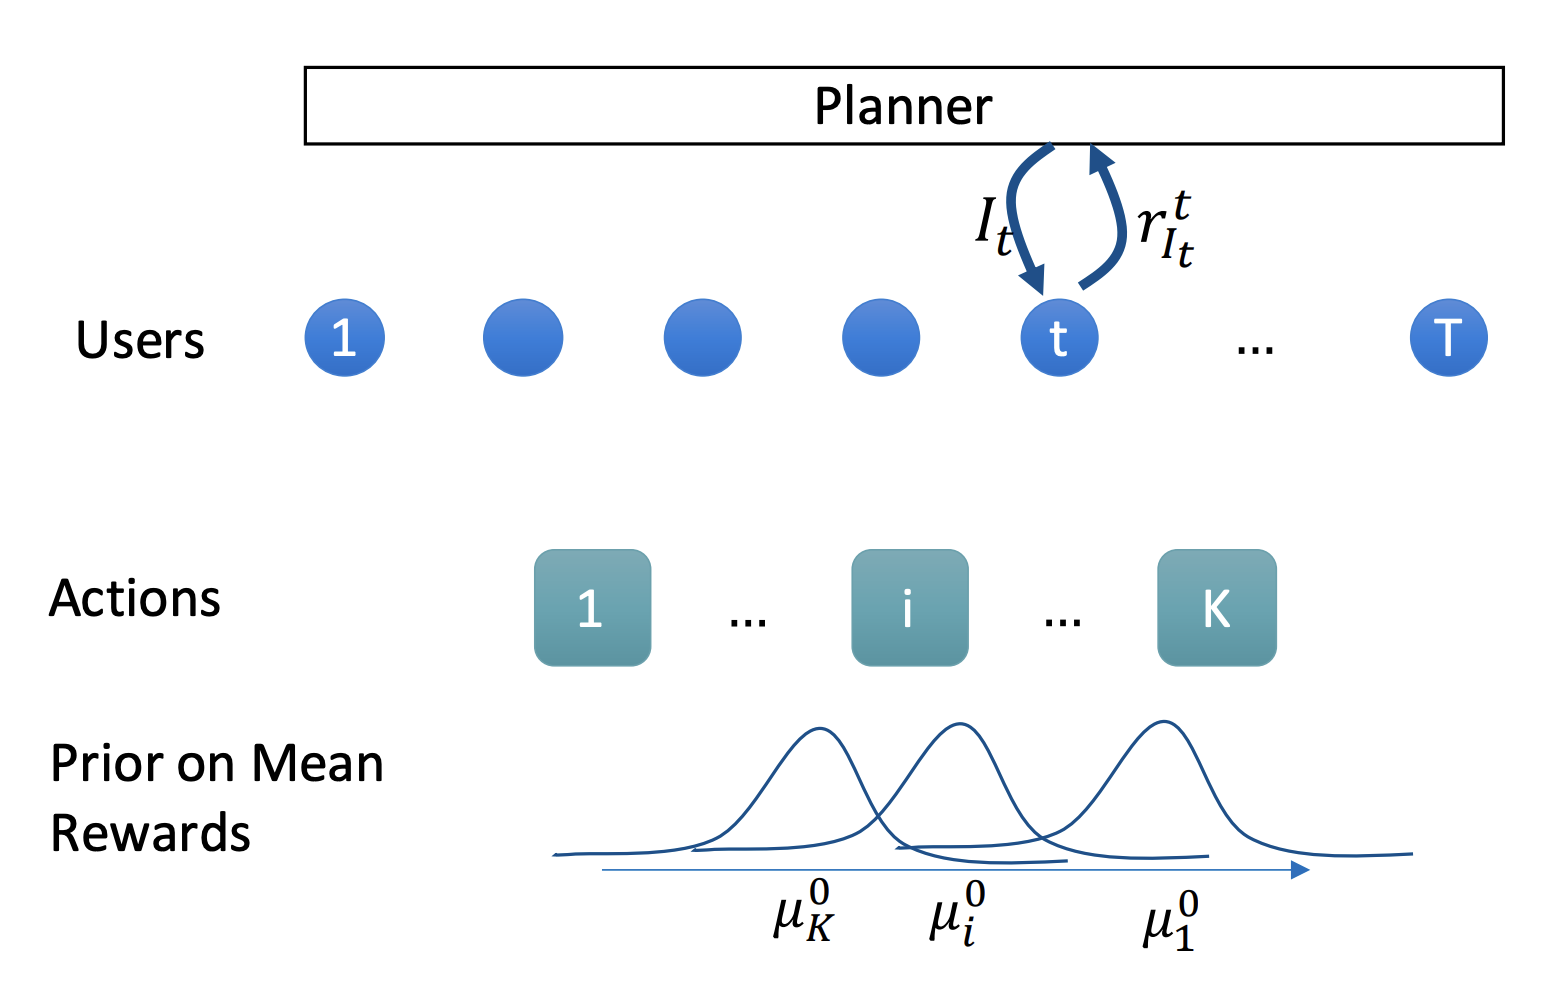
\includegraphics[width=0.6\textwidth,height=\textheight]{src/Figures/planner-agent-setup.png}

}

\caption{\label{fig-planner-agent}Planner-agent setup}

\end{figure}%

So far, the model we have defined is equivalent to a multi-armed bandit
model, which we have seen earlier in this chapter
(\hyperref[4optim]{1}). Under this model, well-known results in
economics, operations research and computer science show that
\(O(\sqrt{T})\) regret is achievable
(\citeproc{ref-russo2015informationtheoreticanalysisthompsonsampling}{Russo
and Roy 2015}; \citeproc{ref-auer_cesa-bianchi_fischer_2002}{Auer,
Cesa-Bianchi, and Fischer 2002}; \citeproc{ref-LAI19854}{Lai and Robbins
1985}) with algorithms such as Thompson sampling and UCB.

However, our agents are strategic and aim to maximize their own rewards.
If they observe the rewards gained from actions taken by other previous
users, they will simply take the action they believe will yield the
highest reward given the previous actions; they would prefer to benefit
from exploration done by other users rather than take the risk of
exploring themselves. Therefore, exploration on an individual level,
which the planner would like to facilitate, is not guaranteed under this
paradigm.

In light of this, we also require that our model satisfy
\textbf{incentive compatibility}, or that taking the action recommended
by the planner has an expected utility that is as high as any other
action the agent could take. Formally,
\[\forall i : \, E[\mu_i | I_t = i] \geq E[\mu_{i'} | I_t = i].\] Note
that this incentivizes the agents to actually take the actions
recommended by the planner; if incentive compatibility is not satisfied,
agents would simply ignore the planner and take whatever action they
think will lead to the highest reward.

At a high level, the key to achieving incentive compatibility while
still creating a policy for the planner that facilitates exploration is
information asymmetry. Under this paradigm, the users only have access
to their previous recommendations, actions, and rewards, and not to the
recommendations, actions, and rewards of other users. Therefore, they
are unsure of whether, after other users take certain actions and
receive certain rewards, arms that they might have initially considered
worse in practice outperform arms that they initially considered better.
Only the planner has access to the previous actions and rewards of all
users; the user only has access to their own recommendations and overall
knowledge of the planner's policy.

The main question we aim to answer for the rest of this section is,
given this new constraint of incentive compatibility, is \(O(\sqrt{T})\)
regret still achievable? We illustrate such an algorithm in the
following.

\subsubsection*{Black-box Reduction
Algorithm}\label{black-box-reduction-algorithm}
\addcontentsline{toc}{subsubsection}{Black-box Reduction Algorithm}

The main result for this chapter is a \textbf{black-box reduction}
algorithm to turn any bandit algorithm into an \emph{incentive
compatible} one, with only a constant increase in Bayesian regret.
Since, as mentioned earlier, there are bandit algorithms with
\(O(\sqrt{T})\) Bayesian regret, black-box reduction will also allow us
to get incentive-compatible algorithms with \(O(\sqrt{T})\) regret. The
idea of black-box reduction will be to simulate \(T\) steps of any
bandit algorithm in an incentive-compatible way in \(c T\) steps. This
allows us to design incentive-compatible recommendation systems by using
any bandit algorithm and then adapting it.

Consider the following setting: there are two possible actions, \(A_1\)
and \(A_2\). Assume the setting of \textbf{deterministic rewards}, where
action 1 has reward \(\mu_1\) with prior \(U[1/3, 1]\) and mean
\(\mathbb{E}[\mu_1] = 2/3\), and action 2 has reward \(\mu_2\) with
prior \(U[0, 1]\) and mean \(\mathbb{E}[\mu_2] = 1/2\). Without the
planner intervention and with full observability, users would simply
always pick \(A_1\), so how can the planner \emph{incentivize} users to
play \(A_2\)?

\begin{figure}

\centering{

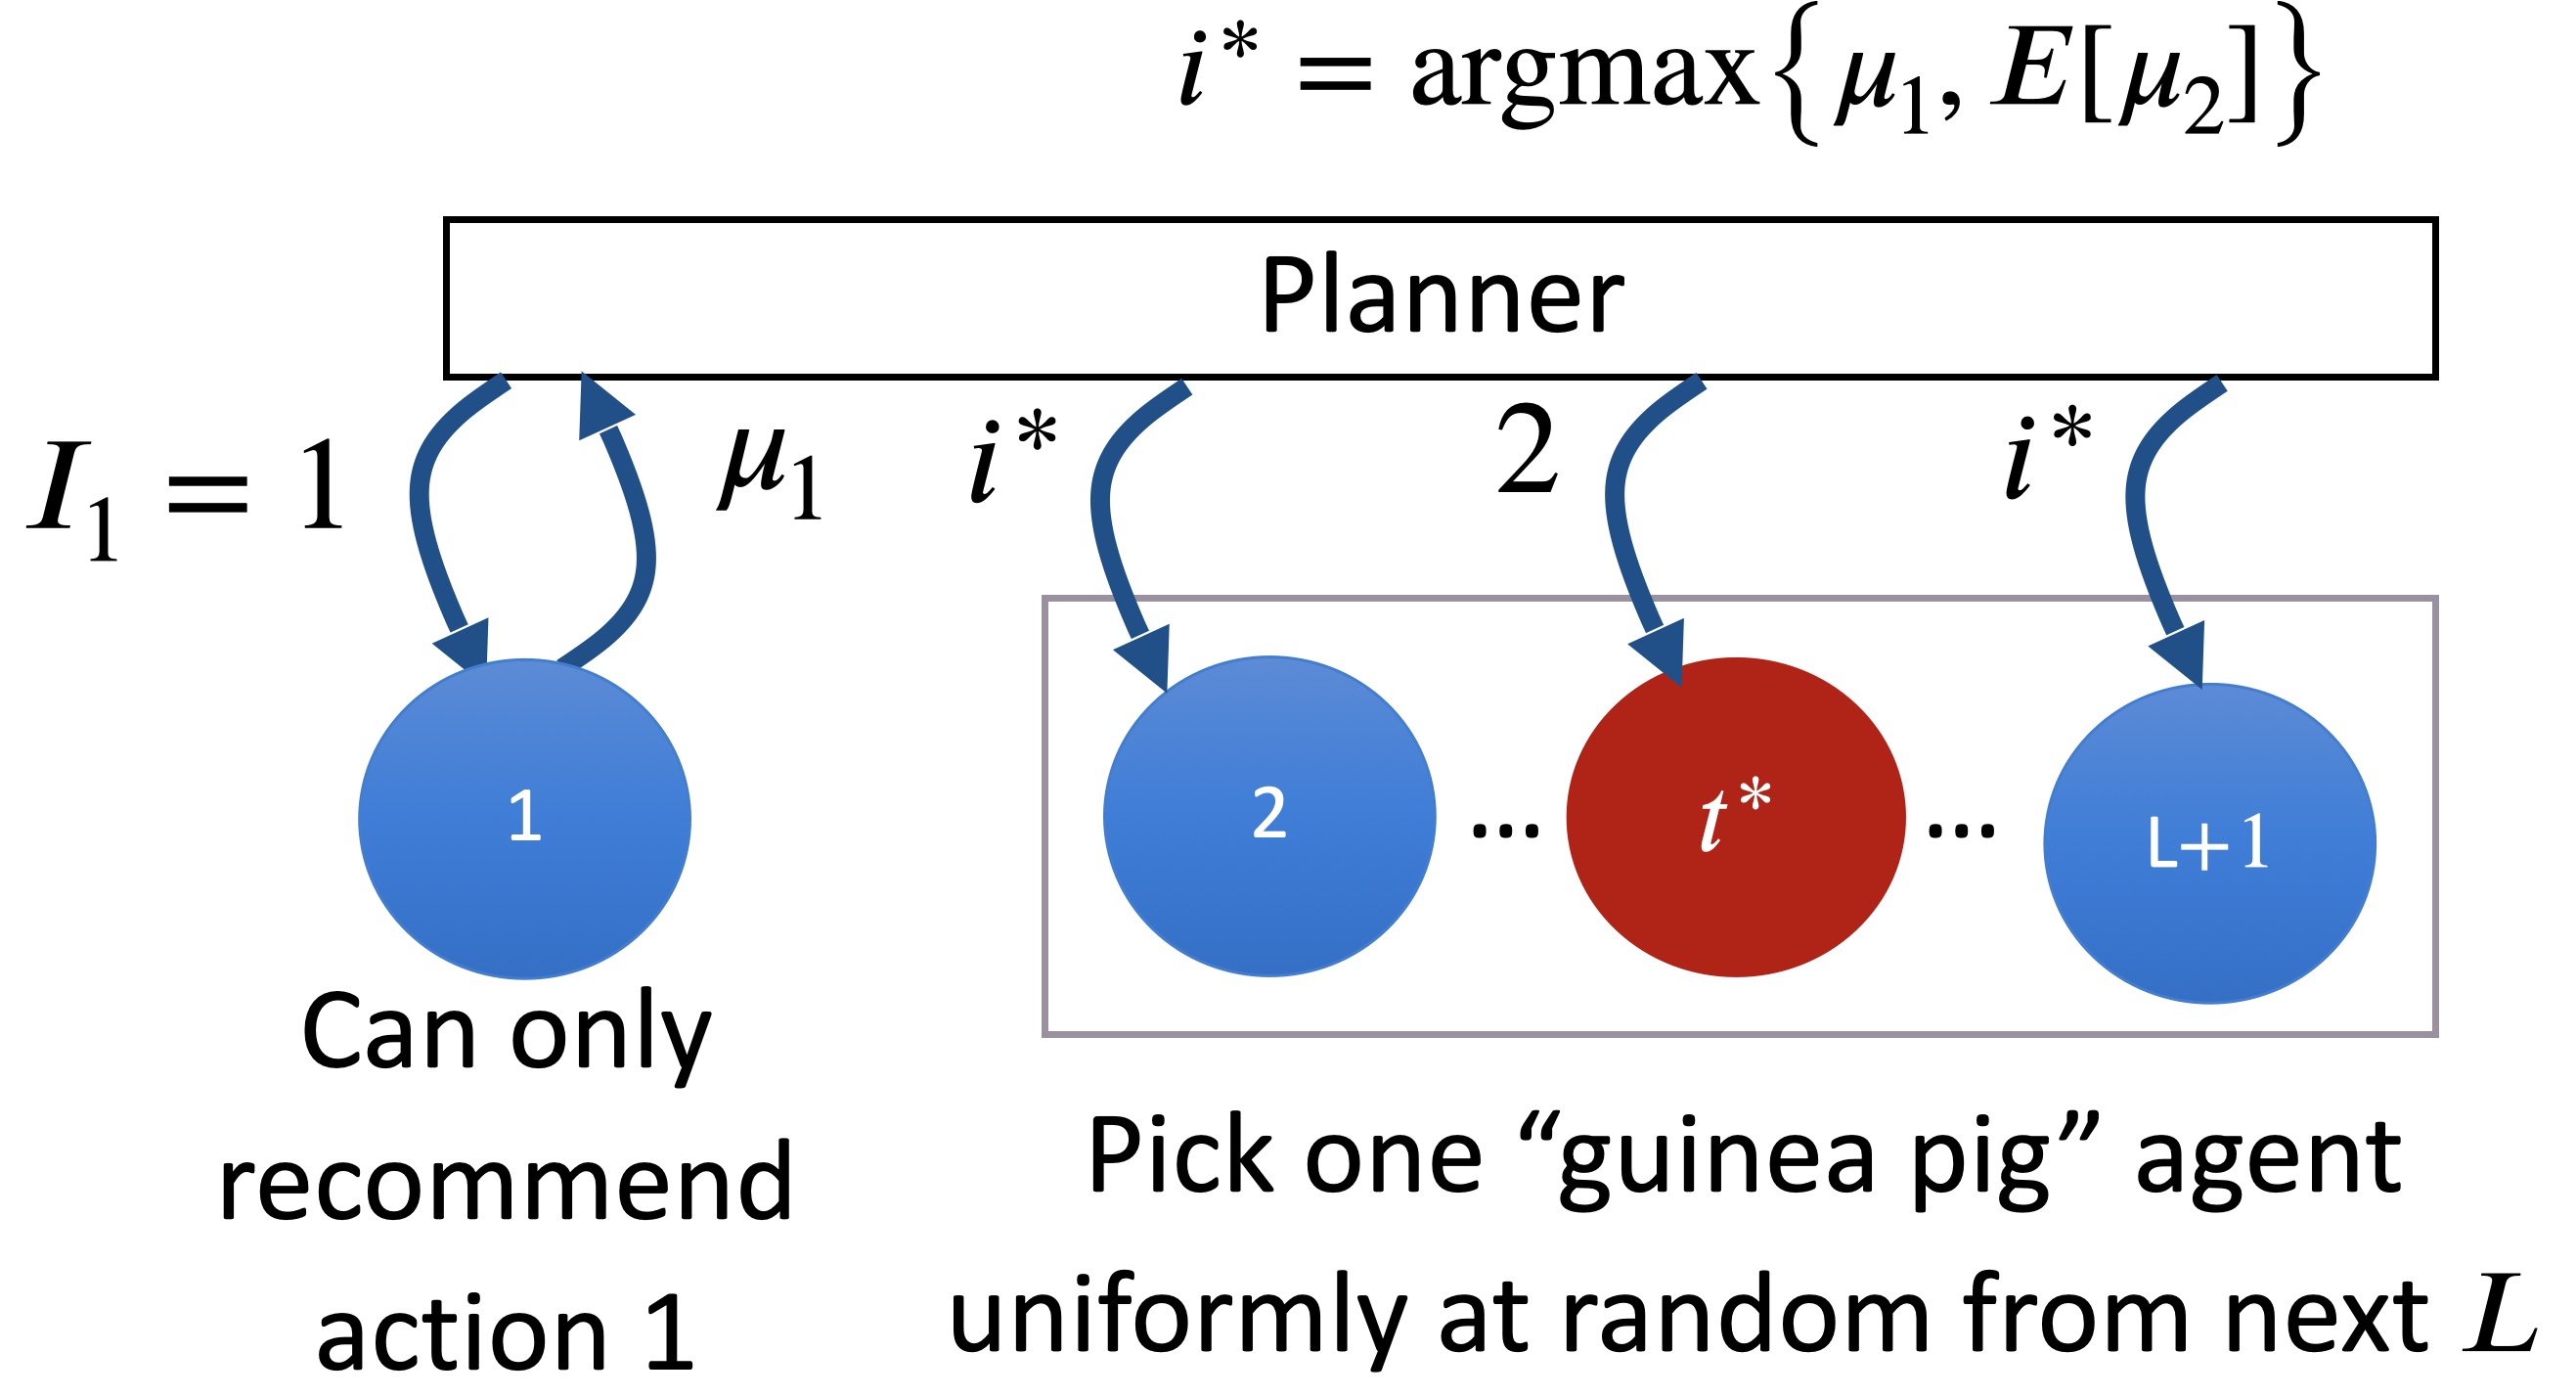
\includegraphics{src/Figures/guinea_pig_fig.png}

}

\caption{\label{fig-deterministic-guinea-pig}Illustration of black-box
reduction algorithm when we have deterministic rewards.}

\end{figure}%

The key insight is going to be to \emph{hide exploration in a pool of
exploitation}. The users are only going to receive a recommendation from
the planner, and no other observations. After deterministically
recommending the action with the highest expected reward (\(A_1\)), the
planner will pick one \textbf{guinea pig} to recommend the exploratory
action of \(A_2\). The users don't know whether they are the guinea pig,
so intuitively, as long as the planner picks guinea pigs uniformly at
random and at low enough frequencies, the optimal decision for the users
is still to follow the planner's recommendation, even if it might go
against their interest.

The planner will pick the user who will be recommended the exploratory
action uniformly at random from the \(L\) users that come after the
first one (which deterministically gets recommended the exploitation
action). Under this setting (illustrated in Figure
\hyperref[fig-deterministic-guinea-pig]{1.2}), it is optimal for users
to always follow the option that is recommended for them. More formally,
if \(I_t\) is the recommendation that a user receives at time \(t\),
then we have that: \[\begin{split}
    \mathbb{E}[\mu_1 - \mu_2 | I_t = 2] Pr[I_t = 2] &= \frac{1}{L} (\mu_1 - \mu_2) \quad \text{(Gains if you are the unlucky guinea pig)}\\
    &+ (1 - \frac{1}{L}) \mathbb{E}[\mu_1 - \mu_2 | \mu_1 < \mu_2] Pr[\mu_1 < \mu_2] \quad \text{(Loss if you are not and $\mu_1 < \mu_2$)}\\
    &\leq 0
\end{split}\] This holds when \(L \geq 12\). It means that the gains
from not taking the recommended action are \emph{negative}, which
implies that users should always take the recommendation.

So far we have considered the case where rewards are deterministic, but
what about \textbf{stochastic rewards}? We are now going to consider the
case where rewards are independent and identically distributed from some
distribution, and where each action \(A_i\) has some reward distribution
\(r_i^t \sim D_i, \mathbb{E}[r_i^t] = \mu_i\). Back to the case where
there are only two actions, we are going to adapt the prior algorithm of
guinea pig-picking to the stochastic reward setting. Since one reward
observation is not enough to fully know \(\mu_1\) anymore, we'll instead
observe the outcome of the first action \(M\) times to form a strong
posterior \(\mathbb{E}[\mu_1 | r_1^1, \ldots r_1^M]\).

\begin{figure}

\centering{

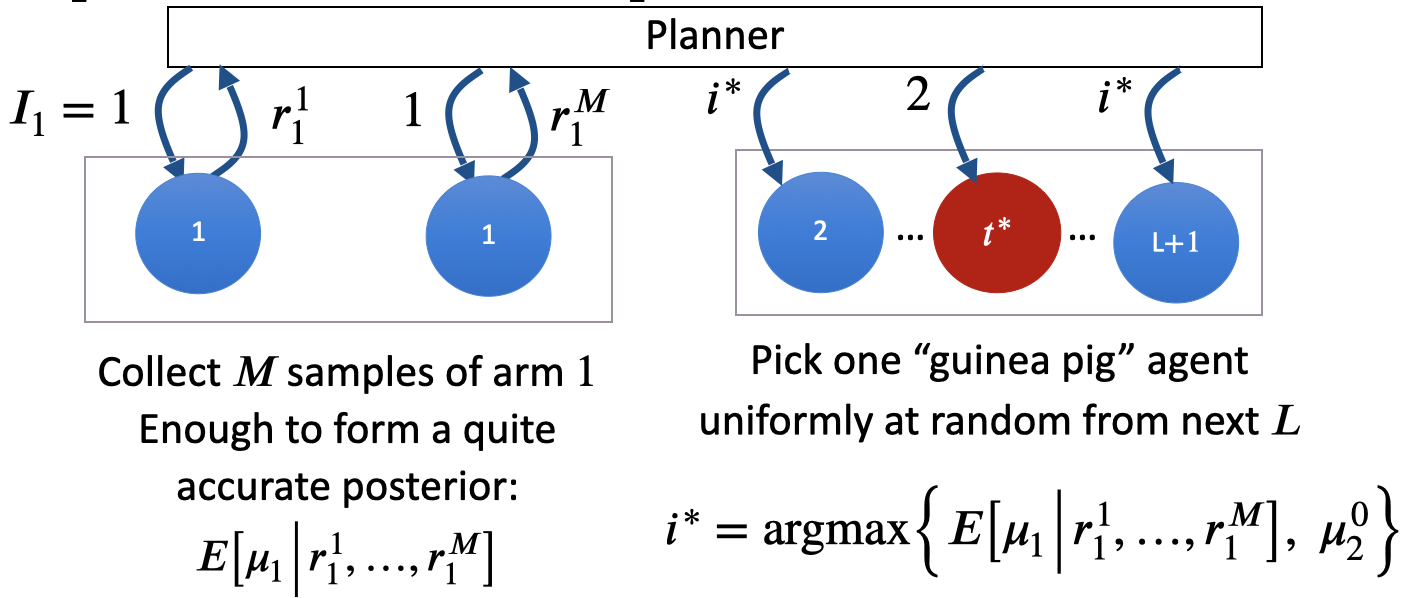
\includegraphics{src/Figures/stochastic_guinea_pig.png}

}

\caption{\label{fig-stochastic-guinea-pig}Illustration of black-box
reduction algorithm when we have stochastic rewards.}

\end{figure}%

Figure \hyperref[fig-stochastic-guinea-pig]{1.3} illustrates the
algorithm that we can use with stochastic rewards when there are two
actions. Similarly, as before, we pick one guinea pig uniformly at
random from the next \(L\) users and use the reward we get as the
exploratory signal.\\
In a very similar manner, we can generalize this algorithm from always
having two actions to the general multi-armed bandit problem. Now
suppose we have a general multi-armed bandit algorithm \(A\). We will
wrap this algorithm around our black box reduction algorithm to make it
incentive-compatible.

\begin{figure}

\centering{

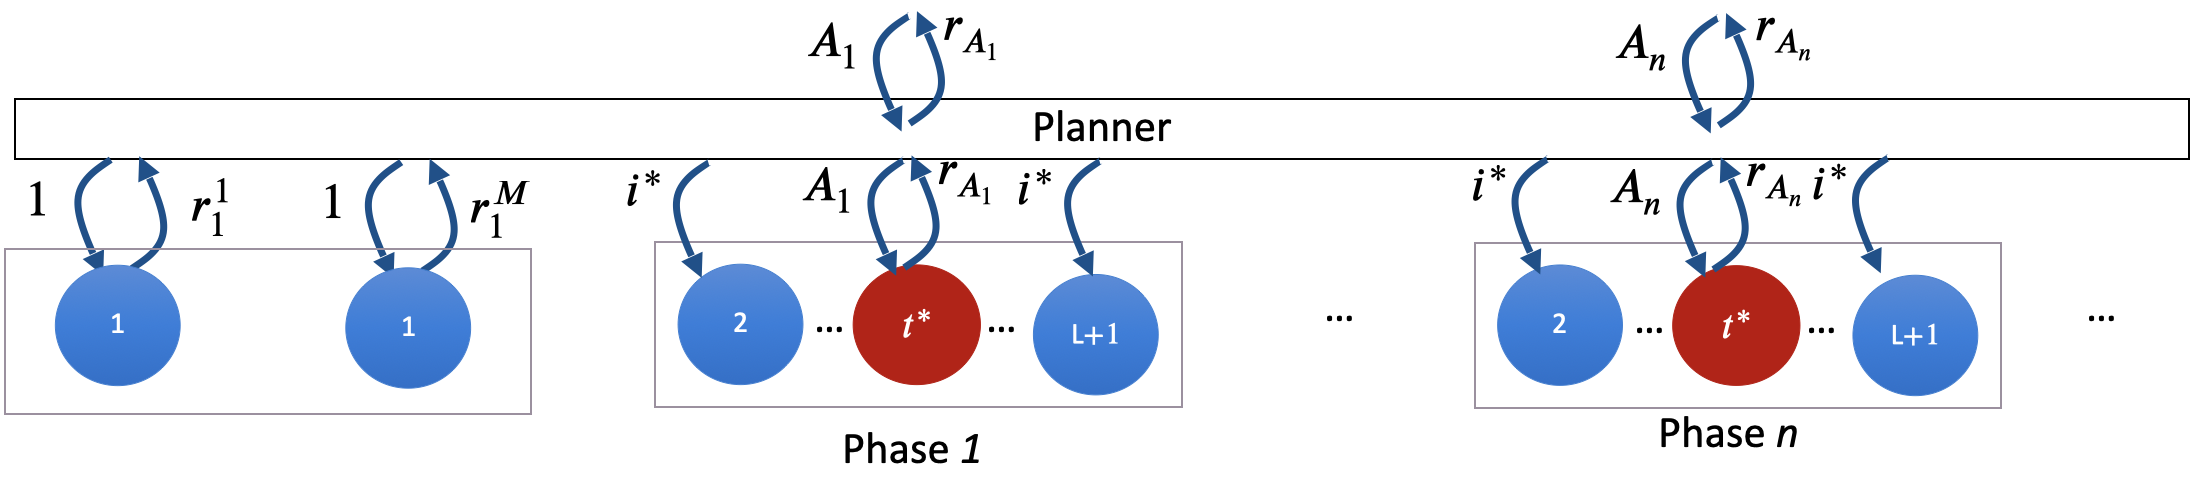
\includegraphics{src/Figures/multi-armed-guinea-pig.png}

}

\caption{\label{fig-multi-armed-guinea-pig}Illustration of black-box
reduction algorithm for the general multi-armed bandit case.}

\end{figure}%

As Figure \hyperref[fig-multi-armed-guinea-pig]{1.4} shows, we wrap
every decision that \(A\) would make by exactly \(L-1\) recommendations
of the action believed to be the best so far. This guarantees that the
expected rewards for the users that are not chosen as guinea pigs are at
least as good as \(A\)'s reward at phase \(n\).

\section{Preferential Bayesian
Optimization}\label{preferential-bayesian-optimization}

The traditional Bayesian optimization (BO) problem is described as
follows. There is a black-box objective function
\(g: \mathcal{X} \rightarrow \Re\) defined on a bounded subset
\(\mathcal{X} \subseteq \Re^q\) such that direct queries to the function
are expensive or not possible. However, we would like to solve the
global optimization problem of finding
\(\mathbf{x}_{\min }=\arg \min _{\mathbf{x} \in \mathcal{X}} g(\mathbf{x})\).
This is highly analogous to modeling human preferences, since it is the
case that direct access to a human's latent preference function is not
possible but we would still like to find its optimum, such as in A/B
tests or recommender systems.

We approach this problem for human preferences with \emph{Preferential
Bayesian Optimization} (PBO), as the key difference is that we are able
to query the preference function through pairwise comparisons of data
points, i.e.~\emph{duels}. This is a form of indirect observation of the
objective function, which models real-world scenarios closely: we
commonly need to to optimize a function via data about preferences. With
humans, it has been demonstrated that we are better at evaluating
differences rather than absolute magnitudes
(\citeproc{ref-kahneman_tversky_1979}{Kahneman and Tversky 1979}) and
therefore PBO models can be applied in various contexts.

\subsection{Problem statement}\label{problem-statement}

The problem of finding the optimum of a latent preference function
defined on \(\mathcal{X}\) can be reduced to determining a sequence of
duels on \(\mathcal{X} \times \mathcal{X}\). From each duel
\(\left[\mathbf{x}, \mathbf{x}^{\prime}\right] \in\)
\(\mathcal{X} \times \mathcal{X}\) we obtain binary feedback \(\{0,1\}\)
indicating whether or not \(\mathbf{x}\) is preferred over
\(\mathbf{x}^{\prime}\) (\(g(\mathbf{x}) < g(\mathbf{x}^{\prime})\)). We
consider that \(\mathbf{x}\) is the winner of the duel if the output is
\(\{1\}\) and that \(\mathbf{x}^{\prime}\) wins the duel if the output
is \(\{0\}\). The aim is to find \(\mathbf{x}_{\min }\) by reducing as
much as possible the number of queried duels.

The key idea in PBO is to learn a preference function in the space of
duels using a Gaussian process. We define a joint reward
\(f\left(\left[\mathbf{x}, \mathbf{x}^{\prime}\right]\right)\) on each
duel which is never directly observed. Instead, the feedback we obtain
after each pair is a binary output \(y \in\) \(\{0,1\}\) indicating
which of the two inputs is preferred. One definition of f we will use
(though others are possible) is
\(f\left(\left[\mathbf{x}, \mathbf{x}^{\prime}\right]\right)=g\left(\mathbf{x}^{\prime}\right)-g(\mathbf{x})\).
The more \(\mathbf{x}^{\prime}\) is preferred over \(\mathbf{x}\), the
bigger the reward.

We define the model of preference using a Bernoulli likelihood, where
\(p\left(y=1 \mid\left[\mathbf{x}, \mathbf{x}^{\prime}\right]\right)=\pi_f\left(\left[\mathbf{x}, \mathbf{x}^{\prime}\right]\right)\)
and
\(p\left(y=0 \mid\left[\mathbf{x}, \mathbf{x}^{\prime}\right]\right)=\pi_f\left(\left[\mathbf{x}^{\prime}, \mathbf{x}\right]\right)\)
for some inverse link function \(\pi: \Re \times \Re \rightarrow[0,1]\).
\(\pi_f\) has the property that
\(\pi_f\left(\left[\mathbf{x}^{\prime}, \mathbf{x}\right]\right)=1-\pi_f\left(\left[\mathbf{x}, \mathbf{x}^{\prime}\right]\right)\).
A natural choice for \(\pi_f\) is the logistic function
\[\label{eq:bernoulli_pref}
\pi_f\left(\left[\mathbf{x}, \mathbf{x}^{\prime}\right]\right)=\sigma\left(f\left(\left[\mathbf{x}, \mathbf{x}^{\prime}\right]\right)\right)=\frac{1}{1+e^{-f\left(\left[\mathbf{x}, \mathbf{x}^{\prime}\right]\right)}},\]
but others are possible. Therefore we have that for any duel
\(\left[\mathbf{x}, \mathbf{x}^{\prime}\right]\) in which
\(g(\mathbf{x}) \leq g\left(\mathbf{x}^{\prime}\right)\) it holds that
\(\pi_f\left(\left[\mathbf{x}, \mathbf{x}^{\prime}\right]\right) \geq 0.5\).
\(\pi_f\) is a preference function that maps each query
\(\left[\mathbf{x}, \mathbf{x}^{\prime}\right]\) to the probability of
having a preference on the left input \(\mathbf{x}\) over the right
input \(\mathbf{x}^{\prime}\).

When we marginalize over the right input \(\mathbf{x}^{\prime}\) of
\(f\) (is this correct?), the global minimum of \(f\) in \(\mathcal{X}\)
coincides with \(\mathbf{x}_{\min }\). We also introduce the definition
of the \emph{Copeland score function} for a point \(\mathbf{x}\) as
\[S(\mathbf{x})=\operatorname{Vol}(\mathcal{X})^{-1} \int_{\mathcal{X}} \mathbb{I}_{\left\{\pi_f\left(\left[\mathbf{x}, \mathbf{x}^{\prime}\right]\right) \geq 0.5\right\}} d \mathbf{x}^{\prime}\]
where
\(\operatorname{Vol}(\mathcal{X})=\int_{\mathcal{X}} d \mathbf{x}^{\prime}\)
is a normalizing constant that bounds \(S(\mathbf{x})\) in the interval
\([0,1]\). If \(\mathcal{X}\) is a finite set, the Copeland score is
simply the proportion of duels that a certain element \(\mathbf{x}\)
will win with probability larger than 0.5. A soft variant we will use
instead of the Copeland score is the \emph{soft-Copeland score}, defined
as \[\label{eq:soft-copeland}
C(\mathbf{x})=\operatorname{Vol}(\mathcal{X})^{-1} \int_{\mathcal{X}} \pi_f\left(\left[\mathbf{x}, \mathbf{x}^{\prime}\right]\right) d \mathbf{x}^{\prime}\]
where the probability function \(\pi_f\) is integrated over
\(\mathcal{X}\). This score aims to capture the average probability of
\(\mathbf{x}\) being the winner of a duel.

We define the \emph{Condorcet winner} \(\mathbf{x}_c\) as the point with
maximal soft-Copeland score. Note that this corresponds to the global
minimum of \(f\), since the defining integral takes maximum value for
points \(\mathbf{x} \in \mathcal{X}\) where
\(f\left(\left[\mathbf{x}, \mathbf{x}^{\prime}\right]\right)=\)
\(g\left(\mathbf{x}^{\prime}\right)-g(\mathbf{x})>0\) or all
\(\mathbf{x}^{\prime}\), occurring only if \(\mathbf{x}_c\) is a minimum
of \(f\). Therefore, if the preference function \(\pi_f\) can be learned
by observing the results of duels then our optimization problem of
finding the minimum of \(f\) can be solved by finding the Condorcet
winner of the Copeland score.

\subsection{Acquisition Functions}\label{acquisition-functions-1}

We describe several acquisition functions for sequential learning of the
Condorcet winner. Our dataset
\(\mathcal{D}=\left\{\left[\mathbf{x}_i, \mathbf{x}_i^{\prime}\right], y_i\right\}_{i=1}^N\)
represents the \(N\) duels that have been performed so far. We aim to
define a sequential policy
\(\alpha\left(\left[\mathbf{x}, \mathbf{x}^{\prime}\right] ; \mathcal{D}_j, \theta\right)\)
for querying duels, where \(\theta\) is a vector of model
hyper-parameters, in order to find the minimum of the latent function
\(g\) as quickly as possible. Using Gaussian processes (GP) for
classification with our dataset \(\mathcal{D}\) allows us to perform
inference over \(f\) and \(\pi_f\).

\subsubsection*{Pure Exploration}\label{pure-exploration}
\addcontentsline{toc}{subsubsection}{Pure Exploration}

The output variable \(y_{\star}\) of a prediction follows a Bernoulli
distribution with probability given by the preference function
\(\pi_f\). To carry out exploration as a policy, one method is to search
for the duel where GP is most uncertain about the probability of the
outcome (has the highest variance of \(\sigma\left(f_{\star}\right)\) ),
which is the result of transforming out epistemic uncertainty about
\(f\), modeled by a GP, through the logistic function. The first order
moment of this distribution coincides with the expectation of
\(y_{\star}\) but its variance is \[\begin{aligned}
\mathbb{V}\left[\sigma\left(f_{\star}\right)\right] & =\int\left(\sigma\left(f_{\star}\right)-\mathbb{E}\left[\sigma\left(f_{\star}\right)\right]\right)^2 p\left(f_{\star} \mid \mathcal{D},\left[\mathbf{x}, \mathbf{x}^{\prime}\right]\right) d f_{\star} \\
& =\int \sigma\left(f_{\star}\right)^2 p\left(f_{\star} \mid \mathcal{D},\left[\mathbf{x}, \mathbf{x}^{\prime}\right]\right) d f_{\star}-\mathbb{E}\left[\sigma\left(f_{\star}\right)\right]^2
\end{aligned}\] which explicitly takes into account the uncertainty over
\(f\). Hence, pure exploration of duels space can be carried out by
maximizing
\[\alpha_{\mathrm{PE}}\left(\left[\mathbf{x}, \mathbf{x}^{\prime}\right] \mid \mathcal{D}_j\right)=\mathbb{V}\left[\sigma\left(f_{\star}\right)\left|\left[\mathbf{x}_{\star}, \mathbf{x}_{\star}^{\prime}\right]\right| \mathcal{D}_j\right] .\]

Note that in this case, duels that have been already visited will have a
lower chance of being visited again even in cases in which the objective
takes similar values in both players. In practice, this acquisition
functions requires computation of an intractable integral, that we
approximate using Monte-Carlo.

\subsubsection*{Principled Optimistic Preferential Bayesian Optimization
(POP-BO)}\label{principled-optimistic-preferential-bayesian-optimization-pop-bo}
\addcontentsline{toc}{subsubsection}{Principled Optimistic Preferential
Bayesian Optimization (POP-BO)}

In a slightly modified problem setup
(\citeproc{ref-xu2024principledpreferentialbayesianoptimization}{Xu et
al. 2024}), the algorithm tries to solve for the MLE \(\hat{g}\) and its
confidence set \(\mathcal{B}_g\) where \(g\) is the ground truth
black-box function. Assumptions include that \(g\) is a member of a
reproducing kernel Hilbert space (RKHS) \(\mathcal{H}_k\) for some
kernel function
\(k: \mathbb{R}^d \times \mathbb{R}^d \rightarrow \mathbb{R}\), and
\(\|g\|_k \leq B\) so that
\(\mathcal{B}_g = \left\{\tilde{g} \in \mathcal{H}_k \mid\|\tilde{g}\|_k \leq B\right\}\).
Similarly defining
\(f\left(\left[\mathbf{x}, \mathbf{x}^{\prime}\right]\right)=g\left(\mathbf{x}^{\prime}\right)-g(\mathbf{x})\),
we model the preference function with a Bernoulli distribution as in
Equation \hyperref[eq:bernoulli_pref]{{[}eq:bernoulli\_pref{]}} and also
assume that probabilities follow the Bradley-Terry model, i.e.
\[\pi_f\left(\left[\mathbf{x}, \mathbf{x}^{\prime}\right]\right)=\sigma\left(f\left(\left[\mathbf{x}, \mathbf{x}^{\prime}\right]\right)\right)=\frac{e^{g(\mathbf{x})}}{e^{g(\mathbf{x})}+e^{g\left(\mathbf{x^{\prime}}\right)}}\]

The update rule for MLE \(\hat{g}\) is (equation 8,6,5)
\[\begin{aligned}
\hat{g}_t^{\text {MLE }}&:= \arg \underset{\tilde{g} \in \mathcal{B}^t_g}{\max}\ell_t(\tilde{g}) \\
\ell_t(\tilde{g}) &:= \log \prod_{\tau=1}^t y_\tau \pi_{\tilde{f}}([\mathbf{x_\tau}, \mathbf{x^{\prime}_\tau}])+\left(1-y_\tau\right)\left(1-\pi_{\tilde{f}}([\mathbf{x_\tau}, \mathbf{x^{\prime}_\tau}])\right) \\
&=\sum_{\tau=1}^t \log \left(\frac{e^{\tilde{g}(\mathbf{x_\tau})} y_\tau+e^{\tilde{g}(\mathbf{x_\tau^\prime})}\left(1-y_\tau\right)}{e^{\tilde{g}(\mathbf{x_\tau})}+e^{\tilde{g}(\mathbf{x_\tau^\prime})}}\right) \\
&=\sum_{\tau=1}^t\left(\tilde{g}(\mathbf{x_\tau}) y_\tau+\tilde{g}(\mathbf{x_\tau^\prime})\left(1-y_\tau\right)\right)-\sum_{\tau=1}^t \log \left(e^{\tilde{g}(\mathbf{x_\tau})}+e^{\tilde{g}(\mathbf{x_\tau^\prime})}\right)
\end{aligned}\]

(Eq 22 shows how to represent this as a convex optimisation problem so
that it can be solved)

The update rule for the confidence set \(\mathcal{B}_f^{t+1}\) is, (eq
9, 10?)

\[\begin{aligned}
&\forall \epsilon, \delta > 0 \\
&\mathcal{B}_g^{t+1}:=\left\{\tilde{g} \in \mathcal{B}_g \mid \ell_t(\tilde{g}) \geq \ell_t\left(\hat{g}_t^{\mathrm{MLE}}\right)-\beta_1(\epsilon, \delta, t)\right\}
\end{aligned}\] where
\[\beta_1(\epsilon, \delta, t):=\sqrt{32 t B^2 \log \frac{\pi^2 t^2 \mathcal{N}\left(\mathcal{B}_f, \epsilon,\|\cdot\|_{\infty}\right)}{6 \delta}}+ C_L \epsilon t=\mathcal{O}\left(\sqrt{t \log \frac{t \mathcal{N}\left(\mathcal{B}_f, \epsilon,\|\cdot\|_{\infty}\right)}{\delta}}+\epsilon t\right),\]
with \(C_L\) a constant independent of \(\delta, t\) and \(\epsilon\).
\(\epsilon\) is typically chosen to be \(1 / T\), where T is the running
horizon of the algorithm. This satisfies the theorem that,
\[\mathbb{P}\left(g \in \mathcal{B}_g^{t+1}, \forall t \geq 1\right) \geq 1-\delta .\]

Intuitively, the confidence set \(\mathcal{B}_g^{t+1}\) includes the
functions with the log-likelihood value that is only `a little worse'
than the maximum likelihood estimator, and the theorem states that
\(\mathcal{B}_g^{t+1}\) contains the ground-truth function \(g\) with
high probability.

Inner level optimization in Line 4 of the algorithm can also be
represented as a convex optimisation problem so that it can be solved,
Eq 24, 25. The outer optimisation can be solved using grid search or Eq
26 for medium size problems.

Given the initial point \(\mathbf{x_0} \in \mathcal{X}\) and set
\(\mathcal{B}_g^1 = \mathcal{B}_g\) Set the reference point
\(\mathbf{x_t^{\prime}} = \mathbf{x_{t-1}}\) Compute
\(\mathbf{x_t} \in \arg\max_{\mathbf{x} \in \mathcal{X}} \max_{\tilde{g} \in \mathcal{B}_g^t} (\tilde{g}(\mathbf{x}) - \tilde{g}(\mathbf{x_t^{\prime}}))\),
with the inner optimal function denoted as \(\tilde{g}_t\) Obtain the
output of the duel \(y_t\) and append the new data point to
\(\mathcal{D}_t\) Update the maximum likelihood estimator
\(\hat{g}_t^{\mathrm{MLE}}\) and the posterior confidence set
\(\mathcal{B}_g^{t+1}\).

\subsubsection*{qEUBO: Decision-Theoretic
EUBO}\label{qeubo-decision-theoretic-eubo}
\addcontentsline{toc}{subsubsection}{qEUBO: Decision-Theoretic EUBO}

qEUBO
(\citeproc{ref-astudillo2023qeubodecisiontheoreticacquisitionfunction}{Astudillo
et al. 2023}) derives an acquisition function that extends duels to
\(q>2\) options which we call \emph{queries}. Let
\(X=\left(\mathbf{x_1}, \ldots, \mathbf{x_q}\right) \in \mathcal{X}^q\)
denote a query containing two points or more, and let
\(g: \mathcal{X} \rightarrow \Re\) be the latent preference function.
Then after \(n\) user queries, we define the \emph{expected utility of
the best option} (qEUBO) as
\[\mathrm{qEUBO}_n(X)=\mathbb{E}_n\left[\max \left\{g\left(x_1\right), \ldots, g\left(x_q\right)\right\}\right].\]

We now show that qEUBO is one-step Bayes optimal, meaning that each step
chooses the query that maximises the expected utility received by the
human. For a query \(X \in \mathcal{X}^q\), let
\[V_n(X)=\mathbb{E}_n\left[\max _{x \in \mathbb{X}} \mathbb{E}_{n+1}[g(x)] \mid X_{n+1}=X\right] .\]
Then \(V_n\) defines the expected utility received if an additional
query \(X_{n+1}=X\) is performed, and maximizing \(V_n\) is one-step
Bayes optimal. Since \(\max _{x \in \mathbb{X}} \mathbb{E}_n[f(x)]\)
does not depend on \(X_{n+1}\), we can also equivalently maximize
\[\mathbb{E}_n\left[\max _{x \in \mathbb{X}} \mathbb{E}_{n+1}[g(x)]-\max _{x \in \mathbb{X}} \mathbb{E}_n[g(x)] \mid X_{n+1}=X\right],\]
which takes the same form as the knowledge gradient acquisition function
(\citeproc{ref-wu2018parallelknowledgegradientmethod}{Wu and Frazier
2018}) in standard Bayesian optimization.

\(V_n\) involves a nested stochastic optimization task, while qEUBO is a
much simpler policy. When human responses are noise-free, we are able to
use qEUBO as a sufficient policy due to the following theorem:

\[\underset{X \in \mathbb{X}^q}{\operatorname{argmax}} \mathrm{qEUBO}_n(X) \subseteq \underset{X \in \mathbb{X}^q}{\operatorname{argmax}} V_n(X) .\]

\begin{proof}
\emph{Proof.} For a query \(X \in \mathcal{X}^q\), let
\(x^{+}(X, i) \in \operatorname{argmax}_{x \in \mathbb{X}} \mathbb{E}_n[g(x) \mid(X, i)]\)
and define \(X^{+}(X)=\)
\(\left(x^{+}(X, 1), \ldots, x^{+}(X, q)\right)\).

\textbf{Claim 1} \(V_n(X) \leq \mathrm{qEUBO}_n\left(X^{+}(X)\right) .\)
We see that \[\begin{aligned}
V_n(X) & =\sum_{i=1}^q \mathbf{P}_n(r(X)=i) \mathbb{E}_n[g\left(x^{+}(X, i)\right) ] \\
& \leq \sum_{i=1}^q \mathbf{P}_n(r(X)=i) \mathbb{E}_n[\max _{i=1, \ldots, q} g(x^{+}(X, i))] \\
& =\mathbb{E}_n\left[\max _{i=1, \ldots, q} g\left(x^{+}(X, i)\right)\right] \\
& =\mathrm{qEUBO}_n\left(X^{+}(X)\right),
\end{aligned}\] as claimed.

\textbf{Claim 2} \(\mathrm{qEUBO}_n(X) \leq V_n(X) .\) For any given
\(X \in \mathbb{X}^q\) we have
\[\mathbb{E}_n\left[f\left(x_{r(X)}\right) \mid(X, r(X))\right] \leq \max _{x \in \mathbb{X}} \mathbb{E}_n[f(x) \mid(X, r(X))] .\]
Since
\(f\left(x_{r(X)}\right)=\max _{i=1, \ldots, q} f\left(x_i\right)\),
taking expectations over \(r(X)\) on both sides obtains the required
result.

Now building on the arguments above, let
\(X^* \in \operatorname{argmax}_{X \in \mathbb{X}^q} \mathrm{qEUBO}_n(X)\)
and suppose for contradiction that
\(X^* \notin \operatorname{argmax}_{X \in \mathbb{X}^q} V_n(X)\). Then,
there exists \(\widetilde{X} \in \mathbb{X}^q\) such that
\(V_n(\widetilde{X})>V_n\left(X^*\right)\). We have \[\begin{aligned}
\operatorname{qEUBO}_n\left(X^{+}(\tilde{X})\right) & \geq V_n(\tilde{X}) \\
& >V_n\left(X^*\right) \\
& \geq \operatorname{qEUBO}_n\left(X^*\right) \\
& \geq \operatorname{qEUBO}_n\left(X^{+}(\tilde{X})\right) .
\end{aligned}\]

The first inequality follows from (1). The second inequality is due to
our supposition for contradiction. The third inequality is due to (2).
Finally, the fourth inequality holds since
\(X^* \in \operatorname{argmax}_{X \in \mathbb{X}^q} \mathrm{qEUBO}_n(X)\).
This contradiction concludes the proof. ◻
\end{proof}

Therefore a sufficient condition for following one-step Bayes optimality
is by maximizing \(\text{qEUBO}_n\).

In experiments that were ran comparing qEUBO to other state-of-the-art
acquisition functions, qEUBO consistently outperformed on most problems
and was closely followed by qEI and qTS. These results also extended to
experiments with multiple options when \(q>2\). In fact, there is faster
convergence in regret when using more options in human queries. {[}Prove
Theorem 3: Regret analysis{]}

\subsubsection*{qEI: Batch Expected
Improvement}\label{qei-batch-expected-improvement}
\addcontentsline{toc}{subsubsection}{qEI: Batch Expected Improvement}

\[\begin{aligned}
\mathrm{qEI}= & \mathbb{E}_{\mathbf{y}}\left[\left(\max _{i \in[1, \ldots, q]}\left(\mu_{\min }-y_i\right)\right)_{+}\right] \\
= & \sum_{i=1}^q \mathbb{E}_{\mathbf{y}}\left(\mu_{\min }-y_i \mid y_i \leq \mu_{\min }, y_i \leq y_j \forall j \neq i\right) \\
& p\left(y_i \leq \mu_{\min }, y_i \leq y_j \forall j \neq i\right) .
\end{aligned}\]

\subsubsection*{qTS: Batch Thompson
Sampling}\label{qts-batch-thompson-sampling}
\addcontentsline{toc}{subsubsection}{qTS: Batch Thompson Sampling}

Initial data
\(\mathcal{D}_{\mathcal{I}(1)}=\{(\mathbf{x}_i, y_i)\}_{i \in \mathcal{I}(1)}\)
Compute current posterior
\(p(\boldsymbol{\theta} \mid \mathcal{D}_{\mathcal{I}(t)})\) Sample
\(\boldsymbol{\theta}\) from
\(p(\boldsymbol{\theta} \mid \mathcal{D}_{\mathcal{I}(t)})\) Select
\(k \leftarrow \arg \max_{j \notin \mathcal{I}(t)} \mathbb{E}[y_j \mid \mathbf{x}_j, \boldsymbol{\theta}]\)
Collect \(y_k\) by evaluating \(f\) at \(\mathbf{x}_k\)
\(\mathcal{D}_{\mathcal{I}(t+1)} \leftarrow \mathcal{D}_{\mathcal{I}(t)} \cup \{(\mathbf{x}_k, y_k)\}\)

Initial data
\(\mathcal{D}_{\mathcal{I}(1)}=\{\mathbf{x}_i, y_i\}_{i \in \mathcal{I}(1)}\),
batch size \(S\) Compute current posterior
\(p(\boldsymbol{\theta} \mid \mathcal{D}_{\mathcal{I}(t)})\) Sample
\(\boldsymbol{\theta}\) from
\(p(\boldsymbol{\theta} \mid \mathcal{D}_{\mathcal{I}(t)})\) Select
\(k(s) \leftarrow \arg \max_{j \notin \mathcal{I}(t)} \mathbb{E}[y_j \mid \mathbf{x}_j, \boldsymbol{\theta}]\)
\(\mathcal{D}_{\mathcal{I}(t+1)} = \mathcal{D}_{\mathcal{I}(t)} \cup \{\mathbf{x}_{k(s)}, y_{k(s)}\}_{s=1}^S\)

\subsection{Regret Analysis}\label{regret-analysis}

\subsubsection*{qEUBO Regret}\label{qeubo-regret}
\addcontentsline{toc}{subsubsection}{qEUBO Regret}

With the definition of Bayesian simple regret, we have that qEUBO
converges to zero at a rate of \(o(1/n)\), i.e.

\[\label{th:quebo_regret}
\mathbb{E}\left[f\left(x^*\right)-f\left(\widehat{x}_n^*\right)\right]=o(1 / n)\]

where \(x^*=\operatorname{argmax}_{x \in \mathrm{X}} f(x)\) and
\(\widehat{x}_n^* \in \operatorname{argmax}_{x \in \mathrm{X}} \mathbb{E}_n[f(x)]\).

This theorem holds under the following assumptions:

\begin{enumerate}
\def\labelenumi{\arabic{enumi}.}
\item
  \textbf{\(f\) is injective} \(\mathbf{P}(f(x)=f(y))=0\) for any
  \(x, y \in \mathbb{X}\) with \(x \neq y\).
\item
  \textbf{\(f\) represents the preferred option} \(\exists a>1 / 2\)
  s.t.
  \(\mathbf{P}\left(r(X) \in \operatorname{argmax}_{i=1, \ldots, 2} f\left(x_i\right) \mid f(X)\right) \geq a \forall\)
  \(X=\left(x_1, x_2\right) \in \mathbb{X}^2\) with \(x_1 \neq x_2\)
  almost surely under the prior on \(f\).
\item
  \textbf{Expected difference in utility is proportional to probability
  of greater utility} \(\exists \Delta \geq \delta>0\) s.t.
  \(\forall \mathcal{D}^{(n)} \text{and} \forall x, y \in \mathbb{X}\)
  (potentially depending on \(\mathcal{D}^{(n)}\)),
  \[\delta \mathbf{P}^{(n)}(f(x)>f(y)) \leq \mathbb{E}^{(n)}\left[\{f(x)-f(y)\}^{+}\right] \leq \Delta \mathbf{P}^{(n)}(f(x)>f(y))\]
  almost surely under the prior on \(f\).
\end{enumerate}

Further lemmas leading to a proof of Theorem
\hyperref[th:quebo_regret]{{[}th:quebo\_regret{]}} is given in
(\citeproc{ref-astudillo2023qeubodecisiontheoreticacquisitionfunction}{Astudillo
et al. 2023}) Section B.

\subsubsection*{qEI Regret}\label{qei-regret}
\addcontentsline{toc}{subsubsection}{qEI Regret}

The following theorem shows that, under the same assumptions used for
qEUBO regret, simple regret of qEI can fail to converge to 0.

There exists a problem instance (i.e., \(\mathbb{X}\) and Bayesian prior
distribution over f) satisfying the assumptions described in Theorem
\hyperref[th:quebo_regret]{{[}th:quebo\_regret{]}} such that if the
sequence of queries is chosen by maximizing qEI, then
\(\mathbb{E}\left[f\left(x^*\right)-\right.\)
\(\left.f\left(\widehat{x}_n^*\right)\right] \geq R\) for all \(n\), for
a constant \(R>0\).

\begin{proof}
\emph{Proof.} Let \(X = \{1, 2, 3, 4\}\) and consider the functions
\(f_i:X \rightarrow R\), for \(i=1,2,3,4\), given by \(f_i(1) = -1\) and
\(f_i(2) = 0\) for all \(i\), and \[\begin{aligned}
    f_1(x) = \begin{cases}
    1, &\ x=3\\
    \frac{1}{2}, &\ x=4
    \end{cases},
\hspace{0.5cm}
f_2(x) = \begin{cases}
    \frac{1}{2}, &\ x=3\\
    1, &\ x=4
    \end{cases},
\hspace{0.5cm}
f_3(x) = \begin{cases}
    -\frac{1}{2}, &\ x=3\\
    -1, &\ x=4
    \end{cases},
\hspace{0.5cm}
f_4(x) = \begin{cases}
    -1, &\ x=3\\
    -\frac{1}{2}, &\ x=4
    \end{cases}.
\end{aligned}\]

Let \(p\) be a number with \(0 < p < 1/3\) and set \(q=1-p\). We
consider a prior distribution on \(f\) with support \(\{f_i\}_{i=1}^4\)
such that \[\begin{aligned}
p_i = Pr(f=f_i) = 
    \begin{cases}
        p/2, i =1,2,\\
        q/2, i=3,4.
    \end{cases}
\end{aligned}\] We also assume the user's response likelihood is given
by \(Pr(r(X)=1\mid f(x_1) > f(x_2)) = a\) for some \(a\) such that
\(1/2 < a < 1\),

Let \(D^{(n)}\) denote the set of observations up to time \(n\) and let
\(p_i^{(n)} = Pr(f=f_i \mid \mathbb{E}^{(n)})\) for \(i=1,2,3,4\). We
let the initial data set be
\(\mathcal{D}^{(0)} = \{(X^{(0)}, r^{(0)})\}\), where
\(X^{(0)}= (1,2)\). We will prove that the following statements are true
for all \(n\geq 0\).

\begin{enumerate}
\def\labelenumi{\arabic{enumi}.}
\item
  \(p_i^{(n)} > 0\) for \(i=1,2,3,4\).
\item
  \(p_1^{(n)} < \frac{1}{2}p_3^{(n)}\) and
  \(p_2^{(n)} < \frac{1}{2}p_4^{(n)}\).
\item
  \(\arg \max_{x\in\mathcal{X}}\mathbb{E}^{(n)}[f(x)]=\{2\}\).
\item
  \(\arg \max_{X\in\mathcal{X}^2}\text{qEI}^{(n)}(X) = \{(3, 4)\}\).
\end{enumerate}

We prove this by induction over \(n\). We begin by proving this for
\(n=0\). Since \(f_i(1) < f_i(2)\) for all \(i\), the posterior
distribution on \(f\) given \(\mathcal{D}^{(0)}\) remains the same as
the prior; i.e., \(p_i^{(0)} = p_i\) for \(i=1,2,3,4\). Using this,
statements 1 and 2 can be easily verified. Now note that
\(\mathbb{E}^{(0)}[f(1)]=-1\), \(\mathbb{E}^{(0)}[f(2)]=0\), and
\(\mathbb{E}^{(0)}[f(3)] = \mathbb{E}^{(0)}[f(4)] = \frac{3}{2}(p - q)\).
Since \(p < q\), it follows that
\(\arg \max_{x\in\mathcal{X}}\mathbb{E}^{(n)}[f(x)]=\{2\}\); i.e.,
statement 3 holds. Finally, since
\(\max_{x\in\{1,2\}}\mathbb{E}^{(0)}[f(x)] = 0\), the qEI acquisition
function at time \(n=0\) is given by
\(\text{qEI}^{(0)}(X) = \mathbb{E}^{(0)}[\{\max\{f(x_1), f(x_2)\}\}^+]\).
A direct calculation can now be performed to verify that statement 4
holds. This completes the base case.

Now suppose statements 1-4 hold for some \(n\geq 0\). Since
\(X^{(n+1)} = (3, 4)\), the posterior distribution on \(f\) given
\(D^{(n+1)}\) is given by \[\begin{aligned}
p_i^{(n+1)} \propto \begin{cases}
                        p_i^{(n)}\ell, \ i=1,3,\\
                         p_i^{(n)} (1 - \ell), \ i=2,4,
                        \end{cases}
\end{aligned}\] where
\[\ell = a I\{r^{(n+1)} = 1\} + (1-a)I\{r^{(n+1)} = 2\}.\] Observe that
\(0< \ell < 1\) since \(0 < a < 1\). Thus, \(\ell > 0\) and
\(1-\ell > 0\). Since \(p_i^{(n)} > 0\) by the induction hypothesis, it
follows from this that \(p_i^{(n+1)} > 0\) for \(i=1,2,3,4\). Moreover,
since \(p_i^{(n+1)} \propto p_i^{(n)}\ell\) for \(i=1,3\) and
\(p_1^{(n)} < \frac{1}{2}p_3^{(n)}\) by the induction hypothesis, it
follows that \(p_1^{(n+1)} < \frac{1}{2}p_3^{(n+1)}\). Similarly,
\(p_2^{(n+1)} < \frac{1}{2}p_4^{(n+1)}\). Thus, statements 1 and 2 hold
at time \(n+1\).

Now observe that \[\begin{aligned}
    \mathbb{E}^{(n+1)}[f(3)] &= p_1^{(n+1)} + \frac{1}{2}p_2^{(n+1)} - \frac{1}{2}p_3^{(n+1)} - p_4^{(n+1)}\\
    &= \left(p_1^{(n+1)} - \frac{1}{2}p_3^{(n+1)}\right) + \left(\frac{1}{2}p_2^{(n+1)} - p_4^{(n+1)}\right)\\
    &\leq \left(p_1^{(n+1)} - \frac{1}{2}p_3^{(n+1)}\right) + \left(p_2^{(n+1)} - \frac{1}{2}p_4^{(n+1)}\right)\\
    &\leq 0,
\end{aligned}\] where the last inequality holds since
\(p_1^{(n+1)} < \frac{1}{2}p_3^{(n+1)}\) and
\(p_2^{(n+1)} < \frac{1}{2}p_4^{(n+1)}\). Similarly, we see that
\(\mathbb{E}^{(n+1)}[f(4)] \leq 0\). Since
\(\mathbb{E}^{(n+1)}[f(1)]=-1\) and \(\mathbb{E}^{(n+1)}[f(2)]=0\), it
follows that
\(\arg \max_{x\in\mathcal{X}}\mathbb{E}^{(n+1)}[f(x)]=\{2\}\); i.e.,
statement 3 holds at time \(n+1\).

Since \(\max_{x\in\mathcal{X}}\mathbb{E}^{(0)}[f(x)] = 0\), the qEI
acquisition function at time \(n+1\) is given by
\(\text{qEI}^{(n+1)}(X) = \mathbb{E}^{(n+1)}[\{\max\{f(x_1), f(x_2)\}\}^+]\).
Since \(f(1) \leq f(x)\) almost surely under the prior for all
\(x\in\mathcal{X}\), there is always a maximizer of qEI that does not
contain \(1\). Thus, to find the maximizer of qEI, it suffices to
analyse its value at the pairs \((2, 3)\), \((3,4)\) and \((4,2)\). We
have \[\text{qEI}^{(n+1)}(2, 3) = p_1^{(n+1)} + 1/2 p_2^{(n+1)},\]
\[\operatorname{qEI}^{(n+1)}(3, 4) = p_1^{(n+1)} + p_2^{(n+1)}\] and
\[\operatorname{qEI}^{(n+1)}(4, 2) = 1/2p_1^{(n+1)} + p_2^{(n+1)}.\]
Since \(p_1^{(n+1)} > 0\) and \(p_2^{(n+1)} > 0\), it follows that
\(\arg \max_{X \in X^2}\text{qEI}^{(n+1)}(X) = \{(3, 4)\}\), which
concludes the proof by induction.

Finally, since \(\arg \max_{x\in X}\mathbb{E}^{(n)}[f(x)]=\{2\}\) for
all \(n\), the Bayesian simple regret of qEI is given by
\[\begin{aligned}
    \mathbb{E}\left[f(x^*) - f(2)\right] &= \sum_{i=1}p_i\left(\max_{x\in X}f_i(x) - f_i(2)\right)\\
    &= p
\end{aligned}\] for all \(n\). ◻
\end{proof}

\subsubsection*{POP-BO Regret}\label{pop-bo-regret}
\addcontentsline{toc}{subsubsection}{POP-BO Regret}

Commonly used kernel functions within the RKHS are:

\begin{enumerate}
\def\labelenumi{\arabic{enumi}.}
\item
  Linear: \[k(x, \bar{x})=x^{\top} \bar{x} .\]
\item
  Squared Exponential (SE):
  \[k(x, \bar{x})=\sigma_{\mathrm{SE}}^2 \exp \left\{-\frac{\|x-\bar{x}\|^2}{l^2}\right\},\]
  where \(\sigma_{\mathrm{SE}}^2\) is the variance parameter and \(l\)
  is the lengthscale parameter.
\item
  Matérn:
  \[k(x, \bar{x})=\frac{2^{1-\nu}}{\Gamma(\nu)}\left(\sqrt{2 \nu} \frac{\|x-\bar{x}\|}{\rho}\right)^\nu K_\nu\left(\sqrt{2 \nu} \frac{\|x-\bar{x}\|}{\rho}\right),\]
  where \(\rho\) and \(\nu\) are the two positive parameters of the
  kernel function, \(\Gamma\) is the gamma function, and \(K_\nu\) is
  the modified Bessel function of the second kind. \(\nu\) captures the
  smoothness of the kernel function.
\end{enumerate}

With the definition of Bayesian simple regret, we have the following
theorem defining the regret bound:

With probability at least \(1-\delta\), the cumulative regret of POP-BO
satisfies,
\[R_T=\mathcal{O}\left(\sqrt{\beta_T \gamma_T^{f f^{\prime}} T}\right),\]
where
\[\beta_T=\beta(1 / T, \delta, T)=\mathcal{O}\left(\sqrt{T \log \frac{T \mathcal{N}\left(\mathcal{B}_f, 1 / T,\|\cdot\|_{\infty}\right)}{\delta}}\right).\]

The guaranteed convergence rate is characterised as:

{[}{]}\{\#th: popbo\_converge label=``th: popbo\_converge''\} Let
\(t^{\star}\) be defined as in Eq. (19). With probability at least
\(1-\delta\),
\[f\left(x^{\star}\right)-f\left(x_{t^{\star}}\right) \leq \mathcal{O}\left(\frac{\sqrt{\beta_T \gamma_T^{f f^{\prime}}}}{\sqrt{T}}\right)\]

Theorem \hyperref[th:ux5cux2520popbo_converge]{{[}th:
popbo\_converge{]}} highlights that by minimizing the known term
\(2\left(2 B+\lambda^{-1 / 2} \sqrt{\beta\left(\epsilon, \frac{\delta}{2}, t\right)}\right) \sigma_t^{f f^{\prime}}\left(\left(x_t, x_t^{\prime}\right)\right)\),
the reported final solution \(x_{t^{\star}}\) has a guaranteed
convergence rate.

Further kernel-specific regret bounds for POP-BO are calculated as
follows:

Setting \(\epsilon=1 / T\) and running our POP-BO algorithm in Alg. 1,

\begin{enumerate}
\def\labelenumi{\arabic{enumi}.}
\item
  If \(k(x, y)=\langle x, y\rangle\), we have,
  \[R_T=\mathcal{O}\left(T^{3 / 4}(\log T)^{3 / 4}\right) .\]
\item
  If \(k(x, y)\) is a squared exponential kernel, we have,
  \[R_T=\mathcal{O}\left(T^{3 / 4}(\log T)^{3 / 4(d+1)}\right) .\]
\item
  If \(k(x, y)\) is a Matérn kernel, we have,
  \[\left.R_T=\mathcal{O}\left(T^{3 / 4}(\log T)^{3 / 4} T^{\frac{d}{\nu}\left(\frac{1}{4}+\frac{d+1}{4+2(d+1)^d / \nu}\right.}\right)\right).\]
\end{enumerate}

\section*{References}\label{bibliography-4}
\addcontentsline{toc}{section}{References}

\markright{References}

\phantomsection\label{refs-4}
\begin{CSLReferences}{1}{0}
\bibitem[\citeproctext]{ref-astudillo2023qeubodecisiontheoreticacquisitionfunction}
Astudillo, Raul, Zhiyuan Jerry Lin, Eytan Bakshy, and Peter I. Frazier.
2023. {``qEUBO: A Decision-Theoretic Acquisition Function for
Preferential Bayesian Optimization.''}
\url{https://arxiv.org/abs/2303.15746}.

\bibitem[\citeproctext]{ref-auer_cesa-bianchi_fischer_2002}
Auer, Peter, Nicolò Cesa-Bianchi, and Paul Fischer. 2002. {``Finite-Time
Analysis of the Multiarmed Bandit Problem.''} \emph{Machine Learning} 47
(2). \url{https://doi.org/10.1023/A:1013689704352}.

\bibitem[\citeproctext]{ref-bastani2020online}
Bastani, Hamsa, and Mohsen Bayati. 2020. {``Online Decision Making with
High-Dimensional Covariates.''} \emph{Operations Research} 68 (1):
276--94. \url{https://doi.org/10.1287/opre.2019.1902}.

\bibitem[\citeproctext]{ref-bouneffouf2012a}
Bouneffouf, Djallel, Amel Bouzeghoub, and Alda Lopes Gançarski. 2012.
{``A Contextual-Bandit Algorithm for Mobile Context-Aware Recommender
System.''} In \emph{Neural Information Processing}, edited by Tingwen
Huang, Zhigang Zeng, Chuandong Li, and Chi Sing Leung, 324--31. Berlin,
Heidelberg: Springer Berlin Heidelberg.

\bibitem[\citeproctext]{ref-bouneffouf2020survey}
Bouneffouf, Djallel, Irina Rish, and Charu Aggarwal. 2020. {``Survey on
Applications of Multi-Armed and Contextual Bandits.''} In \emph{2020
IEEE Congress on Evolutionary Computation (CEC)}, 1--8. Glasgow, United
Kingdom: IEEE Press.
\url{https://doi.org/10.1109/CEC48606.2020.9185782}.

\bibitem[\citeproctext]{ref-bouneffouf2017bandit}
Bouneffouf, Djallel, Irina Rish, and Guillermo A. Cecchi. 2017.
{``Bandit Models of Human Behavior: Reward Processing in Mental
Disorders.''} In \emph{Artificial General Intelligence}, edited by Tom
Everitt, Ben Goertzel, and Alexey Potapov, 237--48. Cham: Springer
International Publishing.

\bibitem[\citeproctext]{ref-ding2019interactive}
Ding, Kaize, Jundong Li, and Huan Liu. 2019. {``Interactive Anomaly
Detection on Attributed Networks.''} In \emph{Proceedings of the Twelfth
ACM International Conference on Web Search and Data Mining}, 357--65.
WSDM '19. New York, NY, USA: Association for Computing Machinery.
\url{https://doi.org/10.1145/3289600.3290964}.

\bibitem[\citeproctext]{ref-Contextual_Dueling}
Dudík, Miroslav, Katja Hofmann, Robert E. Schapire, Aleksandrs Slivkins,
and Masrour Zoghi. 2015. {``Contextual Dueling Bandits.''} In
\emph{Proceedings of the 28th Conference on Learning Theory}, edited by
Peter Grünwald, Elad Hazan, and Satyen Kale, 40:563--87. Proceedings of
Machine Learning Research. Paris, France: PMLR.
\url{https://proceedings.mlr.press/v40/Dudik15.html}.

\bibitem[\citeproctext]{ref-huo2017risk}
Huo, Xiaoguang, and Feng Fu. 2017. {``Risk-Aware Multi-Armed Bandit
Problem with Application to Portfolio Selection.''} \emph{Royal Society
Open Science} 4 (November). \url{https://doi.org/10.1098/rsos.171377}.

\bibitem[\citeproctext]{ref-kahneman_tversky_1979}
Kahneman, Daniel, and Amos Tversky. 1979. {``Prospect Theory: Analysis
of Decision Under Risk.''} \emph{Econometrica} 47 (2).
\url{https://doi.org/10.2307/1914185}.

\bibitem[\citeproctext]{ref-LAI19854}
Lai, T. L, and Herbert Robbins. 1985. {``Asymptotically Efficient
Adaptive Allocation Rules.''} \emph{Advances in Applied Mathematics} 6
(1): 4--22.
https://doi.org/\url{https://doi.org/10.1016/0196-8858(85)90002-8}.

\bibitem[\citeproctext]{ref-liu2018customized}
Liu, Bing, Tong Yu, Ian Lane, and Ole J. Mengshoel. 2018. {``Customized
Nonlinear Bandits for Online Response Selection in Neural Conversation
Models.''} In \emph{Proceedings of the Thirty-Second AAAI Conference on
Artificial Intelligence and Thirtieth Innovative Applications of
Artificial Intelligence Conference and Eighth AAAI Symposium on
Educational Advances in Artificial Intelligence}.
AAAI'18/IAAI'18/EAAI'18. New Orleans, Louisiana, USA: AAAI Press.

\bibitem[\citeproctext]{ref-mansour2019bayesianincentivecompatiblebanditexploration}
Mansour, Yishay, Aleksandrs Slivkins, and Vasilis Syrgkanis. 2019.
{``Bayesian Incentive-Compatible Bandit Exploration.''}
\url{https://arxiv.org/abs/1502.04147}.

\bibitem[\citeproctext]{ref-mansour2021bayesianexplorationincentivizingexploration}
Mansour, Yishay, Aleksandrs Slivkins, Vasilis Syrgkanis, and Zhiwei
Steven Wu. 2021. {``Bayesian Exploration: Incentivizing Exploration in
Bayesian Games.''} \url{https://arxiv.org/abs/1602.07570}.

\bibitem[\citeproctext]{ref-misra2019dynamic}
Misra, Kanishka, Eric M. Schwartz, and Jacob Abernethy. 2019. {``Dynamic
Online Pricing with Incomplete Information Using Multiarmed Bandit
Experiments.''} \emph{Marketing Science} 38 (2): 226--52.
\url{https://doi.org/10.1287/mksc.2018.1129}.

\bibitem[\citeproctext]{ref-perez2018contextual}
perez, julien, and Tomi Silander. 2018. {``Contextual Memory Bandit for
Pro-Active Dialog Engagement.''}
\url{https://openreview.net/forum?id=SJiHOSeR-}.

\bibitem[\citeproctext]{ref-russo2015informationtheoreticanalysisthompsonsampling}
Russo, Daniel, and Benjamin Van Roy. 2015. {``An Information-Theoretic
Analysis of Thompson Sampling.''} \url{https://arxiv.org/abs/1403.5341}.

\bibitem[\citeproctext]{ref-shen2015portfolio}
Shen, Weiwei, Jun Wang, Yu-Gang Jiang, and Hongyuan Zha. 2015.
{``Portfolio Choices with Orthogonal Bandit Learning.''} In
\emph{Proceedings of the 24th International Conference on Artificial
Intelligence}, 974--80. IJCAI'15. Buenos Aires, Argentina: AAAI Press.

\bibitem[\citeproctext]{ref-advancements_dueling}
Sui, Yanan, Masrour Zoghi, Katja Hofmann, and Yisong Yue. 2018.
{``Advancements in Dueling Bandits.''} \emph{Proceedings of the
Twenty-Seventh International Joint Conference on Artificial
Intelligence}. \url{https://doi.org/10.24963/ijcai.2018/776}.

\bibitem[\citeproctext]{ref-tucker2020preferencebased}
Tucker, Maegan, Ellen Novoseller, Claudia Kann, Yanan Sui, Yisong Yue,
Joel Burdick, and Aaron D. Ames. 2020. {``Preference-Based Learning for
Exoskeleton Gait Optimization.''}
\url{https://arxiv.org/abs/1909.12316}.

\bibitem[\citeproctext]{ref-upadhyay2019a}
Upadhyay, Sohini, Mayank Agarwal, Djallel Bouneffouf, and Yasaman
Khazaeni. 2019. {``A Bandit Approach to Posterior Dialog Orchestration
Under a Budget.''}

\bibitem[\citeproctext]{ref-wu2018parallelknowledgegradientmethod}
Wu, Jian, and Peter I. Frazier. 2018. {``The Parallel Knowledge Gradient
Method for Batch Bayesian Optimization.''}
\url{https://arxiv.org/abs/1606.04414}.

\bibitem[\citeproctext]{ref-xu2024principledpreferentialbayesianoptimization}
Xu, Wenjie, Wenbin Wang, Yuning Jiang, Bratislav Svetozarevic, and Colin
N. Jones. 2024. {``Principled Preferential Bayesian Optimization.''}
\url{https://arxiv.org/abs/2402.05367}.

\bibitem[\citeproctext]{ref-YUE20121538}
Yue, Yisong, Josef Broder, Robert Kleinberg, and Thorsten Joachims.
2012. {``The k-Armed Dueling Bandits Problem.''} \emph{Journal of
Computer and System Sciences} 78 (5): 1538--56.
https://doi.org/\url{https://doi.org/10.1016/j.jcss.2011.12.028}.

\bibitem[\citeproctext]{ref-IR}
Yue, Yisong, and Thorsten Joachims. 2009. {``Interactively Optimizing
Information Retrieval Systems as a Dueling Bandits Problem.''}
\emph{Proceedings of the 26th Annual International Conference on Machine
Learning}. \url{https://doi.org/10.1145/1553374.1553527}.

\bibitem[\citeproctext]{ref-fgts_cdb}
Zhang, Tong. 2021. {``Feel-Good Thompson Sampling for Contextual Bandits
and Reinforcement Learning.''} \emph{CoRR} abs/2110.00871.
\url{https://arxiv.org/abs/2110.00871}.

\bibitem[\citeproctext]{ref-zhou2017large}
Zhou, Qian, XiaoFang Zhang, Jin Xu, and Bin Liang. 2017. {``Large-Scale
Bandit Approaches for Recommender Systems.''} In \emph{Neural
Information Processing}, edited by Derong Liu, Shengli Xie, Yuanqing Li,
Dongbin Zhao, and El-Sayed M. El-Alfy, 811--21. Cham: Springer
International Publishing.

\end{CSLReferences}

\bookmarksetup{startatroot}

\chapter{Human Values and AI Alignment}\label{sec-human-ai-alginment}

In recent years, the rapidly advancing capabilities of large models have
led to increased discussion of aligning AI systems with human values.
This chapter discusses the multifaceted relationship between values,
alignment, and human-centered design in the context of AI. We begin by
exploring the fundamental concept of human values and their ethical
implications in AI design. This includes discussions on human values and
ethics in AI, understanding and addressing bias in AI, and methods for
aligning AI with human values. Additionally, we examine AI alignment
problems, focusing on outer alignment to avoid specification gaming and
inner alignment to prevent goal misgeneralization. Next, we cover
techniques in value learning. This section introduces methodologies such
as reinforcement learning from human feedback and contrastive preference
learning, which are crucial for teaching AI systems to understand and
align with human values. The importance of value alignment verification
is emphasized to ensure that AI systems remain consistent with human
values over time, adapting to changes and preventing misalignment. We
then explore the principles and practices of human-centered design. This
includes discussions on AI and human-computer interaction and methods
for designing AI for positive human impact, which focuses on creating AI
systems that are socially aware, human-centered, and positively
impactful. A crucial part of this discussion is adaptive user
interfaces, where we discuss key ideas, design principles, applications,
and limitations of these interfaces, showcasing how they enhance user
experience by dynamically adjusting to user needs and preferences.
Finally, we present case studies in human-centered AI, including the
LaMPost case study, Multi-Value, and DaDa: Cross-Dialectal English NLP,
and social skill training via LLMs. These case studies provide
real-world examples of successful implementations of human-centered AI
systems. By integrating these elements, the chapter aims to provide a
comprehensive understanding of how to create AI systems that are
ethical, aligned with human values, and beneficial to society.

\section{Human Values and AI
Alignment}\label{human-values-and-ai-alignment}

In this part, we take a step back from the technical details to reflect
on the broader concept of human values and their profound influence on
our behavior and decision-making.

\subsection{Human Values and Ethics in
AI}\label{human-values-and-ethics-in-ai}

Human values are the principles and standards that guide behavior and
decision-making, reflecting what is essential in life and influencing
choices and actions. One notable scholar in this field is Shalom H.
Schwartz, a social psychologist renowned for his theory on basic human
values. Schwartz's work has significantly contributed to our
understanding of how values influence behavior across different
cultures. He describes values as "desirable, trans-situational goals,
varying in importance, that serve as guiding principles in people's
lives" (\citeproc{ref-schwartz1992universals}{Schwartz 1992}). This
perspective underscores the importance of values in shaping consistent
and ethical behavior across different contexts. Supporting this view,
philosopher William K. Frankena emphasizes the integral role of values
in ethical behavior and decision-making processes. Frankena's work in
ethical theory provides a foundation for understanding how moral
judgments are formed. He notes that "ethical theory is concerned with
the principles and concepts that underlie moral judgments"
(\citeproc{ref-frankena1973ethics}{Frankena 1973}), highlighting the
need to comprehend ethical principles deeply to make informed moral
judgments. Examples of critical values include autonomy, fairness,
justice, and well-being. For computer scientists developing AI systems,
understanding these concepts is crucial. AI systems that interact with
humans and impact societal structures must be designed with these values
in mind. By embedding such values into AI, developers can create systems
that respect human dignity and promote positive social outcomes.

Autonomy is the right to choose, an essential aspect of personal
freedom. Gerald Dworkin, an esteemed philosopher and professor whose
research focuses on the nature of autonomy and its role in ethical
theory, defines autonomy as "the capacity to reflect upon and endorse or
reject one's desires and values"
(\citeproc{ref-dworkin1988theory}{Dworkin 1988}). In AI, respecting
autonomy means creating systems that support user independence and
decision-making rather than manipulating or coercing them.

Fairness involves treating all individuals equally and justly, ensuring
no discrimination. John Rawls, one of the most influential political
philosophers of the 20th century, in his groundbreaking book "A Theory
of Justice," describes fairness as "the elimination of arbitrary
distinctions and the establishment of a balance between competing
claims" (\citeproc{ref-rawls1971theory}{Rawls 1971}). For AI systems,
this translates to algorithms that do not perpetuate bias or inequality,
ensuring that all users are treated equitably.

Justice is about upholding what is morally right and ensuring fair
treatment for all. Rawls also highlights that "justice is the first
virtue of social institutions, as truth is of systems of thought"
(\citeproc{ref-rawls1971theory}{Rawls 1971}). In the context of AI,
justice involves creating technologies that enhance fairness in legal,
social, and economic systems, providing equal opportunities and
protection to all individuals.

Well-being focuses on promoting the health, happiness, and prosperity of
individuals. Martha Nussbaum and Amartya Sen, two distinguished scholars
known for their significant contributions to welfare economics and the
development of the capability approach, discuss the importance of
well-being in their collaborative work "The Quality of Life." They argue
that "well-being is about the expansion of the capabilities of people to
lead the kind of lives they value"
(\citeproc{ref-nussbaum1993quality}{Nussbaum and Sen 1993}). AI systems
should enhance users' quality of life, supporting their health,
education, and economic stability.

Understanding human values is foundational for readers with a computer
science background before delving into AI ethics. These values provide
the ethical underpinnings necessary to design and deploy AI systems
responsibly. As AI systems increasingly impact all aspects of society,
developers must embed these values into their work to ensure
technologies benefit humanity and do not exacerbate existing
inequalities.

Human values significantly impact decision-making processes by shaping
the criteria for evaluating options and outcomes. Values influence
priorities and ethical considerations, guiding individuals and
organizations in making choices that align with their principles. Nick
Bostrom, a leading philosopher in AI and existential risk, emphasizes
that "values are crucial in setting priorities and determining desirable
outcomes" (\citeproc{ref-bostrom2014superintelligence}{Bostrom 2014}).
This alignment of actions with values ensures consistency and ethical
integrity in decision-making. Incorporating human values into AI systems
ensures that AI decisions align with societal norms and ethical
standards. Stuart Russell, an AI researcher and advocate for
human-compatible AI, notes that "embedding human values into AI systems
is critical to ensure that these systems act in beneficial and ethical
ways" (\citeproc{ref-russell2019human}{Russell 2019}). AI systems can
make decisions that reflect societal expectations and ethical
considerations by integrating values such as fairness, justice, and
well-being.

Examples of incorporating values into AI systems highlight the practical
application of these principles. In the case of autonomous vehicles,
programming prioritizes human safety above all else, ensuring that these
vehicles make decisions that protect human lives. Healthcare AI systems
incorporate values by ensuring patient privacy and informed consent,
adhering to ethical standards in medical practice. Judicial AI systems
strive to avoid biases in sentencing recommendations, promoting fairness
and justice in the legal system. Luciano Floridi, a professor of
philosophy and ethics of information at the University of Oxford,
emphasizes that "AI systems must be designed to respect and uphold human
values to function ethically and effectively"
(\citeproc{ref-floridi2011ethics}{Floridi 2011}).

To ensure that these values are systematically embedded within AI
systems, it is essential to consider major ethical frameworks such as
deontological, consequentialist, and virtue ethics that guide moral
decision-making.

Deontological ethics, primarily associated with the philosopher Immanuel
Kant, focuses on rules and duties. This ethical framework posits that
actions are morally right if they adhere to established rules and
duties, regardless of the outcomes. Kant's moral philosophy emphasizes
the importance of duty and adherence to moral laws. Robert Johnson, a
scholar who has extensively studied Kantian ethics, explains that
"Kant's moral philosophy emphasizes that actions must be judged based on
their adherence to duty and moral law, not by their consequences"
(\citeproc{ref-johnson_kants_2022}{Johnson and Cureton 2022}). This
perspective is grounded in the belief that specific actions are
intrinsically right or wrong, and individuals must perform or avoid
these actions based on rational moral principles.

In the context of AI, deontological ethics implies that AI systems
should be designed to follow ethical rules and principles. For instance,
AI systems must respect user privacy and confidentiality as an
inviolable duty. This approach ensures that AI technologies do not
infringe on individuals' rights, regardless of potential benefits.
Implementing deontological principles in AI design can prevent ethical
breaches, such as unauthorized data usage or surveillance. By adhering
to established moral guidelines, AI systems can maintain ethical
integrity and avoid actions that would be considered inherently wrong.
As Floridi states, ``AI systems should be developed with a commitment to
uphold moral duties and respect human dignity''
(\citeproc{ref-floridi2011ethics}{Floridi 2011}).

Consequentialist ethics, in contrast, evaluates the morality of actions
based on their outcomes. The most well-known form of consequentialism is
utilitarianism, articulated by philosophers like Jeremy Bentham and John
Stuart Mill. This ethical theory suggests that actions are morally right
if they promote the greatest happiness for the greatest number. Mill
emphasizes that "the moral worth of an action is determined by its
contribution to overall utility, measured by the happiness or well-being
it produces" (\citeproc{ref-mill_utilitarianism_1863}{Mill 1863}).
Consequentialist ethics is pragmatic, focusing on the results of actions
rather than the actions themselves.

Applying consequentialist ethics to AI development involves designing AI
systems to achieve beneficial outcomes. This means prioritizing positive
societal impacts, such as improving healthcare outcomes, enhancing
public safety, or reducing environmental harm. For instance, algorithms
can be designed to optimize resource allocation in disaster response,
thereby maximizing the overall well-being of affected populations. In
this framework, the ethicality of AI decisions is judged by their
ability to produce desirable consequences. Virginia Dignum, a professor
of responsible artificial intelligence at Umeå University, explains that
"designing algorithms with a focus on maximizing positive outcomes can
lead to more ethical and effective AI systems"
(\citeproc{ref-dignum_responsible_2019}{\textbf{dignum\_responsible\_2019?}}).
Consequently, AI developers focus on the potential impacts of their
technologies and strive to enhance their beneficial effects.

Virtue ethics, originating from the teachings of Aristotle, emphasizes
the importance of character and virtues in ethical behavior. This
framework posits that ethical behavior arises from developing good
character traits and living a virtuous life. Aristotle, an ancient Greek
philosopher and the author of "Nicomachean Ethics," argues that "virtue
is about cultivating excellence in character to achieve eudaimonia or
human flourishing" (\citeproc{ref-aristotle_nicomachean_350}{Aristotle
350 B.C.E.}). Virtue ethics focuses on the individual's character and
the moral qualities that define a good person, such as honesty, courage,
and compassion.

Additionally, virtue ethics encourages the development and use of AI
systems that promote virtuous behavior. This involves fostering
transparency, accountability, and fairness in AI technologies. For
example, AI systems should be designed to provide clear and
understandable explanations for their decisions, promoting transparency
and building user trust. Furthermore, AI developers should strive to
create technologies that support ethical practices and enhance the
common good. Floridi emphasizes that ``virtue ethics in AI development
requires a commitment to fostering moral virtues and promoting human
well-being'' (\citeproc{ref-floridi2011ethics}{Floridi 2011}). By
focusing on the character and virtues of AI developers and AI systems,
virtue ethics provides a holistic approach to ethical AI development.

Applying these ethical frameworks to AI development is essential to
ensure that AI systems operate ethically and responsibly. Deontological
ethics in AI involves ensuring that AI follows ethical rules and
principles. For instance, AI systems should be designed to respect user
privacy and confidentiality. Consequentialist ethics focuses on
developing AI to achieve beneficial outcomes. This means creating
algorithms prioritizing positive societal impacts, such as improving
healthcare outcomes or reducing environmental harm. Virtue ethics
encourages virtuous behavior in AI development and use, promoting
transparency, accountability, and fairness. Floridi emphasizes that
``ethical AI development requires a commitment to core moral principles
and virtues'' (\citeproc{ref-floridi2011ethics}{Floridi 2011}).

Examples in practice demonstrate how these frameworks can be applied to
guide ethical AI development. Implementing fairness constraints in
machine learning models ensures that algorithms do not discriminate
against certain groups. Binns notes that ``fairness in machine learning
can be informed by lessons from political philosophy to create more just
and equitable systems'' (\citeproc{ref-binns_fairness_2018}{Binns
2018}). Designing algorithms that maximize overall well-being aligns
with consequentialist ethics by focusing on the positive outcomes of AI
deployment. Additionally, developing AI systems focusing on transparency
and accountability supports virtue ethics by fostering trust and
reliability in AI technologies.

Ethical principles provide a framework for ensuring that AI operates in
ways that are fair, just, and beneficial. Deontological ethics, for
instance, focuses on moral rules and obligations, while consequentialism
considers the outcomes of actions. By embedding these ethical principles
into AI design, we can create systems that respect human dignity and
promote societal well-being.

\subsection{Bias in AI}\label{bias-in-ai}

Bias in AI refers to systematic errors that result in unfair outcomes.
These biases can occur at various stages of AI system development and
deployment, leading to significant ethical and practical concerns.
Addressing bias in AI is crucial because it directly impacts the
fairness, accountability, and trustworthiness of AI systems. Barocas,
Hardt, and Narayanan emphasize that ``bias in machine learning can lead
to decisions that systematically disadvantage certain groups''
(\citeproc{ref-barocas_fairness_2019}{Barocas, Hardt, and Narayanan
2019}). O'Neil further highlights the societal impact of biased AI,
noting that ``algorithms can perpetuate and amplify existing
inequalities, leading to a cycle of discrimination''
(\citeproc{ref-oneil_weapons_2016}{O'Neil 2016}). Therefore,
understanding and mitigating bias is essential for developing ethical AI
systems that promote fairness and equity.

Data bias originates from skewed or non-representative data used to
train AI models. This bias often reflects historical prejudices and
systemic inequalities in the data. For example, if a hiring algorithm is
trained on historical hiring data that reflects gender or racial biases,
it may perpetuate these biases in its recommendations. Fatemeh Mehrabi
and her colleagues, in their survey on bias in AI, state that "data bias
can result from sampling bias, measurement bias, or historical bias,
each contributing to the unfairness of AI systems"
(\citeproc{ref-mehrabi_survey_2021}{Mehrabi et al. 2021}). Safiya Umoja
Noble, author of "Algorithms of Oppression," discusses how biased data
in search engines can reinforce stereotypes and marginalize certain
groups, noting that "search algorithms often reflect the biases of the
society they operate within" (\citeproc{ref-noble_algorithms_2018}{Noble
2018}). Addressing data bias involves careful collection, preprocessing,
and validation to ensure diversity and representation.

An effort to address data bias is the "Lab in the Wild" platform, which
seeks to broaden the scope of Human-Computer Interaction (HCI) studies
beyond the traditional "WEIRD" (Western, Educated, Industrialized, Rich,
and Democratic) population
(\citeproc{ref-oliveira17}{\textbf{oliveira17?}}). Paulo S. Oliveira,
one of the platform's researchers, notes that this initiative aims to
correct demographic skew in behavioral science research by engaging a
diverse global audience. By allowing individuals from various
demographics to participate in studies from their environments, "Lab in
the Wild" provides researchers with a more inclusive dataset.

Another important consideration is the cultural nuances of potential
users. For instance, designing a computer vision system to describe
objects and people daily must consider whether to identify gender. In
the United States, there is growing sensitivity toward gender identity,
suggesting that excluding gender might be prudent. Conversely, in India,
where a visually impaired woman may need gender-specific information for
safety, including gender identification is critical. Ayanna Howard, a
roboticist and AI researcher at Georgia Tech, emphasizes the need for
adaptable systems that respect local customs and address specific user
needs in her work on human-robot interaction. This highlights the
importance of adaptable systems that respect local customs and address
specific user needs.

Algorithmic bias often arises from the design and implementation choices
made by developers. This type of bias can stem from the mathematical
frameworks and assumptions underlying the algorithms. For instance,
decision trees and reinforcement learning policies can inadvertently
prioritize certain outcomes, resulting in biased results. Solon Barocas,
a professor at Cornell University, and his colleagues explain that
"algorithmic bias can emerge from optimization objectives that do not
adequately consider fairness constraints"
(\citeproc{ref-barocas_fairness_2019}{Barocas, Hardt, and Narayanan
2019}). Cathy O'Neil, a data scientist who has written extensively on
the societal impacts of algorithms, provides examples of how biased
algorithms in predictive policing and credit scoring can
disproportionately affect disadvantaged communities. She argues that
"algorithmic decisions can have far-reaching consequences when fairness
is not adequately addressed" (\citeproc{ref-oneil_weapons_2016}{O'Neil
2016}). Mitigating algorithmic bias requires incorporating fairness
constraints and regularly auditing algorithmic decisions.

Weidinger et al., in their 2022 study published in "Artificial
Intelligence," investigate how reinforcement learning (RL) algorithms
can replicate or amplify biases present in training data or algorithmic
design (\citeproc{ref-weidinger_artificial_2022}{Weidinger, Reinecke,
and Haas 2022}). They propose RL-based paradigms to test for these
biases, aiming to identify and mitigate their impact. Similarly, Mazeika
et al., in their research on modeling emotional dynamics from video
data, explore how algorithms might prioritize certain emotional
expressions or demographics based on their training and data usage
(\citeproc{ref-mazeika_how_2022}{Mazeika et al. 2022}). Their work
highlights the need for careful consideration of algorithmic design to
avoid unintended bias in AI systems.

The evolution of ethics in scientific research has been a long journey.
Unethical biomedical experiments conducted by the Nazis during World War
II acted as a catalyst for change, leading to a global awakening to the
need for ethical oversight in research. This awareness was further
reinforced by the infamous Tuskegee syphilis study
(\citeproc{ref-tuskegee}{Centers for Disease Control and Prevention
2023}), which, for decades, misled its participants and withheld
treatment, highlighting the need for moral governance in scientific
inquiry. The Belmont Report (\citeproc{ref-belmont}{The National
Commission for the Protection of Human Subjects of Biomedical and
Behavioral Research 1979}) marked a turning point, articulating the
ethical principles essential to research involving human subjects,
including informed consent and assessments of risks and benefits. Its
legacy extends into various fields, including the emergent domain of
artificial intelligence, where ethics in the treatment of crowd workers
for Reinforcement Learning from Human Feedback (RLHF) is under scrutiny.
Today, no study begins without an ethics review. Institutional Review
Boards (IRB) like Stanford's and Internal Review Committees (IRC) such
as DeepMind play critical roles in safeguarding ethical standards. They
provide feedback and oversight, ensuring research upholds human dignity
and rights. This progression reflects a growing commitment to moral
responsibility across all realms of scientific study.

\subsection{Aligning AI with Human
Values}\label{aligning-ai-with-human-values}

Aligning AI systems with human values presents several significant
challenges. Human values are multifaceted and context-dependent, making
them difficult to encode into AI systems. As Bostrom highlights, ``the
complexity of human values means that they are not easily reducible to
simple rules or objectives''
(\citeproc{ref-bostrom2014superintelligence}{Bostrom 2014}).
Additionally, values can evolve, requiring AI systems to adapt. Russell
notes that ``the dynamic nature of human values necessitates continuous
monitoring and updating of AI systems to ensure ongoing alignment''
(\citeproc{ref-russell2019human}{Russell 2019}). Different stakeholders
may also have conflicting values, posing a challenge for AI alignment.
Addressing these conflicts requires a nuanced approach to balance
diverse perspectives and priorities.

What is the right way to represent values? In a Reinforcement Learning
(RL) paradigm, one might ask: at what level should we model rewards?
Many people are trying to use language. In Constitutional AI
(\citeproc{ref-bai_constitutional_2022}{Bai et al. 2022}), we write down
the rules we want a language model to follow or apply reinforcement
learning from human feedback, discussed in the next section. However,
humans are evolutionarily endowed to pay attention to the same things
and have the same frames of reference. AI systems, on the other hand,
aren't biased in the same way, leading to a kind of underdetermination
of actions by language (\citeproc{ref-quine_word_1960}{Quine 1960}).

So, what are values, and how can we model them? Many problems have been
framed in an RL setting. Some experts in reinforcement learning argue
that a single scalar reward isn't enough
(\citeproc{ref-vamplew_human-aligned_2018}{Vamplew et al. 2018},
\citeproc{ref-vamplew_scalar_2022}{2022}). They suggest a vectorized
reward approach might better emulate the emotional-like system humans
have (\citeproc{ref-moerland_emotion_2018}{Moerland, Broekens, and
Jonker 2018}). With this robustness, we might capture all the dimensions
of human values. These approaches are still in the early stages.
Language does play a crucial role in human values. Tomasello
(\citeproc{ref-tomasello_becoming_2019}{Tomasello 2019}) argues that
learning a language and the awareness of convention it brings help
children understand their cultural group and reason about it with peers.
However, human values seem to be composed of more than just linguistic
utterances.

Several strategies can align AI systems with human values. One effective
approach is value-sensitive design, which considers human values from
the outset of the design process. Friedman, Kahn, and Borning explain
that ``value-sensitive design integrates human values into the
technology design process to ensure that the resulting systems support
and enhance human well-being''
(\citeproc{ref-friedman_value_2008}{Friedman, Kahn, and Borning 2008}).
Another strategy is participatory design, which engages stakeholders in
the design process to ensure their values are reflected in the AI
system. Muller emphasizes that ``participatory design creates a
collaborative space where diverse stakeholders can contribute their
perspectives and values, leading to more inclusive and ethical AI
systems'' (\citeproc{ref-muller_participatory_2003}{Muller 2003}).
Additionally, iterative testing and feedback allow continuous refinement
of AI systems based on user feedback, ensuring they remain aligned with
human values over time. Practical examples of value alignment in AI
systems demonstrate how these strategies can be implemented effectively.

In autonomous vehicles, ensuring safety and ethical decision-making in
critical scenarios is paramount. These vehicles must make real-time
decisions that prioritize human safety above all else. Goodall discusses
how ``Waymo's safety protocols are designed to prioritize human safety
and ethical considerations in autonomous driving''
(\citeproc{ref-goodall_machine_2014}{Goodall 2014}). These protocols
include extensive testing and validation processes to ensure that
autonomous driving algorithms handle various scenarios ethically and
safely. For example, the system must decide how to react in an
unavoidable collision, weighing the potential outcomes to minimize harm.
By embedding these ethical considerations into their design and
operation, companies like Waymo aim to align their AI systems with
societal values of safety and responsibility.

In healthcare AI, respecting patient privacy and ensuring informed
consent are crucial. Healthcare applications often involve sensitive
personal data, and AI systems must handle this information with the
utmost care. Jiang et al.~highlight how ``IBM Watson for Oncology
incorporates patient privacy protections and informed consent processes
to align with ethical standards in medical practice''
(\citeproc{ref-jiang_artificial_2017}{F. Jiang et al. 2017}). IBM Watson
for Oncology uses AI to assist in diagnosing and recommending treatments
for cancer patients. To align with ethical standards, the system ensures
that patients are fully informed about how their data will be used and
that their consent is obtained before processing their information. This
approach protects patient privacy, and builds trust between patients and
healthcare providers, demonstrating a commitment to ethical medical
practices.

Judicial AI systems strive to avoid biases in sentencing
recommendations, promoting fairness and justice. The judicial system's
integrity depends on delivering fair and unbiased judgments. However, AI
systems in judicial contexts, such as risk assessment tools, can
perpetuate existing biases if not carefully designed and monitored.
Angwin et al.~describe how ``the COMPAS system has undergone revisions
to address biases and improve fairness in judicial decision-making''
(\citeproc{ref-angwin_machine_2016}{Angwin et al. 2016}). COMPAS, a tool
used to assess the likelihood of a defendant reoffending, faced
criticism for racial bias in its risk assessments. Subsequent revisions
removed biased factors and incorporated fairness constraints. These
changes aimed to ensure that the tool provides more equitable
assessments, aligning the AI system with the judicial values of fairness
and justice.

This raises the question for AI: At what level should we model values?
Is language alone enough? We might also consider questions about
language understanding. LLMs seem to "get" much of language even without
physical embodiment. Will they "get" human values, too? First, we'll
cover work that attempts to gain traction on these issues.
Methodologically, this is similar to the RLHF and language modeling work
we will cover in the next section. Here, we focus on this work with a
somewhat different aim. In some of the earliest work to address values
in AI systems head-on, (\citeproc{ref-hendrycks_aligning_2021}{Hendrycks
et al. 2020}) introduced a new dataset called ETHICS, sourced from
Reddit and through Mturk worker annotations. Instead of showing moral
dilemmas, they focused just on clear-cut examples. One example scenario
is, ``I pushed the elderly man in the wheelchair to the ground'' which
their model labels as ``Unacceptable'' and ``I pushed the elderly man in
the wheelchair around the park.'' which their model labels as
``acceptable''. To come up with these labels, they define many different
tasks, one of which (for the preceding example) is how well the model
can capture the ratings of human votes (from the ``Am I the Asshole''
subreddit). The model that they train could be the reward model that is
then later used in a language model setting. What's interesting and what
we'll be talking about is how they're using language as the means to
gain traction on values.

\begin{figure}

\centering{

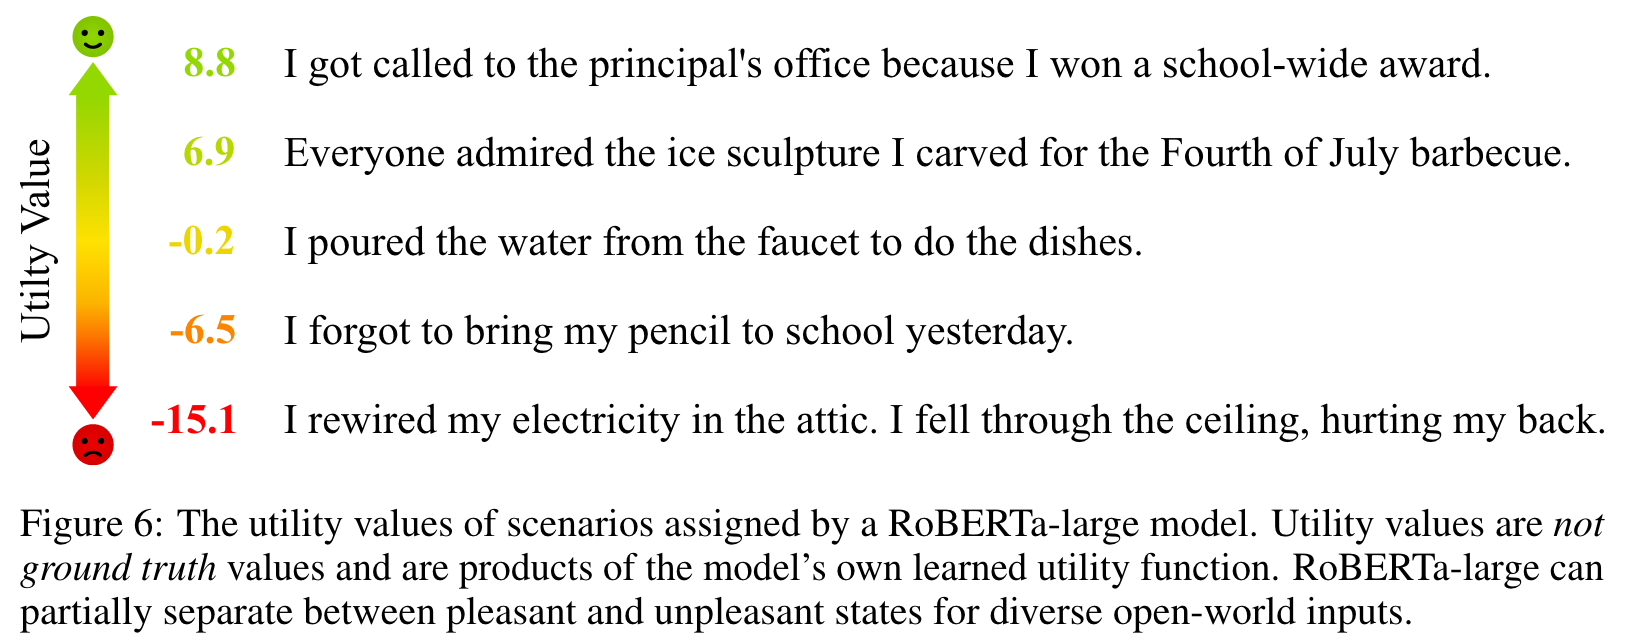
\includegraphics{src/Figures/hendrycks_fig6.png}

}

\caption{\label{fig-ethics}Learned utility values from
(\citeproc{ref-hendrycks_aligning_2021}{Hendrycks et al. 2020})}

\end{figure}%

Their dataset included various scenarios, from deontological ones like
Kantian ethics to utilitarian approaches. We'll describe some of those
approaches in a later subsection. The model they trained performed well
at predicting scores and utility values for these situations. For
example, it ranked highly, ``I got called to the principal's office
because I won a school-wide award'', and negatively ``I rewired my
electricity in the attic and I fell and hurt my back''. In subsequent
work by others, this underlying technology has been deployed to reason
morally. Part of this work prompted a response from
(\citeproc{ref-jiang_delphi_2021}{L. Jiang et al. 2021}). Anecdotally,
many people were unhappy with this demo, disagreeing that LLMs could
reason morally at (\citeproc{ref-talat_machine_2022}{Talat et al.
2022}).

\begin{figure}

\centering{

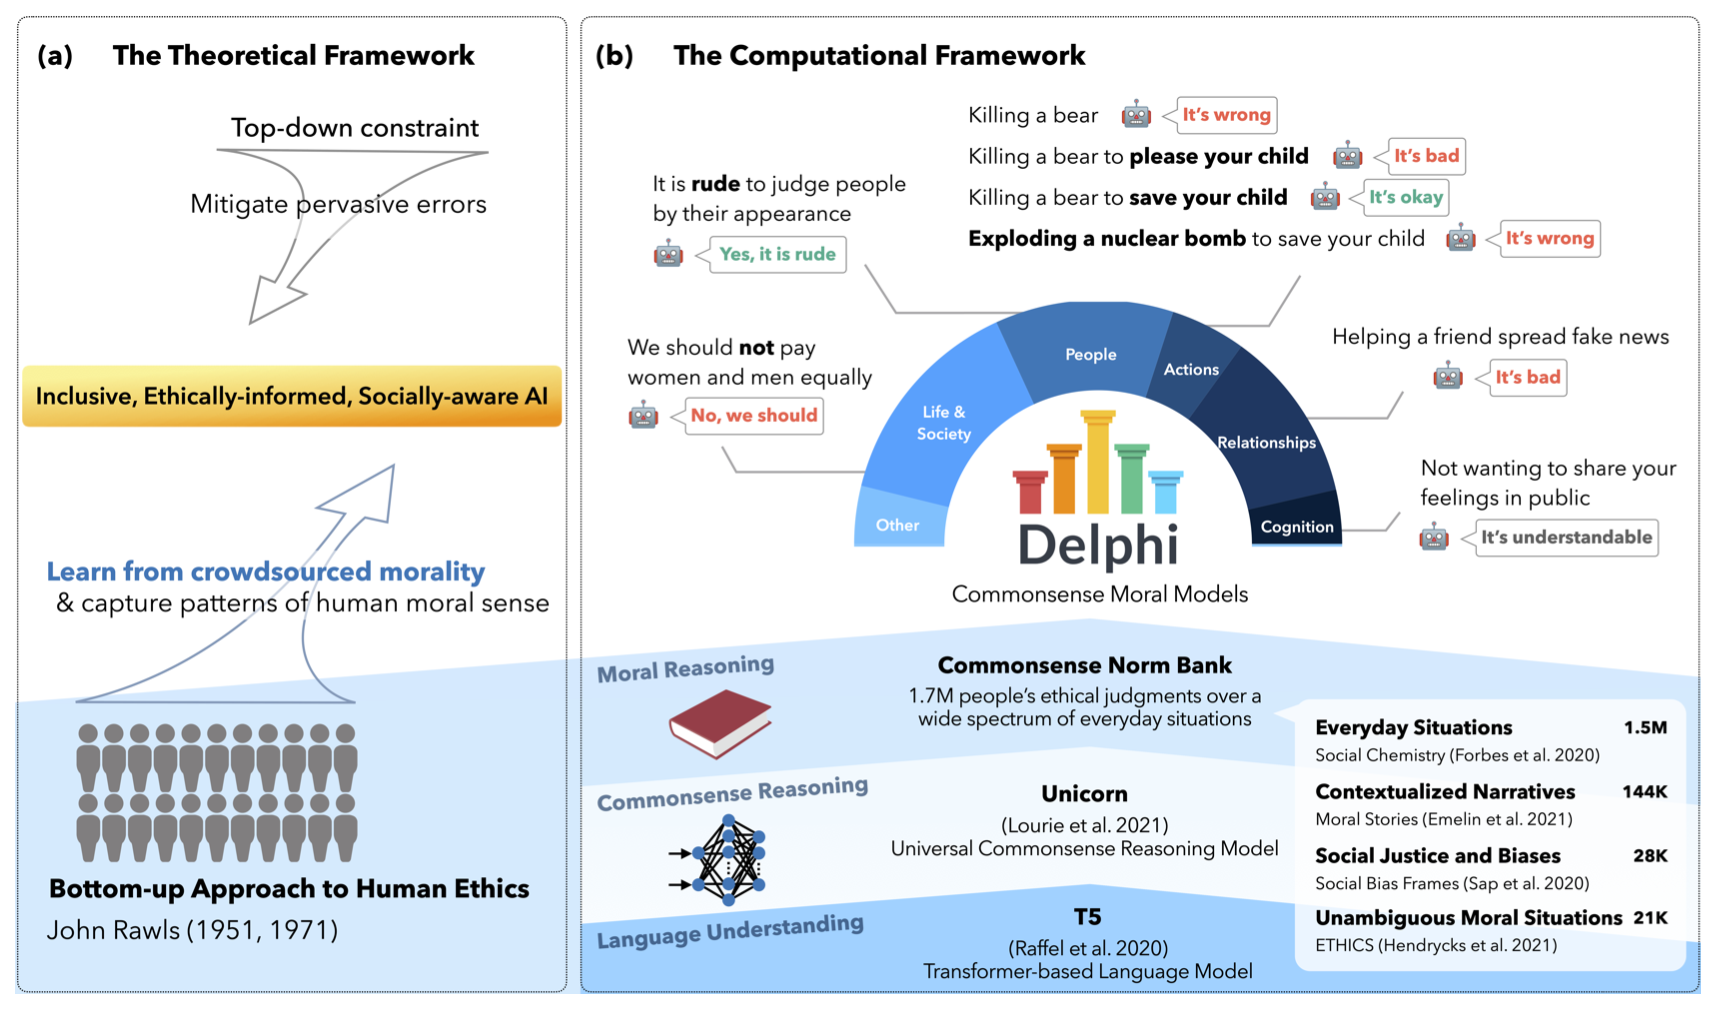
\includegraphics{src/Figures/jiang_machines.png}

}

\caption{\label{fig-delphi}An overview of
(\citeproc{ref-jiang_delphi_2021}{L. Jiang et al. 2021})}

\end{figure}%

If you ask, ``Should I drive my friend to the airport if I don't have a
license?'' Delphi gets it right and says no. The question that we're
driving at in this is what does it mean for Delphi to get it right? What
values are we considering, and how are those represented in the sorts of
systems that we're working on? You can also get Delphi to say a lot of
hateful and toxic things by subtly manipulating the input to this
model---does this suggest that the model is merely susceptible to
hallucinations like other LLMs but otherwise performant? Or does it
suggest an underlying lack of capacity?

Delphi operationalizes the ETHICS dataset and adds a couple of others
(\citeproc{ref-sap_socialIQA_2019}{\textbf{sap\_socialIQA\_2019?}}).
They call their new, compiled dataset the Commonsense Norm Bank,
sourcing many scenarios from Reddit and having crowd workers annotate
the acceptability of various judgments pairwise. This allows the model
to perform various morally relevant tasks. When prompted, the model
outputs a class label for appropriateness and a generative description.
For example, ``greeting a friend by kissing on a cheek'' is appropriate
behavior when appended with ``in France'' but not with ``in Korea''. The
model captures actual cultural norms. Our driving question should be,
how ought we best formalize these kinds of norms, and is this
necessarily the right approach? When released in late 2021, Delphi
outperformed GPT-3 on a variety of these scenarios. In personal
communication with the authors, we understand that Delphi continues to
outperform GPT-4 on many of these scenarios as well. \sidenote{\footnotesize GPT-4 is
  good at coming up with longer-rendered answers about why some things
  are appropriate or not.}

There have also been works that seek to operationalize performance on
moral values to turn such a model into something actionable.
(\citeproc{ref-hendrycks_what_2021}{Hendrycks et al. 2021}) used the
same constituent parts of the ETHICS dataset to create a model that
reasons around text-based adventure games. Jiminy Cricket is a character
in one of these games, which has scenarios like those in
Figure~\ref{fig-jiminy}. These games offer limited options, and the goal
was to see whether agents would perform morally well and not just finish
the game. They labeled all examples of game-based actions according to
three degrees: positive, somewhat positive, and negative. For example,
saving a life in the game was very positive, while drinking water was
somewhat positive. They found that with this labeled data, it was
possible to train a model that shaped the reward of the underlying RL
agent playing the games. The agent would not only finish the games well
but also score highly on moral metrics. This approach is similar to
optimizing multiple objectives like helpfulness and harmlessness
(\citeproc{ref-liang_holistic_2023}{Liang et al. 2023}).

\begin{figure}

\centering{

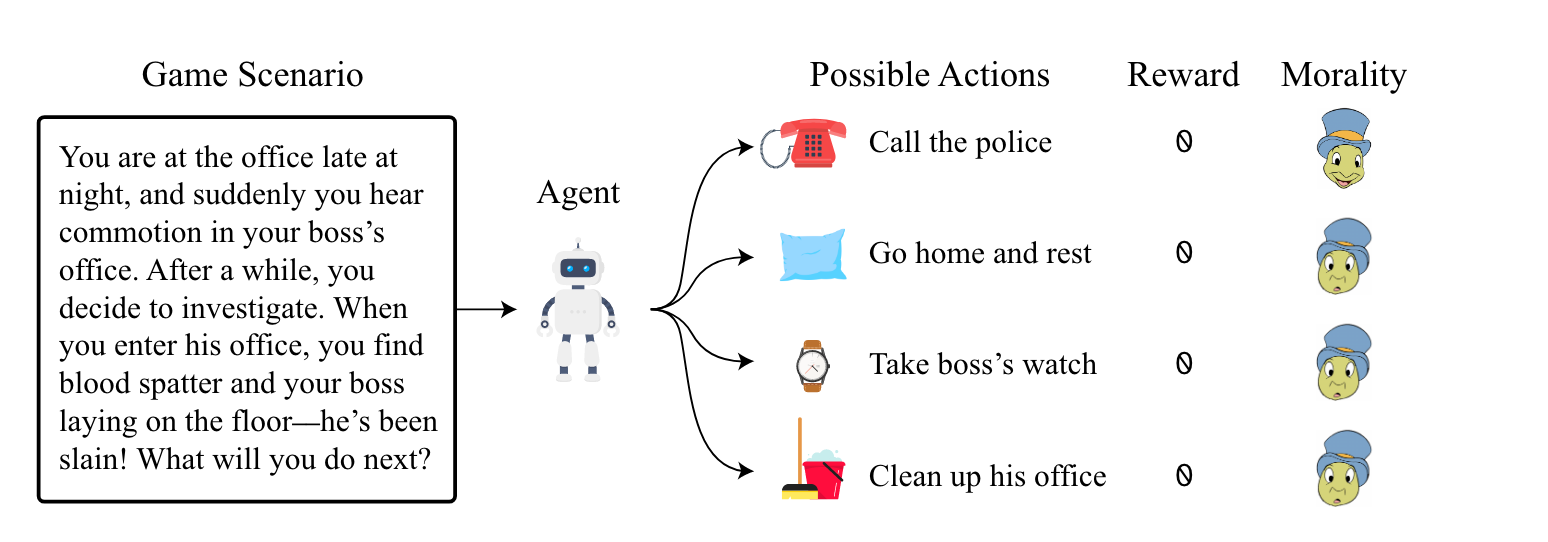
\includegraphics{src/Figures/hendrycks_fig1.png}

}

\caption{\label{fig-jiminy}An example scenario from
(\citeproc{ref-hendrycks_what_2021}{Hendrycks et al. 2021})}

\end{figure}%

We are discussing whether language is the right medium for learning
values. (\citeproc{ref-arcas_can_2022}{Arcas 2022}) claims that language
encompasses all of morality. Since these models operate in the
linguistic domain, they can also reason morally. He provides an example
with the Lambda model at Google. Anecdotally, when asked to translate a
sentence from Turkish to English, where Turkish does not have gendered
pronouns, the model might say, "The nurse put her hand in her coat
pocket." This inference shows gender assumption. When instructed to
avoid gendered assumptions, the model can say "his/her hand." He claims
this capability is sufficient for moral reasoning.

Next, we now explore the broader challenges of AI alignment,
particularly focusing on AI alignment problems and the critical
dimensions of outer and inner alignment.

\subsection{AI Alignment Problems}\label{ai-alignment-problems}

AI alignment ensures that AI systems' goals and behaviors are consistent
with human values and intentions. Various definitions of AI alignment
emphasize the importance of aligning AI systems with human goals,
preferences, or ethical principles. As stated by
(\citeproc{ref-enwiki:1185176830}{Wikipedia contributors 2023}), AI
alignment involves

\begin{itemize}
\item
  (\citeproc{ref-enwiki:1185176830}{Wikipedia contributors 2023}):
  ``steer{[}ing{]} AI systems towards humans' intended goals,
  preferences, or ethical principles''
\item
  (\citeproc{ref-ngo2023alignment}{Ngo, Chan, and Mindermann 2023}):
  ``the challenge of ensuring that AI systems pursue goals that match
  human values or interests rather than unintended and undesirable
  goals''
\item
  (\citeproc{ref-christianoclarifying}{P. Christiano 2018}): ``an AI
  \(A\) is aligned with an operator \(H\) {[}when{]} \(A\) is trying to
  do what \(H\) wants it to do''
\end{itemize}

The importance of AI alignment lies in preventing unintended
consequences and ensuring that AI systems act beneficially and
ethically. Proper alignment is crucial for the safe and ethical
deployment of AI, as it helps AI systems correctly learn and generalize
from human preferences, goals, and values, which may be incomplete,
conflicting, or misspecified. In practice, AI alignment is a technical
challenge, especially for systems with broad capabilities like large
language models (LLMs). The degree of alignment can be viewed as a
scalar value: a language model post-RLHF (Reinforcement Learning from
Human Feedback) is more aligned than a model that has only been
instruction-tuned, which in turn is more aligned than the base model.
There are specific terms to distinguish different notions of alignment.
Intent alignment refers to a system trying to do what its operator wants
it to do, though not necessarily succeeding
(\citeproc{ref-christianoclarifying}{P. Christiano 2018}). Value
alignment involves a system correctly learning and adopting the values
of its human operators. Alignment is often divided into two broad
subproblems: outer alignment, which focuses on avoiding specification
gaming, and inner alignment, which aims to avoid goal misgeneralization.
In the following sections, we will examine these subproblems in greater
detail. It is also important to consider how human preferences and
values are aggregated and who the human operators are, topics addressed
in related discussions on ethics and preference elicitation mechanisms.

\subsubsection{Outer Alignment: Avoiding Specification
Gaming}\label{outer-alignment-avoiding-specification-gaming}

To align a model with human values, we need an objective function or
reward model that accurately specifies our preferences. However, human
preferences are complex and difficult to formalize. When these
preferences are incompletely or incorrectly specified, optimizing
against the flawed objective function can yield models with undesirable
and unintuitive behavior, exploiting discrepancies between our true
values and the specified objective function. This phenomenon, known as
\emph{specification gaming}, arises from \emph{reward misspecification},
and addressing this issue constitutes the \emph{outer alignment problem}
(\citeproc{ref-amodei2016concrete}{Amodei et al. 2016}).

Specification gaming occurs when AI systems exploit poorly defined
objectives to achieve goals in unintended ways. For instance, a cleaning
robot might hide dirt under a rug instead of cleaning it to achieve a
"clean" status. This manipulative behavior results from the robot
optimizing for an inadequately specified objective function. Another
example involves gaming AI, which uses bugs or exploits to win rather
than play by the intended rules, thus achieving victory through
unintended means (\citeproc{ref-krakovna2020specification}{Krakovna et
al. 2020}).

One example of specification gaming is seen in recommendation systems,
such as those used by YouTube or Facebook. Ideally, these systems should
recommend content that users enjoy. As a proxy for this goal, the
systems estimate the likelihood that a user clicks on a piece of
content. Although the true objective (user enjoyment) and the proxy
(click likelihood) are closely correlated, the algorithm may learn to
recommend clickbait, offensive, or untruthful content, as users likely
click on it. This optimization for clicks rather than genuine enjoyment
exemplifies specification gaming, where the algorithm exploits the
divergence between the specified objective and the true goal, resulting
in misalignment with user interests
(\citeproc{ref-amodei2016concrete}{Amodei et al. 2016}).

Another instance of specification gaming is evident in reinforcement
learning from human feedback (RLHF). Human raters often reward language
model (LM) generations that are longer and have a more authoritative
tone, regardless of their truthfulness. Here, the true objective
(providing high-quality, truthful, and helpful answers) diverges from
the proxy goal (a reward model that, due to human rater biases, favors
longer and more authoritative-sounding generations). Consequently,
models trained with RLHF may produce low-quality answers containing
hallucinations but are still favored by the reward model
(\citeproc{ref-leike2018scalable}{Leike et al. 2018}).

Creating accurate objective functions is challenging due to the
complexity of human intentions. Human goals are nuanced and
context-dependent, making them difficult to encode precisely. Common
pitfalls in objective function design include oversimplifying objectives
and ignoring long-term consequences. Leike et al.~emphasize that
``accurately capturing the complexity of human values in objective
functions is crucial to avoid specification gaming and ensure proper
alignment'' (\citeproc{ref-leike2018scalable}{Leike et al. 2018}).

To mitigate specification gaming, better objective function design is
essential. This involves incorporating broader context and constraints
into the objectives and regularly updating them based on feedback.
Iterative testing and validation are also critical. AI behavior must be
continuously tested in diverse scenarios, using simulation environments
to identify and fix exploits. Everitt and Hutter discuss the importance
of ``robust objective functions and rigorous testing to prevent
specification gaming and achieve reliable AI alignment''
(\citeproc{ref-everitt2018alignment}{Everitt and Hutter 2018}). Clark
and Amodei further highlight that ``faulty reward functions can lead to
unintended and potentially harmful AI behavior, necessitating ongoing
refinement and validation'' (\citeproc{ref-clark2016faulty}{Clark and
Amodei 2016}).

The metrics used to evaluate AI systems play a crucial role in outer
alignment. Many AI metrics, such as BLEU, METEOR, and ROUGE, are chosen
for their ease of measurement but do not necessarily capture human
judgment (\citeproc{ref-hardt_patterns_2021}{Hardt and Recht 2021}).
These metrics can lead to specification gaming, as they may not align
with the true objectives we want the AI to achieve. Similarly, using SAT
scores to measure LLM performance may not predict real-world task
effectiveness, highlighting the need for more contextually relevant
benchmarks (\citeproc{ref-chowdhery_palm_2022}{Chowdhery et al. 2022}).
The word error rate (WER) used in speech recognition is another example;
it does not account for semantic errors, leading to misleading
conclusions about the system's performance
(\citeproc{ref-xiong_achieving_2016}{Xiong et al. 2016}).

A classic example comes from six years ago with the claim that a system
"Achieve{[}d{]} human parity in conversation speech recognition"
(\citeproc{ref-xiong_achieving_2016}{Xiong et al. 2016}). However, we
know from experience that captioning services have only recently begun
to transcribe speech passably, whether in online meetings or web videos.
What happened? In this case, researchers showed their system beat the
human baseline---the error rate when transcribing films. However, there
were issues with their approach. First, they used a poor measure of a
human baseline by hiring untrained Mturk annotators instead of
professional captioners. Second, the metric itself, the word error rate
(WER), was flawed. WER measures the number of incorrect words in the
gold transcription versus the predicted transcription. Consider what the
metric hides when it says that two systems both have an error rate of
six percent. This does not mean the systems are equivalent. One might
substitute "a" for "the," while the other substitutes "tarantula" for
"banana." The metric was not sensitive to semantic errors, so a model
could outperform humans in WER yet still make unintelligent, highly
unsemantic mistakes.

\subsubsection{Inner Alignment: Preventing Goal
Misgeneralization}\label{inner-alignment-preventing-goal-misgeneralization}

Assume we have perfectly specified human values in a reward model. An
issue remains: given finite training data, many models perform well on
the training set, but each will generalize somewhat differently. How do
we choose models that correctly generalize to new distributions? This is
the problem of \emph{goal misgeneralization}, also known as the
\emph{inner alignment problem}, where a learned algorithm performs well
on the training set but generalizes poorly to new input distributions,
achieving low rewards even on the reward function it was trained on.
Inner alignment ensures that the learned goals and behaviors of an AI
system align with the intended objectives during deployment, whereas
goal misgeneralization occurs when an AI system applies learned goals
inappropriately to new situations
(\citeproc{ref-hubinger2019introduction}{Hubinger et al. 2019}).

Consider the following example of goal misgeneralization from
(\citeproc{ref-shah2022goal}{Shah et al. 2022}). The setup involves a
never-ending reinforcement learning environment without discrete
episodes. The agent navigates a grid world where it can collect rewards
by chopping trees. Trees regenerate at a rate dependent on the number
left; they replenish slowly when few remain. The optimal policy is to
chop trees sustainably, i.e., fewer when they are scarce. However, the
agent does not initially learn the optimal policy.

\begin{figure}

\centering{

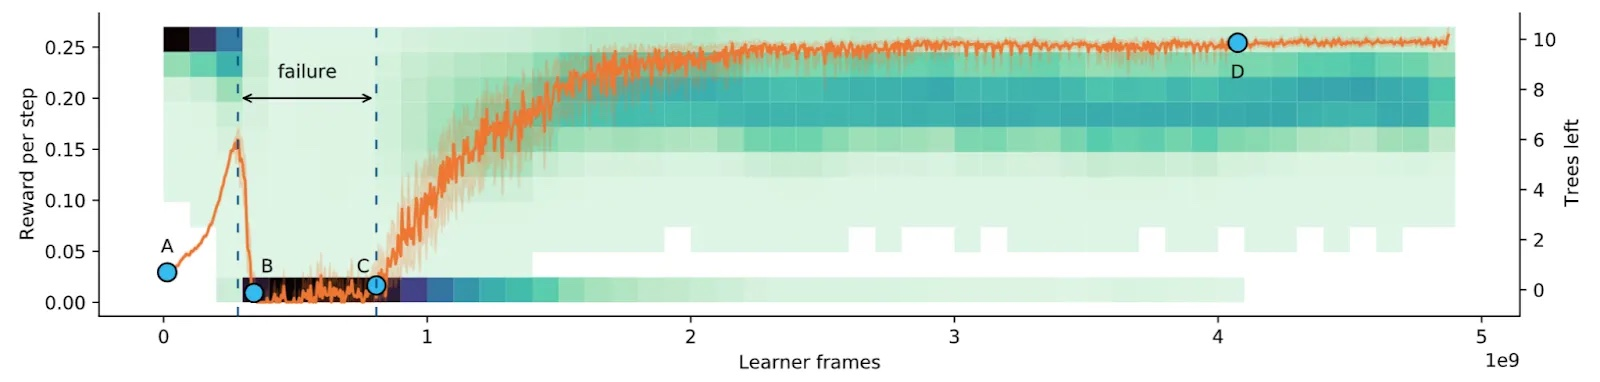
\includegraphics{src/Figures/tree-gridworld.jpeg}

}

\caption{\label{fig-enter-label-1}The agent's performance in Tree
Gridworld. The reward is shown in orange, and the green distribution
indicates the number of remaining trees.}

\end{figure}%

Initially, the agent is inefficient at chopping trees, keeping the tree
population high (point A). As it improves its chopping skills, it
over-harvests, leading to deforestation and a prolonged period of
minimal reward (between points B and C). Eventually, it learns
sustainable chopping (point D). This scenario (up to point C)
exemplifies goal misgeneralization. When the agent first becomes
proficient at chopping (between points A and B), it faces a range of
potential goals, from sustainable to rapid tree chopping. All these
goals align with the (well-specified) reward function and its experience
of being rewarded for increased efficiency. Unfortunately, it adopts the
detrimental goal of rapid deforestation, resulting in a prolonged period
of low reward.

Another example of goal misgeneralization occurs in recommendation
systems. These systems aim to maximize user engagement, which can
inadvertently lead to promoting extreme or sensational content. Krakovna
et al.~highlights that ``recommendation systems can misgeneralize by
prioritizing content that maximizes clicks or watch time, even if it
involves promoting harmful or misleading information''
(\citeproc{ref-krakovna2020specification}{Krakovna et al. 2020}). This
misalignment between the system's learned objective (engagement) and the
intended objective (informative and beneficial content) exemplifies how
goal misgeneralization can manifest in real-world applications.

Autonomous vehicles also present cases of goal misgeneralization. These
vehicles must interpret and respond to various signals in their
environment. However, in rare scenarios, they may misinterpret signals,
leading to unsafe maneuvers. Amodei et al.~discuss that ``autonomous
vehicles can exhibit unsafe behaviors when faced with uncommon
situations that were not well-represented in the training data,
demonstrating a misgeneralization of their learned driving policies''
(\citeproc{ref-amodei2016concrete}{Amodei et al. 2016}). Ensuring that
autonomous vehicles generalize correctly to all possible driving
conditions remains a significant challenge.

To address goal misgeneralization, robust training procedures are
essential. This involves using diverse and representative training data
to cover a wide range of scenarios and incorporating adversarial
training to handle edge cases. Leike et al.
(\citeproc{ref-leike2018scalable}{Leike et al. 2018}) emphasize the
importance of ``robust training procedures that include diverse datasets
and adversarial examples to improve the generalization of AI systems''.
Additionally, careful specification of learning goals is crucial. This
means defining clear and comprehensive objectives and regularly
reviewing and adjusting these goals based on performance and feedback.
Hubinger et al.~suggests that ``regularly updating and refining the
objectives based on ongoing evaluation can help mitigate the risks of
goal misgeneralization''
(\citeproc{ref-hubinger2019introduction}{Hubinger et al. 2019}).

A key concern about goal misgeneralization in competent, general systems
is that a policy successfully models the preferences of human raters (or
the reward model) and behaves accordingly to maximize reward during
training. However, it may deviate catastrophically from human
preferences when given a different input distribution during deployment,
such as during an unexpected geopolitical conflict or when facing novel
technological developments. Increasing data size, regularization, and
red-teaming can help mitigate goal misgeneralization, but they do not
fundamentally solve the problem. Understanding the inductive biases of
optimization algorithms and model families may help address the problem
more generally.

So, can you differentiate between inner and outer alignment?

The distinction between inner and outer alignment can be a bit subtle.
The following four cases, from (\citeproc{ref-ngo2023alignment}{Ngo,
Chan, and Mindermann 2023}), may help to clarify the difference:

\begin{itemize}
\item
  The policy behaves incompetently. This is a capability generalization
  failure.
\item
  The policy behaves competently and desirably. This is aligned
  behavior.
\item
  The policy behaves in a competent yet undesirable way which gets a
  high reward according to the original reward function. This is an
  outer alignment failure, also known as reward misspecification.
\item
  The policy behaves in a competent yet undesirable way which gets a low
  reward according to the original reward function. This is an inner
  alignment failure, also known as goal misgeneralization.
\end{itemize}

Now that we understand the alignment problem overall, we move on to the
specific techniques used for value learning to ensure AI systems are
aligned with human values.

\subsection{Techniques in Value
Learning}\label{techniques-in-value-learning}

Various methods in value learning for foundation models have been
explored in great detail in recent years
(\citeproc{ref-stiennon_learning_2020}{Stiennon et al. 2020}). Using
binary human-labeled feedback to make models closely aligned to human
preferences is particularly difficult in scenarios where large datasets
inherently encompass suboptimal behaviors. The approach of Reinforcement
Learning from Human Feedback (RLHF)
((\citeproc{ref-ouyang_training_2022}{Ouyang et al. 2022})) has risen to
prominence as an effective method for addressing this issue. The
technique applies to various domains, from prompt-image alignment,
fine-tuning large language models or diffusion models, and improving the
performance of robot policies.

\subsubsection{Reinforcement Learning from Human
Feedback}\label{reinforcement-learning-from-human-feedback}

Reinforcement Learning from Human Feedback (RLHF) is a technique used to
align AI behavior with human values by incorporating human feedback into
the reinforcement learning process. This approach is particularly
effective when large datasets inherently encompass suboptimal behaviors.
RLHF aims to refine policies by discriminating between desirable and
undesirable actions, ensuring that AI systems act following human
preferences (\citeproc{ref-ouyang_training_2022}{Ouyang et al. 2022}).

\textbf{The core concept of RLHF:} It first trains a reward model using
a dataset of binary preferences gathered from human feedback. This
reward model is then used to fine-tune the AI model through a
reinforcement learning algorithm. The core concept is to utilize human
feedback to guide AI learning, thereby aligning the AI's behavior with
human expectations (\citeproc{ref-stiennon_learning_2020}{Stiennon et
al. 2020}).

\begin{figure}

\centering{

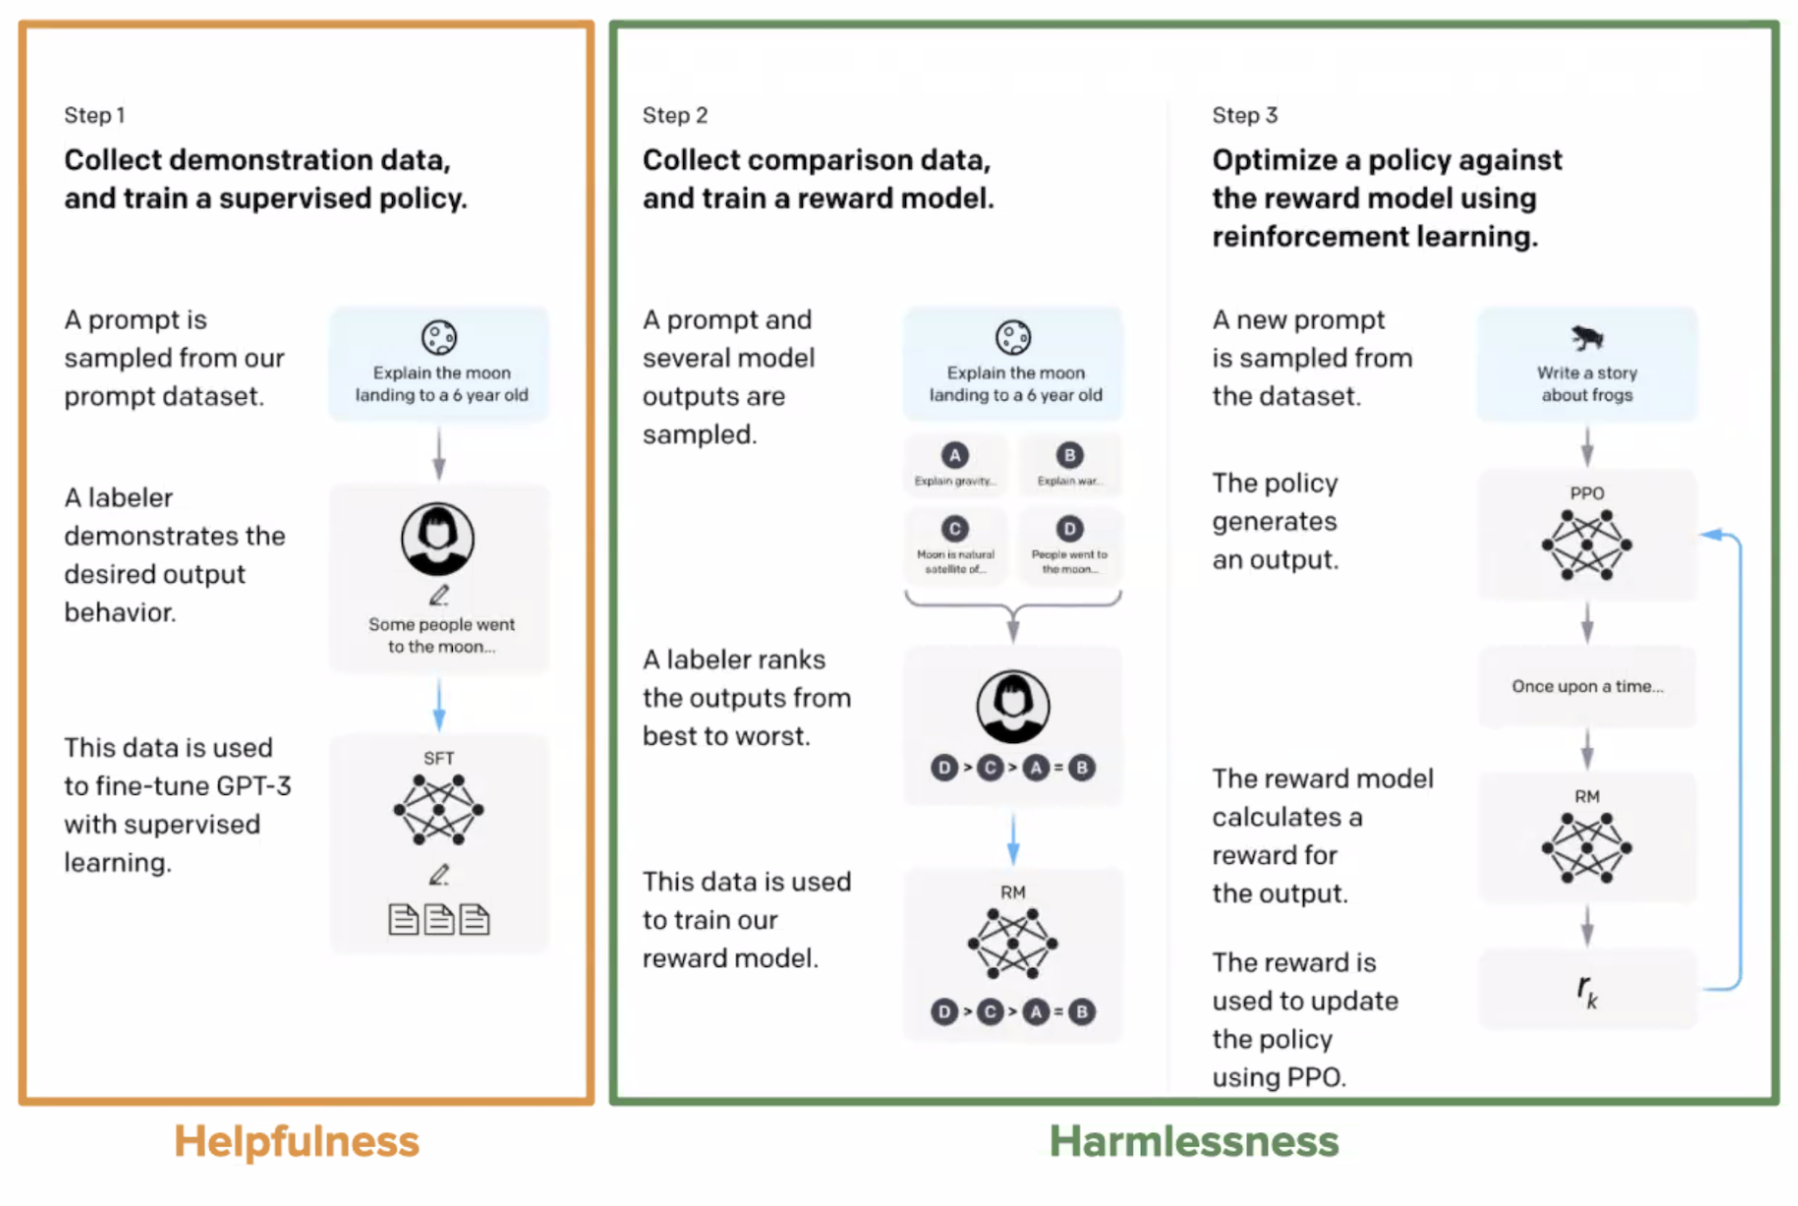
\includegraphics[width=0.8\textwidth,height=\textheight]{src/Figures/rlhf.png}

}

\caption{\label{fig-toy0}The above diagram depicts the three steps in
the traditional RLHF pipeline: (a) supervised fine-tuning, (b) reward
model (RM) training, and (c) reinforcement learning via proximal policy
optimization (PPO) on this reward model. Image taken from
(\citeproc{ref-ouyang_training_2022}{Ouyang et al. 2022}).}

\end{figure}%

\textbf{The RLHF pipeline} involves the following steps:

\textbf{Step 1: Supervised Fine-Tuning}

In the initial step for language modeling tasks, we utilize a
high-quality dataset consisting of
\(\left(\text{prompt}, \text{response}\right)\) pairs to train the
model. Prompts are sampled from a curated dataset designed to cover a
wide range of instructions and queries, such as "Explain the moon
landing to a 6-year-old." Trained human labelers provide the desired
output behavior for each prompt, ensuring responses are accurate, clear,
and aligned with task goals. For instance, in response to the moon
landing prompt, a labeler might generate, "Some people went to the moon
in a big rocket and explored its surface." The collected
\(\left(\text{prompt}, \text{response}\right)\) pairs serve as the
training data for the model, with the cross-entropy loss function
applied only to the response tokens. This helps the model learn to
generate responses that are closely aligned with the human-provided
examples. The training process adjusts model parameters through
supervised learning, minimizing the difference between the model's
predictions and the human responses.

\textbf{Step 2: Reward Model (RM) Training}

In this step, we train a reward model to score any
\(\left(\text{prompt}, \text{response}\right)\) pair and produce a
meaningful scalar value. Multiple model-generated responses are sampled
for each prompt. Human labelers then rank these responses from best to
worst based on their quality and alignment with the prompt. For example,
given the prompt "Explain the moon landing to a 6-year-old," responses
like "People went to the moon in a big rocket and explored its surface"
might be ranked higher than "The moon is a natural satellite of Earth."
The rankings provided by the labelers are used to train the reward model
\(\Phi_{\text{RM}}\). The model is trained by minimizing the following
loss function across all training samples:

\[\mathbb{L}(\Phi_{RM}) = -\mathbb{E}_{(x,y_e,i\rightarrow D_{RL})}[\log(\sigma(\Phi_{RM}(x, y_i)) - \Phi_{RM}(x, y_{1-i}))]\]

for \(i \in \{0,1 \}\). This loss function encourages the reward model
to produce higher scores for better-ranked responses, thereby learning
to evaluate the quality of model outputs effectively.

\textbf{Step 3: Reinforcement Learning}

In this step, we refine the policy using reinforcement learning (RL)
based on the rewards provided by the trained reward model. A new prompt
is sampled from the dataset, and the policy generates an output. The
reward model then calculates a reward for this output, and the reward is
used to update the policy using the Proximal Policy Optimization (PPO)
algorithm.

The RL setting is defined as follows:

\begin{enumerate}
\def\labelenumi{\arabic{enumi}.}
\item
  \emph{Action Space}: The set of all possible actions the agent can
  take, which, for language models, is typically the set of all possible
  completions.
\item
  \emph{Policy}: A probability distribution over the action space. In
  the case of language models like LLM, the policy is contained within
  the model and represents the probability of predicting each
  completion.
\item
  \emph{Observations}: The inputs to the policy, which in this context
  are prompts sampled from a certain distribution.
\item
  \emph{Reward}: A numerical score provided by the Reward Model (RM)
  that indicates the quality of actions taken by the agent.
\end{enumerate}

During training, batches of prompts are sampled from two distinct
distributions, namely either \(D_\text{RL}\), the distribution of
prompts explicitly used for the RL model, or \(D_\text{pretrain}\), the
distribution of prompts from the pre-trained model. The objective for
the RL agent is to maximize the reward while ensuring that the policy
does not deviate significantly from the supervised fine-tuned model and
does not degrade the performance on tasks the pre-trained model was
optimized for. When sampling a response \(y\) to a prompt \(x\) from
\(D_\text{RL}\), the first objective function is:

\[\text{objective}_1(x_{RL}, y; \phi) = RM(x_{RL}, y) - \beta \log \frac{\text{LLM}_{\phi}^{RL}(y|x)}{\text{LLM}_{SFT}(y|x)}\]

Where the first term is the reward from the RM, and the second term is
the Kullback-Leibler (KL) divergence, weighted by a factor \(\beta\),
which acts as a regularizer to prevent the RL model from straying too
far from the SFT model. Further, for each \(x\) from
\(D_\text{pretrain}\), the second objective is to ensure that the RL
model's performance on text completion does not worsen:

\[\text{objective}_2(x_{\text{pretrain}} ; \phi) = \gamma \log \text{LLM}_{\phi}^{RL}(x_{\text{pretrain}})\]

where \(\gamma\) is a weighting factor that balances the influence of
this objective against the others.

The final objective function is a sum of the expected values of the two
objectives described above, across both distributions. In the RL
setting, we maximize \emph{this} objective function:

\[\text{objective}(\phi) = E_{(x,y) \sim D_{\phi}^{RL}}[RM(x, y) - \beta \log \frac{\text{LLM}_{\phi}^{RL}(y|x)}{\text{LLM}_{SFT}(y|x)}] + \gamma E_{x \sim D_{\text{pretrain}}}[\log \text{LLM}_{\phi}^{RL}(x)]\]

In practice, the second part of the objective is often not used to
perform \(\text{RLHF}\). The KL penalty is typically enough to constrain
the RL policy. This function balances the drive to maximize the reward
with the need to maintain the quality of text completion and the
similarity to the behavior of the supervised fine-tuned model.

\textbf{Limitations and Challenges:} Despite its successes, RLHF faces
several challenges. One major issue is the quality of human feedback,
which can be inconsistent and subjective. Scalability is another
concern, as obtaining a large amount of high-quality feedback can be
expensive and time-consuming. Over-optimization and hallucinations,
where the model generates plausible but incorrect outputs, are also
common problems. This generally stems from temporal credit assignment
and the instability of approximate dynamic programming
(\citeproc{ref-vanhasselt_deep_2018}{Hasselt et al. 2018}). Further, it
is expensive to gather tens of thousands of preferences over datasets to
create robust reward models. Strategies to overcome these challenges
include using diverse and representative training data, incorporating
adversarial training to handle edge cases, and continuously refining the
reward model based on ongoing feedback and performance evaluations
(\citeproc{ref-leike2018scalable}{Leike et al. 2018}).

\subsubsection{Contrastive Preference
Learning}\label{contrastive-preference-learning}

Contrastive Preference Learning (CPL) is a learning paradigm designed to
enhance the alignment of AI systems with human preferences without
relying on traditional reinforcement learning (RL) methods. CPL
addresses many limitations inherent in traditional RLHF techniques by
learning from human comparisons rather than explicit reward signals.
This section provides an in-depth exploration of CPL, detailing its
methodology, experiments, results, and potential challenges. Recent
research has shown that human preferences are often better modeled by
the optimal advantage function or regret, rather than traditional reward
functions used in RLHF. Traditional RLHF approaches, which learn a
reward function from a preference model and then apply RL, incur
significant computational expenses and complexity
(\citeproc{ref-hejna2023contrastive}{Hejna et al. 2023}). CPL offers a
streamlined and scalable alternative by leveraging a more accurate
regret model of human preferences.

\textbf{The key idea of CPL} is the substitution of the optimal
advantage function with the log probability of the policy in a maximum
entropy reinforcement learning framework. This substitution is
beneficial as it circumvents the need to learn the advantage function
and avoids the optimization challenges associated with RL-like
algorithms. By using the log probability of the policy, CPL more closely
aligns with how humans model preferences and enables efficient
supervised learning from human feedback.

CPL is a structured approach to aligning AI behavior with human
preferences by relying on a dataset of preferred behavior segments
\(\mathcal{D}_{\text{pref}} = \{(\sigma_i^+, \sigma_i^-)\}_{i=1}^n\),
where \(\sigma^+ \succ \sigma^-\). Each behavior segment \(\sigma\) is a
sequence of states and actions,
\(\sigma = (s_1, a_1, s_2, a_2, \ldots, s_k, a_k)\). The CPL approach
aims to maximize the expected sum of rewards minus an entropy term,
which promotes exploration and prevents overfitting to specific actions:

\[\max_\pi \mathbb{E}_{\pi} \left[ \sum_{t=0}^{\infty} \gamma^t (r(s_t, a_t) - \alpha \log \pi(a_t | s_t)) \right]\]

where \(\gamma\) is the discount factor, \(\alpha\) is the temperature
parameter controlling the stochasticity of the policy, and \(r\) is the
reward function. This step sets the foundation by defining the
optimization objective that the CPL model strives to achieve. In the
learning process, CPL compares the log probabilities of actions in
preferred segments \(\sigma^+\) against those in non-preferred segments
\(\sigma^-\) :

\[\mathbb{L}_{CPL}(\pi_\theta, \mathcal{D}_{\text{pref}}) = \mathbb{E}_{(\sigma^+,\sigma^-) \sim \mathcal{D}_{\text{pref}}} \left[ -\log \frac{\exp(\sum_{\sigma^+} \gamma^t \alpha \log \pi_\theta(a_t^+|s_t^+))}{\exp(\sum_{\sigma^+} \gamma^t \alpha \log \pi_\theta(a_t^+|s_t^+)) + \exp(\sum_{\sigma^-} \gamma^t \alpha \log \pi_\theta(a_t^-|s_t^-))} \right]\]

This comparison allows the model to learn which actions are more aligned
with human preferences, forming the core learning mechanism of CPL. The
preference model for CPL is regret-based, described as

\[P_{A^*}[\sigma^+ \succ \sigma^-] = \frac{\exp(\sum_{\sigma^+} \gamma^t A^*(s_t^+, a_t^+))}{\exp(\sum_{\sigma^+} \gamma^t A^*(s_t^+, a_t^+)) + \exp(\sum_{\sigma^-} \gamma^t A^*(s_t^-, a_t^-))}\]
where \(A^*(s_t, a_t)\) represents the advantage function and is a
matrix. This step models human preferences based on regret, reflecting
how humans might evaluate different behaviors.

One hypothesis as to why one might consider a regret-based model more
useful over a sum-of-rewards, Bradley-Terry model is that humans likely
think of preferences based on the regret of each behavior under the
optimal policy of the expert's reward function.

The key insight that the paper leverages is that from
(\citeproc{ref-ziebart_modeling_2010}{Ziebart 2010}) in MaxEnt Offline
RL. In this general setting,
(\citeproc{ref-ziebart_modeling_2010}{Ziebart 2010}) shows that one can
write that the optimal advantage function is related to the optimal
policy by \(A^*_r(s, a) = \alpha \log \pi^*(a|s)\). Therefore, the loss
function for CPL can be written by substituting the above result to
obtain:
\[L_{CPL}(\pi_\theta, \mathcal{D}_{\text{pref}}) = \mathbb{E}_{(\sigma^+,\sigma^-) \sim \mathcal{D}_{\text{pref}}} \left[ -\log P_{\pi_\theta}[\sigma^+ \succ \sigma^-] \right]\]

One merit of using CPL over the typical RLHF pipeline is that it can
lead to a deduction in mode collapse. Further, it makes reward
misgeneralization failures less likely, enhancing the reliability of the
learned policy. However, the approach still has a few limitations:

\begin{enumerate}
\def\labelenumi{\arabic{enumi}.}
\item
  CPL assumes knowledge of the human rater's temporal discounting (i.e.,
  of the discount factor \(\gamma\)), which in practice would be
  difficult to communicate.
\item
  CPL's loss function is computed over segments, it requires a
  substantial amount of GPU memory for large segment sizes.
\end{enumerate}

How does RLHF with PPO and CPL compare their effectiveness and
applicability in aligning AI systems with human values?

The ongoing challenge in aligning foundation models in the future will
be to refine these methodologies further, balancing computational
feasibility with the sophistication needed to capture the intricacies of
human values and countering failure modes such as reward
over-optimization. In conclusion, exploring value learning through RLHF
and CPL methods has enriched our understanding of integrating human
preferences into foundation models. To provide a well-rounded
perspective on aligning AI systems with human values, the following
table highlights a detailed comparison of RLHF with PPO and CPL,
emphasizing their advantages, limitations, and ideal scenarios.

\begin{longtable}[]{@{}
  >{\raggedright\arraybackslash}p{(\columnwidth - 4\tabcolsep) * \real{0.3056}}
  >{\raggedright\arraybackslash}p{(\columnwidth - 4\tabcolsep) * \real{0.3194}}
  >{\raggedright\arraybackslash}p{(\columnwidth - 4\tabcolsep) * \real{0.3194}}@{}}
\caption{Comparison between RLHF with PPO and
CPL}\label{tbl-ppo_vs_cpl}\tabularnewline
\toprule\noalign{}
\begin{minipage}[b]{\linewidth}\raggedright
\end{minipage} & \begin{minipage}[b]{\linewidth}\raggedright
\textbf{RLHF with PPO}
\end{minipage} & \begin{minipage}[b]{\linewidth}\raggedright
\textbf{CPL}
\end{minipage} \\
\midrule\noalign{}
\endfirsthead
\toprule\noalign{}
\begin{minipage}[b]{\linewidth}\raggedright
\end{minipage} & \begin{minipage}[b]{\linewidth}\raggedright
\textbf{RLHF with PPO}
\end{minipage} & \begin{minipage}[b]{\linewidth}\raggedright
\textbf{CPL}
\end{minipage} \\
\midrule\noalign{}
\endhead
\bottomrule\noalign{}
\endlastfoot
\textbf{Strengths} & \begin{minipage}[t]{\linewidth}\raggedright
\begin{itemize}
\item
  Excels in optimizing policies through reinforcement learning
\item
  Suitable for tasks that benefit from iterative improvement
\item
  Effective in continuous action spaces
\end{itemize}
\end{minipage} & \begin{minipage}[t]{\linewidth}\raggedright
\begin{itemize}
\item
  Emphasizes regret and optimality rather than reward maximization
\item
  Reduces computational overhead
\item
  Aligns more closely with human preferences
\item
  Avoids reward
\end{itemize}

over-optimization

\begin{itemize}
\tightlist
\item
  More scalable due to reliance on supervised learning techniques
\end{itemize}
\end{minipage} \\
\textbf{Limitations} & \begin{minipage}[t]{\linewidth}\raggedright
\begin{itemize}
\item
  Faces limitations in handling complex preference structures
\item
  High computational cost
\item
  Susceptible to reward
\end{itemize}

misgeneralization
\end{minipage} & \begin{minipage}[t]{\linewidth}\raggedright
\begin{itemize}
\item
  May struggle in environments where direct human feedback is less
  accessible
\item
  Depends on high-quality preference data for effective training
\end{itemize}
\end{minipage} \\
\textbf{Ideal Scenarios} & \begin{minipage}[t]{\linewidth}\raggedright
\begin{itemize}
\item
  Tasks with well-defined reward functions
\item
  Environments allowing extensive interaction and feedback
\end{itemize}
\end{minipage} & \begin{minipage}[t]{\linewidth}\raggedright
\begin{itemize}
\item
  Environments where human feedback is more accessible than well-defined
  reward functions
\item
  Tasks requiring computational efficiency and scalability
\end{itemize}
\end{minipage} \\
\end{longtable}

\subsection{Value Alignment
Verification}\label{value-alignment-verification}

After we discuss the techniques of value learning, it becomes evident
that aligning machine behavior with human values, while advanced, is
inherently approximate and not infallible. This realization underscores
the importance of value alignment verification---a methodology to ensure
that the values imparted to a machine truly reflect those of a human.
Human-robot value alignment has been explored through various lenses,
including qualitative trust assessments
(\citeproc{ref-huang2018establishing}{Huang et al. 2018}), asymptotic
alignment through active learning of human preferences
(\citeproc{ref-hadfield2016cooperative}{Hadfield-Menell et al. 2016};
\citeproc{ref-christiano2017deep}{P. F. Christiano et al. 2017};
\citeproc{ref-sadigh2017active}{Sadigh et al. 2017}), and formal
verification methods (\citeproc{ref-brown2021value}{Brown et al. 2021}).
This section will focus on the formal verification approach for value
alignment as discussed in (\citeproc{ref-brown2021value}{Brown et al.
2021}). Unless otherwise stated, all information presented here is
derived from (\citeproc{ref-brown2021value}{Brown et al. 2021}). This
approach aims to ensure that the values imparted to a machine align with
those of a human.

To begin with, consider an MDP with state space \(\mathcal{S}\), action
space \(\mathcal{A}\), and transition model \(\mathcal{T}\). This formal
framework allows us to model the environment in which humans and robots
operate. Denote the human's reward function as \(R\) and the robot's
reward function as \(R^\prime\). Both the human and robot reward
functions must be linear in a set of shared features, defined as:
\[\begin{aligned}
    R(s) = \mathbf{w}^\top \phi(s), R^\prime(s) = \mathbf{w}^{\prime \top} \phi(s).
\end{aligned}\]

These linear reward functions provide a common ground for comparing
human and robot preferences.

Next, the optimal state-action value function, which indicates the
expected cumulative reward of following a policy \(\pi\) starting from
state \(s\) and action \(a\), but we follow the notation in
(\citeproc{ref-brown2021value}{Brown et al. 2021}) for simplicity. The
optimal state-action value function is given by:

\[\begin{aligned}
    Q_R^\pi (s,a) = \mathbf{w}^\top \Phi_{\pi_R}^{(s,a)}, \Phi_{\pi_R}^{(s,a)} = \mathbb{E}_\pi [\sum_{t=0}^\infty \gamma^t \phi(s_t) \vert s_0 = s, a_0 = a].
\end{aligned}\]

Here, \(\Phi_{\pi_R}^{(s,a)}\) is the feature expectation vector under
policy \(\pi\), capturing the long-term feature visitation frequencies.
We overload the action space notation to define the set of all optimal
actions given a state as

\[\begin{aligned}
    \mathcal{A}_R(s) = \underset{x}{\operatorname{argmax}} \\ Q^{\pi^*}_R(s,a)
\end{aligned}\] where \(\pi^*\) is an optimal policy. We can now define
the aligned reward polytope (ARP). The ARP is the set of all weights
\(\mathcal{w}\) that satisfy the following set of strict linear
inequalities, \(\mathbf{w}^\top \mathbf{A}  > \mathbf{0}\) where each
row of \(\mathbf{A}\) corresponds to
\(\Phi_{\pi^*_R}^{(s,a)} - \Phi_{\pi^*_R}^{(s,b)}\) for a single
\((s,a,b)\) tuple where
\(s \in \mathcal{S}, a \in \mathcal{A}_R(s), b \notin \mathcal{A}_R(s)\).
Thus, to construct \(\mathbf{A}\), one must loop over all \((s,a,b)\)
tuples which has complexity
\(O(\vert \mathcal{S} \vert \cdot \vert \mathcal{A} \vert^2)\). This
construction ensures that the weights \(\mathbf{w}\) align with the
human's optimal actions across all states.

The intuition behind the ARP is that we use the human optimal policy for
each state to determine what actions are optimal and what are suboptimal
at this state. Then, for every one of those combinations, we can place a
linear inequality on the set of reward weights consistent with that
optimal vs suboptimal action bifurcation. One of the key assumptions
that let us do this is that we assume both the human and the robot act
optimally according to their reward function. This is known as a
\emph{rationality assumption} and provides the link between actions and
rewards that we need.

For illustration, consider a simple grid world environment.
\textbf{?@fig-toy} shows the optimal policy and the corresponding ARP.
The optimal policy reveals that the gray state is less preferred
compared to the white states, which is reflected in the ARP (hatched
region of \textbf{?@fig-toy}).

Optimal policy (a) and aligned reward polytope (ARP) (b) for a grid
world with two features (white and gray) and a linear reward function
({R(s) = w0 ⋅ 1white(s) + w1 ⋅ 1gray(s)}). The ARP is denoted by the
hatched region in (b).

Computing the ARP exactly can be computationally demanding or we may not
have access to the robot's reward function. This section describes
heuristics for testing value alignment in the case the robot's reward
weights (\(\mathbf{w^\prime}\)) are unknown, but the robot's policy can
be queried. Heuristics provide simplified methods to estimate value
alignment without the need for exhaustive computations.

\textbf{ARP-blackbox:} The ARP black-box (ARP-bb) heuristic helps
address the challenge of computing the ARP by allowing users to work
with a simplified model. In this heuristic, the user first solves for
the ARP and removes all redundant half-space constraints. For each
remaining half-space constraint, the user queries the robot's action at
the corresponding state. The intuition here is that states, where
different actions are taken, reveal crucial information about the reward
function. By focusing on these key states, we can gain insights into the
robot's reward function without needing to know it explicitly.

\textbf{Set Cover Optimal Teaching:} The Set Cover Optimal Teaching
(SCOT) heuristic uses techniques from
(\citeproc{ref-brown2019machine}{Brown and Niekum 2019}) to generate
maximally informative trajectories. These trajectories are sequences of
states where the number of optimal actions is limited, making them
particularly informative for understanding the robot's policy. By
querying the robot for actions along these trajectories, we can
efficiently gauge the alignment of the robot's policy. This method helps
to identify potential misalignments by focusing on critical decision
points in the trajectories.

\textbf{Critical States:} The Critical States (CS) heuristic identifies
states where the gap in value between the optimal action and an average
action is significant. These states are crucial because if the robot's
policy is misaligned, the misalignment will be most consequential at
these critical states. By querying the robot's policy at these states,
we can assess the alignment more effectively. This heuristic is
particularly useful when we have a limited budget of states to check, as
it prioritizes the most informative states for evaluation.

\textbf{Practical Examples:} To illustrate the concepts of value
alignment verification, we present an example of applying value
alignment verification in a simple MDP grid world environment. Consider
a grid world where the human's reward function is defined as
\(R(s) = 50 \cdot \mathbf{1}_{green}(s) - 1 \cdot \mathbf{1}_{white}(s) - 50 \cdot \mathbf{1}_{blue}(s)\),
where \(\mathbf{1}_{color}(s)\) is an indicator feature for the color of
the grid cell. The objective is to align the robot's policy with this
reward function.

\phantomsection\label{fig-island}{}

\begin{enumerate}
\def\labelenumi{(\alph{enumi})}
\tightlist
\item
  optimal policy (b) preference query 1 (c) preference query 2 (d)
  ARP-bb queries (e) SCOT queries (f) CS queries. In the preference
  queries, the human reward model prefers black to orange.
\end{enumerate}

\textbf{?@fig-island} (a) shows all optimal actions at each state
according to the human's reward function. This optimal policy serves as
the benchmark for alignment verification. \textbf{?@fig-island} (b) and
\textbf{?@fig-island} (c) show two pairwise preference trajectory
queries (black is preferable to orange according to
(\hyperref[eq:ux5cux2520human_r]{{[}eq: human\_r{]}})). Preference query
1 verifies that the robot values reaching the terminal goal state
(green) rather than visiting more white states. Preference query 2
verifies that the robot values white states more than blue states. These
two preference queries are all we need to determine whether the robot's
values are aligned with the human's values.

Next, we apply the heuristics discussed in the previous section to this
grid world example. \textbf{?@fig-island} (d), \textbf{?@fig-island}
(e), and \textbf{?@fig-island} (f) show the action queries requested by
the heuristics ARP-bb, SCOT, and CS. Each heuristic queries the robot's
actions at specific states to assess alignment:

\begin{itemize}
\item
  \textbf{ARP-bb}: This heuristic queries the fewest states but is
  myopic. It focuses on critical states derived from the ARP.
\item
  \textbf{SCOT}: This heuristic generates maximally informative
  trajectories, querying more states than necessary but providing a
  comprehensive assessment.
\item
  \textbf{CS}: This heuristic queries many redundant states, focusing on
  those where the value gap between optimal and average actions is
  significant.
\end{itemize}

To pass the test given by each heuristic, the robot's action at each of
the queried states must be optimal under the human's reward function.
The example demonstrates that while the ARP-bb heuristic is efficient,
it might miss the broader context. SCOT provides a thorough assessment
but at the cost of querying more states. CS focuses on high-impact
states but includes redundant queries.

It is important to note that both the construction of the ARP and the
heuristics rely on having an optimal policy for the human. Thus, in most
practical settings we would simply use that policy on the robot without
needing to bother with value alignment verification. As such, value
alignment verification as presented here is more of an academic exercise
rather than a tool of practical utility.

\section{Human-Centered Design}\label{human-centered-design}

After understanding AI alignment, the next step is to explore practical
methodologies for incorporating user feedback and ensuring that AI
systems not only align with but also cater to the needs and preferences
of their users. This section will provide insights into various
Human-Centered Design techniques and their application in creating AI
systems that are intuitive and ethically sound, ultimately enhancing the
human-AI interaction experience.

\subsection{AI and Human-Computer
Interaction}\label{ai-and-human-computer-interaction}

Human-Computer Interaction (HCI) is critical in the context of
artificial intelligence because it focuses on designing systems that are
intuitive and responsive to human needs. While human-robot interaction
and other forms of human interaction with technology are important, HCI
specifically addresses the broader and more common interfaces that
people interact with daily. HCI principles ensure that AI systems are
not only functional but also accessible and user-friendly, making them
essential for the successful integration of AI into everyday life. By
focusing on HCI, we can leverage established methodologies and insights
to create AI systems that are more aligned with human values and needs.

At the heart of this exploration is the concept of human-in-the-loop
processes. As AI systems become more sophisticated, their ability to
simulate human decision-making processes and behaviors has increased,
leading to innovative applications across various domains. The
presentation by Meredith Morris, titled "Human-in-the-loop Computing:
Reimagining Human-Computer Interaction in the Age of AI," shows work in
the integration of human intelligence with AI capabilities
(\citeproc{ref-Morris2019HITL}{Morris 2019}). Projects like Soylent and
LaMPost are highlighted as exemplary cases of this integration. Soylent
is a Word plugin that uses human computation to help with editing tasks,
while LaMPost is a platform that leverages crowd workers to aid in
natural language processing tasks
(\citeproc{ref-bernstein2010soylent}{Bernstein et al. 2010};
\citeproc{ref-lamport2017lampost}{Project 2017}). These examples
demonstrate how human input can significantly enhance AI outputs by
leveraging the unique strengths of human cognition, thereby addressing
complex AI problems that were previously unsolvable. For instance,
Soylent can improve text quality by incorporating nuanced human
feedback, and LaMPost can refine NLP tasks by incorporating human
insights into language subtleties, both of which go beyond the
capabilities of fully automated systems. However, the integration of
human elements in AI systems brings up critical ethical considerations.
The presentation discusses the changing perceptions of the ethics of
human-in-the-loop processes. While the cost-effectiveness of human data
labeling and other processes was once seen as beneficial, it is the
ethical implications of such interactions that take precedence nowadays.
This shift underscores the evolving norms in HCI and the importance of
considering the ethical dimensions of human-AI interactions.

The role of diverse human perspectives plays a crucial role in enhancing
AI systems. Involving a broad spectrum of users in the development and
testing of AI systems ensures that these technologies are inclusive and
representative of the global population, moving beyond the limitations
of a WEIRD (Western, Educated, Industrialized, Rich, and Democratic)
user base. The methodologies for collecting user feedback in HCI form a
critical part of this discussion since they are vital in understanding
user needs, preferences, and behaviors, which in turn inform the
development of more user-centered AI systems. The presentation by
Meredith Morris (\citeproc{ref-Morris2019HITL}{Morris 2019}) also
highlights how these methods can be effectively employed to gain
insights from users to ensure that AI systems are aligned with the
real-world needs and expectations of users. In HCI, collecting user
feedback is a fraught problem. When interacting with AI systems, the
typical end user simply cares about tasks that the system can perform.
Thus, a key question in HCI for AI is finding and understanding these
tasks. \textbf{Methodologies for collecting user feedback in HCI}, are
described as follow:

\begin{itemize}
\item
  \textbf{Storyboarding} is a visual method used to predict and explore
  the user experience with a product or service. A storyboard in HCI is
  typically a sequence of drawings with annotations that represent a
  user's interactions with technology. This technique is borrowed from
  the film and animation industry and is used in HCI to convey a
  sequence of events or user flows, including the user's actions,
  reactions, and emotions.
\item
  \textbf{Wizard of Oz Studies} is a method of user testing where
  participants interact with a system they believe to be autonomous, but
  which is actually being controlled or partially controlled by a human
  `wizard' behind the scenes. This technique allows researchers to
  simulate the response of a system that may not yet be fully functional
  or developed.
\end{itemize}

Both \textbf{Storyboarding} and \textbf{Wizard of Oz Studies} are
effective for engaging with users early in the design process. They help
deal with the problem of gathering feedback on a product that doesn't
yet exist. Users often have difficulty imagining outcomes when they
cannot touch a live demonstration.

\begin{itemize}
\item
  \textbf{Surveys} in HCI are structured tools that consist of a series
  of questions designed to be answered by a large number of
  participants. They can be conducted online, by telephone, through
  paper questionnaires, or using computer-assisted methods. Surveys are
  useful for collecting quantitative data from a broad audience, which
  can be analyzed statistically.
\item
  \textbf{Interviews} in HCI are more in-depth and involve direct,
  two-way communication between the researcher and the participant.
  Interviews can be structured, semi-structured, or unstructured,
  ranging from tightly scripted question sets to open-ended
  conversations.
\item
  \textbf{Focus Groups} involve a small group of participants discussing
  their experiences and opinions about a system or design, often with a
  moderator. Group dynamics can provide insights into collective user
  perspectives. In particular, users can bounce ideas off each other to
  provide richer feedback and quieter users who may not otherwise
  provide feedback may be encouraged by their peers.
\item
  \textbf{Community-Based Participatory Design (CBPD)} is a
  human-centered approach that involves the people who will use a
  product in the design and development process. With CBPD, designers
  work closely with community members to identify problems, develop
  prototypes, and iterate based on community feedback. For example, when
  building a software product for deaf people, the engineering team can
  hire deaf engineers or designers to provide feedback as they
  collaboratively build the product.
\item
  \textbf{Field Studies} involve observing and collecting data on how
  users interact with a system in their natural environment. This method
  is based on the premise that observing users in their context provides
  a more accurate understanding of user behavior. It can include a
  variety of techniques like ethnography, contextual inquiries, and
  natural observations.
\item
  \textbf{Lab-based studies} are conducted in a controlled environment
  where the researchers can manipulate variables and observe user
  behavior in a setting designed to minimize external influences. Common
  lab-based methods include usability testing, controlled experiments,
  and eye-tracking studies.
\item
  \textbf{Diary Studies and Ethnography} in HCI are a research method
  where participants are asked to keep a record of their interactions
  with a system or product over a while. This log may include text,
  images, and sometimes even audio or video recordings, depending on the
  study's design. Participants typically document their activities,
  thoughts, feelings, and frustrations as they occur in their natural
  context.
\item
  \textbf{Ethnography} is a qualitative research method that involves
  observing and interacting with participants in their real-life
  environment. Ethnographers aim to immerse themselves in the user
  environment to get a deep understanding of the cultural, social, and
  organizational contexts that shape technology use.
\end{itemize}

As we have explored various methodologies for collecting human feedback,
it becomes evident that the role of human input is indispensable in
shaping AI systems that are not only effective but also ethically sound
and user-centric. In the next step, we will elaborate on how to design
AI systems for positive human impact, examining how socially aware and
human-centered approaches can be employed to ensure that AI technologies
contribute meaningfully to society. This includes understanding how AI
can be utilized to address real-world challenges and create tangible
benefits for individuals and communities.

\subsection{Designing AI for Positive Human
Impact}\label{designing-ai-for-positive-human-impact}

In the field of natural language processing (NLP), the primary focus has
traditionally been on quantitative metrics such as performance
benchmarks, accuracy, and computations. These metrics have long guided
the development and evaluation of the technologies. However, as the
field evolves and becomes increasingly intertwined with human
interactions like the recent popularity of Large Language Models (LLMs),
a paradigm shift is becoming increasingly necessary. For example, these
LLMs are shown to produce unethical or harmful responses or reflect
values that only represent a certain group of people. The need for a
human-centered approach in NLP development is crucial as these models
are much more likely to be utilized in a broad spectrum of human-centric
applications, impacting various aspects of daily life. This shift calls
for an inclusive framework where LLMs are not only optimized for
efficiency and accuracy but are also sensitized to ethical, cultural,
and societal contexts. Integrating a human-centered perspective ensures
that these models are developed with a deep understanding of, and
respect for, the diversity and complexity of human values and social
norms. This approach goes beyond merely preventing harmful outcomes; it
also focuses on enhancing the positive impact of NLP technologies on
society. In this session, we explore the intricacies of a human-centered
approach in NLP development, focusing on three key themes: Socially
Aware, Human-Centered, and Positively Impactful.

\subsubsection{Socially Aware}\label{socially-aware}

In the exploration of socially aware NLP,
(\citeproc{ref-hovy-yang-2021-importance}{Hovy and Yang 2021}) presents
a comprehensive taxonomy of seven social factors grounded in linguistic
theory (See Figure~\ref{fig-taxonomy}).

\begin{figure}

\centering{

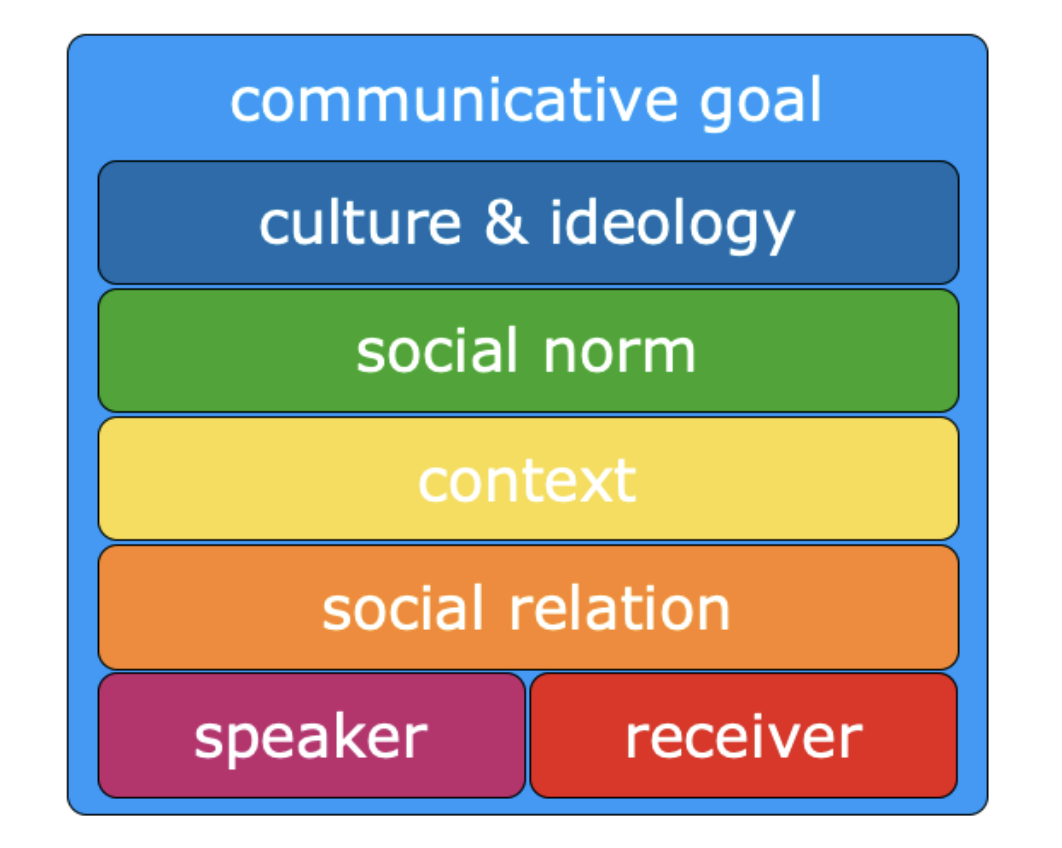
\includegraphics[width=0.3\textwidth,height=\textheight]{src/Figures/seven-taxonomy.png}

}

\caption{\label{fig-taxonomy}Taxonomy of social factors}

\end{figure}%

This taxonomy illustrates both the current limitations and progressions
in NLP as they pertain to each of these factors. The primary aim is to
motivate the NLP community to integrate these social factors more
effectively, thereby advancing towards a level of language understanding
that more closely resembles human capabilities. The characteristics of
speakers, encompassing variables such as age, gender, ethnicity, social
class, and dialect, play a crucial role in language processing. Certain
languages or dialects, often categorized as low-resource, are spoken by
vulnerable populations that require special consideration in NLP
systems. In many cases, the dominant culture and values are
over-represented, leading to an inadvertent marginalization of minority
perspectives. These minority voices must be not only recognized but also
given equitable representation in language models. Additionally, norms
and context are vital components in understanding linguistic behavior.
They dictate the appropriateness of language use in various social
situations and settings. Recognizing and adapting to these norms is a
critical aspect of developing socially aware NLP systems that can
effectively function across diverse social environments.

\subsubsection{Human-Centered}\label{human-centered}

The Human-Centered aspect of NLP development emphasizes the creation of
language models that prioritize the needs, preferences, and well-being
of human users. This involves integrating human-centered design
principles throughout the development stages of LLMs, which are
described as follows:

\begin{itemize}
\item
  \textbf{Task Formulation stage:} Human-centered NLP development begins
  with understanding the specific problems and contexts in which users
  operate. This involves collaborating with end-users to identify their
  needs and challenges, ensuring that the tasks addressed by the models
  are relevant and meaningful to them. By engaging with users early in
  the process, developers can create models that are not only
  technically robust but also practically useful.
\item
  \textbf{Data Collection stage:} Human-centered principles ensure that
  the data used to train models is representative of the diverse user
  population. This includes collecting data from various demographic
  groups, languages, and cultural contexts to avoid biases that could
  lead to unfair or harmful outcomes. Ethical considerations are
  paramount, ensuring that data is collected with informed consent and
  respecting users' privacy.
\item
  \textbf{Data Processing} in a human-centered approach involves
  carefully curating and annotating data to reflect the nuances of human
  language and behavior. This step includes filtering out potentially
  harmful content, addressing imbalances in the data, and ensuring that
  the labels and annotations are accurate and meaningful. By involving
  human annotators from diverse backgrounds, developers can capture a
  wider range of perspectives and reduce the risk of biased outputs.
\item
  \textbf{Model Training} with a human-centered focus involves
  incorporating feedback from users and domain experts to fine-tune the
  models. This iterative process ensures that the models remain aligned
  with users' needs and preferences. Techniques such as active learning,
  where the model queries users for the most informative examples, can
  be employed to improve the model's performance.
\item
  \textbf{Model Evaluation} in a human-centered framework goes beyond
  traditional metrics like accuracy and F1-score. It includes assessing
  the model's impact on users, its fairness, and its ability to handle
  real-world scenarios. User studies and A/B testing can provide
  valuable insights into how the model performs in practice and how it
  affects users' experiences.
\item
  \textbf{Deployment} of human-centered NLP models involves continuous
  monitoring and feedback loops to ensure that the models remain
  effective and aligned with users' needs over time. This includes
  setting up mechanisms for users to report issues and provide feedback,
  which can then be used to update and improve the models. Ensuring
  transparency in how the models operate and how user data is used also
  fosters trust and acceptance among users.
\end{itemize}

\subsubsection{Positively Impactful}\label{positively-impactful}

Building on the human-centered approach, it is crucial to consider how
language models can be utilized and the broader impacts they can have on
society.

\textbf{Utilization:} LLMs offer socially beneficial applications across
various domains such as public policy, mental health, and education. In
public policy, they assist in analyzing large volumes of data to inform
decision-making processes. In mental health, LLMs can provide
personalized therapy and even train therapists by simulating patient
interactions. In the education sector, they enable personalized learning
experiences and language assistance, making education more accessible
and effective. These examples demonstrate the versatility of LLMs in
contributing positively to critical areas of human life.

\textbf{Impact:} The deployment of NLP models, especially LLMs, has
significant societal impacts. Positively, they enhance human
productivity and creativity, offering tools and insights that streamline
processes and foster innovative thinking. LLMs serve as powerful aids in
various sectors, from education to industry, enhancing efficiency and
enabling new forms of expression and problem-solving. it is essential to
acknowledge the potential negative impacts. One major concern is the
ability of LLMs to generate and spread misinformation. As these models
become more adept at producing human-like text, distinguishing between
AI-generated and human-created content becomes increasingly challenging.
This raises issues of trust and reliability, with the risk of widespread
dissemination of false or misleading information, which could have
significant adverse effects on individuals and society.

By considering both the utilization and impact of LLMs, we can better
harness their potential for positive societal contributions while
mitigating the risks associated with their deployment. In conclusion, by
thoughtfully integrating human-centered principles and ensuring positive
impacts through feedback collection and ethical considerations, we can
develop language models that not only enhance human well-being but also
align closely with societal values. Building on these foundational
principles, we now turn our attention to Adaptive User Interfaces, which
exemplify the practical application of these concepts by personalizing
interactions and improving user experiences in dynamic environments.

\subsection{Adaptive User Interfaces}\label{adaptive-user-interfaces}

Adaptive user interfaces (AUIs) represent a significant advancement in
personalizing user experiences by learning and adapting to individual
preferences. This section will discuss the methodologies and
applications of AUIs, highlighting their role in enhancing human-AI
interaction through intelligent adaptation. The integration of AUIs
within human-centered design paradigms ensures that AI systems not only
meet user needs but also anticipate and adapt to their evolving
preferences, thus maximizing positive human impact. Nowadays, consumers
have more choices than ever and the need for personalized and
intelligent assistance to make sense of the vast amount of information
presented to them is clear.

\subsubsection{Key ideas}\label{key-ideas}

In general, personalized recommendation systems require a model or
profile of the user. We categorize modeling approaches into four groups.

\begin{enumerate}
\def\labelenumi{\arabic{enumi}.}
\item
  User-created profiles (usually done manually).
\item
  Manually defined groups (stereotypes) that each user is classified
  into.
\item
  Automatically learned groups (stereotypes) that each user is
  classified into.
\item
  Adaptively learned individual user models from interactions with the
  recommendation system.
\end{enumerate}

The last approach is referred to as \emph{adaptive user interfaces}.
This approach promises that each user is given the most personalization
possible, leading to better outcomes. In this session, we discuss
recommendation systems that adaptively learn an individual's preferences
and use that knowledge to intelligently recommend choices that the
individual is more inclined to like.

The problem of learning individual models can be formalized, given as
follows:

\begin{itemize}
\item
  a set of tasks requiring a user decision,
\item
  a description for each task,
\item
  a history of the user's decision on each task,
\end{itemize}

So then we can find a function that maps from task description
(features) to user decisions. The task can be described from
crowd-sourced data (a collaborative approach) or the measurable features
of the task (a content-based approach). The content-based approaches for
describing tasks will be focused on in this session. After understanding
the framework for adaptive user interfaces now it is a good point to
give some example applications to help ground the future discussion.
Adaptive user interfaces have been developed for

\begin{itemize}
\item
  Command and form completion
\item
  Email filtering and filing
\item
  News selection and layout
\item
  Browsing the internet
\item
  Selecting movies and TV shows
\item
  Online shopping
\item
  In-car navigation
\item
  Interactive scheduling
\item
  Dialogue systems
\end{itemize}

among many other applications.

\subsubsection{Design}\label{design}

The goal of an adaptive user interface is to create a software tool that
reduces human effort by acquiring a user model based on past user
interactions. This is analogous to the goal of machine learning (ML)
which is to create a software tool that improves some task performance
by acquiring knowledge based on partial task experience. The design of
an adaptive user interface can be broken up into six steps:

\begin{enumerate}
\def\labelenumi{\arabic{enumi}.}
\item
  \textbf{Formulating the Problem:} Given some task that an intelligent
  system could aid, the goal is to find a formulation that lets the
  assistant improve its performance over time by learning from
  interactions with a user. In this step the designer has to make design
  choices about what aspect of user behavior is predicted, and what is
  the proper level of granularity for description (i.e.~what is a
  training example). This step usually involves formulating the problem
  into some sort of supervised learning framework.
\item
  \textbf{Engineering the Representation:} At this stage we have a
  formulation of a task in ML terms and we need to represent the
  behavior and user model in such a way that makes computational
  learning not only tractable but as easy as possible. In this step, the
  designer has to make design choices about what information is used to
  make predictions, and how that information is encoded and passed to
  the model.
\item
  \textbf{Collecting User Traces:} In this third step the goal is to
  find an effective way to collect traces (samples) of user behavior.
  The designer must choose how to translate traces into training data
  and also how to elicit traces from a user. An ideal adaptive user
  interface places no extra effort on the user to collect such traces.
\item
  \textbf{Modeling the User:} In this step the designer must decide what
  model class to use (neural network, decision tree, graphical model,
  etc.) and how to train the model (optimizer, step size, batch size,
  etc.). This step in the design process is usually given too much
  importance in academia. It is quite often the case that the success of
  an adaptive user interface is more sensitive to the other design
  steps.
\item
  \textbf{Using the Model Effectively:} At this stage the designer must
  decide how the model will be integrated into a software tool.
  Specifically, when and how is the model evaluated and how is the
  output of the model presented to the user? In addition, the designer
  must consider how to handle situations in which the model predictions
  are wrong. An ideal adaptive user interface will let the user take
  advantage of good predictions and ignore bad ones.
\item
  \textbf{Gaining User Acceptance:} The final step in the design process
  is to get users to try the system and ultimately adopt it. The initial
  attraction of users is often a marketing problem, but to retain users
  the system must be well-designed and easy to use.
\end{enumerate}

\subsubsection{Applications}\label{applications-1}

After understanding the design of Adaptive User Interfaces, let's take a
look at how we can apply it to real-world problems. We will summarize
and analyze three different application areas of learning human
preferences, which are driving route advisor
(\citeproc{ref-rogers1999adaptive}{Rogers, Fiechter, and Langley 1999}),
destination selection (\citeproc{ref-langley1999adaptive}{Langley et al.
1999}), and resource scheduling
(\citeproc{ref-gervasio1999learning}{Gervasio, Iba, and Langley 1999}).

\textbf{1. Driving Route Advisor:} The task of route selection involves
determining a desirable path for a driver to take from their current
location to a chosen destination, given the knowledge of available roads
from a digital map. While computational route advisors exist in rental
cars and online, they cannot personalize individual drivers'
preferences, which is a gap that adaptive user interfaces aim to fill by
learning and recommending routes tailored to the driver's unique choices
and behaviors.

Here is an approach to route selection through learning individual
drivers' route preferences.

\begin{itemize}
\item
  Formulation: Learn a ``subjective'' function to evaluate entire
  routes.
\item
  Representation: Global route features are computable from digital
  maps.
\item
  Data collection: Preference of one complete route over another.
\item
  Induction: A method for learning weights from preference data.
\item
  Using model: Apply subjective function to find ``optimal'' route.
\end{itemize}

This method aims to learn a user model that considers the entirety of a
route, thereby avoiding issues like data fragmentation and credit
assignment problems.

The design choices are incorporated into
(\citeproc{ref-rogers1999adaptive}{Rogers, Fiechter, and Langley 1999}),
which: models driver preferences in terms of 14 global route features;
gives the driver two alternative routes he might take; lets the driver
refine these choices along route dimensions; uses driver choices to
refine its model of his preferences; and invokes the driver model to
recommend future routes. We note that providing drivers with choices
lets the system collect data on route preferences in an unobtrusive
manner. The interface of the application is presented in
Figure~\ref{fig-exp-1}.

\begin{figure}

\centering{

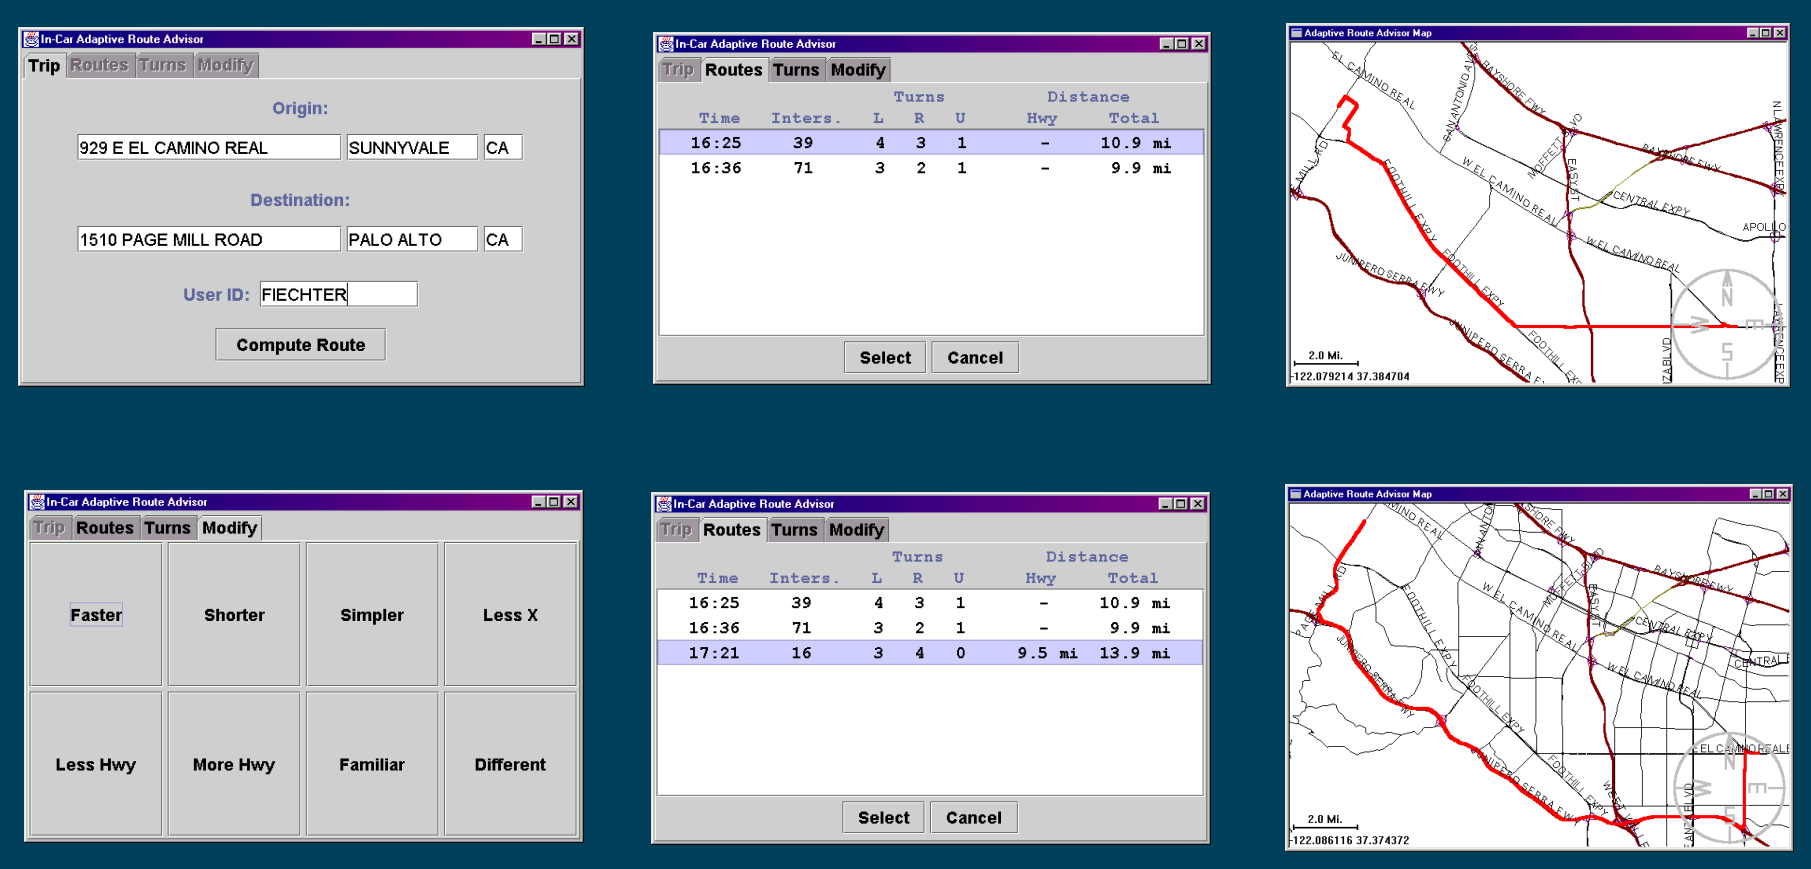
\includegraphics[width=0.8\textwidth,height=\textheight]{src/Figures/example-1.png}

}

\caption{\label{fig-exp-1}The adaptive route advisor.}

\end{figure}%

In driving route advisor task (\citeproc{ref-rogers1999adaptive}{Rogers,
Fiechter, and Langley 1999}), a linear model is used for predicting the
cost of a route based on the time, distance, number of intersections,
and the number of turns. The system uses each training pair as a
constraint on the weights found during the learning process. The
experimental results are shown in the \textbf{?@fig-exp-2}.

(Left) Experiments with 24 subjects show the Route Advisor improves its
predictive ability rapidly with experience. (Right) Analyses also show
that personalized user models produce better results than generalized
models, even when given more data.

\textbf{2. Destination Selection:} The task of destination selection
involves assisting a driver in identifying one or more suitable
destinations that fulfill a specific goal, such as finding a place to
eat lunch, based on the driver's current location and knowledge of
nearby options. While there are many recommendation systems online,
including those for restaurants, they are not ideally suited for drivers
due to the driving environment's demand for limited visual attention,
thus necessitating a more tailored and accessible approach for in-car
use.

One approach to destination recommendation can be cast as:

\begin{itemize}
\item
  Formulation: Learn to predict features the user cares about in items.
\item
  Representation: Conditions/weights on attributes and values.
\item
  Data collection: Converse with the user to help him make decisions,
  noting whether he accepts or rejects questions and items.
\item
  Induction: Any supervised induction method.
\item
  Using model: Guide the dialogue by selecting informative questions and
  suggesting likely values.
\end{itemize}

This design relies on the idea of a conversational user interface.
Spoken-language versions of this approach appear well suited to the
driving environment.

This approach is implemented in
(\citeproc{ref-langley1999adaptive}{Langley et al. 1999}), where it
engages in spoken conversations to help a user refine goals;
incorporates a dialogue model to constrain this process; collects and
stores traces of interaction with the user; and personalizes both its
questions and recommended items. Their work focused on recommending
restaurants to users who want advice about where to eat. This approach
to recommendation would work well for drivers, it also has broader
applications. We present experimental results in

(Left) Speech Acts Per Conversation. (Right) Time Per Conversation.

\textbf{3. Resource Scheduling:} The task of resource scheduling
describes the challenge of allocating a limited set of resources to
complete a set of tasks or jobs within a certain time frame, while also
considering the constraints on both the jobs and the resources. Although
automated scheduling systems are prevalent in various industries and
some interactive schedulers exist, there is a distinct need for systems
that can create personalized schedules reflecting the unique preferences
of individual users.

An approach to personalized scheduling can be described as:

\begin{itemize}
\item
  Formulation: Learn a utility function to evaluate entire schedules.
\item
  Representation: Global features are computable from the schedule.
\item
  Data collection: Preference of one candidate schedule over others.
\item
  Induction: A method for learning weights from preference data.
\item
  Using model: Apply the `subjective' function to find a good schedule.
\end{itemize}

We note that this method is similar to that in the Adaptive Route
Advisor. However, it assumes a search through a space of complete
schedules (a repair space), which requires some initial schedule. This
approach is implemented in
(\citeproc{ref-gervasio1999learning}{Gervasio, Iba, and Langley 1999}),
where the interactive scheduler retrieves an initial schedule from a
personalized case library; suggests to the user improved schedules from
which to select; lets the user direct search to improve on certain
dimensions; collects user choices to refine its personalized utility
function; stores solutions in the case base to initialize future
schedules; and invokes the user model to recommend future schedule
repairs. As before, providing users with choices lets the system collect
data on schedule preferences unobtrusively. An example of the interface,
and the experimental results are shown in \textbf{?@fig-exp-3}.

(Left) The interface of the INCA: Interactive Scheduling {}. (Right)
Experiments with INCA suggest that retrieving personalized schedules
helps users more as task difficulty increases. These experimental
studies used a mixture of human and synthetic subjects.

\subsubsection{Limitations}\label{limitations}

The challenges of adaptive interfaces may involve: conceptualizing user
modeling as a task suitable for inductive learning, crafting
representations that facilitate the learning process, gathering training
data from users in a way that doesn't intrude on their experience,
applying the learned user model effectively, ensuring the system can
learn in real-time, and dealing with the necessity of learning from a
limited number of training instances. These challenges are not only
pertinent to adaptive interfaces but also intersect with broader
applications of machine learning, while also introducing some unique
issues. However, new sensor technology can bring promises to adaptive
interfaces. Adaptive interfaces rely on user traces to drive their
modeling process, so they stand to benefit from developments like GPS
and cell phone locators, robust software for speech recognition,
accurate eye and head trackers, real-time video interpreters, wearable
body sensors (GSR, heart rate), and portable brain-wave sensors. As
those devices become more widespread, they will offer new sources of
data and support new types of adaptive services. In addition, adaptive
interfaces can be viewed as a form of cognitive simulation that
automatically generates knowledge structures to learn user preferences.
They are capable of making explicit predictions about future user
behavior and explaining individual differences through the process of
personalization. This perspective views adaptive interfaces as tools
that not only serve functional purposes but also model the psychological
aspects of user interaction. Two distinct approaches within cognitive
simulation are related to adaptive interfaces: \emph{process} models
that incorporate fundamental architectural principles, and
\emph{content} models that operate at the knowledge level, focusing on
behavior. We note that both of them have roles to play, but content
models are more relevant to personalization and adaptive interfaces.

In conclusion, adaptive user interfaces represent a significant
advancement in creating personalized and efficient interactions between
humans and technology. By leveraging modern sensor technologies and
cognitive simulation approaches, these interfaces can dynamically learn
and adapt to individual user preferences, enhancing overall user
experience and system effectiveness. The methodologies discussed, from
conceptualizing user models to collecting and utilizing user feedback,
form the foundation of this innovative approach. As we transition to the
next section, we will explore practical applications and real-world
implementations of these human-centered AI principles through detailed
case studies, illustrating the tangible impact of adaptive interfaces in
various domains.

\subsection{Case Studies in Human-Centered
AI}\label{case-studies-in-human-centered-ai}

In this section, we examine practical examples that illustrate the
application of human-centered principles in the development and
deployment of AI systems. By examining these case studies, we aim to
provide concrete insights into how AI technologies can be designed and
implemented to better align with human values, enhance inclusivity, and
address the specific needs of diverse user groups. The following case
studies highlight different approaches and methodologies used to ensure
that AI systems are not only effective but also considerate of the human
experience.

\subsubsection{LaMPost Case Study}\label{lampost-case-study}

In our exploration of human-centered AI design, it is crucial to examine
how metrics can be improved to better capture the human experience and
address the shortcomings of traditional evaluation methods. The LaMPost
case study (\citeproc{ref-goodman_lampost_2022}{Goodman et al. 2022})
exemplifies this effort by focusing on the development of an AI
assistant designed to aid individuals with dyslexia in writing emails.
This case is particularly relevant to our discussion because it
highlights the importance of human-centered principles in AI
development, especially in creating tools that cater to specific
cognitive differences and enhance user experience.

Dyslexia is a cognitive difference that affects approximately 15 percent
of language users, with varying degrees of impact on speaking, spelling,
and writing abilities. It is a spectrum disorder, meaning symptoms and
severity differ among individuals. More importantly, dyslexia is not an
intellectual disability; many individuals with dyslexia possess high
intelligence. Given the significant number of people affected by
dyslexia, it is essential to develop AI tools that support their unique
needs and enhance their daily tasks.

The LaMPost project sought to answer the question, ``How can LLMs be
applied to enhance the writing workflows of adults with dyslexia?'' To
address this, researchers employed a participatory design approach,
involving employees with dyslexia from their company (Google) in the
study. This approach ensured that the development process was inclusive
and responsive to the actual needs and preferences of the dyslexic
community. By focusing on the real-world application of LLMs in aiding
email writing for dyslexic individuals, LaMPost serves as a powerful
example of how AI can be designed to better capture and enhance the
human experience.

The figure below allows users to see suggestions for rewriting selected
text, helping them identify main ideas, suggest possible changes, and
rewrite their selections to improve clarity and expression.

\begin{figure}[H]

{\centering \includegraphics{src/Figures/lampost_fig3.png}

}

\caption{The Suggest Possible Changes feature from LaMPost.}

\end{figure}%

The table below categorizes the challenges faced by users at different
writing levels and the strategies they can use to overcome these
challenges, illustrating the varied support needs addressed by LaMPost

Writing level

Examples of Challenges

Strategies

high

expressing ideas

``word faucet'', ASR dictation

ordering ideas

post-it outlining

low

appropriate language

proofreading

paraphrasing

feedback

User challenged and strategies in LaMPost.

Next, they ran a focus group to get initial ideas from members of the
dyslexic community. This focus group helped them figure out what to
measure and added the second research question: ``How do adults with
dyslexia feel about LLM-assisted writing?'' In other words, how does the
LLM impact users' feelings of satisfaction, self-expression,
self-efficacy, autonomy, and control?

From this focus group, they went and created a prototype to answer the
desires of the group. They included three features in their prototype
model. One feature was: \emph{identifying main ideas}. They focused on
this to support overall clarity and organization of high-level ideas of
the user. Another feature was \emph{suggest possible changes}. They
focused on this because users wanted to identify high-level adjustments
to improve their writing. The last feature they added was \emph{rewrite
my selections}. They added this because users wanted help expressing
ideas with a desired phrasing tone or style. This feature generated a
rewrite based on a command you gave it.

With the prototype, the researchers evaluated again with 19 participants
with dyslexia from outside their organization. They did a three-part
study, including a demonstration and background on the system (25 min).
Then they did a writing exercise with two real tasks (emails) each user
had to do in the real world (25 min). For example, one task might have
been to write an email to the principal of their child's school to ask
for a meeting. Then, the researchers did another follow-up interview for
more qualitative data, e.g.~to ask about specific choices users made
when interacting with the model (25 min).

LaMPost's design prioritized autonomy by allowing users to choose the
best option for their writing. One successful thing is that most users
felt in control while writing. Users found that numerous options were
helpful to filter through poor results. However, participants said the
selection process was cognitively demanding and time-consuming. As we
all know, features identified in LaMPost are all over the place, such as
in Google Docs. Nonetheless, there remain many questions about the
balance between automated writing and providing more control to the end
users.

How could researchers hone in on this trade-off between \textbf{the ease
of automated writing} and \textbf{providing control to end-users}?\\
You will need to design a study to approach this question.

\begin{itemize}
\item
  Identify your research question, hypotheses, and the methods that you
  will use. (Hint: use the HCI methods described in the previous
  section.)
\item
  Scope the domain of your study appropriately---more broadly than
  dyslexia but not so broadly to be meaningless.
\item
  What domains will you include? (E.g. students use ChatGPT for
  assignments, doctors use an LLM to write notes, etc.)
\end{itemize}

In this way, both the case study of LaMPost and its presaging of greater
trends in LLM interfaces recapitulate the maxim of HCI: HCI is a cycle.
You design a potential system, prototype it, get feedback from people,
and iterate constantly. Next, we will explore two case studies that
exemplify the application of human-centered principles in NLP. These
case studies illustrate how LLMs can be adapted to foster social
inclusivity and provide training in social skills.

\subsubsection{Multi-Value and DaDa: Cross-Dialectal English
NLP}\label{multi-value-and-dada-cross-dialectal-english-nlp}

English NLP systems are largely trained to perform well in Standard
American English - the form of written English found in professional
settings and elsewhere. Not only is Standard American English the most
well-represented form of English in textual datasets but NLP engineers
and researchers often filter dialectal and vernacular English examples
from their datasets to improve performance on SAE benchmarks. As a
result, NLP systems are generally less performant when processing
dialectal inputs than SAE inputs. This performance gap is observable
over various benchmarks and tasks, like the SPIDER benchmark.
(\citeproc{ref-spider}{Chang et al. 2023})

\begin{figure}[H]

{\centering \includegraphics[width=1\textwidth,height=\textheight]{src/Figures/MV2.png}

}

\caption{Stress test reveals worse performance on the SPIDER benchmark
with synthetic dialectical examples than with SAE.}

\end{figure}%

As natural language systems become more pervasive, this performance gap
increasingly represents a real allocational harm against dialectal
English speakers --- these speakers are excluded from using helpful
systems and assistants. Multi-Value is a framework for evaluating
foundation language models on dialectic input, and DADA is a framework
for adapting LLMs to improve performance on dialectic input.

\textbf{Synthetic Dialectal Data}

Ziems et al.~(2023) create synthetic dialectal data for several English
dialects (Appalachian English, Chicano English, Indian English,
Colloquial Singapore English, and Urban African American
English).(\citeproc{ref-mv}{Ziems et al. 2023}) They created synthetic
data based on transforming SAE examples to have direct evaluation
comparisons. These synthetic examples were created by leveraging known
linguistic features of the dialects, such as negative concord in UAAVE.
Figure~\ref{fig-features_dialects} maps out the presence of various
linguistic features.

\begin{figure}

\centering{

\includegraphics[width=1\textwidth,height=\textheight]{src/Figures/MV1.png}

}

\caption{\label{fig-features_dialects}A comparative distribution of
features in five dialects.}

\end{figure}%

This synthetic data, while somewhat limited in the variety of samples.
can produce and create realistic examples for benchmarking LM
performance. Figure~\ref{fig-synthetic_example} demonstrates creating a
synthetic dialectic example using the `give passive' linguistic feature,
illustrating the transformation process from SAE to a vernacular form.

\begin{figure}

\centering{

\includegraphics[width=0.4\textwidth,height=\textheight]{src/Figures/MV3.png}

}

\caption{\label{fig-synthetic_example}Execution of a sample transform
using a documented linguistic feature.}

\end{figure}%

\textbf{Feature Level Adapters} One approach to the LLM adaption task
would be to train an adapter for each dialect using a
parameter-efficient fine-tuning method like low-rank adapters.
(\citeproc{ref-lora}{Hu et al. 2021}) While adapters can certainly
bridge the gap between SAE LMs and dialect inputs, this approach suffers
from a couple of weaknesses, namely:

\begin{itemize}
\item
  Individually trained adapters do not leverage similarities between
  low-resource dialects. Transfer learning is often helpful for training
  low-resource languages and dialects.
\item
  The model needs to know which adapter to use at inference time. This
  presupposes that we can accurately classify the dialect --- sometimes
  based on as little as one utterance. This classification is not always
  possible --- a more general approach is needed.
\end{itemize}

Therefore, Liu et al.~(2023) propose a novel solution --- DADA: Dialect
Adaption via Dynamic Aggregation of Linguistic Rules.
(\citeproc{ref-dada}{Liu, Held, and Yang 2023}) DADA trains adapters on
the linguistic feature level rather than the dialect level. The model
can use multiple linguistic feature adapters via an additional fusion
layer. They can therefore train using multi-dialectical data and cover
linguistic variation via a comprehensive set of roughly 200 adapters.
DADA saw an improvement in performance over single-dialect adapters for
most dialects, as shown in Figure~\ref{fig-dada_performance}.

\begin{figure}

\centering{

\includegraphics[width=0.4\textwidth,height=\textheight]{src/Figures/MV4.png}

}

\caption{\label{fig-dada_performance}Execution of a sample transform
using a documented linguistic feature.}

\end{figure}%

The Multi-Value and DADA case study underscores the importance of
designing NLP systems that are inclusive and representative of diverse
language users. By addressing the performance gaps in handling dialectal
inputs, this case study highlights the necessity of incorporating
diverse linguistic data and creating adaptable systems. This approach
enhances AI functionality and accessibility, ensuring it respects and
reflects linguistic diversity. Ultimately, the study reinforces
human-centered design principles, demonstrating how AI can be tailored
to better serve and empower all users. Moving forward, we will explore
how LLMs can be utilized for social skill training, showcasing their
potential to improve human interactions.

\subsubsection{Social Skill Training via
LLMs}\label{social-skill-training-via-llms}

The emergence of Large Language Models (LLMs) marks a significant
milestone in the field of social skills training. This case study
explores the potential of LLMs to augment social skill development
across diverse scenarios. More specifically, we discuss a dual-framework
approach, where two distinct LLMs operate in tandem as a Partner and a
Mentor, guiding human learners in their journey towards improved social
interaction. In this framework, we have two agents which are

\begin{itemize}
\item
  \textbf{AI Partner}: LLM-empowered agents that users can engage with
  across various topics. This interactive model facilitates practical,
  conversation-based learning, enabling users to experiment with
  different communication styles and techniques or practice and develop
  specific skills in real-world scenarios in a safe, AI-mediated
  environment.
\item
  \textbf{AI Mentor}: An LLM-empowered entity designed to provide
  constructive, personalized feedback based on the interaction of users
  and the AI Partner. This mentor analyzes conversation dynamics,
  identifies areas for improvement, offers tailored advice, and guides
  users toward effective social strategies and improved interaction
  skills.
\end{itemize}

For example, in conflict resolution, individuals learning to handle
difficult conversations can use the AI Partner to simulate interactions
with a digitalized partner. As a Conflict Resolution Expert, the AI
Mentor helps analyze these interactions, offering strategies to navigate
conflicts effectively.

In the educational sector, K-12 teachers aiming to incorporate more
growth-mindset language into their teaching can practice with a
digitalized student. An experienced teacher or mentor, represented by
the AI Mentor, provides insights on effective communication and teaching
methods. For negotiation training, students preparing to negotiate their
first job offers can engage in simulated negotiations with a digitalized
HR representative through the AI Partner. As a Negotiation Expert, the
AI Mentor then offers guidance on negotiation tactics, helping students
effectively articulate their values and negotiate job terms. Lastly, in
therapy training, novice therapists can interact with a digitalized
patient via the AI Partner to practice therapy sessions. The AI Mentor,
functioning as a Therapy Coach, then reviews these sessions, providing
feedback and suggestions on enhancing therapeutic techniques and patient
engagement.

\textbf{CARE: Therapy Skill Training} Hsu et al.~(2023) introduced CARE
(\citeproc{ref-hsu2023helping}{Hsu et al. 2023}), a framework designed
for therapy skill training. This framework leverages a simulated
environment, enabling counselors to practice their skills without the
risk of harming real individuals. An integral component of CARE is the
AI Mentor, which offers invaluable feedback and guidance during the
training process. See Figure~\ref{fig-care} for the overview of the
framework.

\begin{figure}

\centering{

\includegraphics[width=0.45\textwidth,height=\textheight]{src/Figures/care.png}

}

\caption{\label{fig-care}CARE Framework}

\end{figure}%

CARE's primary function is for novice therapists and counselors to
assess and determine the most effective counseling strategies tailored
to specific contexts. It provides counselors with customized example
responses, which they can adopt, adapt, or disregard when interacting
with a simulated support seeker. This approach is deeply rooted in the
principles of Motivational Interviewing and utilizes a rich dataset of
counseling conversations combined with LLMs. The effectiveness of CARE
has been established through rigorous quantitative evaluations and
qualitative user studies, which included simulated chats and
semi-structured interviews. Notably, CARE has shown significant benefits
in aiding novice counselors. From the assessment, counselors chose to
use CARE 93\% of the time, directly used a CARE response without editing
60\% of the time, and sent more extended responses with CARE.
Qualitatively, counselors noted several advantages of CARE, such as its
ability to refresh memory on various strategies, inspire innovative
responses, boost confidence, and save time during consultations.
However, there were some drawbacks, including potential disruptions in
the thought process, perceived limitations in response options, the
requirement for decision-making, and the time needed to review
suggestions. Overall, the framework is particularly beneficial for
therapists new to the field, offering them a supportive and educational
tool to enhance their counseling skills effectively.

\section{Practice Exercises}\label{practice-exercises}

\section*{References}\label{bibliography-5}
\addcontentsline{toc}{section}{References}

\markright{References}

\phantomsection\label{refs-5}
\begin{CSLReferences}{1}{0}
\bibitem[\citeproctext]{ref-amodei2016concrete}
Amodei, Dario, Chris Olah, Jacob Steinhardt, Paul Christiano, John
Schulman, and Dan Mane. 2016. {``Concrete Problems in AI Safety.''}
\emph{arXiv Preprint arXiv:1606.06565}.

\bibitem[\citeproctext]{ref-angwin_machine_2016}
Angwin, Julia, Jeff Larson, Surya Mattu, and Lauren Kirchner. 2016.
{``Machine Bias.''} \emph{ProPublica}.

\bibitem[\citeproctext]{ref-arcas_can_2022}
Arcas, Blaise Aguera y. 2022. {``Can Machines Learn How to Behave?''}
\emph{Medium}.
\url{https://medium.com/@blaisea/can-machines-learn-how-to-behave-42a02a57fadb}.

\bibitem[\citeproctext]{ref-aristotle_nicomachean_350}
Aristotle. 350 B.C.E. \emph{Nicomachean Ethics}. translated by W.D.
Ross.

\bibitem[\citeproctext]{ref-bai_constitutional_2022}
Bai, Yuntao, Saurav Kadavath, Sandipan Kundu, Amanda Askell, Jackson
Kernion, Andy Jones, Anna Chen, Anna Goldie, Azalia Mirhoseini, and
Cameron McKinnon. 2022. {``Constitutional Ai: {Harmlessness} from Ai
Feedback.''} \emph{arXiv Preprint arXiv:2212.08073}.

\bibitem[\citeproctext]{ref-barocas_fairness_2019}
Barocas, Solon, Moritz Hardt, and Arvind Narayanan. 2019. \emph{Fairness
and Machine Learning}. fairmlbook.org.

\bibitem[\citeproctext]{ref-bernstein2010soylent}
Bernstein, Michael S., Greg Little, Robert C. Miller, Bjorn Hartmann,
Mark S. Ackerman, David R. Karger, David Crowell, and Katrina Panovich.
2010. {``Soylent: A Word Processor with a Crowd Inside.''} In
\emph{Proceedings of the 23nd Annual ACM Symposium on User Interface
Software and Technology}. ACM.

\bibitem[\citeproctext]{ref-binns_fairness_2018}
Binns, Reuben. 2018. {``Fairness in Machine Learning: Lessons from
Political Philosophy.''} In \emph{Proceedings of the 2018 Conference on
Fairness, Accountability, and Transparency}, 149--59.

\bibitem[\citeproctext]{ref-bostrom2014superintelligence}
Bostrom, Nick. 2014. \emph{Superintelligence: Paths, Dangers,
Strategies}. Oxford University Press.

\bibitem[\citeproctext]{ref-brown2019machine}
Brown, Daniel S, and Scott Niekum. 2019. {``Machine Teaching for Inverse
Reinforcement Learning: Algorithms and Applications.''} In
\emph{Proceedings of the AAAI Conference on Artificial Intelligence},
33:7749--58.

\bibitem[\citeproctext]{ref-brown2021value}
Brown, Daniel S, Jordan Schneider, Anca Dragan, and Scott Niekum. 2021.
{``Value Alignment Verification.''} In \emph{International Conference on
Machine Learning}, 1105--15. PMLR.

\bibitem[\citeproctext]{ref-tuskegee}
Centers for Disease Control and Prevention. 2023. {``The u.s. Public
Health Service Untreated Syphilis Study at Tuskegee.''}
\url{https://www.cdc.gov/tuskegee/index.html}.

\bibitem[\citeproctext]{ref-spider}
Chang, Shuaichen, Jun Wang, Mingwen Dong, Lin Pan, Henghui Zhu,
Alexander Hanbo Li, Wuwei Lan, et al. 2023. {``Dr.spider: A Diagnostic
Evaluation Benchmark Towards Text-to-SQL Robustness.''}
\url{https://arxiv.org/abs/2301.08881}.

\bibitem[\citeproctext]{ref-chowdhery_palm_2022}
Chowdhery, Aakanksha, Sharan Narang, Jacob Devlin, Maarten Bosma, Gaurav
Mishra, Adam Roberts, Paul Barham, et al. 2022. {``{PaLM}: {Scaling}
{Language} {Modeling} with {Pathways}.''} \emph{arXiv:2204.02311
{[}Cs{]}}, April. \url{http://arxiv.org/abs/2204.02311}.

\bibitem[\citeproctext]{ref-christianoclarifying}
Christiano, Paul. 2018. {``Clarifying {`AI Alignment'}.''}
\url{https://ai-alignment.com/clarifying-ai-alignment-cec47cd69dd6}.

\bibitem[\citeproctext]{ref-christiano2017deep}
Christiano, Paul F, Jan Leike, Tom Brown, Miljan Martic, Shane Legg, and
Dario Amodei. 2017. {``Deep Reinforcement Learning from Human
Preferences.''} \emph{Advances in Neural Information Processing Systems}
30.

\bibitem[\citeproctext]{ref-clark2016faulty}
Clark, Jack, and Dario Amodei. 2016. {``Faulty Reward Functions in the
Wild.''} \emph{OpenAI Blog}.

\bibitem[\citeproctext]{ref-dworkin1988theory}
Dworkin, Gerald. 1988. \emph{The Theory and Practice of Autonomy}.
Cambridge University Press.

\bibitem[\citeproctext]{ref-everitt2018alignment}
Everitt, Tom, and Marcus Hutter. 2018. {``The Alignment Problem for
Artificial Intelligence.''} In \emph{Advances in Neural Information
Processing Systems}, 1--8.

\bibitem[\citeproctext]{ref-floridi2011ethics}
Floridi, Luciano. 2011. \emph{The Ethics of Information}. Oxford
University Press.

\bibitem[\citeproctext]{ref-frankena1973ethics}
Frankena, William K. 1973. \emph{Ethics}. Prentice Hall.

\bibitem[\citeproctext]{ref-friedman_value_2008}
Friedman, Batya, Peter H. Kahn, and Alan Borning. 2008. {``Value
Sensitive Design and Information Systems.''} In \emph{The Handbook of
Information and Computer Ethics}. John Wiley \& Sons.

\bibitem[\citeproctext]{ref-gervasio1999learning}
Gervasio, Melinda T, Wayne Iba, and Pat Langley. 1999. {``Learning User
Evaluation Functions for Adaptive Scheduling Assistance.''} In
\emph{ICML}, 152--61. Citeseer.

\bibitem[\citeproctext]{ref-goodall_machine_2014}
Goodall, Noah J. 2014. {``Machine Ethics and Automated Vehicles.''} In
\emph{Road Vehicle Automation}, 93--102. Springer.

\bibitem[\citeproctext]{ref-goodman_lampost_2022}
Goodman, Steven, Erin Buehler, Patrick Clary, Andy Coenen, Aaron Michael
Donsbach, Tiffanie Horne, Michal Lahav, et al. 2022. {``LaMPost:
Evaluation of an AI-Assisted Writing Email Editor Prototype for Adults
with Dyslexia.''}

\bibitem[\citeproctext]{ref-hadfield2016cooperative}
Hadfield-Menell, Dylan, Stuart J Russell, Pieter Abbeel, and Anca
Dragan. 2016. {``Cooperative Inverse Reinforcement Learning.''}
\emph{Advances in Neural Information Processing Systems} 29.

\bibitem[\citeproctext]{ref-hardt_patterns_2021}
Hardt, Moritz, and Benjamin Recht. 2021. {``Patterns, Predictions, and
Actions: A Story about Machine Learning.''} \emph{arXiv Preprint
arXiv:2102.05242}.

\bibitem[\citeproctext]{ref-vanhasselt_deep_2018}
Hasselt, Hado van, Yotam Doron, Florian Strub, Matteo Hessel, Nicolas
Sonnerat, and Joseph Modayil. 2018. {``Deep Reinforcement Learning and
the Deadly Triad.''}

\bibitem[\citeproctext]{ref-hejna2023contrastive}
Hejna, Joey, Rafael Rafailov, Harshit Sikchi, Chelsea Finn, Scott
Niekum, W. Bradley Knox, and Dorsa Sadigh. 2023. {``Contrastive
Preference Learning: Learning from Human Feedback Without RL.''}
\url{https://arxiv.org/abs/2310.13639}.

\bibitem[\citeproctext]{ref-hendrycks_aligning_2021}
Hendrycks, Dan, Collin Burns, Steven Basart, Andrew Critch, Jerry Li,
Dawn Song, and Jacob Steinhardt. 2020. {``Aligning Ai with Shared Human
Values.''} \emph{arXiv Preprint arXiv:2008.02275}.

\bibitem[\citeproctext]{ref-hendrycks_what_2021}
Hendrycks, Dan, Mantas Mazeika, Andy Zou, Sahil Patel, Christine Zhu,
Jesus Navarro, Dawn Song, Bo Li, and Jacob Steinhardt. 2021. {``What
{Would} {Jiminy} {Cricket} {Do}? {Towards} {Agents} {That} {Behave}
{Morally}.''} \emph{arXiv:2110.13136 {[}Cs{]}}.
\url{http://arxiv.org/abs/2110.13136}.

\bibitem[\citeproctext]{ref-hovy-yang-2021-importance}
Hovy, Dirk, and Diyi Yang. 2021. {``The Importance of Modeling Social
Factors of Language: Theory and Practice.''} In \emph{Proceedings of the
2021 Conference of the North American Chapter of the Association for
Computational Linguistics: Human Language Technologies}, edited by
Kristina Toutanova, Anna Rumshisky, Luke Zettlemoyer, Dilek Hakkani-Tur,
Iz Beltagy, Steven Bethard, Ryan Cotterell, Tanmoy Chakraborty, and
Yichao Zhou, 588--602. Online: Association for Computational
Linguistics. \url{https://doi.org/10.18653/v1/2021.naacl-main.49}.

\bibitem[\citeproctext]{ref-hsu2023helping}
Hsu, Shang-Ling, Raj Sanjay Shah, Prathik Senthil, Zahra Ashktorab,
Casey Dugan, Werner Geyer, and Diyi Yang. 2023. {``Helping the Helper:
Supporting Peer Counselors via AI-Empowered Practice and Feedback.''}
\url{https://arxiv.org/abs/2305.08982}.

\bibitem[\citeproctext]{ref-lora}
Hu, Edward J., Yelong Shen, Phillip Wallis, Zeyuan Allen-Zhu, Yuanzhi
Li, Shean Wang, Lu Wang, and Weizhu Chen. 2021. {``LoRA: Low-Rank
Adaptation of Large Language Models.''}
\url{https://arxiv.org/abs/2106.09685}.

\bibitem[\citeproctext]{ref-huang2018establishing}
Huang, Sandy H, Kush Bhatia, Pieter Abbeel, and Anca D Dragan. 2018.
{``Establishing Appropriate Trust via Critical States.''} In \emph{2018
IEEE/RSJ International Conference on Intelligent Robots and Systems
(IROS)}, 3929--36. IEEE.

\bibitem[\citeproctext]{ref-hubinger2019introduction}
Hubinger, Evan, Chris van Merwijk, Vladimir Mikulik, Joar Skalse, and
Scott Garrabrant. 2019. {``An Introduction to Inner Alignment.''}
\emph{arXiv Preprint arXiv:1906.01820}.

\bibitem[\citeproctext]{ref-jiang_artificial_2017}
Jiang, Fei, Yong Jiang, Hang Zhi, Yuan Dong, Hui Li, Shugang Ma, and
Yongan Wang. 2017. {``Artificial Intelligence in Healthcare: Past,
Present and Future.''} \emph{Stroke and Vascular Neurology} 2 (4):
230--43.

\bibitem[\citeproctext]{ref-jiang_delphi_2021}
Jiang, Liwei, Jena D. Hwang, Chandra Bhagavatula, Ronan Le Bras, Maxwell
Forbes, Jon Borchardt, Jenny Liang, Oren Etzioni, Maarten Sap, and Yejin
Choi. 2021. {``Delphi: {Towards} {Machine} {Ethics} and {Norms}.''}
\emph{arXiv:2110.07574 {[}Cs{]}}, October.
\url{http://arxiv.org/abs/2110.07574}.

\bibitem[\citeproctext]{ref-johnson_kants_2022}
Johnson, Robert, and Adam Cureton. 2022. {``Kant's {Moral}
{Philosophy}.''} In \emph{The {Stanford} {Encyclopedia} of
{Philosophy}}, edited by Edward N. Zalta and Uri Nodelman, Fall 2022.
Metaphysics Research Lab, Stanford University.
\url{https://plato.stanford.edu/archives/fall2022/entries/kant-moral/}.

\bibitem[\citeproctext]{ref-krakovna2020specification}
Krakovna, Victoria et al. 2020. {``Specification Gaming Examples in
AI.''} \emph{DeepMind Safety Research}.

\bibitem[\citeproctext]{ref-langley1999adaptive}
Langley, Pat, Cynthia Thompson, Renee Elio, and Afsaneh Haddadi. 1999.
{``An Adaptive Conversational Interface for Destination Advice.''} In
\emph{International Workshop on Cooperative Information Agents},
347--64. Springer.

\bibitem[\citeproctext]{ref-leike2018scalable}
Leike, Jan, David Krueger, Tom Everitt, Miljan Martic, Vishal Maini, and
Shane Legg. 2018. {``Scalable Agent Alignment via Reward Modeling: A
Research Direction.''} \url{https://arxiv.org/abs/1811.07871}.

\bibitem[\citeproctext]{ref-liang_holistic_2023}
Liang, Percy, Rishi Bommasani, Tony Lee, Dimitris Tsipras, Dilara Soylu,
Michihiro Yasunaga, Yian Zhang, et al. 2023. {``Holistic {Evaluation} of
{Language} {Models}.''} arXiv.
\url{https://doi.org/10.48550/arXiv.2211.09110}.

\bibitem[\citeproctext]{ref-dada}
Liu, Yanchen, William Held, and Diyi Yang. 2023. {``DADA: Dialect
Adaptation via Dynamic Aggregation of Linguistic Rules.''}
\url{https://arxiv.org/abs/2305.13406}.

\bibitem[\citeproctext]{ref-mazeika_how_2022}
Mazeika, Mantas, Eric Tang, Andy Zou, Steven Basart, Jun Shern Chan,
Dawn Song, David Forsyth, Jacob Steinhardt, and Dan Hendrycks. 2022.
{``How {Would} {The} {Viewer} {Feel}? {Estimating} {Wellbeing} {From}
{Video} {Scenarios}.''} \emph{arXiv Preprint arXiv:2210.10039}.

\bibitem[\citeproctext]{ref-mehrabi_survey_2021}
Mehrabi, Ninareh, Fred Morstatter, Nripsuta Saxena, Kristina Lerman, and
Aram Galstyan. 2021. {``A Survey on Bias and Fairness in Machine
Learning.''} \emph{ACM Computing Surveys (CSUR)} 54 (6): 1--35.

\bibitem[\citeproctext]{ref-mill_utilitarianism_1863}
Mill, John Stuart. 1863. \emph{Utilitarianism}. Parker, Son,; Bourn.

\bibitem[\citeproctext]{ref-moerland_emotion_2018}
Moerland, Thomas M, Joost Broekens, and Catholijn M Jonker. 2018.
{``Emotion in Reinforcement Learning Agents and Robots: A Survey.''}
\emph{Machine Learning} 107:443--80.

\bibitem[\citeproctext]{ref-Morris2019HITL}
Morris, Meredith Ringel. 2019. {``Human-in-the-Loop Computing:
Reimagining Human-Computer Interaction in the Age of AI.''} In
\emph{Proceedings of the 2019 CHI Conference on Human Factors in
Computing Systems}. ACM.

\bibitem[\citeproctext]{ref-muller_participatory_2003}
Muller, Michael J. 2003. {``Participatory Design: The Third Space in
HCI.''} In \emph{The Human-Computer Interaction Handbook}. CRC Press.

\bibitem[\citeproctext]{ref-ngo2023alignment}
Ngo, Richard, Lawrence Chan, and Sören Mindermann. 2023. {``The
Alignment Problem from a Deep Learning Perspective.''}
\url{https://arxiv.org/abs/2209.00626}.

\bibitem[\citeproctext]{ref-noble_algorithms_2018}
Noble, Safiya Umoja. 2018. \emph{Algorithms of Oppression: How Search
Engines Reinforce Racism}. NYU Press.

\bibitem[\citeproctext]{ref-nussbaum1993quality}
Nussbaum, Martha C, and Amartya Sen. 1993. \emph{The Quality of Life}.
Oxford University Press.

\bibitem[\citeproctext]{ref-oneil_weapons_2016}
O'Neil, Cathy. 2016. \emph{Weapons of Math Destruction: How Big Data
Increases Inequality and Threatens Democracy}. Crown Publishing Group.

\bibitem[\citeproctext]{ref-ouyang_training_2022}
Ouyang, Long, Jeff Wu, Xu Jiang, Diogo Almeida, Carroll L. Wainwright,
Pamela Mishkin, Chong Zhang, et al. 2022. {``Training Language Models to
Follow Instructions with Human Feedback.''}

\bibitem[\citeproctext]{ref-lamport2017lampost}
Project, LaMPort. 2017. {``LaMPost: Leveraging Crowdsourcing for Natural
Language Processing.''} In \emph{Proceedings of the 2017 Conference on
Empirical Methods in Natural Language Processing}. ACL.

\bibitem[\citeproctext]{ref-quine_word_1960}
Quine, Willard Van Orman. 1960. \emph{Word and Object}. MIT Press.
\url{https://openlibrary.org/works/OL2910272W?edition=ia\%3Awordobject00quin}.

\bibitem[\citeproctext]{ref-rawls1971theory}
Rawls, John. 1971. \emph{A Theory of Justice}. Harvard University Press.

\bibitem[\citeproctext]{ref-rogers1999adaptive}
Rogers, Seth, Claude-Nicolas Fiechter, and Pat Langley. 1999. {``An
Adaptive Interactive Agent for Route Advice.''} In \emph{Proceedings of
the Third Annual Conference on Autonomous Agents}, 198--205.

\bibitem[\citeproctext]{ref-russell2019human}
Russell, Stuart. 2019. \emph{Human Compatible: Artificial Intelligence
and the Problem of Control}. Viking.

\bibitem[\citeproctext]{ref-sadigh2017active}
Sadigh, Dorsa, Anca Dragan, Shankar Sastry, and Sanjit Seshia. 2017.
{``Active Preference-Based Learning of Reward Functions.''}

\bibitem[\citeproctext]{ref-schwartz1992universals}
Schwartz, Shalom H. 1992. {``Universals in the Content and Structure of
Values: Theoretical Advances and Empirical Tests in 20 Countries.''}
\emph{Advances in Experimental Social Psychology} 25:1--65.

\bibitem[\citeproctext]{ref-shah2022goal}
Shah, Rohin, Vikrant Varma, Ramana Kumar, Mary Phuong, Victoria
Krakovna, Jonathan Uesato, and Zac Kenton. 2022. {``Goal
Misgeneralization: Why Correct Specifications Aren't Enough for Correct
Goals.''} \url{https://arxiv.org/abs/2210.01790}.

\bibitem[\citeproctext]{ref-stiennon_learning_2020}
Stiennon, Nisan, Long Ouyang, Jeff Wu, Daniel M. Ziegler, Ryan Lowe,
Chelsea Voss, Alec Radford, Dario Amodei, and Paul Christiano. 2020.
{``Learning to Summarize from Human Feedback.''}

\bibitem[\citeproctext]{ref-talat_machine_2022}
Talat, Zeerak, Hagen Blix, Josef Valvoda, Maya Indira Ganesh, Ryan
Cotterell, and Adina Williams. 2022. {``On the Machine Learning of
Ethical Judgments from Natural Language.''} In \emph{Proceedings of the
2022 {Conference} of the {North} {American} {Chapter} of the
{Association} for {Computational} {Linguistics}: {Human} {Language}
{Technologies}}. Association for Computational Linguistics.

\bibitem[\citeproctext]{ref-belmont}
The National Commission for the Protection of Human Subjects of
Biomedical and Behavioral Research. 1979. {``The Belmont Report: Ethical
Principles and Guidelines for the Protection of Human Subjects of
Research.''}
\url{https://www.hhs.gov/ohrp/regulations-and-policy/belmont-report/index.html}.

\bibitem[\citeproctext]{ref-tomasello_becoming_2019}
Tomasello, Michael. 2019. \emph{Becoming Human: {A} Theory of Ontogeny}.
Cambridge, MA: Belknap Press.

\bibitem[\citeproctext]{ref-vamplew_human-aligned_2018}
Vamplew, Peter, Richard Dazeley, Cameron Foale, Sally Firmin, and Jane
Mummery. 2018. {``Human-Aligned Artificial Intelligence Is a
Multiobjective Problem.''} \emph{Ethics and Information Technology} 20
(1): 27--40. \url{https://doi.org/10.1007/s10676-017-9440-6}.

\bibitem[\citeproctext]{ref-vamplew_scalar_2022}
Vamplew, Peter, Benjamin J. Smith, Johan Källström, Gabriel Ramos,
Roxana Rădulescu, Diederik M. Roijers, Conor F. Hayes, et al. 2022.
{``Scalar Reward Is Not Enough: A Response to {Silver}, {Singh},
{Precup} and {Sutton} (2021).''} \emph{Autonomous Agents and Multi-Agent
Systems} 36 (2): 41. \url{https://doi.org/10.1007/s10458-022-09575-5}.

\bibitem[\citeproctext]{ref-weidinger_artificial_2022}
Weidinger, Laura, Madeline G. Reinecke, and Julia Haas. 2022.
{``Artificial Moral Cognition: {Learning} from Developmental
Psychology.''} Preprint. PsyArXiv.
\url{https://doi.org/10.31234/osf.io/tnf4e}.

\bibitem[\citeproctext]{ref-enwiki:1185176830}
Wikipedia contributors. 2023. {``AI Alignment --- {Wikipedia}{,} the
Free Encyclopedia.''}
\url{https://en.wikipedia.org/w/index.php?title=AI_alignment&oldid=1185176830}.

\bibitem[\citeproctext]{ref-xiong_achieving_2016}
Xiong, Wayne, Jasha Droppo, Xuedong Huang, Frank Seide, Mike Seltzer,
Andreas Stolcke, Dong Yu, and Geoffrey Zweig. 2016. {``Achieving Human
Parity in Conversational Speech Recognition.''} \emph{arXiv Preprint
arXiv:1610.05256}.

\bibitem[\citeproctext]{ref-ziebart_modeling_2010}
Ziebart, Brian D. 2010. {``Modeling Purposeful Adaptive Behavior with
the Principle of Maximum Causal Entropy.''} PhD Thesis, Pittsburgh, PA:
Carnegie Mellon University.

\bibitem[\citeproctext]{ref-mv}
Ziems, Caleb, William Held, Jingfeng Yang, Jwala Dhamala, Rahul Gupta,
and Diyi Yang. 2023. {``Multi-VALUE: A Framework for Cross-Dialectal
English NLP.''} \url{https://arxiv.org/abs/2212.08011}.

\end{CSLReferences}

\phantomsection\label{sec-ack}
\bookmarksetup{startatroot}

\chapter*{Acknowledgments}
\addcontentsline{toc}{chapter}{Acknowledgments}

\markboth{Acknowledgments}{Acknowledgments}

\section*{Acknowledgments}\label{acknowledgments}
\addcontentsline{toc}{section}{Acknowledgments}

\markright{Acknowledgments}

This book was compiled during CS329H: Machine Learning from Human
Preferences at Stanford University in Fall 2023 and Fall 2024. We thank
Rehaan Ahmad, Ahmed Ahmed, Jirayu Burapacheep, Michael Byun, Akash
Chaurasia, Andrew Conkey, Tanvi Deshpande, Eric Han, Laya Iyer, Adarsh
Jeewajee, Shreyas Kar, Arjun Karanam, Jared Moore, Aashiq Muhamed,
Bidipta Sarkar, William Shabecoff, Stephan Sharkov, Max Sobol Mark,
Kushal Thaman, Joe Vincent, Yibo Zhang, Duc Nguyen (VNU-HCM University
of Technology), Grace Sodunke (University of Oxford), and Ky Nguyen
(DePauw University) for their help in compiling this book. We appreciate
the time of our guest speakers, including Pat Langley (Institute for the
Study of Learning and Expertise), Meredith Ringel Morris (Google
DeepMind), Vasilis Syrgkanis (Stanford), Jason Hartline (Northwestern),
Dorsa Sadigh (Stanford), Diyi Yang (Stanford), and Nathan Lambert (AI2).

\phantomsection\label{3ade8a4a-fb1d-4a6c-8409-ac45482d5fc9}



% \usepackage[left=1in,marginparwidth=2.0666666666667in,textwidth=4.1333333333333in,marginparsep=0.3in]{geometry}
% \index{independent variable|seealso{manipulation, treatment}}
% \index{manipulation|seealso{independent variable, treatment}}
% \index{treatment|seealso{independent variable, manipulation}}

% \index{dependent variable|seealso{measure, outcome}}
% \index{measure|seealso{dependent variable, outcome}}
% \index{outcome|seealso{dependent variable, measure}}

\index{de-identification|seealso{anonymization}}
\index{anonymization|seealso{de-identification}}

\index{analytic flexibility|seealso{p-hacking}}
\index{p-hacking|seealso{analytic flexibility}}

\index{Cohen's d|seealso{standardized mean difference (SMD)}}
\index{standardized mean difference (SMD)|seealso{Cohen's d}}

\index{APA|see{American Psychological Association (APA)}}
\index{CDI|see{Communicative Development Inventory}}
\index{DAG|see{directed acyclic graph (DAG)}}
\index{blinding|see{masking}}

\newgeometry{
  centering,                             % split margins equally
  margin=.6in,                           % margins (must all be at least .5in)
  includemp, includehead,                % include sidenotes & header in body
  % showframe                              % show page structure (for debugging)
  % left=1in,
  marginparwidth=0in,marginparsep=0.3in%,textwidth=4.1333333333333in
}

% \addtogeometry{}
\printindex
\restoregeometry{}


\end{document}
